%%____________________________________________________________________________||
\RCS$Revision: 339081 $
\RCS$HeadURL: svn+ssh://svn.cern.ch/reps/tdr2/notes/AN-16-161/trunk/AN-16-161.tex $
\RCS$Id: AN-16-400.tex 339081 2016-04-18 15:39:58Z sakuma $

%%____________________________________________________________________________||
\newlength\cmsFigWidth
\ifthenelse{\boolean{cms@external}}{\setlength\cmsFigWidth{0.85\columnwidth}}{\setlength\cmsFigWidth{0.4\textwidth}}
\ifthenelse{\boolean{cms@external}}{\providecommand{\cmsLeft}{top\xspace}}{\providecommand{\cmsLeft}{left\xspace}}
\ifthenelse{\boolean{cms@external}}{\providecommand{\cmsRight}{bottom\xspace}}{\providecommand{\cmsRight}{right\xspace}}

%%____________________________________________________________________________||
\cmsNoteHeader{AN-16-161}

%%____________________________________________________________________________||
\title{Search for supersymmetry in pp collisions using final states
  with at least one jet and missing transverse momentum}

%%____________________________________________________________________________||
\author[imperial]{R.~Bainbridge}
\author[vub]{F.~Blekman}
\author[imperial]{S.~Breeze}
\author[imperial]{O.~Buchm\"uller}
\author[imperial]{S.~Casasso}
\author[imperial]{M.~Citron}
\author[imperial]{A.~Elwood}
\author[bristol]{H.~Fl\"acher}
\author[rochester]{A.~Garcia-Bellido}
\author[imperial]{C.~Laner}
\author[rochester]{K.H.~Lo}
\author[imperial]{S.A.~Malik}
\author[imperial]{B.~Penning}
\author[bristol]{T.~Sakuma}
\author[vub]{D.~Smith^{1,}}
\author[imperial]{A.~Tapper}

\address[bristol]{University of Bristol, Bristol, UK}
\address[imperial]{Imperial College, London, UK}
\address[vub]{Vrije Universiteit Brussel, Brussel, BE}
\address[rochester]{University of Rochester, NY, US}

%%____________________________________________________________________________||
\date{\today}

%%____________________________________________________________________________||
\abstract{A search for supersymmetry is performed in final states
  containing one or more jets and an imbalance in transverse
  momentum. A sample of events resulting from pp collisions at a
  centre-of-mass energy of 13\TeV is analysed. The event data were
  recorded with the CMS detector at the CERN LHC in 2016 and
  correspond to an integrated luminosity of 36.3\fbinv. The search
  provides sensitivity to models that predict a stable weakly
  interacting massive particle, such as the neutralino. The search
  employs several kinematic variables to suppress multijet production
  to a subdominant level with respect to all other standard model
  backgrounds. Several further kinematic variables are used for signal
  extraction using a binned maximum-likelihood fit to the data. The
  number of candidate signal events is found to agree with the
  expected event counts from standard model processes. A number of
  simplified supersymmetric models that assume the production of
  gluino or squark pairs that decay to neutralinos and standard model
  particles, are used to interpret the result. For models that assume
  the production of gluino pairs, gluino and neutralino masses up to X
  and Y\GeV, respectively, are excluded. For models that assume In the
  case of the production of squark pairs, light-flavour, bottom, and
  top squarks masses up to X, Y, and Z\GeV are excluded,
  respectively. Models with near-degenerate mass spectra are also
  considered. For models that assume top-squark production and their
  decays to nearly mass-degenerate neutralinos, top squark masses up
  to X\GeV are excluded. }

%%____________________________________________________________________________||
\hypersetup{ 
  pdfauthor={Robert Bainbridge, Freya Blekman, Shane Breeze, Oliver
    Buchmueller, Stefano Casasso, Matthew Citron, Adam Elwood, Henning
    Flaecher, Aran Garcia-Bellido, Christian Laner, Kin Ho Lo, Sarah
    Alam Malik, Bjoern Penning, Tai Sakuma, Dominic Smith, Alex
    Tapper},
  pdftitle={Search for supersymmetry in pp collisions using final
    states with at least one jet and missing transverse momentum},
  pdfsubject={CMS},
  pdfkeywords={CMS, jets, monojet, missing transverse momentum,
    supersymmetry, dark matter, AlphaT} 
}

%%____________________________________________________________________________||
\maketitle

%%____________________________________________________________________________||
\tableofcontents

%%____________________________________________________________________________||
\newcommand{\kfactor}{\ensuremath{k\text{-factor}}\xspace}
\newcommand{\kfactors}{\ensuremath{k\text{-factors}}\xspace}
\newcommand{\njet}{\ensuremath{n_{\text{jet}}}\xspace}
\newcommand{\njetlow}{\ensuremath{2 \leq \njet \leq 3}\xspace}
\newcommand{\njethigh}{\ensuremath{\njet \geq 4}\xspace}
\newcommand{\nb}{\ensuremath{n_{\text{b}}}\xspace}
\newcommand{\alphat}{\ensuremath{\alpha_{\text{T}}}\xspace}
\newcommand{\alphatcut}{\ensuremath{\alpha_{\text{T}}^{\text{cut}}}\xspace}
\newcommand{\htalphat}{\texttt{HT\_AlphaT}\xspace}
\newcommand{\photon}{\texttt{Photon}\xspace}
\newcommand{\muht}{\texttt{Mu\_HT}\xspace}
\newcommand{\httrigger}{\texttt{HT}\xspace}
\newcommand{\mt}{\ensuremath{M_{\textrm T}}\xspace}
\newcommand{\gj}{\ensuremath{\gamma} + jets\xspace}
\newcommand{\mj}{\ensuremath{\mu} + jets\xspace}
\newcommand{\mmj}{\ensuremath{\mu\mu} + jets\xspace}
\newcommand{\npre}{\ensuremath{N_{\textrm{pred}}}\xspace}
\newcommand{\nobs}{\ensuremath{N_{\textrm{obs}}}\xspace}
\newcommand{\njets}{\ensuremath{N_{\textrm{jet}}}\xspace}
\newcommand{\sq}{\ensuremath{\tilde{\rm q}}\xspace}
\newcommand{\st}{\ensuremath{\tilde{\rm t}}\xspace}
\newcommand{\gl}{\ensuremath{\tilde{\rm g}}\xspace}
\newcommand{\dht}{\ensuremath{\Delta\scalht}\xspace}
\newcommand{\ewk}{\ensuremath{\mathrm{EWK}}\xspace}
\newcommand{\qcd}{\ensuremath{\mathrm{QCD}}\xspace}
\newcommand{\fZinv}[1]{\ensuremath{f_{\rm Zinv}^{#1}}\xspace}
\newcommand{\zInv}[1]{\ensuremath{Z_{\rm inv}^{#1}}\xspace}
\newcommand{\meanHt}[1]{\ensuremath{\langle \HT \rangle^{#1}}\xspace}
\newcommand{\lk}[2]{\ensuremath{L^{\rm #1}_{\rm #2}}\xspace}
\newcommand{\sep}{\ensuremath{68^{\mathrm{th}}}\xspace}
\newcommand{\partonht}{\ensuremath{\scalht^{\rm parton}}\xspace}
\newcommand{\meff}{\ensuremath{M_{\rm eff}}\xspace}
\newcommand{\mhttt}{\ensuremath{\hslash_{\rm T}^{TT}}\xspace}


\newcommand\rs{\raisebox{1.0ex}[-1.0ex]}
\newcommand{\ra}{\ensuremath{\rightarrow}}
\newcommand{\znunu}{\ensuremath{{\text Z} \ra \nu\bar{\nu}}\xspace}
\newcommand{\zll}{\ensuremath{{\text Z} \ra \ell\ell}\xspace}
\newcommand{\zmumu}{\ensuremath{{\text Z} \ra \mu\mu}\xspace}
\newcommand{\zee}{\ensuremath{{\text Z} \ra ee}\xspace}
\newcommand{\wmunu}{\ensuremath{{\text W} \ra \mu\nu}}
\newcommand{\wtaunu}{\ensuremath{{\text W} \ra \tau\nu}}
\newcommand{\dphi}{\ensuremath{\Delta \phi}}
\newcommand{\dphijj}{\ensuremath{\Delta \phi_{ j1,j2}}}
\newcommand{\Pt}{\ensuremath{{p_{\text T}}}\xspace}
\newcommand{\pts}{\ensuremath{p_{\text T}{\text s}}\xspace}
\newcommand{\Et}{\ensuremath{{E_{\text T}}}\xspace}
\newcommand{\ptjf}{\ensuremath{p_{\rm T}^{ {\rm j}_1} }}
\newcommand{\ptjs}{\ensuremath{p_{\rm T}^{ {\rm j}_2} }}
\newcommand{\ptjt}{\ensuremath{p_{\rm T}^{ {\rm j}_3} }}
\newcommand{\etajf}{\ensuremath{\eta^{ {\rm j}_1} }}
\newcommand{\etajs}{\ensuremath{\eta^{ {\rm j}_2} }}
\newcommand{\etajt}{\ensuremath{\eta^{ {\rm j}_3} }}
\newcommand{\ttj}{\ensuremath{\rm{t}\bar{\rm{t}} + jets}\xspace}
\newcommand{\wj}{\ensuremath{\rm W + \textrm{jets}}\xspace}
\newcommand{\wej}{\ensuremath{{\rm W}(\rightarrow{\rm e}\nu) + \textrm{jets}}\xspace}
\newcommand{\wmj}{\ensuremath{{\rm W}(\rightarrow\mu\nu) + \textrm{jets}}\xspace}
\newcommand{\zj}{\ensuremath{{\rm Z} + \textrm{jets}}\xspace}
\newcommand{\zmmj}{\ensuremath{{\rm Z}(\rightarrow\mu\mu) + \textrm{jets}}\xspace}
\newcommand{\zeej}{\ensuremath{{\rm Z}(\rightarrow{\rm ee}) + \textrm{jets}}\xspace}

\newcommand{\al}{\ensuremath{\alpha}}
\newcommand{\alt}{\ensuremath{\alpha_{\text{T}}}\xspace}
\newcommand{\etaabs}{\ensuremath{|\eta|}}
%\newcommand{\gev}{\ensuremath{\mathrm{\,Ge\kern -0.1em V}}}
\newcommand{\pb}{\ensuremath{pb^{-1}}}
\newcommand{\mjj}{\ensuremath{M_{\text{inv}}^{j1,j2}}}
%\newcommand{\ttbar}{\ensuremath{t\bar{t}}}
\newcommand{\chiznew}{\ensuremath{\chi^{0}}\xspace}
\newcommand{\chipnew}{\ensuremath{\chi^{+}}\xspace}
\newcommand{\sQuanew}{\ensuremath{\tilde{\rm q}}\xspace}
\newcommand{\sGlunew}{\ensuremath{\tilde{\rm g}}\xspace}
\newcommand{\ttNew}{\ensuremath{\rm{t}\bar{\rm{t}}}\xspace}
\newcommand{\tev}{\TeV}
%<TW date="30/10/2010">
%\newcommand{\Et}{E_{T}}
\newcommand{\combIso}{Iso_{\textrm{comb.}}}
\renewcommand{\arraystretch}{1.2}
\newcommand{\bigNum}[2]{#1 \, \times \, 10 \, ^{#2}}
%</TW>

\newcommand{\raT}{\ensuremath{R_{\alt}}}
\newcommand{\RaT}{\ensuremath{R_{\alt}}\xspace}

\newcommand{\Ttwocc}{\ensuremath{\text{pp}\,\ra\,\sTop\sTop^{*}\,\ra\,\text{c}\chiz\,\bar{\text{c}}\chiz}}
\newcommand{\Ttwodegen}{\ensuremath{\text{pp}\,\ra\,\sTop\sTop^{*}\,\ra\,\text{b}ff'\chiz \,\text{b}ff'\chiz}}
\newcommand{\Ttwobw}{\ensuremath{\text{pp}\,\ra\,\sTop\sTop^{*}\,\ra\,\text{b}W\chiz \,\bar{\text{b}}W\chiz}}
\newcommand{\Ttwott}{\ensuremath{\text{pp}\,\ra\,\sTop\sTop^{*}\,\ra\,\text{t}\chiz\,\bar{\text{t}}\chiz}}
\newcommand{\Ttwobb}{\ensuremath{\text{pp}\,\ra\,\sBot\sBot^{*}\,\ra\,\text{b}\chiz\,\bar{\text{b}}\chiz}}
\newcommand{\Ttwoqq}{\ensuremath{\text{pp}\,\ra\,\sQua\sQua^{*}\,\ra\,\text{q}\chiz\,\bar{\text{q}}\chiz}}
\newcommand{\Tonebbbb}{\ensuremath{\text{pp}\,\ra\,\sGlunew\sGlunew^{*}\,\ra\,\bar{\text{b}}\text{b}\chiz\,\bar{\text{b}}\text{b}\chiz}}
\newcommand{\Toneqqqq}{\ensuremath{\text{pp}\,\ra\,\sGlunew\sGlunew^{*}\,\ra\,\bar{\text{q}}\text{q}\chiz\,\bar{\text{q}}\text{q}\chiz}}
\newcommand{\Tonetttt}{\ensuremath{\text{pp}\,\ra\,\sGlunew\sGlunew^{*}\,\ra\,\bar{\text{t}}\text{t}\chiz\,\bar{\text{t}}\text{t}\chiz}}

\newcommand\T{\rule{0pt}{2.6ex}}
\newcommand\B{\rule[-1.2ex]{0pt}{0pt}}

\def\eslash{{\hbox{$E$\kern-0.6em\lower-.05ex\hbox{/}\kern0.10em}}}
\def\vecmet{\mbox{$\vec{\eslash}_T$}} %missing ET vector
\def\vecet{\mbox{$\vec{E}_\text{T}$}} % ET vector
\def\MET{\mbox{$\eslash_\text{T}$}\xspace}
%\def\met{\mbox{$\eslash_\text{T}$}\xspace}
\def\met{\mbox{$E_\text{T}^{\rm miss}$}\xspace}
\def\pfmet{\mbox{$\eslash_\text{T}^{\rm PF}$}\xspace}
\def\mex{\mbox{$\eslash_\text{x}$}} %missing Ex
\def\mey{\mbox{$\eslash_\text{y}$}} %missing Ey
\def\mepar{\mbox{$\eslash_\parallel$}}
\def\meperp{\mbox{$\eslash_\perp$}}
\def\Zmm{Z \rightarrow \mu\mu}
\def\metvec{\mbox{$\vec{\met}$}\xspace}
\def\metvecrec{\mbox{$\vec{\met}^{\rm rec}$}\xspace}
\def\metvecgen{\mbox{$\vec{\met}^{\rm gen}$}\xspace}
\def\metgen{\mbox{$\met^{\rm gen}$}\xspace}
\def\metparl{\mbox{$\mepar^{\rm rec}$}\xspace}
\def\metperp{\mbox{$\meperp^{\rm rec}$}\xspace}
\def\deltamet{\mbox{$\Delta\met$}\xspace}
\def\pthat{\mbox{$\hat{p}_T$}\xspace}
\def\hslash{{\hbox{$H$\kern-0.8em\lower-.05ex\hbox{/}\kern0.10em}}}
\def\MHT{\mbox{$\hslash_\text{T}$}\xspace}
%\def\mht{\mbox{$\hslash_\text{T}$}\xspace}
\def\mht{\mbox{$H_{\rm T}^{\rm miss}$}\xspace}
\def\mhtvec{\mbox{$\vec{H}_{\rm T}^{\rm miss}$}\xspace}
%\def\mhtmet{\mbox{$\hslash_\text{T} / \eslash_\text{T}$}\xspace}
\def\mhtmet{\mbox{$\mht / \met$}\xspace}
\def\mhtmetmiss{\mbox{$\H_\text{T}^{\rm miss} / \E_\text{T}^{\rm miss}$}\xspace}
%\def\rmhtmet{\mbox{$R_{\hslash_\text{T} / \eslash_\text{T}}$}\xspace}
\def\rmhtmet{\mbox{$R_{\mht / \met}$}\xspace}
\def\sumet{\mbox{$\sum \rm{E}_\text{T}$}\xspace}
\def\scalht{\mbox{$H_\text{T}$}\xspace}
\def\etmiss{\mbox{$\eslash_\text{T}$}\xspace}
\def\htmiss{\mbox{$\hslash_\text{T}$}\xspace}
\def\mtt{\mbox{$\rm{M}_\text{T2}$}\xspace}
\def\rmec{\mbox{$R_{\mht/\met}$}\xspace}
\def\bdphi{\mbox{$\Delta\phi^{*}_{\rm min}$}\xspace}
\def\dphimhtj{\mbox{$\Delta\phi(j_{1234}, \mht)_{\rm min}$}\xspace}
\def\bigeslash{{\hbox{$E$\kern-0.38em\lower-.05ex\hbox{/}\kern0.10em}}}
\def\bigmet{\mbox{$\bigeslash_T$}}
\def\bighslash{{\hbox{$H$\kern-0.6em\lower-.05ex\hbox{/}\kern0.10em}}}
\def\bigmht{\mbox{$\bighslash_T$}}
\def\incl{\includegraphics[width=0.49\linewidth]}
\def\inclrot{\includegraphics[angle=90,width=0.47\linewidth]}
\def\INCL{\includegraphics[angle=90,width=0.45\linewidth]}
\def\Incl{\includegraphics[angle=90,width=0.60\linewidth]}
\def\cls{\mbox{CL$_s$}\xspace}
\def\nj{\ensuremath{n_{\mathrm{jet}}}}
\def\nb{\ensuremath{n_{\mathrm{b}}}}

\newcommand{\zero}{\ensuremath{\phantom{0}}}


%%____________________________________________________________________________||
%%____________________________________________________________________________||
\section{Introduction}
\label{sec:intro}

\subsection{Analysis strategy}
\label{sec:analysis-strategy}

In this note we summarise the \alphat analysis, which searches for
signatures of physics beyond the standard model in events with at least one jet 
and missing transverse momentum (\met). This analysis uses the
kinematic variable \alphat \ref{sec:alphatdef} to efficiently select candidate signal
events with genuine missing transverse momentum while providing robust
rejection against QCD multijet background events. With the \alphat
variable, CMS has been searching for supersymmetry (SUSY) in
proton-proton collisions data collected during LHC Run~1. With data at
a centre-of-mass energy of 7 TeV collected in 2010 and 2011, the
\alphat analysis has excluded a large parameter space of the
constrained minimal supersymmetric extension of the standard model
(CMSSM) \cite{Khachatryan:2011tk, Chatrchyan:2011zy,
Chatrchyan:2012wa} and a parameter space of simplified models
\cite{Chatrchyan:2012wa}. With data at a centre-of-mass energy of 8
TeV collected and promptly reconstructed in 2012, the \alphat analysis
further excluded a parameter space of simplified models
\cite{Chatrchyan:2013lya}. Additional sets of data which were
collected in 2012 but were reconstructed later during the LHC Long
Shutdown 1 (LS1) are called the ``parked data'', which contain data
for events triggered with lower energy
thresholds~\cite{Khachatryan:2016pxa}. 
After two years of the LS1, in June 2015, the LHC started its Run 2 and is
delivering proton-proton collisions to CMS at a higher centre-of-mass
energy of 13 TeV. The higher energy collision considerably increases
the production cross sections of heavy particles, providing a strong
motivation to continue the search for supersymmetry.
A large part of the parameter space of several simplified models has been excluded 
with the first 2.3 \ifb at a center-of-mass energy of 13 TeV \cite{Khachatryan:2016dvc}. 
With further data collected by CMS in 2016, gluino and squark models have 
been further excluded using the \alphat variable \cite{CMS-PAS-SUS-16-016}.

The nature of dark matter (DM) is one of the outstanding problems in
particle physics and a massive weakly interactive particle (WIMP) is
highly motivated. A WIMP is not a specific elementary particle, but
rather a broad class of possible particles. The most highly
scrutinized thermal relic DM candidate is the lightest neutralino
particle of supersymmetric (SUSY) theories. The neutralino is
particularly well-motivated since, in addition to solving the DM
problem, SUSY extensions of the SM contain a number of other
attractive features both for particle physics and in early Universe
cosmology. Most prominently known, is that SUSY does not only provide
an excellent DM candidate but also solves the ``hierarchy problem''.
However, not only SUSY but also non-supersymmetric models of physics
beyond the standard model predict the production of DM at LHC Run~2.
The \alphat variable efficiently selects events that potentially
contain DM candidates produced in the collisions. In Run~2, we extend
the \alphat analysis to significantly improve the acceptance to dark
matter production at the LHC. 

% FIXME: have to have all the sections before referencing
%% Section \ref{sec:strategy} discusses changes in the search methods
%% made since Run~1. Sec.~\ref{sec:alphatdef} defines the \alphat
%% variable. Section \ref{sec:datasets} lists the data sets used in this
%% note. Section \ref{sec:triggers} describes the preparation of the
%% triggers for Run~2. Section \ref{sec:objects} defines the physics
%% objects used in this note. Section \ref{sec:selection} describes how
%% events are selected. Section \ref{sec:yields} shows the expected event
%% yields in the signal and control regions. While Section \ref{sec:qcd}
%% discusses how multijet background events are controlled, Section
%% \ref{sec:backgroundmet} estimates background from other processes.
%% Then, Sec.~\ref{sec:systematics} discusses systematic uncertainties in
%% the estimates. With likelihood models introduced in Section
%% \ref{sec:likelihood}, we interpret the results in simplified SUSY
%% models in Sec.~\ref{sec:susy}. Finally Sec.~\ref{sec:summary} provides
%% a summarise.


\subsection{Missing inputs and plans for update of the analysis}
\label{sec:inputs-and-updates}
Some inputs, like corrections to simulation and uncertainties are still missing or not up-to-date. 
In the following the status on this is summarised along with estimated time for updates.

\begin{itemize}
\item \textbf{Simulated samples}. The new Monte Carlo (MC) samples are being injected in the central production.
  They will include updated reconstruction and extension in statistics. We plan to use them as soon as a complete set is available.
\item \textbf{Jet Energy Corrections (JEC)}. New JECs have been recently released for data and MC (v8). 
  We plan to include them in the next iteration of the analysis. 
\item \textbf{B-tag efficiency scale factors}. The new b-tag SF have not been released yet. 
  After some checks we have decided not to apply the old (ICHEP16) SF and set them to unity, while still propagating their uncertainties to the fit.
  We will update to the new ones as soon as they become available.
\item \textbf{Lepton scale factors (trigger,ID,isolation)}. The new lepton SF have not been released yet. 
  For the moment we stick to the ICHEP16 SFs and we plan to update to the new ones as soon as they become available. 
  We also plan to derive the SF with our own framework and cross-check against the numbers provided by the Muon POG.
\end{itemize}


\subsection{Analysis note history}
\label{sec:an-history}
The changes/additions to the Analysis Note for each version are summarised in the following, starting from the most recent one.

\begin{itemize}
\item \textbf{v1}: this version is written in support of the Full Status report talk on 2nd of December 2016.
\end{itemize}

%%____________________________________________________________________________||

%%____________________________________________________________________________||
\section{Definition of alphaT}
\label{sec:alphatdef}

The \alphat~\cite{Randall:2008rw, CMS:2008vya, CMS-PAS-SUS-09-001} variable is used to
efficiently reject multijet events without significant \met or with
transverse energy mismeasurements, while retaining a large sensitivity
to new physics with final-state signatures containing significant
\met.

The measurement of \met typically relies on independent sources of
information from each of the calorimeter, tracking, and muon
subdetectors. Relative to other physics objects, this
measurement is particularly sensitive to the beam conditions and
detector performance. This difficulty is compounded by the
high-energy, high-luminosity hadron collider environment at the LHC
and the lack of precise theoretical predictions for the kinematic
properties and cross sections of multijet events. Hence it is very
challenging to control and model accurately the multijet background in
the high-\met phase space that is typical of SUSY searches.

Given these difficulties, the variable \alphat was developed to avoid
direct reliance on a measurement of \met, instead depending solely on
the measurements of the transverse energies and (relative) azimuthal
angles of jets. The variable is
intrinsically robust against the presence of jet energy
mismeasurements in multijet systems.\\
%and is observed to be robust against the effects of pileup. 
For dijet events, the \alphat variable is defined
as:

\begin{equation}
\label{eq:alphat}
\alphat\, =\, \frac{\Et^{{\rm j}_2}}{M_\text{T}} \, ,
\end{equation}

where $\Et^{\rm j_2}$ is the transverse energy of the less energetic
jet and $M_\text{T}$ is the transverse mass of the dijet system,
defined as

\begin{equation}
  \label{eq:mt}
  M_\text{T}\, = \,\sqrt{ \left( \sum_{i=1}^2 \Et^{{\rm j}_i}
    \right)^2 - \left( \sum_{i=1}^2 p_x^{{\rm j}_i} \right)^2 - \left(
      \sum_{i=1}^2 p_y^{{\rm j}_i} \right)^2} \, .
\end{equation}

where $\Et^{{\rm j}_i}$ is the transverse energy of jet ${\rm j}_i$ (
$\Et^{{\rm j}_i} = E^{{\rm j}_i}\sin\theta^{{\rm j}_i}$), and
$p_x^{{\rm j}_i}$ and $p_y^{{\rm j}_i}$ are the $x$ and $y$ components
of the transverse momentum of the jet.

For a perfectly measured dijet event with $\Et^{\rm j_1} = \Et^{\rm
  j_2}$ and jets back-to-back in $\phi$, and in the limit in which the
momentum of each jet is large compared with its mass, the value of
\alphat is 0.5. For the case of an imbalance in the measured
transverse energies of back-to-back jets, \alphat is reduced to a
value smaller than 0.5, which gives the variable its intrinsic
robustness with respect to jet energy mismeasurements. Values
significantly greater than 0.5 are observed when the two jets are not
back-to-back and are recoiling against significant, genuine \met.

The definition of the \alphat variable can be generalised for events
with two or more jets as follows. The mass scale of the physics
processes being probed is characterised by the scalar sum of the
transverse energy $\Et$ of jets considered in the analysis,
$\sum_{i=1}^{\njet} \Et^{{\rm j}_i}$, where \njet is the
number of jets with \Et above a predefined threshold.\footnote{We note
here that the variable \scalht is reserved for the scalar sum of the
transverse momentum $\Pt$ of jets considered in the analysis.} 
The estimator
for \met is given by the magnitude of the transverse momenta
$\vec{\pt}$ vectorial sum over these jets, defined as $\mht =
|\sum_{i=1}^{n_{\rm jet}} \vec{\pt}^{{\rm j}_i}|$.

For events with three or more jets, a pseudo-dijet system is formed by
combining the jets in the event into two pseudo-jets. The total \Et
for each of the two pseudo-jets is calculated as the scalar sum of the
measured \Et of the contributing jets. The combination chosen is the
one that minimises the absolute \Et difference between the two
pseudo-jets, \dEt. This simple clustering criterion provides the best
separation between multijet events and events with genuine
\met. Eq.~\ref{eq:alphat} can therefore be generalised as:

\begin{equation}
  \label{eq:alphat2}
   \alpha_\textrm{T} = \frac{\sum_{i} E_\textrm{T}^{j_i} - \Delta E_\textrm{T}}{2\sqrt{\left(\sum_{i} E_\textrm{T}^{j_i}\right)^2 - {H_\textrm{T}^{\textrm{miss}}}^2}}
\end{equation}

% with the explicit bounds of the summations
%\begin{equation}
%  \label{eq:alphat2}
%   \alpha_\textrm{T} = \frac{\displaystyle\sum_{i=1}^{\njet} E_\textrm{T}^{j_i} -
%   \Delta E_\textrm{T}}
%   {\displaystyle 2\sqrt{\left(\sum_{i=1}^{\njet} E_\textrm{T}^{j_i}\right)^2 - {H_\textrm{T}^{\textrm{miss}}}^2}}
%\end{equation}

In the presence of jet energy mismeasurements, the direction and
magnitude of the apparent missing transverse energy, \mht, and energy
imbalance of the pseudo-dijet system, \dEt, are highly correlated.
This correlation is much weaker for R-parity-conserving SUSY with each
of the two decay chains producing the LSP.

It is useful to consider the limiting case $\dEt \rightarrow 0$ to
understand the relationship between \alphat and the ratio
$\mht/\sum_{i} E_\textrm{T}^{j_i}$:

\begin{equation}
  \label{eq:alphat3}
  \frac{\mht}{\sum_{i} E_\textrm{T}^{j_i}} \, = \, \sqrt{ 1 - \frac{1}{4 \cdot \alphat^2} }
\end{equation}

For reference, under the assumption of $\dEt = 0$, the values of
$\alphat = 0.65$, 0.60, 0.55, 0.53, and 0.52 map onto values of the ratio
$\mht/\sum_{i} E_\textrm{T}^{j_i} = 0.64$, 0.55, 0.42, 0.33, and 0.27, 
respectively.


%%____________________________________________________________________________||

%%____________________________________________________________________________||
\section{Data sets}
\label{sec:datasets}

\subsection{Data}


In this note, we use 6.3~\ifb of proton-proton collision data at
$\sqrt{s} =$ 13~TeV collected in 2016. The JSON file listed in
Table~\ref{tab:cert_json} specifies the periods of the time in which
these certified data are collected. Table~\ref{tab:datasets_data} lists
the names of the data sets.

We perform a blind analysis; the data in the signal region was blinded
with the exception of 0.8~\ifb of the certified data specified by the
JSON file in Table~\ref{tab:cert_unblind_json}. Data in the control
regions is never blinded. These blinding policies are agree in the SUS
PAG.

During the review in the SUS PAG, it becomes clear that we understand
the data in the control regions and a small fraction of the unblinded
data in the signal region well enough to predict the backgrounds in
the signal region. As a result, no data in the signal region is
blinded in this version of the note.

\begin{table}[!h]
\topcaption{The JSON file that specifies the periods of the time in
which 6.3~\ifb of the certified data are collected} \footnotesize
%latex.default(d, title = NULL, booktabs = FALSE, width = 3, rowname = NULL,     helvetica = FALSE, caption.loc = "bottom", ...)%
\begin{center}
\begin{tabular}{c}
\hline\hline
\verb!Cert_271036-276811_13TeV_PromptReco_Collisions16_JSON.txt!\tabularnewline
\hline
\end{tabular}\end{center}
 \label{tab:cert_json}
\end{table}

\begin{table}[!h]
\topcaption{Data sets}
\footnotesize \begin{center}
\begin{tabular}{l}
\hline\hline
\multicolumn{1}{c}{Data set}\tabularnewline
\hline
\verb!/HTMHT/Run2016B-23Sep2016-v3/MINIAOD!\tabularnewline
\verb!/HTMHT/Run2016C-23Sep2016-v1/MINIAOD!\tabularnewline
\verb!/HTMHT/Run2016D-23Sep2016-v1/MINIAOD!\tabularnewline
\verb!/HTMHT/Run2016E-23Sep2016-v1/MINIAOD!\tabularnewline
\verb!/HTMHT/Run2016F-23Sep2016-v1/MINIAOD!\tabularnewline
\verb!/HTMHT/Run2016G-23Sep2016-v2/MINIAOD!\tabularnewline
\verb!/HTMHT/Run2016H-PromptReco-v2/MINIAOD!\tabularnewline
\verb!/HTMHT/Run2016H-PromptReco-v3/MINIAOD!\tabularnewline
\verb!/JetHT/Run2016B-23Sep2016-v2/MINIAOD!\tabularnewline
\verb!/JetHT/Run2016C-23Sep2016-v2/MINIAOD!\tabularnewline
\verb!/JetHT/Run2016D-23Sep2016-v2/MINIAOD!\tabularnewline
\verb!/JetHT/Run2016E-23Sep2016-v1/MINIAOD!\tabularnewline
\verb!/JetHT/Run2016F-23Sep2016-v1/MINIAOD!\tabularnewline
\verb!/JetHT/Run2016G-23Sep2016-v2/MINIAOD!\tabularnewline
\verb!/JetHT/Run2016H-PromptReco-v2/MINIAOD!\tabularnewline
\verb!/JetHT/Run2016H-PromptReco-v3/MINIAOD!\tabularnewline
\verb!/MET/Run2016B-23Sep2016-v3/MINIAOD!\tabularnewline
\verb!/MET/Run2016C-23Sep2016-v1/MINIAOD!\tabularnewline
\verb!/MET/Run2016D-23Sep2016-v1/MINIAOD!\tabularnewline
\verb!/MET/Run2016E-23Sep2016-v1/MINIAOD!\tabularnewline
\verb!/MET/Run2016F-23Sep2016-v1/MINIAOD!\tabularnewline
\verb!/MET/Run2016G-23Sep2016-v1/MINIAOD!\tabularnewline
\verb!/MET/Run2016H-PromptReco-v2/MINIAOD!\tabularnewline
\verb!/SingleMuon/Run2016B-23Sep2016-v3/MINIAOD!\tabularnewline
\verb!/SingleMuon/Run2016C-23Sep2016-v1/MINIAOD!\tabularnewline
\verb!/SingleMuon/Run2016D-23Sep2016-v1/MINIAOD!\tabularnewline
\verb!/SingleMuon/Run2016E-23Sep2016-v1/MINIAOD!\tabularnewline
\verb!/SingleMuon/Run2016F-23Sep2016-v1/MINIAOD!\tabularnewline
\verb!/SingleMuon/Run2016G-23Sep2016-v1/MINIAOD!\tabularnewline
\verb!/SingleMuon/Run2016H-PromptReco-v2/MINIAOD!\tabularnewline
\verb!/SingleMuon/Run2016H-PromptReco-v3/MINIAOD!\tabularnewline
\verb!/SinglePhoton/Run2016B-23Sep2016-v3/MINIAOD!\tabularnewline
\verb!/SinglePhoton/Run2016C-23Sep2016-v1/MINIAOD!\tabularnewline
\verb!/SinglePhoton/Run2016D-23Sep2016-v1/MINIAOD!\tabularnewline
\verb!/SinglePhoton/Run2016E-23Sep2016-v1/MINIAOD!\tabularnewline
\verb!/SinglePhoton/Run2016F-23Sep2016-v1/MINIAOD!\tabularnewline
\verb!/SinglePhoton/Run2016G-23Sep2016-v1/MINIAOD!\tabularnewline
\verb!/SinglePhoton/Run2016H-PromptReco-v2/MINIAOD!\tabularnewline
\verb!/SinglePhoton/Run2016H-PromptReco-v3/MINIAOD!\tabularnewline
\verb!/DoubleEG/Run2016B-23Sep2016-v3/MINIAOD!\tabularnewline
\verb!/DoubleEG/Run2016C-23Sep2016-v1/MINIAOD!\tabularnewline
\verb!/DoubleEG/Run2016D-23Sep2016-v1/MINIAOD!\tabularnewline
\verb!/DoubleEG/Run2016E-23Sep2016-v1/MINIAOD!\tabularnewline
\verb!/DoubleEG/Run2016F-23Sep2016-v1/MINIAOD!\tabularnewline
\verb!/DoubleEG/Run2016G-23Sep2016-v1/MINIAOD!\tabularnewline
\verb!/DoubleEG/Run2016H-PromptReco-v2/MINIAOD!\tabularnewline
\verb!/DoubleEG/Run2016H-PromptReco-v3/MINIAOD!\tabularnewline
\hline
\end{tabular}\end{center}

\label{tab:datasets_data}
\end{table}

\begin{table}[!h]
\topcaption{The JSON file specifying the 0.8~\ifb of the certified
data that we never blind} \footnotesize
%latex.default(d, title = NULL, booktabs = FALSE, width = 3, rowname = NULL,     helvetica = FALSE, caption.loc = "bottom", ...)%
\begin{center}
\begin{tabular}{c}
\hline\hline
 \verb!Cert_246908-257599_13TeV_PromptReco_Collisions15_25ns_JSON_v3.txt!\tabularnewline
\hline
\end{tabular}\end{center}

\label{tab:cert_unblind_json}
\end{table}

\subsection{Simulation}

Table~\ref{tab:datasets_bkg} lists the data sets of simulated events
of the standard model background processes used in this note. In these
data sets, in addition to the main interaction, each event contains on
average 20 minimum bias interactions which simulate multiple
interactions per bunch-crossing (in-time pileup). The expected
detector signal from previous or following bunch crossings
(out-of-time pileup) with 25ns bunch spacing is overlapped.

\begin{table}[!h]
 \centering
 \topcaption{Simulated background samples}
 \tiny
 \scalebox{.7}[1.0]{%latex.default(d, title = NULL, booktabs = FALSE, width = 3, rowname = NULL,     helvetica = FALSE, caption.loc = "bottom", ...)%
\begin{center}
\begin{tabular}{ll}
\hline\hline
\multicolumn{1}{c}{Data set}&\multicolumn{1}{c}{Cross section [pb]}\tabularnewline
\hline
\verb!/DYJetsToLL_M-10to50_TuneCUETP8M1_13TeV-amcatnloFXFX-pythia8/RunIISpring15DR74-Asympt25ns_MCRUN2_74_V9-v1/MINIAODSIM! &$1.861\times 10^{+04}$\tabularnewline
\verb!/DYJetsToLL_M-50_TuneCUETP8M1_13TeV-amcatnloFXFX-pythia8/RunIISpring15DR74-Asympt25ns_MCRUN2_74_V9-v3/MINIAODSIM! &$6.024\times 10^{+03}$\tabularnewline
\verb!/DYJetsToLL_M-50_HT-100to200_TuneCUETP8M1_13TeV-madgraphMLM-pythia8/RunIISpring15DR74-Asympt25ns_MCRUN2_74_V9-v2/MINIAODSIM! &$1.715\times 10^{+02}$\tabularnewline
\verb!/DYJetsToLL_M-50_HT-200to400_TuneCUETP8M1_13TeV-madgraphMLM-pythia8/RunIISpring15DR74-Asympt25ns_MCRUN2_74_V9-v2/MINIAODSIM! &$5.258\times 10^{+01}$\tabularnewline
\verb!/DYJetsToLL_M-50_HT-400to600_TuneCUETP8M1_13TeV-madgraphMLM-pythia8/RunIISpring15DR74-Asympt25ns_MCRUN2_74_V9-v2/MINIAODSIM! &$6.761\times 10^{+00}$\tabularnewline
\verb!/DYJetsToLL_M-50_HT-600toInf_TuneCUETP8M1_13TeV-madgraphMLM-pythia8/RunIISpring15DR74-Asympt25ns_MCRUN2_74_V9-v2/MINIAODSIM! &$2.718\times 10^{+00}$\tabularnewline
\verb!/GJets_HT-40To100_TuneCUETP8M1_13TeV-madgraphMLM-pythia8/RunIISpring15DR74-Asympt25ns_MCRUN2_74_V9-v2/MINIAODSIM! &$2.308\times 10^{+04}$\tabularnewline
\verb!/GJets_HT-100To200_TuneCUETP8M1_13TeV-madgraphMLM-pythia8/RunIISpring15DR74-Asympt25ns_MCRUN2_74_V9-v2/MINIAODSIM! &$9.110\times 10^{+03}$\tabularnewline
\verb!/GJets_HT-200To400_TuneCUETP8M1_13TeV-madgraphMLM-pythia8/RunIISpring15DR74-Asympt25ns_MCRUN2_74_V9-v2/MINIAODSIM! &$2.298\times 10^{+03}$\tabularnewline
\verb!/GJets_HT-400To600_TuneCUETP8M1_13TeV-madgraphMLM-pythia8/RunIISpring15DR74-Asympt25ns_MCRUN2_74_V9-v1/MINIAODSIM! &$2.730\times 10^{+02}$\tabularnewline
\verb!/GJets_HT-600ToInf_TuneCUETP8M1_13TeV-madgraphMLM-pythia8/RunIISpring15DR74-Asympt25ns_MCRUN2_74_V9-v1/MINIAODSIM! &$9.450\times 10^{+01}$\tabularnewline
\verb!/QCD_HT100to200_TuneCUETP8M1_13TeV-madgraphMLM-pythia8/RunIISpring15DR74-Asympt25ns_MCRUN2_74_V9-v2/MINIAODSIM! &$2.754\times 10^{+07}$\tabularnewline
\verb!/QCD_HT200to300_TuneCUETP8M1_13TeV-madgraphMLM-pythia8/RunIISpring15DR74-Asympt25ns_MCRUN2_74_V9-v2/MINIAODSIM! &$1.735\times 10^{+06}$\tabularnewline
\verb!/QCD_HT300to500_TuneCUETP8M1_13TeV-madgraphMLM-pythia8/RunIISpring15DR74-Asympt25ns_MCRUN2_74_V9-v2/MINIAODSIM! &$3.670\times 10^{+05}$\tabularnewline
\verb!/QCD_HT500to700_TuneCUETP8M1_13TeV-madgraphMLM-pythia8/RunIISpring15DR74-Asympt25ns_MCRUN2_74_V9-v1/MINIAODSIM! &$2.940\times 10^{+04}$\tabularnewline
\verb!/QCD_HT700to1000_TuneCUETP8M1_13TeV-madgraphMLM-pythia8/RunIISpring15DR74-Asympt25ns_MCRUN2_74_V9-v1/MINIAODSIM! &$6.524\times 10^{+03}$\tabularnewline
\verb!/QCD_HT1000to1500_TuneCUETP8M1_13TeV-madgraphMLM-pythia8/RunIISpring15DR74-Asympt25ns_MCRUN2_74_V9-v2/MINIAODSIM! &$1.064\times 10^{+03}$\tabularnewline
\verb!/QCD_HT1500to2000_TuneCUETP8M1_13TeV-madgraphMLM-pythia8/RunIISpring15DR74-Asympt25ns_MCRUN2_74_V9-v1/MINIAODSIM! &$1.215\times 10^{+02}$\tabularnewline
\verb!/QCD_HT2000toInf_TuneCUETP8M1_13TeV-madgraphMLM-pythia8/RunIISpring15DR74-Asympt25ns_MCRUN2_74_V9-v1/MINIAODSIM! &$2.542\times 10^{+01}$\tabularnewline
\verb!/QCD_Pt_80to120_TuneCUETP8M1_13TeV_pythia8/RunIISpring15DR74-Asympt25ns_MCRUN2_74_V9-v1/MINIAODSIM! &$2.763\times 10^{+06}$\tabularnewline
\verb!/QCD_Pt_120to170_TuneCUETP8M1_13TeV_pythia8/RunIISpring15DR74-Asympt25ns_MCRUN2_74_V9-v1/MINIAODSIM! &$4.711\times 10^{+05}$\tabularnewline
\verb!/QCD_Pt_170to300_TuneCUETP8M1_13TeV_pythia8/RunIISpring15DR74-Asympt25ns_MCRUN2_74_V9-v2/MINIAODSIM! &$1.173\times 10^{+05}$\tabularnewline
\verb!/QCD_Pt_300to470_TuneCUETP8M1_13TeV_pythia8/RunIISpring15DR74-Asympt25ns_MCRUN2_74_V9-v1/MINIAODSIM! &$7.823\times 10^{+03}$\tabularnewline
\verb!/QCD_Pt_470to600_TuneCUETP8M1_13TeV_pythia8/RunIISpring15DR74-Asympt25ns_MCRUN2_74_V9-v2/MINIAODSIM! &$6.482\times 10^{+02}$\tabularnewline
\verb!/QCD_Pt_600to800_TuneCUETP8M1_13TeV_pythia8/RunIISpring15DR74-Asympt25ns_MCRUN2_74_V9-v2/MINIAODSIM! &$1.869\times 10^{+02}$\tabularnewline
\verb!/QCD_Pt_800to1000_TuneCUETP8M1_13TeV_pythia8/RunIISpring15DR74-Asympt25ns_MCRUN2_74_V9-v2/MINIAODSIM! &$3.229\times 10^{+01}$\tabularnewline
\verb!/QCD_Pt_1000to1400_TuneCUETP8M1_13TeV_pythia8/RunIISpring15DR74-Asympt25ns_MCRUN2_74_V9-v1/MINIAODSIM! &$9.418\times 10^{+00}$\tabularnewline
\verb!/QCD_Pt_1400to1800_TuneCUETP8M1_13TeV_pythia8/RunIISpring15DR74-Asympt25ns_MCRUN2_74_V9-v1/MINIAODSIM! &$8.427\times 10^{-01}$\tabularnewline
\verb!/QCD_Pt_1800to2400_TuneCUETP8M1_13TeV_pythia8/RunIISpring15DR74-Asympt25ns_MCRUN2_74_V9-v1/MINIAODSIM! &$1.149\times 10^{-01}$\tabularnewline
\verb!/QCD_Pt_2400to3200_TuneCUETP8M1_13TeV_pythia8/RunIISpring15DR74-Asympt25ns_MCRUN2_74_V9-v1/MINIAODSIM! &$6.830\times 10^{-03}$\tabularnewline
\verb!/QCD_Pt_3200toInf_TuneCUETP8M1_13TeV_pythia8/RunIISpring15DR74-Asympt25ns_MCRUN2_74_V9-v1/MINIAODSIM! &$1.654\times 10^{-04}$\tabularnewline
\verb!/ST_tW_antitop_5f_inclusiveDecays_13TeV-powheg-pythia8_TuneCUETP8M1/RunIISpring15DR74-Asympt25ns_MCRUN2_74_V9-v1/MINIAODSIM! &$3.560\times 10^{+01}$\tabularnewline
\verb!/TTJets_TuneCUETP8M1_13TeV-amcatnloFXFX-pythia8/RunIISpring15DR74-Asympt25ns_MCRUN2_74_V9-v1/MINIAODSIM! &$8.318\times 10^{+02}$\tabularnewline
\verb!/TTJets_TuneCUETP8M1_13TeV-madgraphMLM-pythia8/RunIISpring15DR74-Asympt25ns_MCRUN2_74_V9-v2/MINIAODSIM! &$8.318\times 10^{+02}$\tabularnewline
\verb!/ST_s-channel_4f_leptonDecays_13TeV-amcatnlo-pythia8_TuneCUETP8M1/RunIISpring15DR74-Asympt25ns_MCRUN2_74_V9-v1/MINIAODSIM! &$3.681\times 10^{+00}$\tabularnewline
\verb!/ST_t-channel_4f_leptonDecays_13TeV-amcatnlo-pythia8_TuneCUETP8M1/RunIISpring15DR74-Asympt25ns_MCRUN2_74_V9-v1/MINIAODSIM! &$7.031\times 10^{+01}$\tabularnewline
\verb!/ST_tW_top_5f_inclusiveDecays_13TeV-powheg-pythia8_TuneCUETP8M1/RunIISpring15DR74-Asympt25ns_MCRUN2_74_V9-v1/MINIAODSIM! &$3.560\times 10^{+01}$\tabularnewline
\verb!/WJetsToLNu_TuneCUETP8M1_13TeV-amcatnloFXFX-pythia8/RunIISpring15DR74-Asympt25ns_MCRUN2_74_V9-v1/MINIAODSIM! &$6.153\times 10^{+04}$\tabularnewline
\verb!/WJetsToLNu_HT-100To200_TuneCUETP8M1_13TeV-madgraphMLM-pythia8/RunIISpring15DR74-Asympt25ns_MCRUN2_74_V9-v1/MINIAODSIM! &$1.630\times 10^{+03}$\tabularnewline
\verb!/WJetsToLNu_HT-200To400_TuneCUETP8M1_13TeV-madgraphMLM-pythia8/RunIISpring15DR74-Asympt25ns_MCRUN2_74_V9-v1/MINIAODSIM! &$4.356\times 10^{+02}$\tabularnewline
\verb!/WJetsToLNu_HT-400To600_TuneCUETP8M1_13TeV-madgraphMLM-pythia8/RunIISpring15DR74-Asympt25ns_MCRUN2_74_V9-v3/MINIAODSIM! &$5.917\times 10^{+01}$\tabularnewline
\verb!/WJetsToLNu_HT-600To800_TuneCUETP8M1_13TeV-madgraphMLM-pythia8/RunIISpring15DR74-Asympt25ns_MCRUN2_74_V9-v2/MINIAODSIM! &$1.549\times 10^{+01}$\tabularnewline
\verb!/WJetsToLNu_HT-800To1200_TuneCUETP8M1_13TeV-madgraphMLM-pythia8/RunIISpring15DR74-Asympt25ns_MCRUN2_74_V9-v1/MINIAODSIM! &$6.365\times 10^{+00}$\tabularnewline
\verb!/WJetsToLNu_HT-1200To2500_TuneCUETP8M1_13TeV-madgraphMLM-pythia8/RunIISpring15DR74-Asympt25ns_MCRUN2_74_V9-v1/MINIAODSIM! &$1.609\times 10^{+00}$\tabularnewline
\verb!/WJetsToLNu_HT-2500ToInf_TuneCUETP8M1_13TeV-madgraphMLM-pythia8/RunIISpring15DR74-Asympt25ns_MCRUN2_74_V9-v2/MINIAODSIM! &$3.738\times 10^{-02}$\tabularnewline
\verb!/WWTo2L2Nu_13TeV-powheg/RunIISpring15DR74-Asympt25ns_MCRUN2_74_V9-v1/MINIAODSIM! &$1.246\times 10^{+01}$\tabularnewline
\verb!/WZ_TuneCUETP8M1_13TeV-pythia8/RunIISpring15DR74-Asympt25ns_MCRUN2_74_V9-v1/MINIAODSIM! &$6.610\times 10^{+01}$\tabularnewline
\verb!/ZJetsToNuNu_HT-100To200_13TeV-madgraph/RunIISpring15DR74-Asympt25ns_MCRUN2_74_V9-v1/MINIAODSIM! &$3.450\times 10^{+02}$\tabularnewline
\verb!/ZJetsToNuNu_HT-200To400_13TeV-madgraph/RunIISpring15DR74-Asympt25ns_MCRUN2_74_V9-v1/MINIAODSIM! &$9.638\times 10^{+01}$\tabularnewline
\verb!/ZJetsToNuNu_HT-400To600_13TeV-madgraph/RunIISpring15DR74-Asympt25ns_MCRUN2_74_V9-v1/MINIAODSIM! &$1.346\times 10^{+01}$\tabularnewline
\verb!/ZJetsToNuNu_HT-600ToInf_13TeV-madgraph/RunIISpring15DR74-Asympt25ns_MCRUN2_74_V9-v1/MINIAODSIM! &$5.170\times 10^{+00}$\tabularnewline
\verb!/ZZ_TuneCUETP8M1_13TeV-pythia8/RunIISpring15DR74-Asympt25ns_MCRUN2_74_V9-v3/MINIAODSIM! &$3.180\times 10^{+01}$\tabularnewline
\hline
\end{tabular}\end{center}
}
 \label{tab:datasets_bkg}
\end{table}


\clearpage

\subsection{Pileup reweighting}
\label{sec:pileup-reweighting}

The distribution of the numbers of the pileup interactions in the
simulated events is different from that in the data; the simulated
events contain, on average, a larger number of pileup interactions than
the data. We reweight simulated events to correct for this difference.
This procedure is called \textit{pileup reweighting}.

In deriving the pileup reweighting factors, we follow the
recommendation by the physics validation group
\cite{twiki-PdmVPileUpDescription, twiki-PileupJSONFileforData}. In
the recommendation, the reweighting factors are a function of the
variable called \verb!nTrueInt!.

This variable \verb!nTrueInt! is the parameter of the Poisson
distribution from which the numbers of pileup interactions are drown
as random numbers. In each simulated event, the number of the in-time
pileup interactions and the number of the interactions in each
neighbouring bunch crossing to simulate the out-of-time pileup are
random numbers from the Poisson distribution with the same parameter,
\verb!nTrueInt!. The value of \verb!nTrueInt! is not a constant of the
data set. It is a random number from the distribution specified in
Ref. \cite{github-mix_2016_25ns_SpringMC_PUScenarioV1_PoissonOOTPU_cfi}.

The \verb!nTrueInt! in the data is the average pileup interactions for
a colliding bunch pair in a lumi section. The distribution of
\verb!nTrueInt! in the data is derived from the measured instantaneous
luminosity for each colliding bunch pair in each lumi section and the
cross section of the total inelastic pp interaction. We use the method
in Ref. \cite{twiki-PileupJSONFileforData} in deriving the
distribution with the recommended value of 71.3~mb as the minimum bias
cross section \cite{CMS-FSQ-15-005}.

The pileup reweighting factors are the ratios of the distributions of
\verb!nTrueInt! in the data and in the simulated events and are
normalised so as to preserve the number of the simulated events.

Figure~\ref{f044_corr_nTrueInt_data_mc_norm} shows the distributions
of \verb!nTrueInt! in the data, simulated events and reweighted
simulated events. The figure demonstrates that the reweighted
simulated events have the distribution of \verb!nTrueInt! nearly
identical to that in the data.

\begin{figure}[!b]
\centering
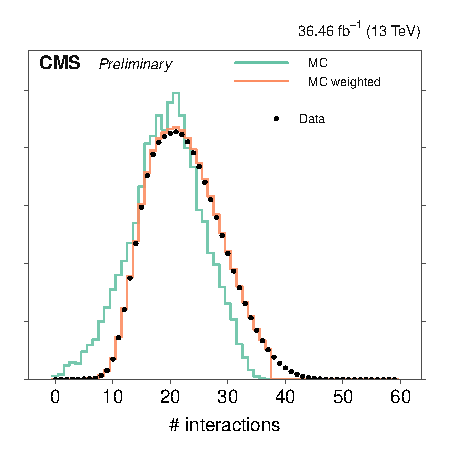
\includegraphics[scale=1.00]{figures/pileup_reweighting/f044_corr_nTrueInt_data_mc_norm}
\caption{The distribution of the average numbers of the inelastic
interactions per colliding bunch pair per lumi section in the data,
corresponding distribution in the simulated events, and that of the
reweighted simulated events.} \label{f044_corr_nTrueInt_data_mc_norm}
\end{figure}


\subsection{Cross sections for SM samples}
\label{sec:SMxs}
Several MC samples of individual SM processes are binned according to a generator level quantity, 
such as the partonic \HT or bosonic \PT.
This analysis chooses to use samples binned in partonic \HT 
for the set of MC samples (W+jets, DY+jets, QCD, $\gamma$+jets, $Z\rightarrow \nu\nu$+jets).
These binned samples are provided with LO cross sections. 
The \kfactors required to go from LO to NNLO cross section are typically determined using corresponding
inclusive samples applied to each \HT binned sample.
Further studies can provide additional corrections to the cross sections, 
which can prove important to the closure test procedures described in
Section \ref{sec:closure-tests}. As can be seen in Section~\ref{sec:sideband_corrections}, residual cross section
corrections are measured using data in sidebands designed to enrich specific processes.

In the $8\tev$ LHC results the shape of the top quark $p_{T}$ spectrum
was found to differ between simulation and data. A reweighting is
therefore applied to MC events that contain a generated top. The value of
this correction is provided from the $8\tev$ results, as described in
\cite{twiki-TopPtReweighting}.

The inclusive distributions of the MC samples
with respect to the binning variable
$H_{T}^{parton}$ are shown in Fig.~\ref{fig:Lhe_Ht}, with
the bin by bin derivative drawn below.

As can be seen in the distributions, the stitched samples
exhibit a good level of smoothness,
further demonstrated by the derivative which shows a flat trend for each 
cross section.

A more in depth and data-driven investigation of the cross sections is shown in Sec.~\ref{sec:sideband_corrections}. 
Of which, an important point to note is that the corrections to the cross sections, 
derived with the data sidebands are only relevant for Data/MC comparison plots and the suite of closure tests defined in Section \ref{sec:closure-tests}.

\begin{figure}[!h]
  \begin{center}
    \subfigure[$Z\rightarrow \nu\nu$ +jets] {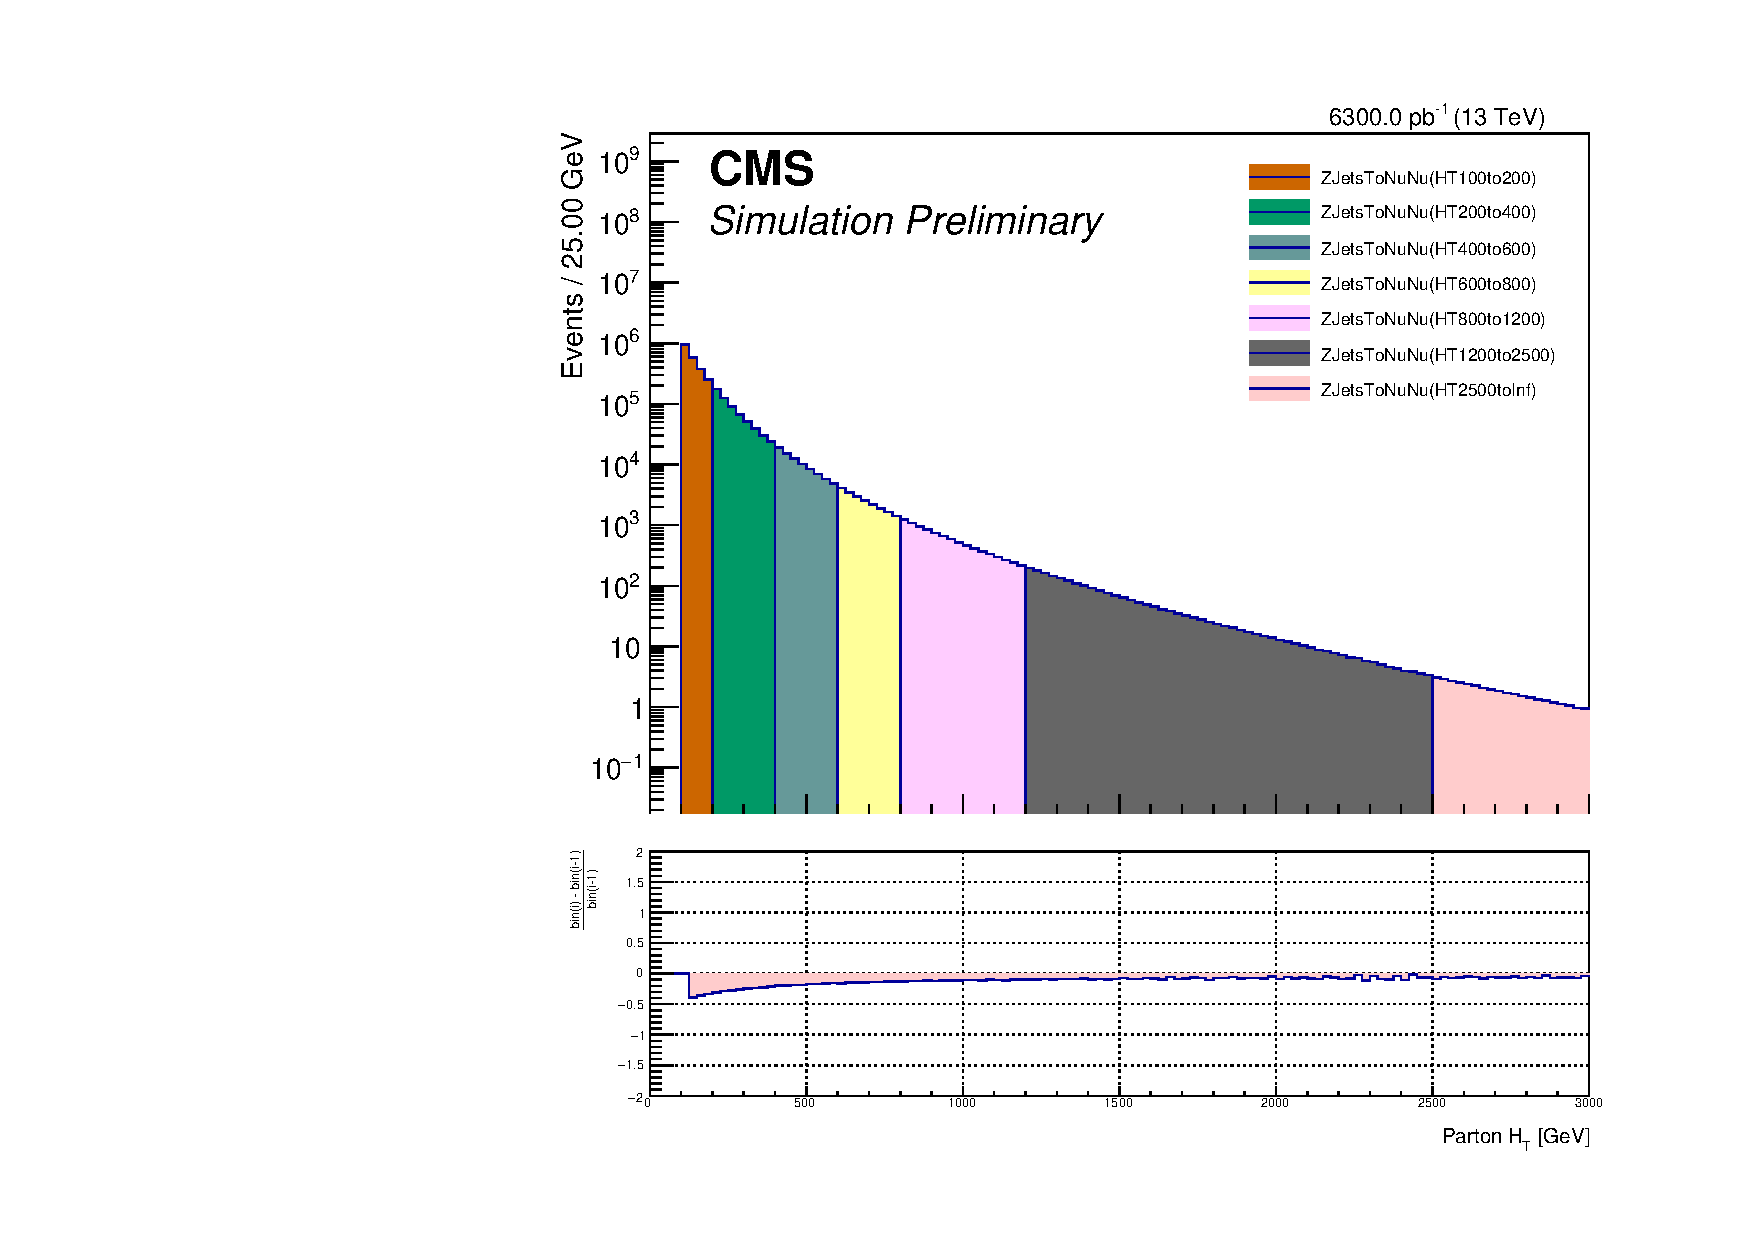
\includegraphics[width=0.40\textwidth]{figures/binnedMCsamples/2016/6p3/Zinv.pdf}} ~~
    \subfigure[$W\rightarrow l \nu$ + jets]{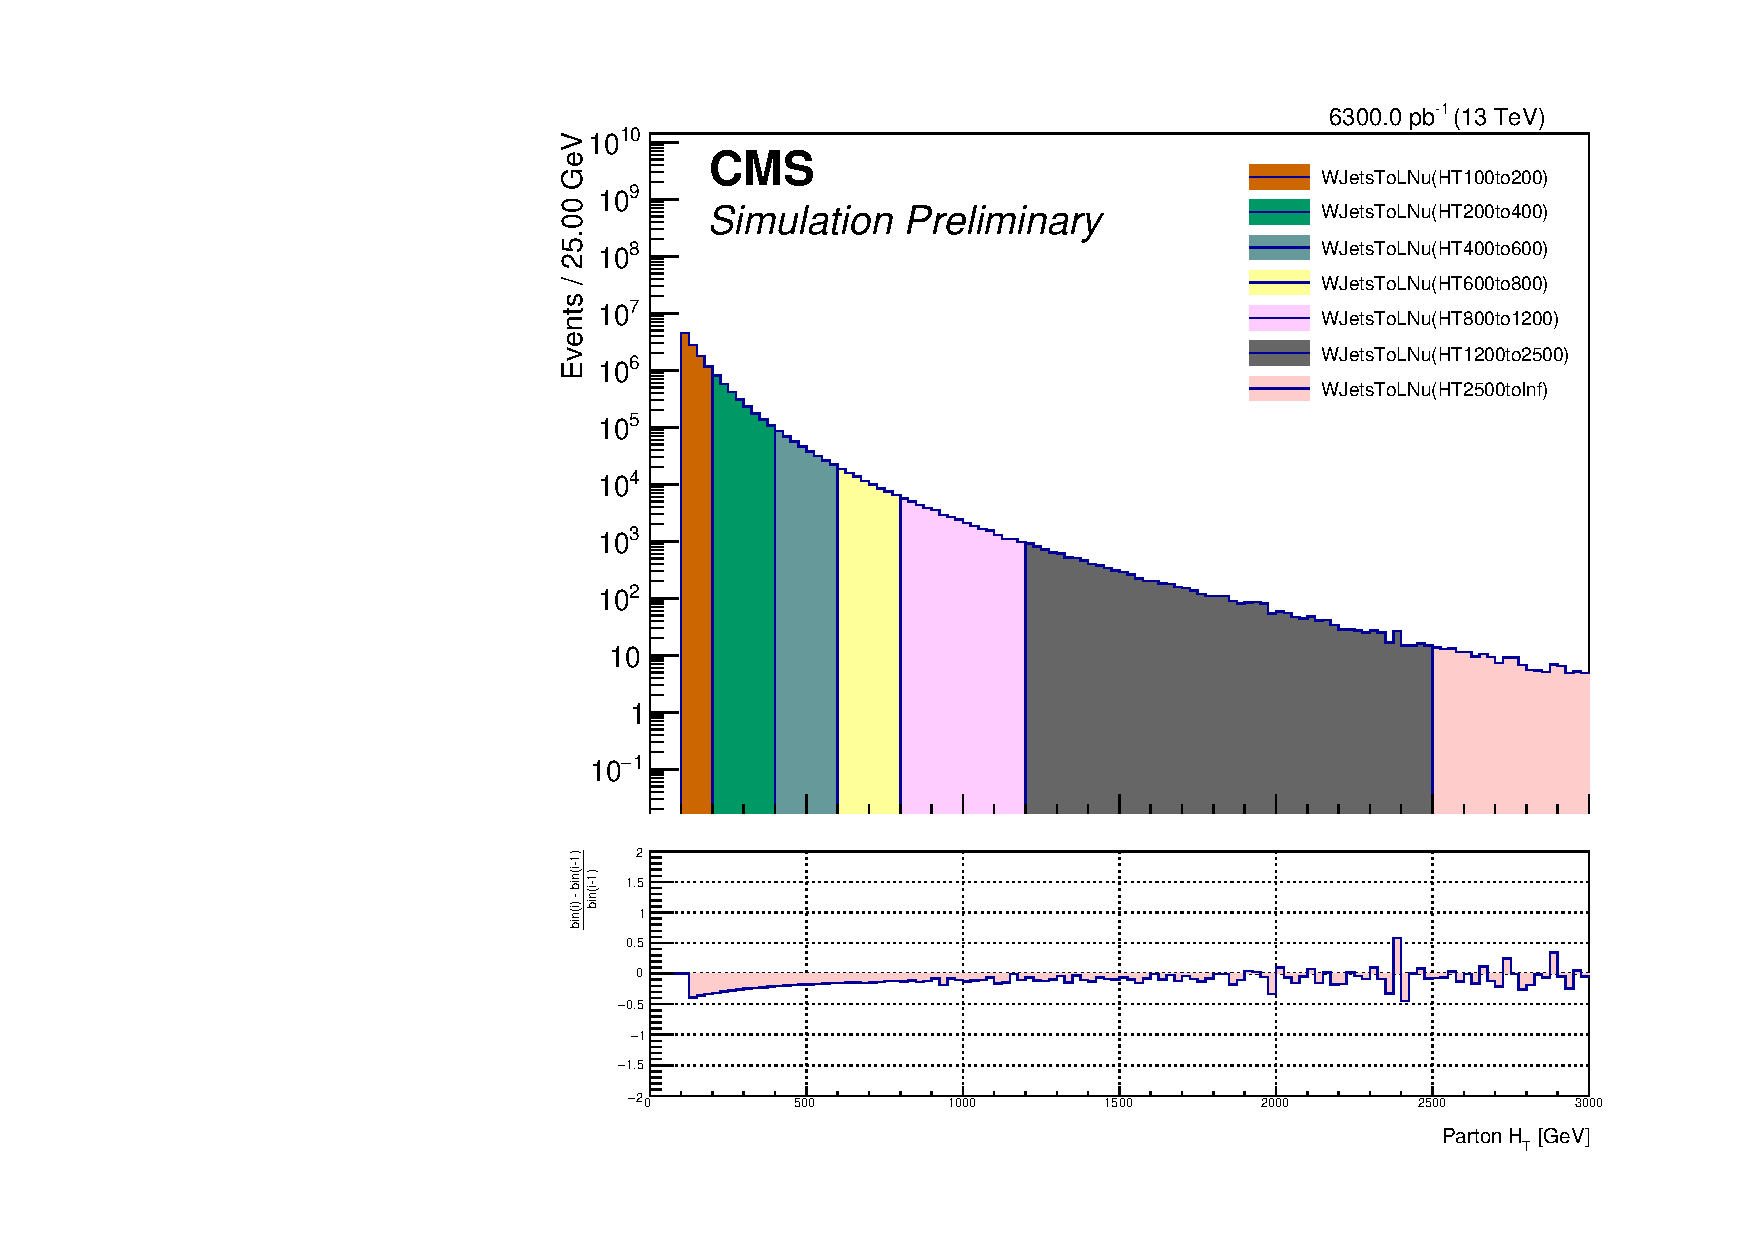
\includegraphics[width=0.40\textwidth]{figures/binnedMCsamples/2016/6p3/WJetsToLNu_HT.pdf}} \\
    \subfigure[$DY\rightarrow ll$ + jets]{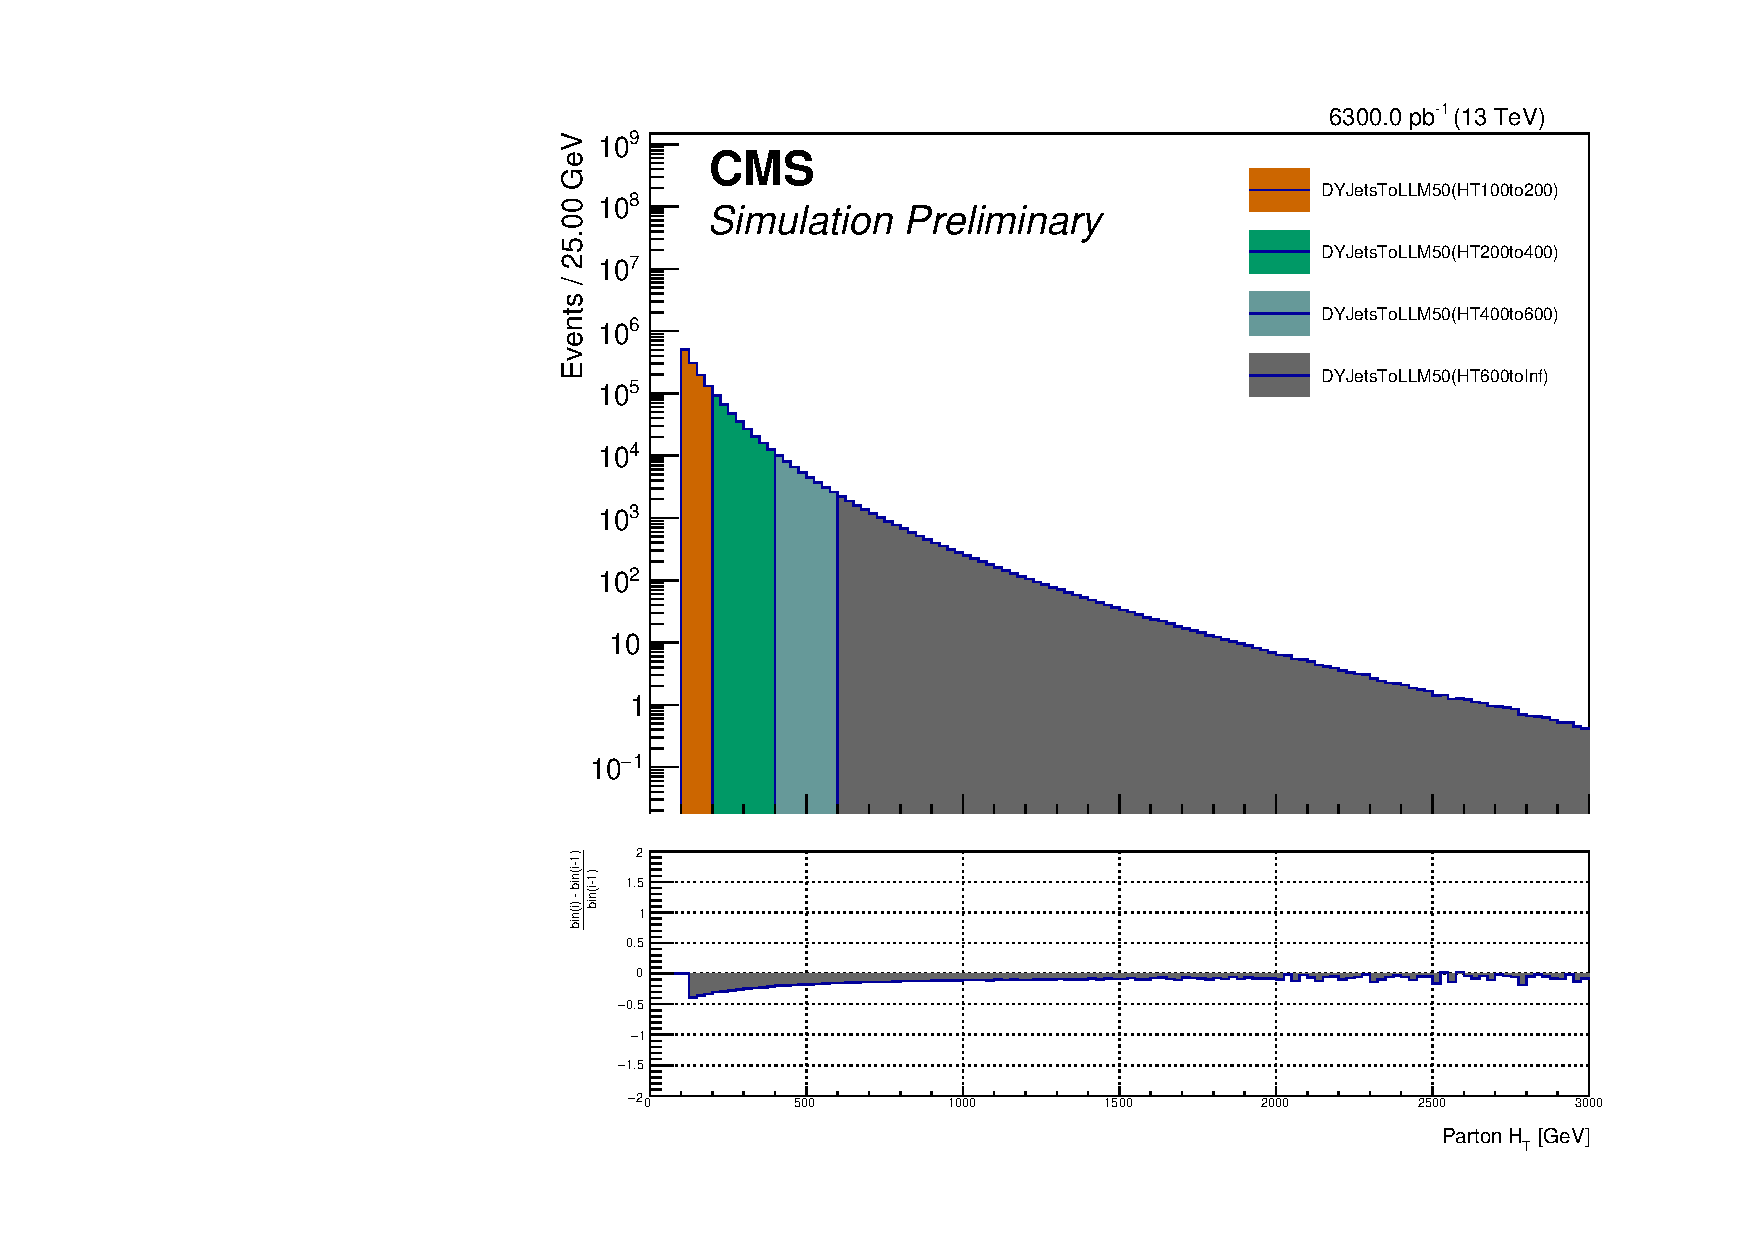
\includegraphics[width=0.40\textwidth]{figures/binnedMCsamples/2016/6p3/DYJetsToLL_M50_HT.pdf}} ~~
    \subfigure[QCD]{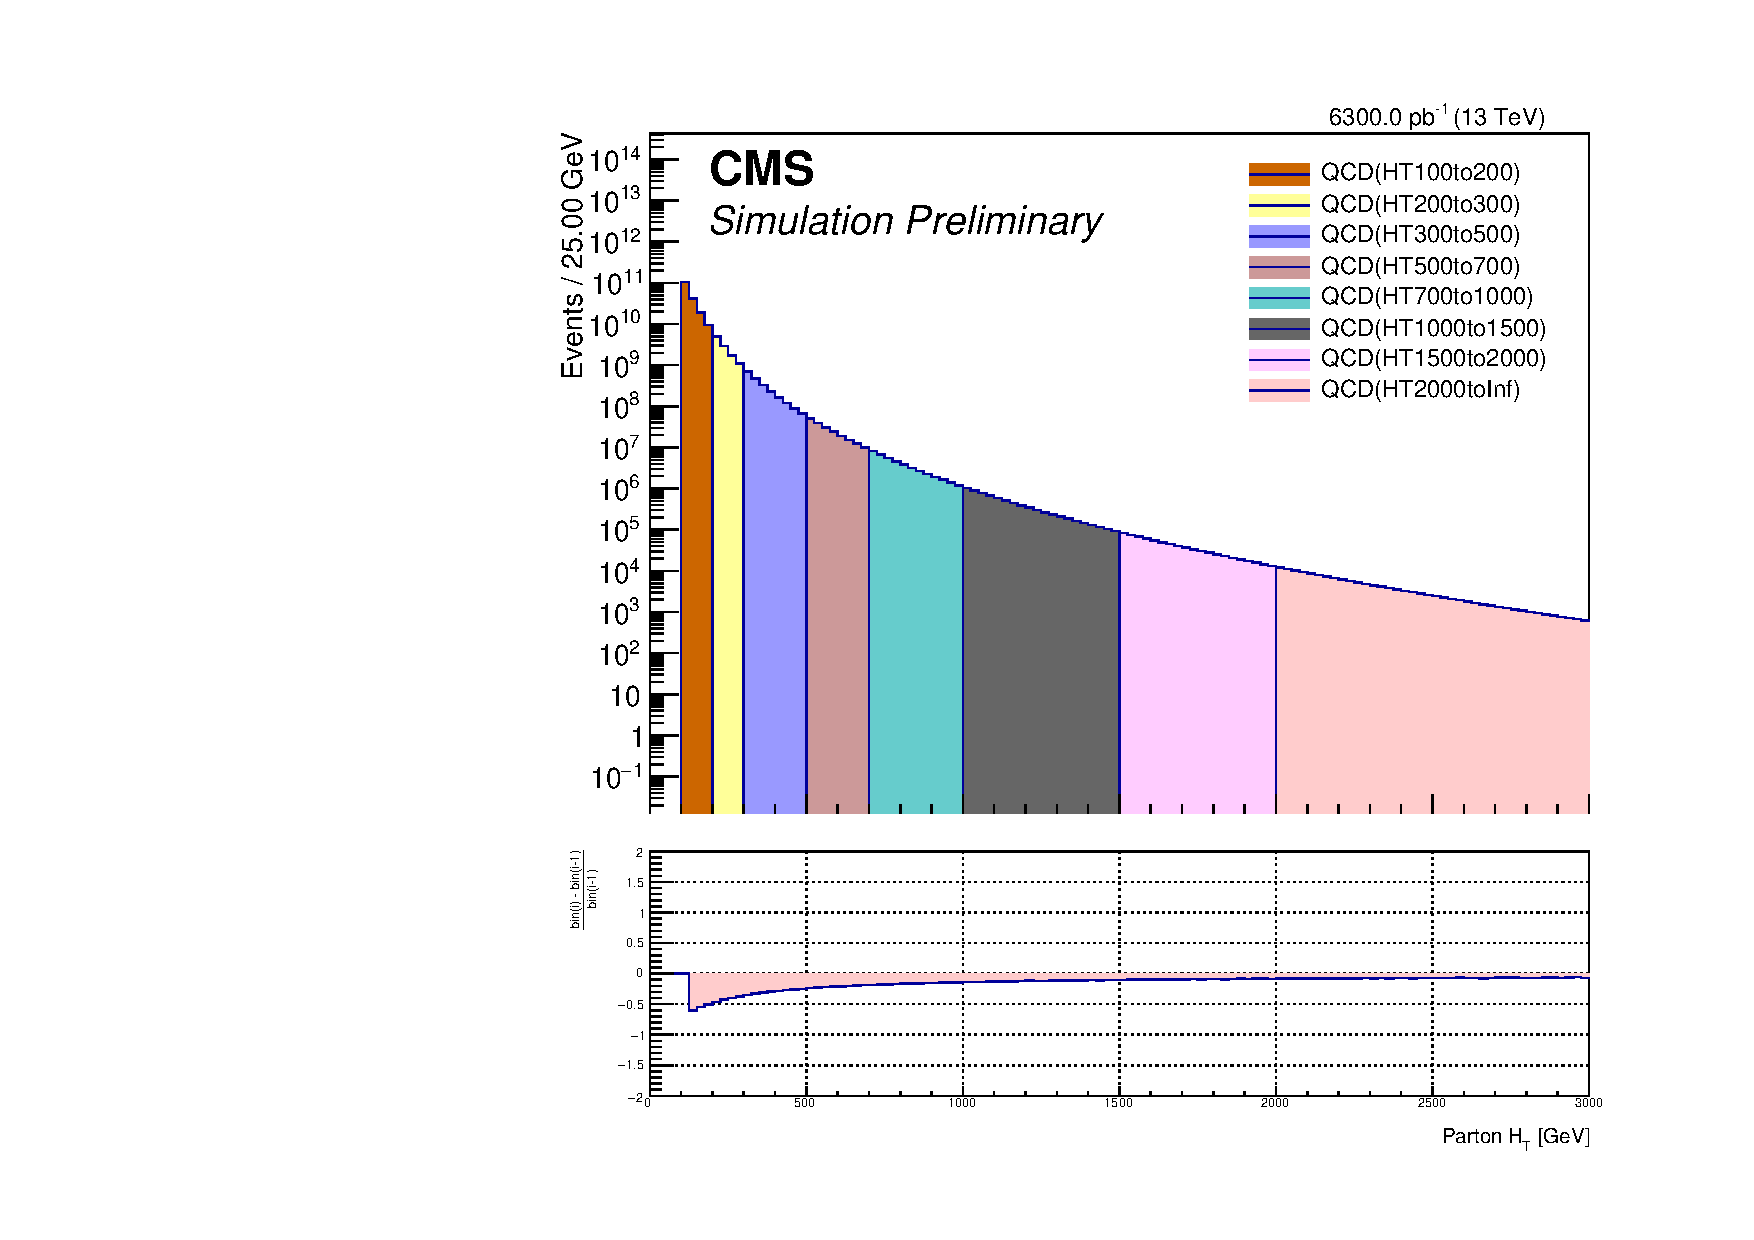
\includegraphics[width=0.40\textwidth]{figures/binnedMCsamples/2016/6p3/QCD_HT.pdf}} \\
    \subfigure[$\gamma$+jets]{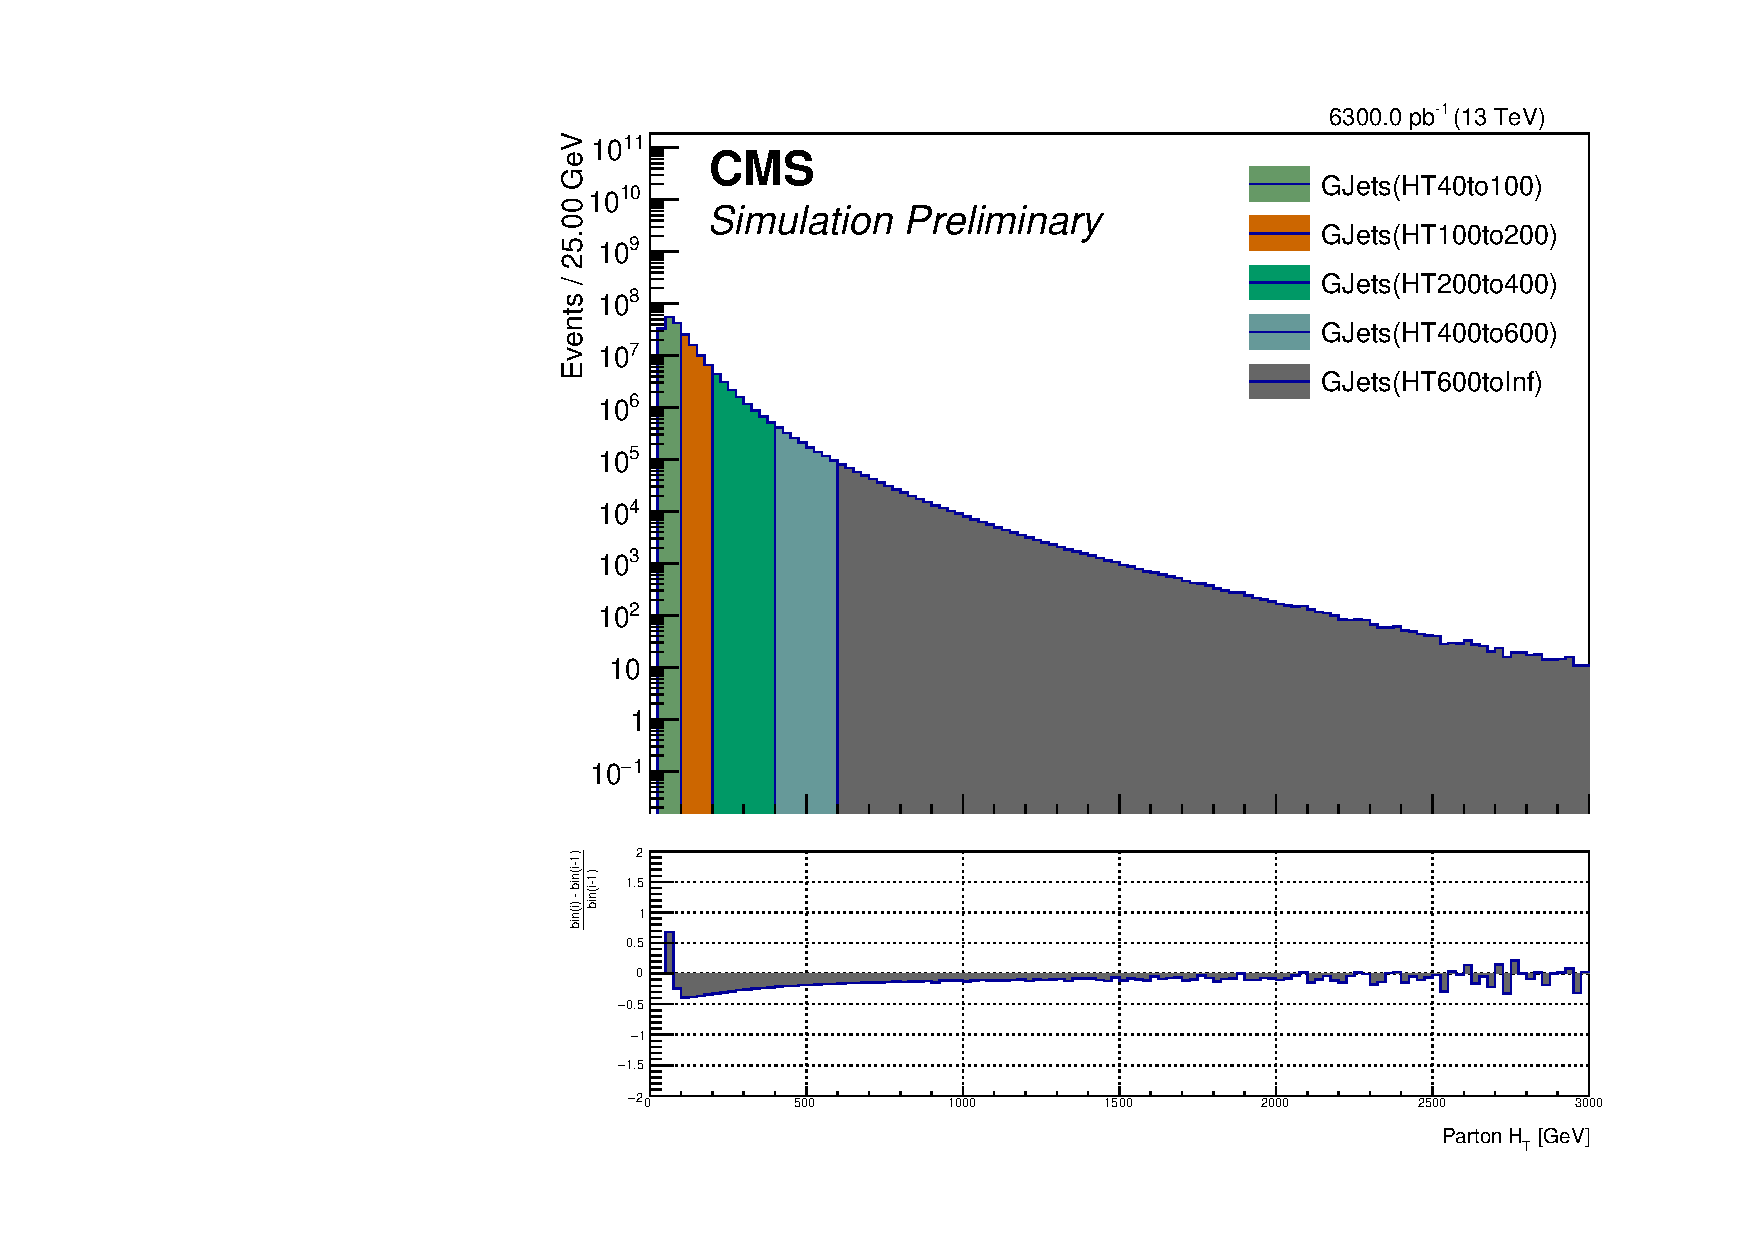
\includegraphics[width=0.40\textwidth]{figures/binnedMCsamples/2016/6p3/GJets_HT.pdf}} ~~
    \caption{Generator-level $H_{T}^{parton}$ distributions for SM process, $Z\rightarrow \nu\nu$ + jets, W+jets, DY+jets, QCD and $\gamma$+jets}
    \label{fig:Lhe_Ht}
  \end{center}
\end{figure}

%%____________________________________________________________________________||

%% %%____________________________________________________________________________||
\section{Trigger strategy}
\label{sec:triggers}

\subsection{Signal regions\label{sec:hadronic_signal_region}}

In Run~2 the RA1 analysis retains the low-thresholds of Run~1 with developments 
to the trigger selection, maintaining sensitivity to signatures of new physics with hadronic 
energies as low as $\scalht = 200$ GeV. This in part is achieved by a migration to PF-based 
jet reconstruction within the HLT which, in conjunction with a reduction of clustering radius 
parameter $\Delta R = 0.4$, provides improvements in jet energy resolution in high-pileup 
conditions and mitigates the effects of pileup contamination within the jet cone.

The RA1 analysis utilises a range of triggers for the selection of events in the hadronic signal region
to provide coverage over a wide range of event topologies. A guiding principle of the analysis is to be as
inclusive as possible by probing low thresholds, necessitating operation in or near the trigger turn-on.
Events in the hadronic monojet signal region are selected with the use of the
lowest unprescaled \mht-\met cross-trigger, 
\verb!HLT_PFMETNoMuXX_PFMHTNoMuXX_IDTight!, which is cross-cleaned of muons in the computation 
of event variables in the HLT.

The hadronic multijet signal region is selected by a suite of $\scalht$-$\alphat$ cross-triggers 
with a requirement on the average \pt of the leading two jets, $\pt^{\rm \left<j1,j2\right>}$, labelled: 
\verb!HLT_PFHTXXX_PFDijetYYY_AlphaT0pZZ!. The use of a dijet average threshold provides an improved 
suppression of QCD multijet events within the trigger,
enabling looser \alphat thresholds to be utilised whilst maintaining acceptance to events exhibiting asymmetric jet 
topologies such as monojet-like signatures of compressed spectrum and DM models. It was found that a dijet average
threshold of 90 \GeV ensured the optimum performance when balancing efficiency and rate, with both the $\scalht$ and $\alphat$
thresholds across all jet topologies. The dijet average requirement does however lead to a loss in efficiency for 
asymmetric jet events where the sub-leading jet is soft.

This loss in efficiency is mitigated by taking the 
disjunction of the \alt and monojet triggers which provides a recovery 
of efficiency in the turn-on and close to the plateau for the low-\scalht asymmetric categories. 
Above $\scalht > 800$ \GeV an additional pure \scalht trigger, \verb!HLT_PFHT800!, 
is also utilised which has no explicit dependence on $\alphat$ or dijet average threshold. 

These triggers form the primary signal selection menu for the analysis. In
addition, a set of secondary triggers with higher thresholds are in operation 
to provide redundancy for higher luminosity scenarios. In the $1\times10^{34}\cm^{-2}{\rm s}^{-1}$
luminosity scenario, the \verb!HT200! \alphat seed path is prescaled and is replaced by
its backup path. Similarly, the backup paths of the \verb!HT250! and \verb!HT300!
triggers are utilised at $1.2\times10^{34}\cm^{-2}{\rm s}^{-1}$ and
$1.4\times10^{34}\cm^{-2}{\rm s}^{-1}$, respectively. All other \alphat
paths sufficiently suppress trigger rates such that the use of secondary triggers 
are not required in these cases.

The Level-1 seeds for the $\scalht$-$\alphat$ HLT paths are given by the
disjunction of all available hadronic scalar energy and missing energy sum seeds for 
the given run scenario. A loose calorimeter trigger prefilter is utilised to reduce the pass-through 
rate prior to track-based reconstruction, ensuring the PF-based filters meet timing requirements. The calorimeter prefilter 
utilises loose \scalht and dijet average \pt requirements in addition to a new variable \alphat', 
defined as \alphat in the limit $\Delta\scalht \rightarrow 0$, which better correlates \alphat 
between calorimeter and PF-based reconstruction. 
%The monojet and \verb!HLT_HT800! triggers use the
%\verb!ETM50! and \verb!HTT175! seeds respectively with loose \mht and \scalht prefilters to suppress pass-through rate.

The thresholds of the signal triggers are shown in Table~\ref{tab:2015_Hadronic_Signal_Triggers}. The choice of threshold for 
the \scalht-\alphat triggers were tuned to maintain acceptance for a range of signal topologies whilst effectively suppressing QCD 
multijet events to maintain acceptable trigger rates. 


\begin{table}[h!]
\topcaption{Trigger thresholds of the Level-1, calorimeter prefilter and final PF-trigger decision for
 the primary HLT paths for the hadronic signal region in the  $\lumi=7\times10^{33}\cm^{-2}{\rm s}^{-1}$ scenario.
 The L1 seeds correspond to the lowest threshold unprescaled ones available, which vary as a function of instantaneous luminosity. }
\footnotesize
\centering
\begin{tabular}{c|cccc} 
\hline
\hline
HLT path     & L1 seed & HLT calo-prefilter & HLT PF-filter                                                \\
    &        & ($\scalht$, $\alphat$', $\pt^{\rm \left<j1,j2\right>}$, \met) & ($\scalht$, $\alphat$, $\pt^{\rm \left<j1,j2\right>}$, \met) \\ %& (Hz) \\[0.7 ex] 
\hline
{\scriptsize \verb!HLT_PFHT200_PFDijetAve90_AlphaT0p57!} & {\scriptsize\verb!HTT240 OR ETM70!} & 150, 0.540, 70, - & 200, 0.570, 90, - \\ %& \\ % 11.0 $\pm$ 3.0 \\
{\scriptsize \verb!HLT_PFHT250_PFDijetAve90_AlphaT0p55!} & {\scriptsize\verb!HTT240 OR ETM70!} & 200, 0.535, 70, - & 250, 0.550, 90, - \\ %& \\ % 8.5  $\pm$ 3.0 \\
{\scriptsize \verb!HLT_PFHT300_PFDijetAve90_AlphaT0p53!} & {\scriptsize\verb!HTT240 OR ETM70!} & 250, 0.525, 70, - & 300, 0.530, 90, - \\ %& \\ % 9.5  $\pm$ 3.0 \\
{\scriptsize \verb!HLT_PFHT350_PFDijetAve90_AlphaT0p52!} & {\scriptsize\verb!HTT240 OR ETM70!} & 300, 0.520, 70, - & 350, 0.520, 90, - \\ %& \\ % 10.0 $\pm$ 3.0 \\
{\scriptsize \verb!HLT_PFHT400_PFDijetAve90_AlphaT0p51!} & {\scriptsize\verb!HTT240 OR ETM70!} & 370, 0.510, 70, - & 400, 0.510, 90, - \\ %& \\ % 13.5 $\pm$ 3.5 \\ \\ %\hline \\ %
{\scriptsize \verb!HLT_PFHT800!}                         & {\scriptsize\verb!HTT240!}          & 650, -, -, -      & 800, -, -, -, -   \\ %& \\ % 13.5 $\pm$ 3.5 \\ \\ %\hline \\ %
{\scriptsize \verb!HLT_PFMETNoMu90_PFMHTNoMu90_IDTight!} & {\scriptsize\verb!ETM70!}           &  -, -, -, -, 65   & -, -, -, -, 90    \\
%% L1sL1ETM70ORETM60ORETM50
%% hltMET, MHT 65
\hline
\hline
\end{tabular}
\label{tab:2015_Hadronic_Signal_Triggers}
\end{table}


An important goal of the analysis is to have good acceptance
to compressed SUSY and general DM models. It is therefore critical
that we operate in the trigger turn on regions for the lower
thresholds. We have already successfully exercised this approach with 
the Run 1 analysis and will repeat this mode or operating during Run 2.
As in Run~1, multiple efficiency measurements are
employed, which are performed with data and propagated through to the
analysis with cross checks in simulation. 
%% A summary of estimates of a selection of signal models in simulation is presented in Appendix~\ref{app:signalModelTriggerEfficiencies}.

%% However, it is noted that for the majority of models accessible by the
%% "Early Analysis", such as gluino-induced production and decay, the
%% most sensitive bins are typically at higher values of MHT, for which
%% the triggers perform close to full efficiency. Lower MHT bins are
%% subject to trigger efficiency corrections based on measurements in
%% data, as discussed above. 


The efficiency of the signal triggers are measured in data using electron and muon samples 
selected by the unprescaled \verb!HLT_Ele23_eta2p1_WPLoose_Gsf! and \verb!HLT_IsoMu20! 
reference triggers with a signal region selection. Biases in these measurements can be introduced 
due to the contamination in the computation of event variables and different treatments 
between trigger and offline reconstructions, the degree of which varies with
\scalht and \njet. In the case of efficiency measurements using the electron
reference trigger, no cross-cleaning of electrons from jets is performed
offline, with the electron being included in the computation of event-level jet
energy sums, such as \scalht, \MHT and \alt.

%The monojet trigger performs a cross-cleaning of muons online, enabling its efficiency to measured
%in an unbiased manner using a muon sample. Electrons however cannot be disentangled and to remain 
%consistent with the trigger must be measured with offline cross-cleaning disabled. A comparison of 
%the estimate of the monojet trigger efficiency using muon and electron samples is shown in Fig.~\ref{fig:monojet_turnons}.
%With consistent cross-cleaning of the muon online and offline the monojet trigger is measured to be fully efficient
%by \scalht = 300 \GeV consistent with measurements in simulation. Measured in an electron sample with no cross-cleaning however
%the trigger is measured to have an inefficiency which increases with \scalht. The bias leptons introduce when no cross-cleaning
%is applied is dominant for low-\scalht resulting in the disagreement between samples, this however becomes less important at high
%\scalht and \njet. With a proper treatment of cross-cleaning of muons online a muon sample is thought to provide a faster
%turn-on.

%\begin{figure}[h!]
%  \begin{center}
%    \subfigure[Muon sample]{\includegraphics[width=0.5\textwidth]{figures/Trigger/HLT_IsoMu20/HLT_PFMETNoMu90_JetIdCleaned_PFMHTNoMu90_IDTight_MoM_Mono_MHT0_ht.pdf}} ~~     
%    \subfigure[Electron sample]{\includegraphics[width=0.5\textwidth]{figures/Trigger/HLT_Ele23_eta2p1_WPLoose_Gsf/HLT_PFMETNoMu90_JetIdCleaned_PFMHTNoMu90_IDTight_MoM_Mono_MHT0_ht.pdf}} \\
%    \caption{Trigger efficiency of the monojet trigger measured in muon and electron samples.
%          }
%    \label{fig:monojet_turnons}
%  \end{center} 
%\end{figure}


%The multijet triggers do not have the muon cross-cleaning applied online so their efficiency measurement in data 
%is primarily performed with the use of an electron sample. To remain consistent with the 
%reconstruction of electrons in the trigger, no cross-cleaning of electrons from jets 
%are performed offline, with the electron being included in the computation of event-level jet energy sums, such as 
%\scalht, \MHT and \alt. The turn-on for the individual \scalht-\alphat triggers are shown in Appendix~\ref{app:alphaTTriggerEfficiencies}

The trigger efficiency of the multijet triggers as a function of \mht after a full signal selection 
is shown in Figs.~\ref{fig:alphat_turnons_sym},\ref{fig:alphat_turnons_asym},\ref{fig:alphat_turnons_mono}, and is shown to be close to or at the plateau when taking 
the disjunction of triggers. These efficiencies are measured in bins of \scalht and \mht
per jet topology (monojet, symmetric and asymmetric). The measured
efficiencies and their uncertainties are applied as corrections to the MC
samples. The central value of the correction is taken from the efficiency
measured with the muon reference trigger. The difference in efficiencies between
those measured with the electron and muon triggers, together with the
statistical uncertainty of the muon measurement, is propagated as a systematic
uncertainty. The efficiencies have also been checked in bins of \njet and show
no significant dependence on \njet (see Appendix~\ref{app:alphaTTriggerEfficiencies}).
%for \scalht < 800 \GeV. The efficiency without a proper cross-cleaning
%is predicted to be exceed that measured with electron bias. A full efficiency is therefore assumed for 
%these triggers with a systematic to this estimate assigned equal to the
%inefficiency estimated by the respective reference trigger. 
%For \scalht $> 800$ \GeV, where the bias of electrons is a smaller effect, the trigger 
%efficiency is measured for the disjunction of the \scalht-\alphat and \verb!HLT_HT800! triggers, inclusively on jet multiplicity, and a correction applied which is shown in Fig.~\ref{fig:ht800_turnons}. 

The turn-ons for the individual \scalht-\alphat triggers are shown in
Appendix~\ref{app:alphaTTriggerEfficiencies}.

\begin{figure}[h!]
  \begin{center}
    \subfigure[$200 < \scalht < 250$]{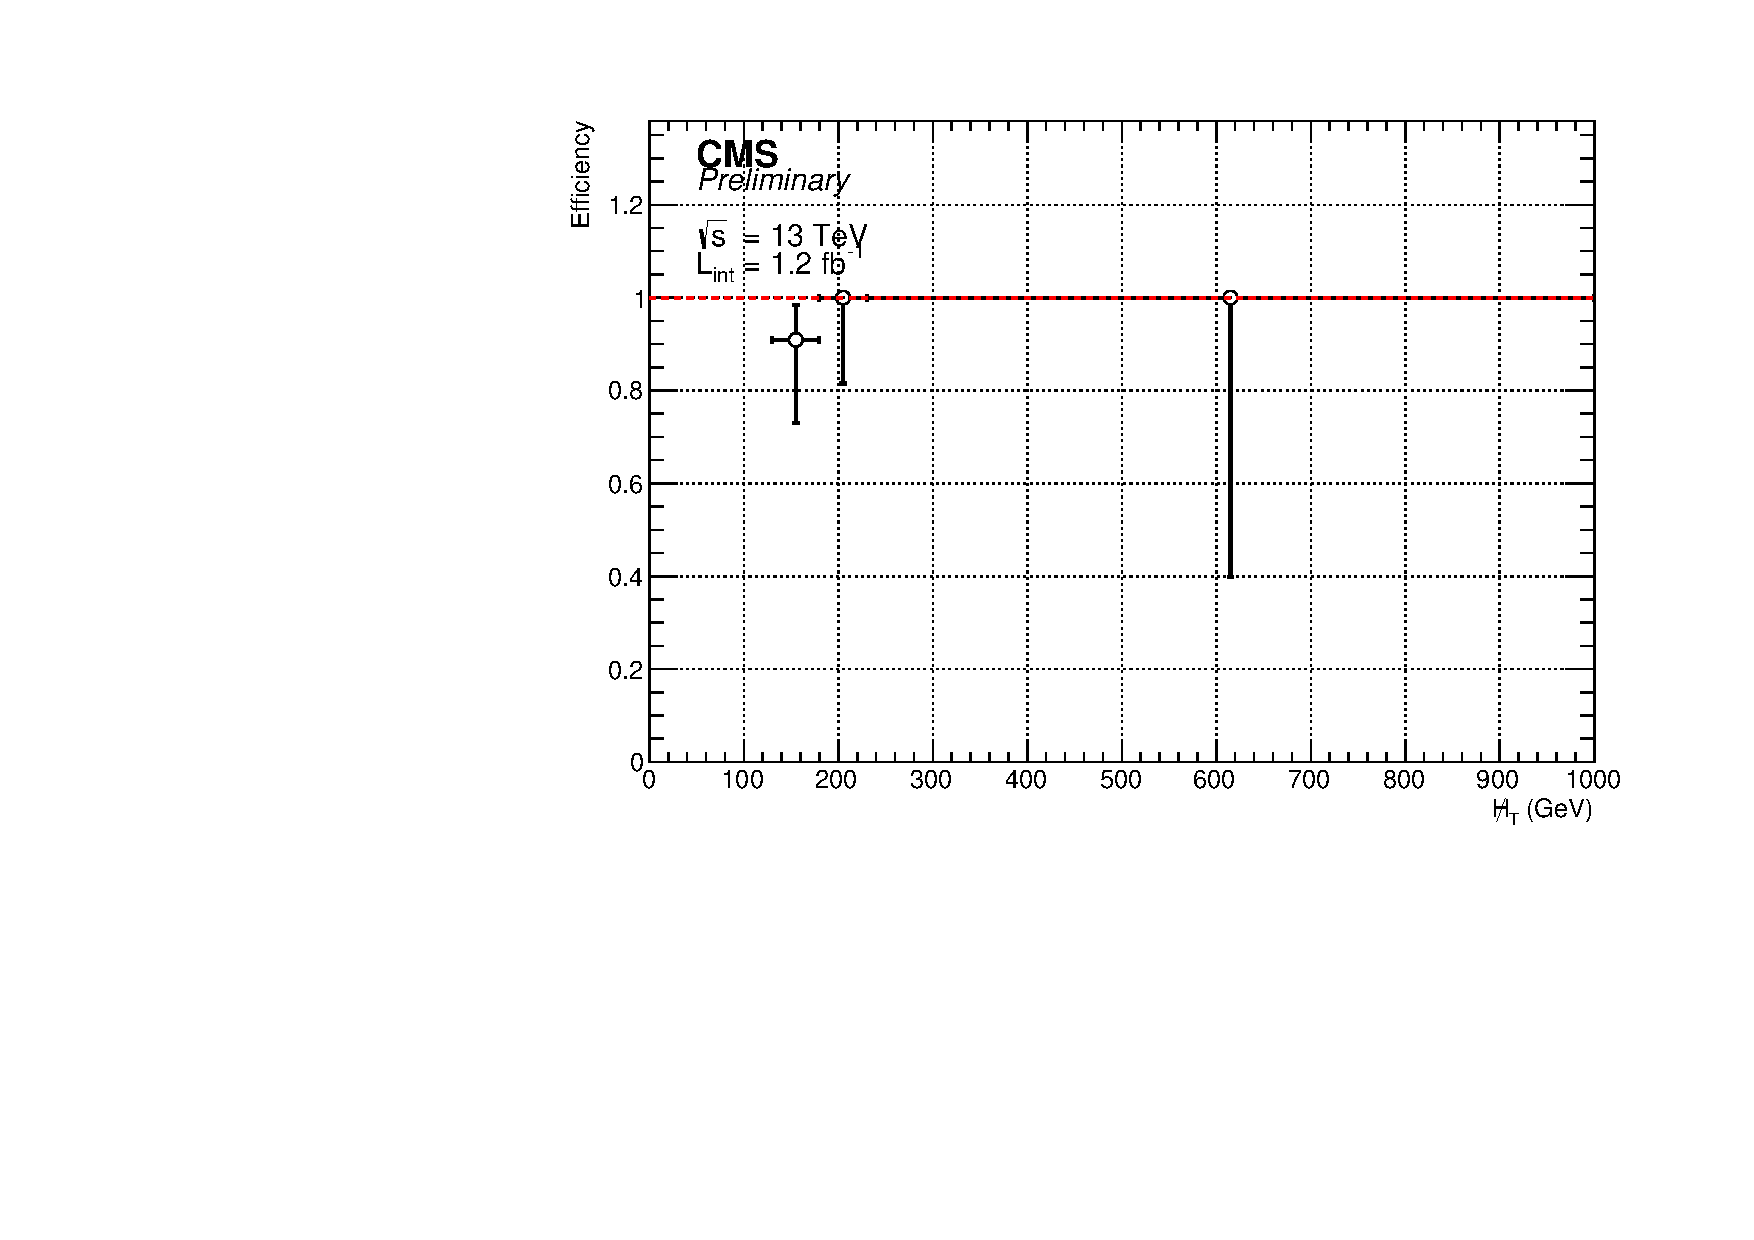
\includegraphics[width=0.4\textwidth]{figures/Trigger/HLT_IsoMu22/HLT_AlphaTMonoAll_MoM_200to250_mht}} ~~\
    \subfigure[$300 < \scalht < 350$]{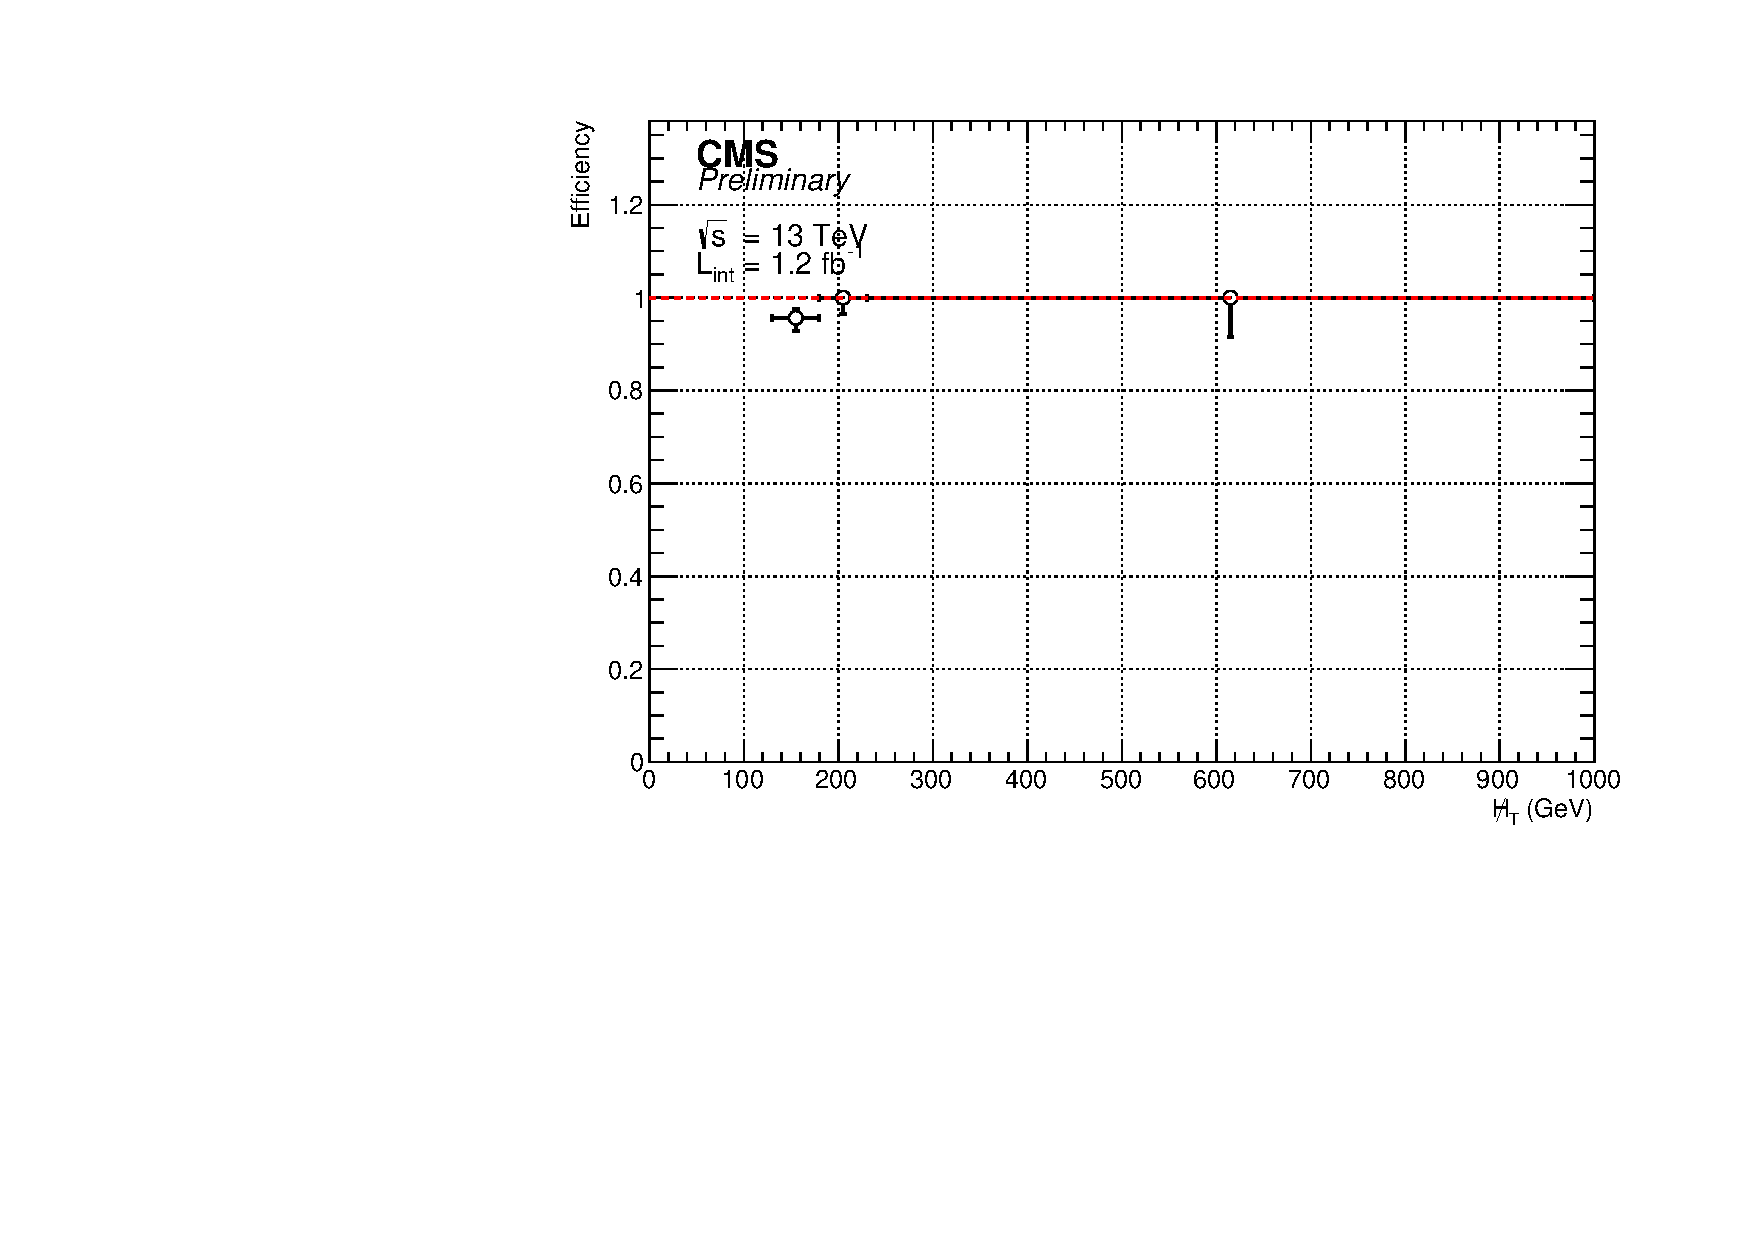
\includegraphics[width=0.4\textwidth]{figures/Trigger/HLT_IsoMu22/HLT_AlphaTMonoAll_MoM_300to350_mht}} \\
    \subfigure[$400 < \scalht < 600$]{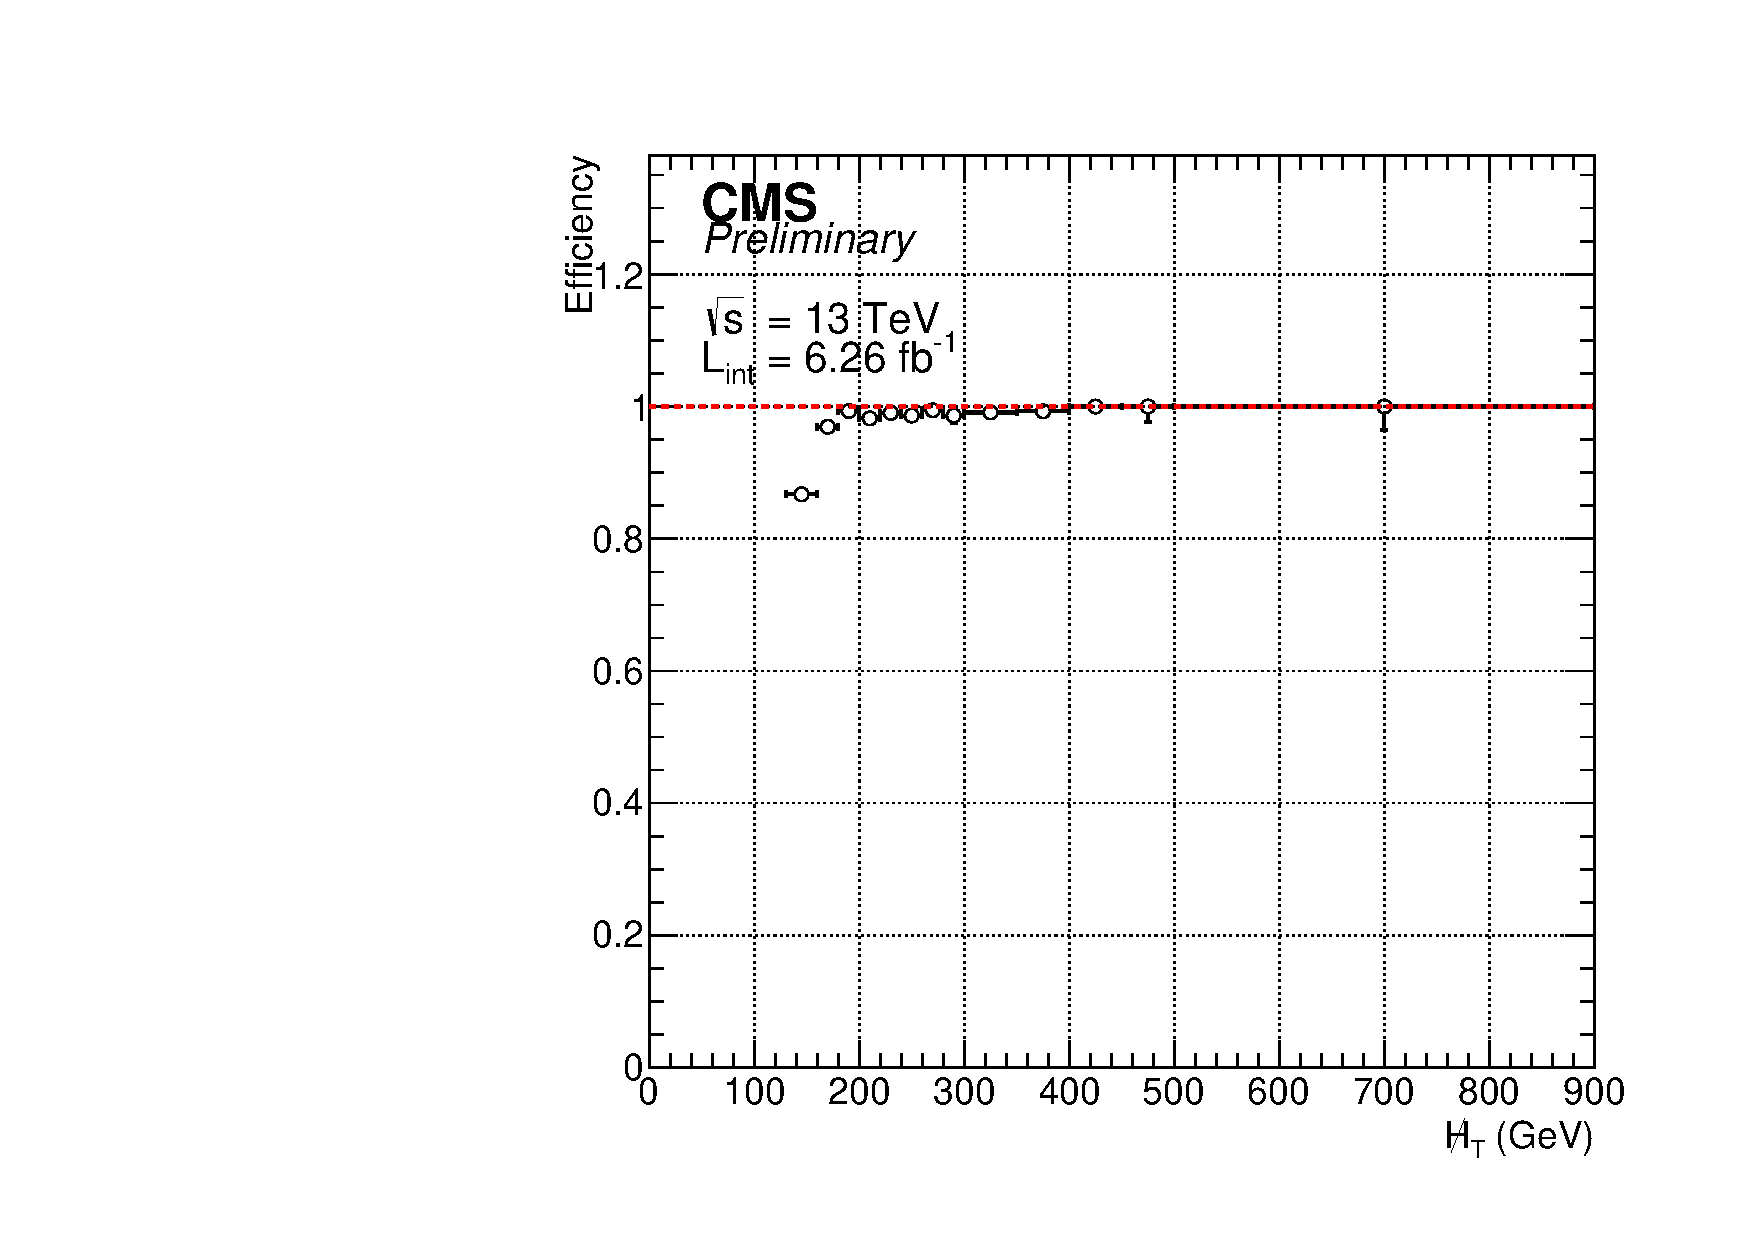
\includegraphics[width=0.4\textwidth]{figures/Trigger/HLT_IsoMu22/HLT_AlphaTMonoAll_MoM_400to600_mht}} ~~\
    \subfigure[$600 < \scalht < 800$]{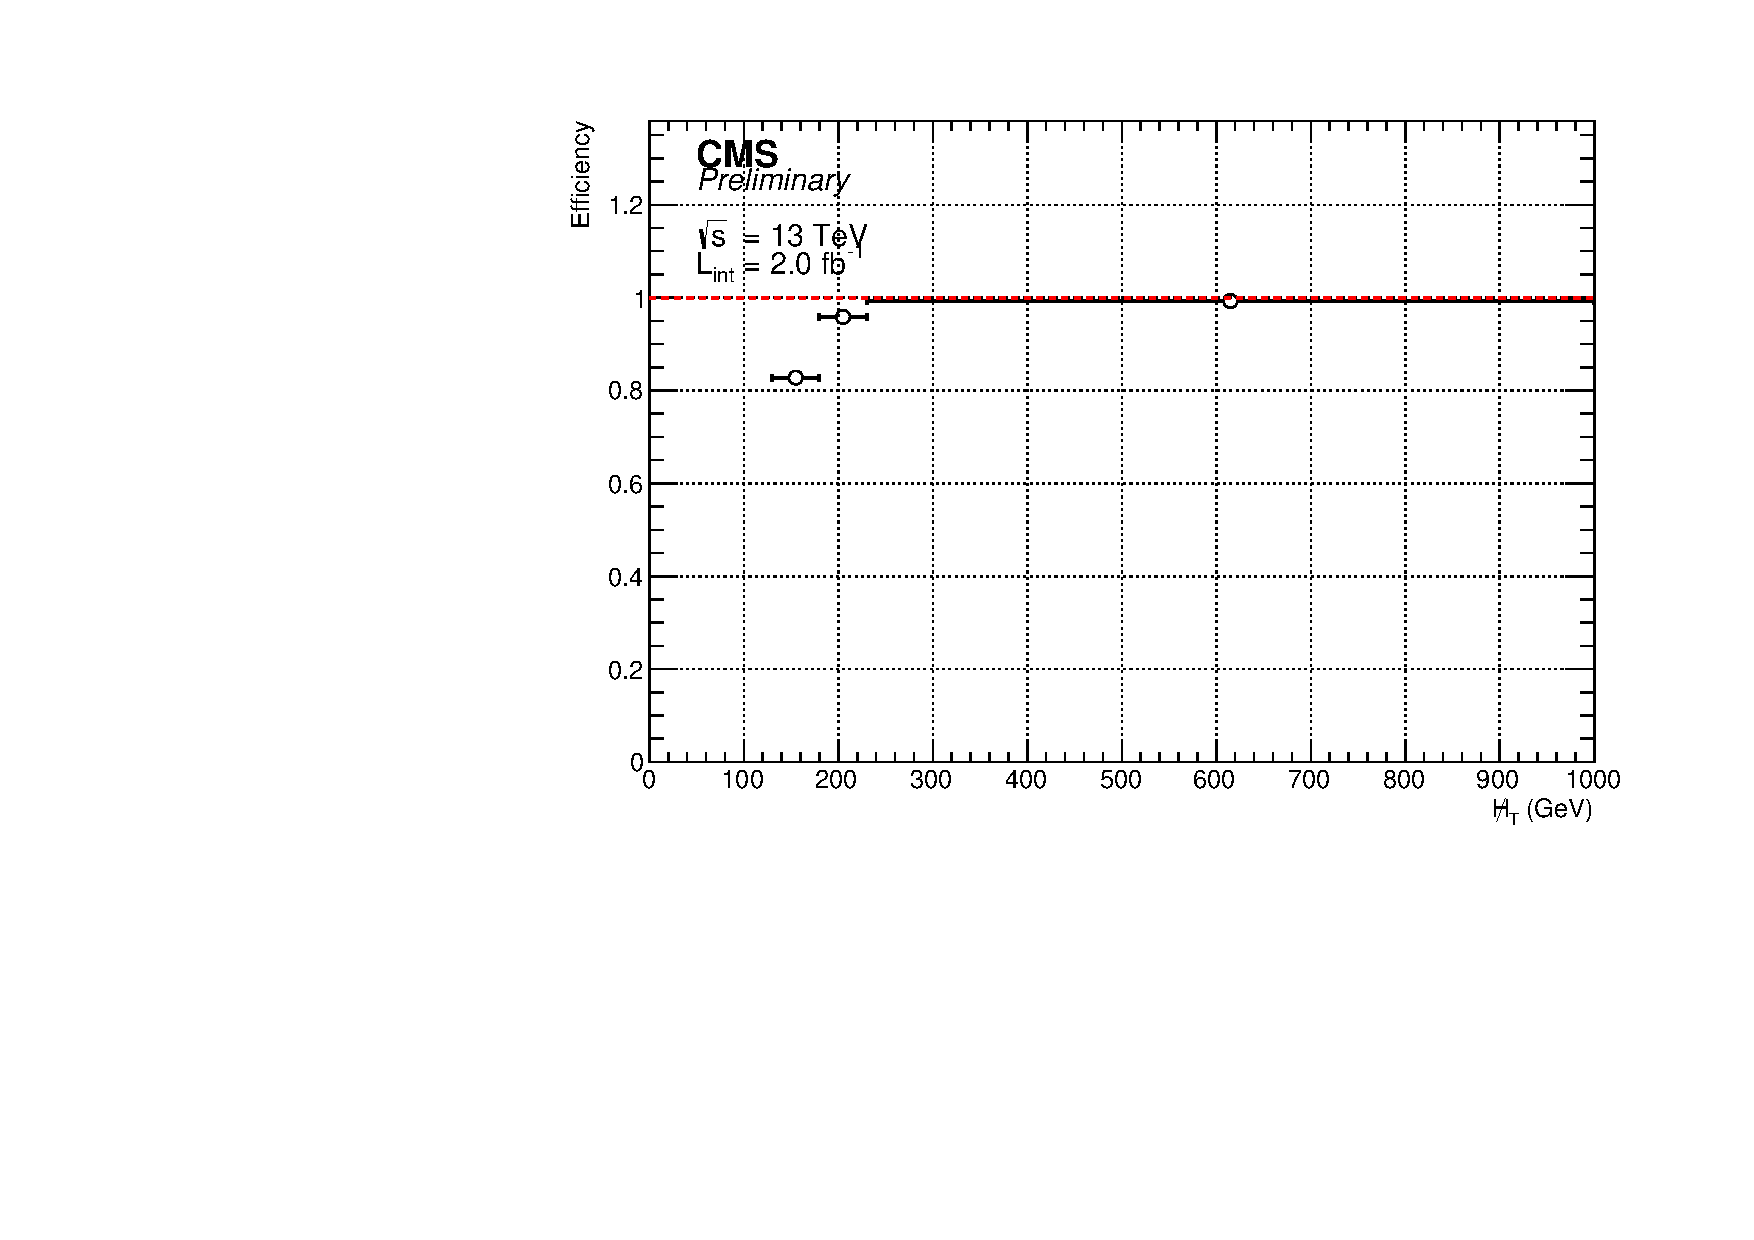
\includegraphics[width=0.4\textwidth]{figures/Trigger/HLT_IsoMu22/HLT_AlphaTMonoAll_MoM_600to800_mht}} \\
    \subfigure[$800 < \scalht < 850$]{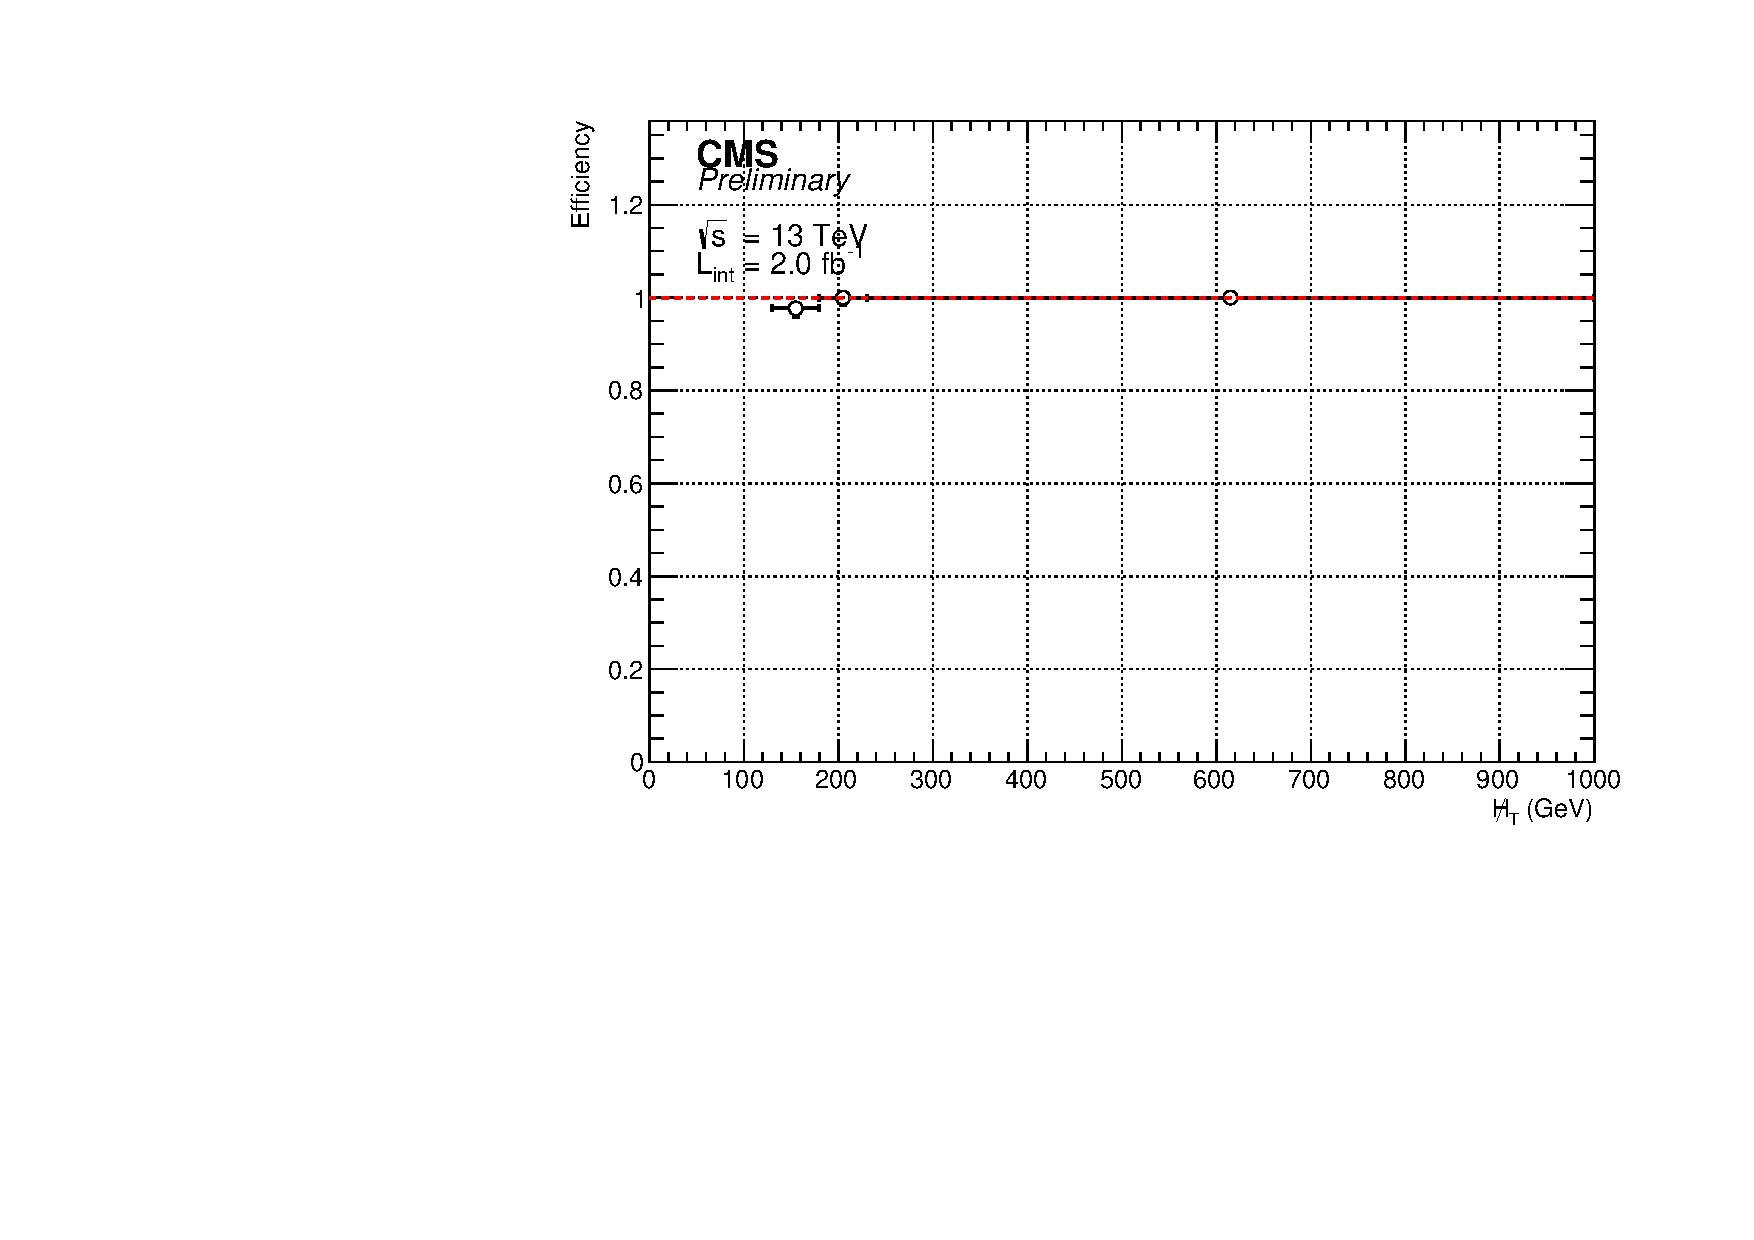
\includegraphics[width=0.4\textwidth]{figures/Trigger/HLT_IsoMu22/HLT_AlphaTHT800MonoAll_MoM_800to850_mht}} ~~\
    \subfigure[$\scalht > 900$]{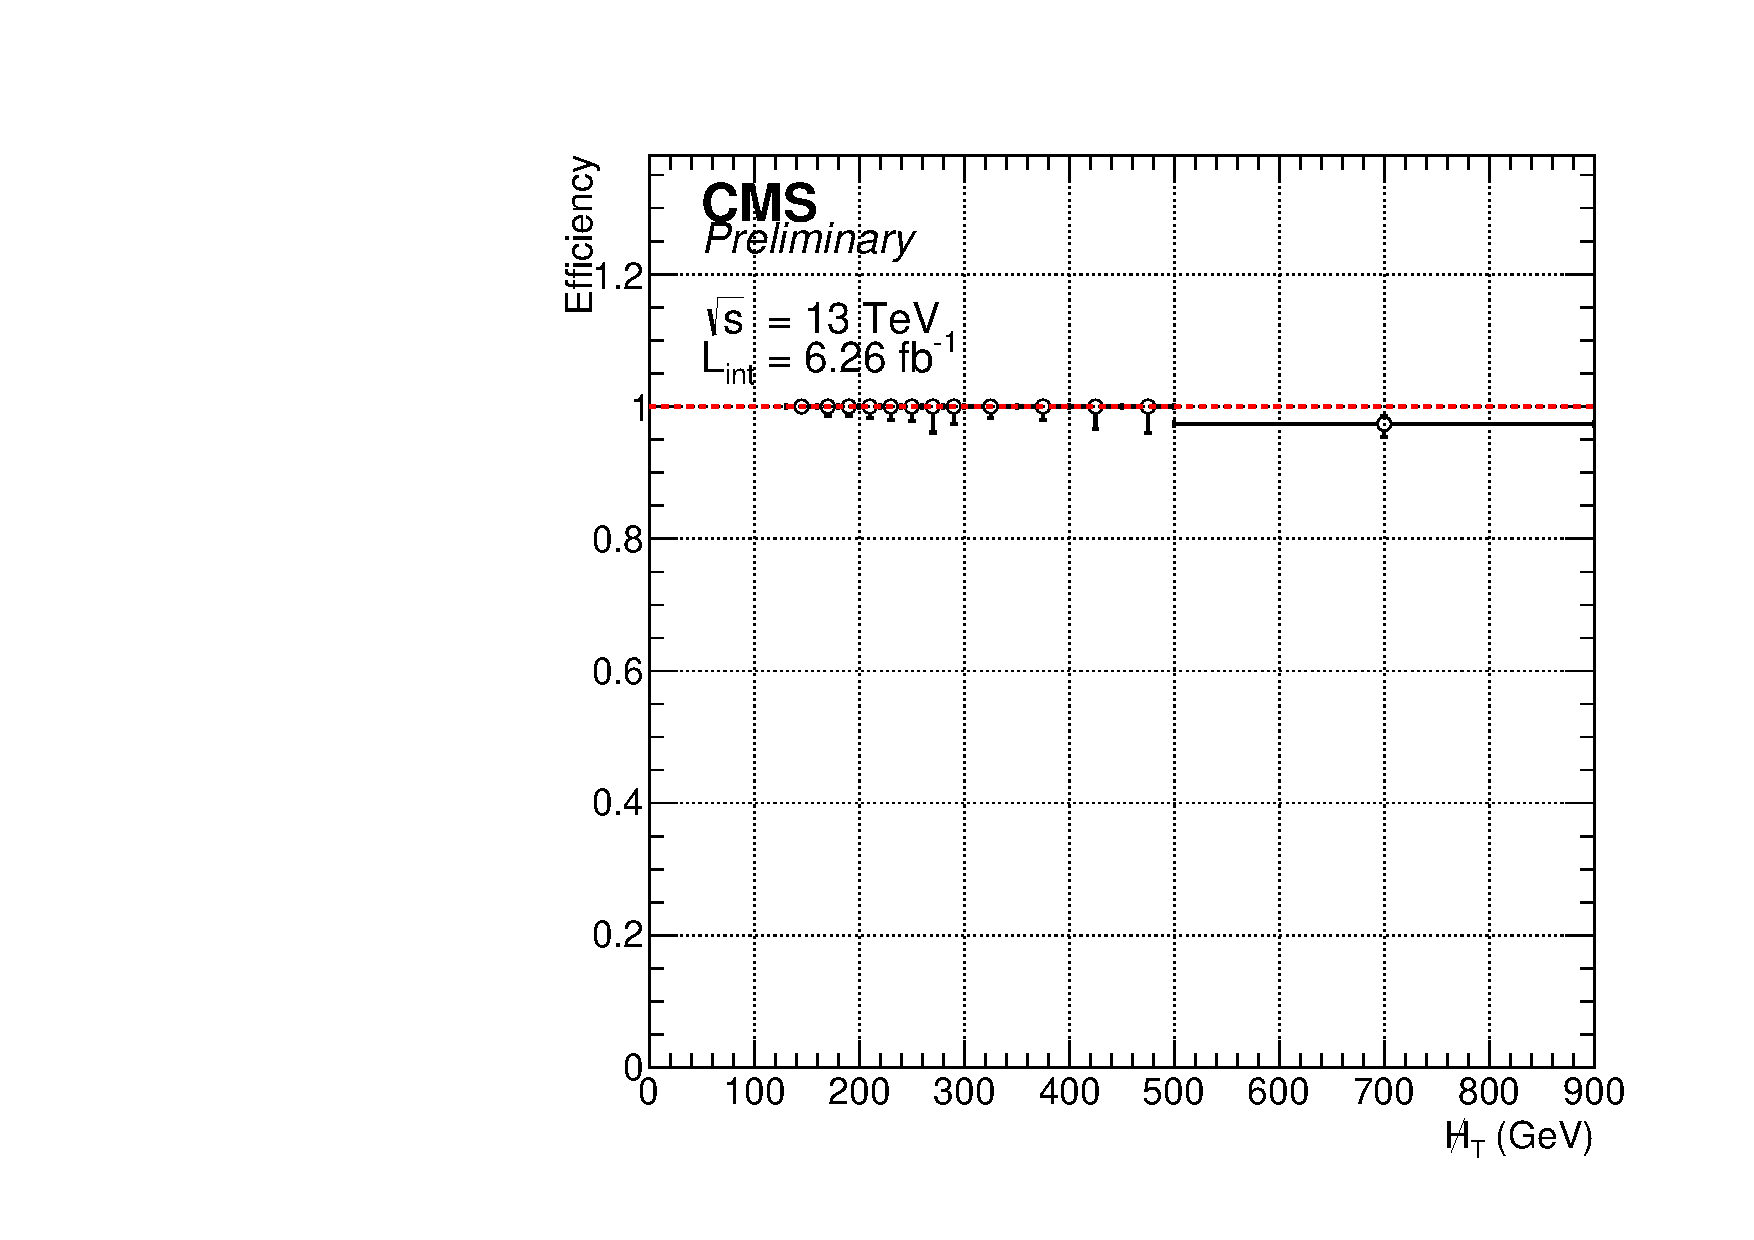
\includegraphics[width=0.4\textwidth]{figures/Trigger/HLT_IsoMu22/HLT_AlphaTHT800MonoAll_MoM_900to999999_mht}} \\
    \caption{Signal trigger efficiency in the \mht dimension measured with a muon sample, for symmetric categories.}
    \label{fig:alphat_turnons_sym}
  \end{center}
\end{figure}

\begin{figure}[h!]
  \begin{center}
    \subfigure[$200 < \scalht < 250$]{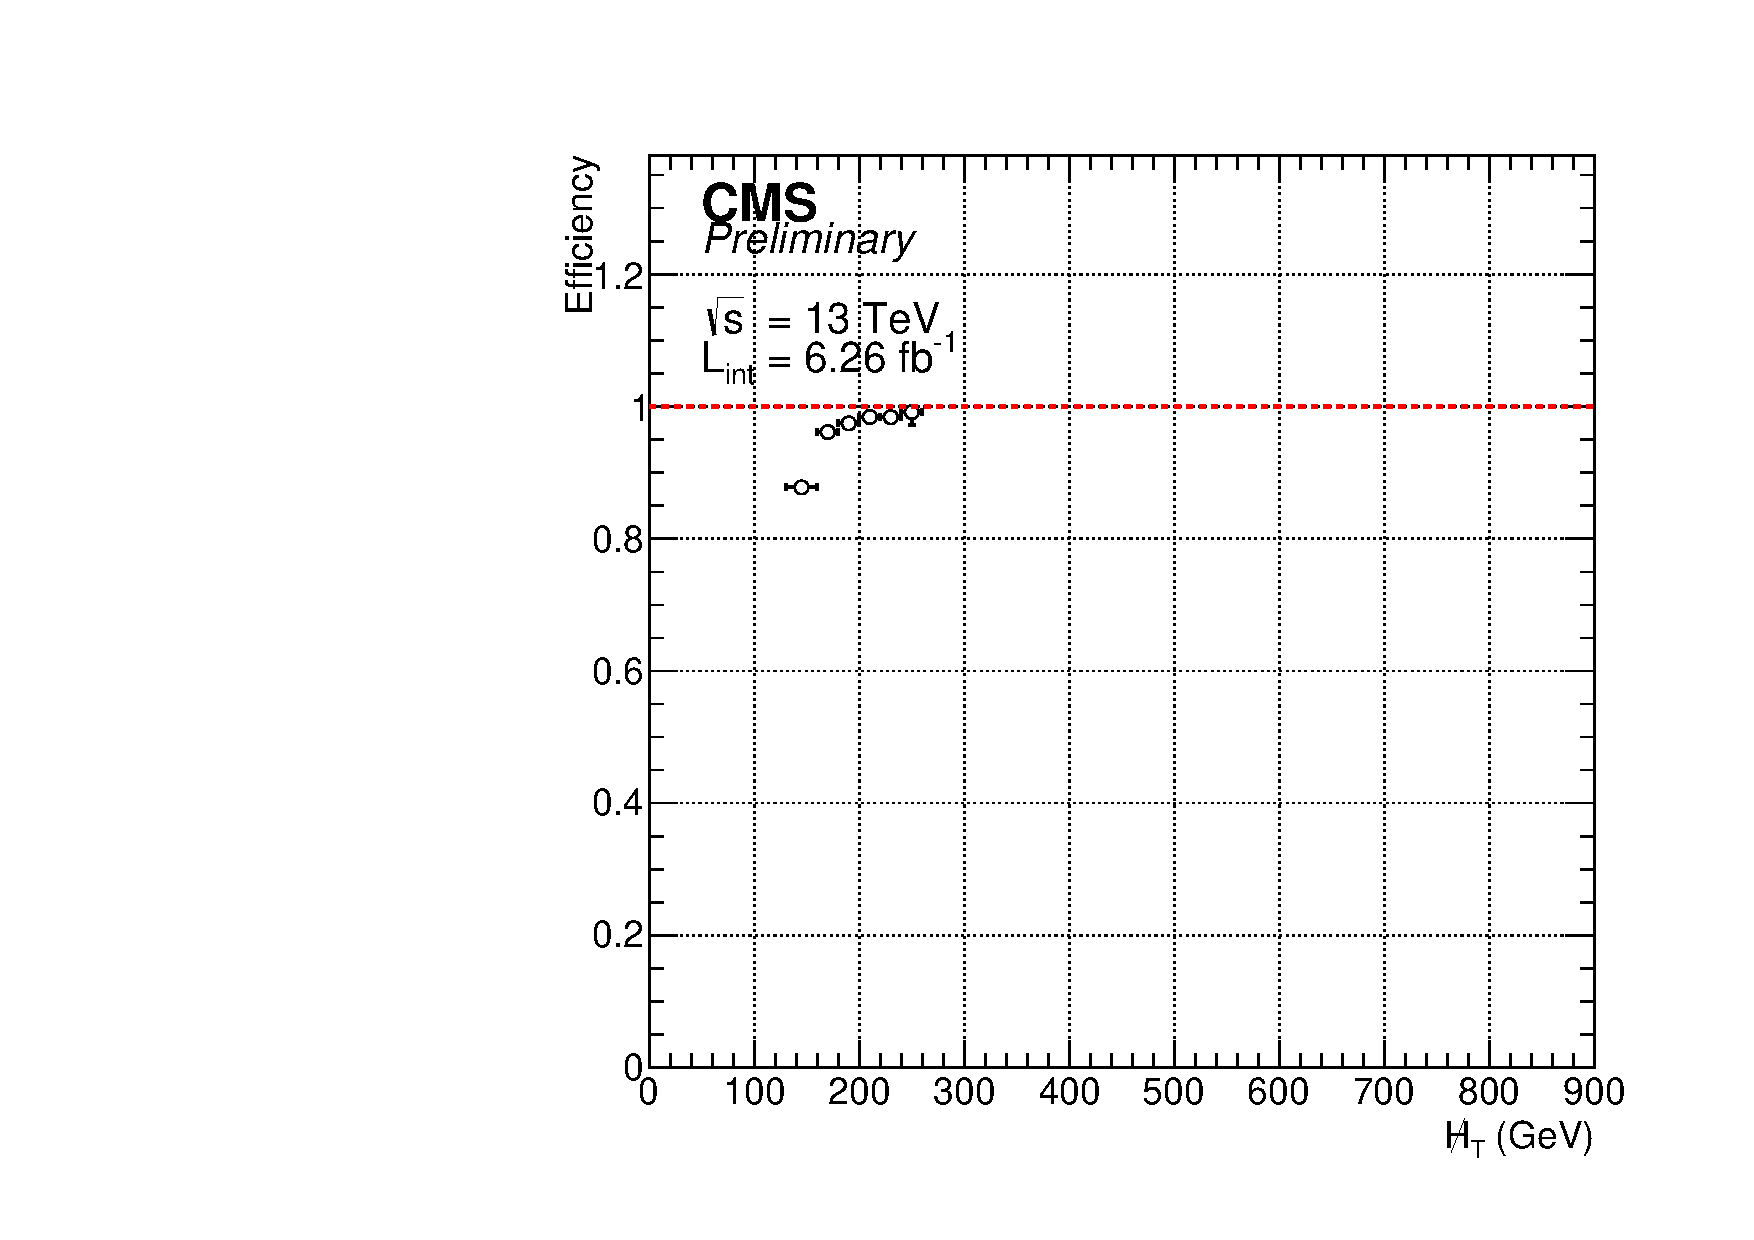
\includegraphics[width=0.4\textwidth]{figures/Trigger/HLT_IsoMu22/HLT_AlphaTMonoAll_MoM_Asym_200to250_mht}} ~~\
    \subfigure[$300 < \scalht < 350$]{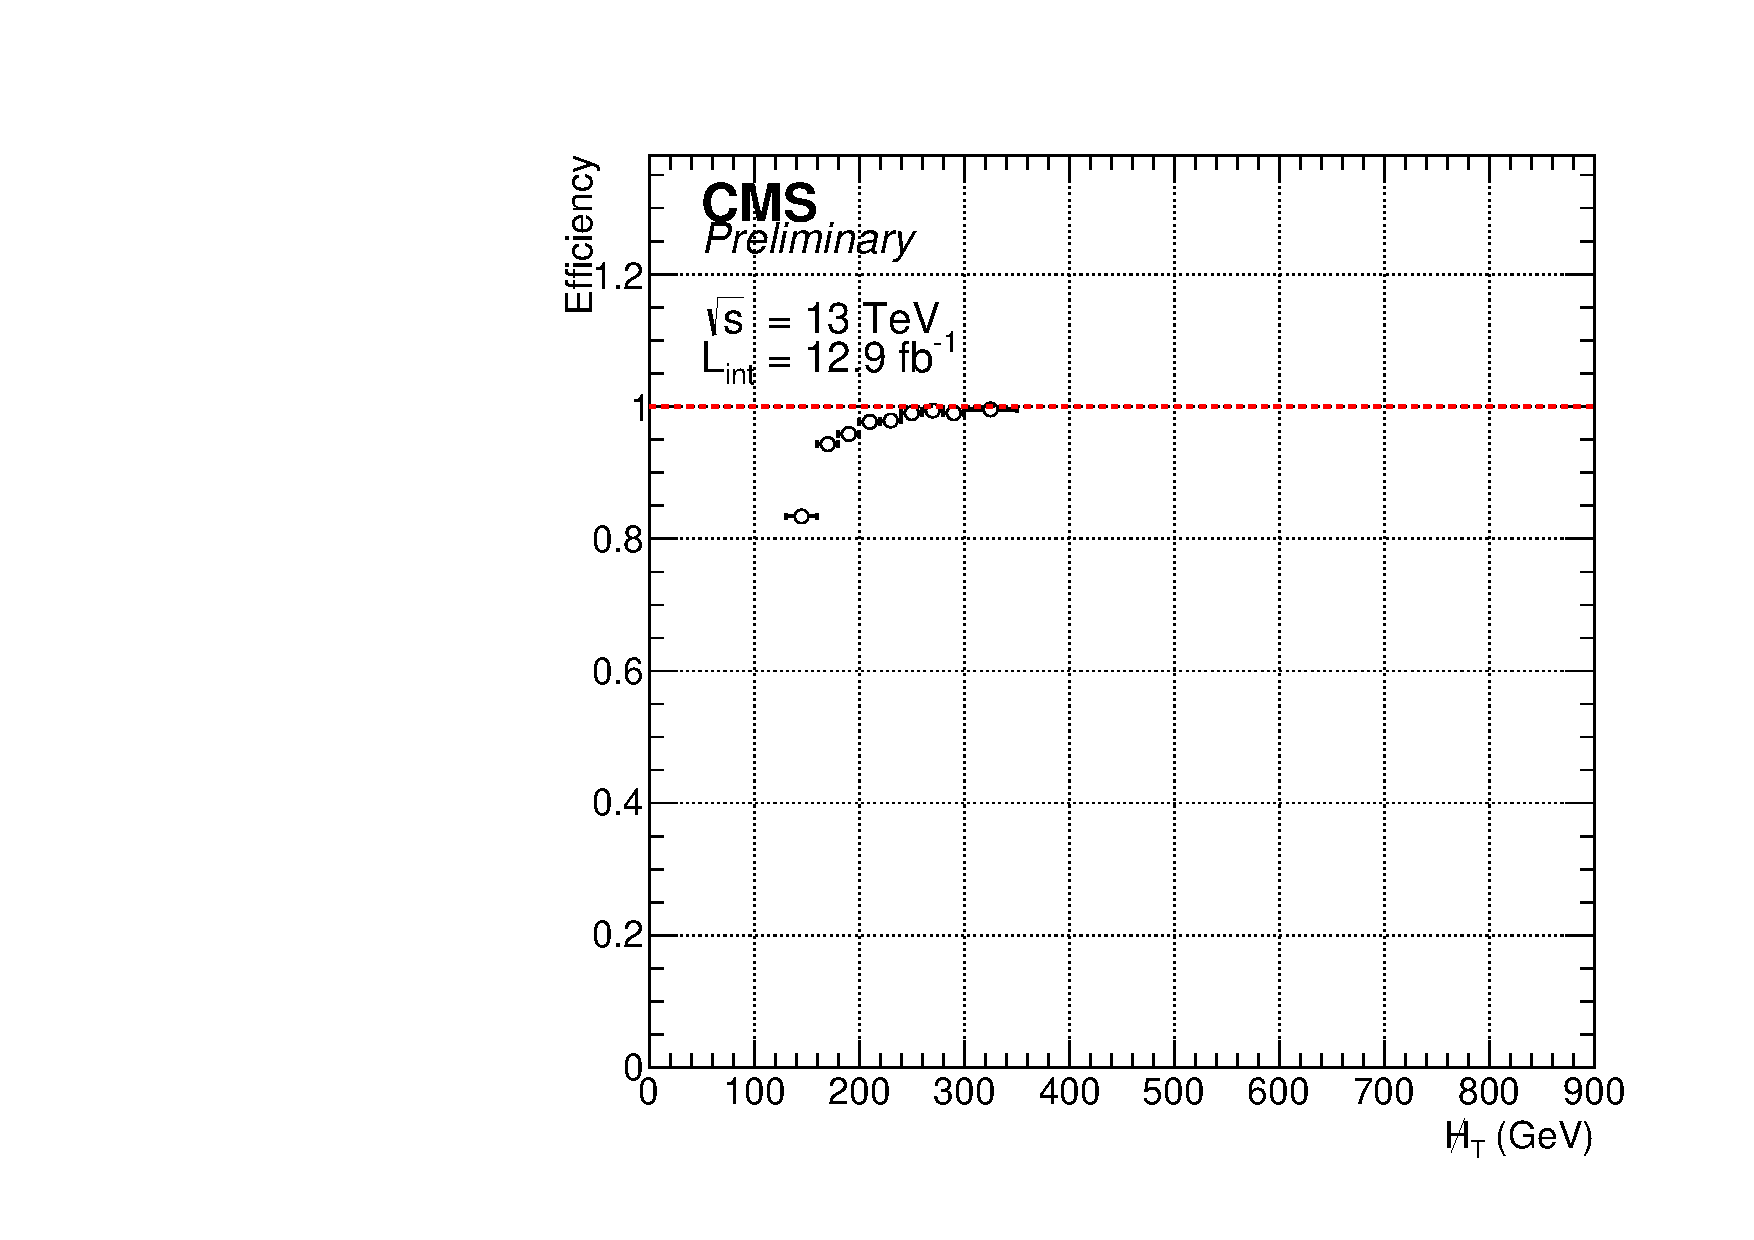
\includegraphics[width=0.4\textwidth]{figures/Trigger/HLT_IsoMu22/HLT_AlphaTMonoAll_MoM_Asym_300to350_mht}} \\
    \subfigure[$400 < \scalht < 600$]{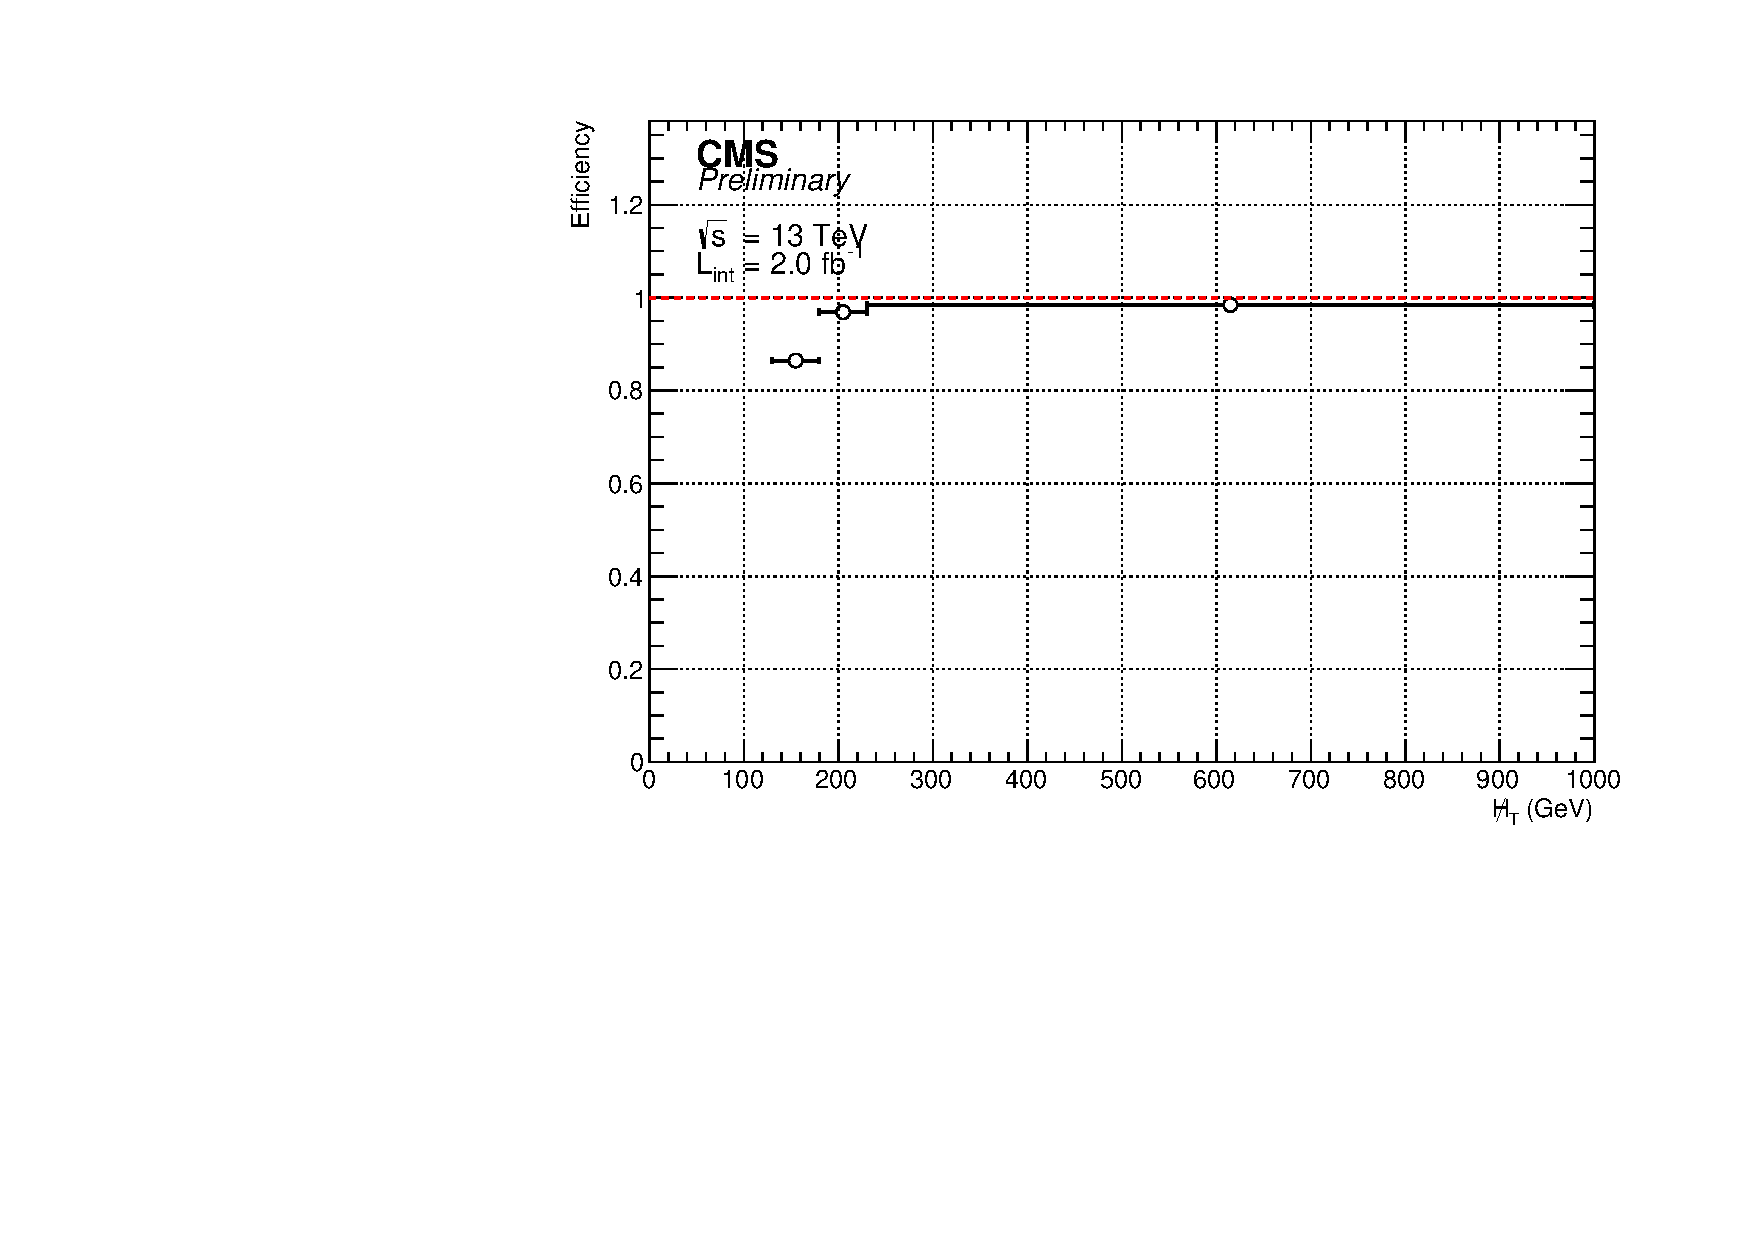
\includegraphics[width=0.4\textwidth]{figures/Trigger/HLT_IsoMu22/HLT_AlphaTMonoAll_MoM_Asym_400to600_mht}} ~~\
    \subfigure[$600 < \scalht < 800$]{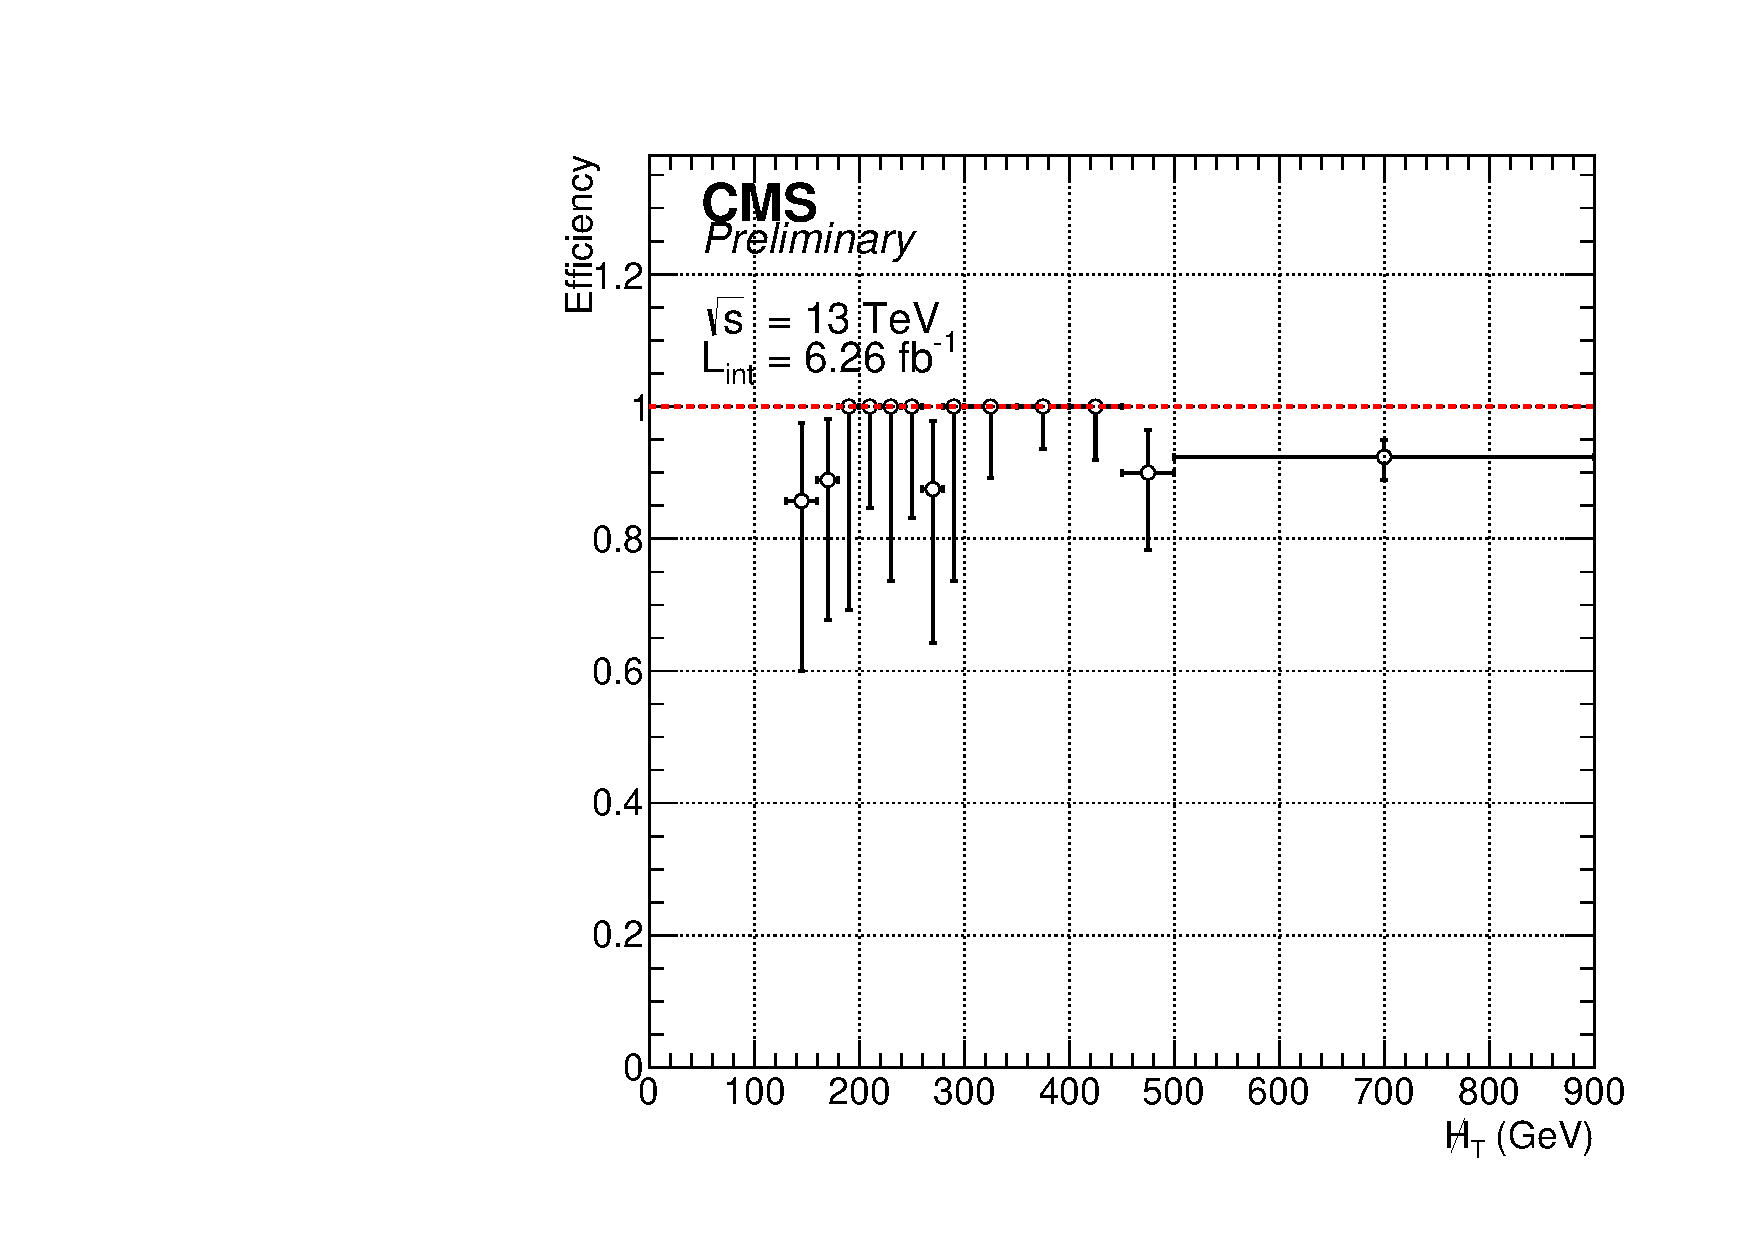
\includegraphics[width=0.4\textwidth]{figures/Trigger/HLT_IsoMu22/HLT_AlphaTMonoAll_MoM_Asym_600to800_mht}} \\
    \caption{Signal trigger efficiency in the \mht dimension measured with a muon sample, for asymmetric categories.}
    \label{fig:alphat_turnons_asym}
  \end{center}
\end{figure}

%\begin{figure}[h!]
%  \begin{center}
%    \subfigure{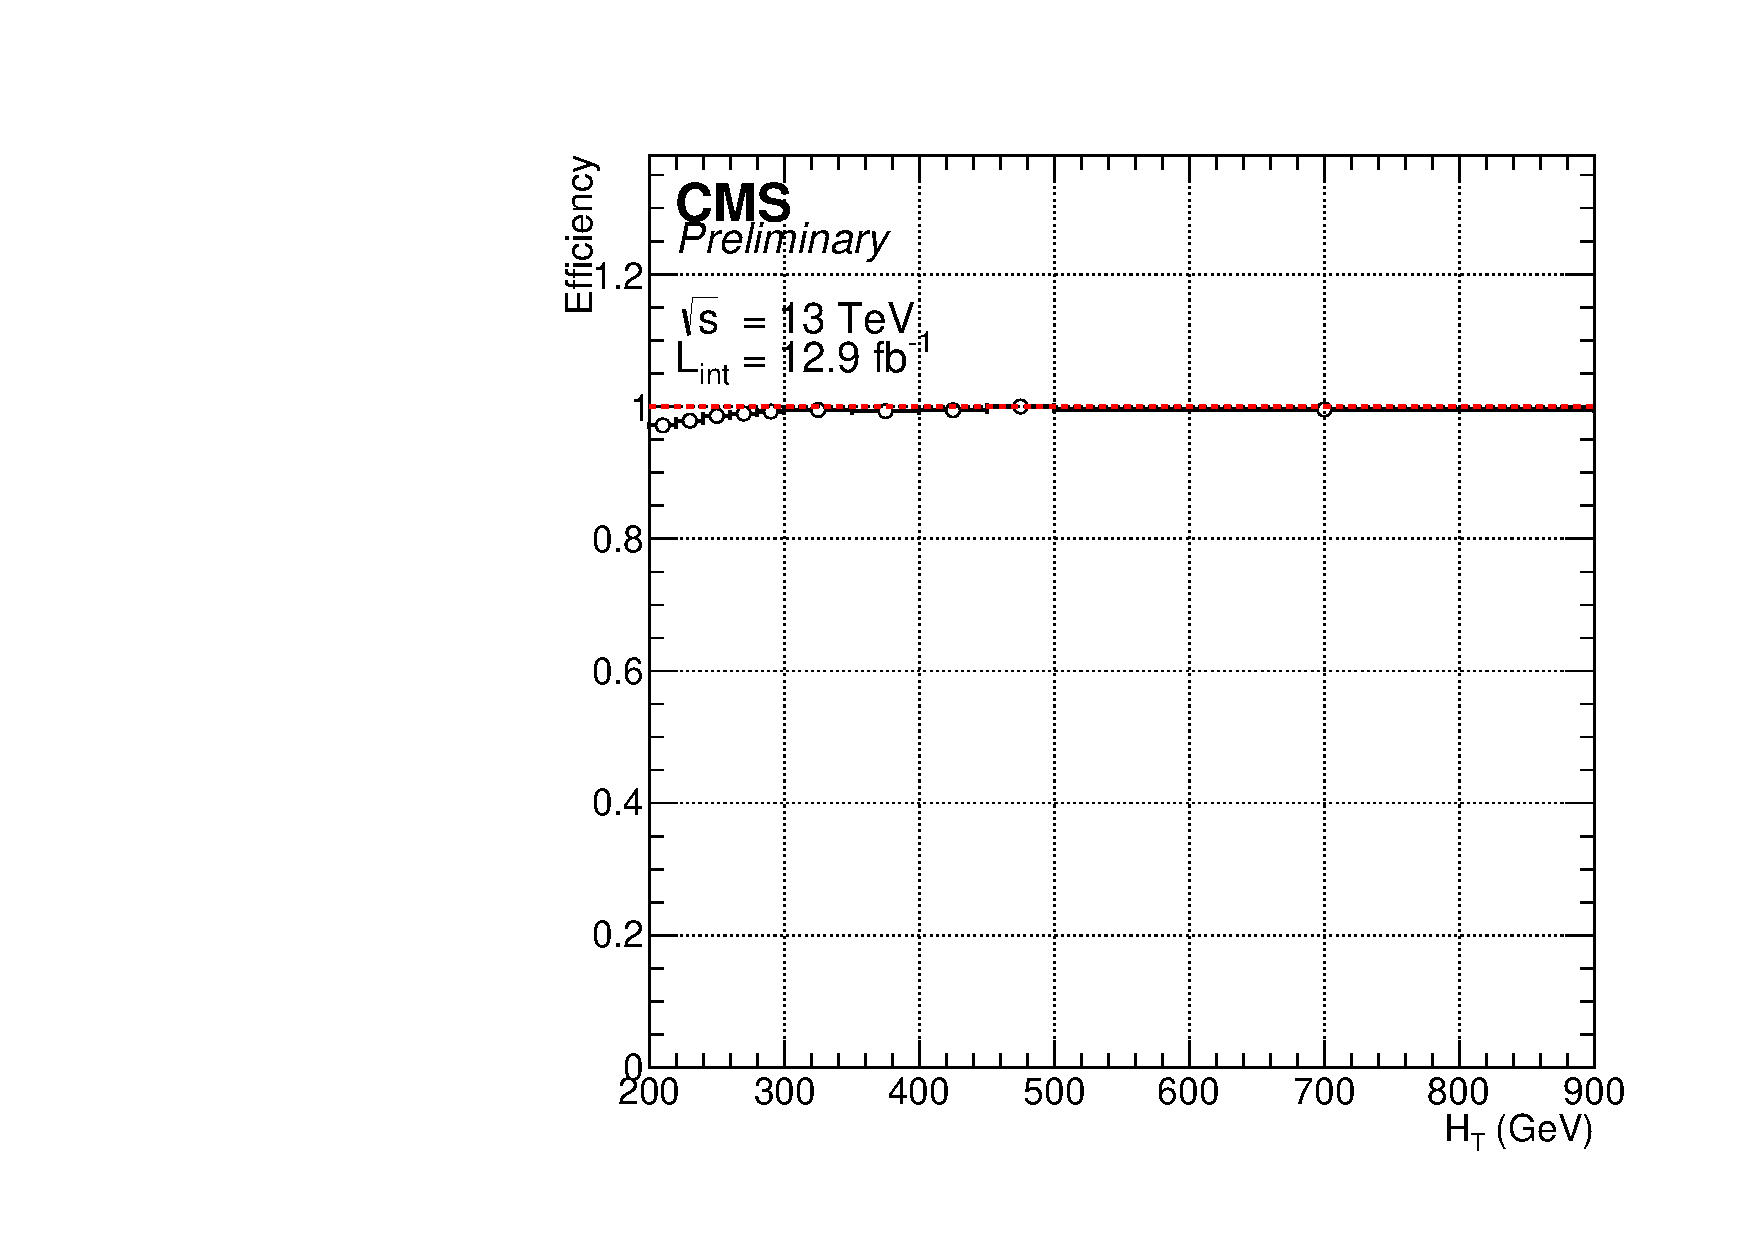
\includegraphics[width=0.5\textwidth]{figures/Trigger/HLT_IsoMu20/HLT_MonoAll_MoM_Mono_MHT0_ht}} \\
%    \caption{Signal trigger efficiency in the \mht$=$\scalht dimension measured with a muon sample, for monojet categories.}
%    \label{fig:alphat_turnons_mono}
%  \end{center}
%\end{figure}



%\newpage

% Control region triggers
\subsection{Control regions\label{sec:control_samples}}
%Prescaled $\scalht$ triggers, \verb!HLT_PFHTXXX!, and a prescaled 
%$\scalht$-$\alphat$ cross-trigger, are utilised in the 
%selection of events for the hadronic control region. Shown 
%in Table~\ref{tab:2015_Hadronic_Control_Triggers} these triggers share the same Level-1 
%seeds and $\scalht$ threshold of the signal cross-triggers and are similarly each mapped 
%to a unique offline bin. The efficiency of these triggers are similarly measured from an electron 
%reference trigger in addition to an independent measurement with the \verb!HLT_Physics! 
%minimum bias trigger.


% TABLE: Hadronic control region
%\begin{table}[h!]
%\topcaption{Hadronic control triggers. }
%\footnotesize
%\centering
%\begin{tabular}{c|cc} 
%\hline
%\hline
%HLT path & \multicolumn{1}{c}{Prescale} \\
%\hline
%\texttt{HLT\_PFHT200} & 3060 \\
%\texttt{HLT\_PFHT250} & 2040 \\
%\texttt{HLT\_PFHT300} & 1020 \\
%\texttt{HLT\_PFHT350} & 180  \\
%\texttt{HLT\_PFHT400} & 120  \\
%\texttt{HLT\_PFHT200\_PFAlphaT0p51} & 175 \\
%\hline
%\hline
%\end{tabular}
%\label{tab:2015_Hadronic_Control_Triggers}
%\end{table}


The non-hadronic control regions are seeded by the lowest-threshold unprescaled 
triggers available in the given run scenario. The 
\mj and \mmj control samples are selected with the logical OR of the \verb!HLT_IsoMu22!
and \verb!HLT_IsoTkMu22! triggers.
The efficiency is measured in data by the muon POG using the tag and probe method,
and corrections are applied to the MC samples as a function of muon \Pt and $\eta$.

The \gj control sample is selected by the OR of the \verb!HLT_Photon175! and
\verb!HLT_ECALHT800! triggers. The efficiency is measured as a function of photon
\Pt for events in the JetHT data set satisfying the \gj control region selection,
and is show in Fig.~\ref{fig:photon_turnons}. The single photon trigger exhibits a decreasing efficiency
with increasing photon \Pt, which is attributed to an H/E cut at Level 1. The inefficiency
can be partly recovered by employing the ECALHT800 trigger. In this way, the 
efficiency above a photon \Pt of 500 GeV is almost 100\%. These efficiencies are used
to correct the MC samples, and a systematic uncertainty with a size of the 
inefficiency is assigned.

\begin{figure}[h!]
  \begin{center}
    \subfigure[$200 < \scalht < 250$]{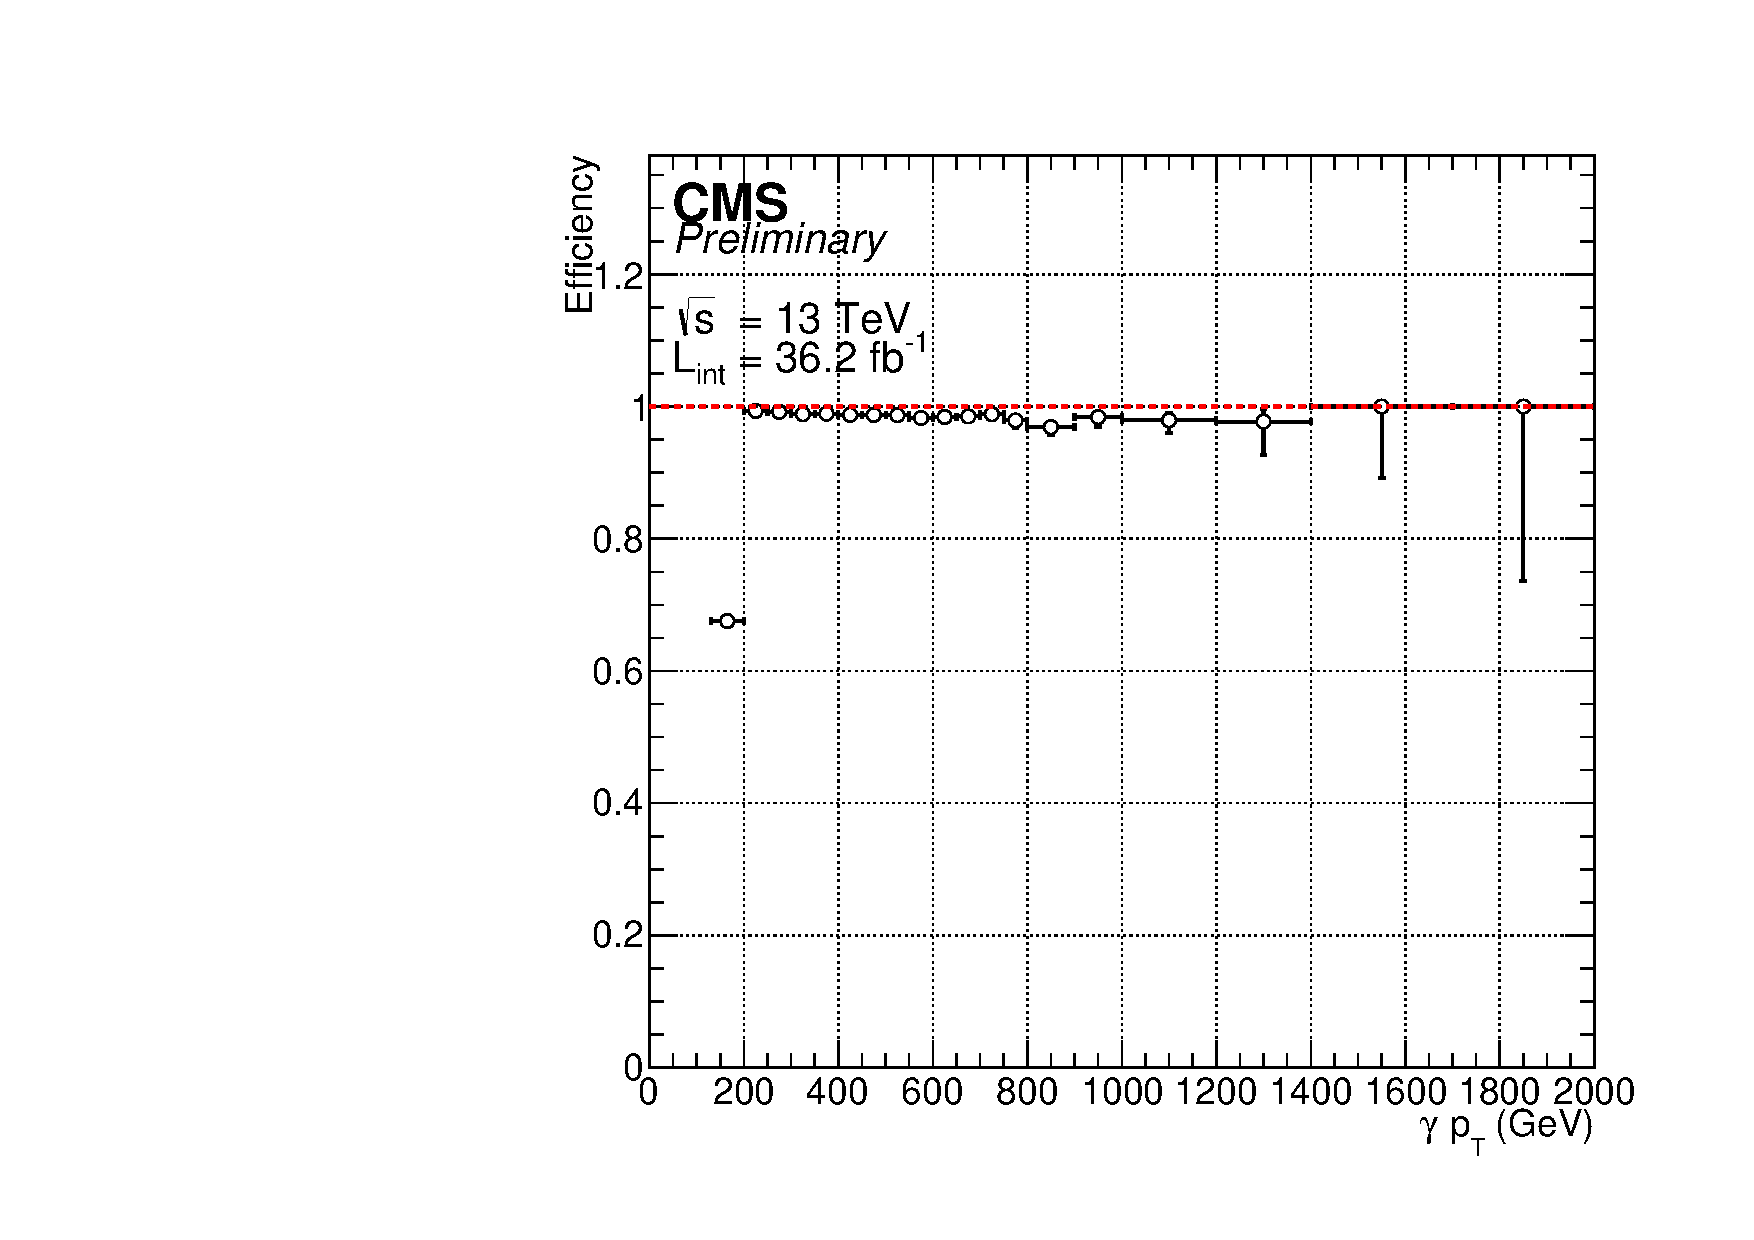
\includegraphics[width=0.5\textwidth]{figures/Trigger/Photon/HLT_Photon175_MoM_all_all_gammapt}} ~~\
    \subfigure[$300 < \scalht < 350$]{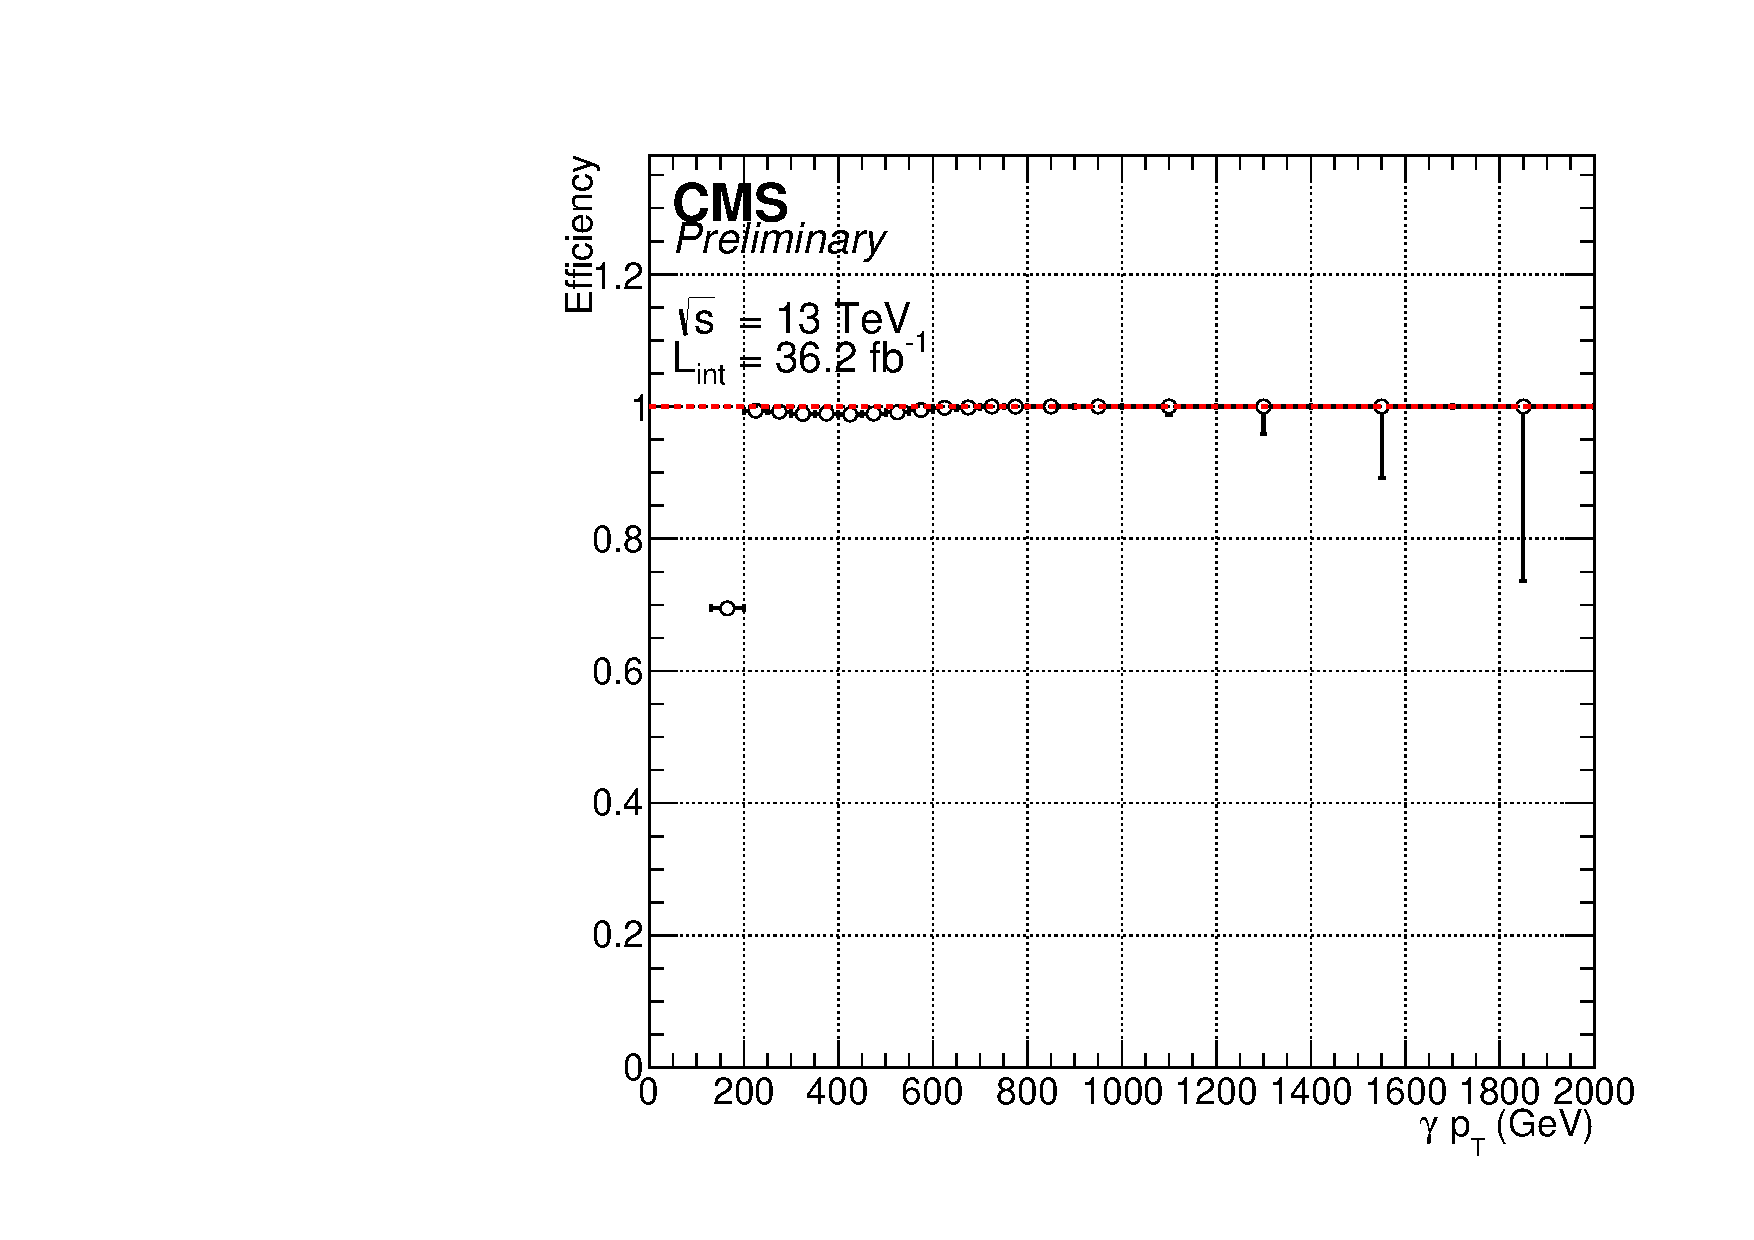
\includegraphics[width=0.5\textwidth]{figures/Trigger/Photon/HLT_PhotonECALHT800_MoM_all_all_gammapt}} \\
    \caption{Trigger efficiency as a function of photon \Pt for Photon175 (left) and Photon175 OR ECALHT800 (right), measured with events in the JetHT data set passing the \gj control region selection.}
    \label{fig:photon_turnons}
  \end{center}
\end{figure}


%The \ej and \eej control samples may be seeded by the \verb!HLT_Ele23_eta2p1_WPLoose_Gsf! trigger.

%The efficiency of the control triggers is measured with data-driven methods
%(provided by the relevant POG). The tag and probe method is used in the measurement of
%efficiencies of the muon and electron triggers and a loose photon reference trigger 
%is utilised in the measurement of the photon trigger efficiency. For the muon control 
%regions the emulated trigger bit in MC is used to simulate 
%the trigger, and efficiency corrections provided by the POG are applied. 
%An offline \Pt requirement of 200\GeV is made on the photon
%to ensure it is in the efficiency plateau of the trigger.



%%____________________________________________________________________________||

%%____________________________________________________________________________||
\section{Physics objects}
\label{sec:objects}
The definitions of the physics objects used in this analysis follow the recommendations of the various Physics Object Groups (POGs). 
During data taking these recommendations are subject to change and will be be updated if necessary.

\subsection{Jets}
\label{sec:jetreco}
Jets are defined as sets of particle-flow (PF) candidates clustered by the
anti-$k_{T}$ jet clustering algorithm \cite{Cacciari:2008gp} with a distance parameter of 0.4
(PFJets). Charged Hadron Subtraction (CHS) is applied, i.e., charged
hadrons that can be traced back to pileup vertices are not clustered.
The four-momenta of jets are initially defined as the four-vector sum of
the four-momenta of the constituent particle-flow candidates and then
scaled by the jet energy correction factors designated as L1FastJet,
L2Relative, and L3Absolute \cite{Chatrchyan:2011ds}.

The ``loose'' working point Jet-Id selection criteria is chosen. 
The cuts are listed in Tab.~\ref{tab:loose-jet-id}. 
In addition, a dedicated selection is applied to reject ``beam halo'' candidate events, 
as described in Section~\ref{sec:had-signal}.

\begin{table}[ht!]
  \caption{The ``loose'' jet ID requirements. \label{tab:loose-jet-id}}
  \centering
  \begin{tabular}{ ccc }
    \hline
    \hline
    Variable & cut & notes \\ \hline
    \multicolumn{3}{c}{$-3.0 < \eta_{\mathrm{jet}} < 3.0$} \\ \hline    
    Neutral Hadron Fraction & $<0.99$ & - \\
    Neutral EM Fraction & $<0.99$ & - \\
    Number of constituents & $>1$ & - \\
    Charged Hadron Fraction & $>0$ & only for $|\eta_{\mathrm{jet}}| < 2.4$ \\
    Charged Multiplicity & $>0$ & only for $|\eta_{\mathrm{jet}}| < 2.4$ \\
    Charged EM Fraction & $<0.99$ & only for $|\eta_{\mathrm{jet}}| < 2.4$ \\ \hline
    \multicolumn{3}{c}{$|\eta_{\mathrm{jet}}| > 3.0$} \\ \hline        
    Neutral EM Fraction & $<0.90$ & - \\
    Number of Neutral Particles & $>10$ & - \\
    \hline
    \hline
  \end{tabular}
\end{table}

\subsection{b-tagged jets}
\label{sec:btags}
Jets originating from bottom quarks are identified through vertices
that are displaced with respect to the primary interaction
\cite{Chatrchyan:2012jua}.  The algorithm used to tag b-jets is the
Combined Secondary Vertex tagger V2, with the ``medium'' working
point, which is achieved by requiring a cut of $>$ 0.800 on the
algorithm discriminator variable.  This results in a gluon/light-quark
mis-tag rate of $\sim$1 \% (where ``light'' means $u$, $d$ and $s$
quarks), a charm-quark mis-tag rate of $\sim$10 \% and a b-quark b-tag
efficiency of about 60 \%. 

Some validation studies used by the analysis make use of the ``loose''
and ``tight'' working points, which are defined by the thresholds
requirements of 0.460 and 0.935 on the discriminator variable. These
requirements yield light-flavour mistag probabilities of $\sim$10 and
$\sim$0.1\%, respectively.


\subsection{Muons}
\label{sec:muon-id}
Muons are selected in the \mj and \mmj control regions using the ``tight'' working point 
definition of the recommended identification algorithm from the Muon POG. 
Muons are also required to be well isolated, i.e. with a low activity in the vicinity of their track. 
The transverse momenta of PF neutral and charged candidates, as well as photons, lying within a cone around the lepton are summed. 
The relative combined isolation $I^{rel}_{comb}$ is then defined as 
the ratio of this scalar sum to the transverse momentum of the lepton
candidate. Additionally, $\rho\times A_{eff}$ corrections are applied to
remove the effects of pileup.
Muons are defined to be isolated if they fulfill the criterium $I^{rel}_{comb} < 0.15$. 

For the purpose of vetoing muons in the signal region, the ``loose'' working point 
is used, which provides $\sim$ 98 $\%$ efficiency. 
In the hadronic signal region a variable cone size for the isolation is used, which is referred to as ``mini-isolation''. 
This isolation algorithm helps in recovering some efficiency in the lepton selection for boosted topology of top quark decays, 
in which the muon's track may be found close to the jet activity due to the boost of the parent top. 
Therefore, the cone size used for the calculation of the lepton isolation is reduced as a function of 
the lepton \Pt, as follows: $R=0.2$ for $\Pt_{\ell}\leq50\gev$,
$R=10\gev/\Pt_{\ell}$ for $50 \gev < \Pt_{\ell} < 200\gev$ and $R=0.05$ for $\Pt_{\ell} > 200 \gev$.
In the signal region, identified muons with mini-isolation satisfying $I^{rel}_{comb} < 0.2$ are vetoed.


\subsection{Photons}
\label{sec:photon-id}
Photons are identified according to the ``tight'' working point definition ($\sim$ 71 $\%$ efficiency) 
of the simple cut-based photon identification algorithm \cite{photon-id} 
and required to be well isolated. 
A PF-based isolation is used with a cone size $\Delta R$ $<$ 0.3 and
$\rho\times A_{eff}$ corrections are applied to remove the effects of pileup \cite{pf-photon}. 
Table \ref{tab:photon-id-gamma} summarises the identification and isolation selection used. 

Photons are vetoed in the definition of the hadronic signal region and
muon control regions, as described in Sec.~\ref{sec:preSelection},
while a control region with one photon (``\gj'') is defined for the
purpose of the background estimation, as described in
Sec.~\ref{subsec:photoncontrolSelection}.


\begin{table}[ht!]
  \caption{Photon identification selection.\label{tab:photon-id-gamma}}
  \centering
  \footnotesize
  \begin{tabular}{ ccc }
    \hline
    \hline
    Categories & \multicolumn{2}{c}{Barrel}   \\
    Working point  & Tight & Loose \\
    \hline
    Conversion safe electron veto & Yes & Yes  \\
    Single Tower H/E              & 0.05 & 0.05  \\
    $\sigma_{i\eta i\eta}$        & 0.0100 & 0.0102 \\
    PF charged hadron isolation   & 0.76 & 3.32  \\
    PF neutral hadron isolation   & 0.97 + 0.014 $\times$ $p_{\mathrm{T},\gamma}$ + 0.000019 $\times$ $p_{\mathrm{T},\gamma}^{2}$ & 1.92 + 0.014 $\times$ $p_{\mathrm{T},\gamma}$ + 0.000019 $\times$ $p_{\mathrm{T},\gamma}^{2}$  \\
    PF photon isolation           & 0.08 + 0.0053 $\times$ $p_{\mathrm{T},\gamma}$ & 0.81 + 0.0053 $\times$ $p_{\mathrm{T},\gamma}$ \\
    \hline
    \hline
    Categories & \multicolumn{2}{c}{Endcap}   \\
    Working point  & Tight & Loose \\
    \hline
    Conversion safe electron veto & Yes & Yes  \\
    Single Tower H/E              & 0.05 & 0.05  \\
    $\sigma_{i\eta i\eta}$        & 0.0268 & 0.0274 \\
    PF charged hadron isolation   & 0.56 & 1.97  \\
    PF neutral hadron isolation   & 2.09 + 0.014 $\times$ $p_{\mathrm{T},\gamma}$ + 0.000025 $\times$ $p_{\mathrm{T},\gamma}^{2}$ & 11.86 + 0.014 $\times$ $p_{\mathrm{T},\gamma}$ + 0.000025 $\times$ $p_{\mathrm{T},\gamma}^{2}$ \\
    PF photon isolation           &  0.16 + 0.0034 $\times$ $p_{\mathrm{T},\gamma}$ & 0.83 + 0.0034 $\times$ $p_{\mathrm{T},\gamma}$ \\
    \hline
    \hline
  \end{tabular}
  \end{table}


\subsection{Electrons}
\label{sec:electron-id}
In order to veto electrons in the hadronic signal region and the muon
and photon control regions, the ``loose'' working point definition
($\sim$ 90 $\%$ efficiency) of the cut-based electron identification
\cite{electron-id} is used.  Electrons are also require required to be
isolated.  Similar to muons, in the hadronic signal regions a PF-based
isolation \cite{pf-photon} is used with a cone size determined by the
mini isolation algorithm (see Sec.~\ref{sec:muon-id}) and $\rho\times
A_{eff}$ corrections are applied to remove the effects of pileup.
Isolated electrons are defined by $I^{rel}_{comb} < 0.1$.

Table \ref{tab:ele-id} summarises the identification 
selection used. 

\begin{table}[h!]
  \caption{Electron identification (``tight'' working point).\label{tab:ele-id}}
  \centering
  \footnotesize
  \begin{tabular}{ lcc }
    \hline
    \hline
    Categories                                               & Barrel    & EndCap    \\
    \hline
    $\Delta \eta_{In}$                                       & 0.0105   & 0.00814  \\
    $\Delta \phi_{In}$                                       & 0.115    & 0.182  \\
    $\sigma_{i\eta i\eta}$                                   & 0.0103    & 0.0301  \\
    H/E                                                      & 0.104    & 0.0897   \\
    d0 (vtx)                                                 & 0.0261    & 0.118  \\
    dZ (vtx)                                                 & 0.041    & 0.822  \\
    $\lvert(1/E_{\textrm{ECAL}} - 1/p_{\textrm{trk}})\rvert$ & 0.102     & 0.126  \\
    Missing hits (inner tracker)                             & 2         & 1         \\
    Conversion veto                                          & yes       & yes   \\
    \hline
    \hline
  \end{tabular}
  \end{table}


\subsection{Single isolated tracks}
\label{sec:SIT}
A single isolated track (SIT) can be used to identify W bosons through their leptonic decays: 
W $\rightarrow$ $\mu \nu$, W $\rightarrow$ $e\nu$, and W $\rightarrow$ $\tau$($\rightarrow l$) $\nu$. 
Single prong decays of the tau lepton can also be identified: W $\rightarrow$ $\tau$ ($\rightarrow$ h$^{\pm}$ + n$\pi^{0}$) $\nu$. 
A single isolated track comprises a charged PF candidate with $\Pt > 10 \gev$, $\Delta z(\mathrm{track}, \mathrm{PV}) < 0.05 \, \mathrm{cm}$ 
and with a relative isolation smaller than 0.1, where the isolation is determined from the sum 
of the \Pt of the charged PF candidates within $\Delta R < 0.3$.
%Events in the signal region and all control regions (ignoring the
%selected muons) containing a SIT candidate identified with these
%criteria are vetoed.


\subsection{Missing transverse momentum}
Missing transverse momentum (\met) is defined as the magnitude of the vector sum
of the transverse momentum of all particle-flow candidates in the event.
The Type-I \met correction \cite{Khachatryan:2014gga} is applied, i.e., the transverse momentum of
the particle-flow candidates clustered as jets are replaced with the
transverse momentum of the jets that are scaled by the jet energy
correction factors.

The \met is used in the definition of 
the transverse mass, $M_{T}$, which is in turn used as part of
the selection criteria that define the single muon control sample 
(Sec.~\ref{subsec:mucontrolSelection}), and for the $\mhtmet$ cleaning filter, 
as described in Sec.~\ref{sec:selection}.



%%____________________________________________________________________________||

%____________________________________________________________________________||
\section{Event selection for signal and control regions}
\label{sec:selection}

This section first outlines the set of ``pre-selection'' requirements
that are common to all signal and control regions, before defining the
selection criteria that are specific to each region.

%%____________________________________________________________________________||
\subsection{Pre-selection}
\label{sec:preSelection}

{\bf Removing instrumental sources of ``fake'' \met.} 

A number of beam- and detector-related effects can induce significant
\met. Examples include beam halo, reconstruction failures, spurious
detector noise, or event misreconstruction due to detector
inefficiencies. These events, with large, non-physical values of \met,
are rejected with high efficiency by applying a range of dedicated
vetoes. All ``MET filters'' recommended by the JetMET POG and SUSY PAG
are applied by default in this analysis and listed in Table~\ref{tab:pre-selections}.

{\bf Jet requirements.} 

Jets considered in the analysis are required to satisfy $\PT>40\gev$
and $|\eta|<3.0$. Events containing jets in the forward region that
satisfy the requirements $\PT>40\gev$ and $|\eta|>3.0$ are rejected in
order to control background contributions from SM processes, without
introducing a significant reduction in signal acceptance. The jets
that are selected are used in the calculation of all jet-based
event-level variables, such as \HT, \mht, and \alphat.

Raised $\PT$ thresholds and tighter $\eta$ requirements on the lead jets 
are also required. The lead jet is required to satisfy $\PT > 100\gev$
and $|\eta|<2.5$. This helps to ensure high trigger efficiencies,
but also helps to improve the S/B for a wide
range of models with respect to SM processes, such as V + jets
production. Events are then classified based on the
second leading jet. In the case that a second leading jet satisfies $\PT > 100\gev$ 
events are assigned to a ``symmetric'' \njet category. If the second
jet satisfies $40 < \PT < 100\gev$ events are assigned to an
``asymmetric'' \njet category. Finally, if there is no second leading
jet with $\PT>40\gev$, events are assigned to the ``mono-jet''
category. This categorisation is heavily utilised throughout all the document. \\
The asymmetric and mono-jet categories have been added to
the analysis to help improve acceptance to a range of DM models and compressed
SUSY.

{\bf Event categorisation according to \njet and \nb.} 

Events in the hadronic signal and all control regions (described
below) are categorised identically and according to the number of jets
(\njet) reconstructed in each event and the number of jets identified
as originating from bottom quarks (\nb) in each event. As a baseline,
the resulting sub-samples comprise events containing exactly one, two,
three, four, or at least five jets. These are further split into
``monojet'' (only in the $\njet=1$ case),
``symmetric'' or ``asymmetric'' \njet categories according to the
second leading jet \Pt, as defined above.

Events are also categorised according to the the number of b-tagged
jets (``b-jets''). As a baseline, the sub-samples are defined by
requiring exactly zero, one, two, or at least three b-tagged jets. By
construction, $\nb \leq \njet$. Standard Model background events containing three or more b-tags
typically arise from an additional source of b-jets like 
``gluon splitting'' or from 
mistag of a jet from a light-flavoured parton. 


{\bf \HT,\mht requirements and binning.} 

Events are required to have significant hadronic activity by requiring
$\scalht > 200\GeV$. Despite an increase in both multijet production
cross sections and pileup in Run~2, the lowest \HT threshold is
kept at the same value of the Run~1 analysis~\cite{Chatrchyan:2013lya}
in order to maintain acceptance to DM models or compressed
SUSY. Events in all samples are binned identically, according to the
\HT variable. The choice of binning in \HT is driven primarily by the
trigger strategy employed by the analysis, as described in
Section~\ref{sec:triggers}, and can be summarised as follows: 50\gev
bins in the range $200 < \HT < 400\gev$, 100\gev bins in the range
$400 < \HT < 600\gev$, a 200\gev bin $600<\HT<800\gev$ and a final 
inclusive bin $\HT > 800\gev$.

Events are also required to have appreciable missing hadronic energy
by requiring $\mht>130\gev$. This ensures that all events used within
the analysis have a degree of missing energy similar to that required
in the signal region via an \alphat cut. This is outlined in
Sec.~\ref{sec:had-signal}. 

The lower threshold of the last (inclusive) \HT bin is not forced to
$800\gev$, it is instead determined
independently for each (\njet,\nb) event category and is chosen to
always align with one of the ``default'' boundaries defined above. The
metric for choosing the final bin threshold is based on the number of
events in the corresponding event category and \HT bin of the data
control samples. This ensures that all bins in the data control
samples are sufficiently populated to ensure a statistically
significant prediction in each of the corresponding signal region
bins. Currently, this is achieved by requiring at least $10$ predicted
events in each \HT and \njet category of the control regions
along with the requirement that there is at least one observed
event per \nb category. If this is not the case, events from high \HT bins are combined
into a single inclusive bin that satisfies this metric. This metric
ensures that there are sufficient events in the control samples
to probe for potential systematic effects with closure tests between
simulation and data, as described in Sec.~\ref{sec:systematics}.

\begin{table}[h!]
  \topcaption{Summary of the pre-selection criteria.}
  \label{tab:pre-selections}
  \centering
  \footnotesize
  \begin{tabular}{ ll }
    \hline
    \hline
    Selection                     & Requirement                                                                          \\
    \hline
    ``MET filters''               & Primary Vertex, CSC Beam Halo, HBHE Noise and Isolation, ECAL Endcap SC Noise        \\
    Jet acceptance                & $\PT > 40\gev$, $|\eta| < 3$                                                         \\
%    \njet                         & $\geq2$                                                                \\
    Lead jet acceptance           & $\PT > 100\gev$, $|\eta| <    2.5$                                     \\
    Second jet acceptance         & $\PT > 100\gev$ \texttt{OR} $40 < \PT < 100\gev$                       \\
    Loosest \HT requirement       & $\HT > 200\gev$                                                        \\
    Loosest \mht requirement      & $>130\gev$                                                     \\  
    Baseline \HT binning          & 200--250, 250--300, 300--350, 350--400, 400--500, 500--600, 600--800, $>$800\gev \\
    Baseline \njet multiplicities & 1 (mono-jet), 2, 3, 4, $\geq$5 (both symmetric and asymmetric)                       \\
    Baseline \nb multiplicities   & 0, 1, 2, $\geq3$ ($\nb \leq \njet$)                                    \\
    \hline
    \hline
  \end{tabular}
\end{table}

{\bf Summary of pre-selection requirements.} 

Table~\ref{tab:pre-selections} summarises the pre-selection
requirements and default categorisation and binning scheme. The
threshold of the final \HT bin per (\njet,\nb) category is summarised
in Table~\ref{tab:binning-3fb}. An identical scheme is used for the
signal region and all control regions. No extrapolation is performed
in the variables \njet, \nb, and \HT in this analysis. For each of the
signal and control regions, thirty event categories are considered,
each with up to seven bins in \HT, assuming an integrated luminosity
of 2.1\ifb. 

\begin{table}[h!]
  \caption{Threshold (GeV) of the final \HT bin as a function of event
    category (\njet,\nb), which is always aligned with respect
    to one of the baseline boundaries (motivated primarily by the trigger) of
    200, 250, 300, 350, 400, 600, 800\gev. 
    %This is the projected choice for 3\fbinv.
    }
  \label{tab:binning-3fb}
  \centering
  \footnotesize
  \hspace*{-1cm}\begin{tabular}{ l|cc|ccc|cccc|cccc|cccc }
    \hline
    \hline
    \njet      & \multicolumn{2}{c|}{1} & \multicolumn{3}{c|}{2} & \multicolumn{4}{c|}{3} & \multicolumn{4}{c|}{4} & \multicolumn{4}{c}{$\geq5$} \\ 
    \nb        & 0   & 1   & 0   & 1   & 2   & 0   & 1   & 2   & 3   & 0   & 1   & 2   & $\geq3$ & 0   & 1   & 2   & $\geq3$ \\
    \hline
    Symmetric  & 600 & 500 & 800 & 800 & 600 & 800 & 800 & 800 & 400 & 800 & 800 & 800 & 800     & 800 & 800 & 800 & 800     \\
    Asymmetric & -   & -   & 600 & 500 & 400 & 600 & 600 & 500 & 300 & 600 & 600 & 600 & 400     & 600 & 600 & 600 & 500     \\
    \hline
    \hline
  \end{tabular}
\end{table}


\subsection{Lepton and photon vetoes \label{sec:vetoes}}

To select a sample of events in the hadronic final state and to
suppress SM processes with genuine \met from neutrinos, events
containing an isolated electron with $\pt > 10\GeV$ and $|\eta| < 2.5$
or an isolated muon with $\pt > 10\GeV$ and $|\eta| < 2.5$ are
vetoed. Further, to reduce the ``lost leptons'' backgrounds from \wj
and \ttbar, events containing single isolated tracks with $\pt >
10\GeV$ and $|\eta| < 2.5$, as defined in Sec.~\ref{sec:objects},
are vetoed as part of the signal region selection criteria. In the
case of the single and di-lepton control samples, a further
requirement is made such that events are not vetoed due to the
presence of a track from the well identified leptons, by requiring
$\Delta R(\textrm{track},\textrm{lepton}) > 0.02$.

Finally, to select a purely hadronic topology and to allow for a
orthogonal control region, events are vetoed in which an isolated photon
with $\pt > 25\GeV$ and $|\eta| < 2.5$ is identified.

\subsection{The hadronic signal region}
\label{sec:had-signal}

The lepton and photon vetoes are applied to select hadronic final
states. All pre-selection criteria are also applied. Following these
selections, the multijet background from QCD is still several orders
of magnitude larger than the typical signal expected from SUSY.

{\bf \HT-dependent \alphat requirements.}

Background events from multijet production populate the region
$\alphat \lesssim 0.5$ and therefore can be rejected with very high
efficiency by requiring an appropriate cut on \alphat. 

A useful approximate conversion between \alphat and \mht can be
obtained by calculating \alphat, as described by Eq.~\ref{eq:alphat3}, 
while forcing $\dht = 0\gev$,. Hence, using this metric, the
dependence of the \alphat requirement as a function of the \HT bin can
be determined such that the effective requirement on \mht is
comparable, \ie roughly constant, across all \HT bins. The values
typically fall in the range $\sim110 < \mht < \sim160\gev$. This
approximate levelling of the ``effective'' \mht threshold implies
increasingly tighter requirements against instrumental effects versus
\HT, while maximising signal
acceptance. Table~\ref{tab:alphat-thresholds} summarises the 
\alphat thresholds and corresponding ``effective'' \mht thresholds for
each \HT bin. The \alphat threshold is dependent only on \HT and not
on \njet nor \nb that are used to define the event categories.

\begin{table}[h!]
  \caption{\alphat and corresponding ``effective'' \mht (GeV) thresholds versus
    lower bound of \scalht bin. For all \HT bins satisfying $\HT > 800
    \gev$, the direct requirement of $\mht > 130\gev$ is imposed rather
    than a requirement on \alphat. No \alphat requirement is imposed in the
    monojet bins.}
  \label{tab:alphat-thresholds}
  \centering
  \footnotesize
  \begin{tabular}{ lcccccccc }
    \hline
    \hline
    \scalht            & 200       & 250       & 300       & 350       & 400       & 500       & 600       \\
    \hline                                                                                     
    \alphat threshold  & 0.65      & 0.60      & 0.55      & 0.53      & 0.52      & 0.52      & 0.52      \\
    ``Effective'' \mht & $\sim$128 & $\sim$138 & $\sim$125 & $\sim$123 & $\sim$110 & $\sim$138 & $\sim$162 \\
    \hline
    \hline
  \end{tabular}
\end{table}

For all signal region bins satisfying $\HT > 800\gev$  no \alphat
threshold is required, which removes the inefficiencies of this
variable for high jet multiplicity events. Instead, the following
$\mht >130\gev$ requirement helps to control the multijet background
along with the imposition of $\bdphi > 0.5$ (described below).

{\bf \bdphi requirement.} 

Further, an additional powerful variable \bdphi is used to suppress
multijet contamination due to both instrumental effects and
semi-leptonic heavy-flavour decays with genuine \met in the final
state. The variable is determined as follows. The jet-based estimate
of the missing transverse energy, ${\mhtvec}$, is recomputed while
ignoring one of the reconstructed jets (the ``test'' jet). The
difference in the azimuthal angle between the recomputed $\mhtvec$
and the ``test'' jet is then determined. This process is repeated for
each jet in the event and the minimum of all the azimuthal
differences, \bdphi, is determined. For monojet events, the calculation is 
performed using all jets with $\Pt > 20\gev$. The ``test'' jet whose subtraction
from the calculation $\mhtvec$ yields this minimum value, is
identified as the jet that is most likely to have given rise to the
missing transverse energy in the event. Events with significant \mht
due to instrumental effects or heavy flavour decays populate the
region at $\bdphi$ and so candidate signal event are accepted
only if they satisfy $\bdphi > 0.5$. The use of the \bdphi and \alphat
variables provide an extremely powerful rejection factor against
contamination from multijet events and allow to maintain low jet \PT,
\HT, and \mht thresholds, which in turn maximises signal acceptance
for a large range of DM and SUSY models with final states
characterised by the presence of significant \met.

{\bf $\mht/\met$ cleaning filter.} 

To protect against multiple jets failing the $\Et$ threshold or
falling out of detector acceptance, the jet-based
estimate of the missing transverse energy, \mht, is compared to the
missing transverse energy variable, $\met$, and events with $R_{\rm
  miss}=\mht/\met > 1.25$ are rejected.
  
{\bf Detector dead cell control.}

Masked regions in the ECAL (which amount to about 1\% of the ECAL channel count)
or HCAL, or by missing instrumentation in the barrel-endcap gap, could cause 
severe energy losses. A data-driven method is developed to identify dead cells. The 
procedure is carried out on events that pass a loose selection of one good primary vertex,
$\njet>1$ and $\scalht>150\gev$. For each identified jet with
$\PT > 20 \gev$ in data, the azimuthal angle ($\Delta\phi_{jet}$) between the jet and the 
recomputed ${\mhtvec}$ is determined, in the same way as in the procedure to compute the \bdphi 
variable. The positions of all jets which give $\bdphi < 0.3$ are plotted in
an $\eta-\phi$ map. Subsequently, the positions of all jets with
$\pt>20\gev$ are plotted in a second $\eta-\phi$ map.
These two maps are then divided to form a 2D ratio map, taking the
first map as the numerator and second as the denominator.
Jets pointing to dead cells are likely to give $\bdphi < 0.3$, so the
location of dead cells in $\eta$ and $\phi$ have higher values in this 2D ratio map. 

Figure~\ref{fig:2dRatioMap} is the 2D ratio map made with unblinded signal region with luminosity of 
149.49~$\text{pb}^{-1}$. In the lower left region of the plot, two
areas with significant instrumental effects are clear. To ensure these
effects are filtered out by all cleaning cuts within the analysis, an
$\eta-\phi$ map of all jets with $\pt>20\gev$ and $\bdphi<0.3$ are
plotted after the signal region selection (as described in
Sec.~\ref{sec:had-signal}), shown in
Fig.~\ref{fig:jetMapPostSignalSelection}. The areas with significant
instrumental effects visible in Fig.~\ref{fig:2dRatioMap} do not appear
to remain in Fig.~\ref{fig:jetMapPostSignalSelection}. This implies the current suite of cleaning cuts
is enough to remove any localised detector effects.

\begin{figure}[h!]
    \begin{center}
        {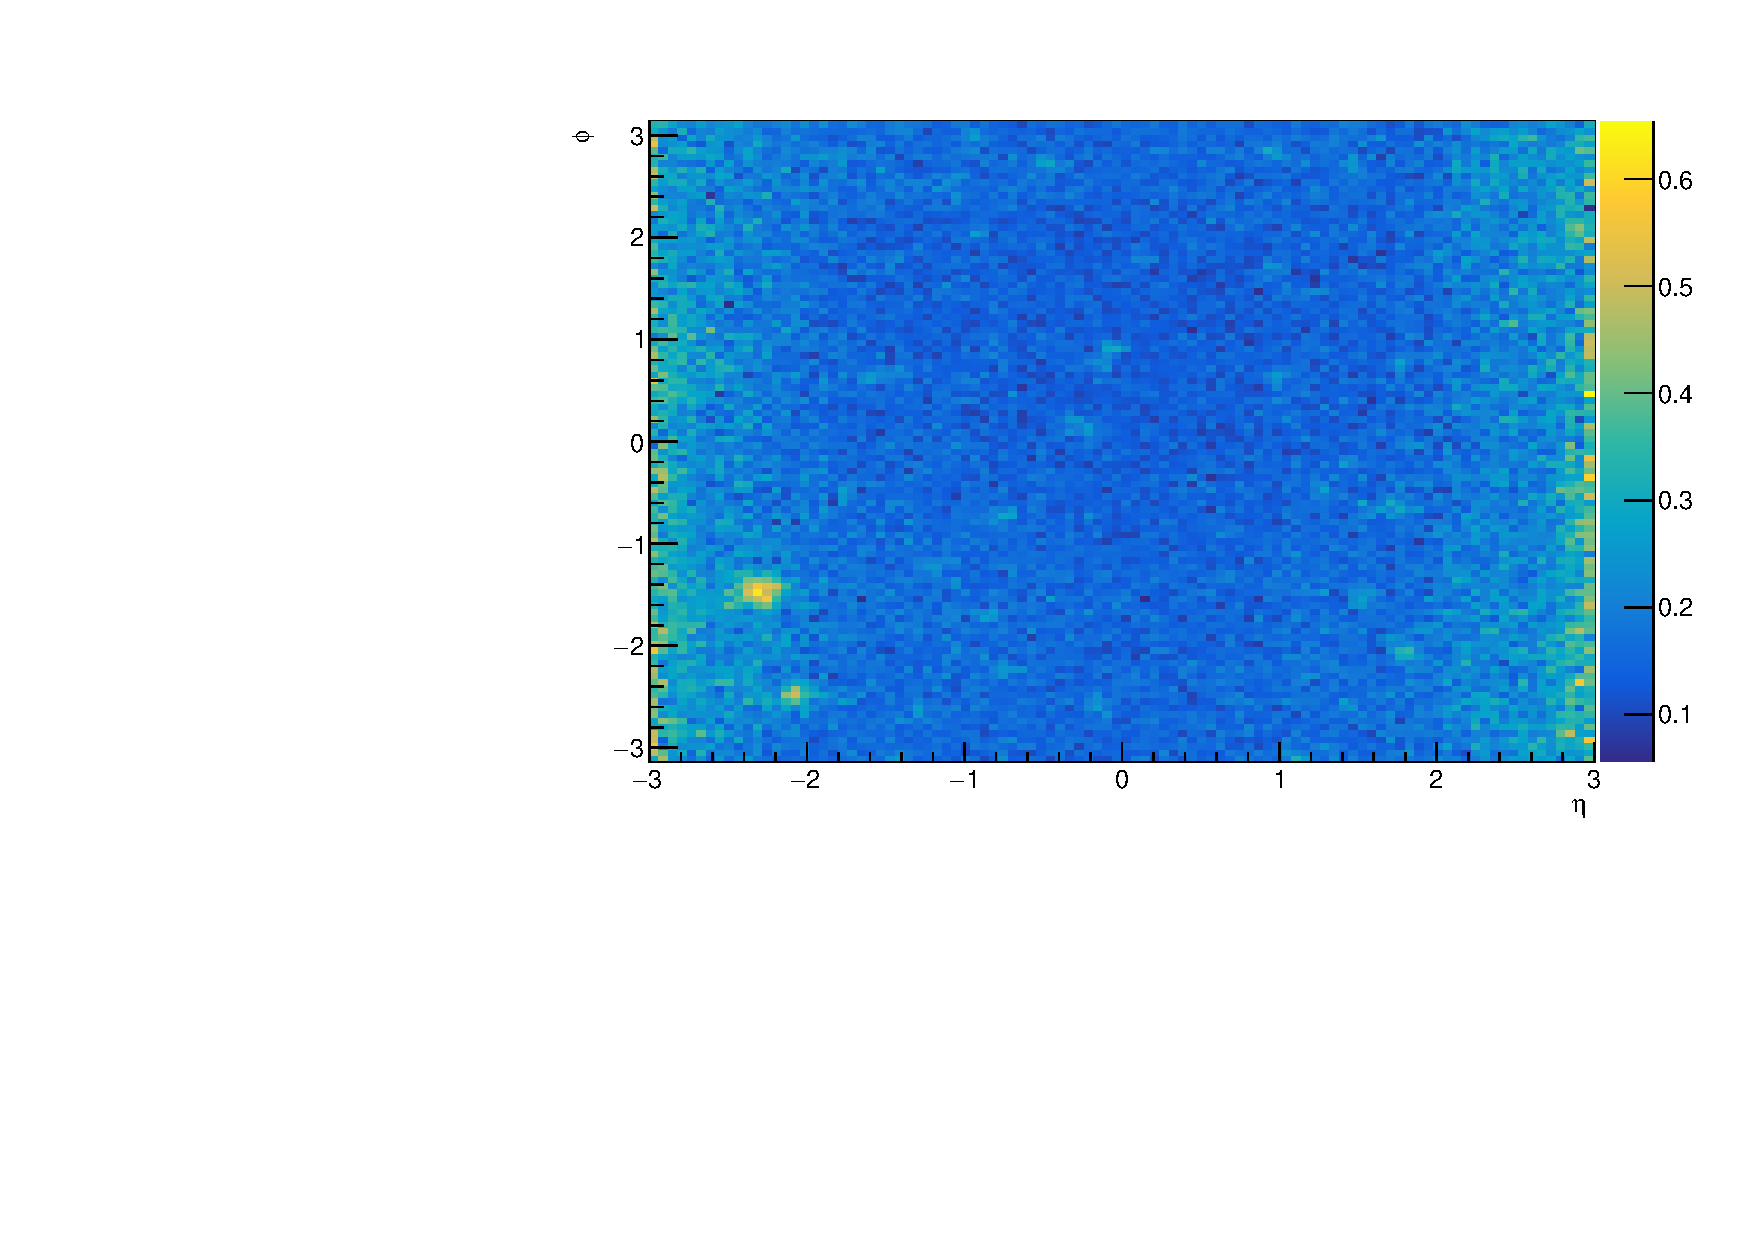
\includegraphics[width=0.7\textwidth]{figures/selection/EtaPhiMap.pdf}}
        \caption{The 2D ratio of jets ($\pt>20\gev$) with $\bdphi<0.3$ plotted in the
        $\eta-\phi$ plane, divided by all jets that satisfy $\pt>20\gev$. 
        Made with 149.49~$\text{pb}^{-1}$ of
        events that pass a loose selection of one good primary vertex,
        $\njet>1$ and $\scalht>150\gev$.}
        \label{fig:2dRatioMap}
    \end{center}
\end{figure}

\begin{figure}[h!]
    \begin{center}
        {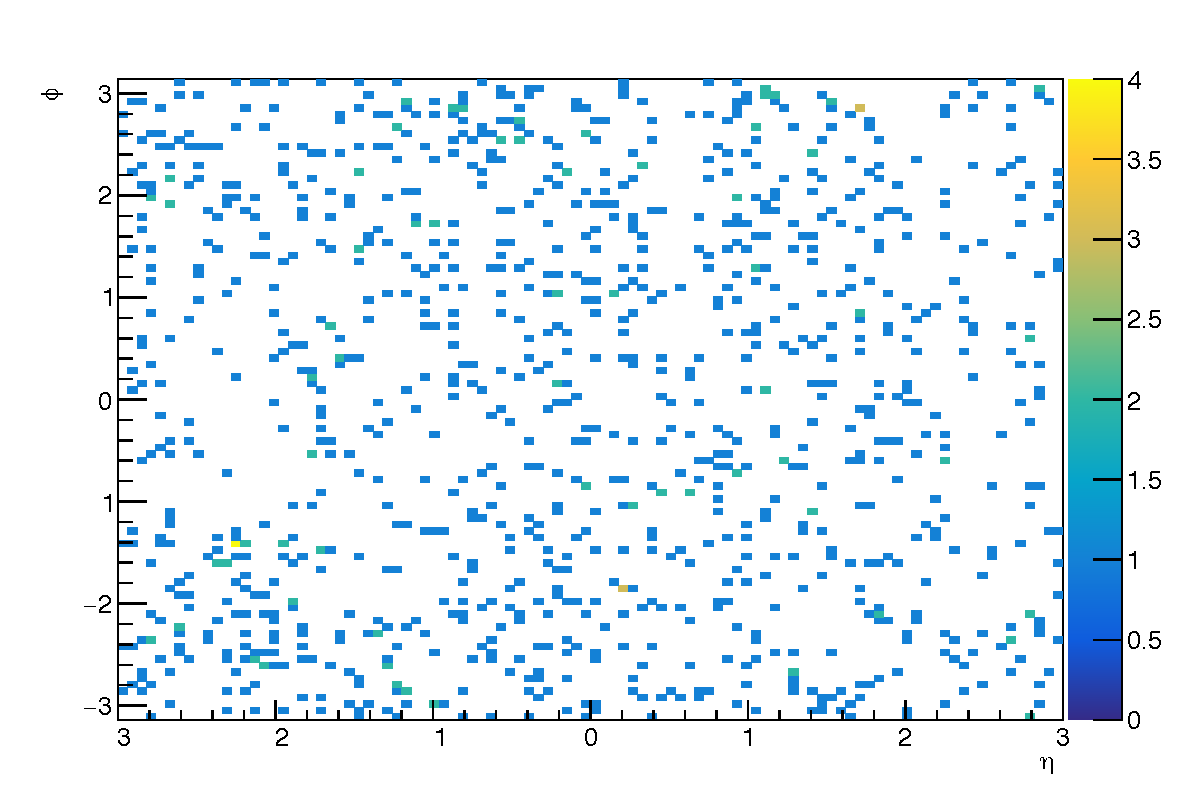
\includegraphics[width=0.7\textwidth]{figures/selection/bDPhilt0p3AfterSelection.pdf}}
        \caption{Jets ($\pt>20\gev$) with $\bdphi<0.3$ plotted in the
        $\eta-\phi$ plane. 
        Made with $1.26\ifb$ of
        events that pass the full signal region selection.}
        \label{fig:jetMapPostSignalSelection}
    \end{center}
\end{figure}

%To protect against severe energy losses caused by masked regions in the ECAL (which
%amount to about 1\% of the ECAL channel count) or HCAL, or by missing
%instrumentation in the barrel-endcap gap, events with $\bdphi < 0.5$
%are rejected if the distance in the ($\eta,\phi$) plane between the
%selected jet and the closest masked ECAL region, $\Delta R_{\rm
%  ECAL}$, is smaller than 0.3. Similarly, events are rejected if the
%jet points within 0.3 in $\eta$ of the ECAL barrel-endcap gap at
%$|\eta| = 1.5$.

{\bf Beam halo.}

The CSC beam halo filter has been found to be less efficient during the early
Run 2 data-taking period compared to the previous run.

Beam halo events manifest themselves as single energy deposits in the
calorimeters, which introduces large amounts of ``fake'' \met. This effect is
especially prominent in the signal region monojet category, particularly at
$\phi$ coordinates of 0 and $\pi$ because of the tendency of halo particles to
lie within the plane of the LHC ring. This is evident in
Fig.~\ref{fig:leadJetCleaning}.

Such spurious events are suppressed by requiring at least 10\% of the leading
jet's energy to originate from charged hadrons, $CHF>0.1$. The effectiveness of this selection
is demonstrated in Fig.~\ref{fig:leadJetCleaning}.

Beyond the filter available in the data ntuples, the JetMET POG have
provided lists of events that should fail the CSC beam halo and bad
ECAL super cluster filters. These extra events are vetoed and the
efficiency of events in the signal region (Sec.~\ref{sec:had-signal})
and single muon control region (Sec.~\ref{subsec:mucontrolSelection})
that pass this veto for each analysis bin are plotted in
Fig.~\ref{fig:cscFilterEfficiencies}. In the vast majority of bins the
extra filters are $100\%$ efficient, with a few bins with an
inefficiency at the $2-3\%$ level. This confirms that the $CHF$ cut is
already effectively removing spurious events that are present due to
beam halo effects. 

\begin{figure}[h!]
    \begin{center}
        {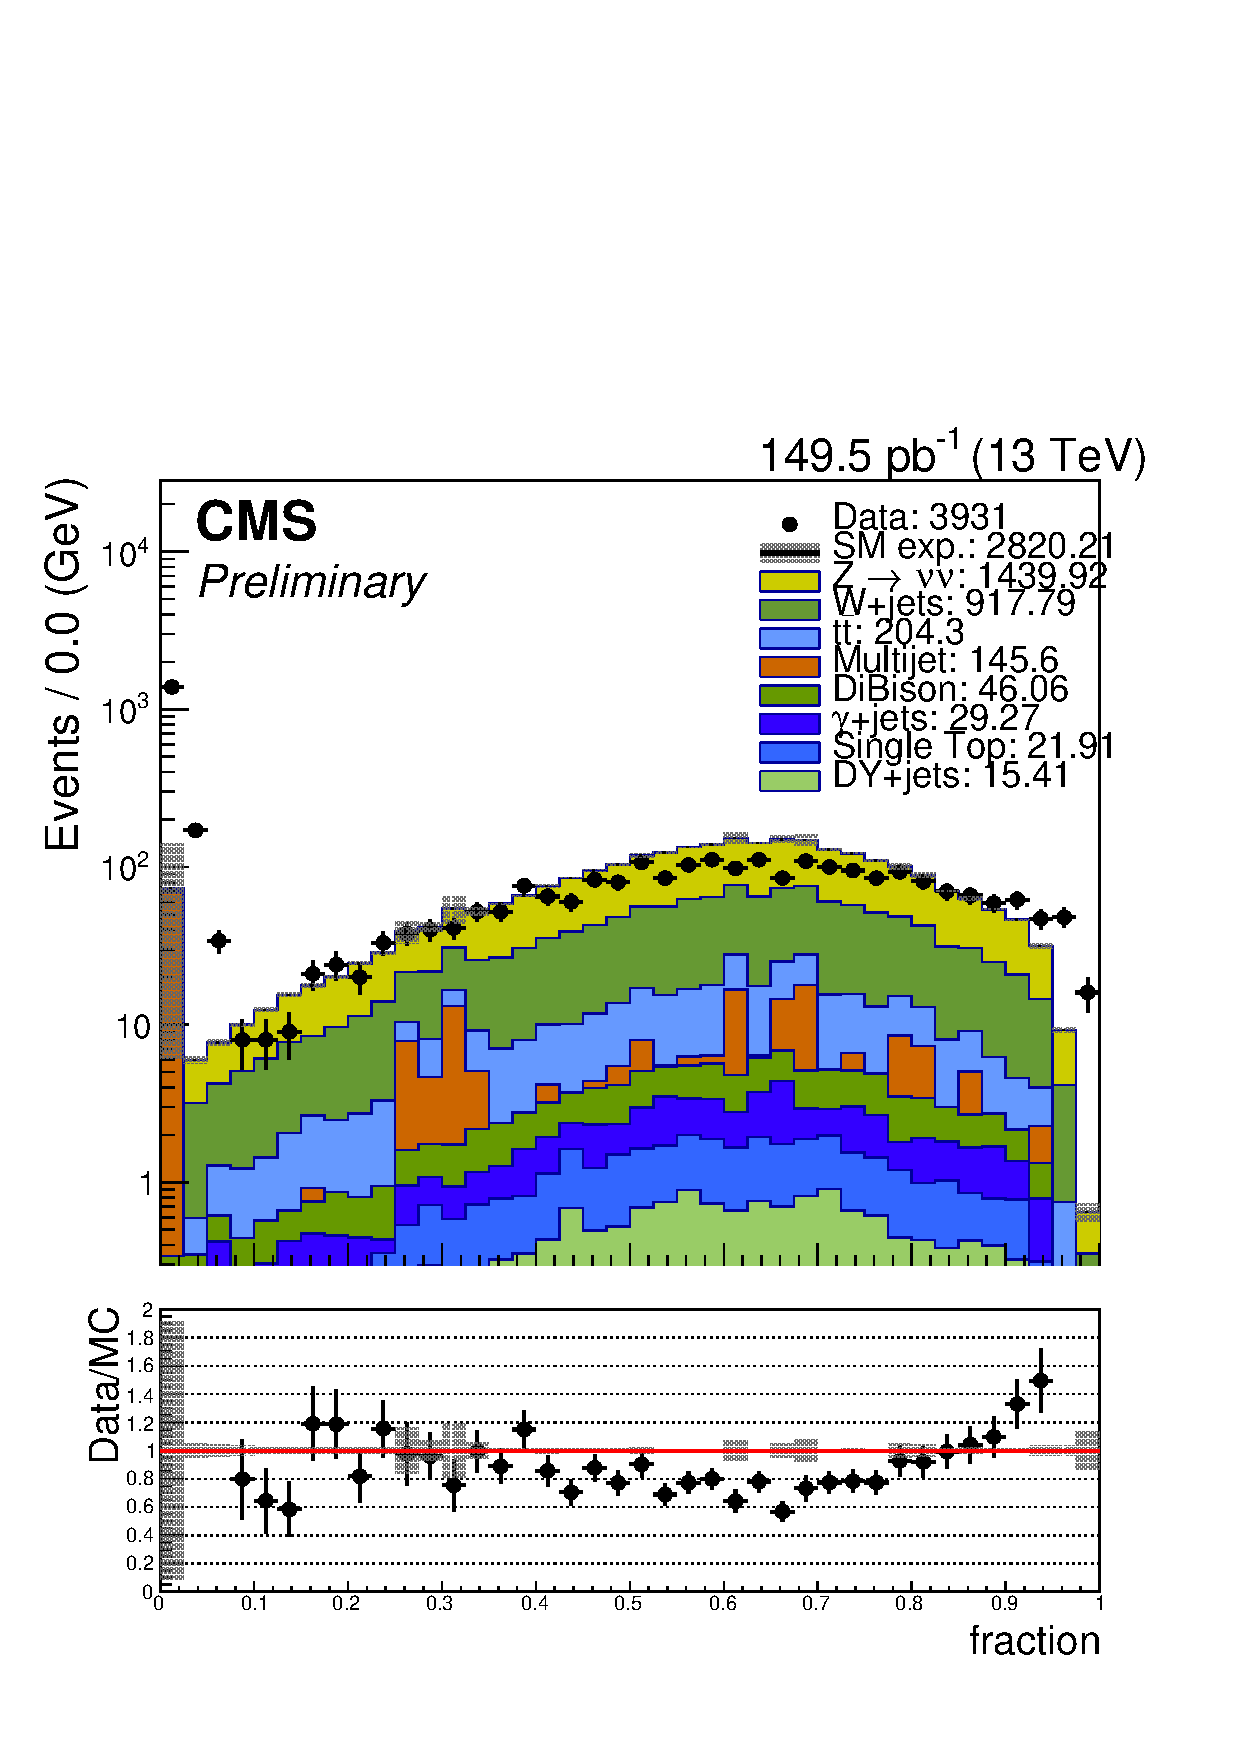
\includegraphics[width=0.32\textwidth]{figures/selection/leadJetChf_all_before.pdf}}
        {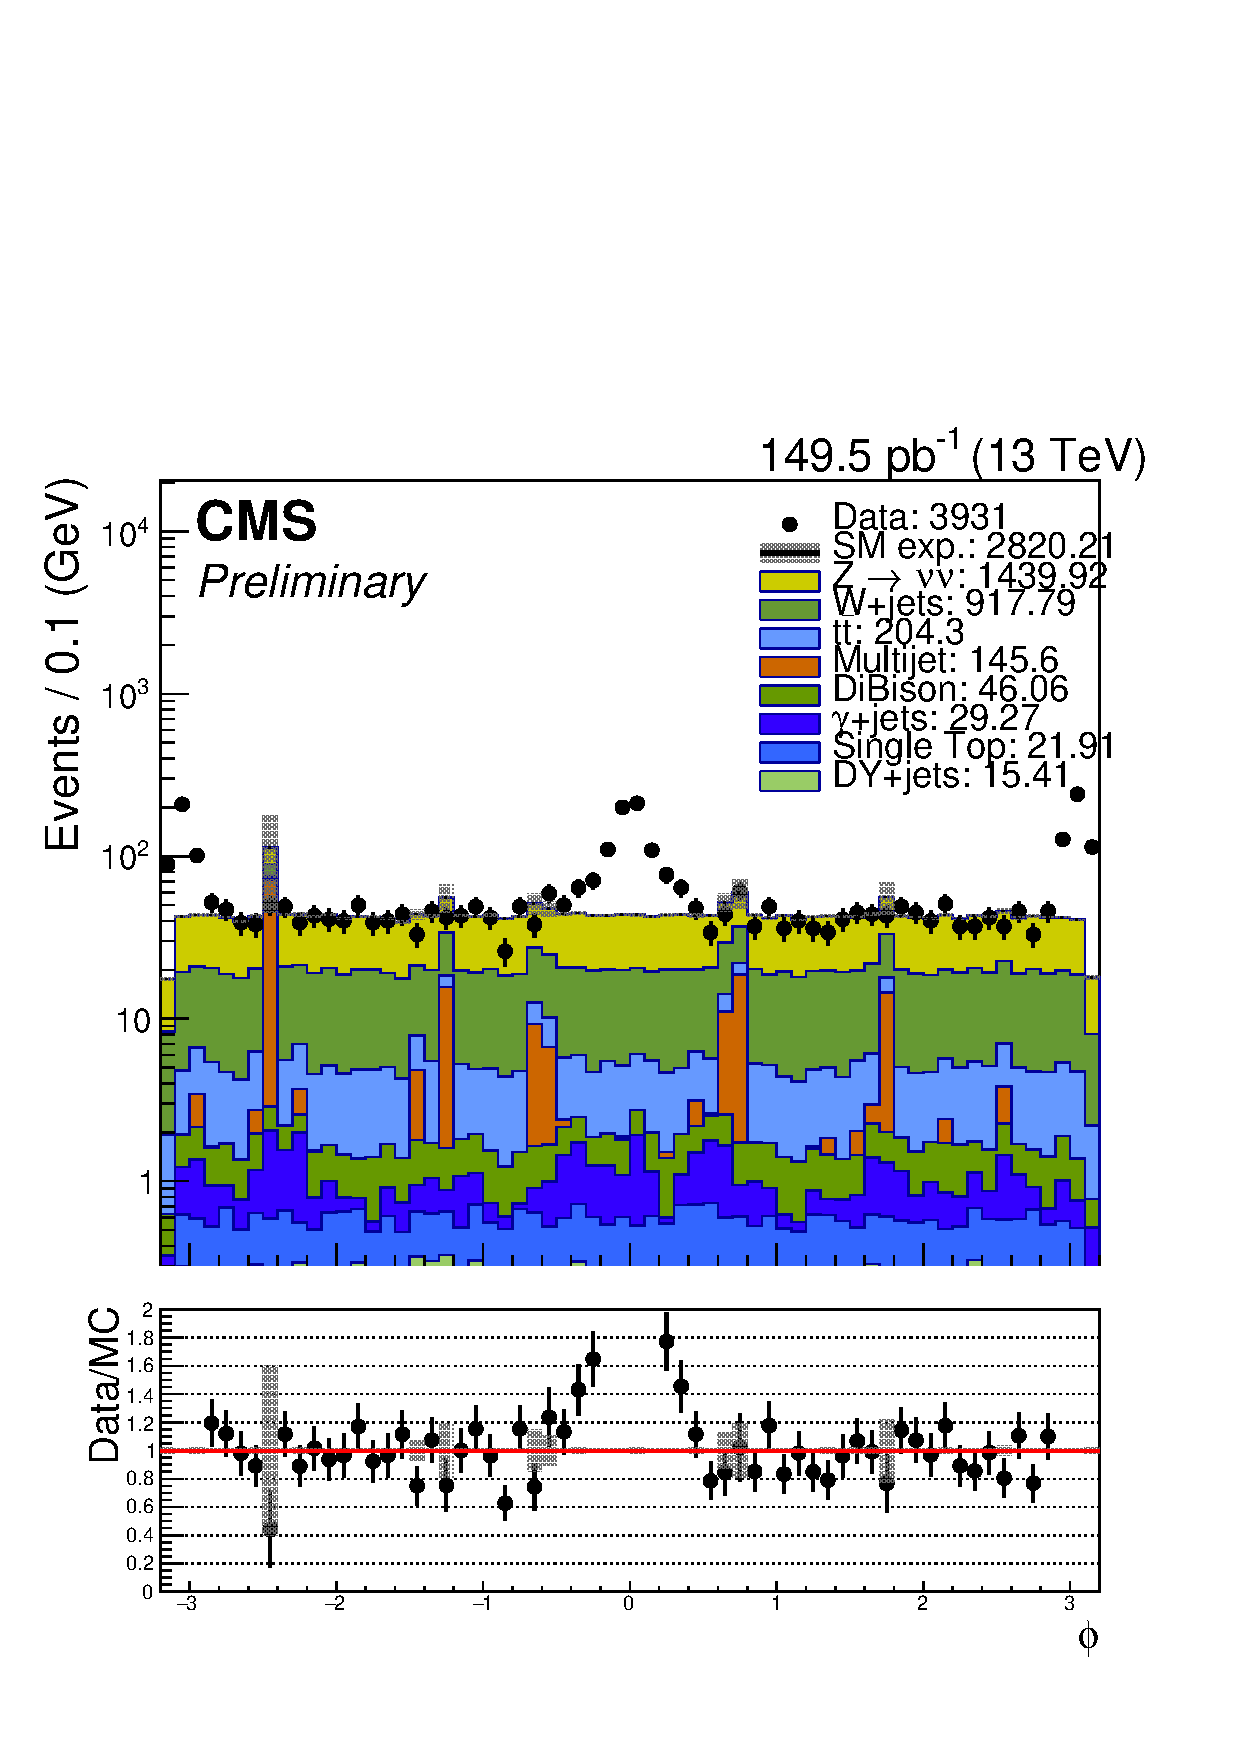
\includegraphics[width=0.32\textwidth]{figures/selection/leadJetPhi_all_before.pdf}}
        {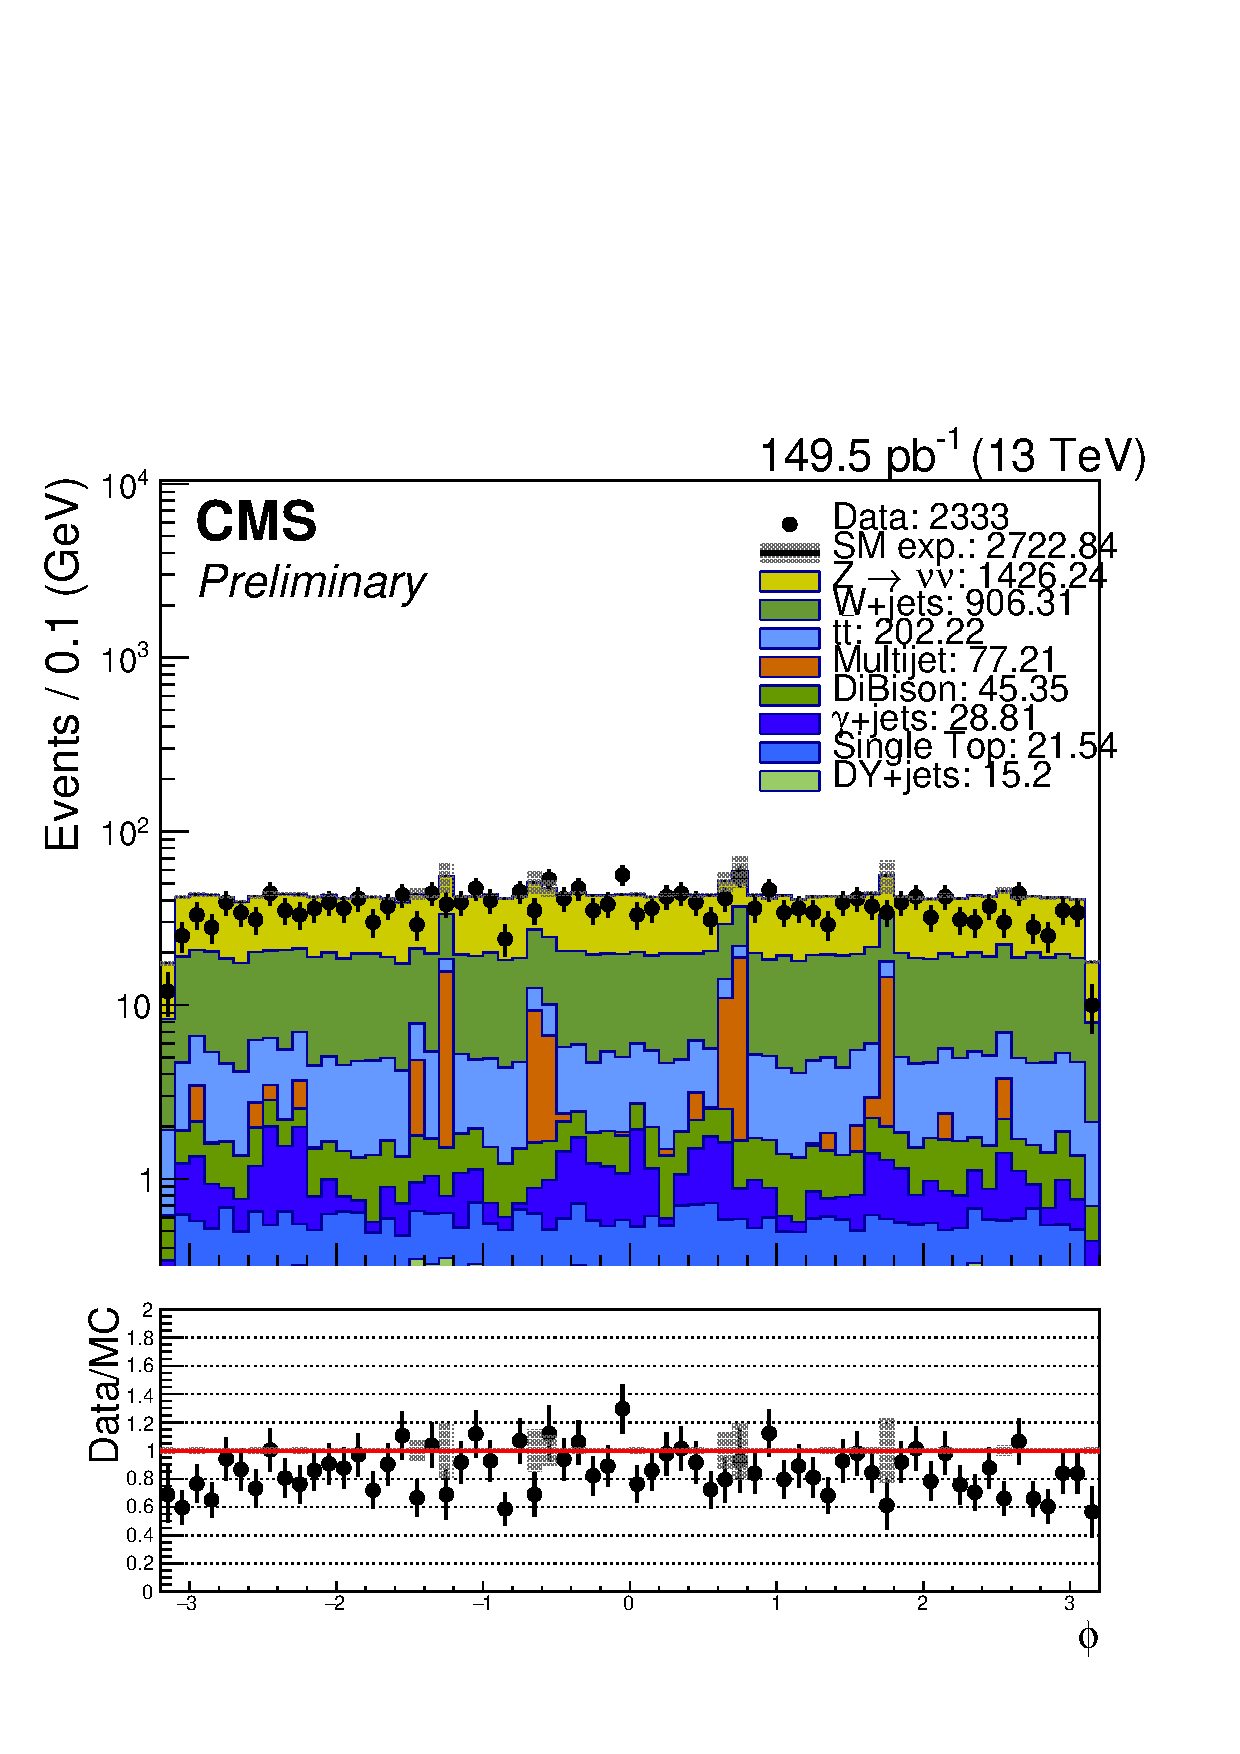
\includegraphics[width=0.32\textwidth]{figures/selection/leadJetPhi_all_after.pdf}}
        \caption{Distributions in the signal region of the lead jet charged hadron
        energy fraction (CHF) (Left), lead jet $\phi$ direction (Centre), and lead jet $\phi$
        direction after applying a requirement of {CHF~$>0.1$}. The large excess in data
        at charged hadron fractions close to zero and ${\phi = 0, \pi}$ is consistent with beam
        halo effects, and is effectively suppressed by the aforementioned selection.}
        \label{fig:leadJetCleaning}
    \end{center}
\end{figure}

\begin{figure}[h!]
  \begin{center}
    \subfigure[Signal region
    selection]{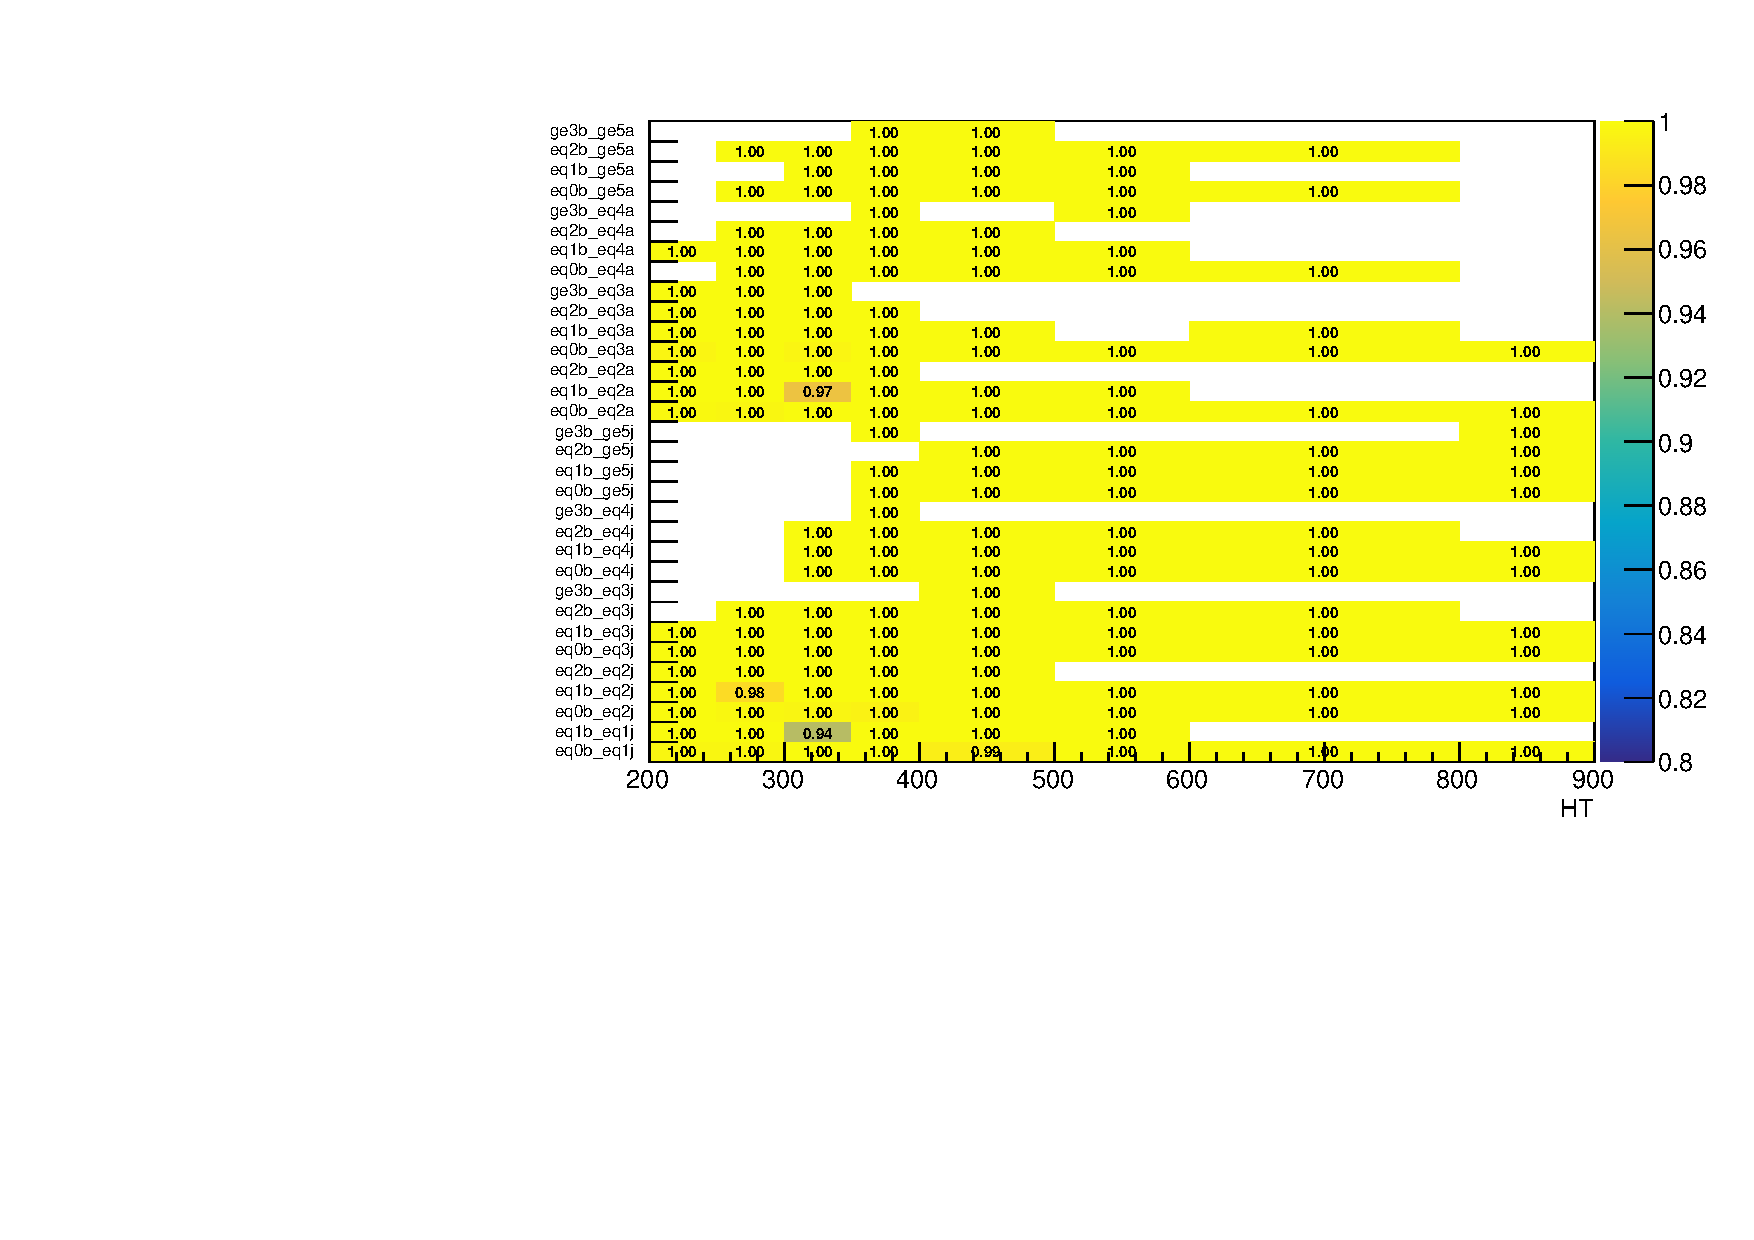
\includegraphics[width=0.5\textwidth]{figures/selection/Signal_Data_CSCEfficiency.pdf}} ~~
    \subfigure[Single muon control region
    selection]{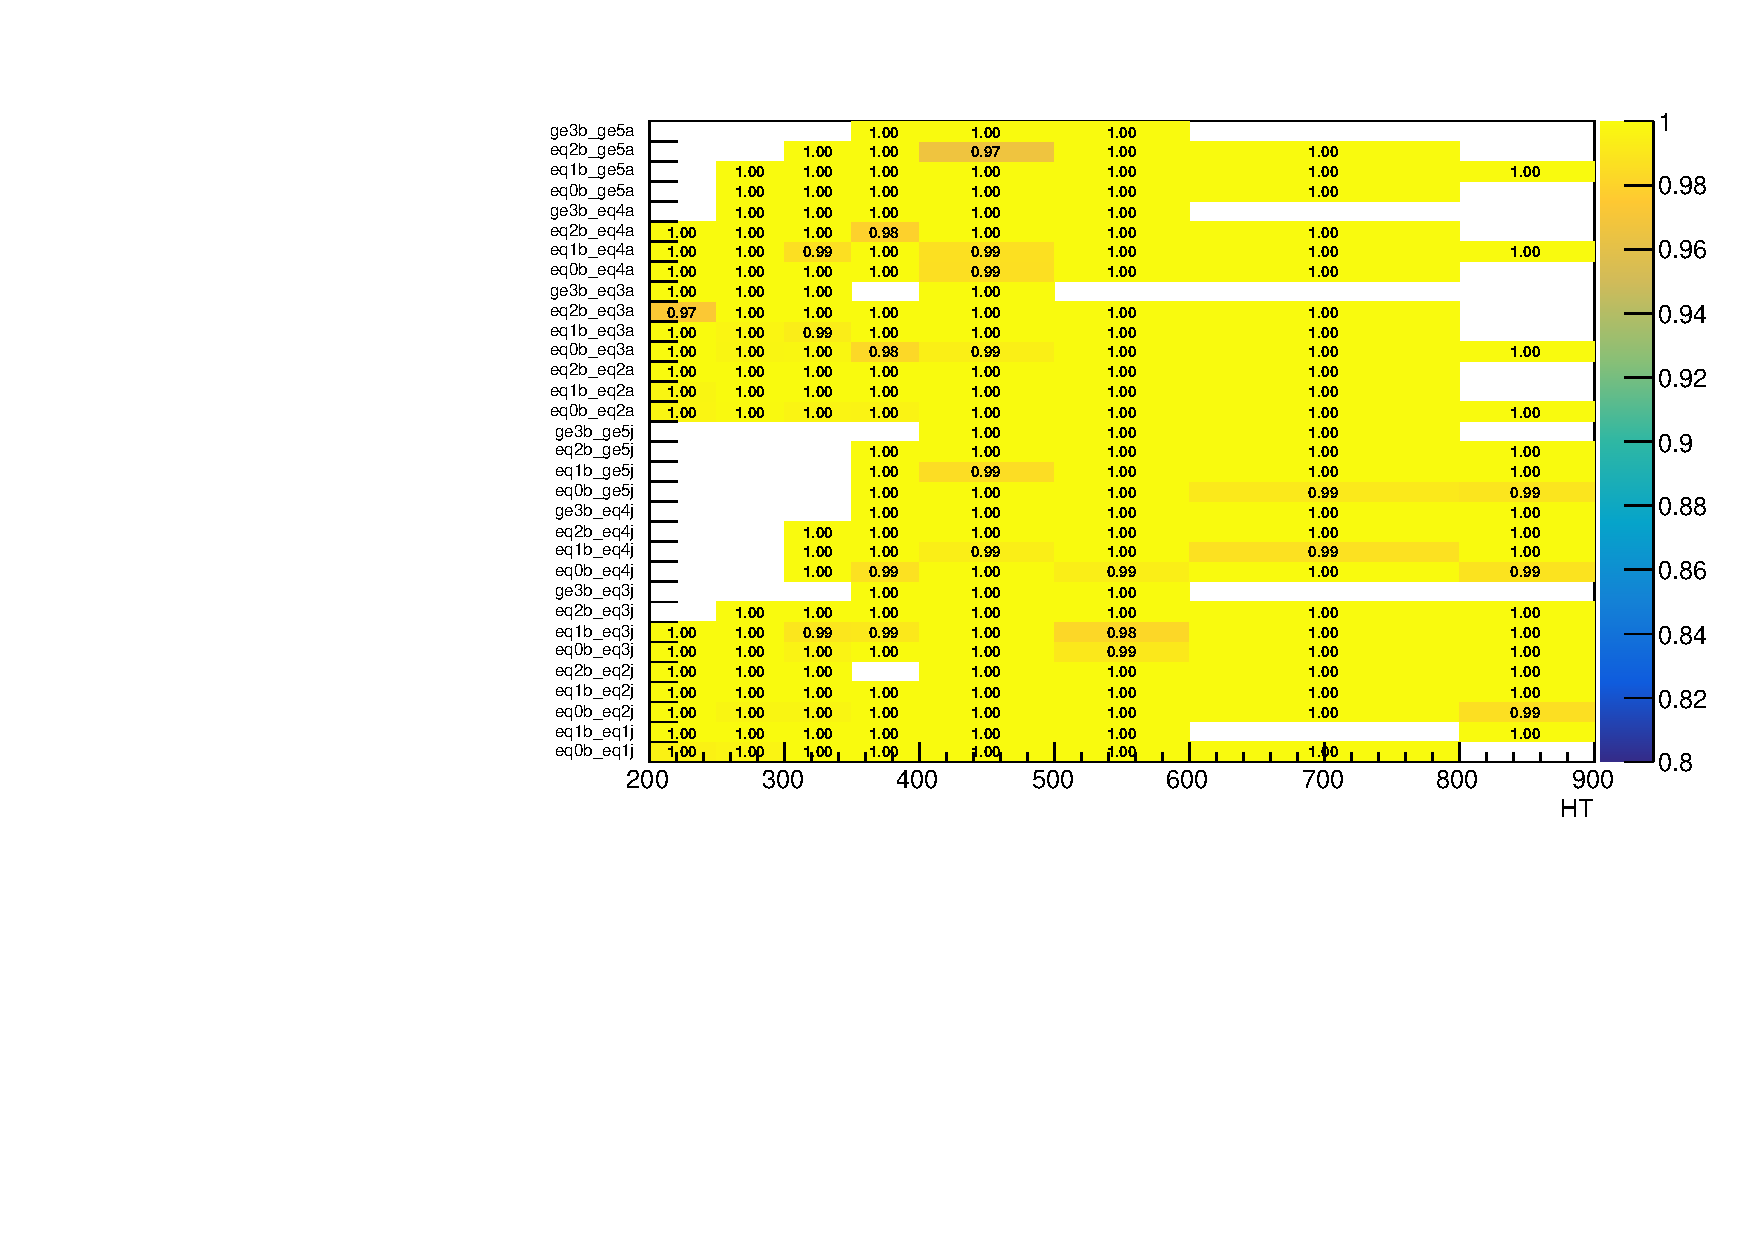
\includegraphics[width=0.5\textwidth]{figures/selection/SingleMu_Data_CSCEfficiency.pdf}} \\
    \caption{Efficiencies of the CSC beam halo and bad ECAL super
    cluster filters applied on $1.26\ifb$ of data passing the single
    muon and signal region selections.}
    \label{fig:cscFilterEfficiencies}
  \end{center} 
\end{figure}

{\bf Summary of signal region selection.} 

The requirements that define the hadronic signal region are summarised
in Table~\ref{tab:sr-selections}.

\begin{table}[h!]
  \topcaption{Summary of the signal region selection criteria, applied
    in addition to the pre-selection summarised in
    Table~\ref{tab:pre-selections}.}
  \label{tab:sr-selections}
  \centering
  \footnotesize
  \begin{tabular}{ ll }
    \hline
    \hline
    Selection             & Requirement                                                    \\
    \hline
    \alphat               & $>$0.52--0.65 (\HT-dependent) for region $200 < \HT < 800\gev$ \\
    \bdphi                & $>0.5$                                                         \\
    \mht/\met             & $<1.25$                                                        \\
    ``Dead ECAL filter''  & (see text)                                                     \\
    ``Beam Halo Filter''  &  $CHF(\textrm{leading jet})>0.1$                                \\

    \hline
    \hline
  \end{tabular}
\end{table}

\subsection{Adding the \texorpdfstring{\mht}{MHT} dimension}
\label{sec:had-shape}

As described above, and as used in Run~1, the analysis takes advantage
of three discriminating variables, \njet, \nb, and \HT, to provide
sensitivity to a large range of SUSY (and DM) models. No extrapolation
in these variables is performed, with predictions of SM background
yields in the (\njet,\nb,\HT) bins of the signal region based on both
observed counts and transfer factors derived from simulated yields in
the corresponding (\njet,\nb,\HT) bins of the control samples. Each
prediction is statistically and systematically independent.

In Run~1, for each (\njet,\nb,\HT) bin in the signal region, an
extrapolation in the variable \alphat was necessary to obtain
background predictions based on the muon control samples, which did
not impose any \alphat requirement. No extrapolation in \alphat was
performed for the photon control sample, which used the same \alphat
requirements as the signal region. The \alphat requirements used in
Run~1 for the signal region correspond loosely to \mht thresholds in
the range $\sim$130 to $\sim$500\gev depending on the \HT
bin. Uncertainties in this extrapolation were determined through
closure tests with respect to data, including one dedicated to the
\alphat extrapolation, plus additional cross checks.

In Run~2, we additionally bin event counts in the signal region
according to the variable \mht in order to provide further
discriminating power between any potential signal and the SM
background counts. Hence, while no extrapolation is performed in
\njet, \nb, nor \HT, the analysis relies on information obtained
from simulation to extrapolate from counts (integrated over \mht) in
the control samples to a predicted distribution in \mht for each
corresponding (\njet,\nb,\HT) bin in the signal region.

The \mht dimension is included in the likelihood model by using
templates determined per (\njet,\nb,\HT) bin from simulation. The
templates use an \mht bin width of 50\gev. The threshold of the final
\mht bin used by the templates is determined based on the size of the
available simulated samples: a statistical uncertainty of not more
than 50\% for the sum of all SM background processes is required. An
associated normalisation nuisance is determined from closure tests
between simulation and data, as described in
Sec.~\ref{sec:syst-on-shape}. Alternative templates are used to encode
the systematic uncertainty in the \mht distribution obtained from
simulation.

\subsection{The hadronic control region}

A hadronic control region that is enriched in multijet events and
disjoint with respect to the signal region is obtained by applying
both the pre-selection criteria and lepton/photon vetoes, as defined
above, and inverting the (\HT-dependent) \alphat and/or \mhtmet
requirements. 
%None of the cleaning filters are not applied to allow the study of
%instrumental effects. 
The sample of events populating this control region are used primarily
to estimate any residual background contamination from QCD multijet
events, described in Sec.~\ref{sec:qcd}.

\subsection{Commonalities between the data control regions}

There are five control regions with leptons or photons in the final
state: \mj, \mmj, and \gj. 
%\ej, \eej, and \gj. 
The full pre-selection is applied as part of the definition of each of these control
regions. The cuts on event-level jet-based quantities are identical to
those applied in the hadronic search region and the same \njet, \nb,
and \scalht binning is used. The lepton(s) or photon is not considered
in the calculation of the event-level variables.

The selection criteria of the various control regions are defined such
that the background composition and event kinematics of the control
regions mirror as closely as possible those for the signal
region. This is done in order to minimise the reliance on the
simulation to model correctly the backgrounds and event kinematics in
the control and signal samples.

Two exceptions are made. First, no \bdphi requirement is imposed as
part of the selection criteria defining the control regions. Second,
in the case of the four leptonic control regions, no requirement is
made on \alphat. This is made possible by the remaining kinematic
selection criteria, which are sufficiently selective to ensure that
the leptonic event samples remain rich in events from the \wj, \ttbar
and \zll processes with negligible contamination from QCD multijet
events. Thus, the acceptance of the leptonic control regions can be
significantly increased, which simultaneously improves their
predictive power and further reduces the effect of any potential
signal contamination.

The lepton event samples can be used to predict components of the SM
background across all \scalht bins, while the \gj sample can only be
used for the region $\HT > 400\gev$ due to the photon trigger
requirements.

\subsection{The \texorpdfstring{\mj}{muon plus jets} control sample}
\label{subsec:mucontrolSelection}

%Events from the \wj and \ttbar processes are found in the hadronic
%signal sample due to unidentified leptons (either out of acceptance or
%not reconstructed) and hadronic tau decays originating from
%high-p$_{T}$ W bosons. An estimate of these background processes is
%obtained through the use of a \mj sample. 

The selection criteria for the \mj sample are chosen to identify W
bosons decaying to a muon and a neutrino in the phase-space of the
signal. In order to select events containing W bosons, exactly one
tight isolated muon within an acceptance of \PT $>$ 30 \gev and
$|\eta| <$ 2.1 is required (due to the trigger), and the transverse
mass of the W candidate must satisfy $30 < \mt(\mu,\pfmet) < 125\gev$
(to suppress QCD multijet and potential signal events). Events are
vetoed if $\Delta R(\mu,\textrm{jet}_i) < 0.5$ running over all jets
$i$. The single isolated track veto, described in
Sections~\ref{sec:objects} and~\ref{sec:vetoes}, is also applied,
which considers all single isolated tracks in the event except that
associated with the identified, isolated muon. Finally, the cleaning
cut $\mht/\met$ is also applied, as done in the signal region, where
the \met is adjusted to account for the transverse momentum of the
identified, isolated muon.

\subsection{The \texorpdfstring{\mmj}{di-muon plus jets} control sample}
\label{subsec:mumucontrolSelection}

%The \znunu\ + jets process forms an irreducible background and can be
%estimated using the \zmumu + jets process, which has similar kinematic
%properties but a different acceptance and a smaller branching ratio. A
%background estimate is obtained through the use of a \mmj sample. 

The selection criteria are identical to those for the \mj sample, with
the following exceptions that are tuned to identify Z bosons decaying
to two muons in the kinematic phase space of the signal region. 
In order to select an event sample containing Z bosons, exactly two
tight isolated muons within an acceptance of $\Pt > 30\gev$ and
$|\eta| < 2.1$ are required (due to the trigger). The invariant mass
of the two muons must satisfy $m_{Z} - 25 < M_{\mu_1\mu_2} < m_{Z} +
25$ and they must have opposite charge. Events are vetoed if $\Delta
R(\mu_{i},\textrm{jet}_j) < 0.5$ is satisfied, running over all muons
$i$ and all jets $j$. The single isolated track veto is also applied
considering all single isolated tracks in the event except those
associated with the two identified, isolated muons. Finally, the
cleaning cut $\mht/\met$ is also applied, as done in the signal
region, where the \met is adjusted to account for the transverse
momenta of the two identified, isolated muons. 

% \subsection{The \texorpdfstring{\ej}{electron plus jets} control sample}
% \label{subsec:elecontrolSelection}
%
% The selection criteria that define the \ej control sample
% mirror those of the \mj sample, \ie, they are tuned
% to identify W boson decaying to an electron and a neutrino in the
% kinematic phase space of the signal region.
%
% Electrons are required to satisfy the Tight working point and satisfy
% the requirements $\Pt> 30\gev$ and $|\eta| < 2.1$. The tightening of
% the Loose working point defined in Sec.~\ref{sec:electron-id} was
% found to greatly reduce multijet contamination without a large
% reduction in statistics within the electron control samples. The
% transverse mass of the W candidate must satisfy $30 < \mt(e,\pfmet)
% < 125\gev$.
%
% \subsection{The \texorpdfstring{\eej}{electron plus jets} control sample}
% \label{subsec:dielecontrolSelection}
%
% The selection criteria that define the \eej control sample
% mirror those of the \mmj sample. They are tuned
% to identify Z boson decaying to a pair of electrons in the
% kinematic phase space of the signal region.
%
% Both electrons need to satisfy Tight working point and the
% requirements $\Pt> 30\gev$ and $|\eta| < 2.1$. The invariant mass of
% the two electrons must satisfy $m_{Z} - 25 < M_{e_1e_2} < m_{Z} + 25$
% and they must have opposite charge.

\subsection{The \texorpdfstring{\gj}{photon plus jets} control sample}
\label{subsec:photoncontrolSelection}

%The \znunu\ + jets process can also be estimated using the \gj
%process, which has a larger cross section and kinematic properties
%similar to those of \znunu\ events when the photon is
%ignored~\cite{PAS-SUS-08-002,Bern:2011pa}. 

The \gj sample is defined by requiring exactly one photon satisfying
tight isolation criteria and within an acceptance of $\pt > 200\gev$
(limited by trigger requirements) and $|\eta| < 1.45$. Furthermore,
events are vetoed if $\Delta R(\gamma,\textrm{jet}_i) < 1.0$ is
satisfied, running over all jets $i$. One important difference with
respect to the leptonic control samples is the application of the
\HT-dependent \alphat requirements imposed as part of the signal
region definition. This is done primarily to ensure that the photon
control sample and signal region are subject to identical kinematic
requirements and the photon carries sufficient transverse energy so
that the mass of the Z boson becomes a negligible effect when using
the \gj sample to predict the kinematic distributions of the \znunu
background. The cleaning cut $\mht/\met$ is also applied, as done in
the signal region, where the \met is adjusted to account for the
transverse energy of the identified, isolated photon. As stated above,
the \gj sample can only be used to predict background components in
the region $\HT > 400\gev$ due to trigger requirements.

\section{The ``b-tag formula method''\label{sec:bjets}}

In order to maximise sensitivity to potential new physics signatures
in final states with multiple b-quark jets, a method that improves the
statistical power of the simulation, particularly for high btag bins, is
employed. This method is known as the ``formula'' method. The
resulting improvement in the statistical precision of the simulation
propagates through to the transfer factors used in the analysis.

\subsection{Method}

The distribution of the number of bjets (\nb) is estimated from generator-level information
contained in the simulation. The number of reconstruction-level jets
matched to underlying bottom quarks ($\nb^{\rm gen}$), charm quarks
($n_{\rm c}^{\rm gen}$), and light-flavoured partons ($n_{\rm
  light}^{\rm gen}$) per event, $N(\nb^{\rm gen},n_{\rm c}^{\rm
  gen},n_{\rm light}^{\rm gen})$, is recorded in bins of (\njet
   , \scalht, \mht). 
 The matching between truth-level partons
and reconstruction-level jets is achieved with a matching algorithm
recommended by the BTV POG~\cite{btagMCTools}.
 The b-tagging efficiency, $\epsilon$, and mistag probabilities,
$f_{\rm c}$ and $f_{\rm light}$, are also determined from simulation
in bins of (\njet,~\scalht,~\mht), with each quantity averaged
over jet $p_{\rm T}$ and $\eta$. Corrections are applied on a
jet-by-jet basis to both $\epsilon$, $f_{\rm c}$, and $f_{\rm light}$
in order to match the corresponding measurements from
data.

The above information is sufficient to predict $\nb$ and thus also
determine the event yield $N(n_{\rm b})$ from simulation for a given
bin in (\njet,~\scalht,~\mht) with the expression:

\begin{equation}
  \label{equ:btag-formula}
  N(n_{\textrm{b}}) = \sum_{n_{\textrm{jet}}} \, \sum_{n_{\textrm{b}}}
  \left( \, N(n_{\textrm{b}}^{\textrm{gen}},
    n_{\textrm{c}}^{\textrm{gen}}, n_{\textrm{l}}^{\textrm{gen}})
    \times P_{\rm b} \times P_{\rm c} \times P_{\rm light} \, \right) \, , 
\end{equation}

with $n_{\textrm{b}}^{\textrm{tag}}$,
$n_{\textrm{c}}^{\textrm{tag}}$, and $n_{\textrm{l}}^{\textrm{tag}}$
defined the number of times that a reconstructed b-quark jet is identified
as originating from an underlying bottom quark, charm quark, or
light-flavoured parton, respectively, and $P_{\rm b} \equiv
P(n_{\textrm{b}}^{\textrm{tag}} ; n_{\textrm{b}}^{\textrm{gen}},
\epsilon)$, $P_{\rm c} \equiv P(n_{\textrm{c}}^{\textrm{tag}} ;
n_{\textrm{c}}^{\textrm{gen}}, f_{\rm c})$, and $P_{\rm light} \equiv
P(n_{\textrm{l}}^{\textrm{tag}} ; n_{\textrm{l}}^{\textrm{gen}},
f_{\rm light})$ as the binomial probabilities for this to happen.
The outer summation considers all possible combinations of
$n_{\textrm{b}}^{\textrm{gen}}$, $n_{\textrm{c}}^{\textrm{gen}}$, and
$n_{\textrm{l}}^{\textrm{gen}}$ that satisfy $n_{\textrm{jet}} =
n_{\textrm{b}}^{\textrm{gen}} + n_{\textrm{c}}^{\textrm{gen}} +
n_{\textrm{l}}^{\textrm{gen}}$ with $n_{\textrm{jet}}$ defined as the number 
of jets in the event, while the inner summation considers
all possible combinations of $n_{\textrm{b}}^{\textrm{tag}}$,
$n_{\textrm{c}}^{\textrm{tag}}$, and $n_{\textrm{l}}^{\textrm{tag}}$
that satisfy $n_{\textrm{b}} = n_{\textrm{b}}^{\textrm{tag}} +
n_{\textrm{c}}^{\textrm{tag}} + n_{\textrm{l}}^{\textrm{tag}}$.
  
The method exploits the ability to make precise measurements of
$N(n_{\rm b}^{\rm gen},n_{\rm c}^{\rm gen},n_{\rm light}^{\rm gen})$,
$\epsilon$, $f_{\rm c}$, and $f_{\rm light}$ independently of $n_{\rm
  b}$, which means that event yields for a given b-quark jet
multiplicity can be predicted with a higher statistical precision than
obtained directly from simulation. Precise measurements of $f_{\rm c}$
and $f_{\rm light}$ are particularly important for events with $n_{\rm
  b} \geq 3$, which often occur in the SM because of the presence of
mistagged jets in the event. In this case, the largest background is
\ttbar, with two correctly tagged b-quark jets and an additional
mistagged jet originating from a charm quark or light-flavoured
parton.

\subsection{Validation}

Predictions from the formula method are used to construct transfer 
factors as described in Section~\ref{sec:backgroundmet} and \mht shape distribution
 as described in Section~\ref{sec:syst-on-shape}. Predictions are made
 with the extrapolation to high \nb bins on MC level only.

Figure~\ref{fig:mhtShape_ge5j_ge3b_ht600} and ~\ref{fig:mhtShape_ge5j_ge3b_ht800} 
compare the \nb~distributions between predictions from formula method and raw MC. Figure~\ref{fig:pull} shows
the pull distribution, where the pull is defined as the prediction from
 formula method and raw MC yields in each (\njet,~\scalht,~\mht) bin divided by statistical
 uncertainties, of predictions from formula method to raw MC. 
This demonstrates closure between formula and raw MC, as expected because 
 all the quantities in equation~\ref{equ:btag-formula} are computed in MC simulations and 
 no data driven corrections, such as btag scale factors from BTV, have been injected at this level.

Table~\ref{tab:formula-ge5j} compares
predictions from formula method to raw MC yields for the jet category \njet $\geq 5$. 
Statistical uncertainties are generally smaller with formula
method, and in some bins formula method allows extrapolation at high btag bins 
where raw MC suffers from low or even no statistic.

 \begin{figure}[h!]
  \centering
  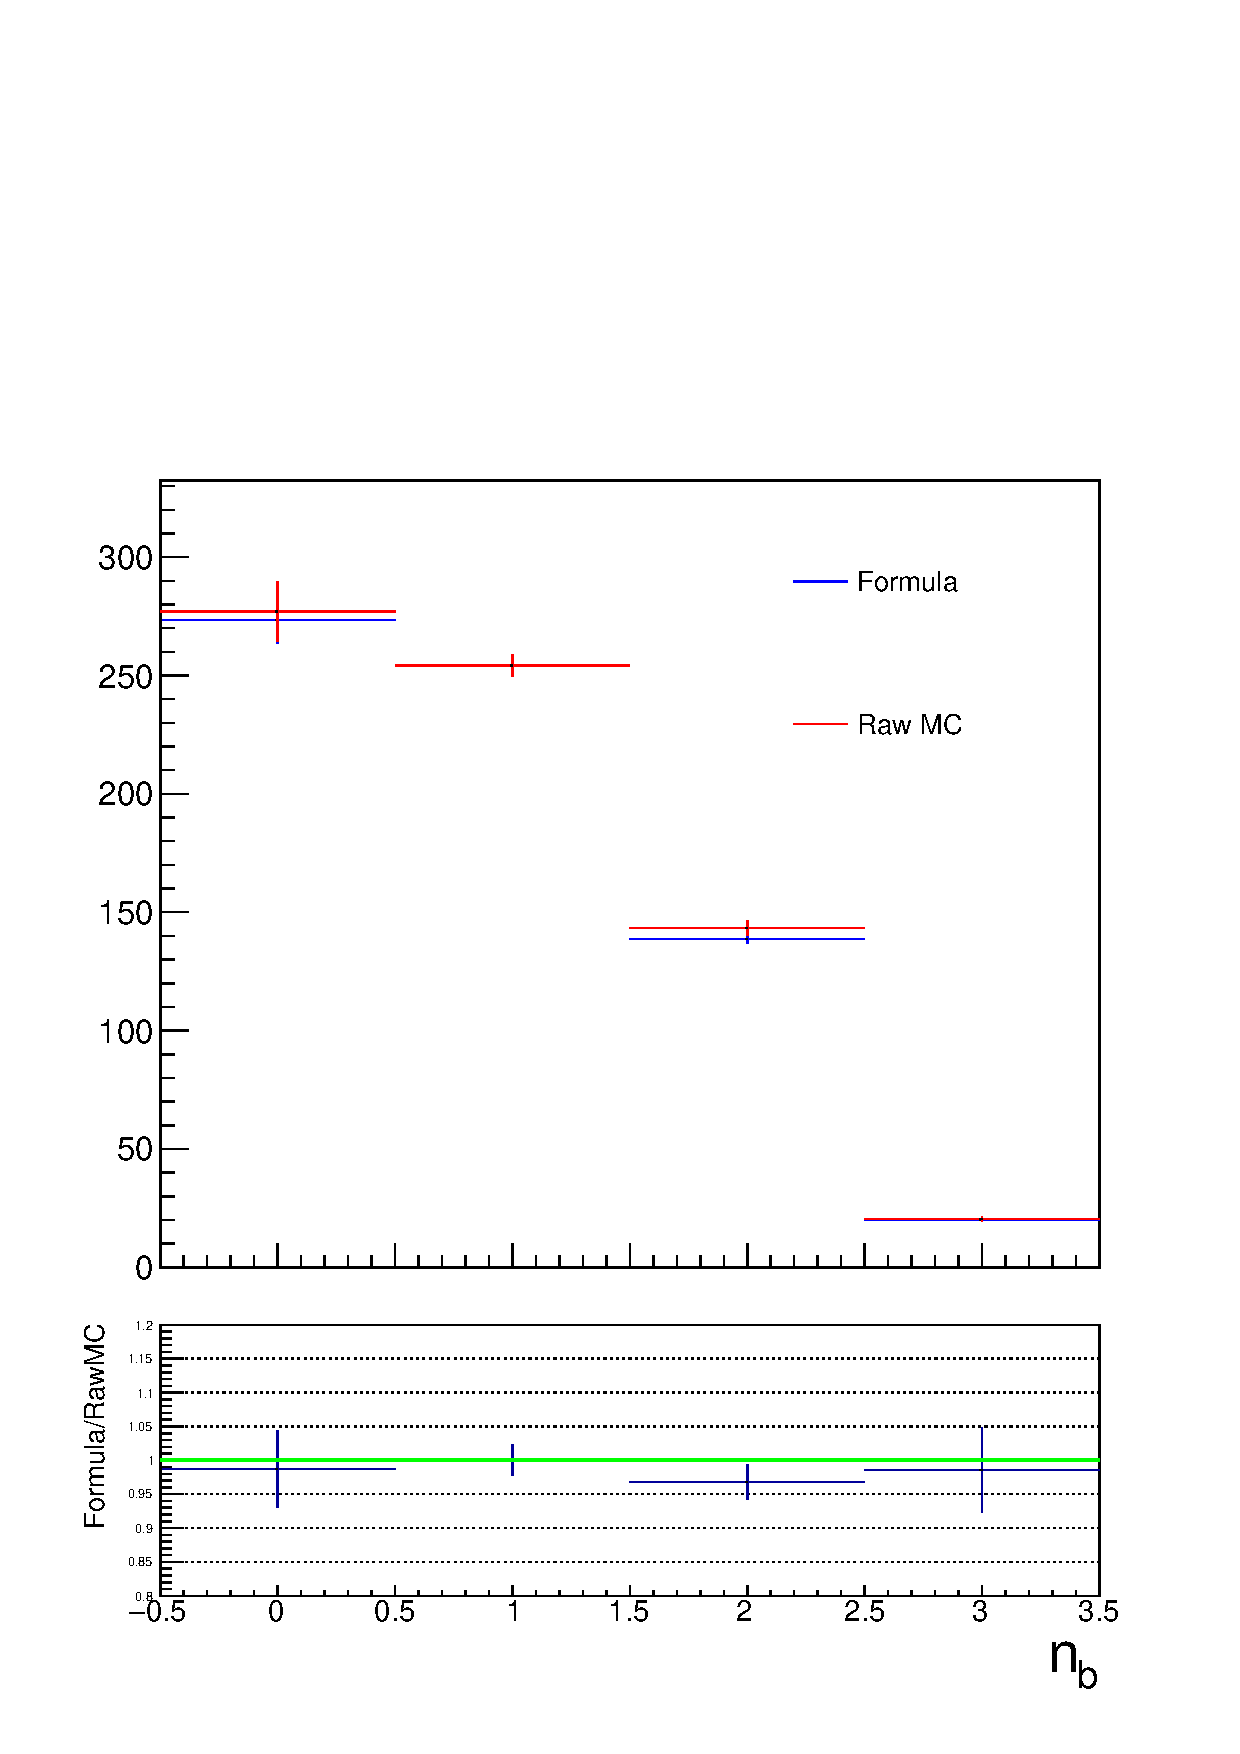
\includegraphics[width=0.7\textwidth]{figures/btagformula/ge5j_600_0_Inc_GoodNb.pdf} 
  \caption{\label{fig:mhtShape_ge5j_ge3b_ht600} \nb distribution from formula
   method (Blue) and raw MC (Red) for the bin \scalht~$600-800$, \njet $\geq 5$, inclusive
   in \mht.}
\end{figure}

 \begin{figure}[h!]
  \centering
  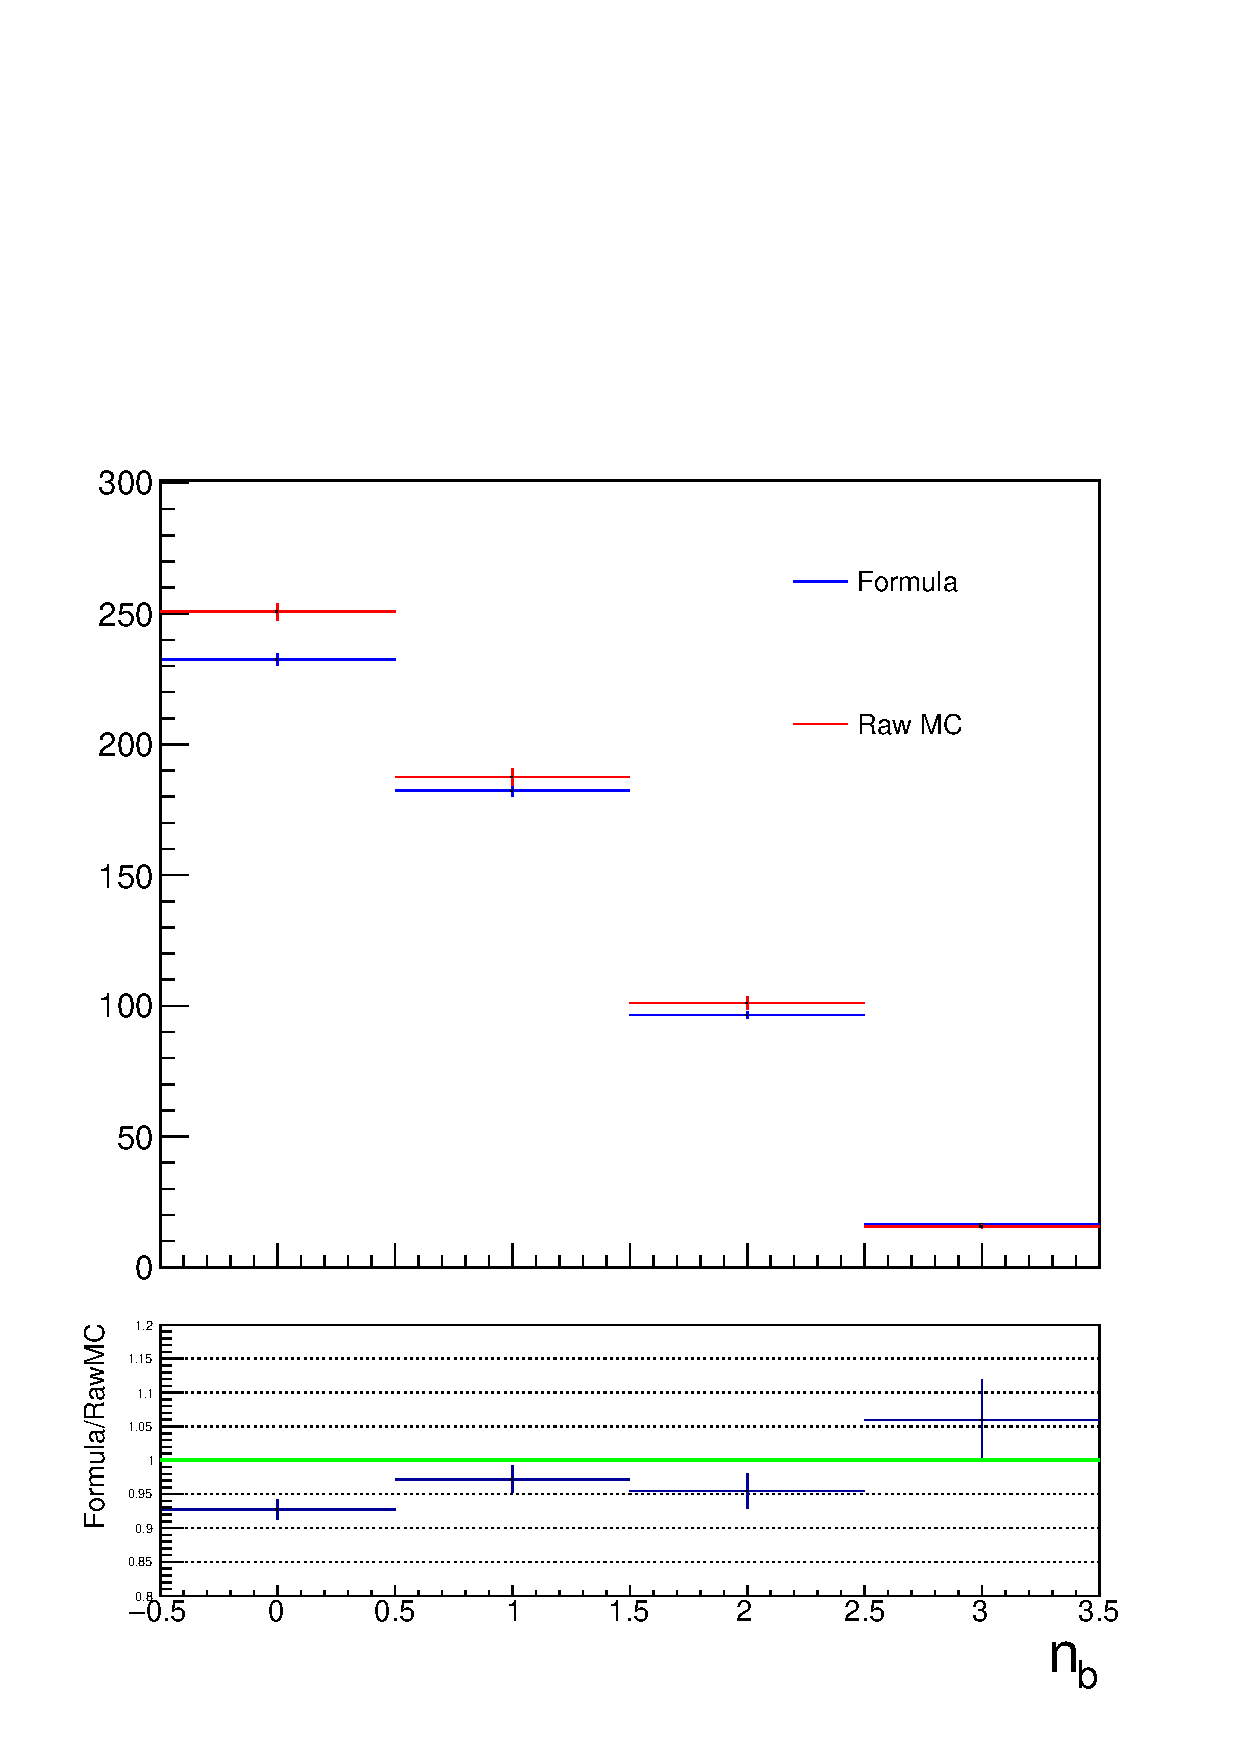
\includegraphics[width=0.7\textwidth]{figures/btagformula/ge5j_800_0_Inc_GoodNb.pdf} 
  \caption{\label{fig:mhtShape_ge5j_ge3b_ht800} \nb~distribution from formula
   method (Blue) and raw MC (Red) for the bin \scalht~$800-\infty$, \njet $\geq 5$, inclusive
   in \mht.}
\end{figure}


 \begin{figure}[h!]
  \centering
  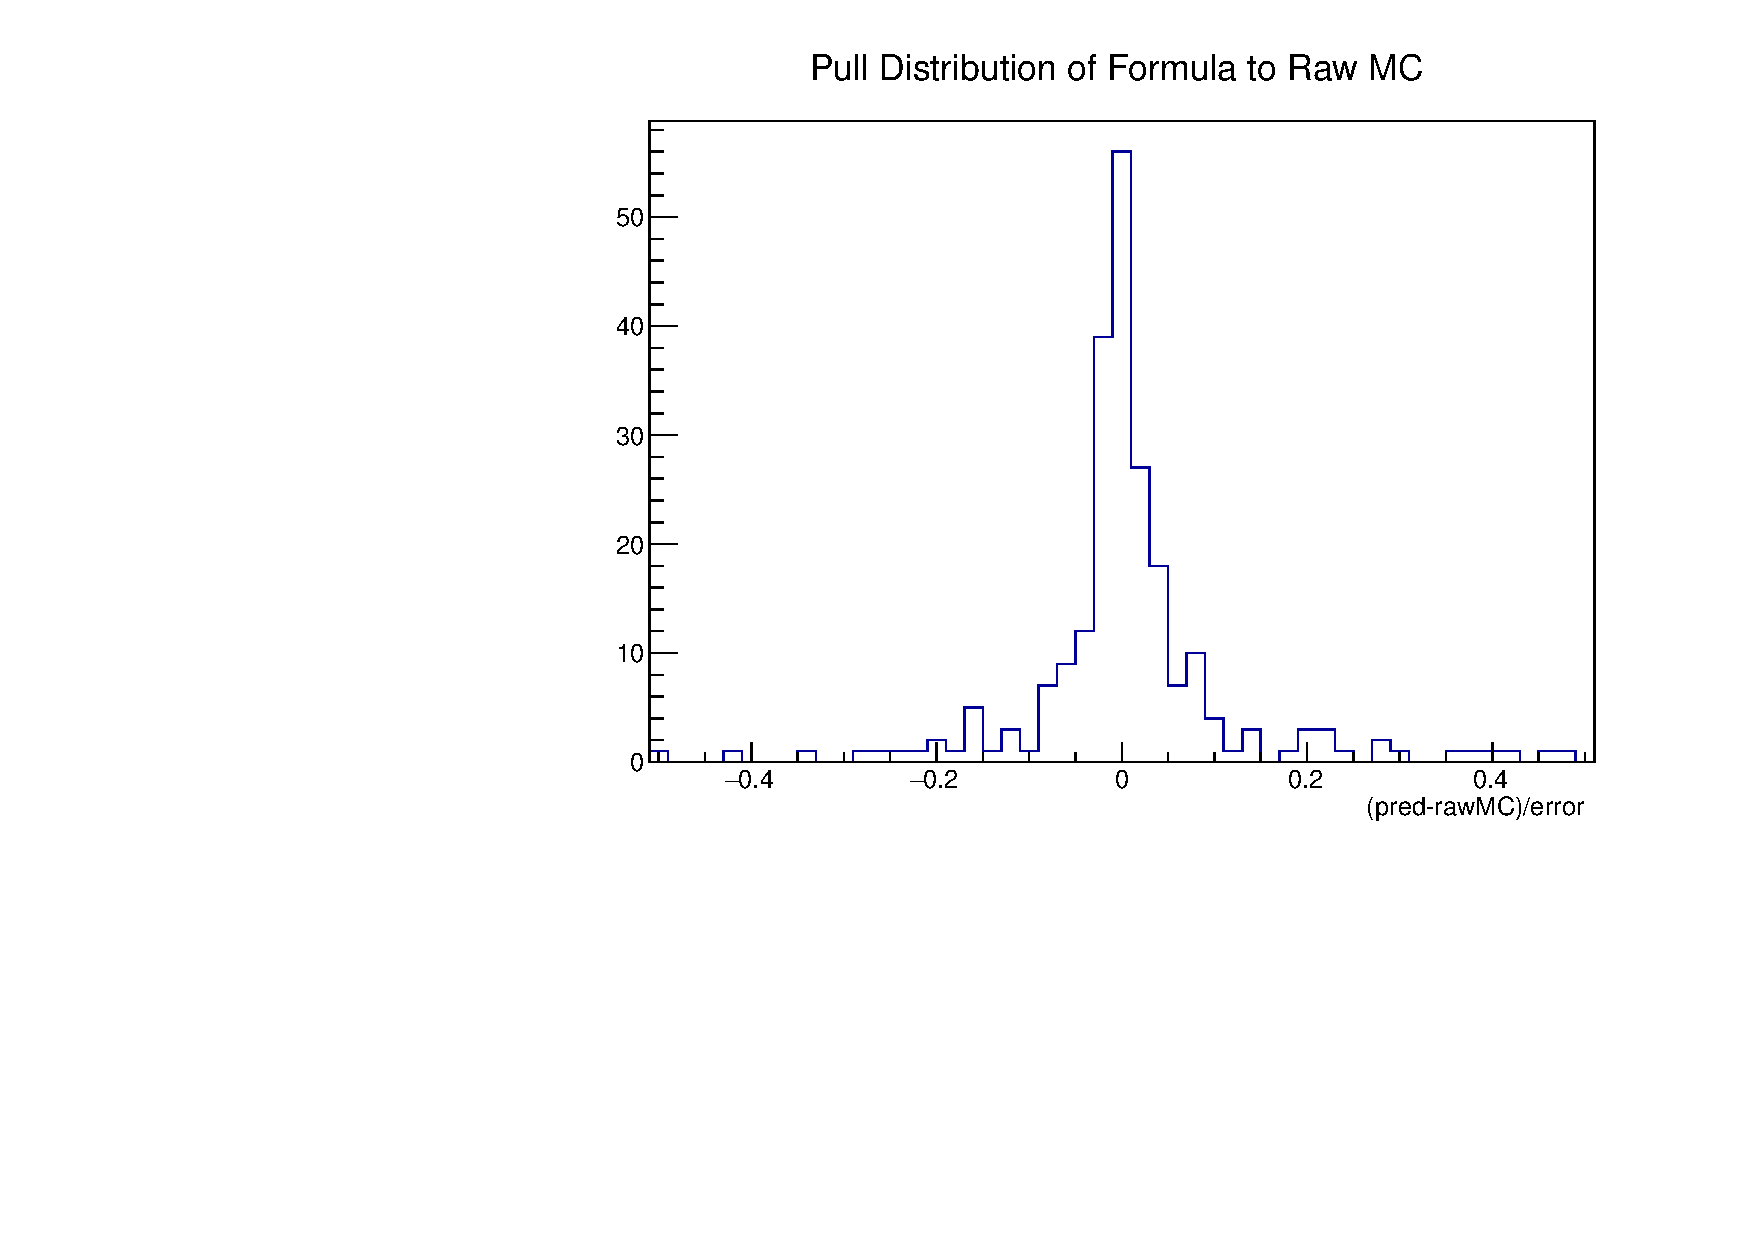
\includegraphics[width=0.8\textwidth]{figures/btagformula/pull.pdf} 
  \caption{\label{fig:pull} Pull Distribution of prediction from formula to raw MC}
\end{figure}

\begin{figure}
\definecolor{Red}{rgb}{1,0,0}
\begin{longtable}{ | c | c | c | c | c | c | c | }
\caption{Comparison between predictions from formula method and raw MC ge5j} \label{tab:formula-ge5j} \\    \hline 
$H_{T}$ & $H_{T}^{miss}$ & Method & $n_{b} = 0$ & $n_{b} = 1$ & $n_{b} = 2$ & $n_{b} \ge 3$ \\ \hline200,250 & 0,Inf & Formula  & $     0.00 \pm  0.00 $ & $     0.00 \pm  0.00 $ & $     0.00 \pm  0.00 $ & $     0.00 \pm  0.00 $  \\  
200,250 & 0,Inf & Vanilla  & $     0.00 \pm  0.00 $ & $     0.00 \pm  0.00 $ & $     0.00 \pm  0.00 $ & $     0.00 \pm  0.00 $  \\ \hline 
250,300 & 0,Inf & Formula  & $     0.00 \pm  0.00 $ & $     0.00 \pm  0.00 $ & $     0.00 \pm  0.00 $ & $     0.00 \pm  0.00 $  \\  
250,300 & 0,Inf & Vanilla  & $     0.00 \pm  0.00 $ & $     0.00 \pm  0.00 $ & $     0.00 \pm  0.00 $ & $     0.00 \pm  0.00 $  \\ \hline 
300,350 & 0,Inf & Formula  & $     0.60 \pm  0.69 $ & $     0.19 \pm  0.32 $ & $     0.05 \pm  0.21 $ & $     0.00 \pm  0.03 $  \\  
300,350 & 0,Inf & Vanilla  & $     0.67 \pm  0.70 $ & $     0.00 \pm  0.06 $ & $     0.17 \pm  0.34 $ & $     0.00 \pm  0.00 $  \\ \hline 
350,400 & 0,Inf & Formula  & $    13.25 \pm  1.30 $ & $    13.65 \pm  0.91 $ & $     6.78 \pm  0.75 $ & $     0.41 \pm  0.30 $  \\  
350,400 & 0,Inf & Vanilla  & $    11.96 \pm  1.32 $ & $    14.79 \pm  1.21 $ & $     6.99 \pm  0.83 $ & $     0.35 \pm  0.35 $  \\ \hline 
400,500 & 0,Inf & Formula  & $   131.16 \pm  2.13 $ & $   141.75 \pm  1.52 $ & $    74.01 \pm  1.28 $ & $     8.00 \pm  0.65 $  \\  
400,500 & 0,Inf & Vanilla  & $   122.24 \pm  2.20 $ & $   141.90 \pm  1.88 $ & $    81.08 \pm  1.59 $ & $     9.70 \pm  0.90 $  \\ \hline 
500,600 & 0,Inf & Formula  & $   182.42 \pm  2.15 $ & $   195.47 \pm  1.64 $ & $   106.09 \pm  1.39 $ & $    13.33 \pm  0.74 $  \\  
500,600 & 0,Inf & Vanilla  & $   170.70 \pm  2.23 $ & $   192.11 \pm  2.03 $ & $   121.03 \pm  1.74 $ & $    14.49 \pm  1.05 $  \\ \hline 
600,800 & 0,Inf & Formula  & $   273.40 \pm  3.12 $ & $   254.30 \pm  1.92 $ & $   138.76 \pm  1.44 $ & $    20.19 \pm  0.77 $  \\  
600,800 & 0,Inf & Vanilla  & $   264.33 \pm  3.54 $ & $   251.09 \pm  2.14 $ & $   155.71 \pm  1.84 $ & $    22.79 \pm  1.13 $  \\ \hline 
800,Inf & 0,Inf & Formula  & $   232.54 \pm  1.54 $ & $   182.29 \pm  1.44 $ & $    96.55 \pm  1.14 $ & $    16.56 \pm  0.56 $  \\  
800,Inf & 0,Inf & Vanilla  & $   243.47 \pm  1.75 $ & $   184.93 \pm  1.80 $ & $   107.57 \pm  1.60 $ & $    16.88 \pm  0.95 $  \\ \hline 
    \hline 
    \hline 
\end{longtable}
\end{figure}

\subsection{Systematic uncertainties on transfer factors\label{sec:btag-syst}}
Predictions from formula method are treated in the same way as raw MC yields, 
and hence subject to all systematic sources in the analysis. For the data driven normalisation 
uncertainties which affect the total number of events in each (\njet,~\nb,~\scalht) bin, 
most of the systematics are derived inclusively in \nb. Formula method only changes
the W/\ttbar admixture closure test in Section~\ref{sec:tfSyst_WttAd}. 
The corresponding result is shown in Figure~\ref{fig:closureBTag-formula}. No significant changes are expected from the same test with raw MC.

The systematic on transfer factors from btag scale factors is tested by varying 
the btag scale factors up and down. The results are shown in
 from Figure~\ref{fig:tfSyst_bsf_muToZinv-formula} to Figure~\ref{fig:tfSyst_bsf_muToTtw-formula}.
They are typically in the range of $1-5\%$.


\begin{figure}[h!]
  \begin{center}
    \subfigure[]{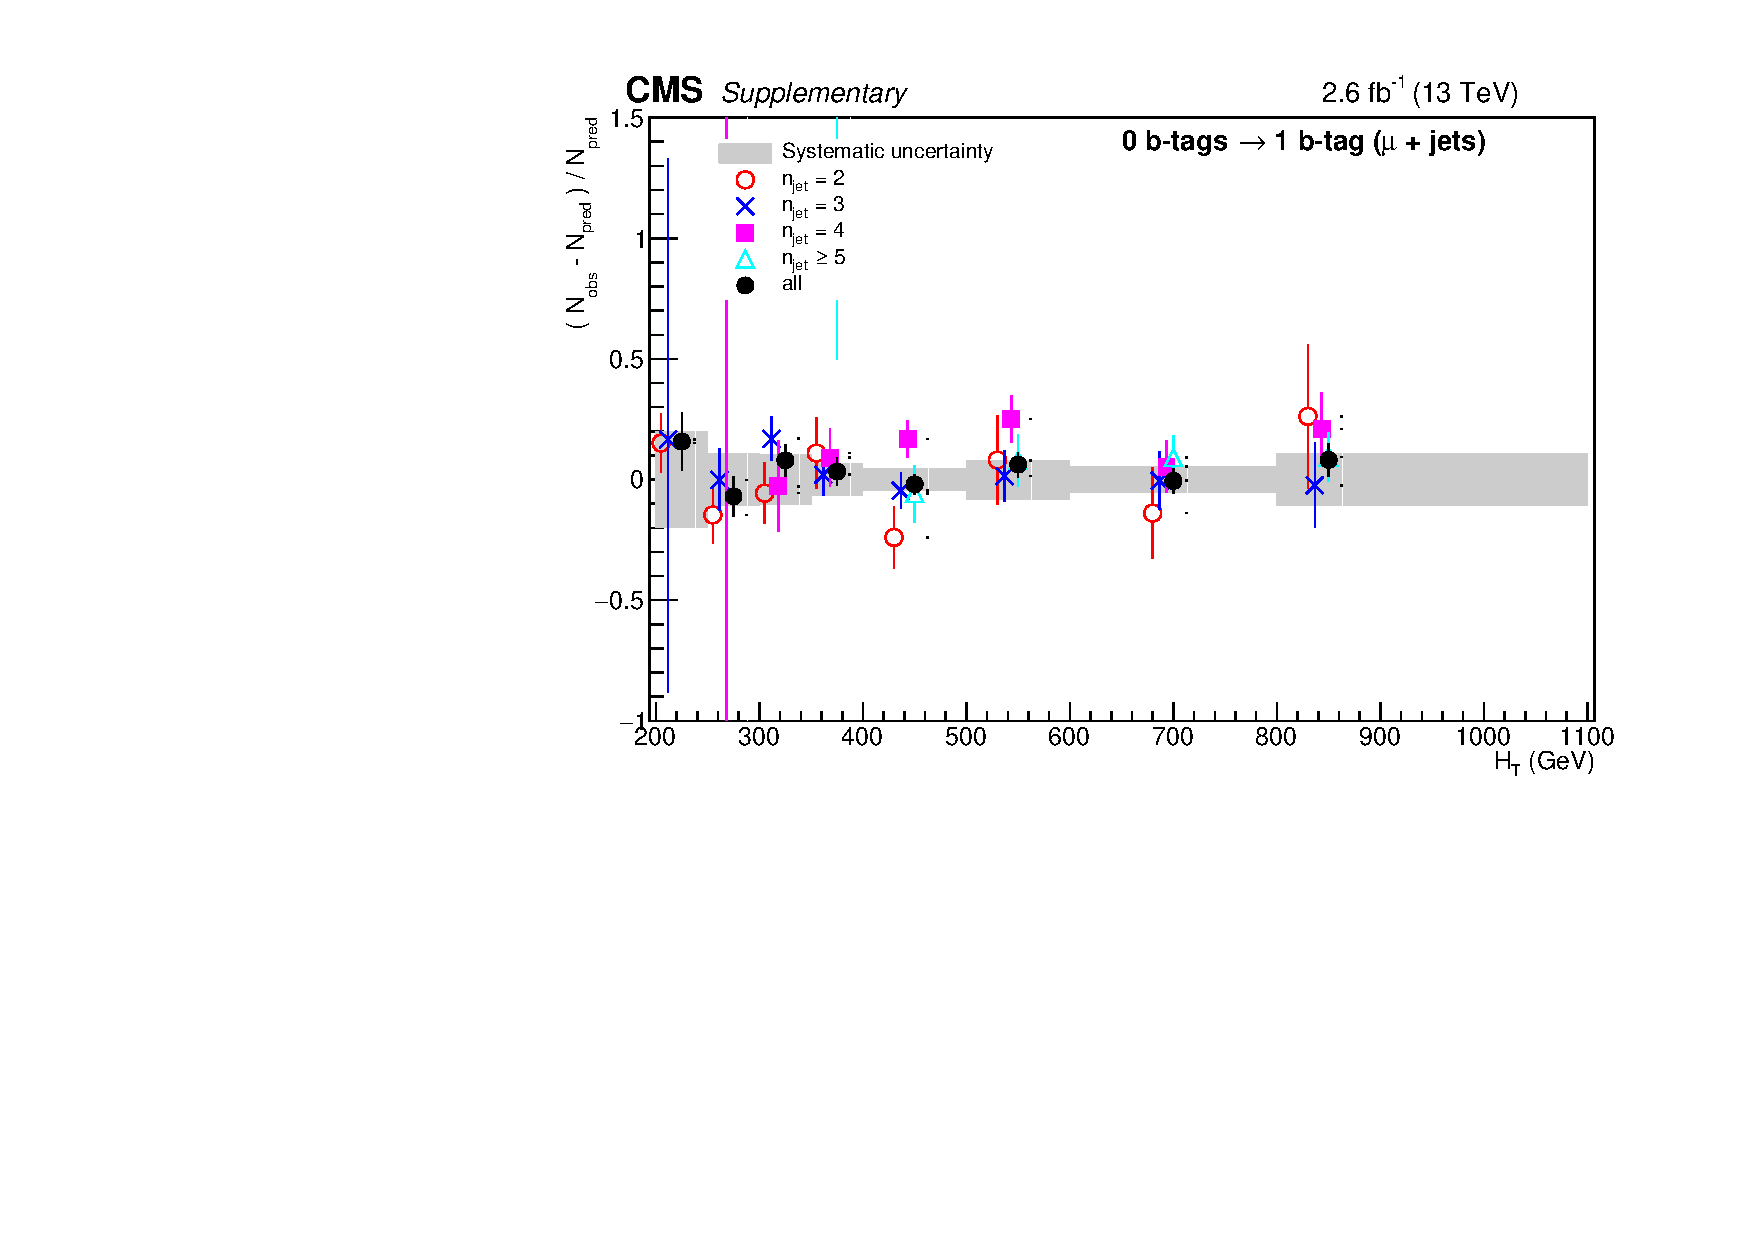
\includegraphics[width=0.7\textwidth]{figures/closureTests/eq0b_eq1b_muonsym__noFit.pdf}} \\
    ~~
    \subfigure[]{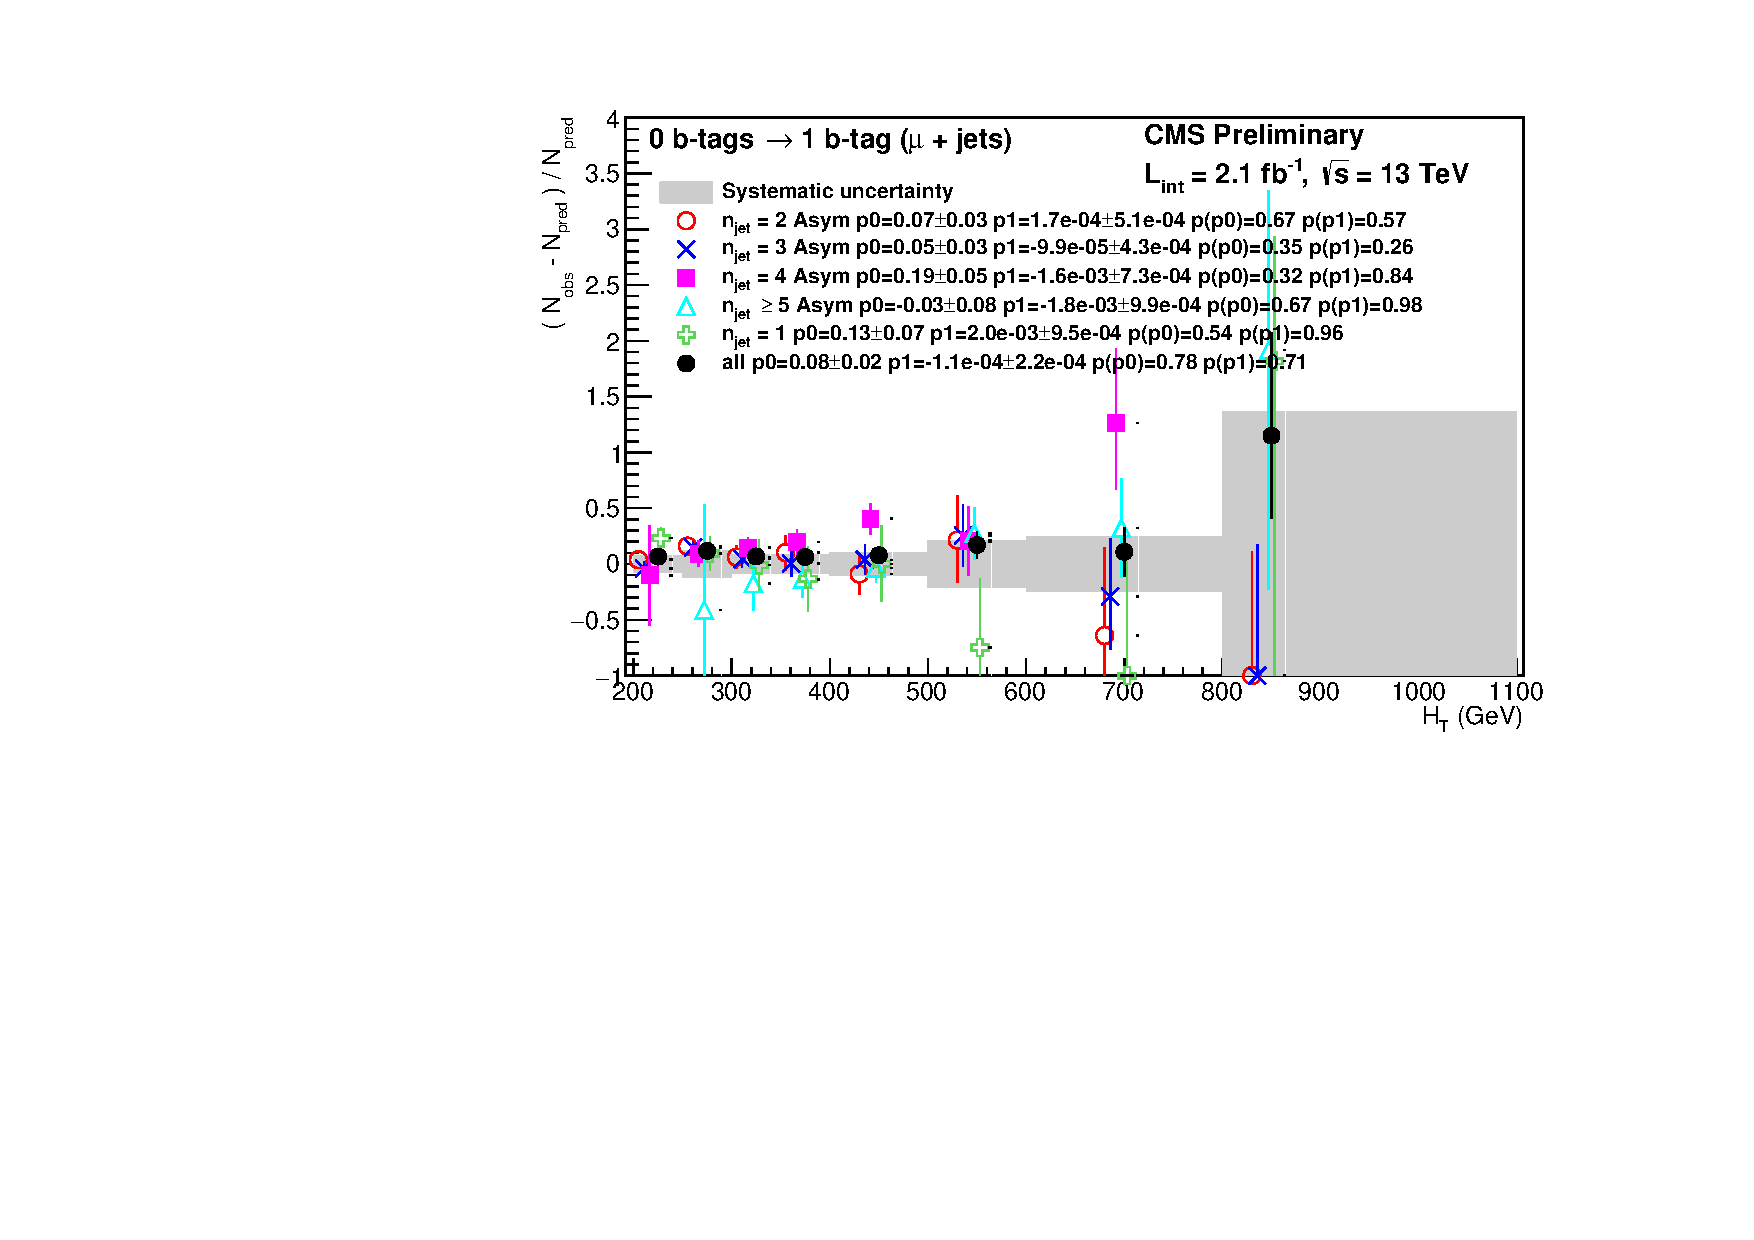
\includegraphics[width=0.7\textwidth]{figures/closureTests/eq0b_eq1b_muonasym__noFit.pdf}} 
    \caption{Data-driven tests probing the W and \ttbar admixture 
      in each \njet category (open symbols) overlaid on top of the systematic
      uncertainty estimates used for each of the seven \scalht bins
      (shaded bands), from formula method.
      The symmetric (asymmetric) jet topologies are shown in the top (bottom) plot.      
    }
    \label{fig:closureBTag-formula}
  \end{center} 
\end{figure}

\begin{figure}[!h]
  \centering
  \subfigure[b-tag SF up variation]{
    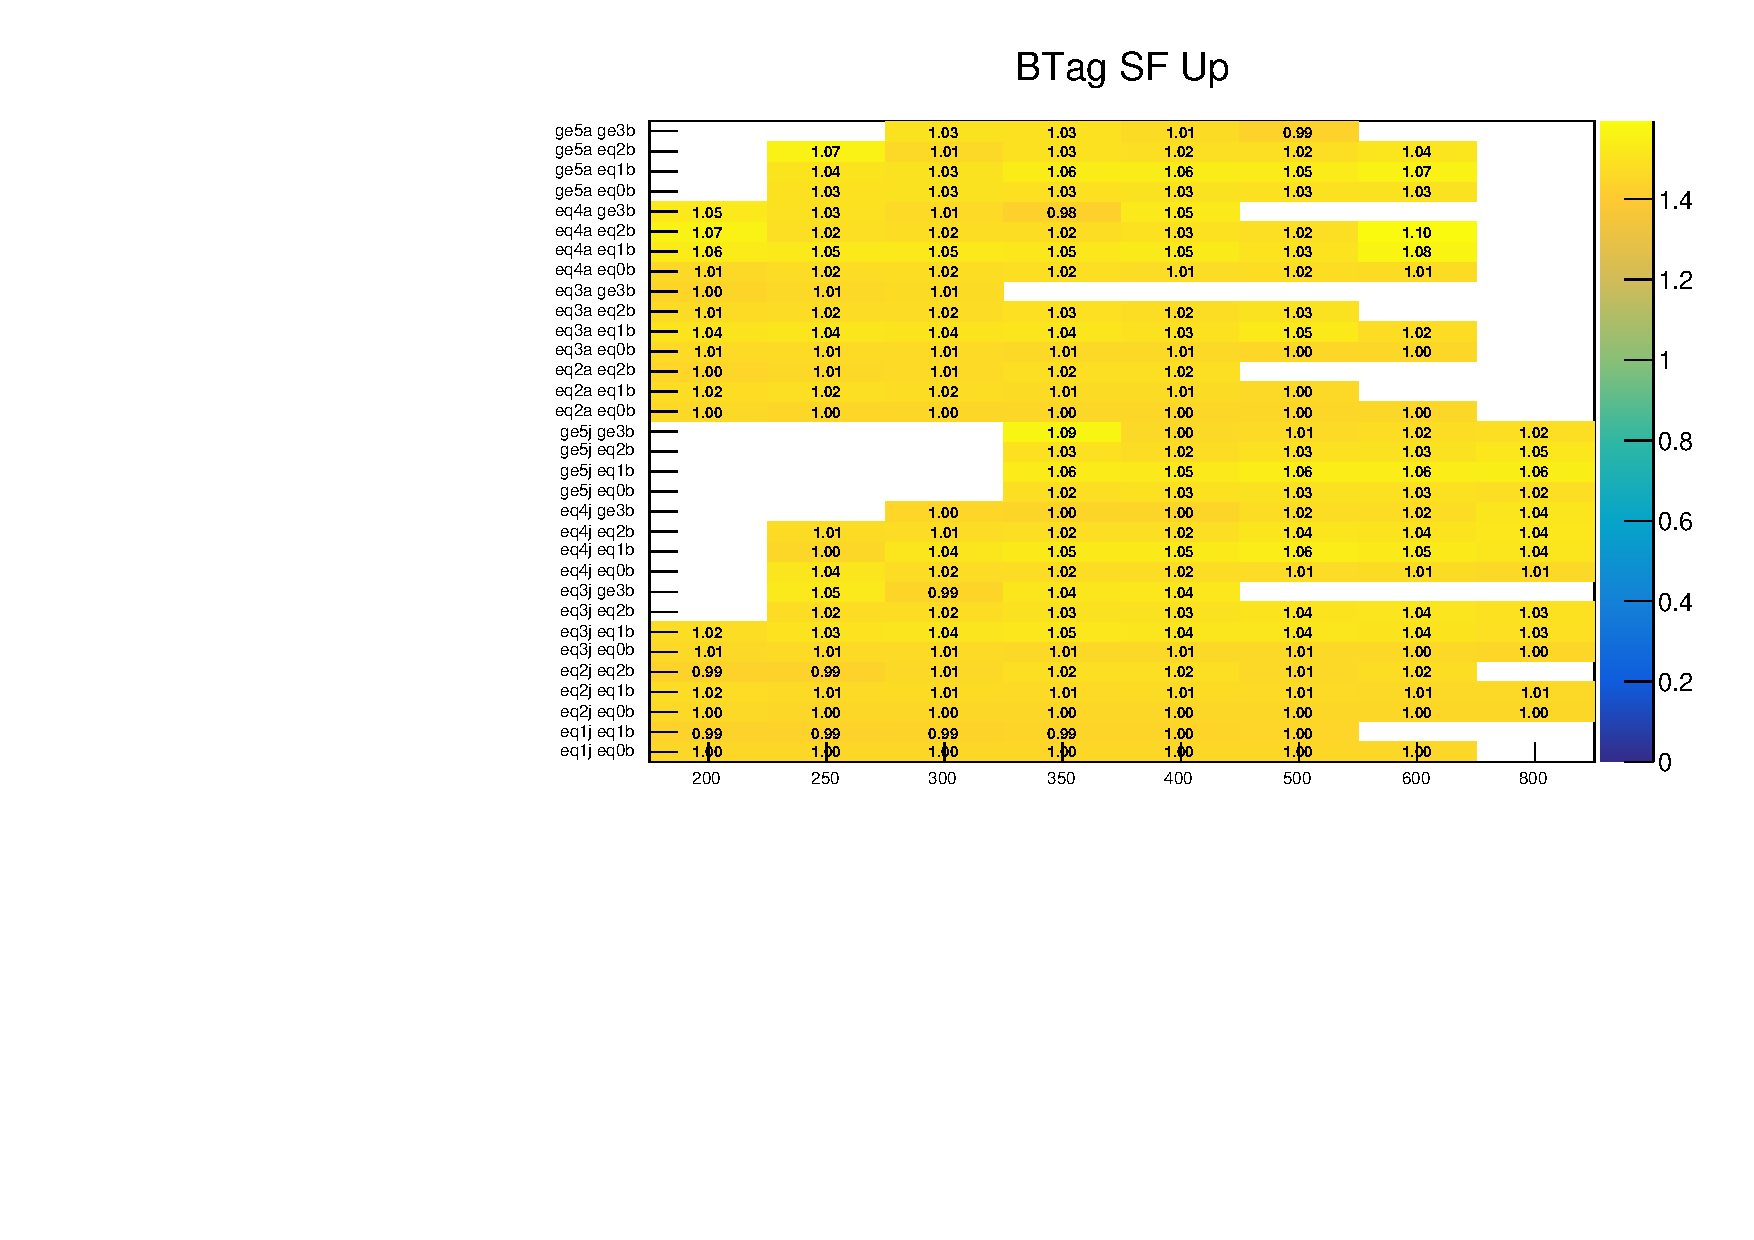
\includegraphics[width=0.5\textwidth]{figures/btagformula/Zinv_Mu/bsfWeight_UpRatio.pdf}
  } ~~
  \subfigure[b-tag SF down variation]{
    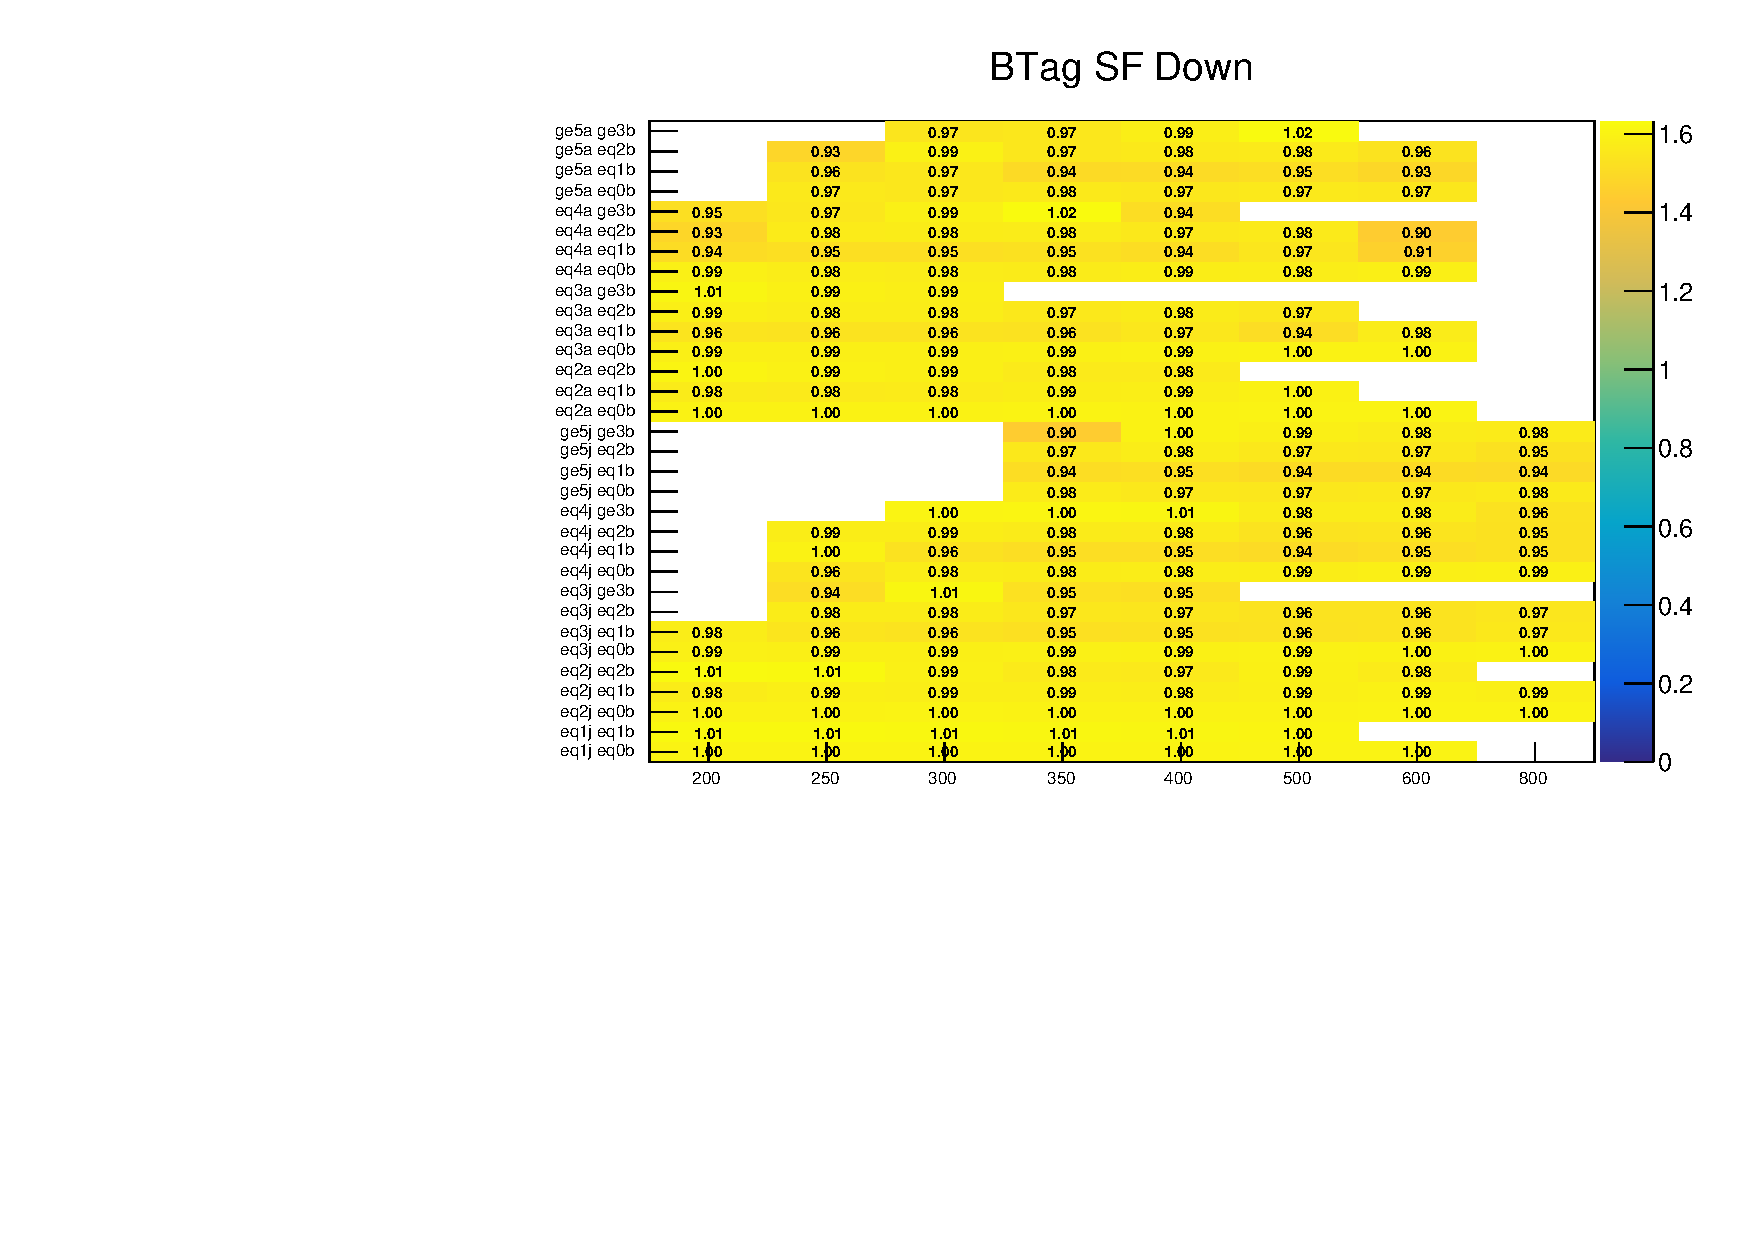
\includegraphics[width=0.5\textwidth]{figures/btagformula/Zinv_Mu/bsfWeight_DownRatio.pdf}
  }\\

  \caption{\label{fig:tfSyst_bsf_muToZinv-formula} The relative change in the
  $\mj \rightarrow (\znunu)$ transfer
  factors when varying b-tag SF in MC within its uncertainties, from formula method, 
  as a function of \scalht and jet category. 
  Variations corresponding to $+1\sigma$ ($-1\sigma$) are shown in the left (right) figure. 
  }
\end{figure}

\begin{figure}[!h]
  \centering
  \subfigure[b-tag SF up variation]{
    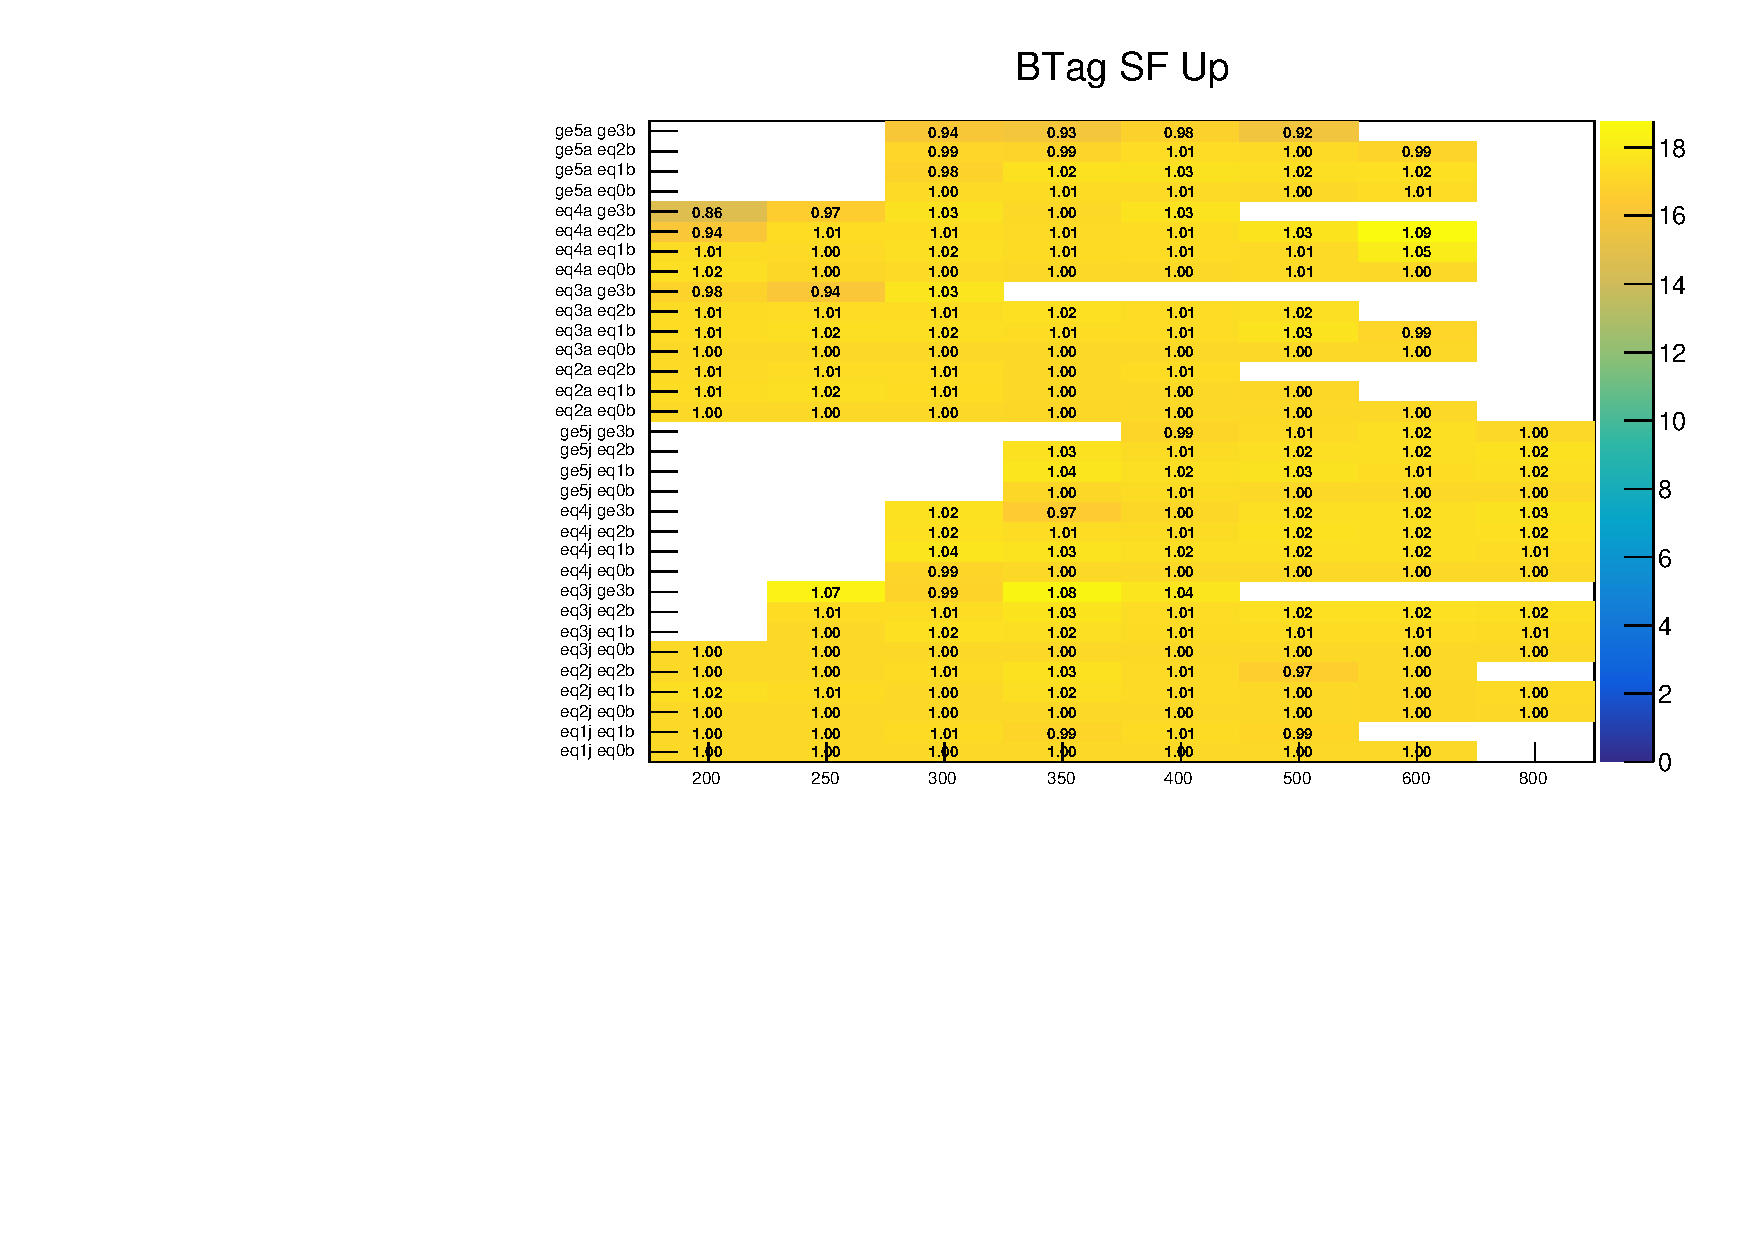
\includegraphics[width=0.5\textwidth]{figures/btagformula/Zinv_DiMu/bsfWeight_UpRatio.pdf}
  } ~~
  \subfigure[b-tag SF down variation]{
    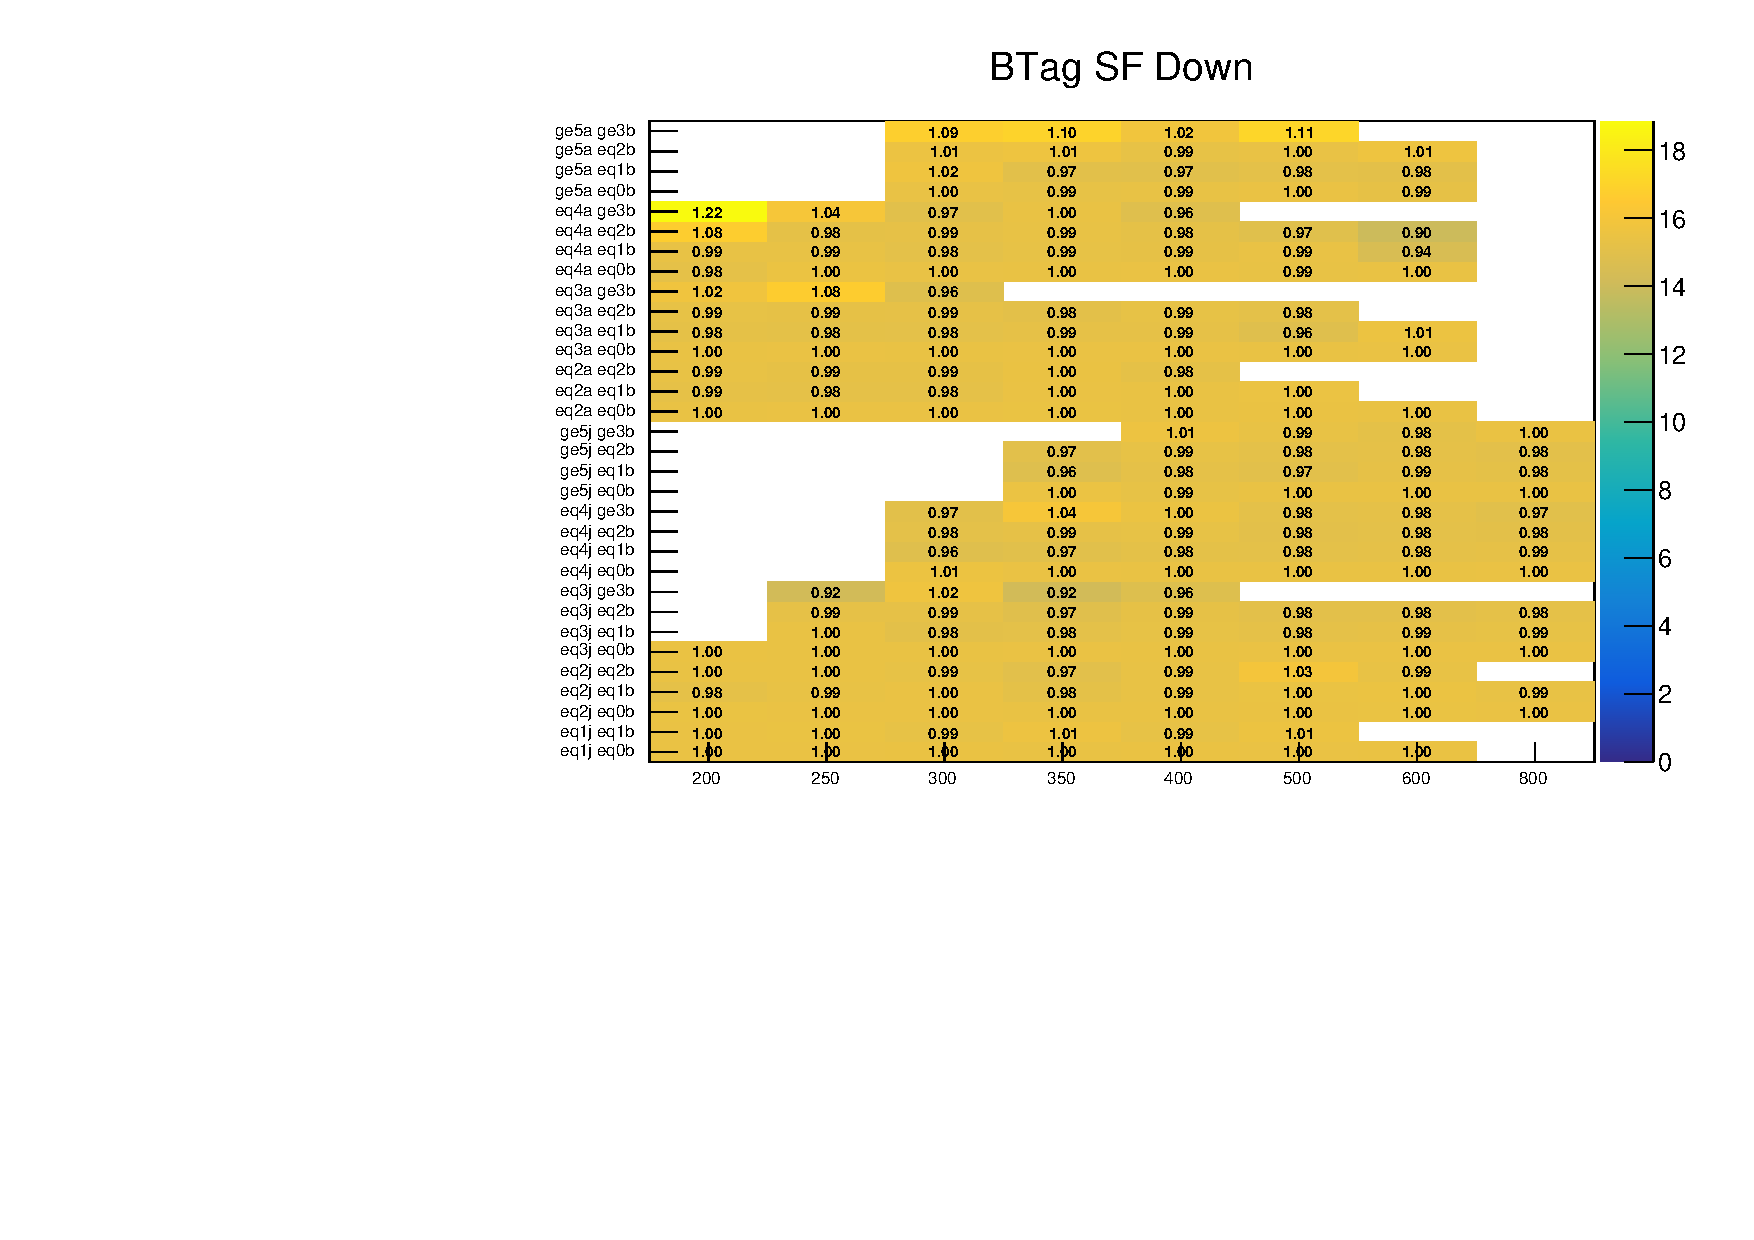
\includegraphics[width=0.5\textwidth]{figures/btagformula/Zinv_DiMu/bsfWeight_DownRatio.pdf}
  }\\

  \caption{\label{fig:tfSyst_bsf_mumuToZinv-formula} The relative change in
  the $\mmj \rightarrow (\znunu)$ transfer
  factors when varying b-tag SF in MC within its uncertainties, from formula method,
  as a function of \scalht and jet category. 
  Variations corresponding to $+1\sigma$ ($-1\sigma$) are shown in the left (right) figure. 
  }
\end{figure}

\begin{figure}[!h]
  \centering
  \subfigure[b-tag SF up variation]{
    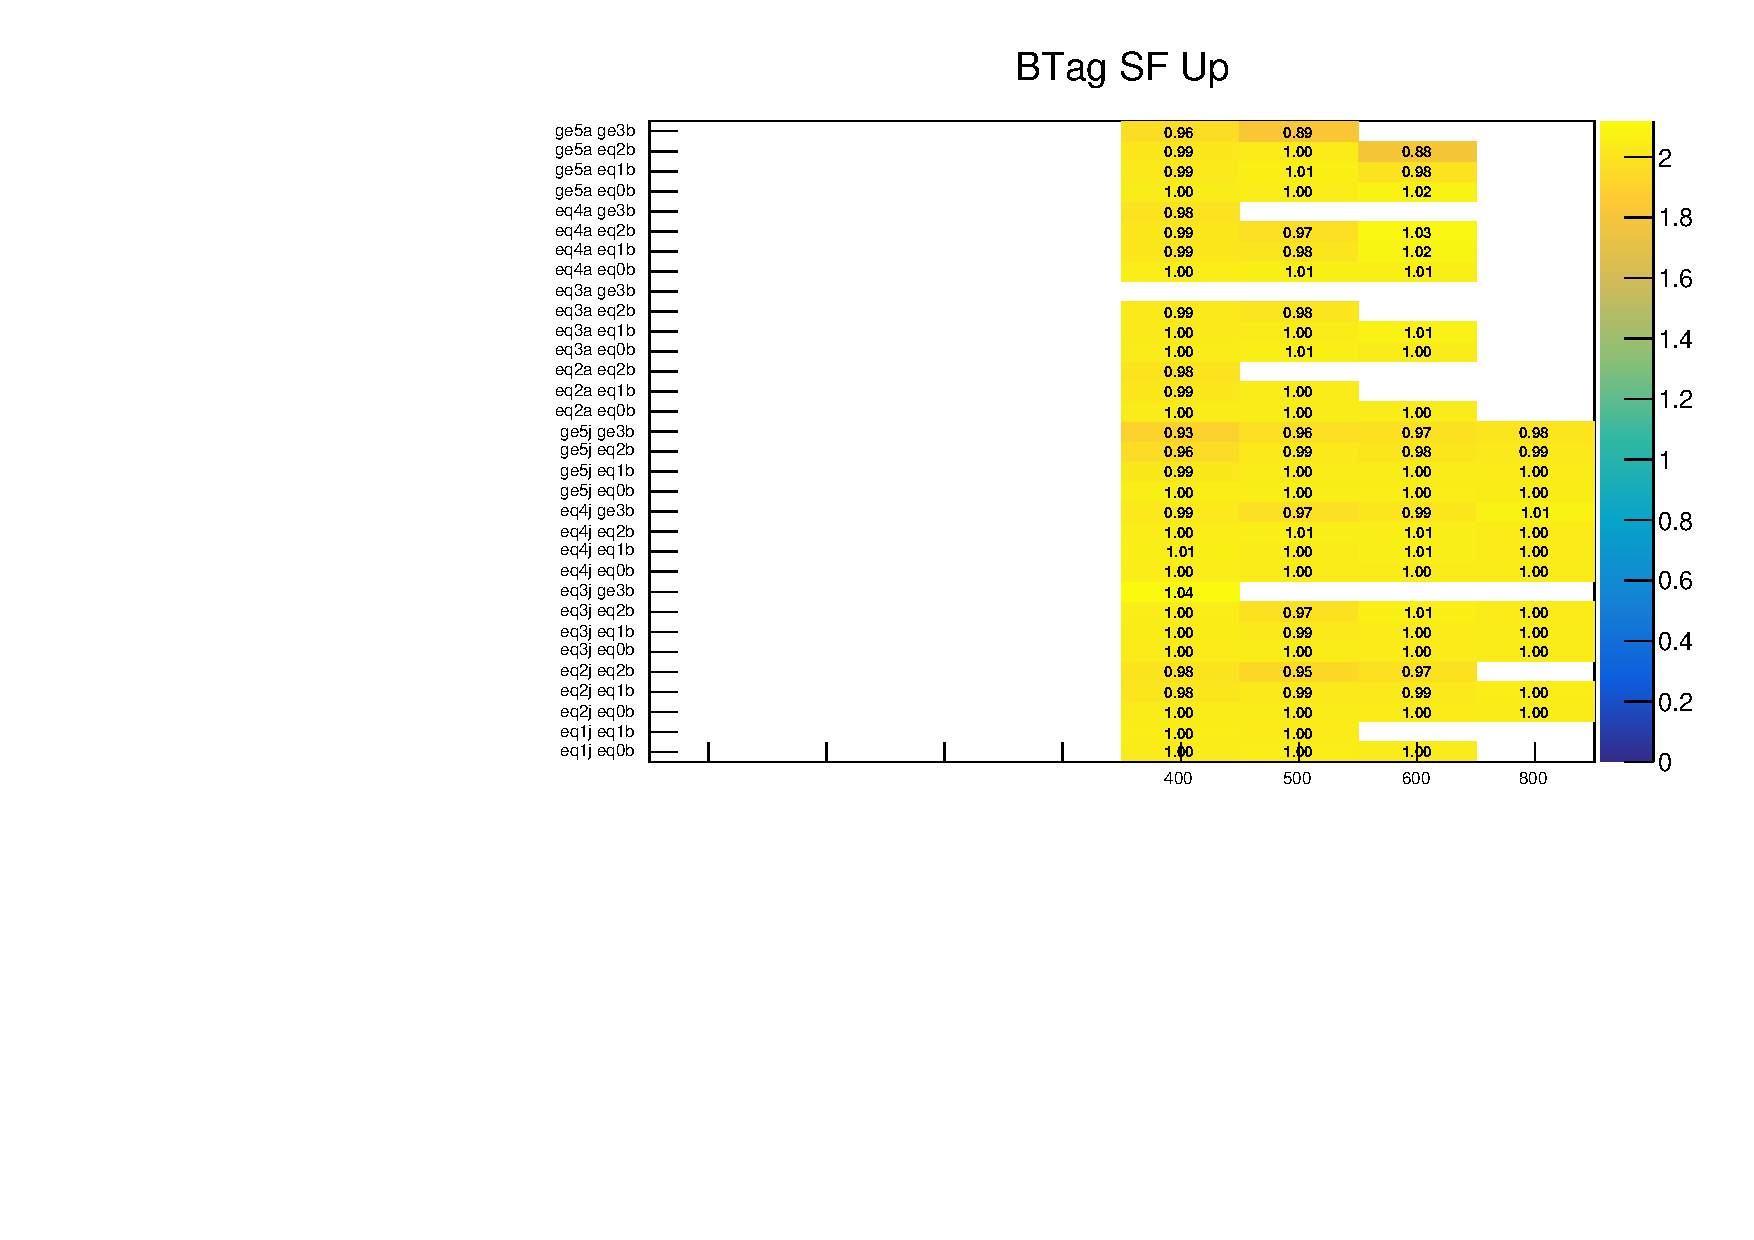
\includegraphics[width=0.5\textwidth]{figures/btagformula/Zinv_Pho/bsfWeight_UpRatio.pdf}
  } ~~
  \subfigure[b-tag SF down variation]{
    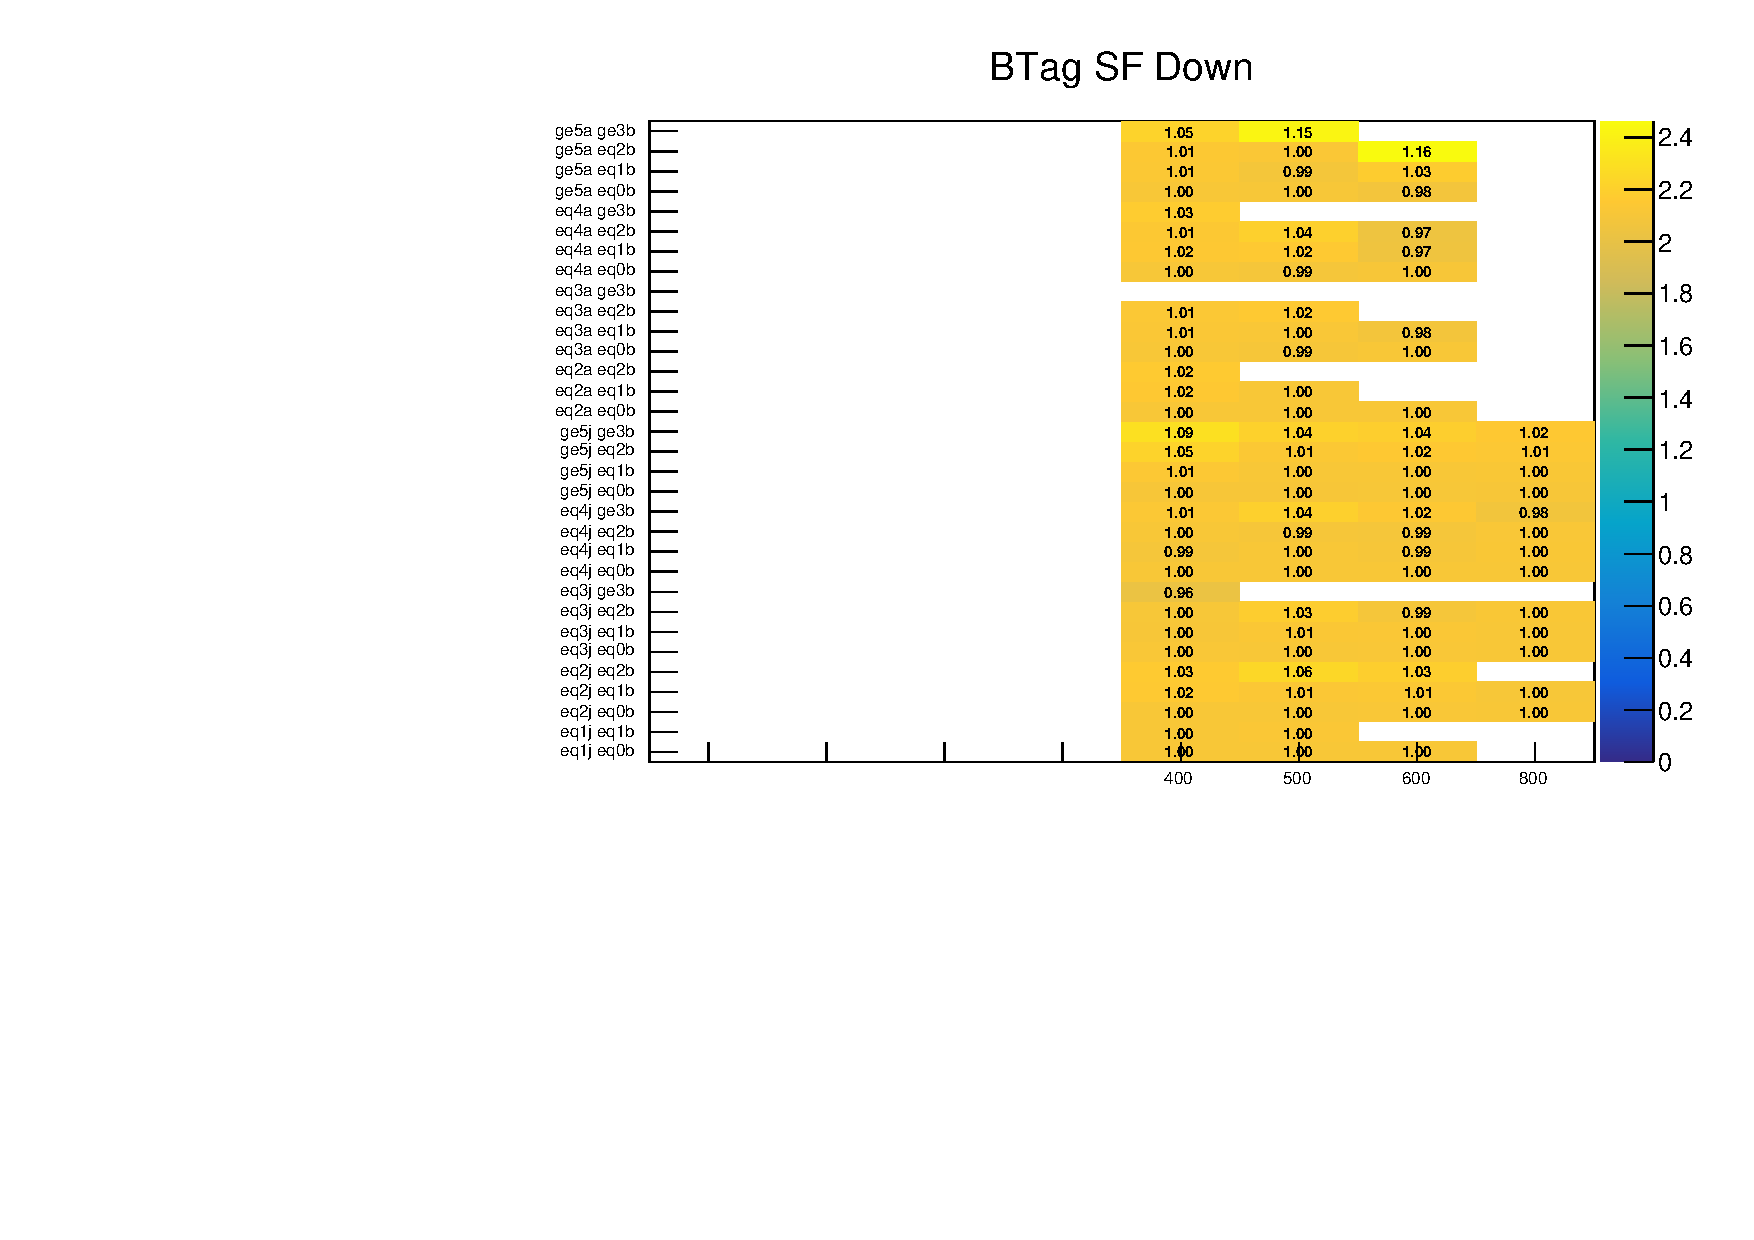
\includegraphics[width=0.5\textwidth]{figures/btagformula/Zinv_Pho/bsfWeight_DownRatio.pdf}
  }\\

  \caption{\label{fig:tfSyst_bsf_gjToZinv-formula} The relative change in the
  $\gj \rightarrow (\znunu)$ transfer
  factors when varying b-tag SF in MC within its uncertainties, from formula method, 
  as a function of \scalht and jet category. 
  Variations corresponding to $+1\sigma$ ($-1\sigma$) are shown in the left (right) figure. 
  }
\end{figure}

\begin{figure}[!h]
  \centering
  \subfigure[b-tag SF up variation]{
    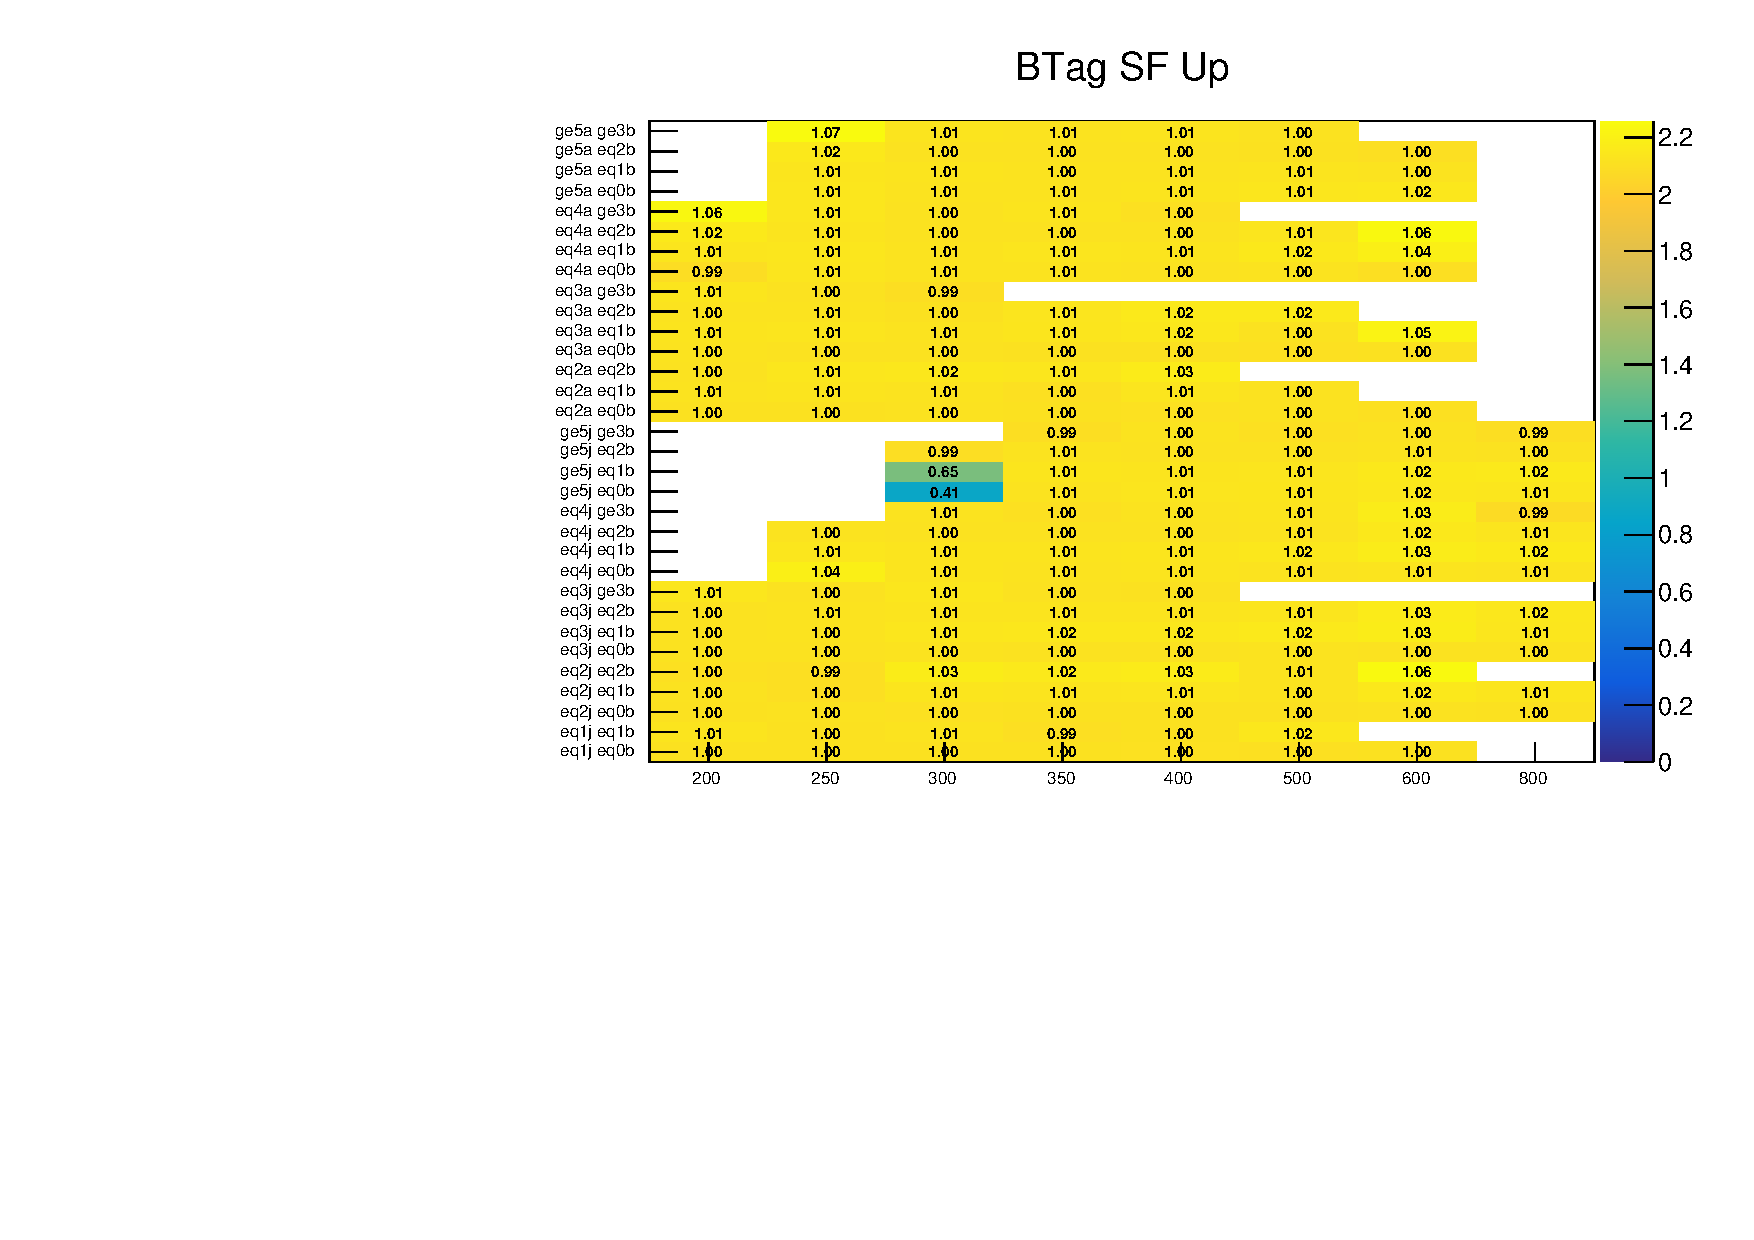
\includegraphics[width=0.5\textwidth]{figures/btagformula/Ttw_Mu/bsfWeight_UpRatio.pdf}
  } ~~
  \subfigure[b-tag SF down variation]{
    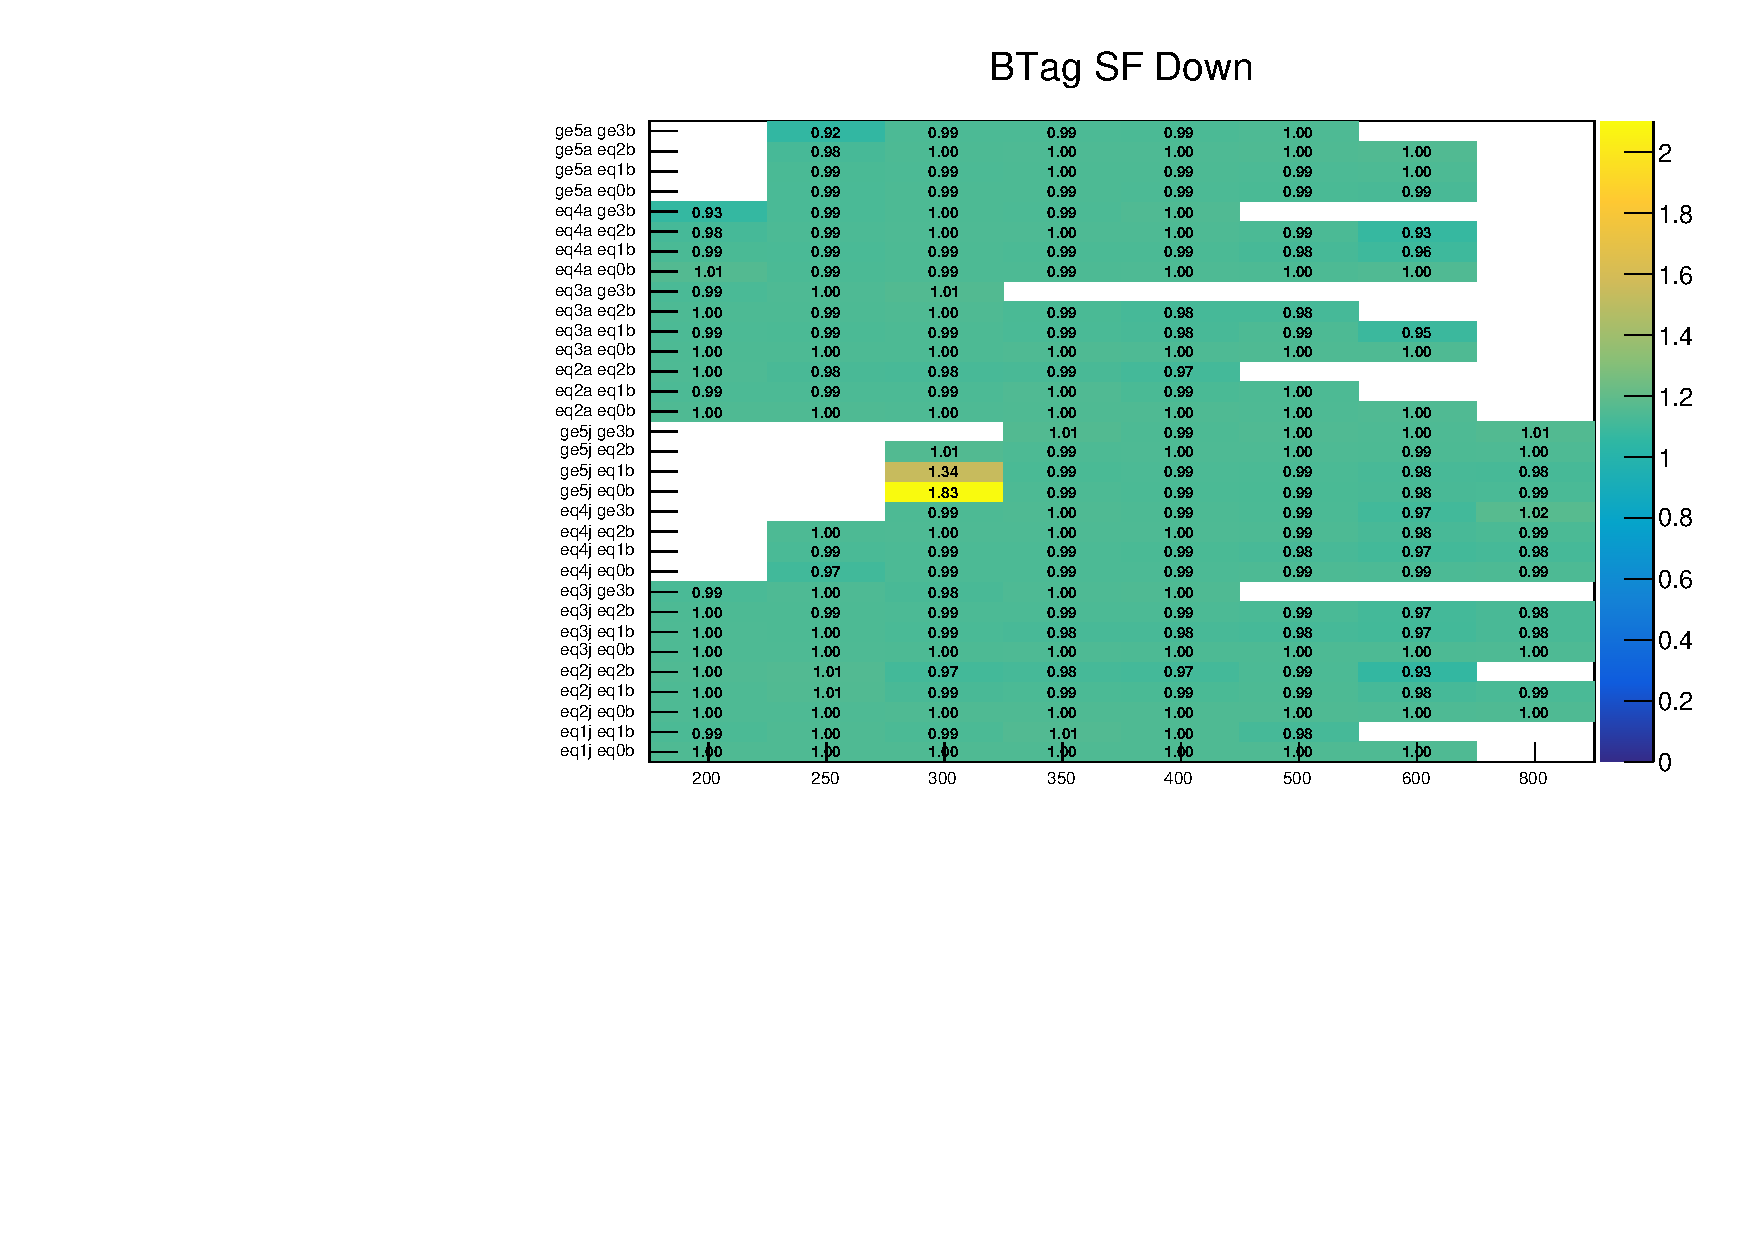
\includegraphics[width=0.5\textwidth]{figures/btagformula/Ttw_Mu/bsfWeight_DownRatio.pdf}
  }\\

  \caption{\label{fig:tfSyst_bsf_muToTtw-formula} The relative change in the $\mj \rightarrow \mathrm{tt+W}$ transfer
  factors when varying b-tag SF in MC within its uncertainties, from formula, 
  as a function of \scalht and jet category.
  Variations corresponding to $+1\sigma$ ($-1\sigma$) are shown in the left (right) figure. 
  }
\end{figure}


\subsection{Binning and systematic uncertainties in \mht dimension}
For a given (\njet, \nb,\scalht) bin, the threshold of the last \mht bin is 
motivated by a requirement on the statistic power in MC samples, i.e. statistical
uncertainty on this last bin to be less than 50\%. In bins with $n_{\rm b} \geq
3$, the formula method allows pushing the \mht threshold further given the
same requirement.

There are two components concerning the MC statistical uncertainties with 
the formula method: the MC statistical uncertainty from $N(n_{\textrm{b}}^{\textrm{gen}},
n_{\textrm{c}}^{\textrm{gen}}, n_{\textrm{l}}^{\textrm{gen}})$ in equation~\ref{equ:btag-formula}, and the 
MC statistical uncertainties from $\epsilon$, $f_{\rm c}$, and $f_{\rm light}$.
The former uncertainty is the same across the \nb~dimension, for each (\njet,
~\scalht,~\mht) bin. The later uncertainty is determined for each $n_{\rm b}$, by 
varying $\epsilon$, $f_{\rm c}$, and $f_{\rm light}$ up and down within their 
statistical error. The two statistical uncertainties are then added in quadrature for each 
(\njet,~\nb,~\scalht,~\mht) bin. The last \mht bin is required to have such
 statistical uncertainty $< 50\%$ for the EWK component.

The statistical uncertainty mentioned above are used to 
build alternative \mht templates, correlated across the \nb~dimension, 
and it is taken as an extra source of systematics in Section~\ref{sec:mcSystStudiesShape}.

Figure~\ref{fig:mhtShape_Ewk_ge5j_ge3b_ht800} compares the \mht distribution from
the formula method and raw MC, in one of the most sensitive bins in the analysis and Figure~\ref{fig:mhtShapeErr_Ewk_ge5j_ge3b_ht800} compares the associated 
 statistical uncertainties. Reduced uncertainties show better control 
  of extreme \mht tail in high \nb~bins.

Figure~\ref{fig:lastMhtBin} shows thresholds on last \mht bins for each (\njet,
~\nb,~\scalht) category, with the criterion defined above.


\begin{figure}[h!]
  \centering
  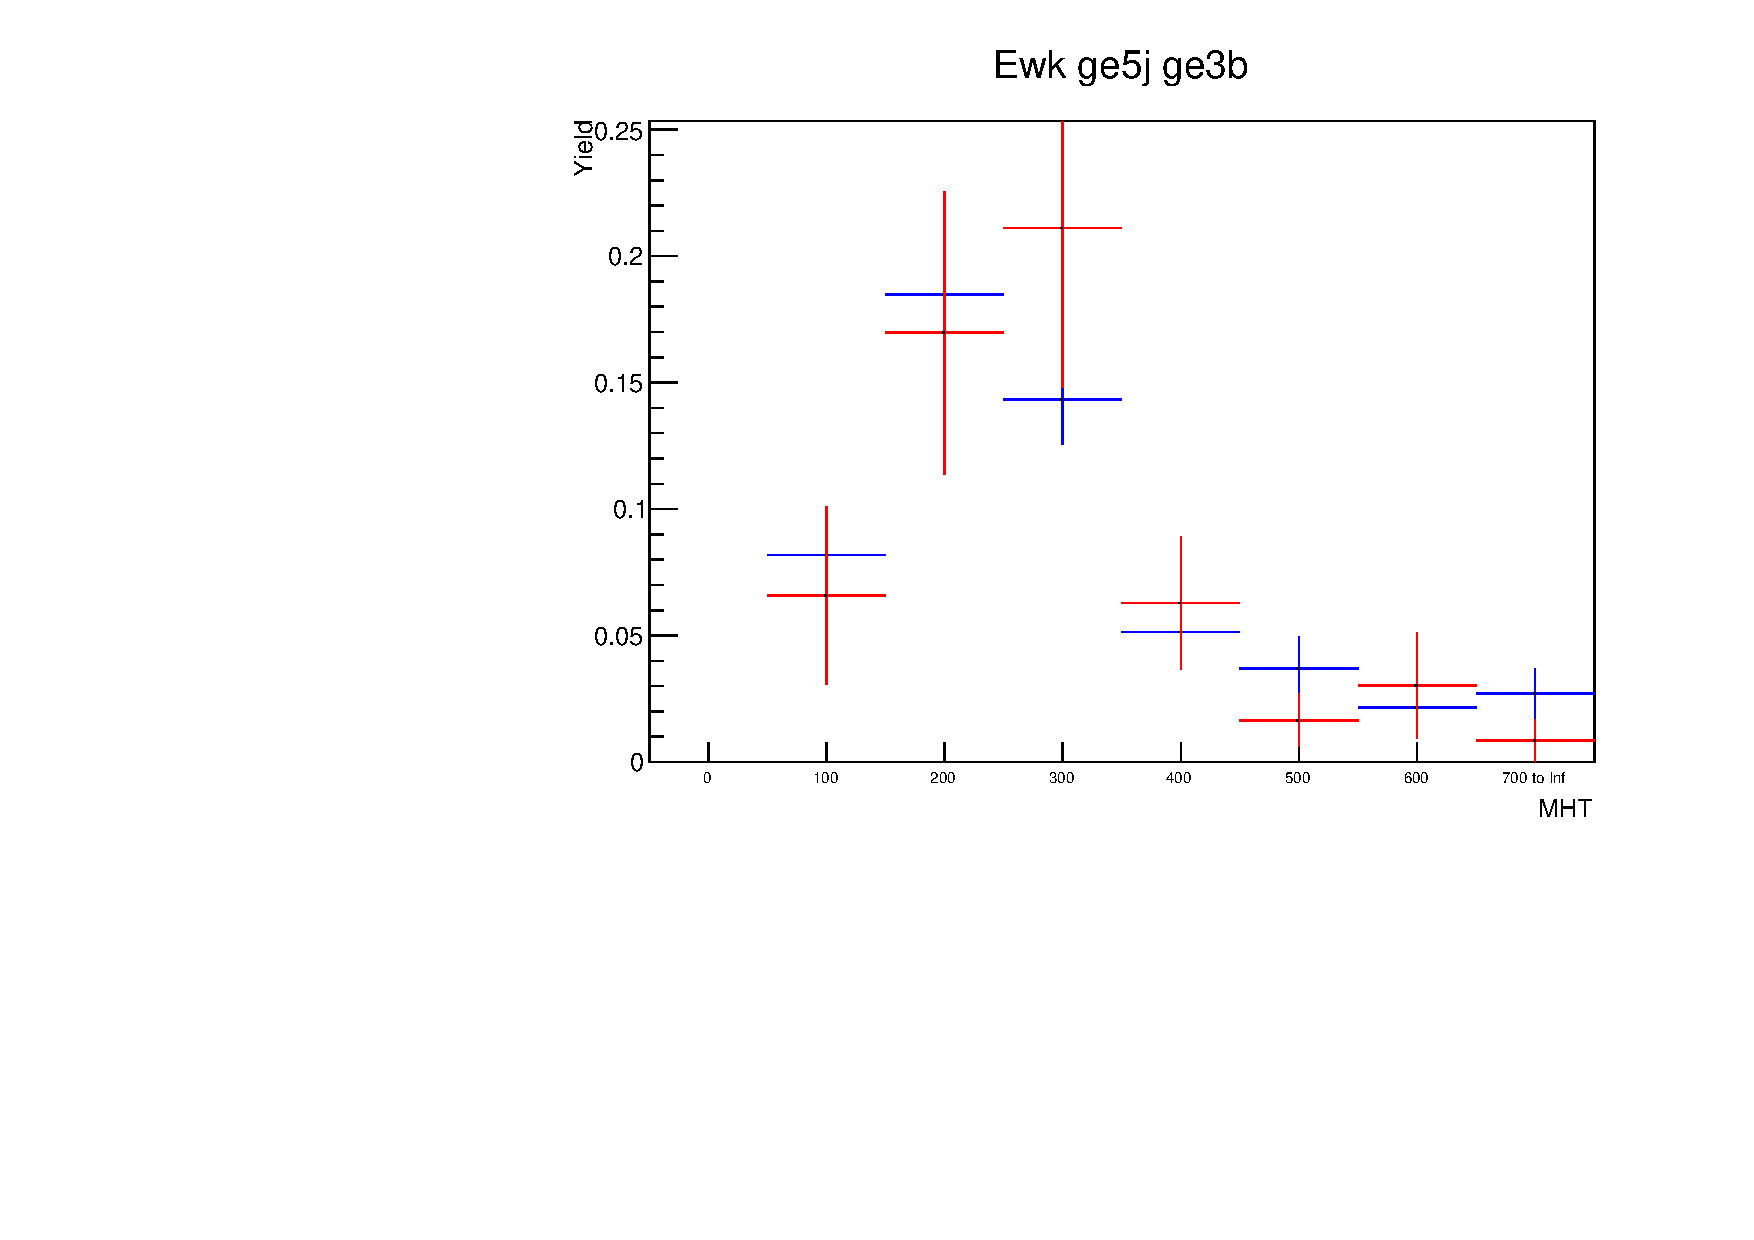
\includegraphics[width=0.7\textwidth]{figures/btagformula/GoodMHTShape_ge5j_ge3b.pdf} 
  \caption{\label{fig:mhtShape_Ewk_ge5j_ge3b_ht800} \mht distribution from formula
   method (Blue) and raw MC (Red) for the bin \scalht $800-\infty$, \njet $\geq 5$, \nb $\geq 3$.}
\end{figure}

\begin{figure}[h!]
  \centering
  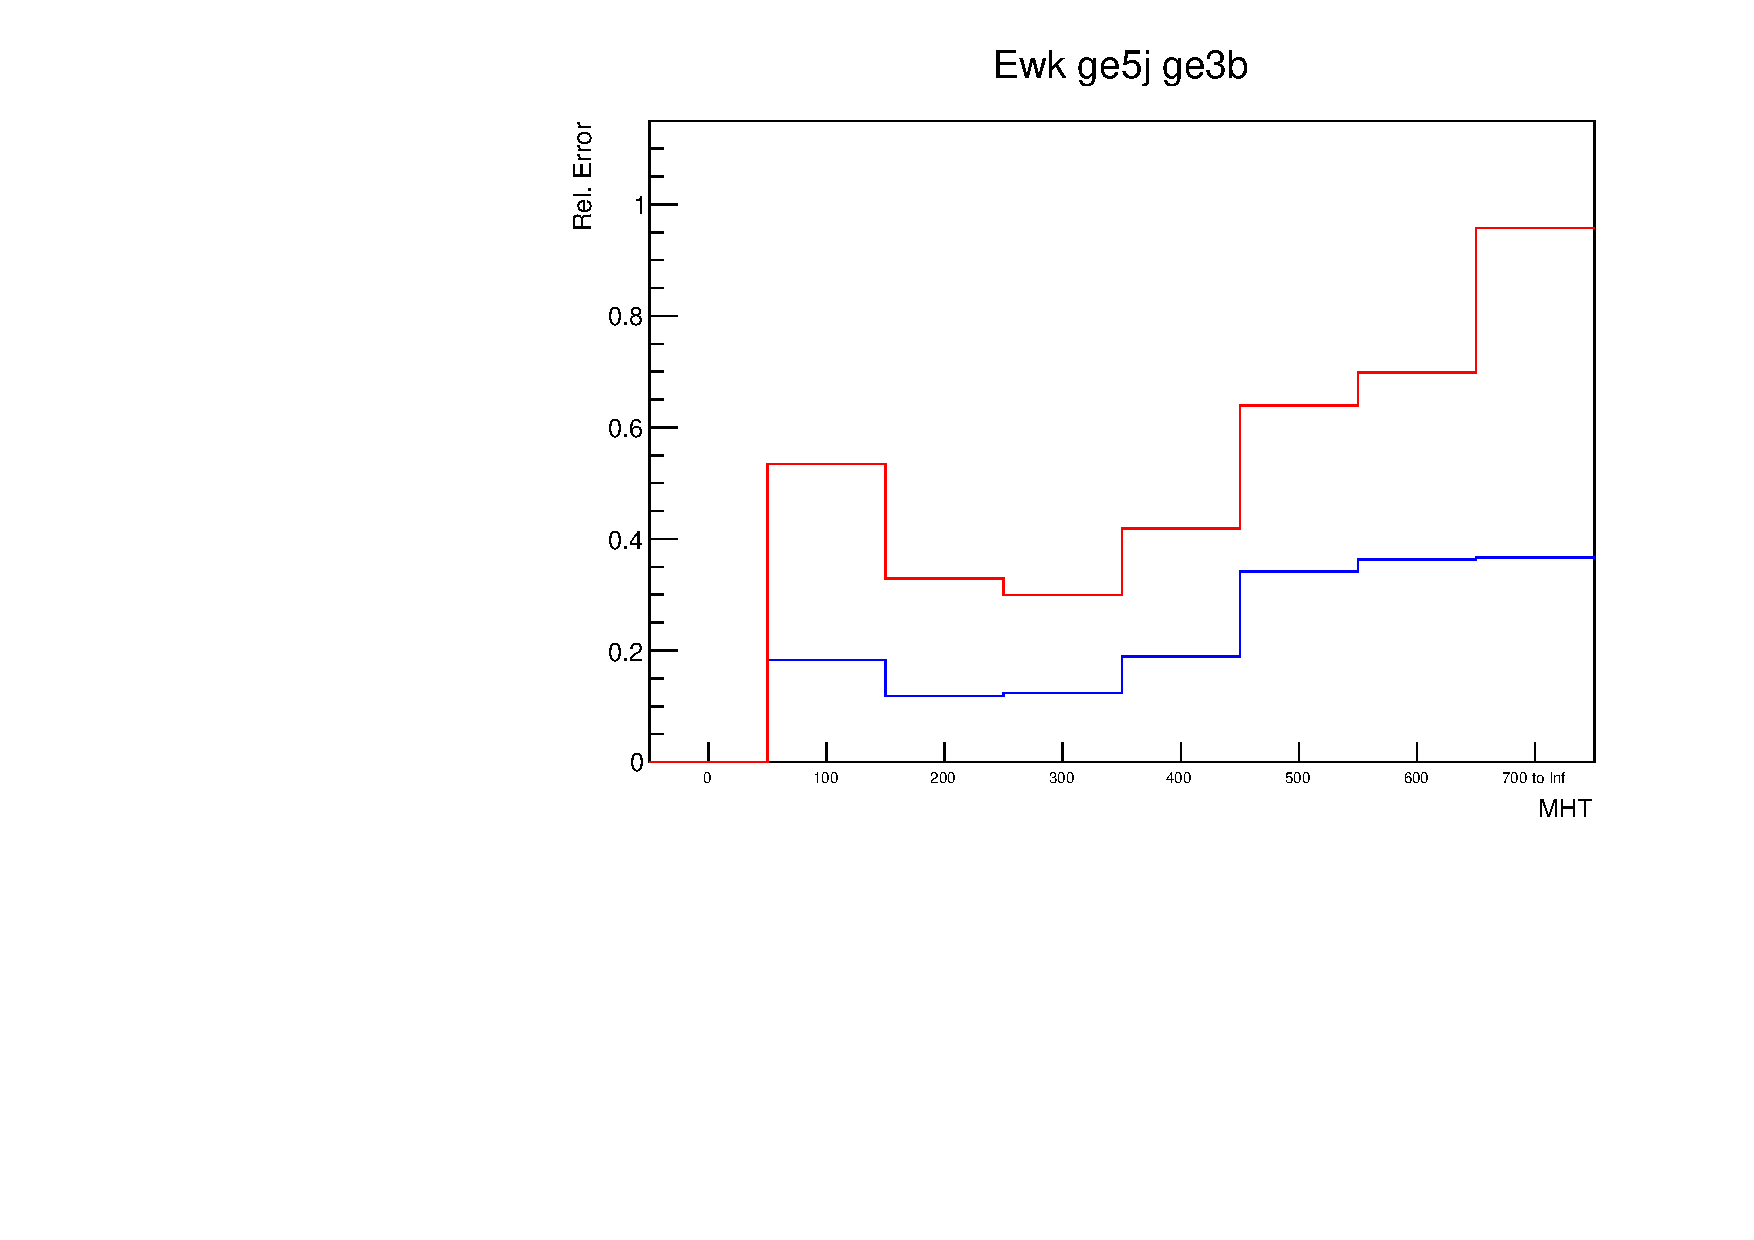
\includegraphics[width=0.7\textwidth]{figures/btagformula/GoodMHTShapeErr_ge5j_ge3b.pdf} 
  \caption{\label{fig:mhtShapeErr_Ewk_ge5j_ge3b_ht800} Statistical uncertainty on \mht 
  distribution from formula method (Blue) and raw MC (Red) for the bin
  \scalht $800-\infty$, \njet $\geq 5$, \nb $\geq 3$.}
\end{figure}

\begin{figure}[h!]
  \centering
  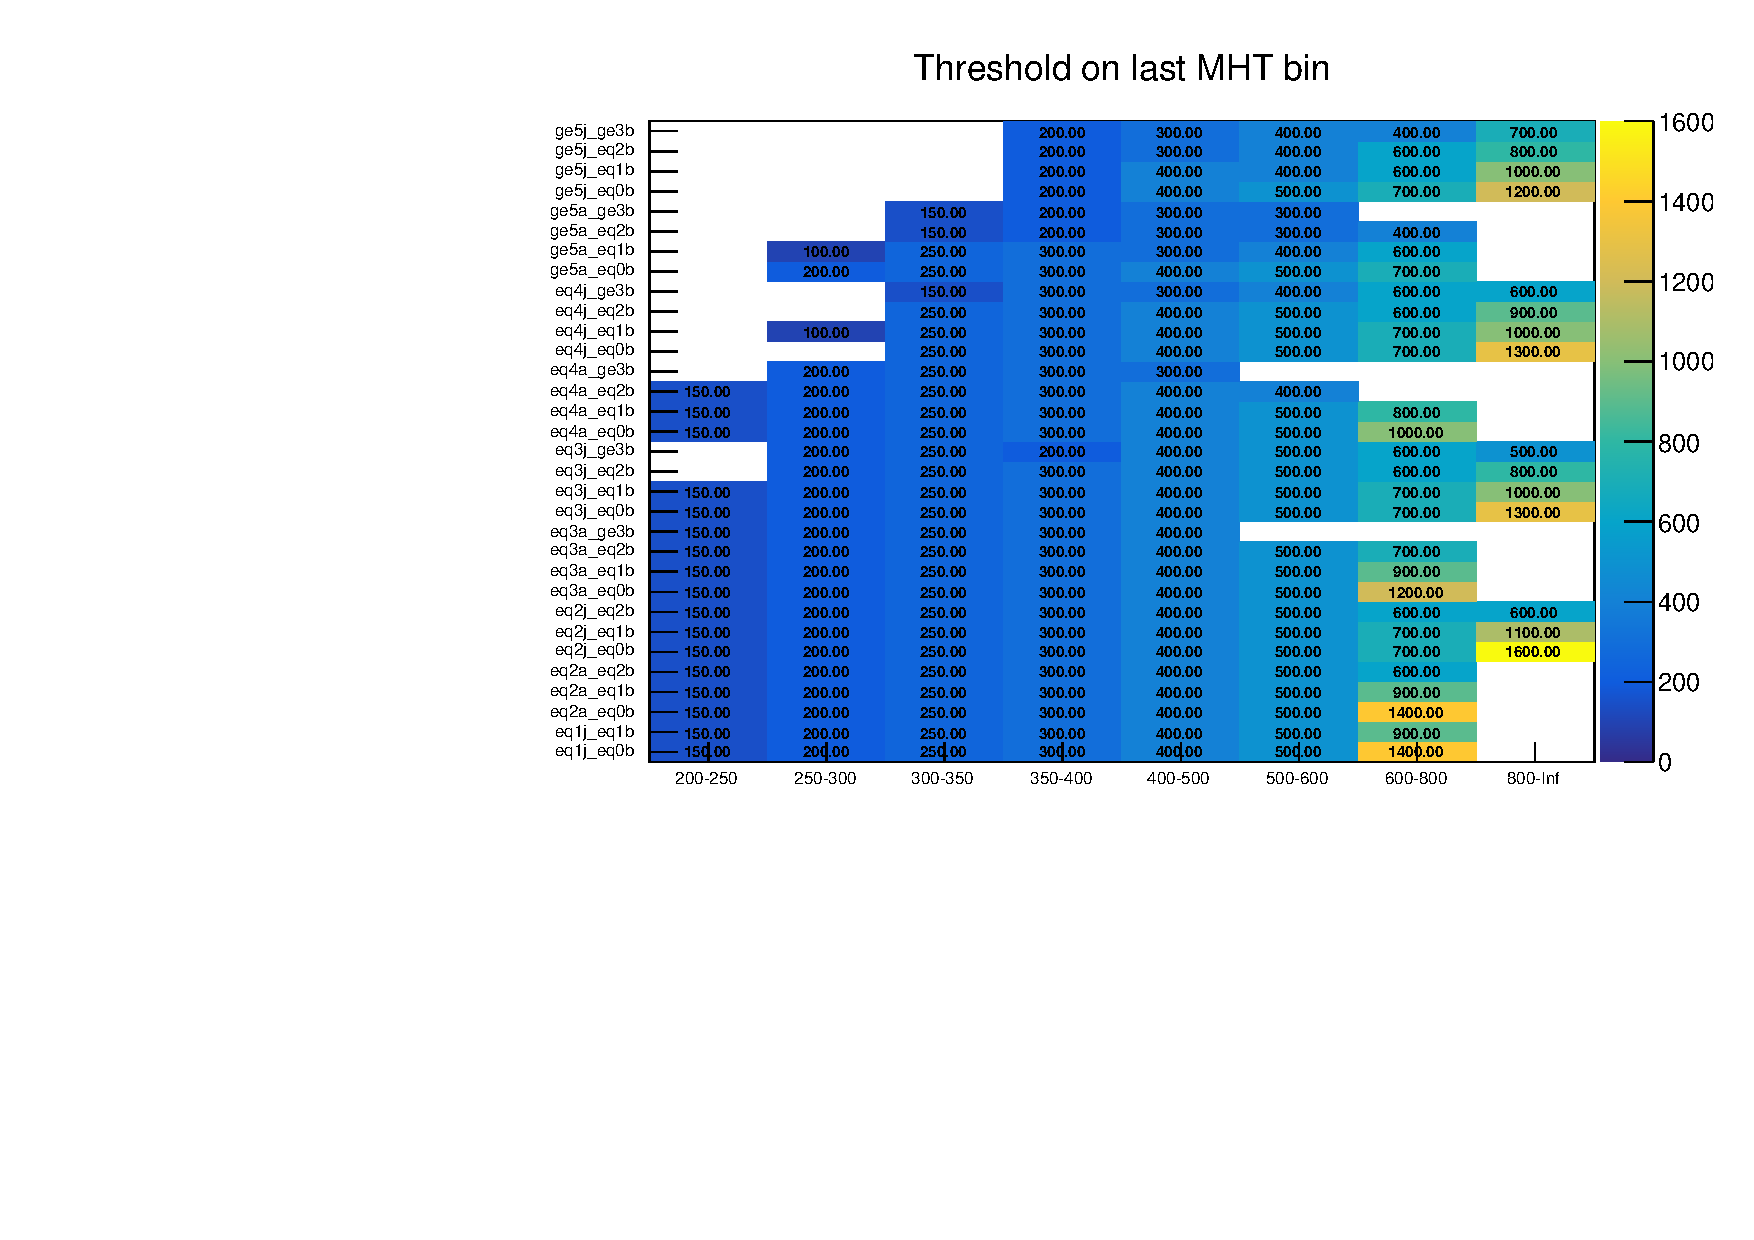
\includegraphics[width=0.8\textwidth]{figures/btagformula/Ewk_lastMhtBin.pdf} 
  \caption{\label{fig:lastMhtBin} Thresholds on last \mht bin for each (\njet,
  ~\nb,~\scalht) category}
\end{figure}


\subsection{Performance}
The formula method brings extra sensitivity to a wide range of SUSY models with final
states enriched in b-jets.
Especially it enhances the statistical power in bins dominated by the backgrounds 
with mis-tagging, because mis-tagged rates are generally much smaller than 
btagging efficiency. The sensitivity of the analysis with the formula method is 
tested by comparing expected significances with formula method and raw MC, 
at 8~\ifb. The test is performed with \mht binning of 100 \gev bin 
width, with last \mht bin being $800-\infty$.

Table~\ref{tab:t1bbbb-formula-8fb},~\ref{tab:t1tttt-formula-8fb},
~\ref{tab:t1ttbb-formula-8fb},~\ref{tab:t2tt-formula-8fb},~\ref{tab:t5ttcc-formula-8fb} 
show expected significances for some benchmark models for 5 SUSY models, T1bbbb, 
T1tttt, T1ttbb, T2tt and T5ttcc. General improvements, in range of 10\% to 30\%
 are observed, prominently in uncompressed scenarios. There are a few slight 
 degradation due to shifted background central values.

%
\definecolor{Red}{rgb}{1,0,0}
\begin{longtable}{| c | c | c | c  | }
\caption{Expected significance for various T1bbbb models at 2.2~\ifb} \label{tab:t1bbbb-formula-2p2fb} \\    \hline 
Signal Model & Formula & Standard & Improvement\\ \hline 
$m_{\mathrm{Susy}} = 1400 \gev ,m_{\mathrm{LSP}} 1000 \gev$  & 2.70 & 2.75 & -0.02\\ \hline 
$m_{\mathrm{Susy}} = 1400 \gev ,m_{\mathrm{LSP}} 100  \gev$ & 4.43 & 4.15 & 0.07\\ \hline 
$m_{\mathrm{Susy}} = 1400 \gev ,m_{\mathrm{LSP}} 800  \gev$ & 4.05 & 4.11 & -0.01\\ \hline 
$m_{\mathrm{Susy}} = 1500 \gev ,m_{\mathrm{LSP}} 1000 \gev$  & 2.26 & 2.36 & -0.04\\ \hline 
$m_{\mathrm{Susy}} = 1500 \gev ,m_{\mathrm{LSP}} 100  \gev$ & 3.21 & 2.95 & 0.09\\ \hline 
$m_{\mathrm{Susy}} = 1500 \gev ,m_{\mathrm{LSP}} 800  \gev$ & 3.08 & 3.09 & -0.00\\ \hline 
$m_{\mathrm{Susy}} = 1600 \gev ,m_{\mathrm{LSP}} 1000 \gev$  & 1.86 & 1.91 & -0.03\\ \hline 
$m_{\mathrm{Susy}} = 1600 \gev ,m_{\mathrm{LSP}} 100  \gev$ & 2.22 & 1.97 & 0.13\\ \hline 
$m_{\mathrm{Susy}} = 1600 \gev ,m_{\mathrm{LSP}} 800  \gev$ & 2.22 & 2.19 & 0.02\\ \hline 
$m_{\mathrm{Susy}} = 1700 \gev ,m_{\mathrm{LSP}} 1000 \gev$  & 1.41 & 1.42 & -0.01\\ \hline 
$m_{\mathrm{Susy}} = 1700 \gev ,m_{\mathrm{LSP}} 100  \gev$ & 1.53 & 1.31 & 0.17\\ \hline 
$m_{\mathrm{Susy}} = 1700 \gev ,m_{\mathrm{LSP}} 800  \gev$ & 1.66 & 1.56 & 0.06\\ \hline 
$m_{\mathrm{Susy}} = 1800 \gev ,m_{\mathrm{LSP}} 1000 \gev$  & 1.02 & 0.98 & 0.04\\ \hline 
$m_{\mathrm{Susy}} = 1800 \gev ,m_{\mathrm{LSP}} 100  \gev$ & 1.06 & 0.87 & 0.22\\ \hline 
$m_{\mathrm{Susy}} = 1800 \gev ,m_{\mathrm{LSP}} 800  \gev$ & 1.14 & 1.03 & 0.11\\ \hline 
    \hline 
    \hline 
\end{longtable}


\begin{figure}

\definecolor{Red}{rgb}{1,0,0}
\begin{longtable}{| c | c | c | }%c | }
\caption{Expected significance for various T1bbbb models at 8~\ifb} \label{tab:t1bbbb-formula-8fb} \\    \hline 
Signal Model & Formula & Standard \\ \hline 
$m_{\mathrm{Susy}} = 1400 \gev ,m_{\mathrm{LSP}} = 1000 \gev$  	& 5.31 	& 5.20 \\ \hline	%& 0.02\\ \hline 
$m_{\mathrm{Susy}} = 1400 \gev ,m_{\mathrm{LSP}} = 100  \gev$ 	& 8.57 	& 7.65 \\ \hline	%& 0.12\\ \hline 
$m_{\mathrm{Susy}} = 1400 \gev ,m_{\mathrm{LSP}} = 800  \gev$ 	& 7.94 	& 7.75 \\ \hline	%& 0.03\\ \hline 
$m_{\mathrm{Susy}} = 1500 \gev ,m_{\mathrm{LSP}} = 1000 \gev$  	& 4.46 	& 4.51 \\ \hline	%& -0.01\\ \hline 
$m_{\mathrm{Susy}} = 1500 \gev ,m_{\mathrm{LSP}} = 100  \gev$ 	& 6.23 	& 5.44 \\ \hline	%& 0.15\\ \hline 
$m_{\mathrm{Susy}} = 1500 \gev ,m_{\mathrm{LSP}} = 800  \gev$ 	& 6.05 	& 5.83 \\ \hline	%& 0.04\\ \hline 
$m_{\mathrm{Susy}} = 1600 \gev ,m_{\mathrm{LSP}} = 1000 \gev$  	& 3.66 	& 3.63 \\ \hline	%& 0.01\\ \hline 
$m_{\mathrm{Susy}} = 1600 \gev ,m_{\mathrm{LSP}} = 100  \gev$ 	& 4.33 	& 3.60 \\ \hline	%& 0.20\\ \hline 
$m_{\mathrm{Susy}} = 1600 \gev ,m_{\mathrm{LSP}} = 800  \gev$ 	& 4.37 	& 4.12 \\ \hline	%& 0.06\\ \hline 
$m_{\mathrm{Susy}} = 1700 \gev ,m_{\mathrm{LSP}} = 1000 \gev$  	& 2.79 	& 2.70 \\ \hline	%& 0.03\\ \hline 
$m_{\mathrm{Susy}} = 1700 \gev ,m_{\mathrm{LSP}} = 100  \gev$ 	& 3.00 	& 2.41 \\ \hline	%& 0.24\\ \hline 
$m_{\mathrm{Susy}} = 1700 \gev ,m_{\mathrm{LSP}} = 800  \gev$ 	& 3.27 	& 2.94 \\ \hline	%& 0.11\\ \hline 
$m_{\mathrm{Susy}} = 1800 \gev ,m_{\mathrm{LSP}} = 1000 \gev$ 	& 2.02 	& 1.86 \\ \hline	%& 0.09\\ \hline 
$m_{\mathrm{Susy}} = 1800 \gev ,m_{\mathrm{LSP}} = 100  \gev$ 	& 2.08 	& 1.60 \\ \hline	%& 0.30\\ \hline 
$m_{\mathrm{Susy}} = 1800 \gev ,m_{\mathrm{LSP}} = 800  \gev$ 	& 2.25 	& 1.94 \\ \hline	%& 0.16\\ \hline 
    \hline 
    \hline 
\end{longtable}

%
\definecolor{Red}{rgb}{1,0,0}
\begin{longtable}{| c | c | c | }
\caption{Expected significance for various T1tttt models at 8~\ifb} \label{tab:t1tttt-formula-8fb} \\    \hline 
Signal Model & Formula & Standard \\ \hline 
$m_{\mathrm{Susy}} = 1500 \gev, m_{\mathrm{LSP}} = 1000 $  	& 0.69 & 0.73 	\\ \hline 
$m_{\mathrm{Susy}} = 1500 \gev, m_{\mathrm{LSP}} = 100  $ 	& 2.61 & 2.24 	\\ \hline 
$m_{\mathrm{Susy}} = 1800 \gev, m_{\mathrm{LSP}} = 1000 $  	& 0.59 & 0.60 	\\ \hline 
$m_{\mathrm{Susy}} = 1800 \gev, m_{\mathrm{LSP}} = 100  $ 	& 1.06 & 0.76 	\\ \hline 
    \hline 
    \hline 
\end{longtable}



\definecolor{Red}{rgb}{1,0,0}
\begin{longtable}{| c | c | c  | }
\caption{Expected significance for various T1ttbb models at 8~\ifb} \label{tab:t1ttbb-formula-8fb} \\    \hline 
Signal Model & Formula & Standard \\ \hline 
$m_{\mathrm{Susy}} = 1300 \gev, m_{\mathrm{LSP}} = 1000 \gev$  	& 1.67 & 1.63	\\ \hline 
$m_{\mathrm{Susy}} = 1300 \gev, m_{\mathrm{LSP}} = 100  \gev$ 	& 7.40 & 6.75	\\ \hline 
$m_{\mathrm{Susy}} = 1600 \gev, m_{\mathrm{LSP}} = 1000 \gev$  	& 1.97 & 2.03	\\ \hline 
$m_{\mathrm{Susy}} = 1600 \gev, m_{\mathrm{LSP}} = 100  \gev$ 	& 2.51 & 2.08	\\ \hline 

    \hline 
    \hline 
\end{longtable}



\definecolor{Red}{rgb}{1,0,0}
\begin{longtable}{| c | c | c | }
\caption{Expected significance for various T2tt models at 8~\ifb} \label{tab:t2tt-formula-8fb} \\    \hline 
Signal Model & Formula & Standard \\ \hline 
$m_{\mathrm{Susy}} = 600 \gev, m_{\mathrm{LSP}} = 150$  & 5.78 & 5.26 \\ \hline 
$m_{\mathrm{Susy}} = 600 \gev, m_{\mathrm{LSP}} = 350$  & 1.36 & 1.19 \\ \hline 
$m_{\mathrm{Susy}} = 800 \gev, m_{\mathrm{LSP}} = 150$  & 2.53 & 2.35 \\ \hline 
$m_{\mathrm{Susy}} = 800 \gev, m_{\mathrm{LSP}} = 350$  & 1.75 & 1.61 \\ \hline 
    \hline 
    \hline 
\end{longtable}

\definecolor{Red}{rgb}{1,0,0}
\begin{longtable}{| c | c | c | }
\caption{Expected significance for various T5ttcc models at 8~\ifb} \label{tab:t5ttcc-formula-8fb} \\    \hline  
Signal Model & Formula & Standard \\ \hline 
$m_{\mathrm{Susy}} = 1200 \gev, m_{\mathrm{LSP}} = 100 \gev $ & 5.51 & 5.23 \\ \hline 
$m_{\mathrm{Susy}} = 1200 \gev, m_{\mathrm{LSP}} = 400 \gev $ & 8.96 & 7.94 \\ \hline 
$m_{\mathrm{Susy}} = 1200 \gev, m_{\mathrm{LSP}} = 800 \gev $ & 4.28 & 3.96 \\ \hline 
$m_{\mathrm{Susy}} = 1300 \gev, m_{\mathrm{LSP}} = 100 \gev $ & 3.43 & 3.22 \\ \hline 
$m_{\mathrm{Susy}} = 1300 \gev, m_{\mathrm{LSP}} = 400 \gev $ & 6.41 & 5.63 \\ \hline 
$m_{\mathrm{Susy}} = 1300 \gev, m_{\mathrm{LSP}} = 800 \gev $ & 3.90 & 3.58 \\ \hline 
$m_{\mathrm{Susy}} = 1400 \gev, m_{\mathrm{LSP}} = 100 \gev $ & 2.28 & 2.08 \\ \hline 
$m_{\mathrm{Susy}} = 1400 \gev, m_{\mathrm{LSP}} = 400 \gev $ & 4.44 & 3.81 \\ \hline 
$m_{\mathrm{Susy}} = 1400 \gev, m_{\mathrm{LSP}} = 800 \gev $ & 3.37 & 3.02 \\ \hline 
    \hline 
    \hline 
\end{longtable}


\end{figure}














%% %____________________________________________________________________________||
%FIXME: undefined reference to new systematic section
\section{Corrections to cross section for SM samples}
\label{sec:sideband_corrections}

The cross sections for the most relevant SM background are summarised in Table~\ref{tab:cross_sections_bkg}.

\begin{table}[!h]
  \scriptsize
  \centering
  \topcaption{Cross sections for the main SM backgrounds.}
  \label{tab:cross_sections_bkg}
  \begin{tabular}
    {c|c|c|c}
    \hline\hline
    \textbf{Sample} & \textbf{Cross section (pb)} & \textbf{Accuracy} & \textbf{K-factor} \\
    \hline
    W+jets, $100 < \scalht < 200$ GeV & $1347 \pm 2$ & LO & 1.21 \\
    W+jets, $200 < \scalht < 400$ GeV & $360 \pm 1$ & LO & 1.21 \\
    W+jets, $400 < \scalht < 600$ GeV & $48.9 \pm 0.17$ & LO & 1.21 \\
    W+jets, $600 < \scalht < 800$ GeV & $12.8 \pm 0.4$ & LO & 1.21 \\
    W+jets, $800 < \scalht < 1200$ GeV & $5.26 \pm 0.19$ & LO & 1.21 \\
    W+jets, $1200 < \scalht < 2500$ GeV & $1.33 \pm 0.05$ & LO & 1.21 \\
    W+jets, $\scalht > 2500$ GeV & $0.0309 \pm 0.0011$ & LO & 1.21 \\
    \hline
    DY+jets, $100 < \scalht < 200$ GeV & $139 \pm 4$ & LO & 1.23 \\
    DY+jets, $200 < \scalht < 400$ GeV & $42.8 \pm 1.4$ & LO & 1.23 \\
    DY+jets, $400 < \scalht < 600$ GeV & $5.5 \pm 0.2$ & LO & 1.23 \\
    DY+jets, $\scalht > 600$ GeV & $2.2 \pm 0.8$ & LO & 1.23 \\
    \hline
    \gj, $40 < \scalht < 100$ GeV & $20730 \pm 66$ & LO & - \\
    \gj, $100 < \scalht < 200$ GeV & $9226 \pm 36$ & LO & - \\
    \gj, $200 < \scalht < 400$ GeV & $2281 \pm 47$ & LO & - \\
    \gj, $400 < \scalht < 600$ GeV & $273 \pm 9$ & LO & - \\
    \gj, $\scalht > 600$ GeV & $94.5 \pm 3.2$ & LO & - \\
    \hline
    $Z\rightarrow \nu\nu$+jets, $100 < \scalht < 200$ GeV & $280.47$ & LO & 1.23 \\
    $Z\rightarrow \nu\nu$+jets, $200 < \scalht < 400$ GeV & $78.36$ & LO & 1.23 \\
    $Z\rightarrow \nu\nu$+jets, $400 < \scalht < 600$ GeV & $10.94$ & LO & 1.23 \\
    $Z\rightarrow \nu\nu$+jets, $\scalht > 600$ GeV & $4.20$ & LO & 1.23 \\
    \hline
    TTJets & $831.76^{+20}_{-30}$ & NNLO & - \\    
    \hline \hline
  \end{tabular}
\end{table}

In the high-\scalht, high-\etmiss corner of the phase space used in this search, the normalisations of the MC samples do not necessarily agree with the observation. 
Moreover, the cross section is known only to a limited number of perturbative orders and additional corrections could be in principle sizeable. \\
The analysis strategy for the background predictions is built in such a way to be mildly, if not negligibly, dependent on these corrections. 
The backgrounds are estimated from control regions in data, and the effect of cross section corrections on the transfer factors is expected to largely cancel out, 
because the background composition is very similar between the signal region and the control regions used to estimate each background. \\
However, the ``data-driven'' tests described in Sec.~\ref{sec:closure-tests} would benefit from a better control of the normalisation of MC samples, 
since more aggressive extrapolations are carried on there with respect to the background predictions in the analysis. 
As an example, the $0 \rightarrow 1$ b-tag test carried on in the single muon control sample, utilises 
a $W$-enriched sample to predict a $t\bar{t}$-enriched one and is thus sensitive to the relative corrections of $W$ with respect to $t\bar{t}$. 
In this perspective, the systematics derived with the data-driven tests can improve 
by measuring residual cross section corrections to the main background processes using the data. \\
In the previous iteration of the analysis, this was done using sidebands 
in the control regions enriched in a specific process (see Sec.~\ref{app:sideband-corrections-old} for more details). 
For this analysis, the full phase-space of the sideband is considered, 
and corrections are extracted from a maximum likelihood fit, as described in Sec.~\ref{sec:fit-sideband}. \\
The sideband corrections are derived after all the other corrections to the MC and data are applied, 
such as trigger efficiency, data/MC scale factors (b-tag, lepton ID/isolation, etc.) and jet energy scale. 
The sideband corrections are applied and propagated to all the steps of the analysis.\\
No uncertainty is considered for these corrections as any inaccuracy is already accounted 
for in the data-driven tests described in Sec.~\ref{sec:closure-tests} and would result in inflated systematics. 

\textbf{As the understanding of the new data is still in a preliminary stage and some crucial corrections to the MC 
are not yet in place, for the moment the corrections derived in 2015, described in Sec.~\ref{app:sideband-corrections-old} and listed in Tab.~\ref{tab:sbCorrs}, are used in the analysis. }

The section is organised as follow. 
In Sec.~\ref{sec:bias-study-sideband} the sidebands taken for each process are described and variations of known sources of 
systematic uncertainty are used to study potential bias. In Sec.~\ref{sec:fit-sideband} the procedure used for deriving
the corrections is described and the corrections derived with this study are summarised in Table~\ref{tab:sbCorrsFromFit}.\\
In Sec.~\ref{app:sideband-corrections-old} is a comparison 
between the corrections derived for the old and new methods using the 2015 data.

\subsection{Definition of sidebands and study of bias}
\label{sec:bias-study-sideband}
\subsubsection{\gj sideband}
The cross section used for this process is at LO accuracy and no $k$-factor is applied. 
As a result, some disagreement between data and MC is expected in the single photon control region.
The observation confirms indeed this hypothesis, with the simulation underestimating the yields by $\sim 20\%$. \\
A correction is derived using a sideband in data by inverting the \alphat cut. 
For $400 < \scalht < 600$ GeV, events are selected in the interval $0.50 < \alphat < 0.52$, 
while for $600 \leq \scalht < 800$ GeV the sideband is defined by the cut $0.50 < \alphat < 0.53$. \\
To understand the effect of known systematic sources the change in the ratio of MC yields in the sideband
to the yields in the control region for several sources of systematic uncertainty is shown in 
Fig.~\ref{fig:pho-bias-sideband}. The bias in the sideband under these variations is seen to be
subdominant compared to the statistical uncertainty of the sample.
Any residual bias is accounted for by including these systematics 
in the fit when when deriving the sideband corrections.

\begin{figure}[!h]
  \centering
    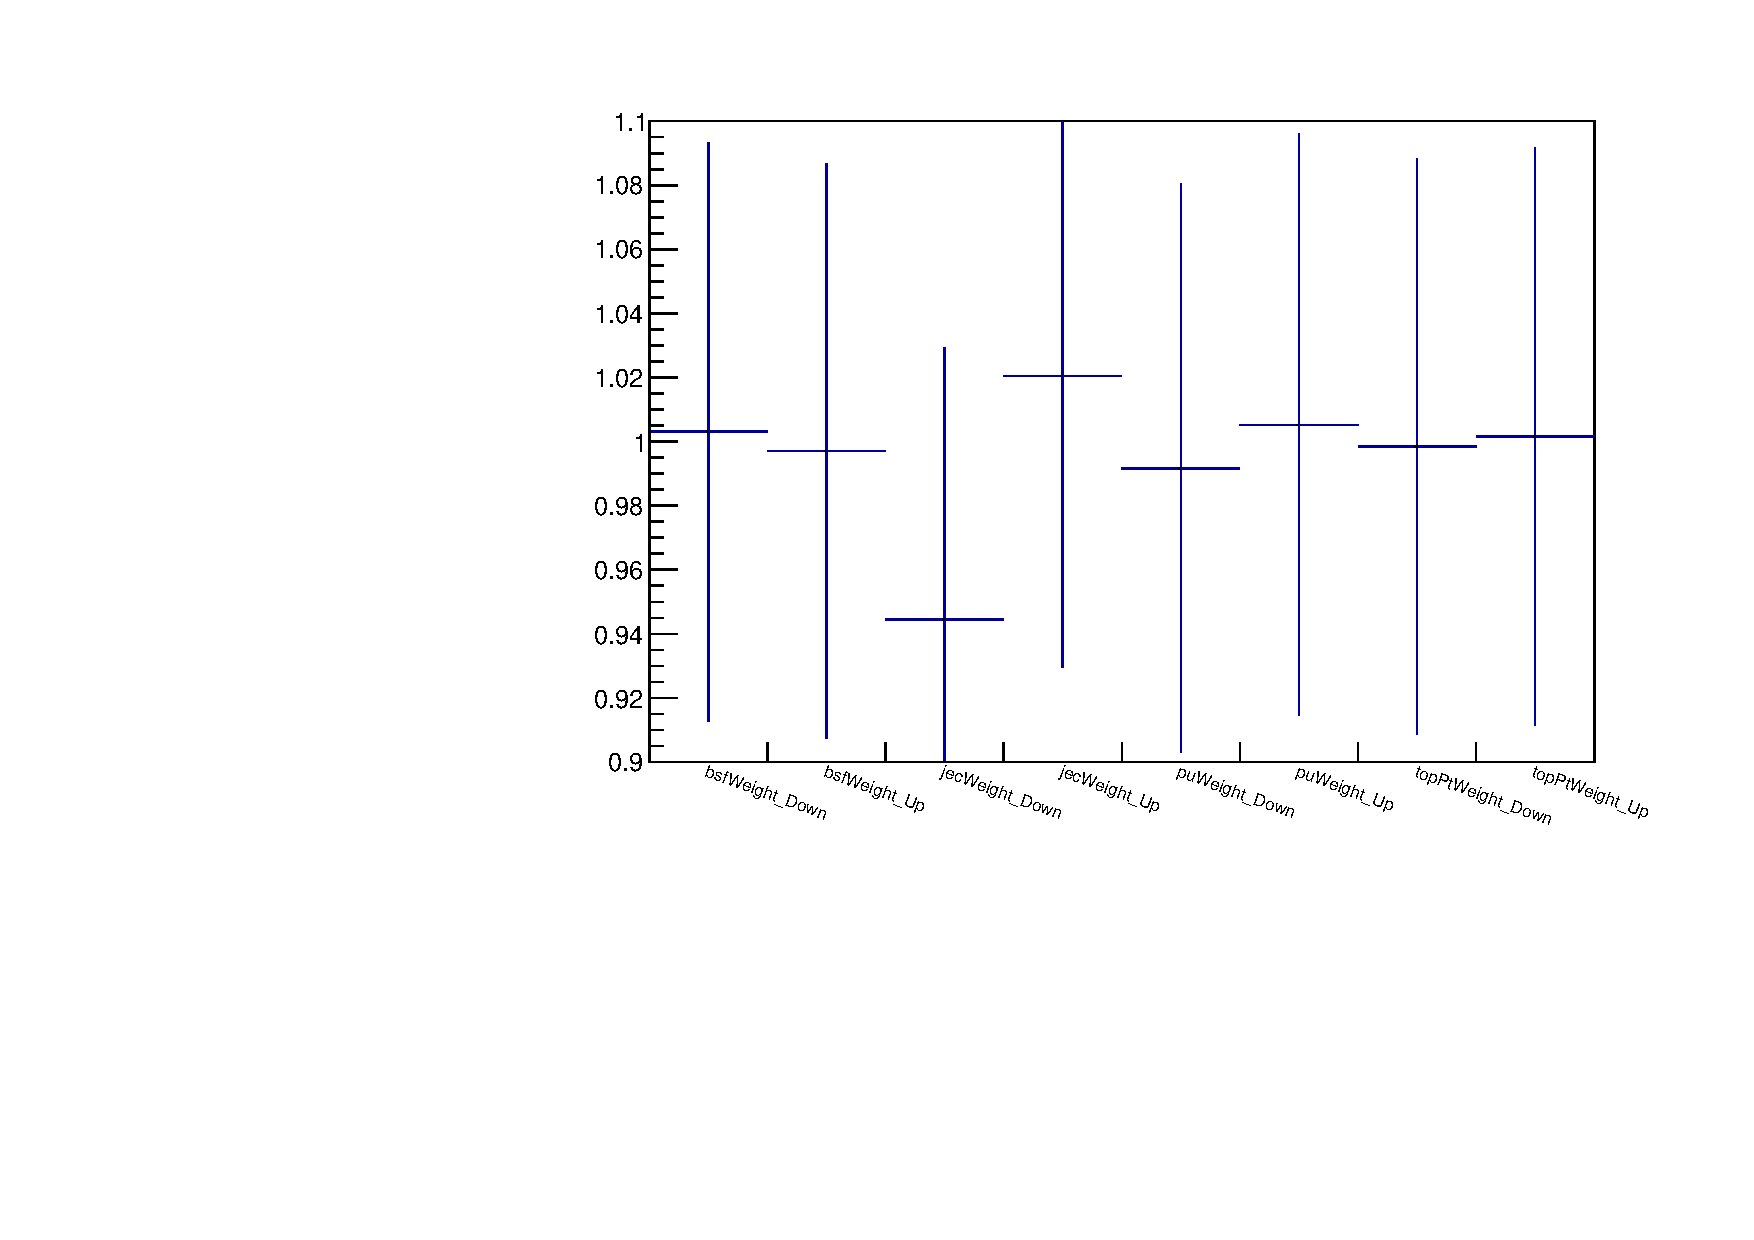
\includegraphics[width=0.9\textwidth]{figures/sideband_fit/summary_MhtSB_SinglePhoton.pdf}
  }~~
  \caption{Double ratio for \gj of change in MC yield under variations of known systematic sources in the sideband to the control region.
  The error bars represent the statistical uncertainty in the sideband and control region. No large biases (significantly higher than the statistical power of the sample) are observed.}
  \label{fig:pho-bias-sideband}
\end{figure}

\subsubsection{\mj and \mmj sideband}
For the $W$+jets, \ttbar+jets and $Z$+jets samples the cross section is know with better accuracy with respect to the \gj process, 
with NLO QCD or better precision.
However, some inconsinstency could arise from the different cross section calculations, since for \wj and \zj the LO cross sections 
are corrected with NLO k-factor (1.21 and 1.23 respectively) while for \ttbar the full NNLO calculation is used. \\
The corrections for these processes are derived using a sideband defined by inverting the \mht cut, namely 
applying the selection $100 < \mht < 130$ GeV. \\
As for the \gj sidebands, the change in the ratio of MC yields in the sideband
to the yields in the control region for several sources of systematic uncertainty is shown in 
Fig.~\ref{fig:mu-bias-sideband} and Fig.~\ref{fig:mumu-bias-sideband}. This again shows that any
bias in the sideband with respect to the control regions for these systematic sources is 
subdominant compared to the statistical uncertainty of the sample (shown in the error bars).
Any residual bias is accounted for by including these systematics 
in the fit when when deriving the sideband corrections.


\begin{figure}[!h]
  \centering
    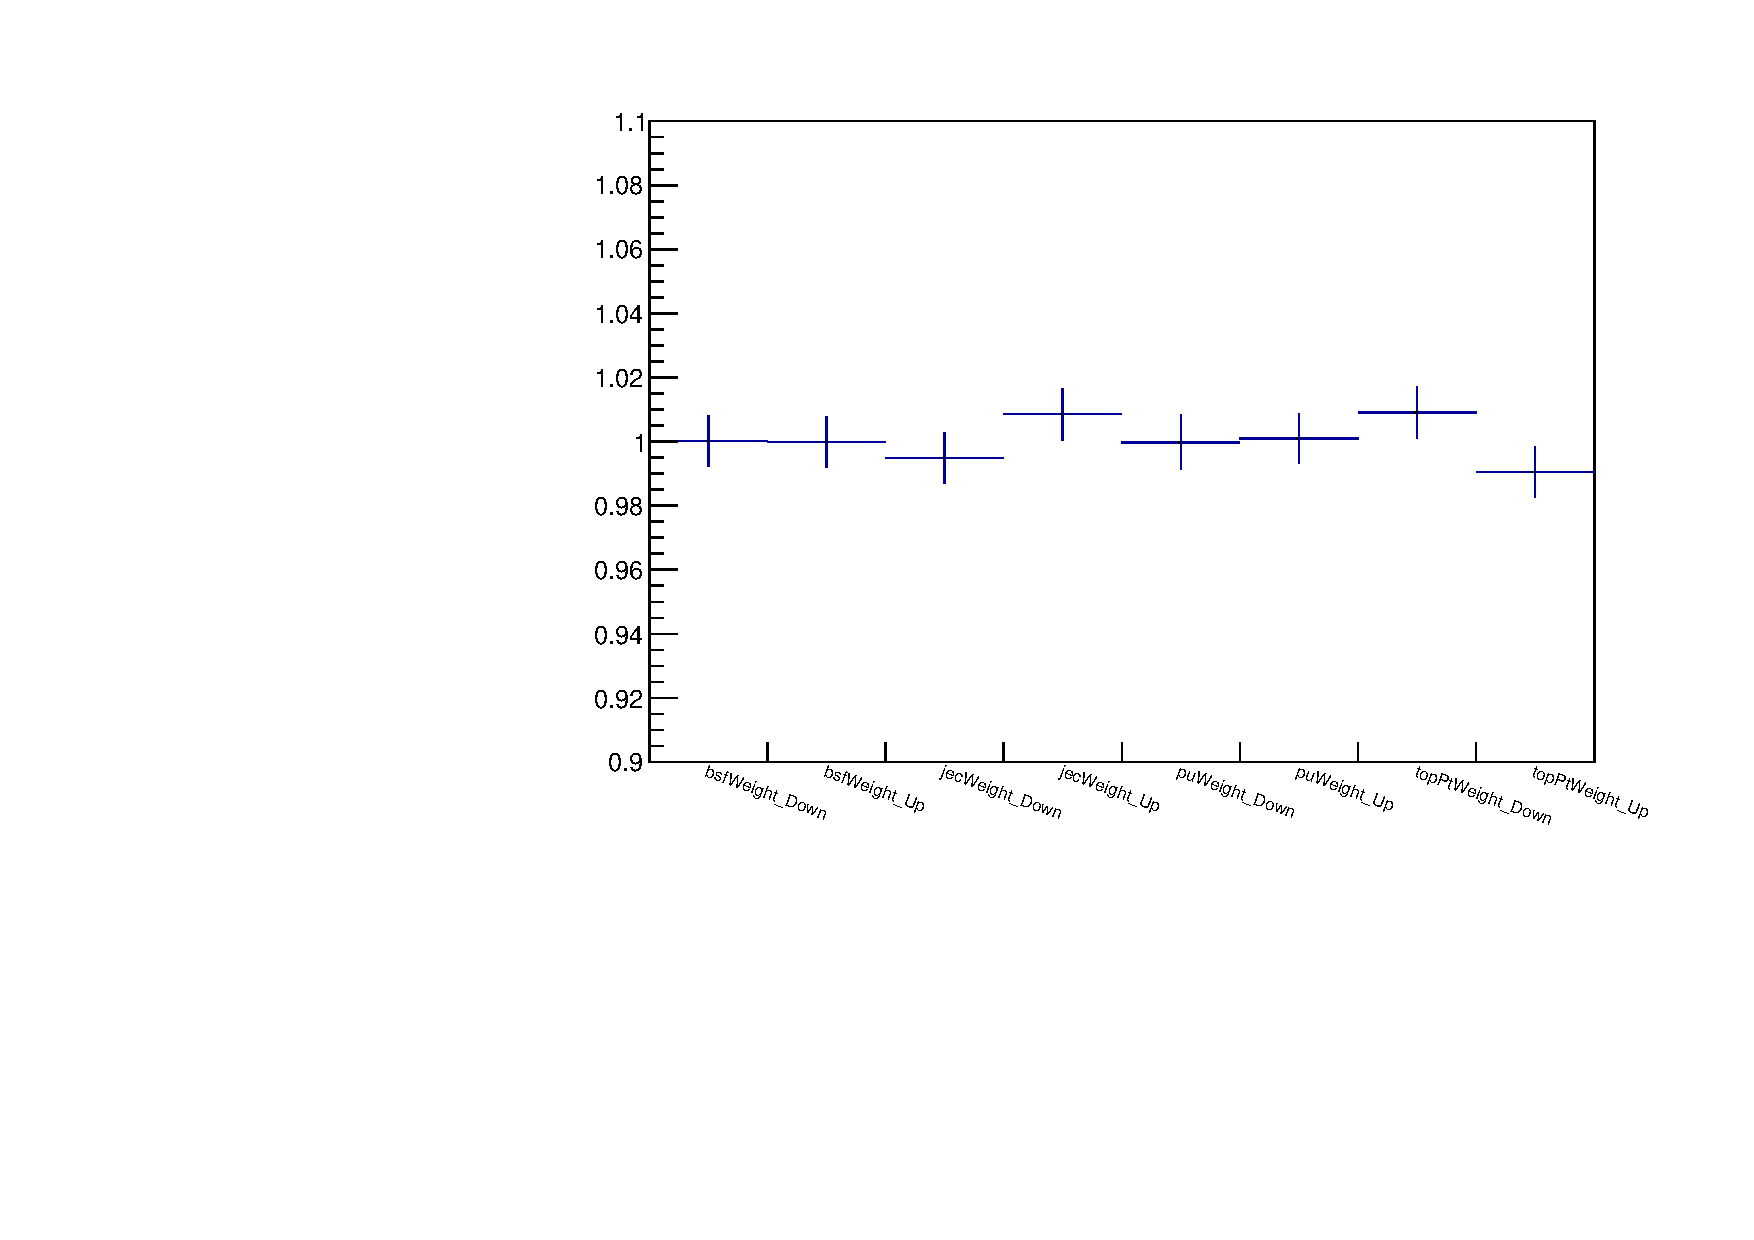
\includegraphics[width=0.9\textwidth]{figures/sideband_fit/summary_MhtSB_SingleMu.pdf}
  }~~
  \caption{Double ratio for \mj of change in MC yield under variations of known systematic sources in the sideband to the control region.
  The error bars represent the statistical uncertainty in the sideband and control region. No large biases (significantly higher than the statistical power of the sample) are observed.}
  \label{fig:mu-bias-sideband}
\end{figure}

\begin{figure}[!h]
  \centering
    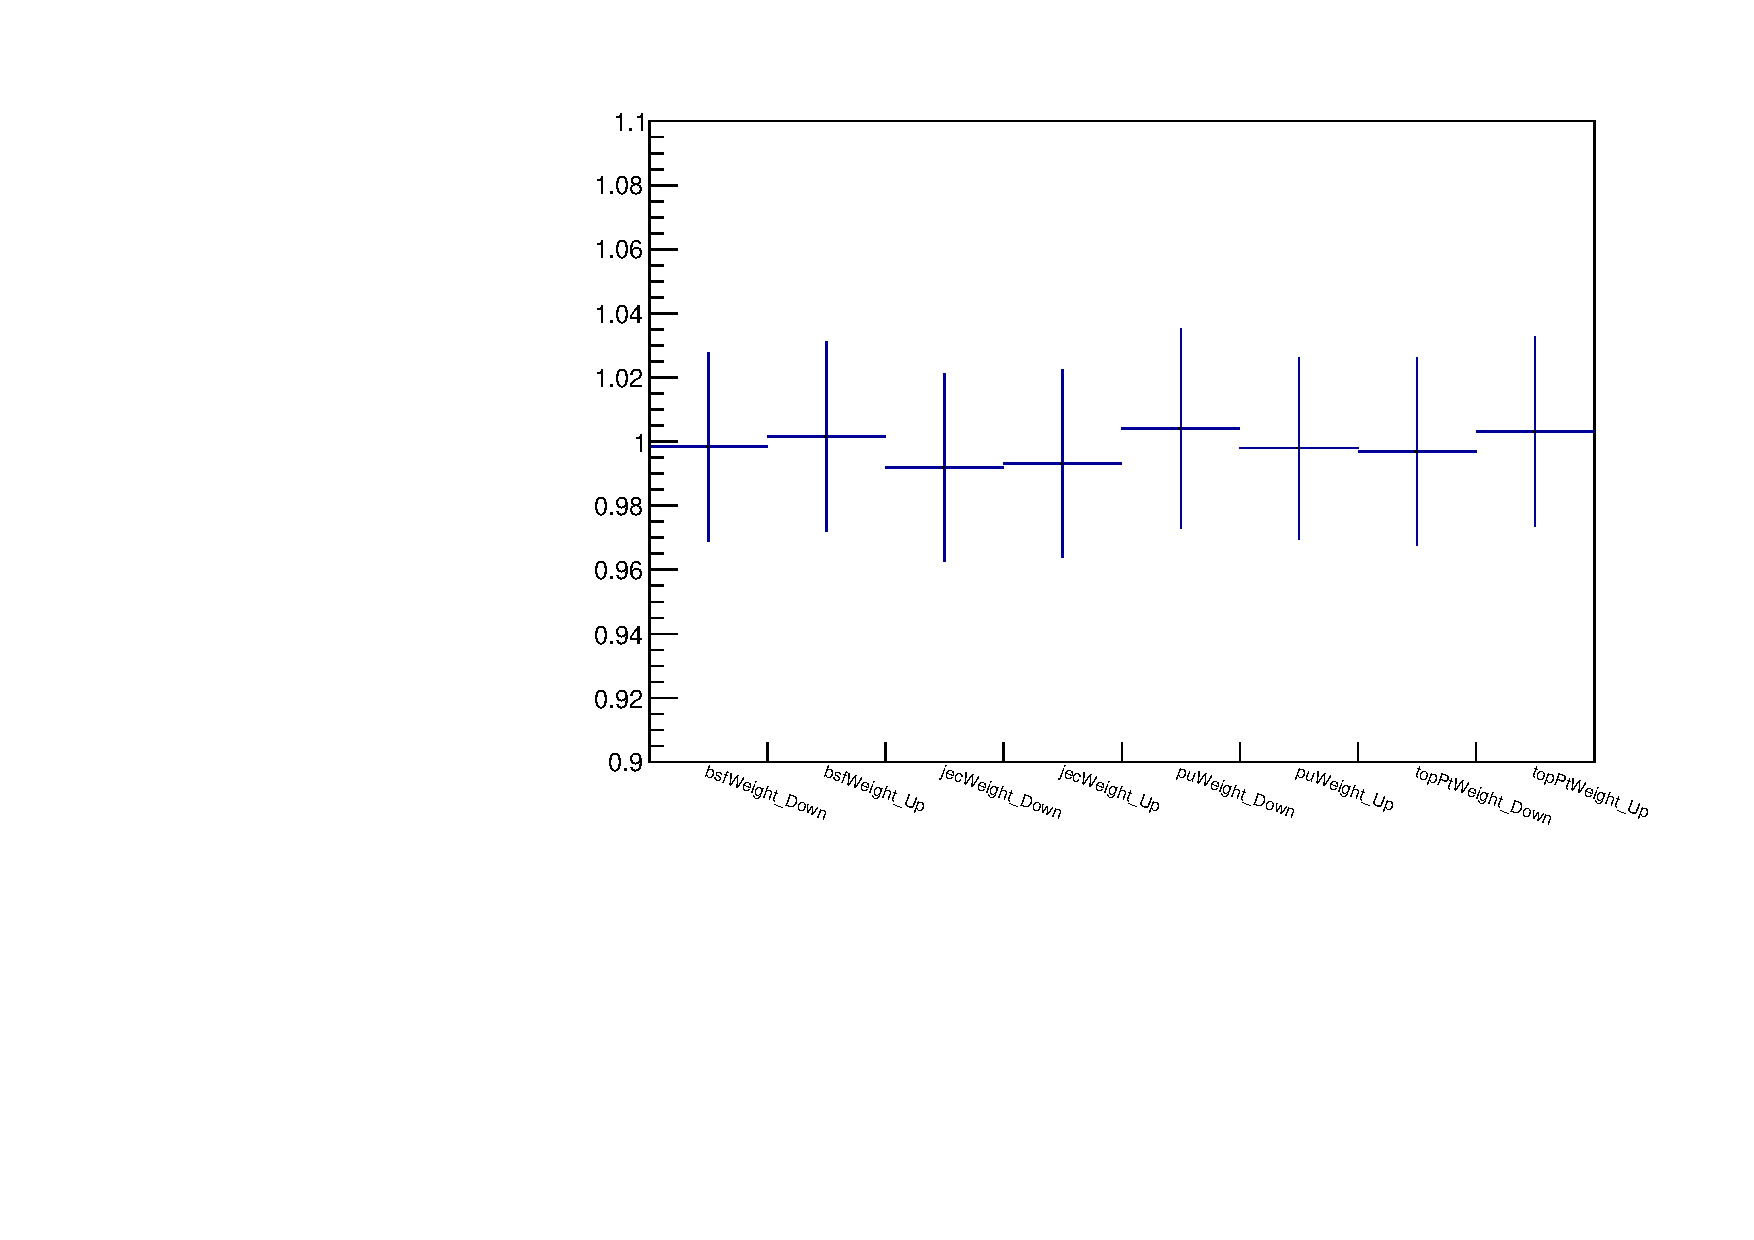
\includegraphics[width=0.9\textwidth]{figures/sideband_fit/summary_MhtSB_DoubleMu.pdf}
  }~~
  \caption{Double ratio for \mmj of change in MC yield under variations of known systematic sources in the sideband to the control region.
  The error bars represent the statistical uncertainty in the sideband and control region. No large biases (significantly higher than the statistical power of the sample) are observed.}
  \label{fig:mumu-bias-sideband}
\end{figure}
\subsection{Procedure for deriving sideband corrections}
\label{sec:fit-sideband}

To take advantage of the full phase space of the sidebands a simultaneous 
fit is used to derive the corrections for \wj, \zj, \ttbar and \gj. 
The sideband is binned identically to the control region in \njet, \nb and \scalht and a floating 
parameter per relevant process encodes the correction for that process (fully correlated across all bins).
The \wj and \ttbar processes are mainly constrained by the \mj sideband while the \zj and \gj processes are
wholey constrained by the \mmj and \gj sidebands respectively. The values of the corrections and uncertainties
given by the fit are shown in Table~\ref{tab:sbCorrsFromFit}.

\begin{table}[!h]
  \scriptsize
  \centering
  \topcaption{Cross section corrections for SM backgrounds derived with fit to sidebands in data.}
  \label{tab:sbCorrsFromFit}
  \begin{tabular}
    {cllc}
    \hline\hline
    \textbf{Process} & \textbf{Sideband} & \textbf{Selection} & \textbf{Corrrection} \\
    \hline
    \gj & $0.50 < \alphat < 0.52(0.53)$ & \gj & $1.43 \pm 0.07$ \\
    \wj & $100 < \mht < 130 \, \mathrm{GeV}$ & \mj& $1.23 \pm 0.02$ \\
    \zj & $100 < \mht < 130 \, \mathrm{GeV}$ & \mmj& $1.14 \pm 0.05$ \\
    \ttbar + jets & $100 < \mht < 130 \, \mathrm{GeV}$ & \mj, \mmj  & $0.9 \pm 0.02$ \\
    \hline \hline
  \end{tabular}
\end{table}

%% \section{Characterisation of the signal and control regions}
\label{sec:yields}

The event selection criteria for the signal and control regions are
detailed in Sec.~\ref{sec:selection}. A selection of relevant data/MC
comparison plots are presented here. The distributions are shown
separately according three \njet categories: symmetric, asymmetric,
and monojet. The distributions are intended to provide a qualitative
understanding of the simulation modelling for key variables. However, 
the analysis is not sensitive due to the reliance on simulation via
ratios only (\ie transfer factors) and the one-to-one mapping of
(\njet,~\nb,~\scalht) binning between the control and signal
regions. For monojet, the distributions of azimuthal angle of jets are 
included along with other key variables to demonstrate the absence of 
beam halo effects. The simulated distributions are normalized to an integrated
luminosity of 2.6~$\ifb$ (the data/MC scale factors are also shown
in all plots).

In addition to distributions, the binned yields in the \mj, \mmj, and
\gj control samples can be found in
Tables~\ref{tab:yieldssep_mu_data_sym}-\ref{tab:yieldssep_mu_data_mono},
\ref{tab:yieldssep_mumu_data_sym}-\ref{tab:yieldssep_mumu_data_mono},
and \ref{tab:yieldssep_gj_data_sym}-\ref{tab:yieldssep_gj_data_mono},
respectively, which correspond to an integrated luminosity of 2.6
\ifb. 
Finally, Tables~\ref{tab:yieldsnodata_sig_comb_sym},
\ref{tab:yieldsnodata_sig_comb_asym} and \ref{tab:yieldsnodata_sig_comb_mono} summarise the expected yields, as
determined from simulation, in the signal region for an integrated
luminosity of 2.6 \ifb.

\clearpage
\subsection{Yields and distributions for the $\mu$ + jets control sample}

\begin{table}[h!]
\tiny
\centering
\caption{Yields in the \mj control region for 2.1\ifb for symmetric categories.\label{tab:yieldssep_mu_data_sym}}
\scalebox{0.85}{\begin{tabular}{ccccccccc}
	\hline\hline
	& \multicolumn{8}{c}{\scalht (\gev)} \\ 
	 (\njet,  \nb) & 200-250 & 250-300 & 300-350 & 350-400 & 400-500 & 500-600 & 600-800 & 800-$\infty$ \\ [0.8ex] 
\hline
	(2, 0) & 451 & 660 & 611 & 491 & 615 & 285 & 226 & 116 \\[0.5ex] 
	(2, 1) & 74 & 68 & 57 & 54 & 80 & 49 & 28 & 13 \\[0.5ex] 
	(2, 2) & 2 & 2 & 5 & 1 & 6 & 5 & 2 & -- \\[0.5ex] 
	(3, 0) & 1 & 199 & 419 & 405 & 654 & 356 & 312 & 170 \\[0.5ex] 
	(3, 1) & -- & 86 & 164 & 186 & 235 & 105 & 95 & 31 \\[0.5ex] 
	(3, 2) & -- & 24 & 58 & 57 & 64 & 30 & 18 & 11 \\[0.5ex] 
	(3, $\ge3$) & -- & 1 & -- & -- & 3 & -- & -- & -- \\[0.5ex] 
	(4, 0) & -- & -- & 40 & 142 & 348 & 265 & 265 & 154 \\[0.5ex] 
	(4, 1) & -- & -- & 38 & 130 & 244 & 159 & 130 & 50 \\[0.5ex] 
	(4, 2) & -- & -- & 10 & 54 & 125 & 56 & 55 & 25 \\[0.5ex] 
	(4, $\ge3$) & -- & -- & 1 & 5 & 6 & 4 & 2 & 3 \\[0.5ex] 
	($\ge5$, 0) & -- & -- & -- & 16 & 99 & 132 & 183 & 144 \\[0.5ex] 
	($\ge5$, 1) & -- & -- & -- & 8 & 110 & 159 & 195 & 139 \\[0.5ex] 
	($\ge5$, 2) & -- & -- & -- & 6 & 57 & 90 & 109 & 69 \\[0.5ex] 
	($\ge5$, $\ge3$) & -- & -- & -- & -- & 2 & 6 & 14 & 12 \\[0.5ex] 
	\hline
	\hline
\end{tabular}}
\end{table}

\begin{table}[h!]
\tiny
\centering
\caption{Data in the \mj control region for 6.26\ifb for asymmetric categories.\label{tab:yieldssep_mu_data_asym}}
\scalebox{0.85}{\begin{tabular}{ccccccccc}
	\hline\hline
	& \multicolumn{8}{c}{\scalht (\gev)} \\ 
	 (\njet,  \nb) & 200-250 & 250-300 & 300-350 & 350-400 & 400-500 & 500-600 & 600-800 & 800-$\infty$ \\ [0.8ex] 
\hline
	(2a, 0) & 12940 & 6805 & 3203 & 1389 & 941 & 242 & 104 & -- \\[0.5ex] 
	(2a, 1) & 2209 & 968 & 431 & 199 & 128 & 29 & -- & -- \\[0.5ex] 
	(2a, 2) & 182 & 84 & 42 & 7 & 8 & -- & -- & -- \\[0.5ex] 
	(3a, 0) & 2846 & 3814 & 2173 & 1104 & 766 & 176 & 60 & -- \\[0.5ex] 
	(3a, 1) & 1524 & 1790 & 912 & 377 & 221 & 37 & 27 & -- \\[0.5ex] 
	(3a, 2) & 419 & 551 & 268 & 96 & 57 & 16 & -- & -- \\[0.5ex] 
	(3a, $\ge3$) & 10 & 24 & 7 & -- & -- & -- & -- & -- \\[0.5ex] 
	(4a, 0) & 26 & 521 & 850 & 544 & 467 & 123 & 39 & -- \\[0.5ex] 
	(4a, 1) & 26 & 457 & 761 & 488 & 332 & 74 & 20 & -- \\[0.5ex] 
	(4a, 2) & 9 & 201 & 382 & 230 & 147 & 29 & 10 & -- \\[0.5ex] 
	(4a, $\ge3$) & -- & 12 & 21 & 23 & 7 & -- & -- & -- \\[0.5ex] 
	($\ge5$a, 0) & -- & 1 & 68 & 171 & 280 & 100 & 30 & -- \\[0.5ex] 
	($\ge5$a, 1) & -- & 3 & 98 & 194 & 306 & 96 & 45 & -- \\[0.5ex] 
	($\ge5$a, 2) & -- & 3 & 46 & 128 & 203 & 66 & 18 & -- \\[0.5ex] 
	($\ge5$a, $\ge3$) & -- & -- & 6 & 15 & 30 & 8 & -- & -- \\[0.5ex] 
	\hline
	\hline
\end{tabular}}
\end{table}

\begin{table}[h!]
\tiny
\centering
\caption{Yields in the \mj control region for 2.1\ifb for monojet categories.\label{tab:yieldssep_mu_data_mono}}
\begin{tabular}
{ccccccccc}
	\hline\hline
	& \multicolumn{8}{c}{\scalht (\gev)} \\ 
	 (\njet,  \nb) & 200-250 & 250-300 & 300-350 & 350-400 & 400-500 & 500-600 & 600-800 & 800-$\infty$ \\ [0.8ex] 
\hline
	(1, 0) & 4022 & 1498 & 597 & 282 & 246 & 81 & 34 & -- \\[0.5ex] 
	(1, 1) & 196 & 65 & 21 & 14 & 12 & 1 & -- & -- \\[0.5ex] 
	\hline
	\hline
\end{tabular}
\end{table}


\clearpage
\begin{figure}
    \begin{center}
        \subfigure {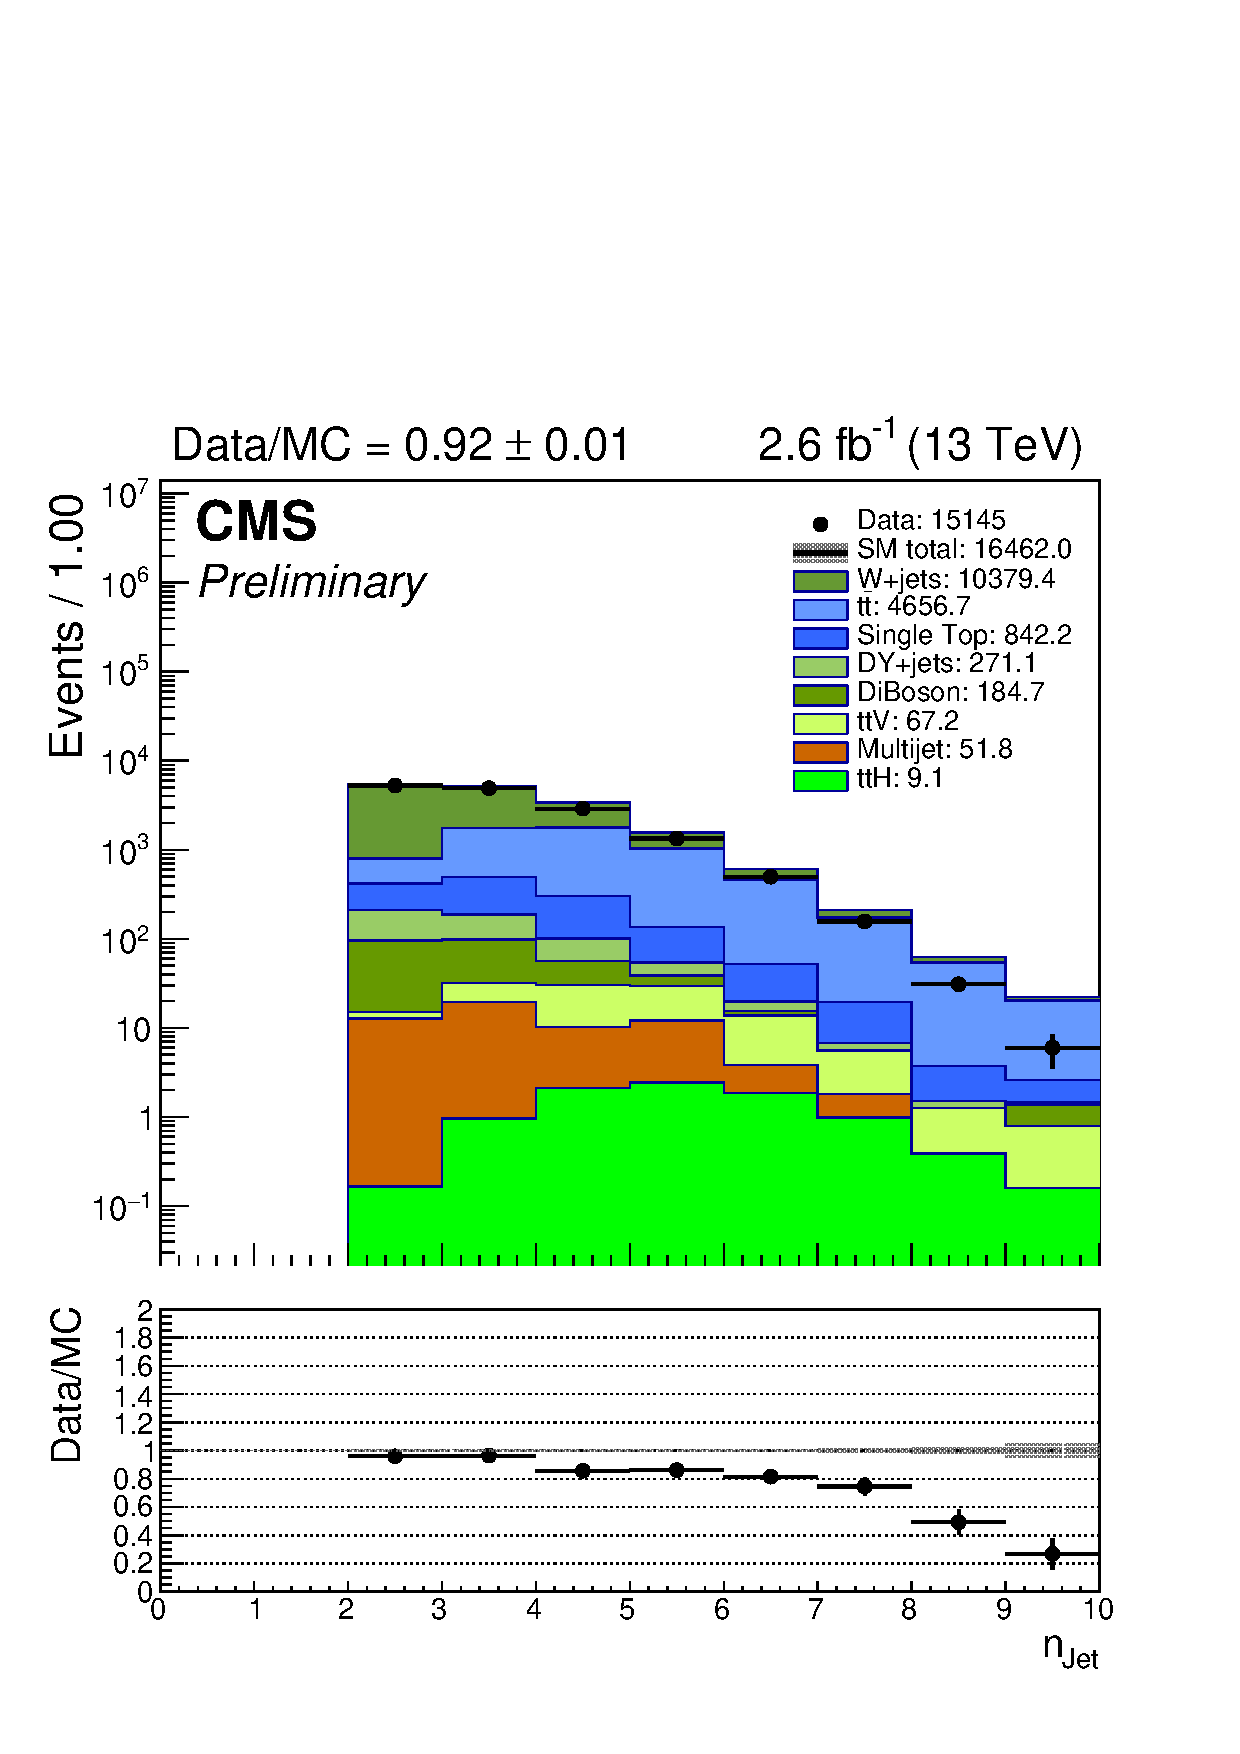
\includegraphics[width=0.5\textwidth]{figures/distributions/SingleMu/nJet40_sym.pdf}} ~~
        \subfigure {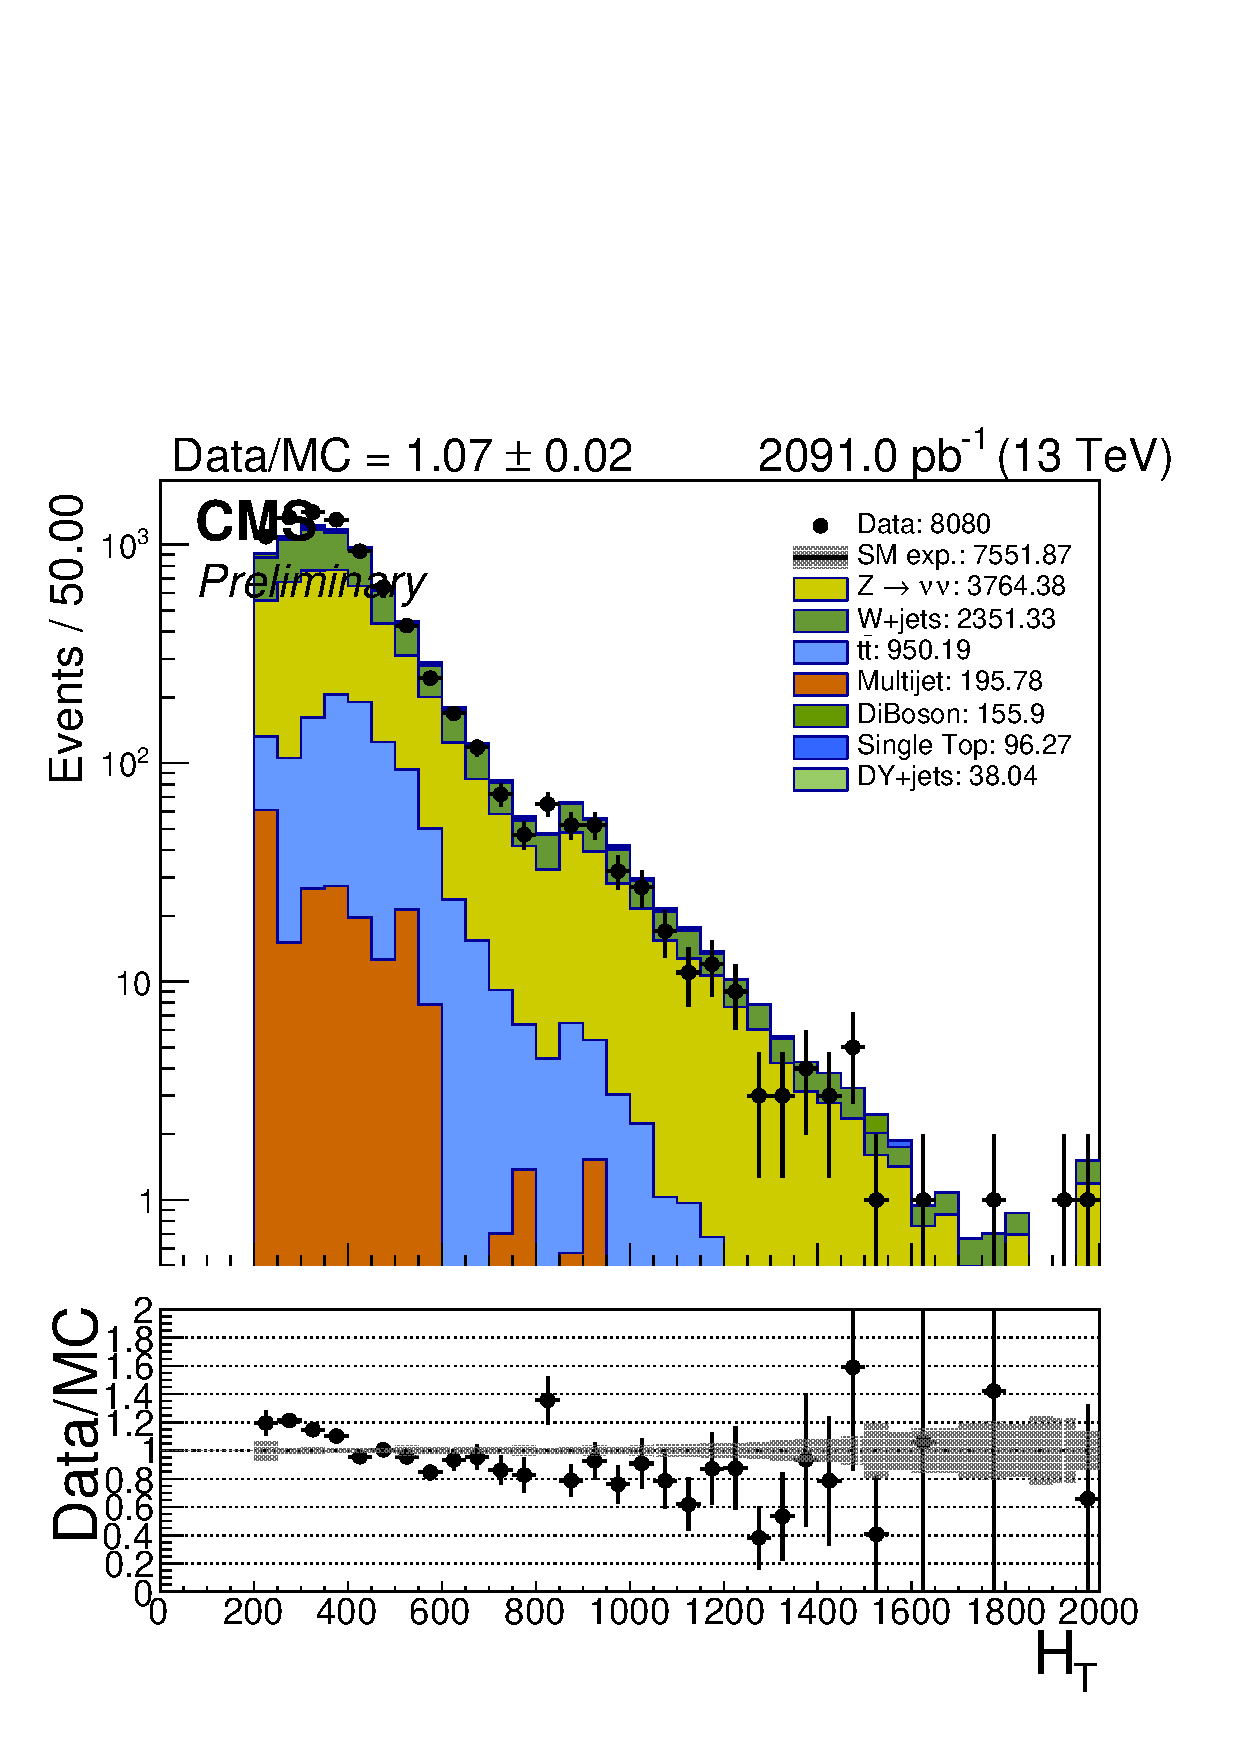
\includegraphics[width=0.5\textwidth]{figures/distributions/SingleMu/ht40_sym.pdf}} \\
        \subfigure {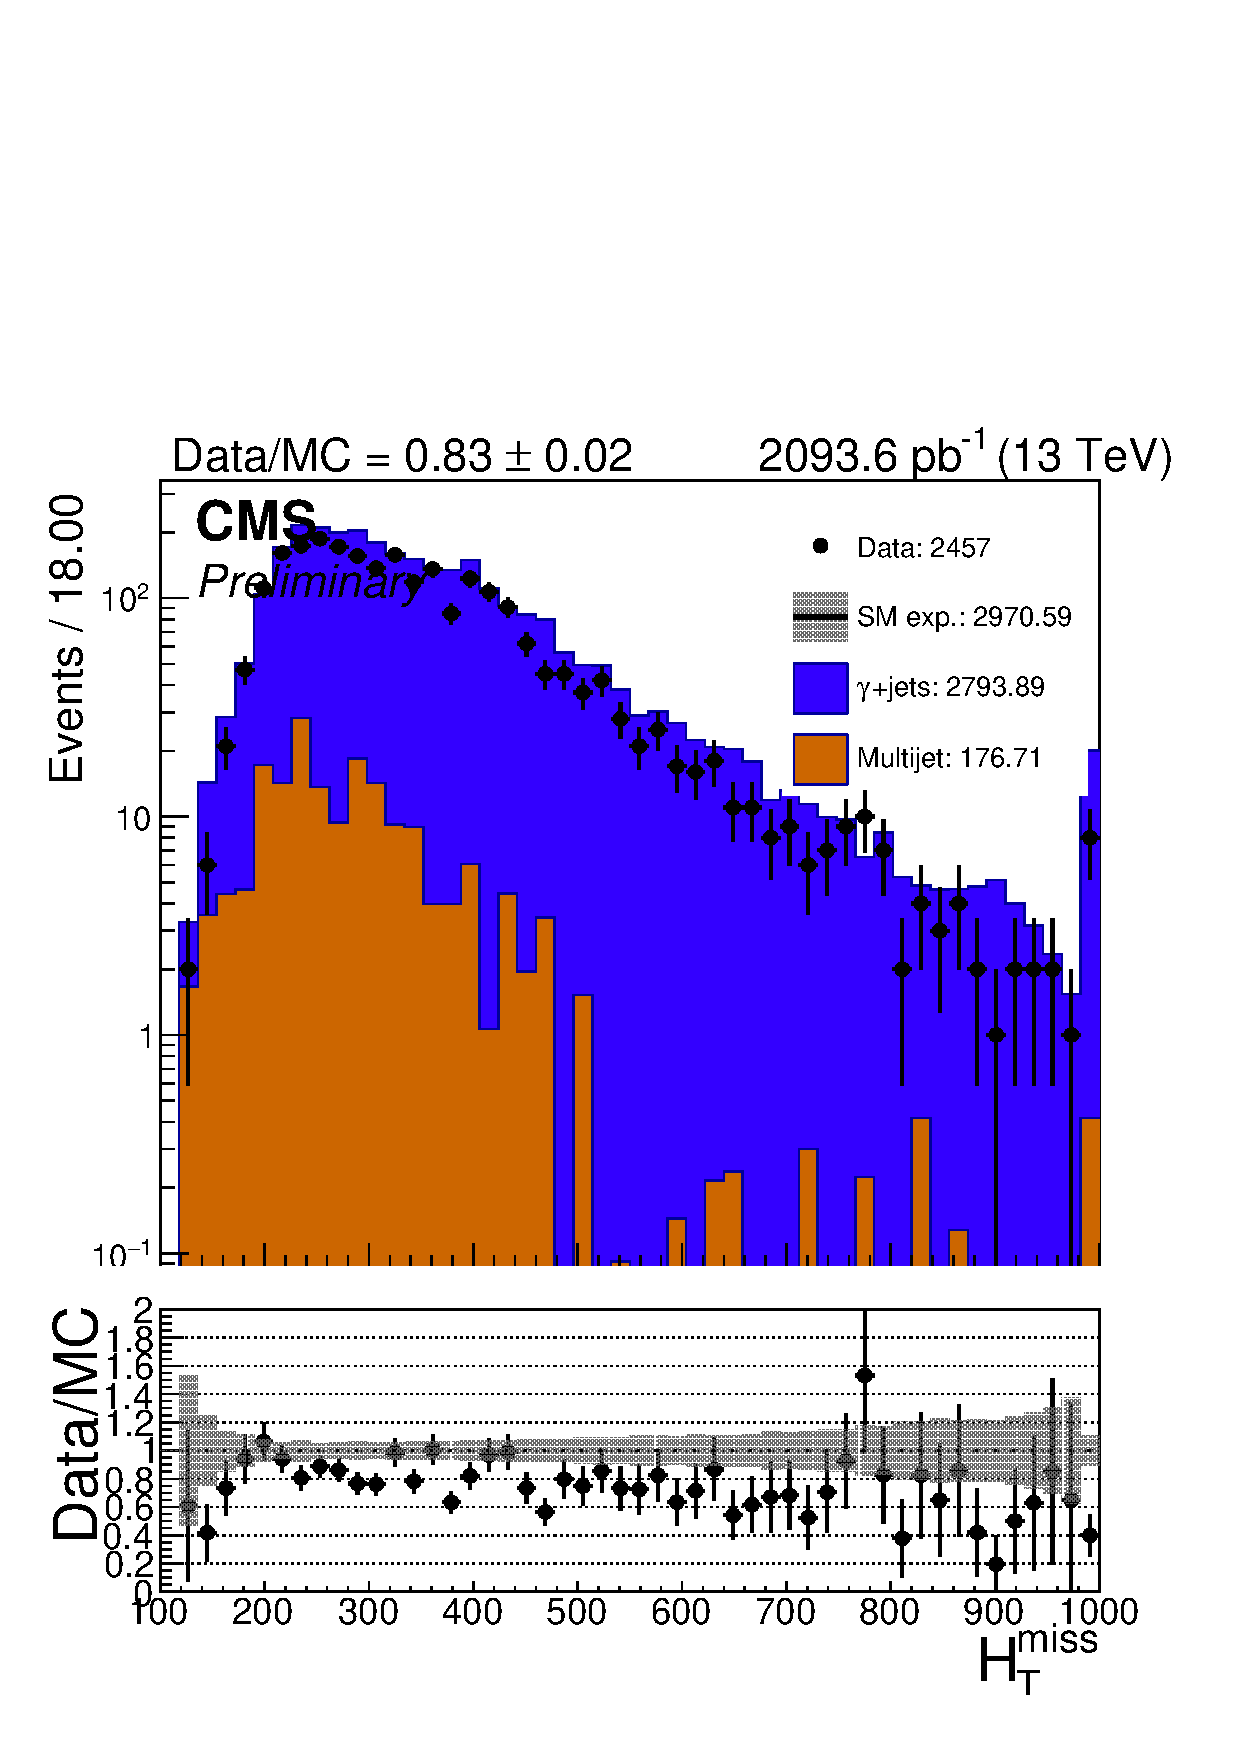
\includegraphics[width=0.5\textwidth]{figures/distributions/SingleMu/mht40_pt_sym.pdf}} ~~
        \subfigure {\includegraphics[width=0.5\textwidth]{figures/distributions/SingleMu/nBJet40_sym.pdf}} \\
        \caption{Key analysis variables for single muon control region (symmetric \njet bins)}
        \label{fig:distribution_singlemu_sym}
    \end{center}
\end{figure}

\clearpage
\begin{figure}
    \begin{center}
        \subfigure {\includegraphics[width=0.5\textwidth]{figures/distributions/SingleMu/nJet40_asym.pdf}} ~~
        \subfigure {\includegraphics[width=0.5\textwidth]{figures/distributions/SingleMu/ht40_asym.pdf}} \\
        \subfigure {\includegraphics[width=0.5\textwidth]{figures/distributions/SingleMu/mht40_pt_asym.pdf}} ~~
        \subfigure {\includegraphics[width=0.5\textwidth]{figures/distributions/SingleMu/nBJet40_asym.pdf}} \\
        \caption{Key analysis variables for single muon control region (asymmetric \njet bins)}
        \label{fig:distribution_singlemu_asym}
    \end{center}
\end{figure}

\clearpage
\begin{figure}
    \begin{center}        
        \subfigure {\includegraphics[width=0.5\textwidth]{figures/distributions/SingleMu/jet_pt[0]_eq1j.pdf}} ~~
        \subfigure {\includegraphics[width=0.5\textwidth]{figures/distributions/SingleMu/njetInc_eq1j.pdf}} \\
        \subfigure {\includegraphics[width=0.5\textwidth]{figures/distributions/SingleMu/nBJet40_eq1j.pdf}} ~~
        \subfigure {\includegraphics[width=0.5\textwidth]{figures/distributions/SingleMu/jet_phi[0]_eq1j.pdf}} \\
        \caption{Key analysis variables for single muon control region (monojet bins)}
        \label{fig:distribution_singlemu_mono}
    \end{center}
\end{figure}

\clearpage
\subsection{Yields and distributions for the $\mu\mu$ + jets control sample}

\begin{table}[h!]
\tiny
\centering
\topcaption{Yields in the \mmj control region for 1.26\ifb for symmetric categories. The letter ``a'' in jet \eg ``2a''  indicates the asymmetric jet bins. All entries are non-zero but are truncated to one decimal place.\label{tab:yieldssep_data_mumu_sym}}
\begin{tabular}
{ccccccccc}
	\hline\hline
&	& \multicolumn{8}{c}{\scalht (\gev)} \\ 
	 (\njet,  \nb) & 200-250 & 250-300 & 300-350 & 350-400 & 400-500 & 500-600 & 600-800 & 800-$\infty$ \\ [0.8ex] 
\hline
	(2, 0) & 37 & 45 & 41 & 23 & 33 & 25 & 12 & 6 \\[0.5ex] 
	(2, 1) & 3 & 5 & 8 & 2 & 5 & 1 & 1 & 1 \\[0.5ex] 
	(2, 2) & 0 & 0 & 0 & -- & 0 & 0 & 0 & 0 \\[0.5ex] 
	(3, 0) & 0 & 8 & 25 & 27 & 30 & 23 & 10 & 10 \\[0.5ex] 
	(3, 1) & 0 & 2 & 3 & 4 & 1 & 1 & 4 & 2 \\[0.5ex] 
	(3, 2) & -- & 1 & 2 & 0 & 0 & 0 & 1 & 0 \\[0.5ex] 
	(3, $\ge3$) & -- & -- & -- & 0 & 0 & 0 & -- & -- \\[0.5ex] 
	(4, 0) & -- & -- & 3 & 1 & 13 & 11 & 16 & 10 \\[0.5ex] 
	(4, 1) & -- & -- & 1 & 1 & 2 & 0 & 3 & 4 \\[0.5ex] 
	(4, 2) & -- & -- & 0 & 0 & 0 & 0 & 0 & 1 \\[0.5ex] 
	(4, $\ge3$) & -- & -- & -- & 0 & 0 & 0 & 0 & 0 \\[0.5ex] 
	($\ge5$, 0) & -- & -- & -- & 0 & 2 & 4 & 5 & 10 \\[0.5ex] 
	($\ge5$, 1) & -- & -- & -- & 0 & 1 & 4 & 2 & 2 \\[0.5ex] 
	($\ge5$, 2) & -- & -- & -- & 0 & 0 & 0 & 1 & 2 \\[0.5ex] 
	($\ge5$, $\ge3$) & -- & -- & -- & -- & 1 & 0 & 0 & 0 \\[0.5ex] 
	\hline
	\hline
\end{tabular}
\end{table}

\begin{table}[h!]
\tiny
\centering
\caption{Data in the \mmj control region for 12.9\ifb for asymmetric categories.\label{tab:yieldssep_mumu_data_asym}}
\scalebox{0.85}{\begin{tabular}{ccccccccc}
	\hline\hline
	& \multicolumn{8}{c}{\scalht (\gev)} \\ 
	 (\njet,  \nb) & 200-250 & 250-300 & 300-350 & 350-400 & 400-500 & 500-600 & 600-800 & 800-$\infty$ \\ [0.8ex] 
\hline
	(2a, 0) & 2405 & 1362 & 691 & 295 & 239 & 60 & 20 & -- \\[0.5ex] 
	(2a, 1) & 289 & 144 & 78 & 31 & 20 & 7 & -- & -- \\[0.5ex] 
	(2a, 2) & 36 & 19 & 11 & 3 & 0 & -- & -- & -- \\[0.5ex] 
	(3a, 0) & 434 & 600 & 352 & 199 & 157 & 39 & 11 & -- \\[0.5ex] 
	(3a, 1) & 67 & 98 & 78 & 24 & 28 & 14 & 0 & -- \\[0.5ex] 
	(3a, 2) & 15 & 14 & 15 & 10 & 4 & 0 & -- & -- \\[0.5ex] 
	(3a, $\ge3$) & 0 & 0 & 0 & -- & -- & -- & -- & -- \\[0.5ex] 
	(4a, 0) & 2 & 57 & 105 & 69 & 67 & 14 & 3 & -- \\[0.5ex] 
	(4a, 1) & 2 & 16 & 31 & 21 & 16 & 3 & 1 & -- \\[0.5ex] 
	(4a, 2) & 0 & 5 & 15 & 4 & 3 & 0 & 0 & -- \\[0.5ex] 
	(4a, $\ge3$) & -- & 0 & 1 & 0 & 1 & -- & -- & -- \\[0.5ex] 
	($\ge5$a, 0) & -- & 0 & 6 & 17 & 26 & 14 & 6 & -- \\[0.5ex] 
	($\ge5$a, 1) & -- & 0 & 3 & 3 & 15 & 3 & 0 & -- \\[0.5ex] 
	($\ge5$a, 2) & -- & 1 & 1 & 4 & 2 & 1 & 0 & -- \\[0.5ex] 
	($\ge5$a, $\ge3$) & -- & -- & 0 & 1 & 1 & 0 & -- & -- \\[0.5ex] 
	\hline
	\hline
\end{tabular}}
\end{table}

\begin{table}[h!]
\tiny
\centering
\caption{Data in the \mmj control region for 2.2\ifb for monojet categories.\label{tab:yieldssep_mumu_data_mono}}
\scalebox{0.85}{\begin{tabular}{ccccccccc}
	\hline\hline
	& \multicolumn{8}{c}{\scalht (\gev)} \\ 
	 (\njet,  \nb) & 200-250 & 250-300 & 300-350 & 350-400 & 400-500 & 500-600 & 600-800 & 800-$\infty$ \\ [0.8ex] 
\hline
	(1, 0) & 518 & 193 & 99 & 37 & 31 & 14 & 6 & -- \\[0.5ex] 
	(1, 1) & 18 & 13 & 6 & 0 & 1 & 1 & -- & -- \\[0.5ex] 
	\hline
	\hline
\end{tabular}}
\end{table}


\clearpage
\begin{figure}
    \begin{center}
        \subfigure {\includegraphics[width=0.5\textwidth]{figures/distributions/DoubleMu/nJet40_sym.pdf}} ~~
        \subfigure {\includegraphics[width=0.5\textwidth]{figures/distributions/DoubleMu/ht40_sym.pdf}} \\
        \subfigure {\includegraphics[width=0.5\textwidth]{figures/distributions/DoubleMu/mht40_pt_sym.pdf}} ~~
        \subfigure {\includegraphics[width=0.5\textwidth]{figures/distributions/DoubleMu/nBJet40_sym.pdf}} \\
        \caption{Key analysis variables for double muon control region (symmetric \njet bins)}
        \label{fig:distribution_doublemu_sym}
    \end{center}
\end{figure}

\clearpage
\begin{figure}
    \begin{center}
        \subfigure {\includegraphics[width=0.5\textwidth]{figures/distributions/DoubleMu/nJet40_asym.pdf}} ~~
        \subfigure {\includegraphics[width=0.5\textwidth]{figures/distributions/DoubleMu/ht40_asym.pdf}} \\
        \subfigure {\includegraphics[width=0.5\textwidth]{figures/distributions/DoubleMu/mht40_pt_asym.pdf}} ~~
        \subfigure {\includegraphics[width=0.5\textwidth]{figures/distributions/DoubleMu/nBJet40_asym.pdf}} \\
        \caption{Key analysis variables for double muon control region (asymmetric \njet bins)}
        \label{fig:distribution_doublemu_asym}
    \end{center}
\end{figure}

\begin{figure}
    \begin{center} 
        \subfigure {\includegraphics[width=0.5\textwidth]{figures/distributions/DoubleMu/jet_pt[0]_eq1j.pdf}} ~~
        \subfigure {\includegraphics[width=0.5\textwidth]{figures/distributions/DoubleMu/njetInc_eq1j.pdf}} \\
        \subfigure {\includegraphics[width=0.5\textwidth]{figures/distributions/DoubleMu/nBJet40_eq1j.pdf}} ~~
        \subfigure {\includegraphics[width=0.5\textwidth]{figures/distributions/DoubleMu/jet_phi[0]_eq1j.pdf}} \\
        \caption{Key analysis variables for double muon control region (monojet bins)}
        \label{fig:distribution_doublemu_mono}
    \end{center}
\end{figure}

\clearpage
\subsection{Yields and distributions for the photon + jets control sample}

\begin{table}[h!]
\tiny
\centering
\caption{Yields in the \gj control region for 1.26\ifb for symmetric categories. The letter ``a'' in jet \eg ``2a''  indicates the asymmetric jet bins. All entries are non-zero but are truncated to one decimal place.\label{tab:yieldssep_data_gj_sym}}
\begin{tabular}
{ccccc}
	\hline\hline
&	& \multicolumn{4}{c}{\scalht (\gev)} \\ 
	 (\njet,  \nb) & 400-500 & 500-600 & 600-800 & 800-$\infty$ \\ [0.8ex] 
\hline
	(2, 0) & 189 & 65 & 37 & 76 \\[0.5ex] 
	(2, 1) & 9 & 1 & 0 & 7 \\[0.5ex] 
	(2, 2) & 0 & 0 & 0 & 0 \\[0.5ex] 
	(3, 0) & 272 & 122 & 69 & 132 \\[0.5ex] 
	(3, 1) & 23 & 13 & 8 & 24 \\[0.5ex] 
	(3, 2) & 4 & 0 & 2 & 1 \\[0.5ex] 
	(3, $\ge3$) & 1 & 0 & -- & -- \\[0.5ex] 
	(4, 0) & 132 & 92 & 73 & 83 \\[0.5ex] 
	(4, 1) & 20 & 16 & 6 & 22 \\[0.5ex] 
	(4, 2) & 2 & 1 & 1 & 2 \\[0.5ex] 
	(4, $\ge3$) & 0 & 0 & 1 & 0 \\[0.5ex] 
	($\ge5$, 0) & 26 & 40 & 49 & 63 \\[0.5ex] 
	($\ge5$, 1) & 3 & 5 & 9 & 15 \\[0.5ex] 
	($\ge5$, 2) & 2 & 3 & 1 & 4 \\[0.5ex] 
	($\ge5$, $\ge3$) & 0 & 0 & 0 & 0 \\[0.5ex] 
	\hline
	\hline
\end{tabular}
\end{table}

\begin{table}[h!]
\tiny
\centering
\caption{Data in the \gj control region for 2.2\ifb for asymmetric categories.\label{tab:yieldssep_gj_data_asym}}
\scalebox{0.85}{\begin{tabular}{ccccc}
	\hline\hline
	& \multicolumn{4}{c}{\scalht (\gev)} \\ 
	 (\njet,  \nb) & 400-500 & 500-600 & 600-800 & 800-$\infty$ \\ [0.8ex] 
\hline
	(2a, 0) & 164 & 44 & 17 & -- \\[0.5ex] 
	(2a, 1) & 16 & 2 & -- & -- \\[0.5ex] 
	(2a, 2) & 1 & -- & -- & -- \\[0.5ex] 
	(3a, 0) & 105 & 17 & 8 & -- \\[0.5ex] 
	(3a, 1) & 7 & 2 & 2 & -- \\[0.5ex] 
	(3a, 2) & 1 & 0 & -- & -- \\[0.5ex] 
	(3a, $\ge3$) & -- & -- & -- & -- \\[0.5ex] 
	(4a, 0) & 112 & 13 & 3 & -- \\[0.5ex] 
	(4a, 1) & 16 & 5 & 0 & -- \\[0.5ex] 
	(4a, 2) & 1 & 0 & 0 & -- \\[0.5ex] 
	(4a, $\ge3$) & 0 & -- & -- & -- \\[0.5ex] 
	($\ge5$a, 0) & 55 & 12 & 4 & -- \\[0.5ex] 
	($\ge5$a, 1) & 10 & 6 & 0 & -- \\[0.5ex] 
	($\ge5$a, 2) & 3 & 0 & 0 & -- \\[0.5ex] 
	($\ge5$a, $\ge3$) & 0 & 0 & -- & -- \\[0.5ex] 
	\hline
	\hline
\end{tabular}}
\end{table}

\begin{table}[h!]
\tiny
\centering
\caption{Data in the \gj control region for 2.1\ifb for monojet categories.\label{tab:yieldssep_gj_data_mono}}
\scalebox{0.85}{\begin{tabular}{ccccc}
	\hline\hline
	& \multicolumn{4}{c}{\scalht (\gev)} \\ 
	 (\njet,  \nb) & 400-500 & 500-600 & 600-800 & 800-$\infty$ \\ [0.8ex] 
\hline
	(1, 0) & 565 & 181 & 69 & -- \\[0.5ex] 
	(1, 1) & 23 & 6 & -- & -- \\[0.5ex] 
	\hline
	\hline
\end{tabular}}
\end{table}


\clearpage
\begin{figure}
    \begin{center}
        \subfigure {\includegraphics[width=0.5\textwidth]{figures/distributions/SinglePhoton/nJet40_sym.pdf}} ~~
        \subfigure {\includegraphics[width=0.5\textwidth]{figures/distributions/SinglePhoton/ht40_sym.pdf}} \\
        \subfigure {\includegraphics[width=0.5\textwidth]{figures/distributions/SinglePhoton/mht40_pt_sym.pdf}} ~~
        \subfigure {\includegraphics[width=0.5\textwidth]{figures/distributions/SinglePhoton/nBJet40_sym.pdf}} \\
        \caption{Key analysis variables for single photon control region (symmetric \njet bins)}
        \label{fig:distribution_singlephoton_sym}
    \end{center}
\end{figure}

\clearpage
\begin{figure}[h]
    \begin{center}
        \subfigure {\includegraphics[width=0.5\textwidth]{figures/distributions/SinglePhoton/nJet40_asym.pdf}} ~~
        \subfigure {\includegraphics[width=0.5\textwidth]{figures/distributions/SinglePhoton/ht40_asym.pdf}} \\
        \subfigure {\includegraphics[width=0.5\textwidth]{figures/distributions/SinglePhoton/mht40_pt_asym.pdf}} ~~
        \subfigure {\includegraphics[width=0.5\textwidth]{figures/distributions/SinglePhoton/nBJet40_asym.pdf}} \\
        \caption{Key analysis variables for single photon control region (asymmetric \njet bins)}
        \label{fig:distribution_singlephoton_asym}
    \end{center}
\end{figure}

\clearpage
\begin{figure}
    \begin{center} 
        \subfigure {\includegraphics[width=0.5\textwidth]{figures/distributions/SinglePhoton/jet_pt[0]_eq1j.pdf}} ~~
        \subfigure {\includegraphics[width=0.5\textwidth]{figures/distributions/SinglePhoton/njetInc_eq1j.pdf}} \\
        \subfigure {\includegraphics[width=0.5\textwidth]{figures/distributions/SinglePhoton/nBJet40_eq1j.pdf}} ~~
        \subfigure {\includegraphics[width=0.5\textwidth]{figures/distributions/SinglePhoton/jet_phi[0]_eq1j.pdf}} \\
        \caption{Key analysis variables for single photon control region (monojet bins)}
        \label{fig:distribution_singlephoton_mono}
    \end{center}
\end{figure}

\clearpage
\subsection{Expected yields and distributions in the signal region}

In the absence of multijet events from QCD, the remaining significant
backgrounds in the signal region are expected to stem from SM
processes with genuine \met in the final state. For the low jet
multiplicity categories, the largest backgrounds with genuine \met are
from the associated production of W or Z bosons with jets, followed by
either the weak decays \znunu\ or \wtaunu, where the $\tau$ decays
hadronically and is identified as a jet, or by leptonic decays that
are outside acceptance or not rejected by the dedicated electron or
muon vetoes. For the higher jet multiplicity categories, top quark
production followed by semileptonic weak top quark decay becomes
dominant. The relative contribution from \ttbar depends on the jet
multiplicity with increase importance for large jet multiplicities.

Tables~\ref{tab:yieldsnodata_sig_comb_sym},
\ref{tab:yieldsnodata_sig_comb_asym} and \ref{tab:yieldsnodata_sig_comb_mono} 
summarise the expected yields, as
determined from simulation, in the signal region for an integrated
luminosity of 2.6 \ifb. In addition to the total expected yield (SM)
per (\njet,~\nb,~\scalht) bin, the $\ttbar$W and \znunu\ contributions
are also shown (the former of which contains all residual
contributions from sub-dominant processes such as \eg diboson
production). These numbers are indicative only.

\clearpage
\begin{table}[h!]
\tiny
\centering
\caption{Yields in the signal region for 2.24\ifb for symmetric categories. All entries are non-zero but are truncated to one decimal place.\label{tab:yieldsnodata_sig_comb_sym}}
\scalebox{0.85}{\begin{tabular}{cccccccccc}
	\hline\hline
	&	& \multicolumn{8}{c}{\scalht (\gev)}\\ 
	&	 (\njet, \nb) & 200-250 & 250-300 & 300-350 & 350-400 & 400-500 & 500-600 & 600-800 & 800-$\infty$ \\ [0.8ex] 
\hline
	SM & (2, 0) & $1022.3\pm 57.7$ & $1054.7\pm 31.0$ & $717.2\pm 26.3$ & $437.4\pm 25.5$ & $389.5\pm 16.3$ & $130.7\pm 4.2$ & $60.2\pm 1.6$ & $73.4\pm 1.6$ \\[0.5ex] 
	Ttw & (2, 0) & $478.0\pm 15.4$ & $473.5\pm 15.2$ & $308.1\pm 11.6$ & $166.3\pm 7.7$ & $140.3\pm 5.6$ & $44.1\pm 2.7$ & $18.4\pm 1.0$ & $23.1\pm 1.1$ \\[0.5ex] 
	Zinv & (2, 0) & $495.6\pm 8.3$ & $556.6\pm 7.9$ & $388.0\pm 6.5$ & $248.7\pm 5.0$ & $235.1\pm 4.3$ & $84.9\pm 2.4$ & $41.9\pm 1.2$ & $50.3\pm 1.1$ \\[0.5ex] 
	SM & (2, 1) & $97.7\pm 6.8$ & $88.2\pm 4.5$ & $59.1\pm 3.8$ & $36.0\pm 3.1$ & $31.3\pm 2.2$ & $11.0\pm 1.0$ & $6.1\pm 0.4$ & $7.4\pm 0.4$ \\[0.5ex] 
	Ttw & (2, 1) & $59.8\pm 3.8$ & $46.2\pm 3.4$ & $27.3\pm 2.7$ & $13.1\pm 2.0$ & $10.5\pm 1.3$ & $3.7\pm 0.8$ & $1.6\pm 0.2$ & $2.2\pm 0.2$ \\[0.5ex] 
	Zinv & (2, 1) & $33.2\pm 2.1$ & $39.9\pm 2.1$ & $30.1\pm 1.8$ & $21.1\pm 1.4$ & $19.7\pm 1.2$ & $7.2\pm 0.7$ & $4.5\pm 0.4$ & $5.2\pm 0.4$ \\[0.5ex] 
	SM & (2, 2) & $6.1\pm 0.9$ & $7.0\pm 1.0$ & $5.0\pm 0.9$ & $2.3\pm 0.5$ & $2.0\pm 0.4$ & $1.1\pm 0.4$ & $0.3\pm 0.1$ & -- \\[0.5ex] 
	Ttw & (2, 2) & $2.9\pm 0.6$ & $2.9\pm 0.8$ & $2.8\pm 0.8$ & $0.9\pm 0.4$ & $0.7\pm 0.3$ & $0.7\pm 0.3$ & $0.0\pm 0.0$ & -- \\[0.5ex] 
	Zinv & (2, 2) & $2.9\pm 0.6$ & $3.9\pm 0.6$ & $2.1\pm 0.5$ & $1.2\pm 0.3$ & $1.2\pm 0.3$ & $0.4\pm 0.1$ & $0.2\pm 0.1$ & -- \\[0.5ex] 
	SM & (3, 0) & $2.1\pm 0.7$ & $190.1\pm 8.7$ & $547.9\pm 33.6$ & $561.0\pm 46.8$ & $628.9\pm 26.4$ & $233.1\pm 9.4$ & $123.7\pm 2.4$ & $103.8\pm 1.7$ \\[0.5ex] 
	Ttw & (3, 0) & $1.2\pm 0.7$ & $88.7\pm 5.9$ & $261.6\pm 10.4$ & $249.9\pm 9.2$ & $264.1\pm 7.6$ & $88.2\pm 3.7$ & $40.9\pm 1.6$ & $32.4\pm 1.0$ \\[0.5ex] 
	Zinv & (3, 0) & $0.8\pm 0.3$ & $96.6\pm 3.3$ & $256.5\pm 5.3$ & $266.9\pm 5.1$ & $340.8\pm 5.3$ & $137.8\pm 3.0$ & $82.8\pm 1.7$ & $71.4\pm 1.4$ \\[0.5ex] 
	SM & (3, 1) & -- & $41.0\pm 2.8$ & $95.7\pm 6.7$ & $99.7\pm 8.9$ & $103.6\pm 5.4$ & $34.1\pm 2.2$ & $17.4\pm 0.9$ & $14.8\pm 0.7$ \\[0.5ex] 
	Ttw & (3, 1) & -- & $30.2\pm 2.3$ & $64.6\pm 3.4$ & $60.8\pm 3.4$ & $58.1\pm 3.0$ & $16.8\pm 1.6$ & $6.8\pm 0.7$ & $4.9\pm 0.5$ \\[0.5ex] 
	Zinv & (3, 1) & -- & $9.7\pm 1.0$ & $25.9\pm 1.6$ & $31.0\pm 1.7$ & $41.6\pm 1.8$ & $16.2\pm 1.0$ & $10.7\pm 0.6$ & $9.9\pm 0.5$ \\[0.5ex] 
	SM & (3, 2) & -- & $5.4\pm 0.7$ & $17.0\pm 1.6$ & $19.5\pm 2.3$ & $15.2\pm 1.2$ & $4.4\pm 0.6$ & $1.4\pm 0.2$ & $1.1\pm 0.2$ \\[0.5ex] 
	Ttw & (3, 2) & -- & $3.9\pm 0.6$ & $12.9\pm 1.2$ & $14.8\pm 1.6$ & $10.5\pm 0.9$ & $2.6\pm 0.4$ & $0.4\pm 0.1$ & $0.4\pm 0.1$ \\[0.5ex] 
	Zinv & (3, 2) & -- & $1.4\pm 0.4$ & $3.1\pm 0.5$ & $3.2\pm 0.5$ & $4.1\pm 0.6$ & $1.7\pm 0.4$ & $1.0\pm 0.2$ & $0.7\pm 0.1$ \\[0.5ex] 
	SM & (3, $\ge3$) & -- & $0.1\pm 0.1$ & -- & -- & $0.3\pm 0.1$ & -- & -- & -- \\[0.5ex] 
	Ttw & (3, $\ge3$) & -- & $0.1\pm 0.1$ & -- & -- & $0.2\pm 0.1$ & -- & -- & -- \\[0.5ex] 
	Zinv & (3, $\ge3$) & -- & $0.0\pm 0.0$ & -- & -- & $0.1\pm 0.1$ & -- & -- & -- \\[0.5ex] 
	SM & (4, 0) & -- & -- & $82.3\pm 5.4$ & $226.3\pm 9.3$ & $426.1\pm 8.4$ & $203.1\pm 4.7$ & $128.3\pm 2.5$ & $90.3\pm 1.6$ \\[0.5ex] 
	Ttw & (4, 0) & -- & -- & $45.5\pm 4.2$ & $121.0\pm 6.3$ & $216.7\pm 7.0$ & $84.6\pm 3.7$ & $48.0\pm 1.8$ & $31.5\pm 1.0$ \\[0.5ex] 
	Zinv & (4, 0) & -- & -- & $34.6\pm 2.0$ & $100.0\pm 3.1$ & $207.6\pm 4.2$ & $118.3\pm 2.9$ & $80.4\pm 1.7$ & $58.8\pm 1.2$ \\[0.5ex] 
	SM & (4, 1) & -- & -- & $26.5\pm 2.1$ & $76.3\pm 3.7$ & $114.3\pm 3.5$ & $47.3\pm 2.2$ & $25.9\pm 1.2$ & $18.3\pm 0.9$ \\[0.5ex] 
	Ttw & (4, 1) & -- & -- & $21.7\pm 1.8$ & $60.1\pm 2.9$ & $84.5\pm 3.1$ & $29.4\pm 1.9$ & $13.3\pm 1.0$ & $7.2\pm 0.7$ \\[0.5ex] 
	Zinv & (4, 1) & -- & -- & $4.1\pm 0.6$ & $14.4\pm 1.2$ & $29.4\pm 1.5$ & $17.9\pm 1.1$ & $12.6\pm 0.7$ & $11.0\pm 0.5$ \\[0.5ex] 
	SM & (4, 2) & -- & -- & $8.0\pm 0.8$ & $22.3\pm 1.5$ & $37.2\pm 1.8$ & $11.3\pm 0.9$ & $4.1\pm 0.5$ & $3.1\pm 0.4$ \\[0.5ex] 
	Ttw & (4, 2) & -- & -- & $6.6\pm 0.7$ & $20.2\pm 1.3$ & $32.0\pm 1.7$ & $9.1\pm 0.8$ & $2.5\pm 0.5$ & $1.5\pm 0.3$ \\[0.5ex] 
	Zinv & (4, 2) & -- & -- & $1.1\pm 0.3$ & $1.5\pm 0.4$ & $5.1\pm 0.6$ & $2.2\pm 0.4$ & $1.6\pm 0.2$ & $1.6\pm 0.2$ \\[0.5ex] 
	SM & (4, $\ge3$) & -- & -- & $0.4\pm 0.2$ & $1.7\pm 0.4$ & $3.2\pm 0.5$ & $0.8\pm 0.3$ & $0.1\pm 0.1$ & $0.1\pm 0.0$ \\[0.5ex] 
	Ttw & (4, $\ge3$) & -- & -- & $0.4\pm 0.2$ & $1.4\pm 0.3$ & $2.9\pm 0.4$ & $0.6\pm 0.3$ & $0.1\pm 0.0$ & $0.1\pm 0.0$ \\[0.5ex] 
	Zinv & (4, $\ge3$) & -- & -- & $0.0\pm 0.0$ & $0.3\pm 0.2$ & $0.3\pm 0.2$ & $0.2\pm 0.1$ & $0.1\pm 0.0$ & $0.0\pm 0.0$ \\[0.5ex] 
	SM & ($\ge5$, 0) & -- & -- & -- & $12.0\pm 2.8$ & $125.2\pm 8.1$ & $115.5\pm 10.4$ & $105.6\pm 2.9$ & $82.6\pm 1.6$ \\[0.5ex] 
	Ttw & ($\ge5$, 0) & -- & -- & -- & $7.8\pm 1.6$ & $74.1\pm 4.1$ & $54.9\pm 2.9$ & $49.1\pm 2.3$ & $32.9\pm 1.0$ \\[0.5ex] 
	Zinv & ($\ge5$, 0) & -- & -- & -- & $4.2\pm 0.6$ & $45.2\pm 2.0$ & $51.5\pm 1.9$ & $56.0\pm 1.6$ & $49.7\pm 1.2$ \\[0.5ex] 
	SM & ($\ge5$, 1) & -- & -- & -- & $5.7\pm 1.3$ & $65.7\pm 4.3$ & $55.6\pm 5.2$ & $38.9\pm 1.7$ & $27.4\pm 1.0$ \\[0.5ex] 
	Ttw & ($\ge5$, 1) & -- & -- & -- & $5.0\pm 0.7$ & $54.4\pm 2.4$ & $41.6\pm 2.0$ & $27.7\pm 1.5$ & $16.6\pm 0.8$ \\[0.5ex] 
	Zinv & ($\ge5$, 1) & -- & -- & -- & $0.7\pm 0.2$ & $8.3\pm 0.8$ & $9.7\pm 0.8$ & $11.0\pm 0.7$ & $10.9\pm 0.6$ \\[0.5ex] 
	SM & ($\ge5$, 2) & -- & -- & -- & $2.3\pm 0.6$ & $27.0\pm 2.0$ & $22.4\pm 2.2$ & $11.9\pm 0.9$ & $8.3\pm 0.6$ \\[0.5ex] 
	Ttw & ($\ge5$, 2) & -- & -- & -- & $2.1\pm 0.4$ & $24.4\pm 1.3$ & $18.4\pm 1.2$ & $9.8\pm 0.9$ & $6.3\pm 0.6$ \\[0.5ex] 
	Zinv & ($\ge5$, 2) & -- & -- & -- & $0.2\pm 0.1$ & $1.4\pm 0.3$ & $2.2\pm 0.4$ & $2.1\pm 0.3$ & $2.0\pm 0.2$ \\[0.5ex] 
	SM & ($\ge5$, $\ge3$) & -- & -- & -- & -- & $3.0\pm 0.5$ & $3.3\pm 0.5$ & $2.0\pm 0.4$ & $1.2\pm 0.2$ \\[0.5ex] 
	Ttw & ($\ge5$, $\ge3$) & -- & -- & -- & -- & $2.7\pm 0.4$ & $2.9\pm 0.5$ & $1.6\pm 0.4$ & $0.9\pm 0.2$ \\[0.5ex] 
	Zinv & ($\ge5$, $\ge3$) & -- & -- & -- & -- & $0.1\pm 0.1$ & $0.2\pm 0.1$ & $0.5\pm 0.2$ & $0.3\pm 0.1$ \\[0.5ex] 
	\hline
	\hline
\end{tabular}}
\end{table}

\clearpage
\begin{table}[h!]
\tiny
\centering
\caption{Yields in the signal region for 6.26\ifb for asymmetric categories. The letter ``a'' in jet \eg ``2a''  indicates the asymmetric jet bins. All entries are non-zero but are truncated to one decimal place.\label{tab:yieldsnodata_sig_comb_asym}}
\scalebox{0.85}{\begin{tabular}{cccccccccc}
	\hline\hline
	&	& \multicolumn{8}{c}{\scalht (\gev)}\\ 
	&	 (\njet, \nb) & 200-250 & 250-300 & 300-350 & 350-400 & 400-500 & 500-600 & 600-800 & 800-$\infty$ \\ [0.8ex] 
\hline
	SM & (2a, 0) & $12214.0\pm 233.4$ & $3665.5\pm 46.8$ & $1354.8\pm 16.2$ & $537.2\pm 10.1$ & $360.9\pm 9.4$ & $79.5\pm 6.3$ & $42.1\pm 10.9$ & -- \\[0.5ex] 
	Ttw & (2a, 0) & $5992.0\pm 47.7$ & $1653.1\pm 25.0$ & $567.0\pm 14.8$ & $205.2\pm 8.6$ & $119.5\pm 6.2$ & $18.6\pm 2.8$ & $11.1\pm 4.2$ & -- \\[0.5ex] 
	Zinv & (2a, 0) & $6001.6\pm 17.7$ & $1975.6\pm 8.9$ & $787.8\pm 6.0$ & $332.0\pm 4.8$ & $241.4\pm 4.9$ & $60.9\pm 2.2$ & $28.6\pm 0.7$ & -- \\[0.5ex] 
	SM & (2a, 1) & $1296.9\pm 27.9$ & $345.6\pm 8.0$ & $113.9\pm 3.9$ & $49.2\pm 2.7$ & $31.8\pm 2.2$ & $7.4\pm 1.1$ & -- & -- \\[0.5ex] 
	Ttw & (2a, 1) & $786.2\pm 13.1$ & $185.3\pm 6.7$ & $51.9\pm 3.5$ & $20.5\pm 2.3$ & $10.7\pm 1.6$ & $2.6\pm 0.9$ & -- & -- \\[0.5ex] 
	Zinv & (2a, 1) & $487.3\pm 4.7$ & $156.8\pm 2.4$ & $62.0\pm 1.6$ & $28.7\pm 1.4$ & $21.1\pm 1.4$ & $4.7\pm 0.6$ & -- & -- \\[0.5ex] 
	SM & (2a, 2) & $91.5\pm 3.8$ & $22.8\pm 1.7$ & $6.6\pm 0.9$ & $2.2\pm 0.5$ & $2.3\pm 0.6$ & -- & -- & -- \\[0.5ex] 
	Ttw & (2a, 2) & $53.8\pm 3.2$ & $13.1\pm 1.6$ & $3.1\pm 0.8$ & $0.9\pm 0.4$ & $1.1\pm 0.5$ & -- & -- & -- \\[0.5ex] 
	Zinv & (2a, 2) & $36.1\pm 1.2$ & $9.5\pm 0.5$ & $3.6\pm 0.4$ & $1.3\pm 0.3$ & $1.2\pm 0.3$ & -- & -- & -- \\[0.5ex] 
	SM & (3a, 0) & $3265.1\pm 73.5$ & $3282.9\pm 62.0$ & $1719.2\pm 77.8$ & $577.5\pm 27.9$ & $257.5\pm 7.2$ & $42.1\pm 4.8$ & $20.7\pm 504.6$ & -- \\[0.5ex] 
	Ttw & (3a, 0) & $1788.2\pm 24.4$ & $1731.6\pm 24.1$ & $839.0\pm 17.2$ & $251.4\pm 9.4$ & $106.9\pm 6.0$ & $12.3\pm 2.4$ & $8.4\pm 3.7$ & -- \\[0.5ex] 
	Zinv & (3a, 0) & $1412.7\pm 8.3$ & $1497.0\pm 7.8$ & $807.7\pm 6.0$ & $302.3\pm 4.5$ & $150.6\pm 3.9$ & $29.8\pm 1.6$ & $12.3\pm 0.4$ & -- \\[0.5ex] 
	SM & (3a, 1) & $774.1\pm 19.0$ & $774.3\pm 16.5$ & $381.6\pm 18.2$ & $108.6\pm 6.1$ & $39.5\pm 2.3$ & $5.3\pm 0.9$ & $3.3\pm 80.5$ & -- \\[0.5ex] 
	Ttw & (3a, 1) & $584.8\pm 9.2$ & $577.2\pm 9.3$ & $268.1\pm 6.8$ & $66.5\pm 3.3$ & $20.3\pm 1.9$ & $1.4\pm 0.6$ & $1.9\pm 1.7$ & -- \\[0.5ex] 
	Zinv & (3a, 1) & $174.0\pm 2.7$ & $184.2\pm 2.6$ & $97.4\pm 2.0$ & $37.6\pm 1.6$ & $19.2\pm 1.3$ & $3.9\pm 0.5$ & $1.4\pm 0.1$ & -- \\[0.5ex] 
	SM & (3a, 2) & $131.1\pm 4.2$ & $141.0\pm 4.4$ & $75.0\pm 4.1$ & $19.1\pm 1.5$ & $5.7\pm 0.7$ & $0.5\pm 0.2$ & -- & -- \\[0.5ex] 
	Ttw & (3a, 2) & $107.5\pm 3.0$ & $115.9\pm 3.5$ & $60.6\pm 2.4$ & $14.5\pm 1.1$ & $2.7\pm 0.5$ & $0.0\pm 0.0$ & -- & -- \\[0.5ex] 
	Zinv & (3a, 2) & $21.0\pm 0.9$ & $22.8\pm 0.8$ & $11.3\pm 0.6$ & $3.8\pm 0.5$ & $3.0\pm 0.5$ & $0.5\pm 0.2$ & -- & -- \\[0.5ex] 
	SM & (3a, $\ge3$) & $4.8\pm 0.6$ & $4.1\pm 0.5$ & $2.7\pm 0.4$ & -- & -- & -- & -- & -- \\[0.5ex] 
	Ttw & (3a, $\ge3$) & $4.1\pm 0.5$ & $3.4\pm 0.4$ & $2.4\pm 0.3$ & -- & -- & -- & -- & -- \\[0.5ex] 
	Zinv & (3a, $\ge3$) & $0.6\pm 0.1$ & $0.6\pm 0.1$ & $0.2\pm 0.1$ & -- & -- & -- & -- & -- \\[0.5ex] 
	SM & (4a, 0) & $15.0\pm 1.8$ & $357.6\pm 9.3$ & $1022.8\pm 72.5$ & $638.3\pm 34.6$ & $353.9\pm 16.9$ & $48.7\pm 3.2$ & $8.4\pm 1.6$ & -- \\[0.5ex] 
	Ttw & (4a, 0) & $8.9\pm 1.7$ & $204.3\pm 8.0$ & $567.0\pm 13.1$ & $339.9\pm 10.1$ & $173.8\pm 7.3$ & $20.9\pm 2.7$ & $1.5\pm 1.1$ & -- \\[0.5ex] 
	Zinv & (4a, 0) & $6.1\pm 0.5$ & $150.1\pm 2.5$ & $387.3\pm 4.1$ & $267.5\pm 4.0$ & $167.2\pm 4.0$ & $27.9\pm 1.6$ & $6.9\pm 0.4$ & -- \\[0.5ex] 
	SM & (4a, 1) & $4.4\pm 0.6$ & $141.0\pm 4.6$ & $415.5\pm 29.7$ & $244.8\pm 13.7$ & $120.5\pm 6.4$ & $12.0\pm 1.9$ & $1.5\pm 0.3$ & -- \\[0.5ex] 
	Ttw & (4a, 1) & $3.6\pm 0.6$ & $116.1\pm 4.2$ & $325.1\pm 6.4$ & $188.3\pm 5.0$ & $86.0\pm 3.7$ & $7.7\pm 1.8$ & $0.3\pm 0.2$ & -- \\[0.5ex] 
	Zinv & (4a, 1) & $0.8\pm 0.2$ & $23.6\pm 0.9$ & $62.6\pm 1.6$ & $44.7\pm 1.6$ & $30.0\pm 1.6$ & $4.4\pm 0.6$ & $1.2\pm 0.1$ & -- \\[0.5ex] 
	SM & (4a, 2) & $0.9\pm 0.2$ & $37.8\pm 1.8$ & $138.2\pm 10.1$ & $80.4\pm 4.7$ & $36.1\pm 2.3$ & $2.4\pm 0.5$ & $0.2\pm 0.1$ & -- \\[0.5ex] 
	Ttw & (4a, 2) & $0.6\pm 0.2$ & $33.9\pm 1.7$ & $119.0\pm 3.0$ & $69.7\pm 2.2$ & $30.6\pm 1.7$ & $1.8\pm 0.5$ & $0.1\pm 0.0$ & -- \\[0.5ex] 
	Zinv & (4a, 2) & $0.3\pm 0.1$ & $3.6\pm 0.3$ & $10.0\pm 0.6$ & $6.9\pm 0.6$ & $4.2\pm 0.5$ & $0.6\pm 0.2$ & $0.1\pm 0.1$ & -- \\[0.5ex] 
	SM & (4a, $\ge3$) & -- & $3.5\pm 0.5$ & $11.4\pm 1.1$ & $6.3\pm 0.6$ & $2.8\pm 0.4$ & -- & -- & -- \\[0.5ex] 
	Ttw & (4a, $\ge3$) & -- & $3.3\pm 0.5$ & $10.0\pm 0.8$ & $5.7\pm 0.5$ & $2.6\pm 0.4$ & -- & -- & -- \\[0.5ex] 
	Zinv & (4a, $\ge3$) & -- & $0.2\pm 0.1$ & $0.6\pm 0.1$ & $0.3\pm 0.1$ & $0.1\pm 0.1$ & -- & -- & -- \\[0.5ex] 
	SM & ($\ge5$a, 0) & -- & $2.6\pm 0.6$ & $83.0\pm 4.7$ & $249.0\pm 31.3$ & $279.7\pm 17.6$ & $52.8\pm 3.1$ & $9.3\pm 127.4$ & -- \\[0.5ex] 
	Ttw & ($\ge5$a, 0) & -- & $1.7\pm 0.5$ & $54.9\pm 4.0$ & $149.9\pm 6.3$ & $167.0\pm 6.5$ & $28.3\pm 2.5$ & $2.7\pm 0.6$ & -- \\[0.5ex] 
	Zinv & ($\ge5$a, 0) & -- & $0.8\pm 0.2$ & $27.9\pm 1.1$ & $72.0\pm 2.0$ & $98.4\pm 2.9$ & $23.7\pm 1.5$ & $6.6\pm 0.6$ & -- \\[0.5ex] 
	SM & ($\ge5$a, 1) & -- & $1.4\pm 0.3$ & $50.5\pm 2.7$ & $163.0\pm 20.4$ & $193.6\pm 12.0$ & $36.9\pm 2.4$ & $6.1\pm 83.0$ & -- \\[0.5ex] 
	Ttw & ($\ge5$a, 1) & -- & $1.1\pm 0.3$ & $45.2\pm 2.3$ & $130.7\pm 4.0$ & $161.4\pm 4.3$ & $30.4\pm 2.1$ & $4.7\pm 0.8$ & -- \\[0.5ex] 
	Zinv & ($\ge5$a, 1) & -- & $0.3\pm 0.1$ & $5.1\pm 0.4$ & $14.5\pm 0.8$ & $22.3\pm 1.3$ & $5.9\pm 0.7$ & $1.3\pm 0.2$ & -- \\[0.5ex] 
	SM & ($\ge5$a, 2) & -- & $0.7\pm 0.2$ & $22.9\pm 1.4$ & $74.9\pm 9.5$ & $97.8\pm 6.4$ & $17.7\pm 1.8$ & $3.3\pm 44.6$ & -- \\[0.5ex] 
	Ttw & ($\ge5$a, 2) & -- & $0.7\pm 0.2$ & $22.0\pm 1.2$ & $64.3\pm 2.3$ & $88.6\pm 3.0$ & $16.1\pm 1.7$ & $3.0\pm 0.6$ & -- \\[0.5ex] 
	Zinv & ($\ge5$a, 2) & -- & $0.0\pm 0.0$ & $0.9\pm 0.2$ & $2.5\pm 0.3$ & $4.2\pm 0.5$ & $1.4\pm 0.3$ & $0.3\pm 0.1$ & -- \\[0.5ex] 
	SM & ($\ge5$a, $\ge3$) & -- & -- & $3.5\pm 0.5$ & $7.8\pm 1.1$ & $12.7\pm 1.1$ & $2.5\pm 0.4$ & -- & -- \\[0.5ex] 
	Ttw & ($\ge5$a, $\ge3$) & -- & -- & $3.5\pm 0.5$ & $6.7\pm 0.6$ & $11.9\pm 0.8$ & $2.4\pm 0.4$ & -- & -- \\[0.5ex] 
	Zinv & ($\ge5$a, $\ge3$) & -- & -- & $0.0\pm 0.0$ & $0.2\pm 0.1$ & $0.1\pm 0.1$ & $0.1\pm 0.1$ & -- & -- \\[0.5ex] 
	\hline
	\hline
\end{tabular}}
\end{table}

\clearpage
\begin{table}[h!]
\tiny
\centering
\caption{MC yields in the signal region for 1.26\ifb for monojet categories. The letter ``a'' in jet \eg ``2a''  indicates the asymmetric jet bins. All entries are non-zero but are truncated to one decimal place.\label{tab:yieldsnodata_sig_comb_mono}}
\begin{tabular}
{cccccccccc}
	\hline\hline
&	&	& \multicolumn{8}{c}{\scalht (\gev)}\\ 
	&	 (\njet, \nb) & 200-250 & 250-300 & 300-350 & 350-400 & 400-500 & 500-600 & 600-800 & 800-$\infty$ \\ [0.8ex] 
\hline
	SM & (1, 0) & $3655.7^{+ 20.3 }_{- 20.3 }$ & $1221.7^{+ 10.1 }_{- 10.1 }$ & $487.2^{+ 6.0 }_{- 6.0 }$ & $207.5^{+ 3.5 }_{- 3.5 }$ & $155.0^{+ 2.6 }_{- 2.6 }$ & $46.0^{+ 1.2 }_{- 1.2 }$ & $20.4^{+ 0.5 }_{- 0.5 }$ & -- \\[0.5ex] 
	Ttw & (1, 0) & $1415.0^{+ 16.9 }_{- 16.9 }$ & $420.3^{+ 8.4 }_{- 8.4 }$ & $145.4^{+ 4.8 }_{- 4.8 }$ & $52.0^{+ 2.6 }_{- 2.6 }$ & $38.5^{+ 1.8 }_{- 1.8 }$ & $9.3^{+ 0.7 }_{- 0.7 }$ & $3.5^{+ 0.3 }_{- 0.3 }$ & -- \\[0.5ex] 
	Zinv & (1, 0) & $2240.8^{+ 11.2 }_{- 11.2 }$ & $801.4^{+ 5.6 }_{- 5.6 }$ & $341.8^{+ 3.6 }_{- 3.6 }$ & $155.5^{+ 2.3 }_{- 2.3 }$ & $116.5^{+ 1.8 }_{- 1.8 }$ & $36.8^{+ 0.9 }_{- 0.9 }$ & $16.9^{+ 0.5 }_{- 0.5 }$ & -- \\[0.5ex] 
	SM & (1, 1) & $127.8^{+ 3.3 }_{- 3.3 }$ & $46.1^{+ 1.8 }_{- 1.8 }$ & $20.8^{+ 1.3 }_{- 1.3 }$ & $8.2^{+ 0.6 }_{- 0.6 }$ & $7.4^{+ 0.6 }_{- 0.6 }$ & $1.9^{+ 0.2 }_{- 0.2 }$ & $1.1^{+ 0.1 }_{- 0.1 }$ & -- \\[0.5ex] 
	Ttw & (1, 1) & $39.0^{+ 2.5 }_{- 2.5 }$ & $12.2^{+ 1.3 }_{- 1.3 }$ & $6.0^{+ 1.0 }_{- 1.0 }$ & $1.6^{+ 0.4 }_{- 0.4 }$ & $2.0^{+ 0.4 }_{- 0.4 }$ & $0.5^{+ 0.2 }_{- 0.2 }$ & $0.3^{+ 0.1 }_{- 0.1 }$ & -- \\[0.5ex] 
	Zinv & (1, 1) & $88.8^{+ 2.1 }_{- 2.1 }$ & $34.0^{+ 1.2 }_{- 1.2 }$ & $14.8^{+ 0.7 }_{- 0.7 }$ & $6.7^{+ 0.5 }_{- 0.5 }$ & $5.4^{+ 0.4 }_{- 0.4 }$ & $1.4^{+ 0.2 }_{- 0.2 }$ & $0.8^{+ 0.1 }_{- 0.1 }$ & -- \\[0.5ex] 
	\hline
	\hline
\end{tabular}
\end{table}


\clearpage
\begin{figure}
    \begin{center}
        \subfigure {\includegraphics[width=0.5\textwidth]{figures/distributions/Signal/nJet40_sym.pdf}} ~~
        \subfigure {\includegraphics[width=0.5\textwidth]{figures/distributions/Signal/ht40_sym.pdf}} \\
        \subfigure {\includegraphics[width=0.5\textwidth]{figures/distributions/Signal/mht40_pt_sym.pdf}} ~~
        \subfigure {\includegraphics[width=0.5\textwidth]{figures/distributions/Signal/nBJet40_sym.pdf}} \\
        \caption{Key analysis variables for hadronic signal region (symmetric \njet bins)}
        \label{fig:distribution_signal_sym}
    \end{center}
\end{figure}

\clearpage
\begin{figure}
    \begin{center}
        \subfigure {\includegraphics[width=0.5\textwidth]{figures/distributions/Signal/nJet40_asym.pdf}} ~~
        \subfigure {\includegraphics[width=0.5\textwidth]{figures/distributions/Signal/ht40_asym.pdf}} \\
        \subfigure {\includegraphics[width=0.5\textwidth]{figures/distributions/Signal/mht40_pt_asym.pdf}} ~~
        \subfigure {\includegraphics[width=0.5\textwidth]{figures/distributions/Signal/nBJet40_asym.pdf}} \\
        \caption{Key analysis variables for hadronic signal region (asymmetric \njet bins)}
        \label{fig:distribution_signal_asym}
    \end{center}
\end{figure}

\clearpage
\begin{figure}
    \begin{center}
        \subfigure {\includegraphics[width=0.5\textwidth]{figures/distributions/Signal/jet_pt[0]_eq1j.pdf}} ~~
        \subfigure {\includegraphics[width=0.5\textwidth]{figures/distributions/Signal/njetInc_eq1j.pdf}} \\
        \subfigure {\includegraphics[width=0.5\textwidth]{figures/distributions/Signal/nBJet40_eq1j.pdf}} ~~
        \subfigure {\includegraphics[width=0.5\textwidth]{figures/distributions/Signal/jet_phi[0]_eq1j.pdf}} \\
        \caption{Key analysis variables for hadronic signal region (monojet bins)}
        \label{fig:distribution_signal_mono}
    \end{center}
\end{figure}


%% % Overrides original definition
\def\rmhtmet{\mbox{$\mathcal{R}$}\xspace}

%%____________________________________________________________________________||
\section{Background estimation for QCD multijet events \label{sec:qcd}}
\subsection{QCD control with the \bdphi variable}

One of the major challenges for searches of new physics in the jets +
\met final state is the control of background events from QCD multijet
production. The difficulties in the determination of precise estimates
for this background stem from the large cross sections expected in the
high-energy, high-luminosity hadron collider environment at the LHC,
which are further compounded by the lack of precise theoretical
predictions for the cross sections and kinematic properties of
multijet events. Hence, without special consideration and treatment,
significant uncertainties on large background expectations can
overwhelm any potential sensitivity to new physics signatures.

With regards to QCD multijet production, the approach of this search
is to favour the suppression of the multijet background to a
negligible level over the goal of high efficiency for any given signal
model. A conservative uncertainty on a negligible contribution is
preferred over a procedure that attempts to accurately estimate a
non-negligible contribution from multijet events. The level of
contamination should be sufficiently small (\ie sub-percent level)
such that the associated uncertainty, even if large, will be
sub-dominant with respect to the uncertainties on the remaining SM
backgrounds with genuine \met such as \wj, \znunu, and \ttbar,
henceforth labelled as non-multijet processes.

Any contamination from QCD multijet events is controlled primarily
through the \alphat and \bdphi variables. The \alphat variable is able
to distinguish with high efficiency the sources of ``fake'' \met, such
as jet energy mismeasurement, from those with ``genuine'' \met, such
as neutrinos. The \bdphi variable is also very efficient at
identifying jets that suffer under-measurements, as well as
over-measurements, in (otherwise balanced) multijet events. The
variable is also particularly suited to identifying multijet events
that exhibit significant \met due to the production of neutrinos
(collinear with a jet axis) in semileptonic heavy-flavour decays. Both
variables are individually capable of reducing the yields from
multijet events by several orders of magnitude, and combined provide
an extremely robust method to reject multijet events.

In Fig.~\ref{fig:bDPhi_nominal} a comparison of the abilities of the \bdphi variable to 
control the QCD multijet background with 
a similar jet-\mht angular variable \dphimhtj, the minimum azimuthal separation between the \mht-vector and the leading four
jets, is presented. The \bdphi variable exhibits a distribution that
is more sharply peaked for the QCD multijet background 
at low values and faster falling than \dphimhtj,  \dphimhtj for QCD conversely has a broader 
distribution with a larger leakage for a comparable azimuthal
selection. This demonstrates the ability of \bdphi to provide a better
control of the QCD background while retaining acceptance of events with genuine \mht,
in this case represented by the V+jets, \ttbar and other residual SM
backgrounds with genuine \met. 

This is
further demonstrated in Fig.~\ref{fig:bDPhi_roc}, where the efficiency
of retaining processes with genuine \mht is plotted against the
background efficiency for a series of \bdphi, \dphimhtj and
\dphimhtjall cuts, where \dphimhtjall considers all jets rather than
just the leading four. The
points with a cut of $0.5$ are highlighted as stars on the plot. The
general analysis strategy involves reducing the QCD multijet
background to a negligible level while maximising signal acceptance. These plots demonstrate that this is
most achievable with a cut on \bdphi. For the same threshold
requirement of $0.5$ on each variable, the \bdphi variable provides an
efficiency for multijet events that is approximately three orders of
magnitude lower than for \dphimhtj at the cost of approximately a factor $3$
reduction in signal efficiency. The threshold on \bdphi required to give
an approximately equivalent suppression of QCD achieved with the
\dphimhtj
variable is larger than 1.5, at the cost of a loss of a factor $5$ in
signal acceptance w.r.t. \bdphi. This also holds true in the extreme
case of a high jet multiplicity signal model. Additionally, despite
performing similarly to \bdphi for separating the non-multijet from
multijet backgrounds, the \dphimhtjall variable performs worse for a
high jet multiplicity signal model than \bdphi.

Additionally the \bdphi variable displays robustness in the 
presence of severe event mismeasurement. A mismeasurement is simulated by artificially lowering 
the \pt of the jet that minimises the azimuthal separation variable to 41 \GeV and the event 
variables recomputed. Due to the removal of the probe jet from the computation of \bdphi, the 
distribution of angular separation Fig.~\ref{fig:shifted_bDPhi_dist} is 
remains unchanged under severe mismeasurement. The \dphimhtj variable is
 sensitive to such mismeasurement as both \mht and the rank of the 
leading four jets are affected, resulting in a broader distribution with
increased leakage Fig.~\ref{fig:shifted_DPhiMht_dist}.

\begin{figure}[!h]
 \centering
 \subfigure[\bdphi distribution.\label{fig:bDPhi_dist}]{
 \includegraphics[width=0.5\textwidth]{figures/qcd/biasedDPhi_all_800}
 }
 \subfigure[\dphimhtj distribution.\label{fig:DPhiMht_dist}]{
 \includegraphics[width=0.5\textwidth]{figures/qcd/minDeltaPhiMht_all_800}
 } \\
 \caption{\bdphi and \dphimhtj distributions of MC simulation of the
 dominant analysis backgrounds
 after analysis selections for \scalht $> 800$ \GeV. }
 \label{fig:bDPhi_nominal}
\end{figure}

\begin{figure}[!h]
 \centering
 \subfigure[Acceptance of SM backgrounds with genuine \met vs QCD
 acceptance]{
 \includegraphics[width=0.5\textwidth]{figures/qcd/rateEffEwkQCD}
 }~
 \subfigure[High jet multiplicity signal acceptance vs QCD acceptance]{
 \includegraphics[width=0.5\textwidth]{figures/qcd/rateEffSignalQCD}
 } \\
 \caption{\bdphi, \dphimhtj and \dphimhtjall efficiency for simulation of processes with genuine
 \met vs QCD multijet background efficiency. The stars correspond to
 efficiencies with a cut of $0.5$ on each variable. A generic case of
 non-multijet process efficiency is considered in (a). In (b) we
 consider an uncompressed T1tttt model. This is the case in which \bdphi is
 expected to have the lowest efficiency due to the very high jet
 multiplicity of the model.}
 \label{fig:bDPhi_roc}
\end{figure}

\begin{figure}[!h]
 \centering
 \subfigure[QCD \bdphi distribution with mismeasurement.\label{fig:shifted_bDPhi_dist}]{
 \includegraphics[width=0.5\textwidth]{figures/qcd/v6/bDPhi/shiftedMinBDPhi_all_800}
 }
 \subfigure[QCD \dphimhtj distribution with mismeasurement.\label{fig:shifted_DPhiMht_dist}]{
 \includegraphics[width=0.5\textwidth]{figures/qcd/v6/bDPhi/shiftedMinDeltaPhiMht_all_800}
 } \\
 \caption{\bdphi and \dphimhtj distributions of QCD multijet simulation
 after analysis selections for \scalht $> 800$ \GeV in the case of
 severe mismeasurement. The
 total number of events that pass a $\Delta\phi > 0.5$ selection of the
 respective quantity are indicated. (N.B. these plots were made with
 an older iteration of the analysis and have not been fully updated,
 although their conclusions remain true)}
 \label{fig:bDPhi_mismeasured}
\end{figure}

\subsection{The method and results}
\label{sec:qcdMethod}

%FIXME Could reword this to remove the references to Run 1?
In Run~1, the \alphat and \bdphi thresholds that reduced
multijet contamination to the required level were determined by a
dedicated data-driven method, which relied on multijet-enriched
sidebands in the variables \alphat, \bdphi, and \mhtmet. The \mhtmet
variable, discussed in Sec.~\ref{sec:selection}, is used to filter QCD
multijet events that contain soft jets below threshold contributing
significantly to \mht. The method relied on extrapolating the
exponential modelling of the number of multijet events passing and
failing a requirement on the variable \mhtmet, \ie the pass/fail ratio
\rmhtmet, as a function of \alphat for a given signal region bin
(defined in terms of \njet, \nb, and \scalht). In essence, the
approach employed was an ABCD method that accounted for the
correlation between the variables \rmhtmet and \alphat, followed
by an additional requirement on \bdphi determined and validated in a
data control sideband.

For this search, we employ a simpler approach that relies on the
determination of the ratio \rmhtmet per (\njet,\scalht) bin from
simulation. The ratio is determined following the application of the
\alphat and \bdphi requirements, which in the former case are
\scalht-dependent. For the region $\scalht > 800\gev$, the requirement
$\mht > 130\gev$ is made in place of any on \alphat. No \alphat nor
\mht requirements are imposed for events in the monojet
category.\footnote{For events in the monojet bin, an implicit
  requirement of $\mht > 200\gev$ is indeed made given that $\mht =
  \scalht$ for monojet events. No \alphat calculation can be made
  given the absence of a second jet.} The requirements on \alphat,
\mht, and \bdphi as a function of \scalht are summarised in
Sec.~\ref{sec:selection}. 

Each ratio, \rmhtmet, is used as a
multiplier on the predicted QCD counts per (\njet,\scalht) bin in a
\mhtmet data sideband. 
These data counts are collected with the
\verb!HLT_HTxxx_AlphaT0pyy!  and \verb!HLT_HT800! signal triggers
described in Sec.~\ref{sec:triggers}. 

In order to obtain an estimate of the number
of QCD multijet events in the sideband, $\mathcal{Q}$, a maximum likelihood fit analagous to that
described in Sec.~\ref{sec:likelihood} is performed. In this
fit, the
electroweak backgrounds are determined with the method described in
Sec.~\ref{sec:ewk-method} with single muon, double muon
and single photon control regions that have the same selection as the control regions
described in Sec.~\ref{sec:selection}, apart from an inverted \mhtmet
cut. All relevant systematic uncertainties are taken into account,
including the shape uncertainties described in
Sec.~\ref{sec:mc-variations} and the data driven uncertainties
uncertainties described in Sec.~\ref{sec:closure-tests}. 
After the contribution of the electroweak backgrounds is
estimated, the
remaining data counts are attributed to QCD. In this prediction, all
counts and predictions are inclusive in \nb. The
product of these predicted QCD counts and the ratio, $\mathcal{Q} \times
\rmhtmet$, provides an estimate of the level of QCD multijet events in
each (\njet,\scalht) bin of the signal region. The estimate is
currently made inclusively with respect to the \nb\ and \mht for each
(\njet,\scalht) bin. 

\begin{figure}[!h]
  \centering
  \subfigure[Simulated QCD events in signal region.\label{fig:qcd_pass}]{
    \includegraphics[width=0.5\textwidth]{figures/qcd/plots/signalQCD_MC}
  } 
  \subfigure[Simulated QCD events in \mhtmet sideband.\label{fig:qcd_fail}]{
    \includegraphics[width=0.5\textwidth]{figures/qcd/plots/qcdSbQCD_MC}
  } \\
  \subfigure[Ratio \rmhtmet for simulated QCD events.\label{fig:qcd_ratio}]{
    \includegraphics[width=0.5\textwidth]{figures/qcd/plots/signalQcdDivSbQcd_MC}
  } 
  \subfigure[Simulated EWK events in \mhtmet sideband.\label{fig:ewk_fail}]{
    \includegraphics[width=0.5\textwidth]{figures/qcd/plots/qcdSbEwk_MC}
   %    \includegraphics[width=0.5\textwidth]{figures/qcd/v6/Ewk/SigTrig_FailMoM_NJet_vs_HT_bDPhigt0p5_Log}
  } \\
  \caption{Expected number of QCD multijet events determined from
    simulation, binned according to \njet and \scalht, that (a) satisfy
    and (b) fail the requirement $\mhtmet < 1.25$. Also shown in (c)
    is the ratio \rmhtmet for QCD multijets, again determined from
    simulation. Finally, (d) shows the expected number of EWK events
    (V+jets and \ttbar, plus other residual non-multijet backgrounds)
    that fail the $\mhtmet < 1.25$ requirement, again determined from
    simulation and binned according to \njet and \scalht.}
  \label{fig:qcd_plots}
\end{figure}

The number of counts from multijet events satisfying and failing the
requirement $\mhtmet < 1.25$, \ie the pass/fail ratio \rmhtmet, are summarised in Fig.~\ref{fig:qcd_pass},
\ref{fig:qcd_fail}, and \ref{fig:qcd_ratio}. Figure~\ref{fig:ewk_fail}
shows the expected counts from non-multijet backgrounds in the \mhtmet
sideband, as determined from simulation.

\begin{figure}[!h]
  \centering
  \subfigure[Binned data counts in \mhtmet sideband.\label{fig:data_fail}]{
    \includegraphics[width=0.5\textwidth]{figures/qcd/plots/obsYields_QcdSb}
  } 
  \subfigure[Predicted QCD counts in \mhtmet sideband.\label{fig:data_corr}]{
    \includegraphics[width=0.5\textwidth]{figures/qcd/plots/postFitQcdYields_QcdSb}
  } \\
  \subfigure[QCD multijet predictions in the signal region.\label{fig:qcd_pred}]{
    \includegraphics[width=0.5\textwidth]{figures/qcd/plots/predictedQcdYields_Signal}
  } 
  \subfigure[Ratio of predicted multijet and non-multijet yields.\label{fig:qcd_ewk_ratio}]{
    \includegraphics[width=0.5\textwidth]{figures/qcd/plots/predictedQcdDivEwk_Signal}
  } \\
  \caption{The number of events observed in the $\mhtmet>1.25$ sideband, 
    binned according to \njet and \scalht are shown in (a). In
    (b) these yields are corrected by subtracting the expected
    electroweak component. Shown in
    (c) is the result of multiplying the observed multijet events predicted
    in (b) by the translation factor from the sideband to the signal
    region determined with simulation (shown in
    Fig.~\ref{fig:qcd_plots}). This gives a data driven expectation of
    the quantity of multijet background events in the signal region. 
    Finally, (d), shows the ratio of expected
    multijet background events in the signal region divided by
    non-multijet backgrounds. The multijet background is therefore
    shown to be at the percent level.}
  \label{fig:qcd_plots2}
\end{figure}

% THIS IS NOW UNNECESSARY:  
% The data counts in the \mhtmet sideband are collected with the
% \verb!HLT_HTxxx_AlphaT0pyy!  and \verb!HLT_HT800! signal triggers
% described in Sec.~\ref{sec:triggers}. Events satisfy the full signal
% region requirements plus the inverted \mhtmet requirement and are
% binned according to \njet and \scalht. 
% Any contribution from
% non-multijet backgrounds (V+jets, \ttbar, \etc) in each bin is
% estimated from simulation\footnote{In the future, the counts from
%   non-multijet backgrounds will be estimated from the muon data
%   control samples and transfer factors determined from simulation
%   (using the method described in Sec.~\ref{sec:backgroundmet}).} and
% subtracted from the data counts. Any remaining counts, $\mathcal{Q}$,
% are assumed to arise from multijet production.
Figure~\ref{fig:data_fail} shows the observed counts in the \mhtmet
sideband, and Fig.~\ref{fig:data_corr} shows the QCD counts 
in the sideband predicted by the maximum likelihood fit.
Figure~\ref{fig:qcd_pred} shows the predicted counts for the multijet
contribution in the signal region bins, which are obtained from the
products of \rmhtmet and $\mathcal{Q}$, summarised in
Figs.~\ref{fig:qcd_ratio} and \ref{fig:data_corr}. Finally,
Fig.~\ref{fig:qcd_ewk_ratio} shows the ratios of predicted multijet
counts with respect to the expected EWK counts in the signal region.
This allows the quantification of
the (predicted) relative contamination from multijet events in the
signal region bins. The EWK \mht and \nb shapes derived from
simulation are used to predict the distribution 
of QCD events, this approach is validated in
Sec.~\ref{sec:qcdValidation}. 

%% The predictions summarised in Fig.~\ref{fig:qcd_ewk_ratio} support the
%% expectation based on experience with 8~TeV data that the \HT-dependent
%% \alphat thresholds defined in Table~\ref{tab:sr-selections} and the
%% requirement of $\bdphi > 0.5$ are sufficient to reduce the multijet
%% contamination in all bins of the signal region to the sub-percent with
%% respect to the total non-multijet background. With this level of
%% suppression, it is expected that the uncertainty associated with the
%% residual multijet contamination to be sub-dominant with respect to,
%% and fully absorbed by, the systematic uncertainties on the non-multijet
%% backgrounds, which are expected to be at the level of $\sim$10\% or
%% larger. 

The predictions summarised in Fig.~\ref{fig:qcd_ewk_ratio} show that 
the \HT-dependent \alphat thresholds defined in Table~\ref{tab:sr-selections} 
and the requirement of $\bdphi > 0.5$ suppress the multijet
contamination in all bins of the signal region to percent-level or smaller with
respect to the total non-multijet background. These predicted multijet events are 
included as a background contribution to the likelihood model
described in Sec~\ref{sec:likelihood}.

\subsubsection{Reduction in predicted QCD yields}

The
total number of QCD events predicted in the signal region has consistently
reduced across all analysis bins with respect to the 2015 analysis. The major difference that has led to
this change is an update in the QCD MC.
In the 2015 analysis, and early iterations of the 2016 analysis,
QCD MC reconstructed with version 74X of CMSSW was used. The update to
the
analysis, detailed in this note, uses QCD MC that is reconstructed with the 80X
version of CMSSW. With this update there was a significant
change in the modelling of the \mhtmet distribution,
demonstrated in Fig.~\ref{fig:mhtDivMetChange}. In the 80X QCD MC
only 0.4\% of the QCD events pass the 1.25 \mhtmet cut made on the
signal region. In the 74X MC, however, 1.6\% of the QCD events pass.
Unlike for the QCD multijet background, the cut efficiency for the 
non-multijet Standard Model backgrounds is
consistently $\sim 90\%$. As the non-multijet backgrounds are dominant
in the signal region, this results in a small change to the total
prediction in the signal region, despite there being a factor $\sim 4$
change to the predicted QCD. The effects of the \mhtmet mismodelling
on the non-multijet background prediction (described in Sec.~\ref{sec:backgroundmet})
is mitigated by the application of the cut across all control regions.

The QCD MC that passes selection typically consists of a few events
with very high weights, resulting in a large statistical
uncertainty. This leads to a large uncertainty on the total QCD
prediction with the method described in this section. Therefore,
despite the 2016 application of the method predicting less QCD in the
signal region,
the prediction in each bin is still statistically compatible with that  
made in 2015. 

In the parked data analysis of 8\tev data, the level of QCD
contamination was much lower than that seen
in 2015. With the change in the QCD simulation, predictions
more compatible with those seen in Run~1 are observed.

\begin{figure}[!h]
  \centering
  % \subfigure[\mhtmet distributions in the signal region with 74X QCD
  % MC.]{
  %   \includegraphics[width=0.5\textwidth]{figures/qcd/mhtDivMet/sr74X}
  % }~~ 
  \subfigure[\mhtmet distributions with 74X QCD
  MC that is scaled by 0.5]{
    \includegraphics[width=0.5\textwidth]{figures/qcd/mhtDivMet/mht40_pt_Div_metNoX_pt_all_all_74X_noOverflow_scaled0p5}
  } ~~ 
  % \subfigure[\mhtmet distributions in the signal region with 80X QCD
  % MC.]{
  %   \includegraphics[width=0.5\textwidth]{figures/qcd/mhtDivMet/sr80X}
  % }~~
  \subfigure[\mhtmet distributions with 80X QCD
  MC that is scaled by 0.6]{
    \includegraphics[width=0.5\textwidth]{figures/qcd/mhtDivMet/mht40_pt_Div_metNoX_pt_all_all_80X_noOverflow_scaled0p6}
  } \\
  \caption{The \mhtmet distributions for different versions of the QCD
  simulation. There is a significant change in the distribution
  between the MC reconstructed with CMSSW 74X and 80X. The QCD MC in
  each plot is rescaled to take account of normalisation mismodelling.}
  \label{fig:mhtDivMetChange}
\end{figure}


\subsection{Validation of the QCD prediction}
\label{sec:qcdValidation}

Despite being as data driven as possible, the method for predicting the QCD contamination in the signal region
described in Sec.~\ref{sec:qcdMethod} relies on the ratio, \rmhtmet,
of QCD counts
that is derived with simulation. This ratio is validated with data in a
QCD enriched sideband, where full signal region selection is used
other than
an inversion of the \bdphi cut to $\bdphi<0.5$. In this sideband a
data driven estimation of the QCD counts is carried out in two regions, those with \mhtmet values less than
1.25 and those with values greater than 1.25. These predictions are
made with a maximum likelihood
fit, analagous to that described in Sec.~\ref{sec:qcdMethod}. This fit
estimates the EWK counts with single muon, double muon and single
photon control regions and all relevant systematic errors. The
remaining data counts are then attributed to QCD. With this estimation 
of QCD it is possible to derive a data driven ratio of QCD counts with 
$\mhtmet<1.25$ and those with $\mhtmet>1.25$, $\rmhtmet_{\bdphi<0.5}^{data}$. By
taking MC counts in the \bdphi sideband it is also possible to
calculate the \mhtmet simulation ratio, $\rmhtmet_{\bdphi<0.5}$. 

To
validate the ratio \rmhtmet it is assumed that if the simulation of
the ratio in the \bdphi sideband agrees with that
derived from data, the simulated ratio that is not in the sideband
is valid. Any disagreement is covered by 
a systematic error on the signal region QCD prediction. The double ratio of
$\rmhtmet_{\bdphi<0.5}$ and $\rmhtmet_{\bdphi<0.5}^{data}$ in \scalht
and \njet bins is shown in Fig.~\ref{fig:RR_qcd}. Bins in which there
are insufficient statistics in data or simulation to make the calculation are left out.
This
plot illustrates that a fully correlated systematic of 100\% taken on the
predicted QCD contamination in the signal region should cover any
disagreement between simulation and data.

\begin{figure}[h!]
  \begin{center}        
    \includegraphics[width=\textwidth]{figures/qcd/plots/doubleQcdSbSrRatio1D}
    \caption{ Ratio of the measurement of \rmhtmet, the pass/fail ratio for the \mhtmet selection, from data and Monte Carlo in the $\bdphi < 0.5$ sideband in (\scalht, \njet) bins.  
    }

    \label{fig:RR_qcd}
  \end{center} 
\end{figure}

As the prediction of QCD in the signal region is carried out
inclusively over \nb and \mht, the QCD shapes for these variables are
taken from the EWK simulation and normalised to the QCD counts. 
A lack of statistics in
the QCD MC led to the adoption of this approach. To validate it, the simulated \mht distributions
for the QCD and EWK processes in the signal region are divided. This is shown in
Figs.~\ref{fig:asym_qcd_validation}-\ref{fig:asym_qcd_validation}.
As the normalisation is carried out independently, a flat distribution
of the ratio is enough for validation. Within uncertainties, the level of agreement is acceptable given the
small total QCD contribution to the signal region and its large
systematic uncertainty. 

\begin{figure}[h!]
  \begin{center}
    \subfigure[{ Asymmetric,
    $\scalht<400$~GeV}]{\includegraphics[width=0.5\textwidth]{figures/qcd/plots/mht_ht_lt400asym}} ~~
    \subfigure[{ Asymmetric,
    $\scalht<400$~GeV}]{\includegraphics[width=0.5\textwidth]{figures/qcd/plots/nB_ht_lt400asym}} \\
    \subfigure[{ Asymmetric,
    $400<\scalht<800$~GeV}]{\includegraphics[width=0.5\textwidth]{figures/qcd/plots/mht_ht_lt800asym}} ~~
    \subfigure[{ Asymmetric,
    $400<\scalht<800$~GeV}]{\includegraphics[width=0.5\textwidth]{figures/qcd/plots/nB_ht_lt800asym}} \\
    \caption{ Ratio of QCD to electroweak Monte Carlo prediction in
    the signal region for different \scalht selections as a function
    of \mht (Left) and $\nb$ (Right) for the asymmetric jet category.
    %A constant fit to the data is represented by the red line, with the $\pm$100\% uncertainty represented by the blue hashed region.
    }
    \label{fig:asym_qcd_validation}
  \end{center} 
\end{figure}


\clearpage
\begin{figure}[h!]
  \begin{center}
    \subfigure[{ Symmetric,
    $\scalht<400$~GeV}]{\includegraphics[width=0.5\textwidth]{figures/qcd/plots/mht_ht_lt400sym}} ~~
    \subfigure[{ Symmetric,
    $\scalht<400$~GeV}]{\includegraphics[width=0.5\textwidth]{figures/qcd/plots/nB_ht_lt400sym}} \\
    \subfigure[{ Symmetric,
    $400<\scalht>800$~GeV}]{\includegraphics[width=0.5\textwidth]{figures/qcd/plots/mht_ht_lt800sym}} ~~
    \subfigure[{ Symmetric,
    $400<\scalht<800$~GeV}]{\includegraphics[width=0.5\textwidth]{figures/qcd/plots/nB_ht_lt800sym}} \\
    \subfigure[{ Symmetric,
    $\scalht>800$~GeV}]{\includegraphics[width=0.5\textwidth]{figures/qcd/plots/mht_ht_ltInfsym}} ~~
    \subfigure[{ Symmetric,
    $\scalht>800$~GeV}]{\includegraphics[width=0.5\textwidth]{figures/qcd/plots/nB_ht_ltInfsym}} \\
      \caption{ Ratio of QCD to electroweak Monte Carlo prediction in
      the signal region for different \scalht selections as a function
      of \mht (Left) and $\nb$ (Right) for the asymmetric jet
      category. %A constant fit to the data is represented by the red line, with the $\pm$100\% uncertainty represented by the blue hashed region.
    }
    \label{fig:sym_qcd_validation}
  \end{center} 
\end{figure}

%% %%____________________________________________________________________________||

\section{Background estimation for processes with genuine \met}

The dominant backgrounds with real \met is $Z$+jets production with the $Z$ boson decaying to neutrinos.
Smaller contributions come from $Z\to \ell \ell$ decays with both leptons
mis-reconstructed. The next largest background contribution is \wtaunu production. All of these background processes are dominated
by light jet and low to intermediate jet multiplicities. For $b$-jets jets and larger jet 
multiplicities contributions from single-top-quark, $\ttbar$V or $\ttbar$H and diboson production become relevant. We will refer
to these backgrounds as non-multijet or electroweak background.

The background simulations are normalised using the best known cross
section calculations currently available, usually with next-to-next-to-leading-order (NNLO) accuracy. 

\subsection{Transfer Factors}
\label{sec:ewk-method}

We use the transfer factor (TF) method to derive corrections to the background normalisations by testing their normalisations
in control regions. These control regions are identical in their energy scale \scalht, jet multiplicity \njet and $b$-jet multiplicity \nb 
as the signal region to be predicted. 

Each transfer factor is simply a ratio of the yields obtained from MC
simulation for the same bin of the signal region and a given control
sample:

\begin{equation}
  \label{equ:tf-ratio}
  {\rm TF} = \frac{N_{\rm MC}^{\rm signal}(\njet,\nb,\scalht)}{N_{\rm
      MC}^{\rm control}(\njet,\nb,\scalht)} 
\end{equation}

In this way, predictions of background counts from SM processes can be
made based on the various control samples:

\begin{equation}
  \label{equ:pred-method}
  \npre^{\rm signal}(\njet,\nb,\scalht) = \frac{N_{\rm MC}^{\rm
      signal}(\njet,\nb,\scalht)}{N_{\rm MC}^{\rm
      control}(\njet,\nb,\scalht)} \times \nobs^{\rm
    control}(\njet,\nb,\scalht)   
\end{equation}


Here \nobs corresponds to the background yield measure in a control region bin in $(\njet,\nb,\scalht)$ used to predict the 
ield \npre in the corresponding hadronic signal region bin $(\njet,\nb,\scalht)$.

%The selection criteria for the data control samples closely resemble
%those for the signal region, differing mainly through the use of a
%lepton or photon object {\it tag} (that is ignored in the calculation
%of jet-based kinematic variables such as \scalht, \mht, \alphat, \etc)
%and minimal additional kinematic requirements (\eg invariant or
%transerve mass windows) to obtain W, Z, and \ttbar-enriched event
%samples. The same selection criteria are designed to suppress signal
%contamination in the control samples so that unbiased data-driven
%estimates for the SM backgrounds in the signal region can be
%made. 


The transfer factors are designed to account for differences in cross sections times branching ratio, acceptance and reconstruction efficiencies and 
kinematic requirements between control and signal regions. As discussed in Sec.~\ref{selection} the control regions closely resemble the kinematics of the signal selections with the exception mandated to enrich the desired processes. While by using transfer factors one can cancels many systematic effects one still has to assign systematic uncertainties due to mis-modelling of kinematics  (\eg acceptances) and instrumental effects (\eg reconstruction efficiencies.)


The transfer factors from all four control regions are tabularized in Sec. 11 of \cite{alphaTnote}.
We give here as example the results for the \gj to \znunu transfer factors because they can be compared to similar methods in related WIMP searches.
These are shown in Tables~\ref{tab:tf_mu_zinv_asym}, \ref{tab:tf_mumu_zinv_sym}. 

\begin{table}[h!]
\tiny
\centering
\caption{Transfer factors from the \gj control region to the \zInv~ background for symmetric categories.\label{tab:tf_gj_zinv_sym}}
\scalebox{0.85}{\begin{tabular}{ccccc}
	\hline\hline
	& \multicolumn{4}{c}{\scalht (\gev)} \\ 
	 (\njet,  \nb) & 400-500 & 500-600 & 600-800 & 800-$\infty$ \\ [0.8ex] 
\hline
	(2, 0) & $0.78\pm 0.04$ & $0.72\pm 0.06$ & $0.54\pm 0.04$ & $0.28\pm 0.01$ \\[0.5ex] 
	(2, 1) & $0.82\pm 0.16$ & $0.71\pm 0.20$ & $0.78\pm 0.18$ & $0.24\pm 0.03$ \\[0.5ex] 
	(2, 2) & $0.64\pm 0.42$ & $1.93\pm 1.63$ & $0.52\pm 0.55$ & -- \\[0.5ex] 
	(3, 0) & $0.72\pm 0.04$ & $0.64\pm 0.04$ & $0.67\pm 0.03$ & $0.26\pm 0.01$ \\[0.5ex] 
	(3, 1) & $0.78\pm 0.10$ & $0.68\pm 0.11$ & $1.02\pm 0.17$ & $0.26\pm 0.03$ \\[0.5ex] 
	(3, 2) & $0.71\pm 0.28$ & $0.89\pm 0.55$ & $0.63\pm 0.28$ & $0.21\pm 0.07$ \\[0.5ex] 
	(3, $\ge3$) & -- & -- & -- & -- \\[0.5ex] 
	(4, 0) & $0.83\pm 0.05$ & $0.73\pm 0.05$ & $0.58\pm 0.03$ & $0.27\pm 0.01$ \\[0.5ex] 
	(4, 1) & $0.72\pm 0.11$ & $0.85\pm 0.15$ & $0.69\pm 0.09$ & $0.29\pm 0.03$ \\[0.5ex] 
	(4, 2) & $0.75\pm 0.25$ & $0.70\pm 0.30$ & $0.31\pm 0.10$ & $0.27\pm 0.06$ \\[0.5ex] 
	(4, $\ge3$) & $577.40\pm 664.02$ & $0.38\pm 0.44$ & $0.26\pm 0.31$ & $0.04\pm 0.05$ \\[0.5ex] 
	($\ge5$, 0) & $0.89\pm 0.13$ & $0.71\pm 0.08$ & $0.57\pm 0.04$ & $0.30\pm 0.01$ \\[0.5ex] 
	($\ge5$, 1) & $0.79\pm 0.22$ & $0.57\pm 0.12$ & $0.48\pm 0.07$ & $0.26\pm 0.02$ \\[0.5ex] 
	($\ge5$, 2) & $0.85\pm 0.54$ & $0.40\pm 0.16$ & $0.43\pm 0.15$ & $0.22\pm 0.04$ \\[0.5ex] 
	($\ge5$, $\ge3$) & -- & -- & $1.40\pm 1.47$ & $0.52\pm 0.33$ \\[0.5ex] 
	\hline
	\hline
\end{tabular}}
\end{table}

\begin{table}[h!]
\tiny
\centering
\caption{Transfer factors from the \gj control region to the \zInv~ background for asymmetric categories.\label{tab:tf_gj_zinv_asym}}
\begin{tabular}
{ccccc}
	\hline\hline
	& \multicolumn{4}{c}{\scalht (\gev)} \\ 
	 (\njet,  \nb) & 400-500 & 500-600 & 600-800 & 800-$\infty$ \\ [0.8ex] 
\hline
	(2a, 0) & $0.65^{+ 0.05 }_{- 0.05 }$ & $0.56^{+ 0.08 }_{- 0.08 }$ & $0.54^{+ 0.07 }_{- 0.07 }$ & -- \\[0.5ex] 
	(2a, 1) & $1.04^{+ 0.35 }_{- 0.35 }$ & $0.54^{+ 0.24 }_{- 0.24 }$ & -- & -- \\[0.5ex] 
	(2a, 2) & -- & -- & -- & -- \\[0.5ex] 
	(3a, 0) & $0.71^{+ 0.08 }_{- 0.08 }$ & $0.61^{+ 0.12 }_{- 0.12 }$ & $0.76^{+ 0.17 }_{- 0.17 }$ & -- \\[0.5ex] 
	(3a, 1) & $0.68^{+ 0.22 }_{- 0.22 }$ & $0.26^{+ 0.13 }_{- 0.13 }$ & $0.67^{+ 0.45 }_{- 0.45 }$ & -- \\[0.5ex] 
	(3a, 2) & $0.68^{+ 0.43 }_{- 0.43 }$ & $1.08^{+ 1.22 }_{- 1.22 }$ & -- & -- \\[0.5ex] 
	(3a, $\ge3$) & -- & -- & -- & -- \\[0.5ex] 
	(4a, 0) & $0.75^{+ 0.08 }_{- 0.08 }$ & $0.69^{+ 0.15 }_{- 0.15 }$ & $0.42^{+ 0.13 }_{- 0.13 }$ & -- \\[0.5ex] 
	(4a, 1) & $0.87^{+ 0.21 }_{- 0.21 }$ & $0.36^{+ 0.18 }_{- 0.18 }$ & $0.50^{+ 0.36 }_{- 0.36 }$ & -- \\[0.5ex] 
	(4a, 2) & $0.95^{+ 0.63 }_{- 0.63 }$ & -- & -- & -- \\[0.5ex] 
	(4a, $\ge3$) & -- & -- & -- & -- \\[0.5ex] 
	($\ge5$a, 0) & $0.66^{+ 0.09 }_{- 0.09 }$ & $0.69^{+ 0.18 }_{- 0.18 }$ & $0.83^{+ 0.27 }_{- 0.27 }$ & -- \\[0.5ex] 
	($\ge5$a, 1) & $0.84^{+ 0.34 }_{- 0.34 }$ & $0.57^{+ 0.28 }_{- 0.28 }$ & $1.90^{+ 1.88 }_{- 1.88 }$ & -- \\[0.5ex] 
	($\ge5$a, 2) & $0.72^{+ 0.55 }_{- 0.55 }$ & $276.67^{+ 282.97 }_{- 282.97 }$ & -- & -- \\[0.5ex] 
	($\ge5$a, $\ge3$) & -- & -- & -- & -- \\[0.5ex] 
	\hline
	\hline
\end{tabular}
\end{table}



The uncertainty shown is from MC statistics only, the systematic uncertainty on the TFs is discussed in Sec.~\ref{sec:systematics}.
The scale factor decreases for larger \HT and behaves consistently across all jet multiplicities and \HT bins. 
The choice of a TF for each signal region bin is conservative as the prediction is made from control regions with similar kinematics
to the signal region bin (without extrapolation) which leads to larger statistical uncertainties.

The transfer factors define the overall background normalisation in each signal region bin (\njet,\nb,\HT) bin. These bins are
integrated over \mht. In each bin the shape of the \mht distribution is taken from simulations and then propagated to the likelihood model. 
A separate \mht template is used per (\njet,\nb,\HT) bin.



%% %%____________________________________________________________________________||
\section{Systematic uncertainties in the transfer factors}
\label{sec:systematics}

This section addresses the estimation of systematic uncertainties
affecting the transfer factors (equation~\ref{equ:tf-ratio})
for non-multijet backgrounds. 
These uncertainties will be often referred to as \textit{``normalisation uncertainties''}, 
as opposed to the \textit{``template uncertainties''} described in Sec.~\ref{sec:syst-on-shape}. 
The former affect the total number of events in each (\njet,~\nb,~\scalht) bin (integrating over \mht), 
while the latter encode the limited knowledge on how these events distribute in the \mht dimension.

Two approaches are used to derive uncertainties from specific sources:
one is based on variations in simulation (Sec.~\ref{sec:mc-variations}), the other makes use of control samples in data (Sec.~\ref{sec:closure-tests}).
Each systematic source considered in the analysis is described below, 
together with the method used to derive the corresponding uncertainties and the correlation model. 
A summary of the all the uncertainties is given in Tab.~\ref{tab:systs}.



%% %%%%%%%%%%%%%%%%%%%%%%%%%%%%%%%%%%%%%%%%%%%%%%%%%%%%%%%%%%%%%%%%
%% % MC-based systematics
%% %%%%%%%%%%%%%%%%%%%%%%%%%%%%%%%%%%%%%%%%%%%%%%%%%%%%%%%%%%%%%%%%
\subsection{Systematic variations in simulation}
\label{sec:mc-variations}
A set of corrections are applied to the MC samples in order to improve the modelling 
of detector effects (b-tagging efficiency, jet energy response, etc.) 
as well as the simulation of the kinematics of certain processes (top $p_{T}$). 
These corrections are described in Sec.~\ref{sec:datasets}. \\
In this section the effect of varying these corrections within their uncertainties is 
presented, focusing on the relative change in the 4 type of transfer factors which are of interest 
for the background prediction, namely: $\mj \rightarrow (\znunu)$,
$\mmj \rightarrow (\znunu)$, $\gj \rightarrow (\znunu)$ and $\mj
\rightarrow \mathrm{\ttbar+W}$. 
The binning of the analysis is chosen in order to minimise the impact of 
these systematic sources, which are expected to be sub-dominant. 
However, they are propagated to the final results, taking into account correlations and bin migration effects.


\subsubsection*{Jet energy scale}
\label{sec:tfSyst_jec}
The effect of varying the jet energy scale in
the \mj and \mmj control regions is investigated.  The energies of
jets used in the analysis are corrected as a function of their \pt and
$\eta$ via the procedure recommended by the JetMET POG. These
corrections have an associated uncertainty, which is propagated through the analysis. 
As the \scalht and jet multiplicity binning is mirrored in signal and control regions, 
the effect of jet energy scale on the transfer factor is expected to be small. 
However, the jet energy scale can still have an
effect due to jets moving in and out acceptance (above and below
$40\gev$). The relative change in the transfer factors is presented as a function of \scalht and jet category 
in Fig. ~\ref{fig:tfSyst_jec_muToZinv}-\ref{fig:tfSyst_jec_muToTtw}.
The changes are typically in the range of $1-15\%$.


\begin{figure}[!h]
  \centering
  \subfigure[JEC up variation]{
    \includegraphics[width=0.5\textwidth]{figures/mcSystematics6p26Fb/Zinv/mu/ratiotfh_ht_mht_alljecWeight_Up.pdf}
  } ~~
  \subfigure[JEC down variation]{
    \includegraphics[width=0.5\textwidth]{figures/mcSystematics6p26Fb/Zinv/mu/ratiotfh_ht_mht_alljecWeight_Down.pdf}
  }\\

  \caption{\label{fig:tfSyst_jec_muToZinv} The relative change in the
  $\mj \rightarrow (\znunu)$ transfer
  factors when varying JEC in MC within its uncertainties, as a function of \scalht and jet category. 
  Variations corresponding to $+1\sigma$ ($-1\sigma$) are shown in the left (right) figure. 
  }
\end{figure}

\begin{figure}[!h]
  \centering
  \subfigure[JEC up variation]{
    \includegraphics[width=0.5\textwidth]{figures/mcSystematics6p26Fb/Zinv/mumu/ratiotfh_ht_mht_alljecWeight_Up.pdf}
  } ~~
  \subfigure[JEC down variation]{
    \includegraphics[width=0.5\textwidth]{figures/mcSystematics6p26Fb/Zinv/mumu/ratiotfh_ht_mht_alljecWeight_Down.pdf}
  }\\

  \caption{\label{fig:tfSyst_jec_mumuToZinv} The relative change in
  the $\mmj \rightarrow (\znunu)$ transfer
  factors when varying JEC in MC within its uncertainties, as a function of \scalht and jet category. 
  Variations corresponding to $+1\sigma$ ($-1\sigma$) are shown in the left (right) figure. 
  }
\end{figure}

\begin{figure}[!h]
  \centering
  \subfigure[JEC up variation]{
    \includegraphics[width=0.5\textwidth]{figures/mcSystematics6p26Fb/Zinv/gj/ratiotfh_ht_mht_alljecWeight_Up.pdf}
  } ~~
  \subfigure[JEC down variation]{
    \includegraphics[width=0.5\textwidth]{figures/mcSystematics6p26Fb/Zinv/gj/ratiotfh_ht_mht_alljecWeight_Down.pdf}
  }\\

  \caption{\label{fig:tfSyst_jec_gjToZinv} The relative change in the
  $\gj \rightarrow (\znunu)$ transfer
  factors when varying JEC in MC within its uncertainties, as a function of \scalht and jet category. 
  Variations corresponding to $+1\sigma$ ($-1\sigma$) are shown in the left (right) figure. 
  }
\end{figure}

\begin{figure}[!h]
  \centering
  \subfigure[JEC up variation]{
    \includegraphics[width=0.5\textwidth]{figures/mcSystematics6p26Fb/Ttw/mu/ratiotfh_ht_mht_alljecWeight_Up.pdf}
  } ~~
  \subfigure[JEC down variation]{
    \includegraphics[width=0.5\textwidth]{figures/mcSystematics6p26Fb/Ttw/mu/ratiotfh_ht_mht_alljecWeight_Down.pdf}
  }\\

  \caption{\label{fig:tfSyst_jec_muToTtw} The relative change in the
  $\mj \rightarrow \mathrm{\ttbar+W}$ transfer
  factors when varying JEC in MC within its uncertainties, as a function of \scalht and jet category. 
  Variations corresponding to $+1\sigma$ ($-1\sigma$) are shown in the left (right) figure. 
  }
\end{figure}




\subsubsection*{B-tagging efficiency}
\label{sec:tfSyst_btag}
Scale factors provided by the BTV POG are applied to the MC samples
to correct for differences in the b-tagging efficiencies and 
misidentifications between simulation and data. 
The method employed is
based on simple event reweighting as described in
Ref.~\cite{btagSFMethods}. As the scale factors for the data collected in
2016 are not yet available the systematics shown below are based 
on those from 2015. These uncertainties are not applied for the results in \ref{sec:results},
but will be rederived and included when the necessary scale factors are available.
Events are reweighted according to the probability of obtaining a particular jet configuration in data
and simulation, as determined by the b-tagging efficiencies computed
in the MC samples and the scale factors measured in data.
Since no extrapolation is performed in the background prediction across different 
\nb  multiplicities, the analysis is expected to be robust against variation in the 
b-tag efficiency. 
To test this effect the change in the transfer factors is measured
by varying the scale factors within their uncertainties. 
The relative change in the transfer factors is presented as a function of \scalht and jet category 
in Fig. ~\ref{fig:tfSyst_bsf_muToZinv}-\ref{fig:tfSyst_bsf_muToTtw}.
They are typically in the range of $1-5\%$.


\begin{figure}[!h]
  \centering
  \subfigure[b-tag SF up variation]{
    \includegraphics[width=0.5\textwidth]{figures/mcSystematics6p26Fb/Zinv/mu/ratiotfh_ht_mht_allbsfWeight_Up.pdf}
  } ~~
  \subfigure[b-tag SF down variation]{
    \includegraphics[width=0.5\textwidth]{figures/mcSystematics6p26Fb/Zinv/mu/ratiotfh_ht_mht_allbsfWeight_Down.pdf}
  }\\

  \caption{\label{fig:tfSyst_bsf_muToZinv} The relative change in the
  $\mj \rightarrow (\znunu)$ transfer
  factors when varying b-tag SF in MC within its uncertainties, as a function of \scalht and jet category. 
  Variations corresponding to $+1\sigma$ ($-1\sigma$) are shown in the left (right) figure. 
  }
\end{figure}

\begin{figure}[!h]
  \centering
  \subfigure[b-tag SF up variation]{
    \includegraphics[width=0.5\textwidth]{figures/mcSystematics6p26Fb/Zinv/mumu/ratiotfh_ht_mht_allbsfWeight_Up.pdf}
  } ~~
  \subfigure[b-tag SF down variation]{
    \includegraphics[width=0.5\textwidth]{figures/mcSystematics6p26Fb/Zinv/mumu/ratiotfh_ht_mht_allbsfWeight_Down.pdf}
  }\\

  \caption{\label{fig:tfSyst_bsf_mumuToZinv} The relative change in
  the $\mmj \rightarrow (\znunu)$ transfer
  factors when varying b-tag SF in MC within its uncertainties, as a function of \scalht and jet category. 
  Variations corresponding to $+1\sigma$ ($-1\sigma$) are shown in the left (right) figure. 
  }
\end{figure}

\begin{figure}[!h]
  \centering
  \subfigure[b-tag SF up variation]{
    \includegraphics[width=0.5\textwidth]{figures/mcSystematics6p26Fb/Zinv/gj/ratiotfh_ht_mht_allbsfWeight_Up.pdf}
  } ~~
  \subfigure[b-tag SF down variation]{
    \includegraphics[width=0.5\textwidth]{figures/mcSystematics6p26Fb/Zinv/gj/ratiotfh_ht_mht_allbsfWeight_Down.pdf}
  }\\

  \caption{\label{fig:tfSyst_bsf_gjToZinv} The relative change in the
  $\gj \rightarrow (\znunu)$ transfer
  factors when varying b-tag SF in MC within its uncertainties, as a function of \scalht and jet category. 
  Variations corresponding to $+1\sigma$ ($-1\sigma$) are shown in the left (right) figure. 
  }
\end{figure}

\begin{figure}[!h]
  \centering
  \subfigure[b-tag SF up variation]{
    \includegraphics[width=0.5\textwidth]{figures/mcSystematics6p26Fb/Ttw/mu/ratiotfh_ht_mht_allbsfWeight_Up.pdf}
  } ~~
  \subfigure[b-tag SF down variation]{
    \includegraphics[width=0.5\textwidth]{figures/mcSystematics6p26Fb/Ttw/mu/ratiotfh_ht_mht_allbsfWeight_Down.pdf}
  }\\

  \caption{\label{fig:tfSyst_bsf_muToTtw} The relative change in the $\mj \rightarrow \mathrm{tt+W}$ transfer
  factors when varying b-tag SF in MC within its uncertainties, as a function of \scalht and jet category. 
  Variations corresponding to $+1\sigma$ ($-1\sigma$) are shown in the left (right) figure. 
  }
\end{figure}





\subsubsection*{Lepton and photon trigger/identification/isolation efficiency}
\label{sec:tfSyst_lepton}
Leptons out of $p_{T}$ and $\eta$ acceptance, or within detector
acceptance but not identified properly by lepton identification or isolation
requirements contribute to the so-called ``lost-lepton background'', 
which mainly stem from W and \ttbar events. 
The fraction of events with leptons out of acceptance ($f_{sample}$)
is calculated from generator truth level information for each MC
sample. Differences in efficiencies between data and simulation are
accounted for with data/MC scale
factors for trigger, lepton identification and isolation~\cite{twiki-leptonSF}. 
The uncertainties on the transfer factors associated 
with these scale factors are determined as described in the following.
To cover issues in the efficiency of the
muon trigger a $5\%$ systematic is assigned for both the \mj and \mmj 
control regions as described in \ref{sec:disclaimers}. To cover 
issues in the photon trigger (as described in \ref{sec:disclaimers}) a $5\%$ is applied in the
\gj control region.

The effect of lepton reconstruction in the $\mj \rightarrow \mathrm{tt+W}$ 
transfer factors is factorised in the following expression: 
\begin{equation}
    \label{eq:lostLepTF}
    y = \frac{\sum_{sample} [ R_{sample} \times f_{sample} \times N^{GEN}_{sample} \times ( 1 - \epsilon_{Loose} ) + ( 1 - f_{sample} ) \times N^{GEN}_{sample} ]}{ \sum_{sample} N^{GEN}_{sample} \times \epsilon_{Tight} \times R_{sample} }
\end{equation}
where $R_{sample}$ is the cross section reweighting factor for each sample, 
$N^{GEN}_{sample}$ is the total MC events for the category, $\epsilon_{Tight}$
and $\epsilon_{Loose}$ are the lepton efficiency for Tight and Loose working 
point. The variable $y$ is computed for each category. For the numerator, full
signal selection except the lepton veto to mimic signal region phase space as
closely as possible. For the denominator, the full selection for the \mj 
control sample is applied.

The variation on the variable $y$ is computed by varying the lepton scale factor
up and down according to each source of uncertainty.
Data/MC lepton scale factors have negligible statistical uncertainties. 
The procedure is repeated separately for muons and
electrons.
Systematic uncertainties of 2\% are assigned to the efficiency of the muon and electron veto working point efficiency and taken as correlated across all the signal region bins. 

%The relative change in the $\mj \rightarrow \mathrm{tt+W}$ transfer factors 
%is presented in Fig.~\ref{fig:lostLepton}. The
%total change is typically in the range $2-5\%$

%\begin{figure}[!h]
%  \centering
%  \subfigure[Lepton scale factors varied up (muons)]{
%    \includegraphics[width=0.5\textwidth]{figures/mcSystematics/lostLepton/muonUp.pdf}
%  } ~~
%  \subfigure[Lepton scale factors varied down (muons)]{
%    \includegraphics[width=0.5\textwidth]{figures/mcSystematics/lostLepton/muonDown.pdf}
%  }\\
%  \subfigure[Scale factors varied up (electrons)]{
%    \includegraphics[width=0.5\textwidth]{figures/mcSystematics/lostLepton/electronUp.pdf}
%  } ~~
%  \subfigure[Scale factors varied down (electrons)]{
%    \includegraphics[width=0.5\textwidth]{figures/mcSystematics/lostLepton/electronDown.pdf}
%  }\\
%  \caption{\label{fig:lostLepton} 
%    Relative uncertainties for the ``lost-lepton'' ($\mathrm{tt+W}$) background due to lepton efficiency. 
%    The total uncertainty on the muons (electrons) is shown in the top (bottom) row.
%  }
%  
%\end{figure}



\subsubsection*{Photon trigger uncertainty}
\label{sec:tfSyst_photonTrigger}

Variations in the trigger weight for the signal region are studied. A conservative systematic
uncertainty on this correction is taken as the size of the inefficiency. 
The relative change in the \gj transfer factor is presented in Fig.~\ref{fig:tfSyst_photonTrigger_gjToZinv}
variation is typically in the range $0-3\%$.


\begin{figure}[!h]
  \centering
  \subfigure[Photon trigger weight up variation]{
    \includegraphics[width=0.5\textwidth]{figures/mcSystematics6p26Fb/Zinv/gj/ratiotfh_ht_mht_allphotonTriggerWeight_Up.pdf}
  } ~~
  \subfigure[Photon trigger weight down variation]{
    \includegraphics[width=0.5\textwidth]{figures/mcSystematics6p26Fb/Zinv/gj/ratiotfh_ht_mht_allphotonTriggerWeight_Down.pdf}
  }\\

  \caption{\label{fig:tfSyst_photonTrigger_gjToZinv} The relative change in
  the $\gj \rightarrow (\znunu)$ transfer
  factors when varying photon trigger weight in MC within its uncertainties, as a function of \scalht and jet category. 
  Variations corresponding to $+1\sigma$ ($-1\sigma$) are shown in the left (right) figure. 
  }
\end{figure}

\subsubsection*{Signal trigger uncertainty}
\label{sec:tfSyst_trigger}

Variations in the trigger weight for the signal region are studied. A systematic is taken
as the difference in the efficiency measured using muon and electron reference triggers.
The relative change in transfer factors is presented in Fig.
~\ref{fig:tfSyst_trigger_muToZinv}-\ref{fig:tfSyst_trigger_muToTtw}. The
variation is typically in the range $0-5\%$.

\begin{figure}[!h]
  \centering
  \subfigure[trigger weight up variation]{
    \includegraphics[width=0.5\textwidth]{figures/mcSystematics6p26Fb/Zinv/mu/ratiotfh_ht_mht_alltriggerWeight_Up.pdf}
  } ~~
  \subfigure[trigger weight down variation]{
    \includegraphics[width=0.5\textwidth]{figures/mcSystematics6p26Fb/Zinv/mu/ratiotfh_ht_mht_alltriggerWeight_Down.pdf}
  }\\

  \caption{\label{fig:tfSyst_trigger_muToZinv} The relative change in
  the $\mj \rightarrow (\znunu)$ transfer
  factors when varying trigger weight in MC within its uncertainties, as a function of \scalht and jet category. 
  Variations corresponding to $+1\sigma$ ($-1\sigma$) are shown in the left (right) figure. 
  }
\end{figure}
\begin{figure}[!h]
  \centering
  \subfigure[trigger weight up variation]{
    \includegraphics[width=0.5\textwidth]{figures/mcSystematics6p26Fb/Zinv/mumu/ratiotfh_ht_mht_alltriggerWeight_Up.pdf}
  } ~~
  \subfigure[trigger weight down variation]{
    \includegraphics[width=0.5\textwidth]{figures/mcSystematics6p26Fb/Zinv/mumu/ratiotfh_ht_mht_alltriggerWeight_Down.pdf}
  }\\

  \caption{\label{fig:tfSyst_trigger_mumuToZinv} The relative change in
  the $\mmj \rightarrow (\znunu)$ transfer
  factors when varying trigger weight in MC within its uncertainties, as a function of \scalht and jet category. 
  Variations corresponding to $+1\sigma$ ($-1\sigma$) are shown in the left (right) figure. 
  }
\end{figure}

\begin{figure}[!h]
  \centering
  \subfigure[trigger weight up variation]{
    \includegraphics[width=0.5\textwidth]{figures/mcSystematics6p26Fb/Zinv/gj/ratiotfh_ht_mht_alltriggerWeight_Up.pdf}
  } ~~
  \subfigure[trigger weight down variation]{
    \includegraphics[width=0.5\textwidth]{figures/mcSystematics6p26Fb/Zinv/gj/ratiotfh_ht_mht_alltriggerWeight_Down.pdf}
  }\\

  \caption{\label{fig:tfSyst_trigger_gjToZinv} The relative change in
  the $\gj \rightarrow (\znunu)$ transfer
  factors when varying trigger weight in MC within its uncertainties, as a function of \scalht and jet category. 
  Variations corresponding to $+1\sigma$ ($-1\sigma$) are shown in the left (right) figure. 
  }
\end{figure}

\begin{figure}[!h]
  \centering
  \subfigure[trigger weight up variation]{
    \includegraphics[width=0.5\textwidth]{figures/mcSystematics6p26Fb/Ttw/mu/ratiotfh_ht_mht_alltriggerWeight_Up.pdf}
  } ~~
  \subfigure[trigger weight down variation]{
    \includegraphics[width=0.5\textwidth]{figures/mcSystematics6p26Fb/Ttw/mu/ratiotfh_ht_mht_alltriggerWeight_Down.pdf}
  }\\

  \caption{\label{fig:tfSyst_trigger_muToTtw} The relative change in the $\mj \rightarrow \mathrm{tt+W}$ transfer
  factors when varying trigger weight in MC within its uncertainties, as a function of \scalht and jet category. 
  Variations corresponding to $+1\sigma$ ($-1\sigma$) are shown in the left (right) figure. 
  }
\end{figure}

\subsubsection*{Top $p_T$ reweighting}
\label{sec:tfSyst_topPt}

Variations in the reweighting of top $p_{T}$ distribution, as first outlined in 
Sec.~\ref{sec:SMxs}, are studied. A conservative systematic
uncertainty on this correction is taken as the size of the correction itself. 
The relative change in transfer factors is presented in Fig.
~\ref{fig:tfSyst_topPt_muToZinv}-\ref{fig:tfSyst_topPt_muToTtw}. The
variation is typically in the range $0-15\%$.
\begin{figure}[!h]
  \centering
  \subfigure[top $p_{T}$ weight up variation]{
    \includegraphics[width=0.5\textwidth]{figures/mcSystematics6p26Fb/Zinv/mu/ratiotfh_ht_mht_alltopPtWeight_Up.pdf}
  } ~~
  \subfigure[top $p_{T}$ weight down variation]{
    \includegraphics[width=0.5\textwidth]{figures/mcSystematics6p26Fb/Zinv/mu/ratiotfh_ht_mht_alltopPtWeight_Down.pdf}
  }\\

  \caption{\label{fig:tfSyst_topPt_muToZinv} The relative change in
  the $\mj \rightarrow (\znunu)$ transfer
  factors when varying top $p_{T}$ weight in MC within its uncertainties, as a function of \scalht and jet category. 
  Variations corresponding to $+1\sigma$ ($-1\sigma$) are shown in the left (right) figure. 
  }
\end{figure}
\begin{figure}[!h]
  \centering
  \subfigure[top $p_{T}$ weight up variation]{
    \includegraphics[width=0.5\textwidth]{figures/mcSystematics6p26Fb/Zinv/mumu/ratiotfh_ht_mht_alltopPtWeight_Up.pdf}
  } ~~
  \subfigure[top $p_{T}$ weight down variation]{
    \includegraphics[width=0.5\textwidth]{figures/mcSystematics6p26Fb/Zinv/mumu/ratiotfh_ht_mht_alltopPtWeight_Down.pdf}
  }\\

  \caption{\label{fig:tfSyst_topPt_mumuToZinv} The relative change in
  the $\mmj \rightarrow (\znunu)$ transfer
  factors when varying top $p_{T}$ weight in MC within its uncertainties, as a function of \scalht and jet category. 
  Variations corresponding to $+1\sigma$ ($-1\sigma$) are shown in the left (right) figure. 
  }
\end{figure}

%\begin{figure}[!h]
%  \centering
%  \subfigure[top $p_{T}$ weight up variation]{
%    \includegraphics[width=0.5\textwidth]{figures/mcSystematics6p26Fb/Zinv/gj/ratiotfh_ht_mht_alltopPtWeight_Up.pdf}
%  } ~~
%  \subfigure[top $p_{T}$ weight down variation]{
%    \includegraphics[width=0.5\textwidth]{figures/mcSystematics6p26Fb/Zinv/gj/ratiotfh_ht_mht_alltopPtWeight_Down.pdf}
%  }\\
%
%  \caption{\label{fig:tfSyst_topPt_gjToZinv} The relative change in
%  the $\gj \rightarrow (\znunu)$ transfer
%  factors when varying top $p_{T}$ weight in MC within its uncertainties, as a function of \scalht and jet category. 
%  Variations corresponding to $+1\sigma$ ($-1\sigma$) are shown in the left (right) figure. 
%  }
%\end{figure}

\begin{figure}[!h]
  \centering
  \subfigure[top $p_{T}$ weight up variation]{
    \includegraphics[width=0.5\textwidth]{figures/mcSystematics6p26Fb/Ttw/mu/ratiotfh_ht_mht_alltopPtWeight_Up.pdf}
  } ~~
  \subfigure[top $p_{T}$ weight down variation]{
    \includegraphics[width=0.5\textwidth]{figures/mcSystematics6p26Fb/Ttw/mu/ratiotfh_ht_mht_alltopPtWeight_Down.pdf}
  }\\

  \caption{\label{fig:tfSyst_topPt_muToTtw} The relative change in the $\mj \rightarrow \mathrm{tt+W}$ transfer
  factors when varying top $p_{T}$ weight in MC within its uncertainties, as a function of \scalht and jet category. 
  Variations corresponding to $+1\sigma$ ($-1\sigma$) are shown in the left (right) figure. 
  }
\end{figure}


\subsubsection*{QCD contamination}
\label{sec:tfSyst_qcdCont}

A check has also been performed on the systematic effect on the
background prediction due to QCD contamination in the control samples,
which has been found to be at the ~5\% level for the \gj
control region. Applying an arbitrarily large variation of $\pm
100\%$ on the number of Monte Carlo QCD events leads to a systematic
variation on the transfer factors of at most 5\% in the majority of bins.
This preliminary study suggests that effect from QCD
contamination in the \gj control region is small compared 
to the total uncertainty assigned to transfer factors. 
This systematic source is covered in the data-driven study  
using the photon control region, described in Sec. ~\ref{sec:tfSyst_ZGratio}.



\subsubsection*{PU reweighting}
\label{sec:tfSyst_pu}

Events in simulation are reweighted in order to match the distribution 
of the primary vertex multiplicity observed in data, as described in Sec. ~\ref{sec:pileup-reweighting}.
A systematic uncertainty is derived by propagating 
the 5\% uncertainty on the minimum bias cross section used in the reweighting procedure. 
The relative change in the transfer factors under this variation is
small (\~1-5\%)
and shown in each analysis bin in Fig. ~\ref{fig:tfSyst_pu_muToZinv}-\ref{fig:tfSyst_pu_muToTtw}.

\begin{figure}[!h]
  \centering
  \subfigure[PU weight up variation]{
    \includegraphics[width=0.5\textwidth]{figures/mcSystematics6p26Fb/Zinv/mu/ratiotfh_ht_mht_allpuWeight_Up.pdf}
  } ~~
  \subfigure[PU weight down variation]{
    \includegraphics[width=0.5\textwidth]{figures/mcSystematics6p26Fb/Zinv/mu/ratiotfh_ht_mht_allpuWeight_Down.pdf}
  }\\

  \caption{\label{fig:tfSyst_pu_muToZinv} The relative change in the
  $\mj \rightarrow (\znunu)$ transfer
  factors when varying PU weight in MC within its uncertainties, as a function of \scalht and jet category. 
  Variations corresponding to $+1\sigma$ ($-1\sigma$) are shown in the left (right) figure. 
  }
\end{figure}

\begin{figure}[!h]
  \centering
  \subfigure[PU weight up variation]{
    \includegraphics[width=0.5\textwidth]{figures/mcSystematics6p26Fb/Zinv/mumu/ratiotfh_ht_mht_allpuWeight_Up.pdf}
  } ~~
  \subfigure[PU weight down variation]{
    \includegraphics[width=0.5\textwidth]{figures/mcSystematics6p26Fb/Zinv/mumu/ratiotfh_ht_mht_allpuWeight_Down.pdf}
  }\\

  \caption{\label{fig:tfSyst_pu_mumuToZinv} The relative change in the
  $\mmj \rightarrow (\znunu)$ transfer
  factors when varying PU weight in MC within its uncertainties, as a function of \scalht and jet category. 
  Variations corresponding to $+1\sigma$ ($-1\sigma$) are shown in the left (right) figure. 
  }
\end{figure}

\begin{figure}[!h]
  \centering
  \subfigure[PU weight up variation]{
    \includegraphics[width=0.5\textwidth]{figures/mcSystematics6p26Fb/Zinv/gj/ratiotfh_ht_mht_allpuWeight_Up.pdf}
  } ~~
  \subfigure[PU weight down variation]{
    \includegraphics[width=0.5\textwidth]{figures/mcSystematics6p26Fb/Zinv/gj/ratiotfh_ht_mht_allpuWeight_Down.pdf}
  }\\

  \caption{\label{fig:tfSyst_pu_gjToZinv} The relative change in the
  $\gj \rightarrow (\znunu)$ transfer
  factors when varying PU weight in MC within its uncertainties, as a function of \scalht and jet category. 
  Variations corresponding to $+1\sigma$ ($-1\sigma$) are shown in the left (right) figure. 
  }
\end{figure}

\begin{figure}[!h]
  \centering
  \subfigure[PU weight up variation]{
    \includegraphics[width=0.5\textwidth]{figures/mcSystematics6p26Fb/Ttw/mu/ratiotfh_ht_mht_allpuWeight_Up.pdf}
  } ~~
  \subfigure[PU weight down variation]{
    \includegraphics[width=0.5\textwidth]{figures/mcSystematics6p26Fb/Ttw/mu/ratiotfh_ht_mht_allpuWeight_Down.pdf}
  }\\

  \caption{\label{fig:tfSyst_pu_muToTtw} The relative change in the $\mj \rightarrow \mathrm{tt+W}$ transfer
  factors when varying PU weight in MC within its uncertainties, as a function of \scalht and jet category. 
  Variations corresponding to $+1\sigma$ ($-1\sigma$) are shown in the left (right) figure. 
  }
\end{figure}



\newpage
%% %%%%%%%%%%%%%%%%%%%%%%%%%%%%%%%%%%%%%%%%%%%%%%%%%%%%%%%%%%%%%%%%
%% % Closure tests
%% %%%%%%%%%%%%%%%%%%%%%%%%%%%%%%%%%%%%%%%%%%%%%%%%%%%%%%%%%%%%%%%%

\subsection{Systematics uncertainties from data-driven tests}
\label{sec:closure-tests}
This analysis aims to rely as much as possible on the data control samples
to check for sources of bias in the transfer factors due to potential limitations in
the simulation modelling. 
Therefore, along with the MC variations mentioned above, tests are performed 
in which the number of events in a given data control sample is predicted 
using events from another data control sample and the corresponding transfer factor built in MC. 
The agreement between the predicted and observed yields is
expressed as the ratio $(\nobs - \npre)/\npre$ while considering only
the statistical uncertainties on \npre and \nobs. Therefore, the level
of closure is defined by the statistical significance of a deviation
in the ratio from zero.
These tests are performed separately for each \njet category, as a function of \scalht. 
The systematic uncertainty in each \scalht bin is derived by summing in quadrature the ratio 
defined above with its statistical error, after merging the \njet categories into symmetric and asymmetric topologies. 
Pairs of \scalht bins are merged when the $\mu\mu$+jets sample is used, in order to gain statistics. \\
Since the uncertainties derived with this approach are statistical in nature, 
these systematics are considered un-correlated in each \scalht bin and jet topology. 


\subsubsection*{Extrapolation in \alphat and \bdphi}
\label{sec:tfSyst_alphaT}
The modelling of the \alphat and
\bdphi extrapolations are also tested with dedicated tests in data. 
In both cases, it is checked that events with genuine \met found in the core
of the variable distribution below some threshold value can be used to
predict the events in the tail (above the same threshold value).
This is important to verify the
approach of using \mj and \mmj samples without an \alphat requirement
to make background predictions in the signal region. The tests
confront data yields in a \mj  samples with an \alphat /\bdphi
requirement against predictions determined in a \mj sample with
the \alphat /\bdphi requirement inverted. 
The contribution to the systematic error for \met extrapolation is taken
from the \alphat closure tests for bins with $\scalht<800\gev$ and from 
the \bdphi tests for bins with $\scalht>800\gev$. 

The result of these tests are shown in Fig.~\ref{fig:closureAlphaT} as a function of \scalht and \njet. 
The grey band is the systematic uncertainty propagated through the analysis, 
taken as un-correlated per each \scalht bin and jet topology
(symmetric/asymmetric). The systematic derived from these tests is
in the range $4-32\%$.


\begin{figure}[h!]
  \begin{center}
    \subfigure[]{\includegraphics[width=0.5\textwidth]{figures/closureTests/alphaT_sym__noFit.pdf}}
    ~~
    \subfigure[]{\includegraphics[width=0.5\textwidth]{figures/closureTests/alphaT_asym__noFit.pdf}}\\
    \subfigure[]{\includegraphics[width=0.5\textwidth]{figures/closureTests/bDPhi_sym__noFit.pdf}}
    ~~
    \subfigure[]{\includegraphics[width=0.5\textwidth]{figures/closureTests/bDPhi_asym__noFit.pdf}} 

    \caption{Data-driven tests probing the \alphat (top row) and \bdphi (bottom row) extrapolation for each
      \njet category (open symbols) overlaid on top of the systematic
      uncertainty estimates used for each of the seven \scalht bins (shaded bands). 
      The symmetric (asymmetric) jet topologies are shown in the left (right) plot. 
    }
    \label{fig:closureAlphaT}
  \end{center} 
\end{figure}



\subsubsection*{Modelling of the W/Z ratio}
\label{sec:tfSyst_WZratio}
To validate the use of \wmj and \ttbar dominated \mj events to predict the \znunu
background, tests are performed in data using single-muon and double-muon control regions. 
The events in the \mj control are used to predict events in the \mmj control regions, 
using transfer factors from simulation. 
These tests target the modelling of the W/Z ratio in simulation and 
also indirectly test muon acceptance effects, which 
are expected to be sub-dominant and whose uncertainties are already addressed elsewhere.

The result are shown in Fig.~\ref{fig:closureMuToMuMu} as a function of \scalht and \njet. 
The grey band is the systematic uncertainty propagated through the analysis, 
taken as un-correlated per each \scalht bin and jet topology (symmetric/asymmetric). The systematic derived from these tests is
in the range $3-20\%$.



\begin{figure}[h!]
  \begin{center}
    \subfigure[]{\includegraphics[width=0.5\textwidth]{figures/closureTests/mu_mumu_sym_half_noFit.pdf}}
    ~~
    \subfigure[]{\includegraphics[width=0.5\textwidth]{figures/closureTests/mu_mumu_asym_half_noFit.pdf}} 
    \caption{Data-driven tests probing the use of the \mj control sample
      to predict the \znunu background for each
      \njet category (open symbols) overlaid on top of the systematic
      uncertainty estimates used for each of the seven \scalht bins (shaded bands).  
      The symmetric (asymmetric) jet topologies are shown in the left (right) plot. 
    }
    \label{fig:closureMuToMuMu}
  \end{center} 
\end{figure}




\subsubsection*{Modelling of the W/Z acceptance due to polarisation effects}
\label{sec:tfSyst_Wpol}
A data-driven test is introduced to check the modelling of the W polarisation in simulation. 
In this study, carried on using events in the single-muon control region, $\mu^{+}$ events 
are used to predict $\mu^{-}$ events, using transfer factor built in MC. 
The polarisation of the W boson has an impact on the prediction 
of the \znunu background using the \mj control region, as explained in the following. 
The production mechanism of $W$ from pp
collisions means high $p_T$ $W$ bosons are predominantly left handed
\cite{WPol}.  For high $p_T$ bosons, this implies that $W^+$ decays to
the left handed neutrino along its direction of motion while the
lepton is pointing backward. The opposite behaviour is expected for
the $W^-$. The lepton is therefore more boosted (and the neutrino less
boosted) in $W^+$ decays than $W^-$ decays.  This leads to a larger
number of $W^+$ decays in the single lepton control regions (which
relies on the lepton $p_T$ for acceptance) than in the signal region
(which relies on the neutrino $p_T$ for acceptance).

The results are shown in Fig.~\ref{fig:closureMuPToMuM} as a function of \scalht and \njet. 
The grey band is the systematic uncertainty propagated through the analysis, 
taken as un-correlated per each \scalht bin and jet topology (symmetric/asymmetric). The systematic derived from these tests is
in the range $3-12\%$.



\begin{figure}[h!]
  \begin{center}
    \subfigure[]{\includegraphics[width=0.5\textwidth]{figures/closureTests/muplus_muminus_sym__noFit.pdf}}
    ~~
    \subfigure[]{\includegraphics[width=0.5\textwidth]{figures/closureTests/muplus_muminus_asym__noFit.pdf}} 
    \caption{Data-driven tests probing the W polarisation effects. 
      These are shown for each
      \njet category (open symbols) overlaid on top of the systematic
      uncertainty estimates used for each of the seven \scalht bins
      (shaded bands). 
      The symmetric (asymmetric) jet topologies are shown in the left (right) plot.       
    }
    \label{fig:closureMuPToMuM}
  \end{center} 
\end{figure}



\subsubsection*{Modelling of the Z/$\gamma$ ratio}
\label{sec:tfSyst_ZGratio}
To validate the use of \gj events to predict the \znunu
background, tests are performed in data using the photon and double-muon control regions. 
The events in the \gj control are used to predict events in the \mmj control regions, 
using transfer factors from simulation. 
These tests target the modelling of the Z/$\gamma$ ratio in simulation and 
also indirectly test muon/photon acceptance effects, which, however, 
are expected to be sub-dominant and whose uncertainties are already addressed elsewhere. 

The result are shown in Fig.~\ref{fig:closurePhoToMuMu} as a function of \scalht and \njet. 
The grey band is the systematic uncertainty propagated through the analysis, 
taken as un-correlated per each \scalht bin and jet topology (symmetric/asymmetric). The systematic derived from these tests is
in the range $7-15\%$.


\begin{figure}[h!]
  \begin{center}
    \subfigure[]{\includegraphics[width=0.5\textwidth]{figures/closureTests/phot_mumu_sym_half_noFit.pdf}}
    ~~
    \subfigure[]{\includegraphics[width=0.5\textwidth]{figures/closureTests/phot_mumu_asym_half_noFit.pdf}} 
    \caption{Data-driven tests probing the Z/$\gamma$ ratio for each
      \njet category (open symbols) overlaid on top of the systematic
      uncertainty estimates used for each of the seven \scalht bins
      (shaded bands). 
      The symmetric (asymmetric) jet topologies are shown in the left (right) plot.      
    }
    \label{fig:closurePhoToMuMu}
  \end{center} 
\end{figure}





\subsubsection*{Modelling of the W/\ttbar admixture}
\label{sec:tfSyst_WttAd}
The $0$ b-tag $\rightarrow1$ b-tag data-driven tests in the \mj control region 
probe the sensitivity of the transfer factors to the relative
admixture of events from the $W$ + jets and \ttbar processes, 
since they utilise a W-eniched sample to predict a \ttbar-enriched sample. 
These tests indirectly probe also the modelling of the b-tagging efficiency, 
although this systematic effect is expected to be smaller and is already addressed 
by the dedicated study presented in Sec. ~\ref{sec:tfSyst_btag}.
These tests are believed to give a conservative uncertainty, 
as the admixture changes little between the \mj sample and the signal region, 
given that no extrapolation between different b-tag multiplicities is performed 
in the estimation of the background. 
The uncertainty derived is therefore driven by the limited statistics available in the control sample. 

The result are shown in Fig.~\ref{fig:closureBTag} as a function of \scalht and \njet. 
The grey band is the systematic uncertainty propagated through the analysis, 
taken as un-correlated per each \scalht bin and jet topology (symmetric/asymmetric). The systematic derived from these tests is
in the range $4-25\%$.

\begin{figure}[h!]
  \begin{center}
    \subfigure[]{\includegraphics[width=0.5\textwidth]{figures/closureTests/eq0b_eq1b_muon_sym__noFit.pdf}}
    ~~
    \subfigure[]{\includegraphics[width=0.5\textwidth]{figures/closureTests/eq0b_eq1b_muon_asym__noFit.pdf}} 
    \caption{Data-driven tests probing the W and \ttbar admixture 
      in each \njet category (open symbols) overlaid on top of the systematic
      uncertainty estimates used for each of the seven \scalht bins
      (shaded bands). 
      The symmetric (asymmetric) jet topologies are shown in the left (right) plot.      
    }
    \label{fig:closureBTag}
  \end{center} 
\end{figure}


\newpage
\begin{landscape}
\begin{table}[h!]
  \caption{Summary of the systematics on the transfer factors considered in the analysis, 
    with representatives ranges of uncertainties and the correlation assummed, 
    for the predictions of the $\ttbar$, W and $\znunu$  background
    components.}
  \label{tab:systs}
  \centering
  \footnotesize
  \begin{tabular}{ ccccccc }
    \hline
    \hline
    Systematic & Method & \multicolumn{4}{c}{Relative uncertainty on transfer factor} & Correlation model \\    
     & & $\mj \rightarrow \znunu$  & $\mmj \rightarrow \znunu$ & $\gj \rightarrow \znunu$ & $\mj \rightarrow \ttbar+W$ & \\
    \hline
    \alphat/\bdphi extrapolation & data-driven tests & $4-32\%$ &
    $4-32\%$ & - & $4-32\%$ & un-correlated across \scalht/jet top. \\
    W/Z ratio & data-driven tests & $3-20\%$ & - & - & - & un-correlated across \scalht/jet top. \\
    Z/$\gamma$ ratio & data-driven tests & - & - & $7-15\%$ & - & un-correlated across \scalht/jet top. \\
    W/\ttbar admixture & data-driven tests & - & - & - & $4-25\%$ & un-correlated across \scalht/jet top. \\
    W polarisation & data-driven tests & $3-12\%$ & - & - & $3-12\%$ & un-correlated across \scalht/jet top. \\
    Jet energy scale & MC variations & $<10\%$ & $<10\%$ & $<10\%$ &
    $<10\%$ & fully correlated \\
    B-tagging efficiency & MC variations & $<5\%$ & $<5\%$ & $<5\%$
    & $<5\%$ & fully correlated \\
    Pileup weights & MC variations & $<2\%$ & $<2\%$ & $<2\%$ & $<2\%$ & fully correlated \\
    %Top $p_{T}$ weights & MC variations & $<20\%$  & $<4\%$ & - &
    %$<5\%$ & fully correlated \\
    Lepton scale factor & MC variations & $<3\%$ & $<3\%$ & - & $<3\%$ & fully correlated \\
    Signal trigger efficiency & MC variations & $<2\%$ & $<2\%$ & $<2\%$ & $<2\%$ & fully correlated \\
    Lepton trigger efficiency & MC variations & $<2\%$ & $<2\%$ & - & $<2\%$ & fully correlated \\
    Photon trigger efficiency & MC variations & - & - & $<2\%$ & - & fully correlated \\
    \hline
    \hline
  \end{tabular}
\end{table}

\end{landscape}

%% %%____________________________________________________________________________||
\section{Systematic uncertainties in the \mht dimension}
\label{sec:syst-on-shape}

The estimate of the number of events per (\njet,~\nb,~\scalht) bin,
integrated over \mht, is derived from data control samples, with
the associated systematic uncertainty determined as 
described in Sec.~\ref{sec:closure-tests}. This section
describes the method used to assess the systematic uncertainties in
the distribution of events according to \mht. A data driven approach is
utilised under the hypothesis of zero bias in the data and MC agreement.
The level of closure in the control regions is used
to derive alternative templates accounting for systematic uncertainties.

When looking at the \mht dimension inclusively in \scalht there are
large theoretical uncertainties that originate from mixing events
at different scales. These uncertainties can be mitigated if the events 
are binned according to a variable, such as \scalht, 
which is strongly correlated with the scale of the event. 
After this categorisation is applied, the uncertainty in 
the distribution of the \mht variable
(as well as any other MET-like variable) is expected to be 
mainly affected by the MC modelling of the particle 
decays and, to a lesser extent, by jet reconstruction effects, 
such as jet energy scale and resolution. 
This approach, which will be often referred to as \textit{scale anchoring}
in the following, is used in this analysis. The distribution in \mht
is measured in data using the control regions and compared to MC
to determine the validity of the zero bias hypothesis after scale anchoring.

In Sec.~\ref{sec:valid13} the 13 \TeV data is used used 
to validate the scale anchoring approach. 
In Sec.~\ref{sec:systMhtDimension} 
the procedure used to extract the systematic uncertainties in the 
\mht dimension is described and results shown with 13 \TeV data. 
In Appendix~\ref{sec:bias_injection} the results of a bias injection test described. 
This shows that the fit is sensitive to a bias affecting only the last \mht bin.
%% Finally, in Sec.~\ref{app:closureTests3fb} the expected systematics for 3\ifb in Run 2 are be shown. 


% extent to which the control regions can constrain this bias 
% to the flat hypothesis
%Motivated by the inclusive distribution, a linear bias is assumed.

\subsection{Validation with 13 TeV Data}
\label{sec:valid13}
In previous versions of this analysis three control regions
were used: \mj, \mmj and \gj. To parameterise the data/MC agreement
orthogonal polynomials are used such that odd and even powers 
are decorrelated \cite{cohen2013applied}. 
The $n^{th}$ order orthogonal polynomial which is fitted to the data/MC 
distribution is defined in Eq.~\ref{equ:orthog-polynomial}.

\begin{equation}
  \label{equ:orthog-polynomial}
  f_n(x) = \sum_{k=0}^{k=n}{(p_k)\times(\bar{x}-x)^k}
\end{equation}

where $\bar{x}$ is the weighted mean of the distribution and $p_k = 0$ 
implies the $k^{th}$ order is negligible.
In Fig.~\ref{fig:linearMotiv} the data/MC 
distribution against \mht for the control region selection 
(detailed in \cite{Khachatryan:2016pxa}) is shown inclusive 
in \scalht and categories. By fitting a first order
orthogonal polynomial it can be seen that there is a large bias. 
This bias in the data/MC agreement is expected as events 
at different scales are mixed.
The first order orthogonal polynomial
is used to measure the level of bias remaining 
when the \mht dimension is binned in \scalht.
This allows the normalisation parameter to be
decorrelated from the parameter which controls
the distribution in \mht.
The normalisation in each \scalht bin and its systematics 
is then defined following the data-driven method used in Run 1, see Sec,~\ref{sec:systMhtDimension} for details.
\begin{figure}[h!]
  \centering
  \subfigure[\mj]{
    \includegraphics[width=0.5\textwidth]{figures/template2016Data/shapeOutput2p6FbInc/scale_ht_variable_mht/SingleMu/Inc_Inc/finalFits/mht_Inc_Inc_ht_Inc_SingleMu_Graph.pdf}
  }~~
  \subfigure[\gj]{
    \includegraphics[width=0.5\textwidth]{figures/template2016Data/shapeOutput2p6FbInc/scale_ht_variable_mht/SinglePhoton/Inc_Inc/finalFits/mht_Inc_Inc_ht_Inc_SinglePhoton_Graph.pdf}
  }\\
  \subfigure[\mmj]{
    \includegraphics[width=0.5\textwidth]{figures/template2016Data/shapeOutput2p6FbInc/scale_ht_variable_mht/DoubleMu/Inc_Inc/finalFits/mht_Inc_Inc_ht_Inc_DoubleMu_Graph.pdf}
  }\\
  \caption{\label{fig:linearMotiv} 
  The data/MC distribution against \mht for an inclusive selection on category and \scalht
  showing the results of a linear fit. A large bias is observed as well as a low pValue for the constant fits. 
 }
\end{figure}

By anchoring the scale using binning in the \scalht dimension the remaining
bias should be negligible. In Fig.~\ref{fig:linearFitExamples} 
example fits of an orthogonal linear function to the data/MC ratio 
are shown for the three control regions. Comparing to the inclusive distribution 
the linear component can be seen to be compatible with the null hypothesis, 
i.e. no bias. In order to formalise this assertion 
the pull of the linear component from zero is calculated.
This pull distribution is shown for each of the three control regions in
in Fig.~\ref{fig:pulls} and can be seen in each case to have mean and sigma
consistent with zero and one respectively. This confirms that the linear component 
is compatible with zero ($p_1 = 0$), i.e. no significant bias is observed, 
and the uncertainty on the parameter is correctly estimated by the fit.
Fig.~\ref{fig:frenchFlagPulls} shows the distribution of the pulls 
in category and \scalht bins. Those anchored by \scalht are consistent
with zero (including inclusive jet categories) while the fits inclusive in \scalht
show very large pulls. This shows, as expected, the \scalht anchoring
is critical for removing bias in the \mht dimension. The linear fits to the
data/MC ratio additionally show a p-value following 
a uniform distribution between 0 and 1 as shown in Fig.~\ref{fig:pValues}.

%Finally, an additional validation 
%can be seen from the p-value distribution of the constant fits
% -- should add p value of constant fit but currently not flat due to
% non guassian behaviour.

\begin{figure}[h!]
  \centering
  \subfigure[\gj, 0b, 2j category and \scalht 800-$\inf$\GeV bin]{
    \includegraphics[width=0.5\textwidth]{figures/template2016Data/shapeOutput2p6Fb/scale_ht_variable_mht/representativeFits/mht_eq0b_eq2j_ht_800_Inf_SinglePhoton_Graph.pdf}
  }~~
  \subfigure[\mj, 1b, 4a category and \scalht 350-400\GeV bin]{
    \includegraphics[width=0.5\textwidth]{figures/template2016Data/shapeOutput2p6Fb/scale_ht_variable_mht/representativeFits/mht_eq1b_eq4a_ht_500_600_SingleMu_Graph.pdf}
  }\\
  \subfigure[\mmj, 0b, 4j category and \scalht 400-500\GeV bin]{
    \includegraphics[width=0.5\textwidth]{figures/template2016Data/shapeOutput2p6Fb/scale_ht_variable_mht/representativeFits/mht_eq0b_eq4j_ht_400_500_DoubleMu_Graph.pdf}
  }~~
  \subfigure[\gj, 1b, 3j category and \scalht 600-800\GeV bin]{
    \includegraphics[width=0.5\textwidth]{figures/template2016Data/shapeOutput2p6Fb/scale_ht_variable_mht/SinglePhoton/eq1b_eq3j/finalFits/mht_eq1b_eq3j_ht_600_800_SinglePhoton_Graph.pdf}
  }\\
  \subfigure[\mj, 2b, 4j category and \scalht 600-800\GeV bin]{
    \includegraphics[width=0.5\textwidth]{figures/template2016Data/shapeOutput2p6Fb/scale_ht_variable_mht/SingleMu/eq2b_eq4j/finalFits/mht_eq2b_eq4j_ht_600_800_SingleMu_Graph.pdf}
  }~~
  \subfigure[\mmj, 0b, 3a category and \scalht 300-350\GeV bin]{
    \includegraphics[width=0.5\textwidth]{figures/template2016Data/shapeOutput2p6Fb/scale_ht_variable_mht/DoubleMu/eq0b_eq3a/finalFits/mht_eq0b_eq3a_ht_300_350_DoubleMu_Graph.pdf}
  }\\
  \caption{\label{fig:linearFitExamples} 
  The data/MC distribution against \mht for example categories and control regions.
  The large bias in the linear component seen in Fig.~\ref{fig:linearMotiv} is mitigated.}
\end{figure}

\begin{figure}[h!]
  \centering
  \subfigure[\mj]{
    \includegraphics[width=0.5\textwidth]{figures/template2016Data/shapeOutput2p6Fb/scale_ht_variable_mht/SingleMu/fitOut/Linear2DShiftMean/pull_Linear2DShiftMean_p1_SingleMu.pdf}
  }~~
  \subfigure[\gj]{
    \includegraphics[width=0.5\textwidth]{figures/template2016Data/shapeOutput2p6Fb/scale_ht_variable_mht/SinglePhoton/fitOut/Linear2DShiftMean/pull_Linear2DShiftMean_p1_SinglePhoton.pdf}
  }\\
  \subfigure[\mmj]{
    \includegraphics[width=0.5\textwidth]{figures/template2016Data/shapeOutput2p6Fb/scale_ht_variable_mht/DoubleMu/fitOut/Linear2DShiftMean/pull_Linear2DShiftMean_p1_DoubleMu.pdf}
  }~~
  \\
  \caption{\label{fig:pulls} 
  The pull distribution of the linear parameter from the flat hypothesis showing no significant bias.}
\end{figure}
\begin{figure}[h!]
  \centering
  \subfigure[\mj]{
    \includegraphics[width=0.5\textwidth]{figures/template2016Data/shapeOutput2p6Fb/scale_ht_variable_mht/SingleMu/fitOut/Linear2DShiftMean/frenchFlagPull_Linear2DShiftMean_p1_SingleMu.pdf}
  }~~
  \subfigure[\gj]{
    \includegraphics[width=0.5\textwidth]{figures/template2016Data/shapeOutput2p6Fb/scale_ht_variable_mht/SinglePhoton/fitOut/Linear2DShiftMean/frenchFlagPull_Linear2DShiftMean_p1_SinglePhoton.pdf}
  }\\
  \subfigure[\mmj]{
    \includegraphics[width=0.5\textwidth]{figures/template2016Data/shapeOutput2p6Fb/scale_ht_variable_mht/DoubleMu/fitOut/Linear2DShiftMean/frenchFlagPull_Linear2DShiftMean_p1_DoubleMu.pdf}
  }~~
  \\
  \caption{\label{fig:frenchFlagPulls} The pull distribution of the linear parameter from the flat hypothesis across all
  \scalht bins and categories. There are no significant pulls for the \scalht binned
  fits while the \scalht inclusive case shows very large pulls as expected.}
\end{figure}

\begin{figure}[h!]
  \centering
  \subfigure[\mj]{
    \includegraphics[width=0.5\textwidth]{figures/template2016Data/shapeOutput2p6Fb/scale_ht_variable_mht/SingleMu/fitOut/Linear2DShiftMean/pValue_Linear2DShiftMean_SingleMu.pdf}
  }~~
  \subfigure[\gj]{
    \includegraphics[width=0.5\textwidth]{figures/template2016Data/shapeOutput2p6Fb/scale_ht_variable_mht/SinglePhoton/fitOut/Linear2DShiftMean/pValue_Linear2DShiftMean_SinglePhoton.pdf}
  }\\
  \subfigure[\mmj]{
    \includegraphics[width=0.5\textwidth]{figures/template2016Data/shapeOutput2p6Fb/scale_ht_variable_mht/DoubleMu/fitOut/Linear2DShiftMean/pValue_Linear2DShiftMean_DoubleMu.pdf}
  }~~
  \\
  \caption{\label{fig:pValues} The distributions of the p-value for the linear fit.} 
\end{figure}
\subsection{Deriving systematics on the \texorpdfstring{\mht}~dimension}
\label{sec:systMhtDimension}
The systematic in the \mht dimension is extracted from the hypothesis
of no bias. This is done by using the control regions 
to determine the statistical precision to which this hypothesis can
be confirmed. This information is then used to derive the systematic 
uncertainty, as described in the following. 

Each background in the signal region (\ttbar/W  and \zInv~) is predicted 
using several control regions. In order to determine the uncertainty in
the \mht dimension a combined linear fit is made over all relevant control regions
of the linear function. A requirement of at least 10 events and a non-trivial
number of degrees of freedom is made to ensure a reasonable fit. Where this
requirement is not satisfied the \mht distribution is not used in the signal region.
An \mht requirement of 130 \GeV is made to ensure a similar phase space to 
the signal region (this maps the minimum \mht due to the \alt requirements in the signal region).
The uncertainty on the linear parameter from the fit is then
used to define the up and down one sigma variations of the nominal template.
As a conservative estimate, the best fit value of the parameter is 
added in quadrature to its uncertainty in order to derive the overall variation.

Example templates with this uncertainty are shown in Fig.~\ref{fig:mht-templates-sym}, \ref{fig:mht-templates-asym} 
in Sec.~\ref{sec:results}. Here the template variations for both relevant 
backgrounds are combined to show the overall uncertainty on the \mht dimension. 
The scatter of the points around one is compatible with statistical fluctuations.

An additional validation is carried out by comparing expected and observed uncertainties
on the linear parameter defining the template variations.
The expected uncertainties are derived by using a linear fit to the MC/MC ratio where the numerator
is treated as data. The relative uncertainties per 100 \GeV from the weighted mean of \mht
for \ttbar/W and \zInv~ are shown in Fig.~\ref{fig:expectedObservedTtw} 
and Fig.~\ref{fig:expectedObservedZinv} and compared to those observed.
These show good agreement which provides additional motivation for the 
zero bias hypothesis as well as validating the method for deriving expected uncertainties.
%%%ADD WHEN UNLIND!!
% As an additional gauge of the effect of the template variations the uncertainty parameter 
% can be translate to an uncertainty on the last bin. This is typically
% of the order of 10-100\% depending on the category and is shown
% in Fig.~\ref{fig:frenchFlagLastBin}.


\begin{figure}[h!]
  \centering
  \subfigure[\label{fig:expectedTtw} Expected uncertainties]{
    \includegraphics[width=0.5\textwidth]{figures/template2016Data/shapeOutput2p6FbMC/scale_ht_variable_mht/Ttw/fitOut/Linear2DShiftMean/frenchFlagErrComplete_Linear2DShiftMean_p1_Ttw.pdf}
  }~~
  \subfigure[\label{fig:observedTtw} Observed uncertainties]{
    \includegraphics[width=0.5\textwidth]{figures/template2016Data/shapeOutput2p6Fb/scale_ht_variable_mht/Ttw/fitOut/Linear2DShiftMean/frenchFlagErrComplete_Linear2DShiftMean_p1_Ttw.pdf}
  }\\
  \caption{\label{fig:expectedObservedTtw} Expected relative uncertainties per 100 \GeV shown for \ttbar/W in Fig.~\ref{fig:expectedTtw} are consistent
  with observed uncertainties shown in Fig.~\ref{fig:observedTtw}.}
\end{figure}

\begin{figure}[h!]
  \centering
  \subfigure[\label{fig:expectedZinv} Expected uncertainties]{
    \includegraphics[width=0.5\textwidth]{figures/template2016Data/shapeOutput2p6FbMC/scale_ht_variable_mht/Zinv/fitOut/Linear2DShiftMean/frenchFlagErrComplete_Linear2DShiftMean_p1_Zinv.pdf}
  }~~
  \subfigure[\label{fig:observedZinv} Observed uncertainties]{
    \includegraphics[width=0.5\textwidth]{figures/template2016Data/shapeOutput2p6Fb/scale_ht_variable_mht/Zinv/fitOut/Linear2DShiftMean/frenchFlagErrComplete_Linear2DShiftMean_p1_Zinv.pdf}
  }\\
  \caption{\label{fig:expectedObservedZinv}Expected relative uncertainties per 100 \GeV shown for \zInv~ in Fig.~\ref{fig:expectedZinv} are consistent
  with observed uncertainties shown in Fig.~\ref{fig:observedZinv}.}
\end{figure}


% \begin{figure}[h!]
%   \centering
%   \includegraphics[width=0.8\textwidth]{figures/template13TeV/2p2fb/frenchFlagLastBin.pdf}
%   \caption{\label{fig:frenchFlagLastBin} Observed uncertainties in the 
%   last bin of \mht over all categories and \scalht bins for 2.2\ifb.}
% \end{figure}

\newpage
\subsection{Comparison to known systematic sources}
\label{sec:mcSystStudiesShape}
To further validate the data driven procedure a range of known systematic sources are studied.
The size of the variation of the \mht distribution under $\pm1\sigma$ shifts of these sources is compared 
to that of the orthogonal polynomial systematic described in \ref{sec:valid13} to ensure they are
covered. The sources considered are the b-tag scale factor uncertainty, jet energy correction uncertainty, 
pile-up reweighting uncertainty, and top \Pt rewieghting uncertainty. For each source of systematic the prediction
is varied by $\pm1\sigma$. To study the effect of this systematic variation on the \mht dimension, and not normalisation, 
the resulting template is normalised to the nominal template in each jet category and \scalht bin. 
These systematic effects can then be compared to the data-driven orthogonal polynomial systematic. 

Figures~\ref{fig:mcCompLow} and \ref{fig:mcCompHigh} show the representative examples for two different \scalht 
bins and jet-categories. As can be seen in each case the \mht dimension change under the variation of all 
systematics considered is easily contained within the orthogonal polynomial variation. 
To show the effect across all jet categories, except the monojet categories for which the \mht dimension is not used,
and \scalht bins Fig~\ref{fig:lastBinVar} shows the maximum upwards/downwards variation in the last 
\mht bin as a proportion of the orthogonal polynomial variation. In almost all bins this is shown to be 
significantly less than unity confirming that the orthogonal polynomial can cover the known systematic
deviations.

\begin{figure}[h!]
  \centering
  \includegraphics[width=0.8\textwidth]{figures/template13TeV/mcComparison/totalSMS-T1bbbb_mGluino-1400_mLSP-800_25ns_mht_ge5j_ge3b_800.pdf} 
  \caption{\label{fig:mcCompLow} MC based systematic variations shown to be considerably smaller 
  than the orthogonal polynomial data-driven systematic for an example bin \scalht $800-\infty$, \njet $\geq 5$, \nb $\geq 2$.}
\end{figure}
\begin{figure}[h!]
  \centering
  \includegraphics[width=0.8\textwidth]{figures/template13TeV/mcComparison/totalSMS-T1bbbb_mGluino-1400_mLSP-800_25ns_mht_eq2j_eq0b_400.pdf} 
  \caption{\label{fig:mcCompHigh} MC based systematic variations shown to be considerably smaller 
  than the orthogonal polynomial data-driven systematic for an example bin \scalht 400-500, \njet $= 2$, \nb $= 0$.}
\end{figure}

\begin{figure}[h!]
\centering
\subfigure[Upwards deviation]{
\includegraphics[width=0.5\textwidth]{figures/template13TeV/mcComparison/lastBinRatioMax.pdf}
}
\subfigure[Downwards deviation]{
\includegraphics[width=0.5\textwidth]{figures/template13TeV/mcComparison/lastBinRatioMin.pdf}
}\\
\caption{\label{fig:lastBinVar} Maximum upwards and downwards variations in the last \mht bin as a proportion of the orthogonal polynomial deviation}
\end{figure}

%% %%____________________________________________________________________________||
\section{Likelihood model}
\label{sec:likelihood}

Consider a given category of event as defined by \njet, \nb~and \scalht, which are in the following identified with \htcat. 
In each category, the signal is extracted using the discriminating variable \mht. 
Histogram templates of the \mht distribution are built for the signal and the background processes 
using the MC samples described in Sec.~\ref{sec:datasets}. \\
The binning of the templates is chosen taking into account both the limited statistics in the simulation and 
the control of the background in data. 
A maximum MC statistical uncertainty of 50\% (corresponding to 4 unweighted events) is required in each bin of the MC histogram template, 
in order to ensure a statistically meaningful prediction. The uncertainty on the MC statistics in each bin is anyway 
taken into account with a dedicated nuisance parameter, one per template bin, as explained below. 
A minimum bin width constraint of 50 GeV is applied, 
in order to reduce the bin-by-bin migration due to the finite \mht resolution.\\

For each category \htcat and \mht bin, $i$, in the signal region, let $n^{\htcat}_{\mathrm{had},i}$ be the number of observed events, 
$b^{\htcat}_{\mathrm{had},i}$ the number of predicted background events and $s^{\htcat}_{\mathrm{had},i}$ the expected number of signal events. \\
The likelihood function for the hadronic signal region is, in each \htcat:

\begin{equation}
\mathcal{L}^{\htcat}_{\mathrm{had}}=\prod_i \mathrm{Poisson}(n^{\htcat}_{\mathrm{had},i} |\, b^{\htcat}_{\mathrm{had},i} + s^{\htcat}_{\mathrm{had},i})
\label{eq:hadronicLikelihood}
\end{equation}

The \mht dimension is not used for the control region, and their information is only used to constrain the normalisation of the background processes 
in the signal region, as described in Sec.~\ref{sec:backgroundmet}. 
Their likelihood is therefore written as:

\begin{equation}
\mathcal{L}^{\htcat}_{\mathrm{CR,j}}=\mathrm{Pois}(n^{\htcat}_{\mathrm{CR,j}} |\, b^{\htcat}_{\mathrm{CR,j}} + s^{\htcat}_{\mathrm{CR,j}})
\label{eq:controlLikelihood}
\end{equation}

In Eq.~\ref{eq:controlLikelihood}, $n^{\htcat}_{\mathrm{CR,j}}$ is the number of observed events, $b^{\htcat}_{\mathrm{CR,j}}$ the number of predicted 
background events and $s^{\htcat}_{\mathrm{CR,j}}$ the expected number of signal events in the control region $j$. \\
Eq.~\ref{eq:controlLikelihood} applies to all the control region used for the background estimation, 
as defined in Sec.~\ref{sec:selection}. \\
Notice that the signal contribution $s^{\htcat}_{\mathrm{CR,j}}$ in Eq.~\ref{eq:controlLikelihood}, as estimated from MC, is in general negligible. 
Where the signal contamination is sizeable, it is included in the likelihood as an additional process contributing to the event yield in that particular bin.

The prediction of the background yields in the signal region and in the corresponding control samples are connected 
by means of transfer factors, as explained in Sec.~\ref{sec:backgroundmet}. 
This connection is implemented by introducing a floating parameter, which is correlated 
between the signal region and the control regions. 
One floating parameter is used for both background 
processes ($Z_{\mathrm{inv.}}$ and \ttbar/W) \footnote{In the following we use $Z_{\mathrm{inv}}$ to indicate 
the $Z\to \mathrm{inv}$ process and \ttbar/W to indicate the sum of the yields of the $t\bar{t}$ and $W+\mathrm{jets}$ processes.}
giving a prediction for each background sources depending on the relevant nuisances described below. \\
This binds the background yields in the signal and control regions to float together, 
taking into account the statistical uncertainty associated with the counts in the control samples. 

The systematic uncertainties affecting the transfer factors, described in Sec.~\ref{sec:systematics}, 
are incorporated in the likelihood by means of guassian nuisance parameters, which act on the floating
parameter. These depend on the background process and the control region used for the prediction and
are taken as uncorrelated between each of the \htcat bins. Additionally, systematic effects studied 
through variations in simulation, like b-tag SF and jet energy corrections, are included as shape uncertainties on the transfer factors. 
The are taken as fully correlated across all bins but have different sizes depending on the bin. The effects 
of these systematics are determined using the method described in Sec~\ref{sec:systematics}. \\
The uncertainties on the signal efficiency times acceptance, described in Sec.~\ref{sec:susy_results}, 
are also taken as shape uncertainties correlated across all the \htcat bins. 
The uncertainty that encapsulates the potential for bin migration within the \mht distribution of events is implemented 
providing alternative templates corresponding to up/down variation of each source, separately for each \htcat bin. 
The procedure to assess the alternative templates is described in detail in Sec.~\ref{sec:syst-on-shape}. \\
The uncertainty due to the limited statistics in the MC samples used to populate the template histograms is incorporated 
as additional nuisance parameters, one per template bin, taken as uncorrelated across the histogram bins. 

The total likelihood is the product over all the \htcat bins and all the control regions, and can be written as:

\begin{equation}
\label{eq:total_likelihood}
\mathcal{L} = \prod_{\htcat} \mathcal{L}_{\text{had}}^{\htcat} \times \prod_{\text{j}} \mathcal{L}_{\text{CR,j}}^{\htcat}
\end{equation}

The fit is carried on in two steps. 
In the first, the background prediction for the signal region $b^{\htcat}_{\mathrm{had},i}$ are extracted from a likelihood fit 
using the control regions only in Eq.~\ref{eq:controlLikelihood}. 
This fit provides the best knowledge of the background yields in the signal region, 
and they can therefore be used to re-interpret the analysis. 
In the second step, the fit is done using the full likelihood (Eq.~\ref{eq:total_likelihood}) and all 
the correlations between the backgrounds in control regions and signal region are taken into account, 
together with the statistical uncertainty associated to the finite number of events in the control region. \\
The likelihood is profiled against all nuisance parameters in order to derive expected exclusion limits and sensitivity, 
which will be discussed in Sec.\ref{sec:susy}, \ref{sec:darkmatter}.

For technical limitations, only a subset of jet multiplicity categories are combined to derive the exclusion limits. 
Four out of nine \nj categories are included, while considering all the \nb, \scalht, \mht bins within each \nj category. 
These four categories are chosen as the ones providing the best expected exclusion for each signal point separately. \\
%% In App.~\ref{app:jetRanking}, the details of this ranking are given for all the models considered in the analysis. 
%% The four categories used in the limits are also shown in tabular format for some benchmark models in Tab.~\ref{tab:sig-eff-bestCat}.




%%____________________________________________________________________________||

%% %%____________________________________________________________________________||
\section{Results}
\label{sec:results}

In this section the main results concerning the fit are summarised. 

Tables ~\ref{tab:predallqcd_sig_comb_mono}-~\ref{tab:predallqcd_sig_comb_asym} summarise 
the predicted and observed yields in the signal region 
for ``monojet'',``symmetric'' and ``asymmetric'' topologies respectively, 
corresponding to an integrated luminosity of 2.6 \ifb.
The predicted yields are based on a fit to multiple data control samples to obtain predictions in (\nj,\nb,\scalht). 
The observed counts in the signal region are not considered in this fit. 
The uncertainties reflect all statistical and (pre-fit) systematic sources added in quadrature. 
The $\ttbar+W$ and \znunu components are also shown (the former of which contains all residual contributions from sub-dominant processes such as e.g. diboson production). 
This table summarises our best knowledge of the SM background rates in the signal region while not considering counts in the signal region itself. 

In Fig.~\ref{fig:summaryPlot_Monojet}-~\ref{fig:summaryPlot_Symmetric} the pre-fit/post-fit background yield predictions 
are shown compared to the observations in data, with the breakdown for background processes, for each (\njet,\nb,\scalht) analysis bin. 
Expected yields for some benchmark signal models are also shown in the histogram. 

Tables ~\ref{tab:predallqcdpost_sig_comb_mono}-~\ref{tab:predallqcdpost_sig_comb_asym} summarises the post-fit (background-only fit) predicted backgrounds and the 
observed yields in the signal region corresponding to an integrated luminosity of 2.3 \ifb. 

Examples of \mht templates for the background and the some benchmark signals are shown in Fig.~\ref{fig:mht-templates}, 
for some (\njet,\nb,\scalht) analysis bins. 

In Figures ~\ref{fig:nuisPull_AlphaT}-~\ref{fig:nuisPull_Correlated} the pull 
of the nuisance parameters with respect to the pre-fit value is shown, 
grouped into different type of nuisances and, where relevant, 
split between ``asymmetric'' and ``symmetric'' topologies 
(``monojet'' topologies are included in the asymmetric). \\
No significant post-fit pull is observed across all set of parameters. 

Correction are derived per \scalht, \njet, \nb bin from the fit to the control regions (as 
is used to make the pre-fit predictions). In Figures~\ref{fig:shapesht}-~\ref{fig:shapesbjet} the results of applying 
these corrections to the signal region predictions of several kinematic variables 
for symmetric, asymmetric and monojet categories are shown. 
This is compared to the agreement when the prediction for the signal region
is taken directly from MC (uncorrected). As can be seen the agreement for a range of key variables,
including \scalht, \mht, jet \pt, \njet and \nb, is substantially improved after applying 
the corrections from the control region. This provides additional evidence for the 'scale anchoring'
approach as measuring the scale in the control regions allows considerable improvement
in the data/prediction agreement for variables associated with the kinematics of the event.
In general variables which are inclusively correlated strongly with scale such as \mht are more
effected than those that are less scale dependant such as \alphat and \bdphi.

\clearpage
\begin{figure}[tbhp]
    \caption{ \mht templates for some (\njet,\nb,\scalht) analysis bins. Benchmark models are also shown in the stack. \label{fig:mht-templates} }
  \begin{center}
    \subfigure[$\njet \geq 5$, $\nb \geq 3$, $\scalht > 800$ GeV]{ \includegraphics[width=0.45\textwidth]{figures/postFitResults/shapePlots/postFitShape_ge3b_ge5j_800_Inf_prefit_T1bbbb_1400_100} } ~~
    \subfigure[$\njet \geq 5$, $\nb \geq 3$, $600 < \scalht < 800$ GeV]{ \includegraphics[width=0.45\textwidth]{figures/postFitResults/shapePlots/postFitShape_eq0b_ge5j_600_800_prefit_T1qqqq_900_700} } \\
    \subfigure[$\njet \geq 5$, $\nb = 1$, $\scalht > 800$ GeV]   { \includegraphics[width=0.45\textwidth]{figures/postFitResults/shapePlots/postFitShape_eq1b_ge5j_800_Inf_prefit_T1qqqq_1200_100} } ~~
    \subfigure[$\njet \geq 5$, $\nb = 2$, $\scalht > 800$ GeV]{ \includegraphics[width=0.45\textwidth]{figures/postFitResults/shapePlots/postFitShape_eq2b_ge5j_800_Inf_prefit_T1tttt_800_400} } \\
  \end{center}
\end{figure}


\clearpage
\begin{table}[h!]
\tiny
\centering
\caption{Pre fit Predictions and Data in the signal region for 2.1\ifb for monojet categories. All entries are non-zero but are truncated to one decimal place.\label{tab:predallqcd_sig_comb_mono}}
\scalebox{0.85}{\begin{tabular}{cccccccccc}
	\hline\hline
	&	& \multicolumn{8}{c}{\scalht (\gev)}\\ 
	&	 (\njet, \nb) & 200-250 & 250-300 & 300-350 & 350-400 & 400-500 & 500-600 & 600-800 & 800-$\infty$ \\ [0.8ex] 
\hline
	Data & (1, 0) & 11433 & 3758 & 1375 & 635 & 447 & 115 & 49 & -- \\[0.5ex] 
	SM & (1, 0) & $10615.5^{+ 555.1 }_{- 555.1 }$ & $3606.7^{+ 334.4 }_{- 334.4 }$ & $1315.4^{+ 103.0 }_{- 103.0 }$ & $539.4^{+ 72.6 }_{- 72.6 }$ & $405.0^{+ 51.6 }_{- 51.6 }$ & $118.6^{+ 22.9 }_{- 22.9 }$ & $49.5^{+ 19.1 }_{- 19.1 }$ & -- \\[0.5ex] 
	Ttw & (1, 0) & $4336.7^{+ 343.4 }_{- 343.4 }$ & $1334.7^{+ 160.2 }_{- 160.2 }$ & $430.8^{+ 41.9 }_{- 41.9 }$ & $156.2^{+ 25.1 }_{- 25.1 }$ & $115.7^{+ 21.6 }_{- 21.6 }$ & $26.5^{+ 7.0 }_{- 7.0 }$ & $11.2^{+ 4.6 }_{- 4.6 }$ & -- \\[0.5ex] 
	Zinv & (1, 0) & $6239.2^{+ 448.6 }_{- 448.6 }$ & $2272.1^{+ 280.4 }_{- 280.4 }$ & $884.4^{+ 86.6 }_{- 86.6 }$ & $383.2^{+ 65.7 }_{- 65.7 }$ & $288.4^{+ 46.6 }_{- 46.6 }$ & $92.1^{+ 20.9 }_{- 20.9 }$ & $38.3^{+ 18.3 }_{- 18.3 }$ & -- \\[0.5ex] 
	QCD & (1, 0) & $39.7^{+ 83.6 }_{- 39.7 }$ & $0.0^{+ 17.5 }_{- 0.0 }$ & $0.2^{+ 0.5 }_{- 0.2 }$ & $0.0^{+ 0.0 }_{- 0.0 }$ & $1.0^{+ 2.4 }_{- 1.0 }$ & $0.0^{+ 0.2 }_{- 0.0 }$ & $0.0^{+ 0.1 }_{- 0.0 }$ & -- \\[0.5ex] 
	Data & (1, 1) & 410 & 139 & 51 & 25 & 23 & 5 & -- & -- \\[0.5ex] 
	SM & (1, 1) & $436.1^{+ 39.9 }_{- 39.9 }$ & $143.6^{+ 22.9 }_{- 22.9 }$ & $52.9^{+ 11.9 }_{- 11.9 }$ & $19.8^{+ 6.2 }_{- 6.2 }$ & $16.9^{+ 4.1 }_{- 4.1 }$ & $3.9^{+ 2.3 }_{- 2.3 }$ & -- & -- \\[0.5ex] 
	Ttw & (1, 1) & $144.4^{+ 16.1 }_{- 16.1 }$ & $42.4^{+ 7.0 }_{- 7.0 }$ & $14.6^{+ 3.3 }_{- 3.3 }$ & $5.1^{+ 1.7 }_{- 1.7 }$ & $5.5^{+ 1.5 }_{- 1.5 }$ & $0.9^{+ 0.5 }_{- 0.5 }$ & -- & -- \\[0.5ex] 
	Zinv & (1, 1) & $290.1^{+ 29.5 }_{- 29.5 }$ & $101.2^{+ 18.7 }_{- 18.7 }$ & $38.3^{+ 8.9 }_{- 8.9 }$ & $14.7^{+ 4.9 }_{- 4.9 }$ & $11.4^{+ 3.1 }_{- 3.1 }$ & $3.1^{+ 1.9 }_{- 1.9 }$ & -- & -- \\[0.5ex] 
	QCD & (1, 1) & $1.6^{+ 3.4 }_{- 1.6 }$ & $0.0^{+ 0.7 }_{- 0.0 }$ & $0.0^{+ 0.0 }_{- 0.0 }$ & $0.0^{+ 0.0 }_{- 0.0 }$ & $0.0^{+ 0.1 }_{- 0.0 }$ & $0.0^{+ 0.0 }_{- 0.0 }$ & -- & -- \\[0.5ex] 
	\hline
	\hline
\end{tabular}}
\end{table}

\clearpage
\begin{table}[h!]
\tiny
\centering
\caption{Pre fit Predictions and Data in the signal region for 2.24\ifb for symmetric categories. All entries are non-zero but are truncated to one decimal place.\label{tab:predallqcd_sig_comb_sym}}
\scalebox{0.85}{\begin{tabular}{cccccccccc}
	\hline\hline
	&	& \multicolumn{8}{c}{\scalht (\gev)}\\ 
	&	 (\njet, \nb) & 200-250 & 250-300 & 300-350 & 350-400 & 400-500 & 500-600 & 600-800 & 800-$\infty$ \\ [0.8ex] 
\hline
	Data & (2, 0) & 1167 & 1155 & 760 & 442 & 335 & 119 & 58 & 57 \\[0.5ex] 
	SM & (2, 0) & $1102.8\pm 230.3$ & $1156.3\pm 205.3$ & $756.9\pm 91.8$ & $417.9\pm 48.8$ & $355.8\pm 48.1$ & $117.6\pm 25.0$ & $48.5\pm 7.5$ & $57.8\pm 13.5$ \\[0.5ex] 
	Ttw & (2, 0) & $515.6\pm 126.4$ & $519.1\pm 95.3$ & $325.2\pm 44.7$ & $158.9\pm 32.6$ & $128.2\pm 25.5$ & $39.7\pm 9.3$ & $14.8\pm 3.2$ & $18.2\pm 4.2$ \\[0.5ex] 
	Zinv & (2, 0) & $534.6\pm 127.6$ & $610.2\pm 132.9$ & $409.5\pm 53.7$ & $237.6\pm 26.4$ & $214.7\pm 32.8$ & $76.5\pm 17.9$ & $33.7\pm 5.7$ & $39.5\pm 10.1$ \\[0.5ex] 
	QCD & (2, 0) & $52.5\pm 51.1$ & $27.0\pm 25.7$ & $22.3\pm 22.8$ & $21.4\pm 18.8$ & $12.9\pm 14.7$ & $1.4\pm 1.4$ & $0.0\pm 0.0$ & $0.2\pm 0.2$ \\[0.5ex] 
	Data & (2, 1) & 137 & 115 & 76 & 40 & 39 & 5 & 4 & 2 \\[0.5ex] 
	SM & (2, 1) & $112.6\pm 24.9$ & $91.0\pm 17.0$ & $53.3\pm 8.2$ & $31.6\pm 4.7$ & $31.2\pm 5.0$ & $11.8\pm 2.7$ & $4.9\pm 0.9$ & $4.4\pm 1.2$ \\[0.5ex] 
	Ttw & (2, 1) & $68.9\pm 17.8$ & $47.7\pm 9.8$ & $24.6\pm 4.5$ & $11.5\pm 2.7$ & $10.5\pm 2.4$ & $4.0\pm 1.0$ & $1.3\pm 0.3$ & $1.3\pm 0.4$ \\[0.5ex] 
	Zinv & (2, 1) & $38.3\pm 9.5$ & $41.1\pm 9.4$ & $27.1\pm 4.3$ & $18.5\pm 2.7$ & $19.5\pm 3.3$ & $7.7\pm 1.9$ & $3.7\pm 0.7$ & $3.1\pm 0.9$ \\[0.5ex] 
	QCD & (2, 1) & $5.4\pm 5.2$ & $2.1\pm 2.0$ & $1.6\pm 1.6$ & $1.6\pm 1.4$ & $1.1\pm 1.3$ & $0.1\pm 0.1$ & $0.0\pm 0.0$ & $0.0\pm 0.0$ \\[0.5ex] 
	Data & (2, 2) & 8 & 6 & 3 & 5 & 3 & 0 & 0 & -- \\[0.5ex] 
	SM & (2, 2) & $5.6\pm 1.2$ & $3.5\pm 0.7$ & $7.1\pm 1.3$ & $1.1\pm 0.2$ & $1.3\pm 0.3$ & $1.5\pm 0.5$ & $0.3\pm 0.1$ & -- \\[0.5ex] 
	Ttw & (2, 2) & $2.7\pm 0.7$ & $1.5\pm 0.3$ & $3.9\pm 0.9$ & $0.4\pm 0.1$ & $0.5\pm 0.1$ & $1.0\pm 0.4$ & $0.1\pm 0.0$ & -- \\[0.5ex] 
	Zinv & (2, 2) & $2.7\pm 0.7$ & $2.0\pm 0.5$ & $3.0\pm 0.5$ & $0.6\pm 0.1$ & $0.8\pm 0.2$ & $0.5\pm 0.2$ & $0.2\pm 0.1$ & -- \\[0.5ex] 
	QCD & (2, 2) & $0.3\pm 0.3$ & $0.1\pm 0.1$ & $0.2\pm 0.2$ & $0.1\pm 0.0$ & $0.0\pm 0.1$ & $0.0\pm 0.0$ & $0.0\pm 0.0$ & -- \\[0.5ex] 
	Data & (3, 0) & 4 & 205 & 592 & 577 & 624 & 215 & 97 & 79 \\[0.5ex] 
	SM & (3, 0) & $0.9\pm 0.4$ & $225.5\pm 40.9$ & $639.8\pm 90.7$ & $535.2\pm 76.3$ & $613.6\pm 83.5$ & $213.8\pm 44.4$ & $102.3\pm 16.1$ & $78.0\pm 18.1$ \\[0.5ex] 
	Ttw & (3, 0) & $0.6\pm 0.2$ & $105.2\pm 19.7$ & $305.5\pm 46.3$ & $238.4\pm 49.2$ & $257.7\pm 50.2$ & $80.9\pm 19.1$ & $33.8\pm 7.2$ & $23.8\pm 5.6$ \\[0.5ex] 
	Zinv & (3, 0) & $0.4\pm 0.2$ & $114.6\pm 26.2$ & $299.5\pm 42.3$ & $254.6\pm 29.9$ & $332.6\pm 51.1$ & $126.3\pm 29.1$ & $68.5\pm 11.9$ & $52.4\pm 13.5$ \\[0.5ex] 
	QCD & (3, 0) & $0.0\pm 0.0$ & $5.6\pm 5.1$ & $34.8\pm 33.7$ & $42.2\pm 44.4$ & $23.4\pm 20.4$ & $6.6\pm 6.2$ & $0.0\pm 0.0$ & $1.8\pm 1.6$ \\[0.5ex] 
	Data & (3, 1) & -- & 46 & 114 & 114 & 93 & 32 & 18 & 10 \\[0.5ex] 
	SM & (3, 1) & -- & $47.2\pm 9.0$ & $107.8\pm 18.5$ & $123.1\pm 21.9$ & $123.8\pm 20.0$ & $33.8\pm 7.8$ & $20.7\pm 3.7$ & $11.6\pm 3.1$ \\[0.5ex] 
	Ttw & (3, 1) & -- & $34.9\pm 7.3$ & $72.8\pm 14.2$ & $75.1\pm 18.1$ & $69.4\pm 15.2$ & $16.6\pm 4.4$ & $8.0\pm 1.8$ & $3.7\pm 1.0$ \\[0.5ex] 
	Zinv & (3, 1) & -- & $11.2\pm 2.7$ & $29.2\pm 4.6$ & $38.3\pm 5.5$ & $49.7\pm 8.2$ & $16.1\pm 3.9$ & $12.7\pm 2.5$ & $7.6\pm 2.2$ \\[0.5ex] 
	QCD & (3, 1) & -- & $1.2\pm 1.1$ & $5.9\pm 5.7$ & $9.7\pm 10.2$ & $4.7\pm 4.1$ & $1.0\pm 1.0$ & $0.0\pm 0.0$ & $0.3\pm 0.2$ \\[0.5ex] 
	Data & (3, 2) & -- & 11 & 12 & 14 & 16 & 5 & 1 & 1 \\[0.5ex] 
	SM & (3, 2) & -- & $7.1\pm 1.4$ & $23.0\pm 4.6$ & $24.4\pm 5.4$ & $16.0\pm 3.7$ & $5.1\pm 1.5$ & $1.2\pm 0.3$ & $1.3\pm 0.4$ \\[0.5ex] 
	Ttw & (3, 2) & -- & $5.1\pm 1.2$ & $17.5\pm 3.9$ & $18.4\pm 4.8$ & $11.1\pm 3.4$ & $2.9\pm 1.1$ & $0.3\pm 0.1$ & $0.5\pm 0.1$ \\[0.5ex] 
	Zinv & (3, 2) & -- & $1.8\pm 0.4$ & $4.2\pm 0.7$ & $4.1\pm 0.7$ & $4.3\pm 0.8$ & $2.0\pm 0.6$ & $0.9\pm 0.2$ & $0.8\pm 0.3$ \\[0.5ex] 
	QCD & (3, 2) & -- & $0.2\pm 0.2$ & $1.3\pm 1.2$ & $1.9\pm 2.0$ & $0.6\pm 0.5$ & $0.2\pm 0.1$ & $0.0\pm 0.0$ & $0.0\pm 0.0$ \\[0.5ex] 
	Data & (3, $\ge3$) & -- & 0 & -- & -- & 1 & -- & -- & -- \\[0.5ex] 
	SM & (3, $\ge3$) & -- & $0.2\pm 0.1$ & -- & -- & $0.5\pm 0.2$ & -- & -- & -- \\[0.5ex] 
	Ttw & (3, $\ge3$) & -- & $0.2\pm 0.1$ & -- & -- & $0.3\pm 0.1$ & -- & -- & -- \\[0.5ex] 
	Zinv & (3, $\ge3$) & -- & $0.0\pm 0.0$ & -- & -- & $0.2\pm 0.1$ & -- & -- & -- \\[0.5ex] 
	QCD & (3, $\ge3$) & -- & $0.0\pm 0.0$ & -- & -- & $0.0\pm 0.0$ & -- & -- & -- \\[0.5ex] 
	Data & (4, 0) & -- & -- & 77 & 181 & 369 & 175 & 120 & 68 \\[0.5ex] 
	SM & (4, 0) & -- & -- & $60.0\pm 8.3$ & $192.5\pm 28.5$ & $374.7\pm 54.4$ & $170.0\pm 38.1$ & $117.8\pm 18.8$ & $71.2\pm 16.1$ \\[0.5ex] 
	Ttw & (4, 0) & -- & -- & $33.2\pm 5.7$ & $102.9\pm 23.3$ & $190.6\pm 39.1$ & $70.8\pm 17.5$ & $44.0\pm 9.2$ & $23.9\pm 5.6$ \\[0.5ex] 
	Zinv & (4, 0) & -- & -- & $25.2\pm 3.3$ & $85.1\pm 10.8$ & $182.6\pm 29.0$ & $99.0\pm 23.8$ & $73.8\pm 13.2$ & $44.6\pm 11.4$ \\[0.5ex] 
	QCD & (4, 0) & -- & -- & $1.6\pm 2.0$ & $4.5\pm 5.1$ & $1.5\pm 1.6$ & $0.2\pm 0.1$ & $0.0\pm 0.0$ & $2.6\pm 2.3$ \\[0.5ex] 
	Data & (4, 1) & -- & -- & 19 & 93 & 134 & 39 & 18 & 10 \\[0.5ex] 
	SM & (4, 1) & -- & -- & $31.5\pm 5.6$ & $86.1\pm 17.6$ & $114.5\pm 22.7$ & $49.6\pm 12.5$ & $25.9\pm 4.6$ & $14.4\pm 3.6$ \\[0.5ex] 
	Ttw & (4, 1) & -- & -- & $25.8\pm 5.1$ & $67.8\pm 16.9$ & $84.6\pm 20.9$ & $30.8\pm 9.0$ & $13.3\pm 3.1$ & $5.5\pm 1.5$ \\[0.5ex] 
	Zinv & (4, 1) & -- & -- & $4.9\pm 0.7$ & $16.3\pm 2.4$ & $29.4\pm 4.9$ & $18.8\pm 4.7$ & $12.6\pm 2.5$ & $8.4\pm 2.4$ \\[0.5ex] 
	QCD & (4, 1) & -- & -- & $0.9\pm 1.1$ & $2.0\pm 2.3$ & $0.5\pm 0.5$ & $0.0\pm 0.0$ & $0.0\pm 0.0$ & $0.5\pm 0.5$ \\[0.5ex] 
	Data & (4, 2) & -- & -- & 8 & 30 & 39 & 12 & 7 & 2 \\[0.5ex] 
	SM & (4, 2) & -- & -- & $7.4\pm 1.5$ & $21.9\pm 5.4$ & $42.3\pm 10.6$ & $10.8\pm 3.2$ & $3.6\pm 0.8$ & $3.4\pm 1.1$ \\[0.5ex] 
	Ttw & (4, 2) & -- & -- & $6.2\pm 1.4$ & $19.9\pm 5.3$ & $36.4\pm 10.3$ & $8.6\pm 2.9$ & $2.2\pm 0.6$ & $1.6\pm 0.6$ \\[0.5ex] 
	Zinv & (4, 2) & -- & -- & $1.0\pm 0.2$ & $1.5\pm 0.3$ & $5.8\pm 1.0$ & $2.1\pm 0.5$ & $1.4\pm 0.3$ & $1.7\pm 0.6$ \\[0.5ex] 
	QCD & (4, 2) & -- & -- & $0.2\pm 0.2$ & $0.5\pm 0.6$ & $0.2\pm 0.2$ & $0.0\pm 0.0$ & $0.0\pm 0.0$ & $0.1\pm 0.1$ \\[0.5ex] 
	Data & (4, $\ge3$) & -- & -- & 0 & 3 & 0 & 2 & 0 & 0 \\[0.5ex] 
	SM & (4, $\ge3$) & -- & -- & $0.3\pm 0.1$ & $2.0\pm 0.5$ & $2.8\pm 0.9$ & $1.0\pm 0.3$ & $0.1\pm 0.0$ & $0.1\pm 0.0$ \\[0.5ex] 
	Ttw & (4, $\ge3$) & -- & -- & $0.3\pm 0.1$ & $1.6\pm 0.5$ & $2.5\pm 0.9$ & $0.7\pm 0.3$ & $0.0\pm 0.0$ & $0.1\pm 0.0$ \\[0.5ex] 
	Zinv & (4, $\ge3$) & -- & -- & $0.0\pm 0.0$ & $0.3\pm 0.1$ & $0.2\pm 0.1$ & $0.2\pm 0.1$ & $0.0\pm 0.0$ & $0.0\pm 0.0$ \\[0.5ex] 
	QCD & (4, $\ge3$) & -- & -- & $0.0\pm 0.0$ & $0.0\pm 0.1$ & $0.0\pm 0.0$ & $0.0\pm 0.0$ & $0.0\pm 0.0$ & $0.0\pm 0.0$ \\[0.5ex] 
	Data & ($\ge5$, 0) & -- & -- & -- & 8 & 109 & 100 & 94 & 64 \\[0.5ex] 
	SM & ($\ge5$, 0) & -- & -- & -- & $18.7\pm 4.2$ & $115.6\pm 18.0$ & $103.5\pm 25.0$ & $90.9\pm 15.7$ & $63.1\pm 15.1$ \\[0.5ex] 
	Ttw & ($\ge5$, 0) & -- & -- & -- & $12.1\pm 3.4$ & $68.5\pm 13.9$ & $49.2\pm 13.4$ & $42.2\pm 9.4$ & $24.5\pm 6.2$ \\[0.5ex] 
	Zinv & ($\ge5$, 0) & -- & -- & -- & $6.5\pm 1.4$ & $41.8\pm 7.7$ & $46.2\pm 11.2$ & $48.2\pm 9.1$ & $37.1\pm 9.8$ \\[0.5ex] 
	QCD & ($\ge5$, 0) & -- & -- & -- & $0.1\pm 0.1$ & $5.4\pm 4.9$ & $8.1\pm 10.7$ & $0.5\pm 0.6$ & $1.5\pm 1.4$ \\[0.5ex] 
	Data & ($\ge5$, 1) & -- & -- & -- & 6 & 62 & 48 & 35 & 21 \\[0.5ex] 
	SM & ($\ge5$, 1) & -- & -- & -- & $3.6\pm 0.9$ & $71.2\pm 13.9$ & $53.9\pm 15.0$ & $38.0\pm 8.3$ & $24.3\pm 6.4$ \\[0.5ex] 
	Ttw & ($\ge5$, 1) & -- & -- & -- & $3.1\pm 0.9$ & $58.9\pm 13.3$ & $40.3\pm 12.5$ & $27.0\pm 7.3$ & $14.3\pm 4.2$ \\[0.5ex] 
	Zinv & ($\ge5$, 1) & -- & -- & -- & $0.4\pm 0.1$ & $9.0\pm 1.7$ & $9.4\pm 2.4$ & $10.7\pm 2.1$ & $9.4\pm 2.7$ \\[0.5ex] 
	QCD & ($\ge5$, 1) & -- & -- & -- & $0.0\pm 0.0$ & $3.3\pm 3.0$ & $4.2\pm 5.6$ & $0.2\pm 0.2$ & $0.6\pm 0.5$ \\[0.5ex] 
	Data & ($\ge5$, 2) & -- & -- & -- & 0 & 27 & 18 & 10 & 16 \\[0.5ex] 
	SM & ($\ge5$, 2) & -- & -- & -- & $2.7\pm 0.8$ & $24.6\pm 5.6$ & $21.7\pm 6.8$ & $10.9\pm 2.9$ & $7.2\pm 2.2$ \\[0.5ex] 
	Ttw & ($\ge5$, 2) & -- & -- & -- & $2.4\pm 0.7$ & $22.2\pm 5.5$ & $17.8\pm 6.1$ & $8.9\pm 2.7$ & $5.3\pm 1.8$ \\[0.5ex] 
	Zinv & ($\ge5$, 2) & -- & -- & -- & $0.2\pm 0.1$ & $1.3\pm 0.3$ & $2.1\pm 0.5$ & $1.9\pm 0.4$ & $1.7\pm 0.5$ \\[0.5ex] 
	QCD & ($\ge5$, 2) & -- & -- & -- & $0.0\pm 0.0$ & $1.1\pm 1.0$ & $1.7\pm 2.2$ & $0.1\pm 0.1$ & $0.2\pm 0.2$ \\[0.5ex] 
	Data & ($\ge5$, $\ge3$) & -- & -- & -- & -- & 1 & 1 & 1 & 3 \\[0.5ex] 
	SM & ($\ge5$, $\ge3$) & -- & -- & -- & -- & $1.4\pm 0.4$ & $3.0\pm 1.1$ & $1.5\pm 0.4$ & $0.9\pm 0.3$ \\[0.5ex] 
	Ttw & ($\ge5$, $\ge3$) & -- & -- & -- & -- & $1.3\pm 0.3$ & $2.6\pm 1.0$ & $1.1\pm 0.4$ & $0.6\pm 0.3$ \\[0.5ex] 
	Zinv & ($\ge5$, $\ge3$) & -- & -- & -- & -- & $0.1\pm 0.0$ & $0.2\pm 0.1$ & $0.3\pm 0.1$ & $0.2\pm 0.1$ \\[0.5ex] 
	QCD & ($\ge5$, $\ge3$) & -- & -- & -- & -- & $0.1\pm 0.1$ & $0.2\pm 0.3$ & $0.0\pm 0.0$ & $0.0\pm 0.0$ \\[0.5ex] 
	\hline
	\hline
\end{tabular}}
\end{table}

\clearpage
\begin{table}[h!]
\tiny
\centering
\caption{Pre fit Predictions and Data in the signal region for 2.6\ifb for asymmetric categories. The letter ``a'' in jet \eg ``2a''  indicates the asymmetric jet bins. All entries are non-zero but are truncated to one decimal place.\label{tab:predallqcd_sig_comb_asym}}
\scalebox{0.85}{\begin{tabular}{cccccccccc}
	\hline\hline
	&	& \multicolumn{8}{c}{\scalht (\gev)}\\ 
	&	 (\njet, \nb) & 200-250 & 250-300 & 300-350 & 350-400 & 400-500 & 500-600 & 600-800 & 800-$\infty$ \\ [0.8ex] 
\hline
	Data & (2a, 0) & 6812 & 1899 & 690 & 281 & 166 & 50 & 34 & -- \\[0.5ex] 
	SM & (2a, 0) & $6157.8\pm 508.2$ & $1765.2\pm 163.4$ & $600.9\pm 65.3$ & $254.5\pm 29.4$ & $174.5\pm 16.9$ & $36.2\pm 5.0$ & $28.3\pm 5.7$ & -- \\[0.5ex] 
	Ttw & (2a, 0) & $2879.2\pm 234.1$ & $765.7\pm 71.3$ & $228.8\pm 25.0$ & $90.0\pm 10.4$ & $54.7\pm 5.3$ & $8.7\pm 1.2$ & $5.8\pm 1.1$ & -- \\[0.5ex] 
	Zinv & (2a, 0) & $3093.8\pm 249.4$ & $992.6\pm 92.1$ & $371.8\pm 40.3$ & $164.0\pm 19.0$ & $118.5\pm 11.5$ & $27.1\pm 3.8$ & $19.0\pm 3.6$ & -- \\[0.5ex] 
	QCD & (2a, 0) & $184.8\pm 178.1$ & $7.0\pm 7.0$ & $0.3\pm 0.3$ & $0.4\pm 0.4$ & $1.3\pm 1.4$ & $0.4\pm 0.4$ & $3.5\pm 3.5$ & -- \\[0.5ex] 
	Data & (2a, 1) & 456 & 119 & 35 & 12 & 14 & 3 & -- & -- \\[0.5ex] 
	SM & (2a, 1) & $466.4\pm 35.9$ & $118.4\pm 11.2$ & $41.3\pm 6.0$ & $17.4\pm 3.5$ & $10.7\pm 2.0$ & $2.1\pm 0.8$ & -- & -- \\[0.5ex] 
	Ttw & (2a, 1) & $245.4\pm 18.6$ & $54.1\pm 5.4$ & $14.0\pm 2.1$ & $6.0\pm 1.2$ & $2.6\pm 0.5$ & $0.4\pm 0.2$ & -- & -- \\[0.5ex] 
	Zinv & (2a, 1) & $206.4\pm 15.2$ & $63.8\pm 6.0$ & $27.3\pm 3.9$ & $11.4\pm 2.3$ & $8.1\pm 1.5$ & $1.6\pm 0.6$ & -- & -- \\[0.5ex] 
	QCD & (2a, 1) & $14.5\pm 14.0$ & $0.5\pm 0.5$ & $0.0\pm 0.0$ & $0.0\pm 0.0$ & $0.1\pm 0.1$ & $0.1\pm 0.1$ & -- & -- \\[0.5ex] 
	Data & (2a, 2) & 22 & 7 & 1 & 0 & 1 & -- & -- & -- \\[0.5ex] 
	SM & (2a, 2) & $20.2\pm 4.1$ & $4.4\pm 1.1$ & $0.9\pm 0.4$ & $0.7\pm 0.4$ & $0.3\pm 0.2$ & -- & -- & -- \\[0.5ex] 
	Ttw & (2a, 2) & $8.2\pm 1.7$ & $1.6\pm 0.4$ & $0.3\pm 0.2$ & $0.2\pm 0.1$ & $0.1\pm 0.0$ & -- & -- & -- \\[0.5ex] 
	Zinv & (2a, 2) & $10.9\pm 2.3$ & $2.8\pm 0.7$ & $0.6\pm 0.3$ & $0.5\pm 0.3$ & $0.2\pm 0.1$ & -- & -- & -- \\[0.5ex] 
	QCD & (2a, 2) & $1.1\pm 1.0$ & $0.0\pm 0.0$ & $0.0\pm 0.0$ & $0.0\pm 0.0$ & $0.0\pm 0.0$ & -- & -- & -- \\[0.5ex] 
	Data & (3a, 0) & 1836 & 1828 & 825 & 296 & 108 & 15 & 6 & -- \\[0.5ex] 
	SM & (3a, 0) & $1638.0\pm 106.4$ & $1744.3\pm 162.2$ & $788.3\pm 97.3$ & $291.8\pm 32.0$ & $124.0\pm 12.0$ & $18.9\pm 2.7$ & $9.7\pm 3.6$ & -- \\[0.5ex] 
	Ttw & (3a, 0) & $858.3\pm 55.6$ & $859.0\pm 80.1$ & $378.1\pm 46.2$ & $124.1\pm 14.0$ & $46.2\pm 4.5$ & $5.0\pm 0.7$ & $2.3\pm 0.9$ & -- \\[0.5ex] 
	Zinv & (3a, 0) & $758.9\pm 48.9$ & $832.0\pm 77.2$ & $383.8\pm 46.6$ & $159.7\pm 18.1$ & $77.1\pm 7.5$ & $13.7\pm 1.9$ & $7.3\pm 2.8$ & -- \\[0.5ex] 
	QCD & (3a, 0) & $20.7\pm 16.5$ & $53.3\pm 51.9$ & $26.4\pm 23.4$ & $8.0\pm 6.7$ & $0.7\pm 0.8$ & $0.2\pm 0.2$ & $0.0\pm 0.0$ & -- \\[0.5ex] 
	Data & (3a, 1) & 367 & 320 & 135 & 29 & 17 & 0 & 0 & -- \\[0.5ex] 
	SM & (3a, 1) & $327.9\pm 31.1$ & $309.9\pm 24.1$ & $156.4\pm 19.6$ & $47.1\pm 6.6$ & $16.9\pm 2.7$ & $1.3\pm 0.4$ & $2.5\pm 1.2$ & -- \\[0.5ex] 
	Ttw & (3a, 1) & $246.1\pm 23.7$ & $216.4\pm 17.2$ & $102.3\pm 12.7$ & $27.5\pm 4.0$ & $6.8\pm 1.1$ & $0.3\pm 0.1$ & $0.6\pm 0.3$ & -- \\[0.5ex] 
	Zinv & (3a, 1) & $77.9\pm 7.4$ & $83.6\pm 6.4$ & $49.5\pm 6.2$ & $18.5\pm 2.7$ & $10.0\pm 1.6$ & $1.0\pm 0.3$ & $1.9\pm 0.9$ & -- \\[0.5ex] 
	QCD & (3a, 1) & $3.9\pm 3.1$ & $9.9\pm 9.7$ & $4.6\pm 4.1$ & $1.1\pm 1.0$ & $0.1\pm 0.1$ & $0.0\pm 0.0$ & $0.0\pm 0.0$ & -- \\[0.5ex] 
	Data & (3a, 2) & 30 & 50 & 19 & 4 & 2 & 0 & -- & -- \\[0.5ex] 
	SM & (3a, 2) & $50.3\pm 5.4$ & $48.3\pm 5.4$ & $23.2\pm 3.9$ & $4.5\pm 1.0$ & $1.2\pm 0.4$ & $1.1\pm 0.5$ & -- & -- \\[0.5ex] 
	Ttw & (3a, 2) & $40.7\pm 4.4$ & $35.9\pm 4.1$ & $16.1\pm 2.8$ & $3.4\pm 0.8$ & $0.6\pm 0.2$ & $0.0\pm 0.0$ & -- & -- \\[0.5ex] 
	Zinv & (3a, 2) & $9.0\pm 1.0$ & $10.9\pm 1.2$ & $6.3\pm 1.1$ & $0.9\pm 0.2$ & $0.6\pm 0.2$ & $1.1\pm 0.5$ & -- & -- \\[0.5ex] 
	QCD & (3a, 2) & $0.6\pm 0.5$ & $1.5\pm 1.5$ & $0.8\pm 0.7$ & $0.2\pm 0.1$ & $0.0\pm 0.0$ & $0.0\pm 0.0$ & -- & -- \\[0.5ex] 
	Data & (3a, $\ge3$) & -- & 0 & 0 & -- & -- & -- & -- & -- \\[0.5ex] 
	SM & (3a, $\ge3$) & -- & $0.7\pm 0.3$ & $0.1\pm 0.1$ & -- & -- & -- & -- & -- \\[0.5ex] 
	Ttw & (3a, $\ge3$) & -- & $0.4\pm 0.2$ & $0.1\pm 0.1$ & -- & -- & -- & -- & -- \\[0.5ex] 
	Zinv & (3a, $\ge3$) & -- & $0.3\pm 0.1$ & $0.0\pm 0.0$ & -- & -- & -- & -- & -- \\[0.5ex] 
	QCD & (3a, $\ge3$) & -- & $0.0\pm 0.0$ & $0.0\pm 0.0$ & -- & -- & -- & -- & -- \\[0.5ex] 
	Data & (4a, 0) & 6 & 210 & 492 & 321 & 163 & 19 & 4 & -- \\[0.5ex] 
	SM & (4a, 0) & $5.6\pm 1.7$ & $175.6\pm 18.8$ & $439.8\pm 52.0$ & $304.6\pm 39.7$ & $173.0\pm 22.3$ & $19.6\pm 3.9$ & $4.3\pm 1.8$ & -- \\[0.5ex] 
	Ttw & (4a, 0) & $2.9\pm 0.8$ & $94.6\pm 10.2$ & $247.7\pm 30.2$ & $163.3\pm 21.5$ & $77.0\pm 9.5$ & $8.1\pm 1.6$ & $1.0\pm 0.4$ & -- \\[0.5ex] 
	Zinv & (4a, 0) & $2.7\pm 0.9$ & $80.4\pm 8.6$ & $185.9\pm 22.5$ & $134.4\pm 17.8$ & $85.8\pm 10.2$ & $11.5\pm 2.3$ & $3.3\pm 1.4$ & -- \\[0.5ex] 
	QCD & (4a, 0) & $0.0\pm 0.0$ & $0.6\pm 0.5$ & $6.2\pm 6.3$ & $6.8\pm 7.0$ & $10.1\pm 8.3$ & $0.0\pm 0.0$ & $0.0\pm 0.0$ & -- \\[0.5ex] 
	Data & (4a, 1) & 0 & 57 & 162 & 90 & 42 & 3 & 0 & -- \\[0.5ex] 
	SM & (4a, 1) & $0.8\pm 0.4$ & $58.0\pm 6.6$ & $147.1\pm 17.0$ & $104.4\pm 14.4$ & $58.4\pm 7.0$ & $4.1\pm 0.9$ & $1.0\pm 0.3$ & -- \\[0.5ex] 
	Ttw & (4a, 1) & $0.5\pm 0.2$ & $45.2\pm 5.2$ & $118.2\pm 14.1$ & $79.1\pm 11.1$ & $38.7\pm 4.6$ & $2.2\pm 0.5$ & $0.4\pm 0.1$ & -- \\[0.5ex] 
	Zinv & (4a, 1) & $0.2\pm 0.1$ & $12.6\pm 1.4$ & $26.9\pm 3.1$ & $23.2\pm 3.3$ & $17.2\pm 2.1$ & $1.9\pm 0.4$ & $0.6\pm 0.2$ & -- \\[0.5ex] 
	QCD & (4a, 1) & $0.0\pm 0.0$ & $0.2\pm 0.2$ & $2.0\pm 2.0$ & $2.1\pm 2.2$ & $2.5\pm 2.1$ & $0.0\pm 0.0$ & $0.0\pm 0.0$ & -- \\[0.5ex] 
	Data & (4a, 2) & 0 & 14 & 43 & 28 & 7 & 1 & 0 & -- \\[0.5ex] 
	SM & (4a, 2) & $0.1\pm 0.0$ & $11.2\pm 1.7$ & $38.5\pm 6.0$ & $25.2\pm 4.3$ & $11.8\pm 2.2$ & $0.8\pm 0.3$ & $0.4\pm 0.2$ & -- \\[0.5ex] 
	Ttw & (4a, 2) & $0.1\pm 0.0$ & $9.6\pm 1.5$ & $33.5\pm 5.3$ & $21.9\pm 3.8$ & $9.2\pm 1.7$ & $0.6\pm 0.2$ & $0.1\pm 0.1$ & -- \\[0.5ex] 
	Zinv & (4a, 2) & $0.0\pm 0.0$ & $1.6\pm 0.2$ & $4.4\pm 0.7$ & $2.7\pm 0.5$ & $1.9\pm 0.4$ & $0.2\pm 0.1$ & $0.3\pm 0.1$ & -- \\[0.5ex] 
	QCD & (4a, 2) & $0.0\pm 0.0$ & $0.0\pm 0.0$ & $0.6\pm 0.6$ & $0.6\pm 0.6$ & $0.6\pm 0.5$ & $0.0\pm 0.0$ & $0.0\pm 0.0$ & -- \\[0.5ex] 
	Data & (4a, $\ge3$) & -- & -- & -- & 0 & 1 & -- & -- & -- \\[0.5ex] 
	SM & (4a, $\ge3$) & -- & -- & -- & $1.8\pm 0.8$ & $0.9\pm 0.4$ & -- & -- & -- \\[0.5ex] 
	Ttw & (4a, $\ge3$) & -- & -- & -- & $1.6\pm 0.7$ & $0.7\pm 0.3$ & -- & -- & -- \\[0.5ex] 
	Zinv & (4a, $\ge3$) & -- & -- & -- & $0.2\pm 0.1$ & $0.2\pm 0.1$ & -- & -- & -- \\[0.5ex] 
	QCD & (4a, $\ge3$) & -- & -- & -- & $0.0\pm 0.0$ & $0.0\pm 0.0$ & -- & -- & -- \\[0.5ex] 
	Data & ($\ge5$a, 0) & -- & 4 & 35 & 106 & 128 & 31 & 9 & -- \\[0.5ex] 
	SM & ($\ge5$a, 0) & -- & $4.3\pm 3.0$ & $35.0\pm 7.0$ & $119.0\pm 18.9$ & $114.3\pm 15.4$ & $26.9\pm 4.5$ & $6.5\pm 1.6$ & -- \\[0.5ex] 
	Ttw & ($\ge5$a, 0) & -- & $2.4\pm 1.1$ & $22.3\pm 4.5$ & $75.2\pm 12.1$ & $64.6\pm 8.0$ & $13.1\pm 2.1$ & $2.6\pm 0.6$ & -- \\[0.5ex] 
	Zinv & ($\ge5$a, 0) & -- & $1.9\pm 2.3$ & $12.7\pm 2.5$ & $42.7\pm 6.8$ & $43.0\pm 5.2$ & $12.4\pm 2.2$ & $3.9\pm 1.0$ & -- \\[0.5ex] 
	QCD & ($\ge5$a, 0) & -- & $0.0\pm 0.0$ & $0.0\pm 0.0$ & $1.2\pm 1.1$ & $6.6\pm 7.6$ & $1.4\pm 1.3$ & $0.0\pm 0.0$ & -- \\[0.5ex] 
	Data & ($\ge5$a, 1) & -- & 0 & 16 & 61 & 68 & 12 & 1 & -- \\[0.5ex] 
	SM & ($\ge5$a, 1) & -- & $0.5\pm 0.4$ & $23.2\pm 4.3$ & $51.1\pm 7.7$ & $66.0\pm 8.3$ & $11.2\pm 2.2$ & $2.6\pm 1.1$ & -- \\[0.5ex] 
	Ttw & ($\ge5$a, 1) & -- & $0.4\pm 0.3$ & $20.5\pm 3.9$ & $44.2\pm 6.7$ & $54.5\pm 6.6$ & $8.7\pm 1.7$ & $2.1\pm 0.9$ & -- \\[0.5ex] 
	Zinv & ($\ge5$a, 1) & -- & $0.1\pm 0.1$ & $2.7\pm 0.5$ & $6.3\pm 0.9$ & $7.8\pm 1.0$ & $1.9\pm 0.4$ & $0.6\pm 0.2$ & -- \\[0.5ex] 
	QCD & ($\ge5$a, 1) & -- & $0.0\pm 0.0$ & $0.0\pm 0.0$ & $0.6\pm 0.6$ & $3.7\pm 4.3$ & $0.6\pm 0.6$ & $0.0\pm 0.0$ & -- \\[0.5ex] 
	Data & ($\ge5$a, 2) & -- & 0 & 7 & 24 & 28 & 5 & 0 & -- \\[0.5ex] 
	SM & ($\ge5$a, 2) & -- & $1.8\pm 1.0$ & $5.9\pm 1.9$ & $18.7\pm 4.2$ & $24.9\pm 3.9$ & $4.1\pm 1.0$ & $0.6\pm 0.2$ & -- \\[0.5ex] 
	Ttw & ($\ge5$a, 2) & -- & $1.8\pm 1.0$ & $5.5\pm 1.8$ & $17.3\pm 3.9$ & $21.4\pm 3.2$ & $3.3\pm 0.9$ & $0.5\pm 0.2$ & -- \\[0.5ex] 
	Zinv & ($\ge5$a, 2) & -- & $0.0\pm 0.0$ & $0.4\pm 0.1$ & $1.1\pm 0.2$ & $1.9\pm 0.3$ & $0.5\pm 0.1$ & $0.1\pm 0.0$ & -- \\[0.5ex] 
	QCD & ($\ge5$a, 2) & -- & $0.0\pm 0.0$ & $0.0\pm 0.0$ & $0.3\pm 0.2$ & $1.6\pm 1.9$ & $0.3\pm 0.3$ & $0.0\pm 0.0$ & -- \\[0.5ex] 
	Data & ($\ge5$a, $\ge3$) & -- & -- & 0 & 1 & 3 & 2 & -- & -- \\[0.5ex] 
	SM & ($\ge5$a, $\ge3$) & -- & -- & $0.4\pm 0.4$ & $1.2\pm 0.7$ & $1.4\pm 0.7$ & $0.6\pm 0.4$ & -- & -- \\[0.5ex] 
	Ttw & ($\ge5$a, $\ge3$) & -- & -- & $0.4\pm 0.4$ & $1.1\pm 0.7$ & $1.1\pm 0.6$ & $0.4\pm 0.3$ & -- & -- \\[0.5ex] 
	Zinv & ($\ge5$a, $\ge3$) & -- & -- & $0.0\pm 0.0$ & $0.1\pm 0.0$ & $0.2\pm 0.1$ & $0.1\pm 0.1$ & -- & -- \\[0.5ex] 
	QCD & ($\ge5$a, $\ge3$) & -- & -- & $0.0\pm 0.0$ & $0.0\pm 0.0$ & $0.1\pm 0.1$ & $0.0\pm 0.0$ & -- & -- \\[0.5ex] 
	\hline
	\hline
\end{tabular}}
\end{table}


\clearpage
\begin{table}[h!]
\tiny
\centering
\caption{Post fit Predictions and Data in the signal region for 2.1\ifb for monojet categories. All entries are non-zero but are truncated to one decimal place.\label{tab:predallqcdpost_sig_comb_mono}}
\begin{tabular}
{cccccccccc}
	\hline\hline
	&	& \multicolumn{8}{c}{\scalht (\gev)}\\ 
	&	 (\njet, \nb) & 200-250 & 250-300 & 300-350 & 350-400 & 400-500 & 500-600 & 600-800 & 800-$\infty$ \\ [0.8ex] 
\hline
	Data & (1, 0) & 11433 & 3758 & 1375 & 635 & 447 & 115 & 49 & -- \\[0.5ex] 
	SM & (1, 0) & $11410.9^{+ 115.4 }_{- 115.4 }$ & $3752.7^{+ 67.9 }_{- 67.9 }$ & $1368.0^{+ 35.7 }_{- 35.7 }$ & $627.3^{+ 22.7 }_{- 22.7 }$ & $442.4^{+ 22.3 }_{- 22.3 }$ & $115.7^{+ 9.5 }_{- 9.5 }$ & $49.1^{+ 6.6 }_{- 6.6 }$ & -- \\[0.5ex] 
	Ttw & (1, 0) & $4593.7^{+ 297.2 }_{- 297.2 }$ & $1372.7^{+ 129.8 }_{- 129.8 }$ & $442.5^{+ 35.4 }_{- 35.4 }$ & $169.4^{+ 26.0 }_{- 26.0 }$ & $120.8^{+ 21.4 }_{- 21.4 }$ & $26.2^{+ 5.5 }_{- 5.5 }$ & $11.2^{+ 4.8 }_{- 4.8 }$ & -- \\[0.5ex] 
	Zinv & (1, 0) & $6776.5^{+ 308.0 }_{- 308.0 }$ & $2380.0^{+ 132.7 }_{- 132.7 }$ & $925.3^{+ 46.0 }_{- 46.0 }$ & $457.9^{+ 33.3 }_{- 33.3 }$ & $320.6^{+ 27.5 }_{- 27.5 }$ & $89.5^{+ 10.2 }_{- 10.2 }$ & $37.9^{+ 7.3 }_{- 7.3 }$ & -- \\[0.5ex] 
	QCD & (1, 0) & $42.7^{+ 89.8 }_{- 42.7 }$ & $0.0^{+ 18.2 }_{- 0.0 }$ & $0.2^{+ 0.6 }_{- 0.2 }$ & $0.0^{+ 0.1 }_{- 0.0 }$ & $1.1^{+ 2.7 }_{- 1.1 }$ & $0.0^{+ 0.2 }_{- 0.0 }$ & $0.0^{+ 0.1 }_{- 0.0 }$ & -- \\[0.5ex] 
	Data & (1, 1) & 410 & 139 & 51 & 25 & 23 & 5 & -- & -- \\[0.5ex] 
	SM & (1, 1) & $415.9^{+ 17.3 }_{- 17.3 }$ & $140.2^{+ 10.2 }_{- 10.2 }$ & $51.6^{+ 6.0 }_{- 6.0 }$ & $23.2^{+ 4.4 }_{- 4.4 }$ & $19.8^{+ 3.2 }_{- 3.2 }$ & $4.4^{+ 1.5 }_{- 1.5 }$ & -- & -- \\[0.5ex] 
	Ttw & (1, 1) & $138.7^{+ 10.9 }_{- 10.9 }$ & $41.5^{+ 5.9 }_{- 5.9 }$ & $14.3^{+ 2.0 }_{- 2.0 }$ & $5.9^{+ 1.5 }_{- 1.5 }$ & $6.2^{+ 1.4 }_{- 1.4 }$ & $0.9^{+ 0.5 }_{- 0.5 }$ & -- & -- \\[0.5ex] 
	Zinv & (1, 1) & $275.5^{+ 16.3 }_{- 16.3 }$ & $98.6^{+ 8.8 }_{- 8.8 }$ & $37.3^{+ 4.6 }_{- 4.6 }$ & $17.3^{+ 3.6 }_{- 3.6 }$ & $13.5^{+ 2.7 }_{- 2.7 }$ & $3.5^{+ 1.3 }_{- 1.3 }$ & -- & -- \\[0.5ex] 
	QCD & (1, 1) & $1.6^{+ 3.3 }_{- 1.6 }$ & $0.0^{+ 0.7 }_{- 0.0 }$ & $0.0^{+ 0.0 }_{- 0.0 }$ & $0.0^{+ 0.0 }_{- 0.0 }$ & $0.0^{+ 0.1 }_{- 0.0 }$ & $0.0^{+ 0.0 }_{- 0.0 }$ & -- & -- \\[0.5ex] 
	\hline
	\hline
\end{tabular}
\end{table}

\clearpage
\begin{table}[h!]
\tiny
\centering
\caption{Post fit Predictions and Data in the signal region for 2.6\ifb for symmetric categories. All entries are non-zero but are truncated to one decimal place.\label{tab:predallqcdpost_sig_comb_sym}}
\scalebox{0.85}{\begin{tabular}{cccccccccc}
	\hline\hline
	&	& \multicolumn{8}{c}{\scalht (\gev)}\\ 
	&	 (\njet, \nb) & 200-250 & 250-300 & 300-350 & 350-400 & 400-500 & 500-600 & 600-800 & 800-$\infty$ \\ [0.8ex] 
\hline
	Data & (2, 0) & 1366 & 1350 & 911 & 521 & 452 & 131 & 88 & 76 \\[0.5ex] 
	SM & (2, 0) & $1369.6\pm 50.0$ & $1357.5\pm 45.3$ & $879.3\pm 27.4$ & $502.2\pm 25.1$ & $449.3\pm 15.0$ & $121.0\pm 6.4$ & $68.9\pm 3.6$ & $73.5\pm 6.0$ \\[0.5ex] 
	Ttw & (2, 0) & $628.9\pm 34.3$ & $604.0\pm 23.0$ & $372.6\pm 10.9$ & $194.0\pm 8.1$ & $163.2\pm 5.8$ & $39.7\pm 1.9$ & $20.1\pm 1.0$ & $22.7\pm 1.9$ \\[0.5ex] 
	Zinv & (2, 0) & $634.7\pm 35.2$ & $701.2\pm 26.9$ & $492.3\pm 14.9$ & $280.9\pm 11.8$ & $279.0\pm 9.7$ & $78.6\pm 3.8$ & $46.6\pm 2.4$ & $49.5\pm 4.1$ \\[0.5ex] 
	QCD & (2, 0) & $105.9\pm 80.1$ & $52.2\pm 48.1$ & $14.4\pm 17.0$ & $27.3\pm 27.4$ & $7.1\pm 6.5$ & $2.6\pm 3.5$ & $2.2\pm 2.2$ & $1.2\pm 1.0$ \\[0.5ex] 
	Data & (2, 1) & 116 & 110 & 74 & 25 & 26 & 6 & 3 & 4 \\[0.5ex] 
	SM & (2, 1) & $118.5\pm 10.8$ & $104.0\pm 8.8$ & $71.3\pm 5.9$ & $37.6\pm 4.3$ & $24.0\pm 2.4$ & $9.3\pm 1.2$ & $4.7\pm 0.8$ & $7.6\pm 1.2$ \\[0.5ex] 
	Ttw & (2, 1) & $67.5\pm 7.6$ & $53.3\pm 4.7$ & $26.9\pm 2.2$ & $13.1\pm 1.5$ & $6.5\pm 0.7$ & $2.1\pm 0.3$ & $0.9\pm 0.2$ & $1.3\pm 0.2$ \\[0.5ex] 
	Zinv & (2, 1) & $42.1\pm 4.7$ & $46.6\pm 4.1$ & $43.3\pm 3.6$ & $22.4\pm 2.5$ & $17.0\pm 1.7$ & $7.1\pm 0.9$ & $3.6\pm 0.6$ & $6.2\pm 1.0$ \\[0.5ex] 
	QCD & (2, 1) & $8.9\pm 6.8$ & $4.1\pm 3.8$ & $1.2\pm 1.4$ & $2.1\pm 2.1$ & $0.5\pm 0.5$ & $0.2\pm 0.3$ & $0.2\pm 0.2$ & $0.1\pm 0.1$ \\[0.5ex] 
	Data & (2, 2) & 5 & 6 & 8 & 0 & 1 & 0 & 0 & -- \\[0.5ex] 
	SM & (2, 2) & $5.5\pm 1.7$ & $7.6\pm 2.1$ & $5.0\pm 1.7$ & $1.9\pm 0.5$ & $0.8\pm 0.3$ & $0.5\pm 0.2$ & $0.1\pm 0.1$ & -- \\[0.5ex] 
	Ttw & (2, 2) & $2.0\pm 0.7$ & $2.8\pm 0.8$ & $2.1\pm 0.7$ & $0.5\pm 0.1$ & $0.0\pm 0.0$ & $0.1\pm 0.0$ & $0.0\pm 0.0$ & -- \\[0.5ex] 
	Zinv & (2, 2) & $3.0\pm 1.0$ & $4.4\pm 1.3$ & $2.9\pm 1.0$ & $1.3\pm 0.4$ & $0.7\pm 0.3$ & $0.4\pm 0.2$ & $0.1\pm 0.1$ & -- \\[0.5ex] 
	QCD & (2, 2) & $0.6\pm 0.4$ & $0.3\pm 0.3$ & $0.1\pm 0.1$ & $0.1\pm 0.1$ & $0.0\pm 0.0$ & $0.0\pm 0.0$ & $0.0\pm 0.0$ & -- \\[0.5ex] 
	Data & (3, 0) & 0 & 248 & 685 & 687 & 718 & 220 & 119 & 118 \\[0.5ex] 
	SM & (3, 0) & $1.4\pm 0.6$ & $246.3\pm 13.8$ & $668.8\pm 26.6$ & $691.6\pm 26.0$ & $721.3\pm 22.5$ & $227.5\pm 12.4$ & $132.6\pm 6.2$ & $112.0\pm 6.6$ \\[0.5ex] 
	Ttw & (3, 0) & $0.9\pm 0.4$ & $120.6\pm 7.2$ & $309.3\pm 16.7$ & $316.8\pm 12.6$ & $311.5\pm 9.9$ & $85.3\pm 4.8$ & $42.8\pm 2.1$ & $34.8\pm 1.8$ \\[0.5ex] 
	Zinv & (3, 0) & $0.5\pm 0.2$ & $122.2\pm 7.0$ & $319.7\pm 17.2$ & $342.9\pm 13.6$ & $392.3\pm 12.5$ & $131.7\pm 7.4$ & $89.0\pm 4.2$ & $72.7\pm 3.8$ \\[0.5ex] 
	QCD & (3, 0) & $0.0\pm 0.0$ & $3.5\pm 3.4$ & $39.7\pm 31.0$ & $31.8\pm 24.0$ & $17.6\pm 13.6$ & $10.5\pm 7.7$ & $0.9\pm 0.8$ & $4.4\pm 4.3$ \\[0.5ex] 
	Data & (3, 1) & 2 & 40 & 97 & 88 & 87 & 17 & 15 & 7 \\[0.5ex] 
	SM & (3, 1) & $0.5\pm 0.2$ & $45.1\pm 4.2$ & $114.4\pm 7.7$ & $102.8\pm 6.4$ & $100.3\pm 5.1$ & $25.8\pm 2.4$ & $14.6\pm 1.4$ & $12.0\pm 1.5$ \\[0.5ex] 
	Ttw & (3, 1) & $0.3\pm 0.1$ & $34.4\pm 3.2$ & $72.5\pm 4.6$ & $62.0\pm 3.8$ & $49.1\pm 2.7$ & $8.5\pm 0.8$ & $3.3\pm 0.3$ & $3.1\pm 0.4$ \\[0.5ex] 
	Zinv & (3, 1) & $0.2\pm 0.1$ & $10.0\pm 0.9$ & $35.6\pm 2.3$ & $36.1\pm 2.3$ & $48.9\pm 2.8$ & $16.2\pm 1.6$ & $11.2\pm 1.1$ & $8.4\pm 1.1$ \\[0.5ex] 
	QCD & (3, 1) & $0.0\pm 0.0$ & $0.7\pm 0.6$ & $6.3\pm 4.9$ & $4.7\pm 3.5$ & $2.3\pm 1.8$ & $1.2\pm 0.9$ & $0.1\pm 0.1$ & $0.5\pm 0.5$ \\[0.5ex] 
	Data & (3, 2) & -- & 5 & 14 & 15 & 18 & 1 & 1 & 2 \\[0.5ex] 
	SM & (3, 2) & -- & $4.6\pm 0.9$ & $15.4\pm 2.3$ & $16.1\pm 2.1$ & $14.8\pm 1.5$ & $2.7\pm 0.4$ & $1.4\pm 0.3$ & $0.5\pm 0.2$ \\[0.5ex] 
	Ttw & (3, 2) & -- & $3.1\pm 0.6$ & $10.5\pm 1.6$ & $11.0\pm 1.4$ & $10.5\pm 1.1$ & $0.9\pm 0.2$ & $0.3\pm 0.1$ & $0.1\pm 0.0$ \\[0.5ex] 
	Zinv & (3, 2) & -- & $1.5\pm 0.3$ & $3.8\pm 0.6$ & $4.4\pm 0.6$ & $4.0\pm 0.5$ & $1.7\pm 0.3$ & $1.1\pm 0.2$ & $0.4\pm 0.2$ \\[0.5ex] 
	QCD & (3, 2) & -- & $0.1\pm 0.1$ & $1.1\pm 0.8$ & $0.7\pm 0.5$ & $0.3\pm 0.3$ & $0.1\pm 0.1$ & $0.0\pm 0.0$ & $0.0\pm 0.0$ \\[0.5ex] 
	Data & (3, $\ge3$) & -- & 0 & -- & 0 & 0 & -- & -- & -- \\[0.5ex] 
	SM & (3, $\ge3$) & -- & $0.1\pm 0.1$ & -- & $0.3\pm 0.3$ & $0.1\pm 0.1$ & -- & -- & -- \\[0.5ex] 
	Ttw & (3, $\ge3$) & -- & $0.1\pm 0.1$ & -- & $0.2\pm 0.2$ & $0.1\pm 0.1$ & -- & -- & -- \\[0.5ex] 
	Zinv & (3, $\ge3$) & -- & $0.0\pm 0.0$ & -- & $0.1\pm 0.1$ & $0.0\pm 0.0$ & -- & -- & -- \\[0.5ex] 
	QCD & (3, $\ge3$) & -- & $0.0\pm 0.0$ & -- & $0.0\pm 0.0$ & $0.0\pm 0.0$ & -- & -- & -- \\[0.5ex] 
	Data & (4, 0) & -- & 3 & 74 & 272 & 511 & 208 & 135 & 82 \\[0.5ex] 
	SM & (4, 0) & -- & $1.5\pm 0.8$ & $84.1\pm 7.0$ & $254.8\pm 13.1$ & $495.1\pm 19.3$ & $197.9\pm 9.8$ & $126.9\pm 7.4$ & $86.2\pm 4.6$ \\[0.5ex] 
	Ttw & (4, 0) & -- & $1.1\pm 0.5$ & $47.3\pm 4.0$ & $134.7\pm 7.2$ & $224.6\pm 9.4$ & $88.2\pm 4.3$ & $45.6\pm 2.3$ & $29.8\pm 1.6$ \\[0.5ex] 
	Zinv & (4, 0) & -- & $0.5\pm 0.3$ & $36.7\pm 3.1$ & $115.9\pm 6.2$ & $232.1\pm 9.8$ & $106.7\pm 5.1$ & $76.1\pm 3.7$ & $55.1\pm 2.9$ \\[0.5ex] 
	QCD & (4, 0) & -- & $0.0\pm 0.0$ & $0.1\pm 0.1$ & $4.2\pm 4.4$ & $38.5\pm 21.4$ & $3.0\pm 2.8$ & $5.2\pm 5.5$ & $1.3\pm 1.3$ \\[0.5ex] 
	Data & (4, 1) & -- & 0 & 27 & 87 & 127 & 36 & 23 & 21 \\[0.5ex] 
	SM & (4, 1) & -- & $0.6\pm 0.5$ & $31.3\pm 3.8$ & $80.3\pm 5.5$ & $137.5\pm 6.9$ & $48.3\pm 3.4$ & $22.8\pm 2.4$ & $17.9\pm 1.8$ \\[0.5ex] 
	Ttw & (4, 1) & -- & $0.5\pm 0.5$ & $24.6\pm 3.0$ & $62.1\pm 4.3$ & $89.2\pm 4.4$ & $27.7\pm 2.0$ & $9.0\pm 1.0$ & $5.9\pm 0.6$ \\[0.5ex] 
	Zinv & (4, 1) & -- & $0.0\pm 0.0$ & $6.7\pm 0.8$ & $16.9\pm 1.2$ & $38.5\pm 2.1$ & $20.0\pm 1.5$ & $12.9\pm 1.4$ & $11.7\pm 1.2$ \\[0.5ex] 
	QCD & (4, 1) & -- & $0.0\pm 0.0$ & $0.0\pm 0.0$ & $1.3\pm 1.4$ & $9.8\pm 5.5$ & $0.6\pm 0.6$ & $0.9\pm 1.0$ & $0.2\pm 0.2$ \\[0.5ex] 
	Data & (4, 2) & -- & -- & 5 & 23 & 40 & 10 & 1 & 3 \\[0.5ex] 
	SM & (4, 2) & -- & -- & $8.4\pm 1.8$ & $22.3\pm 2.8$ & $35.4\pm 2.8$ & $12.0\pm 1.4$ & $4.7\pm 0.7$ & $1.8\pm 0.4$ \\[0.5ex] 
	Ttw & (4, 2) & -- & -- & $7.2\pm 1.5$ & $19.8\pm 2.6$ & $26.1\pm 2.2$ & $9.0\pm 1.1$ & $2.4\pm 0.3$ & $0.6\pm 0.1$ \\[0.5ex] 
	Zinv & (4, 2) & -- & -- & $1.2\pm 0.3$ & $2.1\pm 0.3$ & $6.5\pm 0.6$ & $2.9\pm 0.3$ & $2.1\pm 0.3$ & $1.2\pm 0.3$ \\[0.5ex] 
	QCD & (4, 2) & -- & -- & $0.0\pm 0.0$ & $0.4\pm 0.4$ & $2.8\pm 1.6$ & $0.1\pm 0.1$ & $0.2\pm 0.2$ & $0.0\pm 0.0$ \\[0.5ex] 
	Data & (4, $\ge3$) & -- & -- & -- & 0 & 1 & 0 & 0 & 0 \\[0.5ex] 
	SM & (4, $\ge3$) & -- & -- & -- & $0.7\pm 0.4$ & $1.7\pm 0.6$ & $0.5\pm 0.2$ & $0.1\pm 0.1$ & $0.1\pm 0.1$ \\[0.5ex] 
	Ttw & (4, $\ge3$) & -- & -- & -- & $0.5\pm 0.3$ & $1.2\pm 0.5$ & $0.3\pm 0.1$ & $0.1\pm 0.0$ & $0.0\pm 0.0$ \\[0.5ex] 
	Zinv & (4, $\ge3$) & -- & -- & -- & $0.1\pm 0.1$ & $0.3\pm 0.1$ & $0.1\pm 0.1$ & $0.0\pm 0.0$ & $0.1\pm 0.0$ \\[0.5ex] 
	QCD & (4, $\ge3$) & -- & -- & -- & $0.0\pm 0.0$ & $0.2\pm 0.1$ & $0.0\pm 0.0$ & $0.0\pm 0.0$ & $0.0\pm 0.0$ \\[0.5ex] 
	Data & ($\ge5$, 0) & -- & -- & -- & 18 & 139 & 114 & 84 & 99 \\[0.5ex] 
	SM & ($\ge5$, 0) & -- & -- & -- & $11.8\pm 2.3$ & $134.8\pm 8.0$ & $108.2\pm 7.8$ & $101.2\pm 5.3$ & $88.1\pm 7.9$ \\[0.5ex] 
	Ttw & ($\ge5$, 0) & -- & -- & -- & $6.6\pm 1.3$ & $77.6\pm 4.7$ & $54.0\pm 3.7$ & $47.0\pm 2.5$ & $33.9\pm 2.0$ \\[0.5ex] 
	Zinv & ($\ge5$, 0) & -- & -- & -- & $5.2\pm 1.0$ & $53.5\pm 3.3$ & $48.6\pm 3.3$ & $53.0\pm 2.8$ & $47.1\pm 2.8$ \\[0.5ex] 
	QCD & ($\ge5$, 0) & -- & -- & -- & $0.0\pm 0.0$ & $3.8\pm 2.8$ & $5.7\pm 6.5$ & $1.2\pm 1.4$ & $7.2\pm 7.9$ \\[0.5ex] 
	Data & ($\ge5$, 1) & -- & -- & -- & 2 & 63 & 53 & 36 & 26 \\[0.5ex] 
	SM & ($\ge5$, 1) & -- & -- & -- & $6.1\pm 1.6$ & $66.1\pm 4.7$ & $49.6\pm 3.6$ & $36.4\pm 2.6$ & $27.2\pm 2.8$ \\[0.5ex] 
	Ttw & ($\ge5$, 1) & -- & -- & -- & $5.2\pm 1.3$ & $53.8\pm 4.0$ & $37.0\pm 2.5$ & $23.5\pm 1.7$ & $14.3\pm 1.4$ \\[0.5ex] 
	Zinv & ($\ge5$, 1) & -- & -- & -- & $0.9\pm 0.2$ & $10.4\pm 0.8$ & $10.2\pm 0.7$ & $12.5\pm 0.9$ & $10.8\pm 1.2$ \\[0.5ex] 
	QCD & ($\ge5$, 1) & -- & -- & -- & $0.0\pm 0.0$ & $1.8\pm 1.3$ & $2.3\pm 2.6$ & $0.4\pm 0.4$ & $2.1\pm 2.3$ \\[0.5ex] 
	Data & ($\ge5$, 2) & -- & -- & -- & 3 & 19 & 19 & 6 & 6 \\[0.5ex] 
	SM & ($\ge5$, 2) & -- & -- & -- & $3.0\pm 0.9$ & $23.9\pm 2.6$ & $16.7\pm 1.8$ & $10.7\pm 1.2$ & $8.9\pm 1.1$ \\[0.5ex] 
	Ttw & ($\ge5$, 2) & -- & -- & -- & $2.9\pm 0.9$ & $21.3\pm 2.3$ & $13.9\pm 1.5$ & $8.6\pm 1.0$ & $5.9\pm 0.7$ \\[0.5ex] 
	Zinv & ($\ge5$, 2) & -- & -- & -- & $0.1\pm 0.0$ & $1.8\pm 0.2$ & $1.9\pm 0.2$ & $1.9\pm 0.2$ & $2.3\pm 0.3$ \\[0.5ex] 
	QCD & ($\ge5$, 2) & -- & -- & -- & $0.0\pm 0.0$ & $0.8\pm 0.6$ & $0.9\pm 1.0$ & $0.1\pm 0.2$ & $0.6\pm 0.7$ \\[0.5ex] 
	Data & ($\ge5$, $\ge3$) & -- & -- & -- & -- & 0 & 0 & 1 & 1 \\[0.5ex] 
	SM & ($\ge5$, $\ge3$) & -- & -- & -- & -- & $1.4\pm 0.6$ & $1.1\pm 0.4$ & $1.2\pm 0.3$ & $0.8\pm 0.3$ \\[0.5ex] 
	Ttw & ($\ge5$, $\ge3$) & -- & -- & -- & -- & $1.2\pm 0.5$ & $1.0\pm 0.3$ & $0.7\pm 0.2$ & $0.5\pm 0.2$ \\[0.5ex] 
	Zinv & ($\ge5$, $\ge3$) & -- & -- & -- & -- & $0.2\pm 0.1$ & $0.1\pm 0.0$ & $0.4\pm 0.1$ & $0.3\pm 0.1$ \\[0.5ex] 
	QCD & ($\ge5$, $\ge3$) & -- & -- & -- & -- & $0.0\pm 0.0$ & $0.1\pm 0.1$ & $0.0\pm 0.0$ & $0.1\pm 0.1$ \\[0.5ex] 
	\hline
	\hline
\end{tabular}}
\end{table}

\clearpage
\begin{table}[h!]
\tiny
\centering
\caption{Post fit Predictions and Data in the signal region for 12.9\ifb for asymmetric categories. The letter ``a'' in jet \eg ``2a''  indicates the asymmetric jet bins. All entries are non-zero but are truncated to one decimal place.\label{tab:predallqcdpost_sig_comb_asym}}
\scalebox{0.85}{\begin{tabular}{cccccccccc}
	\hline\hline
	&	& \multicolumn{8}{c}{\scalht (\gev)}\\ 
	&	 (\njet, \nb) & 200-250 & 250-300 & 300-350 & 350-400 & 400-500 & 500-600 & 600-800 & 800-$\infty$ \\ [0.8ex] 
\hline
	Data & (2a, 0) & 29737 & 8553 & 3157 & 1189 & 708 & 166 & 124 & -- \\[0.5ex] 
	SM & (2a, 0) & $29730.5\pm 156.5$ & $8642.8\pm 73.2$ & $3141.5\pm 40.4$ & $1180.1\pm 24.4$ & $763.7\pm 14.5$ & $169.3\pm 6.2$ & $122.5\pm 6.1$ & -- \\[0.5ex] 
	Ttw & (2a, 0) & $14949.1\pm 87.6$ & $3991.1\pm 34.0$ & $1311.6\pm 16.9$ & $452.7\pm 9.4$ & $254.4\pm 4.8$ & $43.3\pm 1.6$ & $34.1\pm 2.1$ & -- \\[0.5ex] 
	Zinv & (2a, 0) & $14636.7\pm 82.4$ & $4635.0\pm 38.8$ & $1825.2\pm 23.6$ & $727.2\pm 15.1$ & $508.2\pm 9.6$ & $125.9\pm 4.6$ & $88.3\pm 4.4$ & -- \\[0.5ex] 
	QCD & (2a, 0) & $144.6\pm 95.0$ & $16.7\pm 10.9$ & $4.7\pm 4.2$ & $0.2\pm 0.2$ & $1.0\pm 1.0$ & $0.0\pm 0.0$ & $0.0\pm 0.0$ & -- \\[0.5ex] 
	Data & (2a, 1) & 3227 & 944 & 292 & 98 & 77 & 39 & -- & -- \\[0.5ex] 
	SM & (2a, 1) & $3286.5\pm 39.8$ & $890.9\pm 17.5$ & $279.5\pm 8.6$ & $115.9\pm 5.4$ & $76.2\pm 4.0$ & $36.0\pm 3.8$ & -- & -- \\[0.5ex] 
	Ttw & (2a, 1) & $2024.9\pm 25.6$ & $481.7\pm 9.5$ & $126.2\pm 3.9$ & $49.5\pm 2.3$ & $26.5\pm 1.4$ & $11.3\pm 1.3$ & -- & -- \\[0.5ex] 
	Zinv & (2a, 1) & $1244.6\pm 15.7$ & $407.5\pm 8.3$ & $152.8\pm 4.8$ & $66.3\pm 3.1$ & $49.6\pm 2.6$ & $24.6\pm 2.6$ & -- & -- \\[0.5ex] 
	QCD & (2a, 1) & $17.0\pm 11.2$ & $1.7\pm 1.1$ & $0.4\pm 0.4$ & $0.0\pm 0.0$ & $0.1\pm 0.1$ & $0.0\pm 0.0$ & -- & -- \\[0.5ex] 
	Data & (2a, 2) & 225 & 50 & 12 & 6 & 6 & -- & -- & -- \\[0.5ex] 
	SM & (2a, 2) & $214.8\pm 8.8$ & $56.9\pm 3.8$ & $14.8\pm 1.5$ & $3.8\pm 0.6$ & $6.3\pm 1.4$ & -- & -- & -- \\[0.5ex] 
	Ttw & (2a, 2) & $126.0\pm 5.3$ & $33.1\pm 2.2$ & $6.0\pm 0.6$ & $1.2\pm 0.2$ & $2.6\pm 0.6$ & -- & -- & -- \\[0.5ex] 
	Zinv & (2a, 2) & $87.8\pm 3.6$ & $23.6\pm 1.6$ & $8.8\pm 0.9$ & $2.6\pm 0.4$ & $3.7\pm 0.8$ & -- & -- & -- \\[0.5ex] 
	QCD & (2a, 2) & $1.1\pm 0.7$ & $0.1\pm 0.1$ & $0.0\pm 0.0$ & $0.0\pm 0.0$ & $0.0\pm 0.0$ & -- & -- & -- \\[0.5ex] 
	Data & (3a, 0) & 7843 & 7827 & 3798 & 1168 & 530 & 71 & 44 & -- \\[0.5ex] 
	SM & (3a, 0) & $7837.6\pm 72.9$ & $7758.6\pm 73.8$ & $3794.0\pm 59.9$ & $1223.1\pm 23.1$ & $512.7\pm 11.0$ & $78.4\pm 3.4$ & $48.4\pm 3.9$ & -- \\[0.5ex] 
	Ttw & (3a, 0) & $4383.8\pm 41.8$ & $4211.3\pm 41.8$ & $1899.8\pm 31.8$ & $560.3\pm 10.5$ & $209.3\pm 4.6$ & $24.1\pm 1.1$ & $15.1\pm 1.3$ & -- \\[0.5ex] 
	Zinv & (3a, 0) & $3422.7\pm 32.2$ & $3529.5\pm 34.7$ & $1778.6\pm 30.2$ & $662.4\pm 12.6$ & $303.4\pm 6.7$ & $54.3\pm 2.4$ & $33.2\pm 2.7$ & -- \\[0.5ex] 
	QCD & (3a, 0) & $31.2\pm 9.1$ & $17.9\pm 12.6$ & $115.6\pm 45.9$ & $0.4\pm 0.4$ & $0.0\pm 0.0$ & $0.0\pm 0.0$ & $0.0\pm 0.0$ & -- \\[0.5ex] 
	Data & (3a, 1) & 1922 & 1901 & 885 & 237 & 79 & 6 & 8 & -- \\[0.5ex] 
	SM & (3a, 1) & $1920.3\pm 27.5$ & $1879.9\pm 30.3$ & $897.2\pm 18.8$ & $237.6\pm 7.8$ & $100.3\pm 4.3$ & $8.1\pm 1.0$ & $9.6\pm 1.2$ & -- \\[0.5ex] 
	Ttw & (3a, 1) & $1483.4\pm 21.5$ & $1431.0\pm 23.0$ & $637.1\pm 14.9$ & $150.8\pm 5.0$ & $52.1\pm 2.2$ & $2.0\pm 0.2$ & $3.5\pm 0.4$ & -- \\[0.5ex] 
	Zinv & (3a, 1) & $429.5\pm 6.5$ & $444.6\pm 8.3$ & $232.5\pm 5.7$ & $86.7\pm 2.9$ & $48.1\pm 2.1$ & $6.1\pm 0.7$ & $6.1\pm 0.8$ & -- \\[0.5ex] 
	QCD & (3a, 1) & $7.4\pm 2.1$ & $4.4\pm 3.1$ & $27.5\pm 10.9$ & $0.1\pm 0.1$ & $0.0\pm 0.0$ & $0.0\pm 0.0$ & $0.0\pm 0.0$ & -- \\[0.5ex] 
	Data & (3a, 2) & 349 & 325 & 166 & 40 & 11 & 0 & -- & -- \\[0.5ex] 
	SM & (3a, 2) & $337.4\pm 10.0$ & $338.1\pm 10.2$ & $165.0\pm 6.8$ & $40.1\pm 2.8$ & $14.2\pm 1.3$ & $2.4\pm 0.4$ & -- & -- \\[0.5ex] 
	Ttw & (3a, 2) & $282.3\pm 8.5$ & $283.8\pm 8.5$ & $134.3\pm 5.8$ & $31.5\pm 2.2$ & $7.3\pm 0.7$ & $0.1\pm 0.0$ & -- & -- \\[0.5ex] 
	Zinv & (3a, 2) & $53.7\pm 1.6$ & $53.6\pm 1.6$ & $25.9\pm 1.1$ & $8.6\pm 0.6$ & $6.8\pm 0.6$ & $2.3\pm 0.4$ & -- & -- \\[0.5ex] 
	QCD & (3a, 2) & $1.3\pm 0.4$ & $0.8\pm 0.6$ & $4.9\pm 2.0$ & $0.0\pm 0.0$ & $0.0\pm 0.0$ & $0.0\pm 0.0$ & -- & -- \\[0.5ex] 
	Data & (3a, $\ge3$) & 7 & 16 & 8 & -- & -- & -- & -- & -- \\[0.5ex] 
	SM & (3a, $\ge3$) & $8.0\pm 1.4$ & $11.8\pm 1.5$ & $6.9\pm 1.3$ & -- & -- & -- & -- & -- \\[0.5ex] 
	Ttw & (3a, $\ge3$) & $6.9\pm 1.2$ & $9.8\pm 1.2$ & $5.6\pm 1.1$ & -- & -- & -- & -- & -- \\[0.5ex] 
	Zinv & (3a, $\ge3$) & $1.1\pm 0.2$ & $1.9\pm 0.2$ & $1.0\pm 0.2$ & -- & -- & -- & -- & -- \\[0.5ex] 
	QCD & (3a, $\ge3$) & $0.0\pm 0.0$ & $0.0\pm 0.0$ & $0.2\pm 0.2$ & -- & -- & -- & -- & -- \\[0.5ex] 
	Data & (4a, 0) & 30 & 770 & 1953 & 1267 & 704 & 68 & 24 & -- \\[0.5ex] 
	SM & (4a, 0) & $29.9\pm 3.0$ & $775.9\pm 17.6$ & $1981.2\pm 41.7$ & $1207.7\pm 26.2$ & $687.6\pm 16.1$ & $77.0\pm 5.7$ & $18.9\pm 1.8$ & -- \\[0.5ex] 
	Ttw & (4a, 0) & $17.8\pm 1.8$ & $446.7\pm 9.2$ & $1141.6\pm 23.7$ & $684.0\pm 15.1$ & $354.2\pm 8.4$ & $32.4\pm 2.4$ & $5.0\pm 0.6$ & -- \\[0.5ex] 
	Zinv & (4a, 0) & $12.1\pm 1.2$ & $320.7\pm 6.6$ & $770.2\pm 16.3$ & $522.0\pm 11.3$ & $333.3\pm 7.7$ & $44.6\pm 3.3$ & $13.9\pm 1.3$ & -- \\[0.5ex] 
	QCD & (4a, 0) & $0.0\pm 0.0$ & $8.4\pm 8.3$ & $69.5\pm 40.2$ & $1.7\pm 2.3$ & $0.1\pm 0.1$ & $0.0\pm 0.0$ & $0.0\pm 0.0$ & -- \\[0.5ex] 
	Data & (4a, 1) & 11 & 309 & 855 & 514 & 227 & 19 & 3 & -- \\[0.5ex] 
	SM & (4a, 1) & $10.0\pm 1.3$ & $318.3\pm 10.8$ & $859.1\pm 20.7$ & $496.7\pm 12.9$ & $245.3\pm 7.4$ & $23.9\pm 1.8$ & $5.0\pm 0.7$ & -- \\[0.5ex] 
	Ttw & (4a, 1) & $8.2\pm 1.0$ & $262.2\pm 8.2$ & $694.3\pm 14.4$ & $401.4\pm 10.5$ & $179.3\pm 5.5$ & $14.9\pm 1.1$ & $1.4\pm 0.2$ & -- \\[0.5ex] 
	Zinv & (4a, 1) & $1.8\pm 0.2$ & $52.7\pm 1.8$ & $134.8\pm 3.1$ & $94.6\pm 2.6$ & $65.9\pm 2.1$ & $8.9\pm 0.7$ & $3.6\pm 0.5$ & -- \\[0.5ex] 
	QCD & (4a, 1) & $0.0\pm 0.0$ & $3.5\pm 3.4$ & $30.0\pm 17.3$ & $0.7\pm 1.0$ & $0.0\pm 0.0$ & $0.0\pm 0.0$ & $0.0\pm 0.0$ & -- \\[0.5ex] 
	Data & (4a, 2) & 2 & 78 & 322 & 186 & 81 & 3 & 0 & -- \\[0.5ex] 
	SM & (4a, 2) & $1.6\pm 0.3$ & $87.3\pm 4.3$ & $302.3\pm 9.6$ & $171.2\pm 6.9$ & $84.6\pm 4.5$ & $4.8\pm 0.7$ & $0.6\pm 0.1$ & -- \\[0.5ex] 
	Ttw & (4a, 2) & $1.1\pm 0.2$ & $78.6\pm 3.9$ & $269.6\pm 9.1$ & $155.9\pm 6.3$ & $73.5\pm 3.9$ & $3.4\pm 0.5$ & $0.3\pm 0.1$ & -- \\[0.5ex] 
	Zinv & (4a, 2) & $0.5\pm 0.1$ & $7.7\pm 0.4$ & $22.5\pm 0.8$ & $15.0\pm 0.6$ & $11.1\pm 0.6$ & $1.4\pm 0.2$ & $0.4\pm 0.1$ & -- \\[0.5ex] 
	QCD & (4a, 2) & $0.0\pm 0.0$ & $1.0\pm 1.0$ & $10.2\pm 5.9$ & $0.2\pm 0.3$ & $0.0\pm 0.0$ & $0.0\pm 0.0$ & $0.0\pm 0.0$ & -- \\[0.5ex] 
	Data & (4a, $\ge3$) & -- & 3 & 16 & 14 & 9 & -- & -- & -- \\[0.5ex] 
	SM & (4a, $\ge3$) & -- & $6.5\pm 1.2$ & $20.7\pm 2.2$ & $14.5\pm 1.9$ & $6.8\pm 1.2$ & -- & -- & -- \\[0.5ex] 
	Ttw & (4a, $\ge3$) & -- & $6.1\pm 1.2$ & $18.8\pm 2.1$ & $13.9\pm 1.8$ & $6.5\pm 1.2$ & -- & -- & -- \\[0.5ex] 
	Zinv & (4a, $\ge3$) & -- & $0.3\pm 0.1$ & $1.0\pm 0.1$ & $0.6\pm 0.1$ & $0.3\pm 0.1$ & -- & -- & -- \\[0.5ex] 
	QCD & (4a, $\ge3$) & -- & $0.1\pm 0.1$ & $0.8\pm 0.4$ & $0.0\pm 0.0$ & $0.0\pm 0.0$ & -- & -- & -- \\[0.5ex] 
	Data & ($\ge5$a, 0) & -- & 6 & 166 & 451 & 528 & 95 & 26 & -- \\[0.5ex] 
	SM & ($\ge5$a, 0) & -- & $4.2\pm 1.1$ & $156.2\pm 8.6$ & $435.3\pm 13.4$ & $530.1\pm 15.8$ & $102.7\pm 5.4$ & $22.8\pm 1.9$ & -- \\[0.5ex] 
	Ttw & ($\ge5$a, 0) & -- & $3.0\pm 0.8$ & $104.0\pm 5.7$ & $297.3\pm 9.2$ & $339.0\pm 10.2$ & $55.0\pm 2.9$ & $7.3\pm 0.7$ & -- \\[0.5ex] 
	Zinv & ($\ge5$a, 0) & -- & $1.2\pm 0.3$ & $52.2\pm 2.8$ & $138.0\pm 4.2$ & $190.9\pm 5.6$ & $46.3\pm 2.5$ & $15.4\pm 1.3$ & -- \\[0.5ex] 
	QCD & ($\ge5$a, 0) & -- & $0.0\pm 0.0$ & $0.0\pm 0.0$ & $0.0\pm 0.0$ & $0.2\pm 0.2$ & $1.3\pm 1.0$ & $0.0\pm 0.0$ & -- \\[0.5ex] 
	Data & ($\ge5$a, 1) & -- & 2 & 114 & 268 & 373 & 62 & 12 & -- \\[0.5ex] 
	SM & ($\ge5$a, 1) & -- & $2.7\pm 0.7$ & $119.1\pm 6.9$ & $274.2\pm 10.7$ & $347.5\pm 11.4$ & $61.7\pm 4.1$ & $10.4\pm 1.2$ & -- \\[0.5ex] 
	Ttw & ($\ge5$a, 1) & -- & $2.2\pm 0.6$ & $107.2\pm 6.2$ & $247.5\pm 9.7$ & $306.0\pm 10.1$ & $50.1\pm 3.4$ & $8.0\pm 0.9$ & -- \\[0.5ex] 
	Zinv & ($\ge5$a, 1) & -- & $0.5\pm 0.1$ & $11.9\pm 0.7$ & $26.7\pm 1.1$ & $41.4\pm 1.4$ & $10.8\pm 0.8$ & $2.4\pm 0.3$ & -- \\[0.5ex] 
	QCD & ($\ge5$a, 1) & -- & $0.0\pm 0.0$ & $0.0\pm 0.0$ & $0.0\pm 0.0$ & $0.1\pm 0.1$ & $0.8\pm 0.6$ & $0.0\pm 0.0$ & -- \\[0.5ex] 
	Data & ($\ge5$a, 2) & -- & 1 & 45 & 138 & 162 & 34 & 3 & -- \\[0.5ex] 
	SM & ($\ge5$a, 2) & -- & $1.9\pm 0.7$ & $46.9\pm 3.8$ & $138.9\pm 7.2$ & $175.0\pm 7.9$ & $29.7\pm 2.3$ & $4.7\pm 0.6$ & -- \\[0.5ex] 
	Ttw & ($\ge5$a, 2) & -- & $1.9\pm 0.7$ & $45.2\pm 3.7$ & $133.8\pm 6.9$ & $167.0\pm 7.5$ & $27.3\pm 2.2$ & $4.3\pm 0.5$ & -- \\[0.5ex] 
	Zinv & ($\ge5$a, 2) & -- & $0.0\pm 0.0$ & $1.7\pm 0.1$ & $5.1\pm 0.3$ & $7.9\pm 0.4$ & $2.1\pm 0.2$ & $0.4\pm 0.1$ & -- \\[0.5ex] 
	QCD & ($\ge5$a, 2) & -- & $0.0\pm 0.0$ & $0.0\pm 0.0$ & $0.0\pm 0.0$ & $0.1\pm 0.1$ & $0.4\pm 0.3$ & $0.0\pm 0.0$ & -- \\[0.5ex] 
	Data & ($\ge5$a, $\ge3$) & -- & -- & 4 & 23 & 20 & 7 & -- & -- \\[0.5ex] 
	SM & ($\ge5$a, $\ge3$) & -- & -- & $5.9\pm 1.5$ & $15.2\pm 2.0$ & $22.8\pm 2.8$ & $5.2\pm 0.9$ & -- & -- \\[0.5ex] 
	Ttw & ($\ge5$a, $\ge3$) & -- & -- & $5.8\pm 1.5$ & $14.6\pm 2.0$ & $22.6\pm 2.8$ & $4.8\pm 0.9$ & -- & -- \\[0.5ex] 
	Zinv & ($\ge5$a, $\ge3$) & -- & -- & $0.1\pm 0.0$ & $0.6\pm 0.1$ & $0.2\pm 0.0$ & $0.3\pm 0.0$ & -- & -- \\[0.5ex] 
	QCD & ($\ge5$a, $\ge3$) & -- & -- & $0.0\pm 0.0$ & $0.0\pm 0.0$ & $0.0\pm 0.0$ & $0.1\pm 0.0$ & -- & -- \\[0.5ex] 
	\hline
	\hline
\end{tabular}}
\end{table}





%%%% Summary plots
\clearpage
\begin{landscape}
  \begin{center}
    \begin{figure}[h!]
      \caption{Background yield predictions and data observation for the (\njet,\nb,\scalht) analysis bins (integrated over \MHT) in the monojet topologies. \label{fig:summaryPlot_Monojet}}.
      \includegraphics[width=0.8\linewidth]{figures/postFitResults/summaryPlots/summaryPlot_Monojet_prefit_overlay_fit_b}
    \end{figure}
  \end{center}
\end{landscape}

\clearpage
\begin{landscape}
  \begin{center}
    \begin{figure}[h!]
      \caption{Background yield predictions and data observation for the (\njet,\nb,\scalht) analysis bins (integrated over \MHT) in the asymmetric topologies. \label{fig:summaryPlot_Asymmetric}}.
      \includegraphics[width=0.8\linewidth]{figures/postFitResults/summaryPlots/summaryPlot_Asymmetric_prefit_overlay_fit_b}
    \end{figure}
  \end{center}
\end{landscape}

\clearpage
\begin{landscape}
  \begin{center}
    \begin{figure}[h!]
      \caption{Background yield predictions and data observation for the (\njet,\nb,\scalht) analysis bins (integrated over \MHT) in the symmetric topologies. \label{fig:summaryPlot_Symmetric}}.
      \includegraphics[width=0.8\linewidth]{figures/postFitResults/summaryPlots/summaryPlot_Symmetric_prefit_overlay_fit_b}
    \end{figure}
  \end{center}
\end{landscape}





\clearpage
\begin{figure}[tbhp]
    \caption{ Pull of the nuisances parameters associated to the \alt-extrapolation systematic uncertainty, 
      for the asymmetric (symmetric) categories on the left (right).
      \label{fig:nuisPull_AlphaT}}
  \begin{center}
    \subfigure[Asymmetric categories]{ \includegraphics[width=0.45\textwidth]{figures/postFitResults/nuisancePlots/AlphaT_asym_nuisances} } ~~
    \subfigure[Symmetric categories]{ \includegraphics[width=0.45\textwidth]{figures/postFitResults/nuisancePlots/AlphaT_sym_nuisances} }
  \end{center}
\end{figure}

\begin{figure}[tbhp]
    \caption{ Pull of the nuisances parameters associated to the $\gamma/Z$ ratio systematic uncertainty, 
      for the asymmetric (symmetric) categories on the left (right).
      \label{fig:nuisPull_gamma_Z_ratio}}
  \begin{center}
    \subfigure[Asymmetric categories]{ \includegraphics[width=0.45\textwidth]{figures/postFitResults/nuisancePlots/gamma_Z_ratio_asym_nuisances} } ~~
    \subfigure[Symmetric categories]{ \includegraphics[width=0.45\textwidth]{figures/postFitResults/nuisancePlots/gamma_Z_ratio_sym_nuisances} }
  \end{center}
\end{figure}

\begin{figure}[tbhp]
    \caption{ Pull of the nuisances parameters associated to the $W/Z$ ratio systematic uncertainty, 
      for the asymmetric (symmetric) categories on the left (right).
      \label{fig:nuisPull_W_Z_ratio}}
  \begin{center}
    \subfigure[Asymmetric categories]{ \includegraphics[width=0.45\textwidth]{figures/postFitResults/nuisancePlots/W_Z_ratio_asym_nuisances} } ~~
    \subfigure[Symmetric categories]{ \includegraphics[width=0.45\textwidth]{figures/postFitResults/nuisancePlots/W_Z_ratio_sym_nuisances} }
  \end{center}
\end{figure}


\begin{figure}[tbhp]
    \caption{ Pull of the nuisances parameters associated to the $\ttbar/W$ admixture systematic uncertainty, 
      for the asymmetric (symmetric) categories on the left (right).
      \label{fig:nuisPull_tt_W_admixture}}
  \begin{center}
    \subfigure[Asymmetric categories]{ \includegraphics[width=0.45\textwidth]{figures/postFitResults/nuisancePlots/tt_W_admixture_asym_nuisances} } ~~
    \subfigure[Symmetric categories]{ \includegraphics[width=0.45\textwidth]{figures/postFitResults/nuisancePlots/tt_W_admixture_sym_nuisances} }
  \end{center}
\end{figure}


\begin{figure}[tbhp]
    \caption{ Pull of the nuisances parameters associated to the W polarisation systematic uncertainty, 
      for the asymmetric (symmetric) categories on the left (right).
      \label{fig:nuisPull_WPol}}
  \begin{center}
    \subfigure[Asymmetric categories]{ \includegraphics[width=0.45\textwidth]{figures/postFitResults/nuisancePlots/WPol_asym_nuisances} } ~~
    \subfigure[Symmetric categories]{ \includegraphics[width=0.45\textwidth]{figures/postFitResults/nuisancePlots/WPol_sym_nuisances} }
  \end{center}
\end{figure}


\begin{figure}[tbhp]
    \caption{ Pull of the nuisances parameters associated to the $\ttbar+W$ template systematic uncertainty, 
      for the asymmetric (symmetric) categories on the left (right).
      \label{fig:nuisPull_TemplateTtw}}
  \begin{center}
    \subfigure[Asymmetric categories]{ \includegraphics[width=0.8\textwidth]{figures/postFitResults/nuisancePlots/TemplateTtw_asym_nuisances} } \\
    \subfigure[Symmetric categories]{ \includegraphics[width=0.8\textwidth]{figures/postFitResults/nuisancePlots/TemplateTtw_sym_nuisances} }
  \end{center}
\end{figure}


\begin{figure}[tbhp]
    \caption{ Pull of the nuisances parameters associated to the $\ttbar+W$ template systematic uncertainty, 
      for the asymmetric (symmetric) categories on the left (right).
      \label{fig:nuisPull_TemplateZinv}}
  \begin{center}
    \subfigure[Asymmetric categories]{ \includegraphics[width=0.8\textwidth]{figures/postFitResults/nuisancePlots/TemplateZinv_asym_nuisances} } \\
    \subfigure[Symmetric categories]{ \includegraphics[width=0.8\textwidth]{figures/postFitResults/nuisancePlots/TemplateZinv_sym_nuisances} }
  \end{center}
\end{figure}


\begin{figure}[tbhp]
    \caption{ Pull of the nuisances parameters associated to the QCD systematic uncertainty, 
      for the asymmetric (symmetric) categories on the left (right).
      \label{fig:nuisPull_qcd}}
  \begin{center}
    \subfigure[Asymmetric categories]{ \includegraphics[width=0.45\textwidth]{figures/postFitResults/nuisancePlots/qcd_asym_nuisances} } ~~
    \subfigure[Symmetric categories]{ \includegraphics[width=0.45\textwidth]{figures/postFitResults/nuisancePlots/qcd_sym_nuisances} }
  \end{center}
\end{figure}


\begin{figure}[tbhp]
    \caption{ Pull of the nuisances parameters associated to the correlated systematic uncertainties. 
      \label{fig:nuisPull_Correlated}}
  \begin{center}
    \includegraphics[width=0.8\textwidth]{figures/postFitResults/nuisancePlots/Correlated_nuisances}
  \end{center}
\end{figure}

\clearpage

\begin{figure}[tbhp]
    \begin{center}
        \subfigure[Symmetric Uncorrected]{\includegraphics[width=0.38\textwidth]{figures/uncorrectedShapes/sym/all/ht40_sym_all}} ~~
        \subfigure[Symmetric Corrected] {\includegraphics[width=0.38\textwidth]{figures/correctedShapes/sym/all/ht40_sym_all}}\\
        \subfigure[Asymmetric Uncorrected] {\includegraphics[width=0.38\textwidth]{figures/uncorrectedShapes/asym/all/ht40_asym_all}} ~~
        \subfigure[Asymmetric Corrected] {\includegraphics[width=0.38\textwidth]{figures/correctedShapes/asym/all/ht40_asym_all}}\\
        \subfigure[Monojet Uncorrected] {\includegraphics[width=0.38\textwidth]{figures/uncorrectedShapes/mono/all/ht40_mono_all}} ~~
        \subfigure[Monojet Corrected]{\includegraphics[width=0.38\textwidth]{figures/correctedShapes/mono/all/ht40_mono_all}}\\
        \caption{The \scalht distribution comparing data and prediction agreement before and after applying the correction from the control region only fit. Also shown are the results of a linear fit to the data/prediction ratio (p0,p1 parameters) which confirms the agreement is significantly improved through the correction applied in the control regions}
        \label{fig:shapesht}
    \end{center}
\end{figure}

\begin{figure}[tbhp]
    \begin{center}
        \subfigure[Symmetric Uncorrected]{\includegraphics[width=0.38\textwidth]{figures/uncorrectedShapes/sym/all/mht40_pt_sym_all}} ~~
        \subfigure[Symmetric Corrected] {\includegraphics[width=0.38\textwidth]{figures/correctedShapes/sym/all/mht40_pt_sym_all}}\\
        \subfigure[Asymmetric Uncorrected] {\includegraphics[width=0.38\textwidth]{figures/uncorrectedShapes/asym/all/mht40_pt_asym_all}} ~~
        \subfigure[Asymmetric Corrected] {\includegraphics[width=0.38\textwidth]{figures/correctedShapes/asym/all/mht40_pt_asym_all}}\\
        \subfigure[Monojet Uncorrected] {\includegraphics[width=0.38\textwidth]{figures/uncorrectedShapes/mono/all/mht40_pt_mono_all}} ~~
        \subfigure[Monojet Corrected]{\includegraphics[width=0.38\textwidth]{figures/correctedShapes/mono/all/mht40_pt_mono_all}}\\
        \caption{The \mht distribution comparing data and prediction agreement before and after applying the correction from the control region only fit. Also shown are the results of a linear fit to the data/prediction ratio (p0,p1 parameters) which confirms the agreement is significantly improved through the correction applied in the control regions}
    \end{center}
\end{figure}
\begin{figure}[tbhp]
    \begin{center}
        \subfigure[Symmetric Uncorrected]{\includegraphics[width=0.38\textwidth]{figures/uncorrectedShapes/sym/all/alphaT_sym_all}} ~~
        \subfigure[Symmetric Corrected] {\includegraphics[width=0.38\textwidth]{figures/correctedShapes/sym/all/alphaT_sym_all}}\\
        \subfigure[Asymmetric Uncorrected] {\includegraphics[width=0.38\textwidth]{figures/uncorrectedShapes/asym/all/alphaT_asym_all}} ~~
        \subfigure[Asymmetric Corrected] {\includegraphics[width=0.38\textwidth]{figures/correctedShapes/asym/all/alphaT_asym_all}}\\
        \caption{The \mht distribution comparing data and prediction agreement before and after applying the correction from the control region only fit. Also shown are the results of a linear fit to the data/prediction ratio (p0,p1 parameters) which confirms the agreement is significantly improved through the correction applied in the control regions}
    \end{center}
\end{figure}
\begin{figure}[tbhp]
    \begin{center}
        \subfigure[Symmetric Uncorrected]{\includegraphics[width=0.38\textwidth]{figures/uncorrectedShapes/sym/all/biasedDPhi_sym_all}} ~~
        \subfigure[Symmetric Corrected] {\includegraphics[width=0.38\textwidth]{figures/correctedShapes/sym/all/biasedDPhi_sym_all}}\\
        \subfigure[Asymmetric Uncorrected] {\includegraphics[width=0.38\textwidth]{figures/uncorrectedShapes/asym/all/biasedDPhi_asym_all}} ~~
        \subfigure[Asymmetric Corrected] {\includegraphics[width=0.38\textwidth]{figures/correctedShapes/asym/all/biasedDPhi_asym_all}}\\
        \subfigure[Monojet Uncorrected] {\includegraphics[width=0.38\textwidth]{figures/uncorrectedShapes/mono/all/biasedDPhi20_mono_all}} ~~
        \subfigure[Monojet Corrected]{\includegraphics[width=0.38\textwidth]{figures/correctedShapes/mono/all/biasedDPhi20_mono_all}}\\
        \caption{The \bdphi distribution (including jets down to \pt = 20 GeV for monojet) comparing data and prediction agreement before and after applying the correction from the control region only fit. Also shown are the results of a linear fit to the data/prediction ratio (p0,p1 parameters) which confirms the agreement is significantly improved through the correction applied in the control regions}
    \end{center}
\end{figure}
\begin{figure}[tbhp]
    \begin{center}
        \subfigure[Symmetric uncorrected]{\includegraphics[width=0.38\textwidth]{figures/uncorrectedShapes/sym/all/jet_pt[0]_sym_all}} ~~
        \subfigure[Symmetric corrected] {\includegraphics[width=0.38\textwidth]{figures/correctedShapes/sym/all/jet_pt[0]_sym_all}}\\
        \subfigure[Asymmetric uncorrected] {\includegraphics[width=0.38\textwidth]{figures/uncorrectedShapes/asym/all/jet_pt[0]_asym_all}} ~~
        \subfigure[Asymmetric corrected] {\includegraphics[width=0.38\textwidth]{figures/correctedShapes/asym/all/jet_pt[0]_asym_all}}\\
        \subfigure[Monojet uncorrected] {\includegraphics[width=0.38\textwidth]{figures/uncorrectedShapes/mono/all/jet_pt[0]_mono_all}} ~~
        \subfigure[Monojet corrected]{\includegraphics[width=0.38\textwidth]{figures/correctedShapes/mono/all/jet_pt[0]_mono_all}}\\
        \caption{The \bdphi distribution comparing data and prediction agreement before and after applying the correction from the control region only fit. Also shown are the results of a linear fit to the data/prediction ratio (p0,p1 parameters) which confirms the agreement is significantly improved through the correction applied in the control regions}
    \end{center}
\end{figure}
\begin{figure}[tbhp]
    \begin{center}
        \subfigure[Symmetric Uncorrected]{\includegraphics[width=0.38\textwidth]{figures/uncorrectedShapes/sym/all/jet_pt[2]_sym_all}} ~~
        \subfigure[Symmetric Corrected] {\includegraphics[width=0.38\textwidth]{figures/correctedShapes/sym/all/jet_pt[2]_sym_all}}\\
        \subfigure[Asymmetric Uncorrected] {\includegraphics[width=0.38\textwidth]{figures/uncorrectedShapes/asym/all/jet_pt[2]_asym_all}} ~~
        \subfigure[Asymmetric Corrected] {\includegraphics[width=0.38\textwidth]{figures/correctedShapes/asym/all/jet_pt[2]_asym_all}}\\
        \caption{The third jet \pt distribution comparing data and prediction agreement before and after applying the correction from the control region only fit. Also shown are the results of a linear fit to the data/prediction ratio (p0,p1 parameters) which confirms the agreement is significantly improved through the correction applied in the control regions}
    \end{center}
\end{figure}
\begin{figure}[tbhp]
    \begin{center}
        \subfigure[Symmetric uncorrected]{\includegraphics[width=0.38\textwidth]{figures/uncorrectedShapes/sym/all/nJet40_sym_all}} ~~
        \subfigure[Symmetric corrected] {\includegraphics[width=0.38\textwidth]{figures/correctedShapes/sym/all/nJet40_sym_all}}\\
        \subfigure[Asymmetric uncorrected] {\includegraphics[width=0.38\textwidth]{figures/uncorrectedShapes/asym/all/nJet40_asym_all}} ~~
        \subfigure[Asymmetric corrected] {\includegraphics[width=0.38\textwidth]{figures/correctedShapes/asym/all/nJet40_asym_all}}\\
        \caption{The \njet distribution comparing data and prediction agreement before and after applying the correction from the control region only fit. Also shown are the results of a linear fit to the data/prediction ratio (p0,p1 parameters) which confirms the agreement is significantly improved through the correction applied in the control regions}
    \end{center}
\end{figure}
\begin{figure}[tbhp]
    \begin{center}
        \subfigure[Symmetric uncorrected]{\includegraphics[width=0.38\textwidth]{figures/uncorrectedShapes/sym/all/nBJet40_sym_all}} ~~
        \subfigure[Symmetric corrected] {\includegraphics[width=0.38\textwidth]{figures/correctedShapes/sym/all/nBJet40_sym_all}}\\
        \subfigure[Asymmetric uncorrected] {\includegraphics[width=0.38\textwidth]{figures/uncorrectedShapes/asym/all/nBJet40_asym_all}} ~~
        \subfigure[Asymmetric corrected] {\includegraphics[width=0.38\textwidth]{figures/correctedShapes/asym/all/nBJet40_asym_all}}\\
        \subfigure[Monojet uncorrected] {\includegraphics[width=0.38\textwidth]{figures/uncorrectedShapes/mono/all/nBJet40_mono_all}} ~~
        \subfigure[Monojet corrected]{\includegraphics[width=0.38\textwidth]{figures/correctedShapes/mono/all/nBJet40_mono_all}}\\
        \caption{The \nb distribution comparing data and prediction agreement before and after applying the correction from the control region only fit. Also shown are the results of a linear fit to the data/prediction ratio (p0,p1 parameters) which confirms the agreement is significantly improved through the correction applied in the control regions}
        \label{fig:shapesbjet}
    \end{center}
\end{figure}

%% %%____________________________________________________________________________||
\section{Interpretation in Simplified SUSY models}
\label{sec:susy}


To interpret the results of this search, simplified
models~\cite{Alwall:2008ag,Alwall:2008va,Alves:2011wf} for the production of supersymmetric particles are considered. 
They use only a limited set of sparticles in the production and
decay and enable comprehensive studies of individual SUSY event
topologies. These studies can be performed in terms of
fundamental properties such as decay modes, production cross sections and sparticle masses. 

\subsection{Signal models}
\label{sec:susy_models}
Interpretations are presented for pair production of gluino, stop, sbottom and light squarks, 
with several different possibility for the decay chain. 
The simplified models used in the analysis are summarised in Tab.~\ref{tab:simplified-models}. 
Benchmark points are also listed, which will be used throughout the section. 
Two benchmarks are provided, where relevant, to cover the phenomenology of compressed and uncompressed spectra. 
All the benchmarks are chosen to be right within the expected exclusion. \\
% A sensitivity study has been performed on these benchmark models, which is described in App.~\ref{app:sensitivity-benchmarks}. \\
% Sketches of the production and decay in some of these models are shown in Fig.~\ref{fig:simplified-models-feyn-gluino}-\ref{fig:simplified-models-feyn-3rdGen}.
% Systematic uncertainties on the signal acceptance are detailed in Sec.~\ref{sec:sig-syst}. 

All the models are generated using the FastSim package \cite{Abdullin:2011zz}. 
FastSim Monte Carlo samples are corrected using FastSim-to-FullSim scale factor, 
accounting for difference in b-tag efficiency. 
These scale factors are applied on top of the FullSim scale factors applied for the 
other Monte Carlo samples.

To account for differences in the ISR distribution in data and simulation corrections the signal model 
ISR distribution is reweighted. Correction factors are determined per number of ISR jets (defined by jets not matched to MC truth particles) 
using an inclusive dilepton \ttbar sample. The signal is reweighted using these factors while keeping the overall normalisation constant. 

In \ref{sec:lim-sum-tables} the limits for the most sensitive categories for benchmark signal models are shown along with
the predicted yields and obersvations in those bins.

\begin{landscape}
\begin{table}[h!]
  \scriptsize
  \caption{A summary of the simplified models used in this analysis.
  \label{tab:simplified-models}}
  \centering
  \begin{tabular}{ lllllll }
    \hline
    \hline
    Model & Production & Decay & Notes & Run 1 (CMS) & Figure & Benchmarks $(m_{\mathrm{Susy}},m_{\mathrm{LSP}})$ \\ 
    \hline    
    \hline    
    T1bbbb & \ppToGluGlu    & \gluToBBNo & -- & $m_{\mathrm{Gluino}}>\sim 1350 \,\mathrm{GeV}$ & \ref{fig:T1bbbb_feyn} & \parbox[t]{5cm}{Compressed: (100,800)\\Uncompressed: (1500,100)} \\ \hline
    T1tttt & \ppToGluGlu    & \gluToTTNo & -- & $m_{\mathrm{Gluino}}>\sim 1320 \,\mathrm{GeV}$ & \ref{fig:T1tttt_feyn} & \parbox[t]{5cm}{Compressed: (800,400)\\Uncompressed: (1300,100)} \\ \hline
    % T1ttbb & \ppToGluGlu    & \gluToTBWNo & $\Delta M(\chipm,\chiz)=5\,\mathrm{GeV}$ & -- & \ref{fig:T1ttbb_feyn} & \parbox[t]{5cm}{Compressed: (1000,700)\\Uncompressed: (1300,100)} \\ \hline
    % T5ttcc & \ppToGluGlu    & \gluToTStop,\stopToCNo & $\Delta M(\mathrm{Gluino},\mathrm{Stop})>m_{\mathrm{b}}+m_{\mathrm{W}}$ & -- & \ref{fig:T5ttcc_feyn} & \parbox[t]{5cm}{Compressed: (750,600)\\Uncompressed: (1200,200)} \\ \hline   
    % T5ttttDM175 & \ppToGluGlu  & \gluToTStop,\stopToTNo & \parbox[t]{5cm}{$\Delta M(\mathrm{Gluino},\mathrm{Stop})>m_{\mathrm{b}}+m_{\mathrm{W}}$\\$\Delta M(\mathrm{Stop},LSP)=175\,\mathrm{GeV}$}  & $m_{\mathrm{Gluino}}>\sim 1050 \,\mathrm{GeV}$ & \ref{fig:T5ttttDM175_feyn} & \parbox[t]{5cm}{Compressed: (700,400)\\Uncompressed: (800,100)} \\ \hline   
    % T5tttt\_degen & \ppToGluGlu  & \gluToTStop,\stopToBFFNo & \parbox[t]{5cm}{$\Delta M(\mathrm{Gluino},\mathrm{Stop})>m_{\mathrm{b}}+m_{\mathrm{W}}$\\$\Delta M(\mathrm{Stop},LSP)=20\,\mathrm{GeV}$} & -- & \ref{fig:T5tttt_degen_feyn} & \parbox[t]{5cm}{Compressed: (800,600)\\Uncompressed: (1100,100)} \\ \hline   
    T2tt   & \ppToStopStop      & \stopToTNo & -- & $m_{\mathrm{\mathrm{Stop}}}>\sim 760 \,\mathrm{GeV}$ & \ref{fig:T2tt_feyn} & \parbox[t]{5cm}{Compressed: (350,100)\\Uncompressed: (700,50)} \\ \hline
    % T2cc   & \ppToStopStop      & \stopToCNo & -- & $m_{\mathrm{\mathrm{Stop}}}>\sim 250 \,\mathrm{GeV}$ & \ref{fig:T2cc_feyn} & Compressed: (325,305) \\ \hline
    % T2-4bd & \ppToStopStop      & \stopToBFFNo & -- & $m_{\mathrm{\mathrm{Stop}}}>\sim 300 \,\mathrm{GeV}$  & -- & Compressed: (300,290) \\ \hline
    % T2mixed & \ppToStopStop      & \stopToMixed & -- & -- & -- & Compressed: (300,250)  \\ \hline
    % T2tb & \ppToStopStop      & \stopToTB & -- & -- & \ref{fig:T2tb_feyn} & \parbox[t]{5cm}{Compressed: (350,225)\\Uncompressed: (600,50)} \\ \hline
    % T2bW\_X05 & \ppToStopStop      & \stopToBW & $m_{\chipm}=0.5(m_{\mathrm{Gluino}}+m_{\chiz})$ & $m_{\mathrm{\mathrm{Stop}}}>\sim 640 \,\mathrm{GeV}$ & \ref{fig:T2bW_X05_feyn} & \parbox[t]{5cm}{Compressed: (300,175)\\Uncompressed: (400,100)} \\ \hline
    T2bb   & \ppToSbotSbot   & \sbottomToB & -- & $m_{\mathrm{\mathrm{Sbottom}}}>\sim 750 \,\mathrm{GeV}$ & \ref{fig:T2bb_feyn} & \parbox[t]{5cm}{Compressed: (375,300)\\Uncompressed: (800,50)} \\ \hline
    T1qqqq & \ppToGluGlu    & \gluToQQNo & -- & $m_{\mathrm{Gluino}}>\sim 1320 \,\mathrm{GeV}$ & \ref{fig:T1qqqq_feyn} & \parbox[t]{5cm}{Compressed: (900,700)\\Uncompressed: (1300,100)} \\ \hline
    T2qq   & \ppToSquaSqua    & \squarkToQ &  considered both 1-fold/8-fold squark degeneracy & $m_{\mathrm{\mathrm{Stop}}}>\sim 975 \,\mathrm{GeV}$ & \ref{fig:T2qq_feyn} & \parbox[t]{5cm}{Compressed: (500,400)\\Uncompressed: (800,50)} \\ \hline
    \hline
  \end{tabular}
\end{table}
\end{landscape}


\begin{figure}[h!]
  \begin{center}
    \subfigure[T1bbbb]{
      \includegraphics[width=0.3\textwidth]{figures/susyResults/T1bbbb_feyn}
      \label{fig:T1bbbb_feyn}
    } ~~
    \subfigure[T1tttt]{
      \includegraphics[width=0.3\textwidth]{figures/susyResults/T1tttt_feyn}
      \label{fig:T1tttt_feyn}
    } ~~
    % \subfigure[T1ttbb]{
    %   \includegraphics[width=0.3\textwidth]{figures/susyResults/T1ttbb_feyn.png}
    %   \label{fig:T1ttbb_feyn}
    % }
    \caption{
      Graphical representation of the production and decay of supersymmetric particles 
      in gluino models with decoupled third generation squarks. 
    }
    \label{fig:simplified-models-feyn-gluino}
  \end{center}
\end{figure}


%% \begin{figure}[h!]
%%   \begin{center}
%%     \subfigure[T5ttttDM175]{
%%       \includegraphics[width=0.3\textwidth]{figures/susyResults/T5ttttDM175_feyn}
%%       \label{fig:T5ttttDM175_feyn}
%%     } ~~
%%     \subfigure[T5tttt\_degen]{
%%       \includegraphics[width=0.3\textwidth]{figures/susyResults/T5tttt_degen_feyn}
%%       \label{fig:T5tttt_degen_feyn}
%%     } ~~
%%     \subfigure[T5ttcc]{
%%       \includegraphics[width=0.3\textwidth]{figures/susyResults/T5ttcc_feyn}
%%       \label{fig:T5ttcc_feyn}
%%     }
%%     \caption{
%%       Graphical representation of the production and decay of supersymmetric particles 
%%       in gluino-mediated stop production, i.e. ``natural models''. 
%%     }
%%     \label{fig:simplified-models-feyn-natural}
%%   \end{center}
%% \end{figure}


\begin{figure}[h!]
  \begin{center}
    \subfigure[T1qqqq]{
      \includegraphics[width=0.3\textwidth]{figures/susyResults/T1qqqq_feyn}
      \label{fig:T1qqqq_feyn}
    } ~~
    \subfigure[T2qq]{
      \includegraphics[width=0.3\textwidth]{figures/susyResults/T2qq_feyn}
      \label{fig:T2qq_feyn}
    }
    \caption{
      Graphical representation of the production and decay of supersymmetric particles 
      in ``light-flavour models'', i.e. with gluinos/squarks decaying to light quarks. 
    }
    \label{fig:simplified-models-feyn-light}
  \end{center}
\end{figure}


\begin{figure}[h!]
  \begin{center}
    \subfigure[T2tt]{
      \includegraphics[width=0.3\textwidth]{figures/susyResults/T2tt_feyn}
      \label{fig:T2tt_feyn}
    } ~~
    % \subfigure[T2cc]{
    %   \includegraphics[width=0.3\textwidth]{figures/susyResults/T2cc_feyn}
    %   \label{fig:T2cc_feyn}
    % } \\
    % \subfigure[T2tb]{
    %   \includegraphics[width=0.3\textwidth]{figures/susyResults/T2tb_feyn}
    %   \label{fig:T2tb_feyn}
    % }~~
    % \subfigure[TbW\_X05]{
    %   \includegraphics[width=0.3\textwidth]{figures/susyResults/T2bW_X05_feyn}
    %   \label{fig:T2bW_X05_feyn}
    % } \\
    \subfigure[T2bb]{
      \includegraphics[width=0.3\textwidth]{figures/susyResults/T2bb_feyn}
      \label{fig:T2bb_feyn}
    }
    \caption{
      Graphical representation of the production and decay of supersymmetric particles 
      in models with the production of third generation squarks (stops and sbottoms). 
    }
    \label{fig:simplified-models-feyn-3rdGen}
  \end{center}
\end{figure}




%% \subsection{Signal acceptance and contamination}
%% \label{sec:sig-accept-contam}
%% In Tab. \ref{tab:sig-eff-bestCat} the signal efficiency for benchmark mass points for all the models is summarised, 
%% together with the 4 categories used in the limit setting, identified with the ranking procedure described in Sec.~\ref{sec:likelihood}. \\
%% The signal efficiency across the whole ($m_{\mathrm{Susy}},m_{\mathrm{LSP}}$) for the simplified models used in the analysis 
%% is shown in Fig.~\ref{fig:T1bbbb_eff}-\ref{fig:T2qq_eff}. 
%% The signal acceptance including only the 4 most sensitive jet multiplicity categories used to compute the exclusion 
%% is compared with the acceptance of the whole signal region of the analysis (see for example Fig.~\ref{fig:T1bbbb_eff_doubleRatio}). 
%% For models with high jet multiplicity (T1tttt,T1ttbb,T5tttt) almost 100\% of the acceptance is 
%% included in the $\geq5$ jet bin, and thus the restriction to 4 jet categories doesn't affect the signal efficiency 
%% because this bin is always among the most sensitive.  
%% For compressed models or, in general, models with low jet multiplicity (T2cc,T2-4bd) the signal regions with larger signal yield often are not 
%% selected among the top 4, due to the large background and poor sensitivity. 
%% In this case some efficiency loss are observed, for instance in Fig.~\ref{fig:T2cc_eff_doubleRatio},\ref{fig:T2-4bd_eff_doubleRatio}. 


%% \begin{table}[h!]
%%   \caption{
%%     Signal efficiency and list of the 4 most excluding jet multiplicity categories
%%     for compressed and uncompressed models used in the analysis.
%%   }
%%   \label{tab:sig-eff-bestCat}
%%   \centering
%%   \begin{tabular}{ lllll }
%%     \hline
%%     \hline
%%     Model & $(m_{\mathrm{Susy}},m_{\mathrm{LSP}})$ & Efficiency (4 best cat.) & Efficiency (total) & Cat. used for limits \\ 
%%     \hline
%%     \multirow{2}{*}{T1bbbb}
%%      & (1500,100) & 10.1\%  & 10.1\%  & $\geq5j,4j,3j,2j$ \\
%%      & (1000,800) & 4.9\%   & 7.5\%   & $\geq5j,4j,\geq5a,4a$ \\ \hline
%%     \multirow{2}{*}{T1tttt}
%%      & (1300,100) & 2.4\%   & 2.4\% & $\geq5j,\geq5a,4j,3j$ \\
%%      & (800,400)  & 0.6\%   & 0.6\% & $\geq5j,\geq5a,4j,4a$ \\ \hline
%%     \multirow{2}{*}{T1ttbb}
%%      & (1300,100) & 3.8\%   & 3.8\% & $\geq5j,4j,3j,\geq5a$ \\
%%      & (1000,700) & 3.4\%   & 4.0\% & $\geq5j,\geq5a,4j,3j$ \\ \hline
%%     \multirow{2}{*}{T5ttcc}
%%      & (1200,200) & 4.9\%   & 5.0\% & $\geq5j,4j,3j,\geq5a$ \\
%%      & (750,600)  & 1.0\%   & 1.4\% & $\geq5j,\geq5a,4j,4a$ \\ \hline
%%     \multirow{2}{*}{T5ttttDM175}
%%      & (800,100)  & 0.2\%   & 0.2\% & $\geq5j,\geq5a,3j,4j$ \\
%%      & (700,400)  & 0.2\%   & 0.3\% & $\geq5j,\geq5a,4j,1j$ \\ \hline
%%     \multirow{2}{*}{T5tttt\_degen}
%%      & (1100,100) & 1.3\%   & 1.3\% & $\geq5j,4j,3j,4a$ \\
%%      & (800,600)  & 1.9\%   & 2.5\% & $\geq5j,\geq5a,4a,4j$ \\ \hline
%%     \multirow{2}{*}{T2tt}
%%      & (700,50)   & 8.1\%   & 8.8\% & $\geq5j,4j,3j,\geq5a$ \\
%%      & (350,100)  & 1.4\%   & 1.9\% & $\geq5j,\geq5a,4a,4j$ \\ \hline
%%     T2cc & (325,305)   & 0.8\%   & 2.4\% & $\geq5j,4j,3j,2j$ \\ \hline
%%     T2-4bd & (300,290) & 0.9\%   & 2.7\% & $3j,4j,\geq5j,2j$ \\ \hline
%%     T2mixed & (300,250)& 0.4\%   & 1.3\% & $\geq5j,4j,\geq5a,4a$ \\ \hline
%%     \multirow{2}{*}{T2tb}
%%      & (600,50)   & 6.1\%   & 7.0\% & $\geq5j,4j,3j,2j$ \\
%%      & (350,225)  & 1.0\%   & 1.7\% & $\geq5j,4j,3j,3a$ \\ \hline
%%     \multirow{2}{*}{T2bW\_X05}
%%      & (400,100)  & 1.1\%   & 1.5\% & $\geq5j,4j,\geq5a,3j$ \\
%%      & (350,225)  & 0.3\%   & 0.5\% & $\geq5j,\geq5a,4j,4a$ \\ \hline           
%%     \multirow{2}{*}{T2bb}
%%      & (800,50)   & 1.5\%   & 1.6\% & $2j,3j,4j,\geq5j$ \\
%%      & (375,300)  & 0.1\%   & 0.2\% & $\geq5j,4j,3a,3j$ \\ \hline
%%     \multirow{2}{*}{T1qqqq}
%%      & (1300,100) & 9.4\%   & 9.4\% & $\geq5j,4j,3j,2j$ \\
%%      & (900,700)  & 5.6\%   & 8.2\% & $\geq5j,\geq5a,4j4a$ \\ \hline
%%     \multirow{2}{*}{T2qq}
%%      & (1050,100)   & 17.9\%   & 18.5\% & $\geq5j,3j,2j,4j$ \\
%%      & (650,550)  & 2.6\%   & 5.0\% & $\geq5j,4j,\geq5a,4a$ \\ \hline
%%      \hline
%%   \end{tabular}
%% \end{table}


%% The level of signal contamination in the control regions is expected to be negligible 
%% for most of the models that are targeted by this search. 
%% The requirement of one muon, two muons or one photon in the \mj, \mmj and \gj respectively 
%% ensures that the control regions are depleted from signal events, in the case where the final state is all-hadronic. 
%% The only partial exception is the gluino pair production and stop pair production followed by decay into top quarks, 
%% called T1tttt and T2tt respectively. 
%% In this case, when top decays leptonically, a residual signal contamination may be found in the muon control regions. 
%% However, the kinematic selection applied to the control regions, like the absence of any \alt cut and the $m_{T}$ cut, helps to reduce the signal contamination. \\
%% The metric that is chosen to study the signal contamination in the following is the double-ratio $(S_{SR}/B_{SR})/(S_{CR}/B_{CR})$, 
%% as the sensitivity of the control region ($S_{CR}/B_{CR}$) is expected to be small compared to the one in the signal region ($S_{SR}/B_{SR}$) by definition. 

%% Fig. ~\ref{fig:contamination_T2tt},\ref{fig:contamination_T2tt} characterises the level of signal
%% contamination for the T2tt ($m_{\mathrm{Stop}}=250$ GeV, $m_{\mathrm{LSP}}=50$ GeV) and 
%% T1tttt ($m_{\mathrm{Gluino}}=1400$ GeV, $m_{\mathrm{LSP}}=100$ GeV) models respectively, as a function of event category and
%% \scalht bin.
%% These two benchmark points have $m_{\mathrm{Susy}}-m_{\mathrm{LSP}} \sim m_{\mathrm{top}}$, which is the scenario 
%% where the largest signal contamination is expected, since the kinematics is similar to 
%% the top quark production, which is more likely to satisfy the control region selection with respect to the signal region. \\
%% Fig. ~\ref{fig:contamination_T2tt_yields_had} and ~\ref{fig:contamination_T2tt_yields_had} (\ref{fig:contamination_T1tttt_yields_had} and ~\ref{fig:contamination_T1tttt_yields_had}) show the
%% expected signal yield counts in the signal region and \mj control region respectively, for the T2tt (T1tttt) benchmark model. 
%% Fig. ~\ref{fig:contamination_T2tt_relEff} (~\ref{fig:contamination_T1tttt_relEff}) shows the ratio of signal contamination to signal efficiency of the signal region, for the T2tt (T1tttt) benchmark model. 
%% Fig. ~\ref{fig:contamination_T2tt_doubleRatio} (~\ref{fig:contamination_T1tttt_doubleRatio}) shows the ratio of sensitivity in the control region to the sensitivity in the signal region, for T2tt (T1tttt) benchmark model. The sensitivity is defined as the ratio of signal to background expected counts. 

%% \begin{figure}[h!]
%%   \begin{center}
%%     \subfigure[Expected counts in the signal region]{
%%       \includegraphics[width=0.5\textwidth]{figures/susyResults/sigYields_had_SMS-T2tt_mStop-250_mLSP-50_25ns}
%%       \label{fig:contamination_T2tt_yields_had}
%%     } 
%%     \subfigure[Expected counts in the \mj control region]{
%%       \includegraphics[width=0.5\textwidth]{figures/susyResults/sigYields_SingleMu_SMS-T2tt_mStop-250_mLSP-50_25ns}
%%       \label{fig:contamination_T2tt_yields_mj}
%%     } \\
%%     \subfigure[Ratio of signal acceptance (\mj to signal region)]{
%%       \includegraphics[width=0.5\textwidth]{figures/susyResults/relEff_SingleMu_SMS-T2tt_mStop-250_mLSP-50_25ns}
%%       \label{fig:contamination_T2tt_relEff}
%%     }
%%     \subfigure[Ratio of S/B values (\mj to signal region)]{
%%       \includegraphics[width=0.5\textwidth]{figures/susyResults/doubleRatio_SingleMu_SMS-T2tt_mStop-250_mLSP-50_25ns}
%%       \label{fig:contamination_T2tt_doubleRatio}
%%     }
%%     \caption{Characterisation of signal acceptance and contamination
%%       in the signal and \mj control regions, respectively, for the
%%       benchmark model T2tt (250,50).}
%%     \label{fig:contamination_T2tt}
%%   \end{center}
%% \end{figure}

%% %% Figure~\ref{fig:contamination} (c) shows the ratio of these expected
%% %% yields (signal region with respect to the \mj control region). The
%% %% ratio is typically small, at the percent level for the most sensitive
%% %% categories (\ie with four or more jets and one or two b-tagged jets).

%% %% In addition, the event counts from SM background processes in the \mj
%% %% control sample are significantly higher than in the signal region, as
%% %% no \alphat requirement is made for the \mj sample. Therefore, the S/B
%% %% ratios for the signal region relative to the \mj sample are larger by
%% %% many factors, typically $\gg$10. Figure~\ref{fig:contamination} (d)
%% %% shows the ratio of S/B$_{\rm signal}$ over S/B$_{\rm \mj}$ as a
%% %% function of the event category and \scalht bin.

%% %% Figure~\ref{fig:contamination_T1tttt} characterises the level of
%% %% signal contamination in the \mj control sample for the benchmark model
%% %% T1tttt ($m_{\mathrm{Gluino}}=1400$ GeV, $m_{\mathrm{LSP}}=100$ GeV). A larger level of contamination is
%% %% expected for this model (with respect to T2tt), due to the
%% %% presence of four W bosons produced in the decay of the gluino-pair
%% %% system (via off-shell top squarks). The ratio of yields in the signal
%% %% and \mj control regions is at the level of $\sim$10--20\% for the most
%% %% sensitive categories (\ie with four or more jets, two or more b-tagged
%% %% jets, and at high \scalht). The ratio of S/B values for the signal
%% %% region relative to the \mj sample is still large, typically $\gg$10.

%% \begin{figure}[h!]
%%   \begin{center}
%%     \subfigure[Expected counts in the signal region]{
%%       \includegraphics[width=0.5\textwidth]{figures/susyResults/sigYields_had_SMS-T1tttt_mGluino-800_mLSP-575_25ns}
%%       \label{fig:contamination_T1tttt_yields_had}
%%     } 
%%     \subfigure[Expected counts in the \mj control region]{
%%       \includegraphics[width=0.5\textwidth]{figures/susyResults/sigYields_SingleMu_SMS-T1tttt_mGluino-800_mLSP-575_25ns}
%%       \label{fig:contamination_T1tttt_yields_mj}
%%     } \\
%%     \subfigure[Ratio of signal acceptance (\mj to signal region)]{
%%       \includegraphics[width=0.5\textwidth]{figures/susyResults/relEff_SingleMu_SMS-T1tttt_mGluino-800_mLSP-575_25ns}
%%       \label{fig:contamination_T1tttt_relEff}
%%     }
%%     \subfigure[Ratio of S/B values (\mj to signal region)]{
%%       \includegraphics[width=0.5\textwidth]{figures/susyResults/doubleRatio_SingleMu_SMS-T1tttt_mGluino-800_mLSP-575_25ns}
%%       \label{fig:contamination_T1tttt_doubleRatio}
%%     }
%%     \caption{Characterisation of signal acceptance and contamination
%%       in the signal and \mj control regions, respectively, for the
%%       benchmark model T1tttt (800,575).}
%%     \label{fig:contamination_T1tttt}
%%   \end{center}
%% \end{figure}

%% The effect of signal contamination can be sizeable in these particular scenario for T2tt, 
%% as shown in Fig.~\ref{fig:contamination_T2tt_doubleRatio}, where in the most sensitive bins 
%% (high \nb, high \nj) the contribution of the control region sensitivity is comparable to 
%% the one of the signal region. However this is not an issue in the analysis, as 
%% the potential for signal contamination in all control samples
%% is fully accounted for in the likelihood model used to extract
%% the statistical interpretation (see Sec.~\ref{sec:likelihood}). 

%% For both models the level of contamination for the
%% \mmj sample is smaller still due to the requirement of a second
%% muon. The contamination for the \gj sample is expected to be zero for
%% the models under consideration. 

\subsection{Systematic uncertainties on signal efficiency times acceptance}
\label{sec:sig-syst}
The following sources of systematic uncertainty are propagated to the signal acceptance and shape, 
according to the recommendations agreed on within the collaboration. 
Relative effect on the yields are presented in Tab.~\ref{tab:sig-systematics} for some benchmark models. 

\begin{itemize}
  \item Luminosity: 6.2 \%, taken as correlated across all bins.
  \item Trigger: systematic measured using the difference between the electron and muon
  reference triggers (see Sec.~\ref{sec:triggers}). 
  \item MC statistics:  uncorrelated bin-by-bin uncertainty, affecting the shape of the signal. 
  \item Pileup reweighting: 5\% uncertainty on the minimum bias cross section (see Sec.~\ref{sec:pileup-reweighting}).
  \item b-tag efficiency: uncertainties on the FullSim and FastSim b-tag scale factors are propagated and taken as correlated across the bins. These are uncorrelated for mis-tag and efficiency systematics.
  \item Lepton efficiency: uncertainty on the lepton scale factors is propagated and taken as correlated across the bins. 
  \item Jet energy scale: uncertainty on the jet energy corrections is propagated and taken as correlated across the bins.
  \item Initial State Radiation (ISR): A systematic of half the correction factor applied to the MC per number of ISR jets is taken as correlated across the bins.
\end{itemize}



%% \begin{table}[h!]
%%   \caption{Representative range of uncertainty across the analysis bins 
%%     for each source of signal systematic.
%%     Two benchmark point are chosen for each model, 
%%     corresponding to ``compressed'' and ``uncompressed'' scenarios, 
%%     i.e. with small and large mass splitting between the mother particle and the LSP.
%%   }
%%   \label{tab:sig-systematics}
%%   \centering
%%   \begin{tabular}{ ccccccccc }
%%     \hline
%%     \hline
%% Model & ($m_{\mathrm{Susy}},m_{\mathrm{LSP}}$) & Luminosity & ISR & JEC & PU & b-tag & Trigger & MC stat. \\ \hline
%% \multirow{2}{*}{T1bbbb}
%%  & (1500,100) & 4.6\% & 1-2\% & 1-12\% & 1-4\% & 2-22\% & 1-3\% & 5-17\% \\ 
%%  & (1000,800) & 4.6\% & 1-17\% & 1-40\% & 1-20\% & 1-14\% & 1-15\% & 8-31\% \\ \hline 
%% \multirow{2}{*}{T1tttt}
%%  & (1300,100) & 4.6\% & 1-2\% & 2-7\% & 1-4\% & 2-12\% & 1-3\% & 7-16\% \\ 
%%  & (800,400) & 4.6\% & 1-2\% & 3-45\% & 1-13\% & 1-8\% & 1-10\% & 7-27\% \\ \hline 
%% \multirow{2}{*}{T1ttbb}
%%  & (1300,100) & 4.6\% & 1-2\% & 3-16\% & 1-18\% & 2-19\% & 1-4\% & 9-32\% \\ 
%%  & (1000,700) & 4.6\% & 1-9\% & 3-65\% & 1-12\% & 1-14\% & 1-14\% & 9-30\% \\ \hline 
%% \multirow{2}{*}{T5ttcc}
%%  & (1200,200) & 4.6\% & 5-25\% & 3-21\% & 1-9\% & 1-24\% & 2-6\% & 6-25\% \\ 
%%  & (750,600) & 4.6\% & 1-4\% & 5-21\% & 1-8\% & 1-3\% & 4-7\% & 9-23\% \\ \hline 
%% \multirow{2}{*}{T5ttttDM175}
%%  & (800,100) & 4.6\% & 2-4\% & 3-5\% & 2-6\% & 1-6\% & 3-6\% & 12-20\% \\ 
%%  & (700,400) & 4.6\% & 2-10\% & 10-10\% & 4-4\% & 2-2\% & 3-10\% & 20-20\% \\ \hline 
%% \multirow{2}{*}{T5tttt\_degen}
%%  & (1100,100) & 4.6\% & 12-16\% & 6-11\% & 3-5\% & 4-15\% & 3-4\% & 15-21\% \\ 
%%  & (800,600) & 4.6\% & 1-8\% & 1-34\% & 1-20\% & 1-7\% & 1-11\% & 5-32\% \\ \hline 
%% \multirow{2}{*}{T2tt}
%%  & (700,50) & 4.6\% & 1-4\% & 2-22\% & 1-13\% & 1-21\% & 2-11\% & 8-33\% \\ 
%%  & (350,100) & 4.6\% & 1-1\% & 1-28\% & 1-10\% & 1-7\% & 5-9\% & 7-31\% \\ \hline 
%% \multirow{1}{*}{T2cc}
%%  & (325,305) & 4.6\% & 1-27\% & 1-27\% & 1-26\% & 1-12\% & 5-16\% & 3-32\% \\ \hline 
%% \multirow{1}{*}{T2-4bd}
%%  & (300,290) & 4.6\% & 1-27\% & 1-25\% & 1-11\% & 1-12\% & 2-18\% & 2-27\% \\ \hline 
%% \multirow{1}{*}{T2mixed}
%%  & (300,250) & 4.6\% & 1-27\% & 1-33\% & 1-22\% & 1-13\% & 2-16\% & 3-33\% \\ \hline 
%% \multirow{2}{*}{T2tb}
%%  & (600,50) & 4.6\% & 1-3\% & 1-22\% & 1-8\% & 1-17\% & 1-12\% & 3-28\% \\ 
%%  & (350,225) & 4.6\% & 1-4\% & 2-41\% & 1-12\% & 1-8\% & 5-7\% & 9-33\% \\ \hline 
%% \multirow{2}{*}{T2bW\_X05}
%%  & (400,100) & 4.6\% & 1-2\% & 4-60\% & 1-9\% & 1-9\% & 5-9\% & 10-33\% \\ 
%%  & (300,175) & 4.6\% & 2-2\% & 1-24\% & 1-11\% & 1-6\% & 9-9\% & 9-33\% \\ \hline 
%% \multirow{2}{*}{T2bb}
%%  & (800,50) & 4.6\% & 2-6\% & 1-21\% & 1-16\% & 1-23\% & 2-12\% & 5-31\% \\ 
%%  & (375,300) & 4.6\% & 1-10\% & 3-25\% & 1-11\% & 1-7\% & 3-3\% & 8-33\% \\ \hline 
%% \multirow{2}{*}{T1qqqq}
%%  & (1300,100) & 4.6\% & 2-2\% & 4-21\% & 1-5\% & 2-14\% & 1-3\% & 7-30\% \\ 
%%  & (900,700) & 4.6\% & 1-13\% & 1-26\% & 1-9\% & 1-10\% & 5-13\% & 10-33\% \\ \hline 
%% \multirow{2}{*}{T2qq}
%%  & (1050,100) & 4.6\% & 2-5\% & 3-16\% & 1-10\% & 1-11\% & 1-6\% & 7-33\% \\ 
%%  & (650,550) & 4.6\% & 3-9\% & 2-28\% & 1-15\% & 1-6\% & 3-12\% & 10-28\% \\ \hline 
%%     \hline
%%   \end{tabular}
%% \end{table}




\subsection{Exclusion limits}
\label{sec:susy_results}

In order to extract the signal contribution in the fit, the distribution of events according to the \mht variable, 
encoded as template histograms, is used as described in Sec.~\ref{sec:had-shape} and \ref{sec:likelihood}. \\
Upper limits on the cross section are computed using the $\text{CL}_{s}$ criterion \cite{CLsTechnique}. 
Asymptotic formulae \cite{AsymptoticFormulae} are utilised to approximate the distribution of the test statistics. \\
All the statistical results are produced using the \textit{combine} tool, 
provided within the HiggsAnalysis-CombinedLimit package \cite{Combine}. 

% Due to CPU constraints, only 4 out of 9 jet categories (but all \nb/\scalht bins
% within each category) are considered to extract the final result, as explained in Sec.~\ref{sec:likelihood}. 
% In Tab.~\ref{tab:sig-eff-bestCat} the 4 jet categories used for the limits are shown for some benchmark models. 
% Full results for the ranking procedure are included in Appendix~\ref{app:jetRanking}. 

In Fig. ~\ref{fig:T2tt}-\ref{fig:T1qqqq} (top) the 95\% C.L. upper limits on the cross section are shown 
in the $(m_{\mathrm{Susy}},m_{\mathrm{LSP}})$ plane for the models considered in this interpretation. 
These results correspond to 2.2 \ifb of integrated luminosity. 
The exclusion contour is also shown together with $\pm1\sigma$ uncertainty. 
The band around the expected exclusion reflects the experimental uncertainty, 
while the band around the observed exclusion correspond to the theoretical 
uncertainty on the signal cross section.\\
% In Fig. ~\ref{fig:T1bbbb}-\ref{fig:T2bb} (bottom left) the signal acceptance 
% including the 4 most excluding jet categories is shown. \\
% In Fig. ~\ref{fig:T1bbbb}-\ref{fig:T2qq} (bottom right) the signal acceptance 
% including the whole signal region is shown.

%% The models are grouped according to the following categorisation:
%% \begin{itemize}
%% \item \textbf{Gluino-mediated production of off-shell (decoupled) 3rd generation squarks}: gluino pair production followed by 3-body decay to $t\bar{t}\chiz$,$b\bar{b}\chiz$. 
%%   It includes T1bbbb, T1tttt, T1ttbb. 
%% \item \textbf{Direct and gluino-mediated production of off-shell (decoupled) light-flavour squarks}: gluino/light squark pair production followed by 3-body/2-body decay to $q(q)\chiz$. 
%%   It includes T1qqqq, T2qq. 
%% \item \textbf{Direct production of 3rd generation squarks}: stop/sbottom pair production, with several possibility for the decay (see Tab.~\ref{tab:simplified-models}). 
%%   It includes T2tt, T2cc, T2-4bd, T2mixed, T2tb, T2bb. 
%% \item \textbf{Gluino-mediated production of on-shell stops and charginos (``natural models'')}: gluino pair production followed by the decay to $t\sTop$. 2-body decay to $c\chiz$ and $t\chiz$ as well as  
%%   the 4-body decay to $bff'\chiz$ for the stop are considered. It includes T5ttttDM175, T5tttt\_degen, T5ttcc. 
%% \end{itemize} 

%% Summary exclusion plots according to this categorisation are presented in Fig.~\ref{fig:summary-excl-plots}. 



\newpage
\begin{figure}[h!]
  \begin{center}
    \subfigure[T2tt: Upper limit on the cross section in the $(m_{\mathrm{Gluino}},m_{\mathrm{Susy}})$ plane]{
      \includegraphics[width=0.6\textwidth]{figures/susyResults13/T2ttXSEC}
      \label{fig:T2tt_excl}
    } \\
    % \subfigure[T2tt: $\epsilon_{sig}^{\mathrm{4\,cat}}$]{
    %   \includegraphics[width=0.45\textwidth]{figures/jetRanking/T2tt/eff/T2tt_merging_4_cats}
    %   \label{fig:T2tt_eff}
    % } ~~
    % \subfigure[T2tt: $\epsilon_{sig}^{\mathrm{4\,cat}}/\epsilon_{sig}^{\mathrm{tot}}$]{
    %   \includegraphics[width=0.45\textwidth]{figures/susyResults/T2tt_doubleRatioAcceptance}
    %   \label{fig:T2tt_eff_doubleRatio}
    % }
    \caption{
      The 95\% C.L. observed upper limit on the cross section (histogram), with the expected (solid black line) observed (solid red line) exclusion contours. 
      % Bottom left: signal acceptance including the 4 most excluding jet categories. 
      % Bottom right: ratio of the signal acceptance including 4 categories to the acceptance including the whole signal region. 
    }
    \label{fig:T2tt}
  \end{center}
\end{figure}
\newpage
\begin{figure}[h!]
  \begin{center}
    \subfigure[T2bb: Upper limit on the cross section in the $(m_{\mathrm{Gluino}},m_{\mathrm{Susy}})$ plane]{
      \includegraphics[width=0.6\textwidth]{figures/susyResults13/T2bbXSEC}
      \label{fig:T2bb_excl}
    } \\
    % \subfigure[T2bb: $\epsilon_{sig}^{\mathrm{4\,cat}}$]{
    %   \includegraphics[width=0.45\textwidth]{figures/jetRanking/T2bb/eff/T2bb_merging_4_cats}
    %   \label{fig:T2bb_eff}
    % } ~~
    % \subfigure[T2bb: $\epsilon_{sig}^{\mathrm{4\,cat}}/\epsilon_{sig}^{\mathrm{tot}}$]{
    %   \includegraphics[width=0.45\textwidth]{figures/susyResults/T2bb_doubleRatioAcceptance}
    %   \label{fig:T2bb_eff_doubleRatio}
    % }
    \caption{
      The 95\% C.L. observed upper limit on the cross section (histogram), with the expected (solid black line) observed (solid red line) exclusion contours. 
      % Bottom left: signal acceptance including the 4 most excluding jet categories. 
      % Bottom right: ratio of the signal acceptance including 4 categories to the acceptance including the whole signal region. 
    }
    \label{fig:T2bb}
  \end{center}
\end{figure}
\newpage

\begin{figure}[h!]
  \begin{center}
    \subfigure[T2qq: Upper limit on the cross section in the $(m_{\mathrm{Gluino}},m_{\mathrm{Susy}})$ plane]{
      \includegraphics[width=0.6\textwidth]{figures/susyResults13/T2qqXSEC}
      \label{fig:T2qq_excl}
    } \\
    % \subfigure[T2qq: $\epsilon_{sig}^{\mathrm{4\,cat}}$]{
    %   \includegraphics[width=0.45\textwidth]{figures/jetRanking/T2qq/eff/T2qq_merging_4_cats}
    %   \label{fig:T2qq_eff}
    % } ~~
    % \subfigure[T2qq: $\epsilon_{sig}^{\mathrm{4\,cat}}/\epsilon_{sig}^{\mathrm{tot}}$]{
    %   \includegraphics[width=0.45\textwidth]{figures/susyResults/T2qq_doubleRatioAcceptance}
    %   \label{fig:T2qq_eff_doubleRatio}
    % }
    \caption{
      The 95\% C.L. observed upper limit on the cross section (histogram), with the expected (solid black line) observed (solid red line) exclusion contours. 
      % Bottom left: signal acceptance including the 4 most excluding jet categories. 
      % Bottom right: ratio of the signal acceptance including 4 categories to the acceptance including the whole signal region. 
    }
    \label{fig:T2qq}
  \end{center}
\end{figure}

\newpage
\begin{figure}[h!]
  \begin{center}
    \subfigure[T1tttt: Upper limit on the cross section in the $(m_{\mathrm{Gluino}},m_{\mathrm{Susy}})$ plane]{
      \includegraphics[width=0.6\textwidth]{figures/susyResults/T1ttttXSEC}
      \label{fig:T1tttt_excl}
    } \\
    % \subfigure[T1tttt: $\epsilon_{sig}^{\mathrm{4\,cat}}$]{
    %   \includegraphics[width=0.45\textwidth]{figures/jetRanking/T1tttt/eff/T1tttt_merging_4_cats}
    %   \label{fig:T1tttt_eff}
    % } ~~
    % \subfigure[T1tttt: $\epsilon_{sig}^{\mathrm{4\,cat}}/\epsilon_{sig}^{\mathrm{tot}}$]{
    %   \includegraphics[width=0.45\textwidth]{figures/susyResults/T1tttt_doubleRatioAcceptance}
    %   \label{fig:T1tttt_eff_doubleRatio}
    % }
    \caption{
      The 95\% C.L. observed upper limit on the cross section (histogram), with the expected (solid black line) observed (solid red line) exclusion contours. 
      % Bottom left: signal acceptance including the 4 most excluding jet categories. 
      % Bottom right: ratio of the signal acceptance including 4 categories to the acceptance including the whole signal region. 
    }
    \label{fig:T1tttt}
  \end{center}
\end{figure}
\newpage
\begin{figure}[h!]
  \begin{center}
    \subfigure[T1bbbb: Upper limit on the cross section in the $(m_{\mathrm{Gluino}},m_{\mathrm{Susy}})$ plane]{
      \includegraphics[width=0.6\textwidth]{figures/susyResults13/T1bbbbXSEC}
      \label{fig:T1bbbb_excl}
    } \\
    % \subfigure[T1bbbb: $\epsilon_{sig}^{\mathrm{4\,cat}}$]{
    %   \includegraphics[width=0.45\textwidth]{figures/jetRanking/T1bbbb/eff/T1bbbb_merging_4_cats}
    %   \label{fig:T1bbbb_eff}
    % } ~~
    % \subfigure[T1bbbb: $\epsilon_{sig}^{\mathrm{4\,cat}}/\epsilon_{sig}^{\mathrm{tot}}$]{
    %   \includegraphics[width=0.45\textwidth]{figures/susyResults/T1bbbb_doubleRatioAcceptance}
    %   \label{fig:T1bbbb_eff_doubleRatio}
    % }
    \caption{
      The 95\% C.L. observed upper limit on the cross section (histogram), with the expected (solid black line) observed (solid red line) exclusion contours. 
      % Bottom left: signal acceptance including the 4 most excluding jet categories. 
      % Bottom right: ratio of the signal acceptance including 4 categories to the acceptance including the whole signal region. 
    }
    \label{fig:T1bbbb}
  \end{center}
\end{figure}

\newpage
\begin{figure}[h!]
  \begin{center}
    \subfigure[T1qqqq: Upper limit on the cross section in the $(m_{\mathrm{Gluino}},m_{\mathrm{Susy}})$ plane]{
      \includegraphics[width=0.6\textwidth]{figures/susyResults/T1qqqqXSEC}
      \label{fig:T1qqqq_excl}
    } \\
    % \subfigure[T1qqqq: $\epsilon_{sig}^{\mathrm{4\,cat}}$]{
    %   \includegraphics[width=0.45\textwidth]{figures/jetRanking/T1qqqq/eff/T1qqqq_merging_4_cats}
    %   \label{fig:T1qqqq_eff}
    % } ~~
    % \subfigure[T1qqqq: $\epsilon_{sig}^{\mathrm{4\,cat}}/\epsilon_{sig}^{\mathrm{tot}}$]{
    %   \includegraphics[width=0.45\textwidth]{figures/susyResults/T1qqqq_doubleRatioAcceptance}
    %   \label{fig:T1qqqq_eff_doubleRatio}
    % }
    \caption{
      The 95\% C.L. observed upper limit on the cross section (histogram), with the expected (solid black line) observed (solid red line) exclusion contours. 
      % Bottom left: signal acceptance including the 4 most excluding jet categories. 
      % Bottom right: ratio of the signal acceptance including 4 categories to the acceptance including the whole signal region. 
    }
    \label{fig:T1qqqq}
  \end{center}
\end{figure}

%% \newpage
%% \begin{figure}[h!]
%%   \begin{center}
%%     \subfigure[T1ttbb: Upper limit on the cross section in the $(m_{\mathrm{Gluino}},m_{\mathrm{Susy}})$ plane]{
%%       \includegraphics[width=0.6\textwidth]{figures/susyResults/T1ttbbXSEC}
%%       \label{fig:T1ttbb_excl}
%%     } \\
%%     \subfigure[T1ttbb: $\epsilon_{sig}^{\mathrm{4\,cat}}$]{
%%       \includegraphics[width=0.45\textwidth]{figures/jetRanking/T1ttbb/eff/T1ttbb_merging_4_cats}
%%       \label{fig:T1ttbb_eff}
%%     } ~~
%%     \subfigure[T1ttbb: $\epsilon_{sig}^{\mathrm{4\,cat}}/\epsilon_{sig}^{\mathrm{tot}}$]{
%%       \includegraphics[width=0.45\textwidth]{figures/susyResults/T1ttbb_doubleRatioAcceptance}
%%       \label{fig:T1ttbb_eff_doubleRatio}
%%     }
%%     \caption{
%%       Top: the 95\% C.L. observed upper limit on the cross section (histogram), with the expected (solid black line) observed (solid red line) exclusion contours. 
%%       Bottom left: signal acceptance including the 4 most excluding jet categories. 
%%       Bottom right: ratio of the signal acceptance including 4 categories to the acceptance including the whole signal region. 
%%     }
%%     \label{fig:T1ttbb}
%%   \end{center}
%% \end{figure}


%% \newpage
%% \begin{figure}[h!]
%%   \begin{center}
%%     \subfigure[T5ttcc: Upper limit on the cross section in the $(m_{\mathrm{Gluino}},m_{\mathrm{Susy}})$ plane]{
%%       \includegraphics[width=0.6\textwidth]{figures/susyResults/T5ttccXSEC}
%%       \label{fig:T5ttcc_excl}
%%     } \\
%%     \subfigure[T5ttcc: $\epsilon_{sig}^{\mathrm{4\,cat}}$]{
%%       \includegraphics[width=0.45\textwidth]{figures/jetRanking/T5ttcc/eff/T5ttcc_merging_4_cats}
%%       \label{fig:T5ttcc_eff}
%%     } ~~
%%     \subfigure[T5ttcc: $\epsilon_{sig}^{\mathrm{4\,cat}}/\epsilon_{sig}^{\mathrm{tot}}$]{
%%       \includegraphics[width=0.45\textwidth]{figures/susyResults/T5ttcc_doubleRatioAcceptance}
%%       \label{fig:T5ttcc_eff_doubleRatio}
%%     }
%%     \caption{
%%       Top: the 95\% C.L. observed upper limit on the cross section (histogram), with the expected (solid black line) observed (solid red line) exclusion contours. 
%%       Bottom left: signal acceptance including the 4 most excluding jet categories. 
%%       Bottom right: ratio of the signal acceptance including 4 categories to the acceptance including the whole signal region. 
%%     }
%%     \label{fig:T5ttcc}
%%   \end{center}
%% \end{figure}


%% \newpage
%% \begin{figure}[h!]
%%   \begin{center}
%%     \subfigure[T5ttttDM175: Upper limit on the cross section in the $(m_{\mathrm{Gluino}},m_{\mathrm{Susy}})$ plane]{
%%       \includegraphics[width=0.6\textwidth]{figures/susyResults/T5ttttDM175XSEC}
%%       \label{fig:T5ttttDM175_excl}
%%     } \\
%%     \subfigure[T5ttttDM175: $\epsilon_{sig}^{\mathrm{4\,cat}}$]{
%%       \includegraphics[width=0.45\textwidth]{figures/jetRanking/T5ttttDM175/eff/T5ttttDM175_merging_4_cats}
%%       \label{fig:T5ttttDM175_eff}
%%     } ~~
%%     \subfigure[T5ttttDM175: $\epsilon_{sig}^{\mathrm{4\,cat}}/\epsilon_{sig}^{\mathrm{tot}}$]{
%%       \includegraphics[width=0.45\textwidth]{figures/susyResults/T5ttttDM175_doubleRatioAcceptance}
%%       \label{fig:T5ttttDM175_eff_doubleRatio}
%%     }
%%     \caption{
%%       Top: the 95\% C.L. observed upper limit on the cross section (histogram), with the expected (solid black line) observed (solid red line) exclusion contours. 
%%       Bottom left: signal acceptance including the 4 most excluding jet categories. 
%%       Bottom right: ratio of the signal acceptance including 4 categories to the acceptance including the whole signal region. 
%%     }
%%     \label{fig:T5ttttDM175}
%%   \end{center}
%% \end{figure}



%% \newpage
%% \begin{figure}[h!]
%%   \begin{center}
%%     \subfigure[T5tttt\_degen: Upper limit on the cross section in the $(m_{\mathrm{Gluino}},m_{\mathrm{Susy}})$ plane]{
%%       \includegraphics[width=0.6\textwidth]{figures/susyResults/T5tttt_degenXSEC}
%%       \label{fig:T5tttt_degen_excl}
%%     } \\
%%     \subfigure[T5tttt\_degen: $\epsilon_{sig}^{\mathrm{4\,cat}}$]{
%%       \includegraphics[width=0.45\textwidth]{figures/jetRanking/T5tttt_degen/eff/T5tttt_degen_merging_4_cats}
%%       \label{fig:T5tttt_degen_eff}
%%     } ~~
%%     \subfigure[T5tttt\_degen: $\epsilon_{sig}^{\mathrm{4\,cat}}/\epsilon_{sig}^{\mathrm{tot}}$]{
%%       \includegraphics[width=0.45\textwidth]{figures/susyResults/T5tttt_degen_doubleRatioAcceptance}
%%       \label{fig:T5tttt_degen_eff_doubleRatio}
%%     }
%%     \caption{
%%       Top: the 95\% C.L. observed upper limit on the cross section (histogram), with the expected (solid black line) observed (solid red line) exclusion contours. 
%%       Bottom left: signal acceptance including the 4 most excluding jet categories. 
%%       Bottom right: ratio of the signal acceptance including 4 categories to the acceptance including the whole signal region. 
%%     }
%%     \label{fig:T5tttt_degen}
%%   \end{center}
%% \end{figure}


%% \newpage
%% \begin{figure}[h!]
%%   \begin{center}
%%     \subfigure[T2tt: Upper limit on the cross section in the $(m_{\mathrm{Gluino}},m_{\mathrm{Susy}})$ plane]{
%%       \includegraphics[width=0.6\textwidth]{figures/susyResults/T2ttXSEC}
%%       \label{fig:T2tt_excl}
%%     } \\
%%     \subfigure[T2tt: $\epsilon_{sig}^{\mathrm{4\,cat}}$]{
%%       \includegraphics[width=0.45\textwidth]{figures/jetRanking/T2tt/eff/T2tt_merging_4_cats}
%%       \label{fig:T2tt_eff}
%%     } ~~
%%     \subfigure[T2tt: $\epsilon_{sig}^{\mathrm{4\,cat}}/\epsilon_{sig}^{\mathrm{tot}}$]{
%%       \includegraphics[width=0.45\textwidth]{figures/susyResults/T2tt_doubleRatioAcceptance}
%%       \label{fig:T2tt_eff_doubleRatio}
%%     }
%%     \caption{
%%       Top: the 95\% C.L. observed upper limit on the cross section (histogram), with the expected (solid black line) observed (solid red line) exclusion contours. 
%%       Bottom left: signal acceptance including the 4 most excluding jet categories. 
%%       Bottom right: ratio of the signal acceptance including 4 categories to the acceptance including the whole signal region. 
%%     }
%%     \label{fig:T2tt}
%%   \end{center}
%% \end{figure}


%% \newpage
%% \begin{figure}[h!]
%%   \begin{center}
%%     \subfigure[T2cc: Upper limit on the cross section in the $(m_{\mathrm{Gluino}},m_{\mathrm{Susy}})$ plane]{
%%       \includegraphics[width=0.6\textwidth]{figures/susyResults/T2ccXSEC}
%%       \label{fig:T2cc_excl}
%%     } \\
%%     \subfigure[T2cc: $\epsilon_{sig}^{\mathrm{4\,cat}}$]{
%%       \includegraphics[width=0.45\textwidth]{figures/jetRanking/T2cc/eff/T2cc_merging_4_cats}
%%       \label{fig:T2cc_eff}
%%     } ~~
%%     \subfigure[T2cc: $\epsilon_{sig}^{\mathrm{4\,cat}}/\epsilon_{sig}^{\mathrm{tot}}$]{
%%       \includegraphics[width=0.45\textwidth]{figures/susyResults/T2cc_doubleRatioAcceptance}
%%       \label{fig:T2cc_eff_doubleRatio}
%%     }
%%     \caption{
%%       Top: the 95\% C.L. observed upper limit on the cross section (histogram), with the expected (solid black line) observed (solid red line) exclusion contours. 
%%       Bottom left: signal acceptance including the 4 most excluding jet categories. 
%%       Bottom right: ratio of the signal acceptance including 4 categories to the acceptance including the whole signal region. 
%%     }
%%     \label{fig:T2cc}
%%   \end{center}
%% \end{figure}


%% \newpage
%% \begin{figure}[h!]
%%   \begin{center}
%%     \subfigure[T2-4bd: Upper limit on the cross section in the $(m_{\mathrm{Gluino}},m_{\mathrm{Susy}})$ plane]{
%%       \includegraphics[width=0.6\textwidth]{figures/susyResults/T2-4bdXSEC}
%%       \label{fig:T2-4bd_excl}
%%     } \\
%%     \subfigure[T2-4bd: $\epsilon_{sig}^{\mathrm{4\,cat}}$]{
%%       \includegraphics[width=0.45\textwidth]{figures/jetRanking/T2-4bd/eff/T2-4bd_merging_4_cats}
%%       \label{fig:T2-4bd_eff}
%%     } ~~
%%     \subfigure[T2-4bd: $\epsilon_{sig}^{\mathrm{4\,cat}}/\epsilon_{sig}^{\mathrm{tot}}$]{
%%       \includegraphics[width=0.45\textwidth]{figures/susyResults/T2-4bd_doubleRatioAcceptance}
%%       \label{fig:T2-4bd_eff_doubleRatio}
%%     }
%%     \caption{
%%       Top: the 95\% C.L. observed upper limit on the cross section (histogram), with the expected (solid black line) observed (solid red line) exclusion contours. 
%%       Bottom left: signal acceptance including the 4 most excluding jet categories. 
%%       Bottom right: ratio of the signal acceptance including 4 categories to the acceptance including the whole signal region. 
%%     }
%%     \label{fig:T2-4bd}
%%   \end{center}
%% \end{figure}


%% \newpage
%% \begin{figure}[h!]
%%   \begin{center}
%%     \subfigure[T2mixed: Upper limit on the cross section in the $(m_{\mathrm{Gluino}},m_{\mathrm{Susy}})$ plane]{
%%       \includegraphics[width=0.6\textwidth]{figures/susyResults/T2mixedXSEC}
%%       \label{fig:T2mixed_excl}
%%     } \\
%%     \subfigure[T2mixed: $\epsilon_{sig}^{\mathrm{4\,cat}}$]{
%%       \includegraphics[width=0.45\textwidth]{figures/jetRanking/T2mixed/eff/T2mixed_merging_4_cats}
%%       \label{fig:T2mixed_eff}
%%     } ~~
%%     \subfigure[T2mixed: $\epsilon_{sig}^{\mathrm{4\,cat}}/\epsilon_{sig}^{\mathrm{tot}}$]{
%%       \includegraphics[width=0.45\textwidth]{figures/susyResults/T2mixed_doubleRatioAcceptance}
%%       \label{fig:T2mixed_eff_doubleRatio}
%%     }
%%     \caption{
%%       Top: the 95\% C.L. observed upper limit on the cross section (histogram), with the expected (solid black line) observed (solid red line) exclusion contours. 
%%       Bottom left: signal acceptance including the 4 most excluding jet categories. 
%%       Bottom right: ratio of the signal acceptance including 4 categories to the acceptance including the whole signal region. 
%%     }
%%     \label{fig:T2mixed}
%%   \end{center}
%% \end{figure}


%% \newpage
%% \begin{figure}[h!]
%%   \begin{center}
%%     \subfigure[T2tb: Upper limit on the cross section in the $(m_{\mathrm{Gluino}},m_{\mathrm{Susy}})$ plane]{
%%       \includegraphics[width=0.6\textwidth]{figures/susyResults/T2tbXSEC}
%%       \label{fig:T2tb_excl}
%%     } \\
%%     \subfigure[T2tb: $\epsilon_{sig}^{\mathrm{4\,cat}}$]{
%%       \includegraphics[width=0.45\textwidth]{figures/jetRanking/T2tb/eff/T2tb_merging_4_cats}
%%       \label{fig:T2tb_eff}
%%     } ~~
%%     \subfigure[T2tb: $\epsilon_{sig}^{\mathrm{4\,cat}}/\epsilon_{sig}^{\mathrm{tot}}$]{
%%       \includegraphics[width=0.45\textwidth]{figures/susyResults/T2tb_doubleRatioAcceptance}
%%       \label{fig:T2tb_eff_doubleRatio}
%%     }
%%     \caption{
%%       Top: the 95\% C.L. observed upper limit on the cross section (histogram), with the expected (solid black line) observed (solid red line) exclusion contours. 
%%       Bottom left: signal acceptance including the 4 most excluding jet categories. 
%%       Bottom right: ratio of the signal acceptance including 4 categories to the acceptance including the whole signal region. 
%%     }
%%     \label{fig:T2tb}
%%   \end{center}
%% \end{figure}


%% \newpage
%% \begin{figure}[h!]
%%   \begin{center}
%%     \subfigure[T2bW\_X05: Upper limit on the cross section in the $(m_{\mathrm{Gluino}},m_{\mathrm{Susy}})$ plane]{
%%       \includegraphics[width=0.6\textwidth]{figures/susyResults/T2bW_X05XSEC}
%%       \label{fig:T2bW_X05_excl}
%%     } \\
%%     \subfigure[T2bW\_X05: $\epsilon_{sig}^{\mathrm{4\,cat}}$]{
%%       \includegraphics[width=0.45\textwidth]{figures/jetRanking/T2bW_X05/eff/T2bW_X05_merging_4_cats}
%%       \label{fig:T2bW_X05_eff}
%%     } ~~
%%     \subfigure[T2bW\_X05: $\epsilon_{sig}^{\mathrm{4\,cat}}/\epsilon_{sig}^{\mathrm{tot}}$]{
%%       \includegraphics[width=0.45\textwidth]{figures/susyResults/T2bW_X05_doubleRatioAcceptance}
%%       \label{fig:T2bW_X05_eff_doubleRatio}
%%     }
%%     \caption{
%%       Top: the 95\% C.L. observed upper limit on the cross section (histogram), with the expected (solid black line) observed (solid red line) exclusion contours. 
%%       Bottom left: signal acceptance including the 4 most excluding jet categories. 
%%       Bottom right: ratio of the signal acceptance including 4 categories to the acceptance including the whole signal region. 
%%     }
%%     \label{fig:T2bW_X05}
%%   \end{center}
%% \end{figure}



%% \newpage
%% \begin{figure}[h!]
%%   \begin{center}
%%     \subfigure[T2bb: Upper limit on the cross section in the $(m_{\mathrm{Gluino}},m_{\mathrm{Susy}})$ plane]{
%%       \includegraphics[width=0.6\textwidth]{figures/susyResults/T2bbXSEC}
%%       \label{fig:T2bb_excl}
%%     } \\
%%     \subfigure[T2bb: $\epsilon_{sig}^{\mathrm{4\,cat}}$]{
%%       \includegraphics[width=0.45\textwidth]{figures/jetRanking/T2bb/eff/T2bb_merging_4_cats}
%%       \label{fig:T2bb_eff}
%%     } ~~
%%     \subfigure[T2bb: $\epsilon_{sig}^{\mathrm{4\,cat}}/\epsilon_{sig}^{\mathrm{tot}}$]{
%%       \includegraphics[width=0.45\textwidth]{figures/susyResults/T2bb_doubleRatioAcceptance}
%%       \label{fig:T2bb_eff_doubleRatio}
%%     }
%%     \caption{
%%       Top: the 95\% C.L. observed upper limit on the cross section (histogram), with the expected (solid black line) observed (solid red line) exclusion contours. 
%%       Bottom left: signal acceptance including the 4 most excluding jet categories. 
%%       Bottom right: ratio of the signal acceptance including 4 categories to the acceptance including the whole signal region. 
%%     }
%%     \label{fig:T2bb}
%%   \end{center}
%% \end{figure}


%% \newpage
%% \begin{figure}[h!]
%%   \begin{center}
%%     \subfigure[T1qqqq: Upper limit on the cross section in the $(m_{\mathrm{Gluino}},m_{\mathrm{Susy}})$ plane]{
%%       \includegraphics[width=0.6\textwidth]{figures/susyResults/T1qqqqXSEC}
%%       \label{fig:T1qqqq_excl}
%%     } \\
%%     \subfigure[T1qqqq: $\epsilon_{sig}^{\mathrm{4\,cat}}$]{
%%       \includegraphics[width=0.45\textwidth]{figures/jetRanking/T1qqqq/eff/T1qqqq_merging_4_cats}
%%       \label{fig:T1qqqq_eff}
%%     } ~~
%%     \subfigure[T1qqqq: $\epsilon_{sig}^{\mathrm{4\,cat}}/\epsilon_{sig}^{\mathrm{tot}}$]{
%%       \includegraphics[width=0.45\textwidth]{figures/susyResults/T1qqqq_doubleRatioAcceptance}
%%       \label{fig:T1qqqq_eff_doubleRatio}
%%     }
%%     \caption{
%%       Top: the 95\% C.L. observed upper limit on the cross section (histogram), with the expected (solid black line) observed (solid red line) exclusion contours. 
%%       Bottom left: signal acceptance including the 4 most excluding jet categories. 
%%       Bottom right: ratio of the signal acceptance including 4 categories to the acceptance including the whole signal region. 
%%     }
%%     \label{fig:T1qqqq}
%%   \end{center}
%% \end{figure}


%% \newpage
%% \begin{figure}[h!]
%%   \begin{center}
%%     \subfigure[T2qq: Upper limit on the cross section in the $(m_{\mathrm{Gluino}},m_{\mathrm{Susy}})$ plane]{
%%       \includegraphics[width=0.6\textwidth]{figures/susyResults/T2qqXSEC}
%%       \label{fig:T2qq_excl}
%%     } \\
%%     \subfigure[T2qq: $\epsilon_{sig}^{\mathrm{4\,cat}}$]{
%%       \includegraphics[width=0.45\textwidth]{figures/jetRanking/T2qq/eff/T2qq_merging_4_cats}
%%       \label{fig:T2qq_eff}
%%     } ~~
%%     \subfigure[T2qq: $\epsilon_{sig}^{\mathrm{4\,cat}}/\epsilon_{sig}^{\mathrm{tot}}$]{
%%       \includegraphics[width=0.45\textwidth]{figures/susyResults/T2qq_doubleRatioAcceptance}
%%       \label{fig:T2qq_eff_doubleRatio}
%%     }
%%     \caption{
%%       Top: the 95\% C.L. observed upper limit on the cross section (histogram), with the expected (solid black line) observed (solid red line) exclusion contours. 
%%       Bottom left: signal acceptance including the 4 most excluding jet categories. 
%%       Bottom right: ratio of the signal acceptance including 4 categories to the acceptance including the whole signal region. 
%%     }
%%     \label{fig:T2qq}
%%   \end{center}
%% \end{figure}


%% \begin{figure*}[thp!]
%%   \begin{center}
%%     \includegraphics[width=0.49\textwidth]{figures/susyResults/mixSUMMARY.pdf}
%%     \includegraphics[width=0.49\textwidth]{figures/susyResults/gluinoSUMMARY.pdf} \\
%%     \includegraphics[width=0.49\textwidth]{figures/susyResults/naturalSUMMARY.pdf}
%%     \includegraphics[width=0.49\textwidth]{figures/susyResults/allThirdGenSUMMARY.pdf} \\
%%     \caption{Summary for the observed (solid lines) and expected (dashed lines) exclusions in the $m_{\mathrm{Susy}},m_{\mathrm{LSP}}$ plane for the models considered in the analysis. 
%%        Exclusion contours are grouped into 4 summary plots according to the categorisation presented at the begin of Sec.~\ref{sec:susy_results}: 
%%        ``Direct and gluino-mediated production of off-shell (decoupled) light-flavour squarks'' (top left), ``Gluino-mediated production of off-shell (decoupled) 3rd generation squarks'' (top right), ``Gluino-mediated production of on-shell stops and charginos (natural models)'' (bottom left), ``Direct production of 3rd generation squarks'' (bottom right). 
%%       \label{fig:summary-excl-plots} }
%%   \end{center}
%% \end{figure*}


%% \newpage
%% Gluino masses up to $\sim$1550 GeV are excluded (T1bbbb). 
%% Stop production is excluded up to $\sim$660 GeV in the 2-body decay to top quarks (T2tt), 
%% and up to $\sim$370 GeV in the compressed region, in the decay to charm quarks (T2cc). 
%% Sbottom (squark) masses smaller than $\sim$800 GeV ($\sim$600 GeV) are excluded for small LSP masses (T2bb,T2qq). 
%% In the case of squark decaying to light quarks, the exclusion reaches $\sim$1150 GeV when assuming degeneracy of 
%% all the first and second generation squarks. \\
%% For most of the models considered, the exclusion exceeds the one of the 8 TeV data. 

%% A moderate excess in the $\njet\geq5, \nb\geq2, \scalht > 800 \, \mathrm{GeV}$ (see Tab.~\ref{tab:predallqcdpost_sig_comb_sym})
%% causes the observed limits to be slightly weaker than expected for the models favouring high \nb, high \nj and high \scalht. \\
%% In Tab.~\ref{tab:sigBenchmarksYields_excess} some benchmark points for different models are listed, 
%% which are expected to be excluded by this search but are not with the current dataset, due to this excess. \\
%% For T1tttt, T5ttttDM175 this excess has a more pronounced effect in the limit and the observed limit is $\sim 2\sigma$ 
%% weaker than expected. The cause of this weaker than expected trend has been studied in more detail
%% and localised to a fluctuation in these analysis bins. Event displays for collision events 
%% falling in these analysis bins have been carefully inspected and are do not exhibit any 
%% significant problems, thus making us confident that they are real physics events. 

\subsection{Signal model sensitivity tables}

Tables~\ref{tab:benchMarkTable_T2tt}-\ref{tab:benchMarkTable_T1bbbb} show the overall limits 
for benchmark SUSY limits as well as the limits for the most sensitive categories alone.
The predictions and obersvations in these categories are also given.
The \mht dimension is used when making the limits for these bins. 

\begin{landscape}
\begin{longtable}{ccccccc}
\caption{Expected and observed limits for most sensitive categories for benchmark models} \label{tab:benchMarkTable_T2tt} \\    \hline
Signal Model & Rank (by expected limit) & Category & Prediction & Observation & Expected limit & Observed limit\\ \hline
T2tt (300,200) & 1 & $\ge5$j, 1b, $800-\inf$ & $172.67 \pm 34.36$ & 141 & 3.39 & 2.86\\ 
T2tt (300,200) & 2 & $\ge5$j, 0b, $600-800$ & $405.83 \pm 19.42$ & 402 & 3.55 & 2.80\\ 
T2tt (300,200) & 3 & $\ge5$j, 0b, $500-600$ & $394.63 \pm 53.22$ & 443 & 4.02 & 2.80\\ 
T2tt (300,200) & 4 & $\ge5$a, 0b, $400-500$ & $478.43 \pm 50.73$ & 528 & 4.23 & 8.12\\ 
T2tt (300,200) & 5 & $\ge5$a, 0b, $500-600$ & $99.97 \pm 7.00$ & 95 & 4.80 & 5.65\\ 
T2tt (300,200) & All & - & - & - & 1.00 & 1.64\\ 
T2tt (900,1) & 1 & $\ge5$j, 2b, $800-\inf$ & $64.95 \pm 13.17$ & 49 & 1.76 & 2.91\\ 
T2tt (900,1) & 2 & $\ge5$j, 1b, $800-\inf$ & $172.67 \pm 34.36$ & 141 & 2.16 & 2.32\\ 
T2tt (900,1) & 3 & $\ge5$j, $\ge3$b, $800-\inf$ & $8.98 \pm 1.03$ & 9 & 3.67 & 3.26\\ 
T2tt (900,1) & 4 & 4j, 2b, $800-\inf$ & $13.77 \pm 1.31$ & 12 & 4.11 & 2.78\\ 
T2tt (900,1) & 5 & $\ge5$j, 2b, $600-800$ & $74.75 \pm 11.00$ & 66 & 5.11 & 4.80\\ 
T2tt (900,1) & All & - & - & - & 0.93 & 1.26\\ 
\hline
\hline
\end{longtable}
\end{landscape}

\clearpage
\begin{landscape}
\begin{longtable}{ccccccc}
\caption{Expected and observed limits for most sensitive categories for benchmark models} \label{tab:benchMarkTable_T2qq} \\    \hline
Signal Model & Rank (by expected limit) & Category & Prediction & Observation & Expected limit & Observed limit\\ \hline
T2qq (400,350) & 1 & $\ge5$j, 0b, $600-800$ & $405.83 \pm 19.42$ & 402 & 2.18 & 2.70\\ 
T2qq (400,350) & 2 & $\ge5$j, 0b, $800-\inf$ & $336.97 \pm 14.29$ & 344 & 2.18 & 2.06\\ 
T2qq (400,350) & 3 & $\ge5$j, 1b, $800-\inf$ & $172.67 \pm 34.36$ & 141 & 3.31 & 5.27\\ 
T2qq (400,350) & 4 & $\ge5$j, 0b, $500-600$ & $394.63 \pm 53.22$ & 443 & 3.86 & 4.62\\ 
T2qq (400,350) & 5 & $\ge5$a, 0b, $400-500$ & $478.43 \pm 50.73$ & 528 & 4.16 & 5.40\\ 
T2qq (400,350) & All & - & - & - & 0.80 & 1.46\\ 
T2qq (500,350) & 1 & $\ge5$j, 0b, $600-800$ & $405.83 \pm 19.42$ & 402 & 2.46 & 2.79\\ 
T2qq (500,350) & 2 & $\ge5$j, 0b, $800-\inf$ & $336.97 \pm 14.29$ & 344 & 3.06 & 3.18\\ 
T2qq (500,350) & 3 & $\ge5$j, 0b, $500-600$ & $394.63 \pm 53.22$ & 443 & 3.96 & 4.93\\ 
T2qq (500,350) & 4 & 4j, 0b, $600-800$ & $516.81 \pm 24.62$ & 521 & 4.32 & 4.27\\ 
T2qq (500,350) & 5 & $\ge5$j, 1b, $800-\inf$ & $172.67 \pm 34.36$ & 141 & 4.92 & 5.37\\ 
T2qq (500,350) & All & - & - & - & 0.93 & 1.77\\ 
T2qq (800,1) & 1 & $\ge5$j, 0b, $800-\inf$ & $336.97 \pm 14.29$ & 344 & 2.37 & 1.59\\ 
T2qq (800,1) & 2 & 2j, 0b, $800-\inf$ & $392.70 \pm 84.24$ & 345 & 2.49 & 1.66\\ 
T2qq (800,1) & 3 & 4j, 0b, $800-\inf$ & $381.84 \pm 26.44$ & 391 & 2.96 & 1.79\\ 
T2qq (800,1) & 4 & 3j, 0b, $800-\inf$ & $503.41 \pm 37.12$ & 519 & 3.45 & 1.97\\ 
T2qq (800,1) & 5 & 2j, 0b, $600-800$ & $309.71 \pm 13.55$ & 303 & 5.02 & 4.40\\ 
T2qq (800,1) & All & - & - & - & 1.07 & 0.85\\ 
\hline
\hline
\end{longtable}
\end{landscape}

\clearpage
\begin{landscape}
\begin{longtable}{ccccccc}
\caption{Expected and observed limits for most sensitive categories for benchmark models} \label{tab:benchMarkTable_T2bb} \\    \hline
Signal Model & Rank (by expected limit) & Category & Prediction & Observation & Expected limit & Observed limit\\ \hline
T2bb (1000,1) & 1 & 2j, 2b, $600-\inf$ & $2.36 \pm 0.74$ & 1 & 2.50 & 1.91\\ 
T2bb (1000,1) & 2 & 3j, 2b, $800-\inf$ & $10.96 \pm 1.76$ & 5 & 3.01 & 1.70\\ 
T2bb (1000,1) & 3 & 2j, 1b, $800-\inf$ & $35.88 \pm 2.95$ & 40 & 3.20 & 4.52\\ 
T2bb (1000,1) & 4 & 4j, 2b, $800-\inf$ & $13.77 \pm 1.31$ & 12 & 4.11 & 2.86\\ 
T2bb (1000,1) & 5 & 3j, 1b, $800-\inf$ & $94.96 \pm 20.02$ & 83 & 4.27 & 2.27\\ 
T2bb (1000,1) & All & - & - & - & 1.07 & 0.80\\ 
T2bb (450,400) & 1 & $\ge5$j, 1b, $800-\inf$ & $172.67 \pm 34.36$ & 141 & 2.20 & 2.47\\ 
T2bb (450,400) & 2 & $\ge5$j, 2b, $800-\inf$ & $64.95 \pm 13.17$ & 49 & 3.77 & 4.58\\ 
T2bb (450,400) & 3 & 4j, 1b, $800-\inf$ & $113.11 \pm 8.57$ & 107 & 4.30 & 4.59\\ 
T2bb (450,400) & 4 & $\ge5$j, 1b, $600-800$ & $186.88 \pm 9.85$ & 181 & 4.73 & 4.26\\ 
T2bb (450,400) & 5 & 4j, 1b, $600-800$ & $125.90 \pm 18.15$ & 127 & 5.30 & 6.09\\ 
T2bb (450,400) & All & - & - & - & 0.93 & 0.72\\ 
\hline
\hline
\end{longtable}
\end{landscape}

\clearpage
\begin{landscape}
\begin{longtable}{ccccccc}
\caption{Expected and observed limits for most sensitive categories for benchmark models} \label{tab:benchMarkTable_T1tttt} \\    \hline
Signal Model & Rank (by expected limit) & Category & Prediction & Observation & Expected limit & Observed limit\\ \hline
T1tttt (1600,1) & 1 & $\ge5$j, $\ge3$b, $800-\inf$ & $8.98 \pm 1.03$ & 9 & 1.54 & 1.34\\ 
T1tttt (1600,1) & 2 & $\ge5$j, 2b, $800-\inf$ & $64.95 \pm 13.17$ & 49 & 2.77 & 5.86\\ 
T1tttt (1600,1) & 3 & $\ge5$j, 1b, $800-\inf$ & $172.67 \pm 34.36$ & 141 & 9.03 & 9.48\\ 
T1tttt (1600,1) & 4 & $\ge5$j, 0b, $800-\inf$ & $336.97 \pm 14.29$ & 344 & 48.38 & 23.33\\ 
T1tttt (1600,1) & 5 & 4j, 2b, $800-\inf$ & $13.77 \pm 1.31$ & 12 & 254.25 & 213.42\\ 
T1tttt (1600,1) & All & - & - & - & 1.15 & 2.36\\ 
T1tttt (800,575) & 1 & $\ge5$j, 1b, $800-\inf$ & $172.67 \pm 34.36$ & 141 & 1.73 & 2.68\\ 
T1tttt (800,575) & 2 & $\ge5$j, 0b, $800-\inf$ & $336.97 \pm 14.29$ & 344 & 2.98 & 4.66\\ 
T1tttt (800,575) & 3 & $\ge5$a, 0b, $600-\inf$ & $21.49 \pm 2.12$ & 26 & 3.70 & 4.75\\ 
T1tttt (800,575) & 4 & $\ge5$a, 1b, $600-\inf$ & $12.39 \pm 3.98$ & 12 & 3.89 & 3.73\\ 
T1tttt (800,575) & 5 & $\ge5$a, 0b, $500-600$ & $99.97 \pm 7.00$ & 95 & 3.92 & 4.69\\ 
T1tttt (800,575) & All & - & - & - & 0.79 & 1.38\\ 
\hline
\hline
\end{longtable}
\end{landscape}

\clearpage
\begin{landscape}
\begin{longtable}{ccccccc}
\caption{Expected and observed limits for most sensitive categories for benchmark models} \label{tab:benchMarkTable_T1qqqq} \\    \hline
Signal Model & Rank (by expected limit) & Category & Prediction & Observation & Expected limit & Observed limit\\ \hline
T1qqqq (1000,900) & 1 & $\ge5$j, 0b, $800-\inf$ & $336.97 \pm 14.29$ & 344 & 2.02 & 1.44\\ 
T1qqqq (1000,900) & 2 & $\ge5$j, 1b, $800-\inf$ & $172.67 \pm 34.36$ & 141 & 3.17 & 3.81\\ 
T1qqqq (1000,900) & 3 & $\ge5$j, 0b, $600-800$ & $405.83 \pm 19.42$ & 402 & 3.30 & 4.08\\ 
T1qqqq (1000,900) & 4 & $\ge5$a, 0b, $600-\inf$ & $21.49 \pm 2.12$ & 26 & 3.52 & 3.98\\ 
T1qqqq (1000,900) & 5 & 4j, 0b, $800-\inf$ & $381.84 \pm 26.44$ & 391 & 5.36 & 3.37\\ 
T1qqqq (1000,900) & All & - & - & - & 0.95 & 1.33\\ 
T1qqqq (1600,1) & 1 & $\ge5$j, 0b, $800-\inf$ & $336.97 \pm 14.29$ & 344 & 1.54 & 0.73\\ 
T1qqqq (1600,1) & 2 & $\ge5$j, 1b, $800-\inf$ & $172.67 \pm 34.36$ & 141 & 2.80 & 2.21\\ 
T1qqqq (1600,1) & 3 & 4j, 0b, $800-\inf$ & $381.84 \pm 26.44$ & 391 & 4.08 & 3.39\\ 
T1qqqq (1600,1) & 4 & $\ge5$j, 2b, $800-\inf$ & $64.95 \pm 13.17$ & 49 & 8.47 & 18.37\\ 
T1qqqq (1600,1) & 5 & 4j, 1b, $800-\inf$ & $113.11 \pm 8.57$ & 107 & 9.34 & 7.84\\ 
T1qqqq (1600,1) & All & - & - & - & 1.14 & 0.70\\ 
\hline
\hline
\end{longtable}
\end{landscape}

\clearpage
\begin{landscape}
\begin{longtable}{ccccccc}
\caption{Expected and observed limits for most sensitive categories for benchmark models} \label{tab:benchMarkTable_T1bbbb} \\    \hline
Signal Model & Rank (by expected limit) & Category & Prediction & Observation & Expected limit & Observed limit\\ \hline
T1bbbb (1000,900) & 1 & $\ge5$j, 2b, $800-\inf$ & $64.95 \pm 13.17$ & 49 & 1.21 & 1.87\\ 
T1bbbb (1000,900) & 2 & $\ge5$j, $\ge3$b, $800-\inf$ & $8.98 \pm 1.03$ & 9 & 1.39 & 1.41\\ 
T1bbbb (1000,900) & 3 & $\ge5$j, 1b, $800-\inf$ & $172.67 \pm 34.36$ & 141 & 1.99 & 2.19\\ 
T1bbbb (1000,900) & 4 & $\ge5$j, 2b, $600-800$ & $74.75 \pm 11.00$ & 66 & 2.37 & 1.68\\ 
T1bbbb (1000,900) & 5 & $\ge5$j, $\ge3$b, $600-800$ & $11.36 \pm 1.93$ & 14 & 2.71 & 3.34\\ 
T1bbbb (1000,900) & All & - & - & - & 0.44 & 0.48\\ 
T1bbbb (1800,1) & 1 & $\ge5$j, $\ge3$b, $800-\inf$ & $8.98 \pm 1.03$ & 9 & 1.71 & 1.44\\ 
T1bbbb (1800,1) & 2 & $\ge5$j, 2b, $800-\inf$ & $64.95 \pm 13.17$ & 49 & 2.20 & 5.53\\ 
T1bbbb (1800,1) & 3 & 4j, 2b, $800-\inf$ & $13.77 \pm 1.31$ & 12 & 5.48 & 5.11\\ 
T1bbbb (1800,1) & 4 & 4j, $\ge3$b, $800-\inf$ & $2.63 \pm 1.03$ & 0 & 6.47 & 5.04\\ 
T1bbbb (1800,1) & 5 & $\ge5$j, 1b, $800-\inf$ & $172.67 \pm 34.36$ & 141 & 8.53 & 7.13\\ 
T1bbbb (1800,1) & All & - & - & - & 0.93 & 1.49\\ 
\hline
\hline
\end{longtable}
\end{landscape}





%%____________________________________________________________________________||

%% %____________________________________________________________________________||
\section{Interpretation in Dark Matter models} \label{sec:darkmatter}

In Run~1, the results of the \alphat analysis were interpreted in the context of
supersymmetric simplified models. For Run~2, significant effort has been invested
in extending the analysis strategy to include searches for the production of dark
matter, namely the inclusion of the asymmetric and monojet categories.

The generic signature of dark matter pair production in colliders is missing
transverse momentum from the dark matter along with recoiling energetic visible
particles that are used to trigger the event. First analyses used contact 
operators~\cite{Goodman:2010ku} in effective field theories (EFTs) with various 
coupling structures to interpret dark matter searches. Experimental limits using
monojet final states have been published using 7 and 8 TeV LHC 
data~\cite{Chatrchyan:2012me,ATLAS:2012ky} for a variety of operators.


The lack of predictive information and severe validity constraints of EFTs have
lead to the development of improved minimal simplified dark matter (MSDM) models.
These models enable the comparison between different experimental
searches in a relatively model-independent way~\cite{Buchmueller:2014yoa}.


The \alphat analysis is sensitive to DM production in association with both
light ($g,~u,~d,~c,~s$) and heavy flavoured ($b,~t$) jets. In this section we
present the expected sensitivity of the analysis to these topologies with 2~\ifb
of 13 TeV data. The simplified models considered in the interpretations are those
recommended by the ATLAS-CMS DM Forum for early LHC Run~2 searches. We have
utilised all available Spring15 samples of the corresponding models that were
available at the time of writing. These samples populate key regions of the
{\mphi-\mchi} mass plane, and correspond roughly to those shown in
Tab.~\ref{tab:DMgrid}.

\begin{table}[h!] \centering \begin{tabular}{l|llllllllll}\hline \hline
$m_\textrm{DM}$  & \multicolumn{10}{c}{$m_\Phi$}
\\ \hline 1    & 10 & 20 & 50 & 100 & 200 & 300 & 500 & 1000 & 2000 & 10000 \\
10   & 10 & 15 & 50 & 100 &     &     &     &      &      & 10000 \\ 50   & 10 &
& 50 & 95  & 200 & 300 &     &      &      & 10000 \\ 150  & 10 &    &    &
& 200 & 295 & 500 & 1000 &      & 10000 \\ 500  & 10 &    &    &     &     &
& 500 & 995  &      & 10000 \\ 1000 & 10 &    &    &     &     &     &     &
1000 & 1995 & 10000\\ \hline \hline \end{tabular} \caption{Benchmark dark
matter and mediator masses. The parameter space follows the
DM Forum recommendations~\cite{Abercrombie:2015wmb}. Points are chosen roughly
equidistant on a logarithmic scale. Points on the on-shell diagonal are always 
chosen to be 5 GeV away from the threshold to avoid numerical instabilities in 
the event generation.} \label{tab:DMgrid} \end{table}


\subsection{Light flavour models} \label{sec:dm_lightjet}

The light flavour simplified models consist of a DM particle \pchi of mass
\mchi that is a Dirac fermion, and a spin-1 (vector or axial-vector) or spin-0
(scalar or pseudoscalar) mediating particle \pphi of mass \mphi in an
$s$-channel. The couplings of the mediator with the standard model and dark
matter particles are given by \gsm and \gdm, respectively. The recommendations
by the DM Forum on the choice of couplings is \gsm$=1$,\gdm$=1$ for
(pseudo)scalar models, and \gsm$=0.25$,\gdm$=1$ for (axial-)vector models.
Assuming that no additional visible or invisible particles contribute to the decay 
of the mediator, we impose the minimal width determined by the choice of couplings. 
An example Feynman diagram is shown in Fig.~\ref{fig:DMfeynman}.


\begin{figure}[h!] \centering
  \subfigure{\includegraphics[width=0.35\textwidth]{figures/DMplots/feynman_light_jet.pdf}}
  \caption{Feynman diagram of DM pair production in light jet hadronic final states. \cite{Abercrombie:2015wmb}}
  \label{fig:DMfeynman} 
\end{figure}



Assuming 2~\ifb of data we list the cross sections, yields and selection 
efficiencies for the four light jet models in
Tables~\ref{tab:dm_V_g1_2fb}-\ref{tab:dm_P_g1_2fb}. The signal selection
efficiencies are around $\sim 1$\% for mass points near the expected exclusion
region, and are correspondingly larger (smaller) for higher (lower) mass points.
The asymmetric and monojet categories are seen to almost double the acceptance
to these models compared to the Run~1 symmetric categories alone, justifying the
inclusion of these selections into the analysis.




\clearpage 
\begin{table}
\small
\centering
\begin{tabular}{lllllll}
\hline
$m_\phi$ & $m_\chi$ & $\sigma$ [pb] & Yield (sym) & Yield (asy) & Yield (mon) & Efficiency [\%] \\ \hline
10000     &   100       &   1.99e-04  &   0.00      &   0.00      &   0.00      &   1.45      \\ 
10000     &   150       &   1.80e-04  &   0.00      &   0.00      &   0.00      &   1.59      \\ 
10000     &   500       &   7.68e-05  &   0.00      &   0.00      &   0.00      &   2.11      \\ 
10000     &   50        &   2.09e-04  &   0.00      &   0.00      &   0.00      &   1.12      \\ 
1000      &   1000      &   5.04e-03  &   0.06      &   0.07      &   0.13      &   2.38      \\ 
1000      &   100       &   2.73e+01  &   179.52    &   190.01    &   383.56    &   1.31      \\ 
1000      &   150       &   2.62e+01  &   160.27    &   208.11    &   403.66    &   1.40      \\ 
1000      &   1         &   2.71e+01  &   160.57    &   203.17    &   434.80    &   1.40      \\ 
1000      &   500       &   4.97e+00  &   33.21     &   47.36     &   81.68     &   1.55      \\ 
100       &   10        &   5.93e+04  &   7589.50   &   19108.63  &   31108.83  &   0.05      \\ 
100       &   1         &   5.91e+04  &   14800.01  &   12847.15  &   11821.32  &   0.03      \\ 
100       &   50        &   3.88e+03  &   539.13    &   1807.91   &   4031.74   &   0.08      \\ 
10        &   100       &   5.54e+01  &   103.87    &   126.63    &   248.14    &   0.41      \\ 
10        &   10        &   5.17e+04  &   1145.90   &   332.97    &   2451.58   &   0.00      \\ 
10        &   150       &   1.37e+01  &   47.10     &   58.73     &   111.65    &   0.76      \\ 
10        &   500       &   1.41e-01  &   1.16      &   1.34      &   2.76      &   1.78      \\ 
10        &   50        &   4.67e+02  &   230.50    &   378.34    &   743.68    &   0.14      \\ 
2000      &   1         &   1.21e+00  &   11.66     &   12.00     &   24.85     &   1.92      \\ 
200       &   10        &   6.95e+03  &   5415.53   &   7354.07   &   15915.05  &   0.20      \\ 
200       &   150       &   2.67e+01  &   73.94     &   84.18     &   215.47    &   0.67      \\ 
200       &   1         &   7.31e+03  &   5121.26   &   7686.21   &   18636.29  &   0.20      \\ 
200       &   1         &   7.31e+03  &   6238.76   &   9708.29   &   17140.23  &   0.22      \\ 
200       &   50        &   7.21e+03  &   4068.85   &   7543.76   &   16796.86  &   0.19      \\ 
20        &   1         &   3.89e+06  &   72829.16  &   0.00      &   0.00      &   0.00      \\ 
300       &   100       &   1.92e+03  &   3361.32   &   3813.36   &   9551.46   &   0.42      \\ 
300       &   10        &   2.14e+03  &   3897.55   &   4065.27   &   11657.41  &   0.44      \\ 
300       &   150       &   2.65e+02  &   500.37    &   656.11    &   1441.81   &   0.47      \\ 
300       &   1         &   2.07e+03  &   3791.08   &   4448.85   &   9664.55   &   0.41      \\ 
300       &   50        &   2.04e+03  &   3769.22   &   4258.83   &   10451.88  &   0.43      \\ 
500       &   100       &   3.42e+02  &   966.21    &   1385.64   &   3075.59   &   0.76      \\ 
500       &   10        &   3.45e+02  &   1118.46   &   1620.52   &   2888.59   &   0.78      \\ 
500       &   150       &   3.28e+02  &   985.14    &   1458.16   &   2740.83   &   0.75      \\ 
500       &   1         &   3.23e+02  &   1325.55   &   1776.04   &   3250.20   &   0.94      \\ 
500       &   500       &   1.97e-01  &   1.54      &   1.88      &   3.85      &   1.76      \\ 
500       &   50        &   3.43e+02  &   1013.67   &   1413.07   &   3283.48   &   0.79      \\ 
50        &   10        &   3.83e+05  &   4924.12   &   9435.89   &   10145.19  &   0.00      \\ 
50        &   1         &   3.96e+05  &   16034.59  &   32044.78  &   15910.13  &   0.01      \\ 
50        &   50        &   6.32e+02  &   360.15    &   560.45    &   947.73    &   0.14      \\ 
\hline
\end{tabular}
\caption{Cross section, yields at 2~\ifb (split according to symmetric, asymmetric, and monojet categories), and total selection efficiency for the vector \DMj samples wtih $g_{\rm DM}=$0.25.}
\label{summaryTableAN_DMV_xs10_g0p25_2p1fb_exp}
\end{table}
 \clearpage
\begin{table}
\small
\centering
\begin{tabular}{lllllll}
\hline
$m_\phi$ & $m_\chi$ & $\sigma$ [pb] & Yield (sym) & Yield (asy) & Yield (mon) & Efficiency [\%] \\ \hline
10000     &   100       &   1.62e-04  &   0.00      &   0.00      &   0.00      &   1.56      \\ 
10000     &   150       &   1.38e-04  &   0.00      &   0.00      &   0.00      &   1.72      \\ 
10000     &   1         &   2.43e-04  &   0.00      &   0.00      &   0.00      &   1.12      \\ 
1000      &   150       &   2.42e+01  &   141.00    &   188.79    &   381.67    &   1.40      \\ 
1000      &   500       &   3.77e-01  &   2.79      &   3.55      &   7.73      &   1.78      \\ 
1000      &   50        &   2.63e+01  &   157.95    &   181.07    &   406.42    &   1.35      \\ 
100       &   100       &   2.55e+01  &   56.95     &   79.57     &   146.42    &   0.53      \\ 
100       &   10        &   5.66e+04  &   9938.63   &   22146.95  &   32316.52  &   0.05      \\ 
100       &   1         &   5.91e+04  &   17332.64  &   5289.88   &   18352.75  &   0.03      \\ 
10        &   100       &   2.05e+01  &   38.47     &   53.97     &   114.44    &   0.48      \\ 
10        &   10        &   2.05e+04  &   53.71     &   1787.34   &   1963.65   &   0.01      \\ 
10        &   500       &   4.17e-02  &   0.38      &   0.42      &   0.83      &   1.87      \\ 
10        &   50        &   1.88e+02  &   186.18    &   151.23    &   444.36    &   0.20      \\ 
2000      &   1         &   1.23e+00  &   12.53     &   13.56     &   24.58     &   1.97      \\ 
2000      &   50        &   1.18e+00  &   10.80     &   12.34     &   27.25     &   2.03      \\ 
200       &   10        &   7.21e+03  &   4959.50   &   8237.15   &   18440.27  &   0.21      \\ 
200       &   150       &   8.03e+00  &   22.90     &   32.03     &   67.88     &   0.73      \\ 
200       &   1         &   7.47e+03  &   6195.99   &   8950.18   &   15562.51  &   0.20      \\ 
20        &   10        &   2.93e+04  &   333.66    &   1032.22   &   709.73    &   0.00      \\ 
300       &   150       &   2.92e+01  &   88.50     &   89.66     &   197.65    &   0.61      \\ 
300       &   1         &   2.12e+03  &   3076.73   &   5218.01   &   10709.61  &   0.43      \\ 
500       &   100       &   2.95e+02  &   893.98    &   1179.57   &   2699.74   &   0.77      \\ 
500       &   1         &   3.75e+02  &   1179.83   &   1500.65   &   3290.20   &   0.76      \\ 
500       &   500       &   5.40e-02  &   0.49      &   0.58      &   1.11      &   1.91      \\ 
500       &   50        &   3.45e+02  &   1350.92   &   1303.38   &   3812.45   &   0.89      \\ 
50        &   10        &   3.31e+05  &   99.59     &   11930.29  &   16479.30  &   0.00      \\ 
50        &   1         &   3.93e+05  &   4482.66   &   21171.73  &   27182.46  &   0.01      \\ 
\hline
\end{tabular}
\caption{Cross section, yields at 2~\ifb (split according to symmetric, asymmetric, and monojet categories), and total selection efficiency for the axial \DMj samples with $g_{\rm DM}=0.25$.}
\label{summaryTableAN_DMA_xs10_g0p25_2p1fb_exp.tex}
\end{table}
 \clearpage
\begin{table}
\footnotesize
\centering
\begin{tabular}{lllllll}
\hline
$m_\phi$ & $m_\chi$ & $\sigma$ [pb] & Yield (sym) & Yield (asy) & Yield (mon) & Efficiency [\%] \\ \hline
10000     &   1000      &   2.10e-08  &   0.00      &   0.00      &   0.00      &   2.24      \\ 
10000     &   100       &   3.96e-06  &   0.00      &   0.00      &   0.00      &   0.75      \\ 
10000     &   10        &   4.67e-06  &   0.00      &   0.00      &   0.00      &   0.62      \\ 
10000     &   150       &   3.22e-06  &   0.00      &   0.00      &   0.00      &   0.72      \\ 
10000     &   1         &   4.63e-06  &   0.00      &   0.00      &   0.00      &   0.67      \\ 
10000     &   50        &   2.54e-03  &   0.01      &   0.01      &   0.02      &   0.71      \\ 
1000      &   1000      &   7.80e-06  &   0.00      &   0.00      &   0.00      &   2.17      \\ 
1000      &   100       &   2.64e-01  &   1.69      &   1.89      &   2.45      &   1.09      \\ 
1000      &   10        &   2.70e-01  &   1.66      &   1.90      &   2.48      &   1.07      \\ 
1000      &   150       &   3.33e+01  &   230.98    &   247.10    &   311.08    &   1.13      \\ 
1000      &   1         &   2.63e-01  &   2.04      &   1.71      &   2.02      &   1.05      \\ 
1000      &   500       &   2.96e-02  &   0.26      &   0.25      &   0.30      &   1.29      \\ 
1000      &   50        &   2.60e-01  &   1.86      &   1.83      &   2.41      &   1.12      \\ 
100       &   100       &   1.62e+00  &   3.53      &   3.98      &   6.59      &   0.41      \\ 
100       &   10        &   2.62e+02  &   142.27    &   228.87    &   361.18    &   0.13      \\ 
100       &   50        &   1.42e+01  &   12.42     &   20.30     &   25.68     &   0.20      \\ 
10        &   10        &   3.38e+01  &   9.20      &   15.93     &   34.63     &   0.08      \\ 
10        &   1         &   2.60e+03  &   144.76    &   251.60    &   574.35    &   0.02      \\ 
2000      &   1000      &   2.28e-04  &   0.00      &   0.00      &   0.00      &   2.06      \\ 
2000      &   10        &   3.00e+00  &   21.50     &   21.19     &   26.61     &   1.10      \\ 
2000      &   150       &   4.11e-03  &   0.04      &   0.04      &   0.04      &   1.37      \\ 
2000      &   1         &   4.73e-03  &   0.04      &   0.04      &   0.05      &   1.25      \\ 
2000      &   500       &   1.82e-03  &   0.02      &   0.02      &   0.03      &   1.85      \\ 
2000      &   50        &   4.97e-03  &   0.04      &   0.04      &   0.05      &   1.23      \\ 
200       &   100       &   8.18e+00  &   12.08     &   16.07     &   26.69     &   0.32      \\ 
200       &   10        &   9.75e+01  &   121.73    &   239.14    &   235.65    &   0.29      \\ 
200       &   150       &   1.11e+00  &   3.13      &   3.79      &   4.66      &   0.49      \\ 
200       &   1         &   9.73e+01  &   142.78    &   188.91    &   273.89    &   0.30      \\ 
200       &   50        &   9.72e+01  &   121.27    &   205.11    &   254.02    &   0.28      \\ 
20        &   10        &   4.58e+01  &   15.13     &   20.37     &   23.00     &   0.06      \\ 
20        &   1         &   1.63e+03  &   400.84    &   475.67    &   257.60    &   0.03      \\ 
300       &   100       &   5.89e+01  &   101.26    &   175.50    &   207.47    &   0.39      \\ 
300       &   10        &   7.13e+01  &   97.09     &   208.21    &   249.28    &   0.37      \\ 
300       &   150       &   7.94e+00  &   15.16     &   21.35     &   31.58     &   0.41      \\ 
300       &   50        &   7.00e+01  &   142.93    &   175.42    &   241.81    &   0.38      \\ 
5000      &   1000      &   7.22e-07  &   0.00      &   0.00      &   0.00      &   2.34      \\ 
5000      &   100       &   6.52e-05  &   0.00      &   0.00      &   0.00      &   0.84      \\ 
5000      &   10        &   7.49e-05  &   0.00      &   0.00      &   0.00      &   0.71      \\ 
5000      &   150       &   5.19e-05  &   0.00      &   0.00      &   0.00      &   0.82      \\ 
5000      &   1         &   7.72e-05  &   0.00      &   0.00      &   0.00      &   0.71      \\ 
5000      &   500       &   5.43e-06  &   0.00      &   0.00      &   0.00      &   1.72      \\ 
5000      &   50        &   7.26e-05  &   0.00      &   0.00      &   0.00      &   0.74      \\ 
500       &   100       &   1.07e+01  &   34.83     &   46.99     &   56.66     &   0.61      \\ 
500       &   10        &   1.12e+01  &   35.53     &   45.24     &   65.31     &   0.62      \\ 
500       &   150       &   9.58e+00  &   30.22     &   44.98     &   53.88     &   0.64      \\ 
500       &   1         &   1.12e+01  &   37.60     &   48.84     &   56.10     &   0.60      \\ 
500       &   500       &   1.26e-03  &   0.01      &   0.01      &   0.01      &   1.32      \\ 
500       &   50        &   1.10e+01  &   29.85     &   39.28     &   56.95     &   0.55      \\ 
50        &   10        &   6.47e+02  &   161.16    &   182.43    &   274.65    &   0.05      \\ 
50        &   1         &   6.44e+02  &   184.77    &   204.82    &   376.53    &   0.06      \\ 
50        &   50        &   4.15e+00  &   6.01      &   8.04      &   10.78     &   0.28      \\ 
\hline
\end{tabular}
\caption{Cross section, yields at 2~\ifb (split according to symmetric, asymmetric, and monojet categories), and total selection efficiency for the pseudo-scalar \DMj samples.}
\label{summaryTableAN_DMP_xs10_g1p0_2p1fb_exp}
\end{table}
 \clearpage
\begin{table}
\footnotesize
\centering
\begin{tabular}{lllllll}
\hline
$m_\phi$ & $m_\chi$ & $\sigma$ [pb] & Yield (sym) & Yield (asy) & Yield (mon) & Efficiency [\%] \\ \hline
10000     &   1000      &   6.76e-09  &   0.00      &   0.00      &   0.00      &   2.31      \\ 
10000     &   10        &   2.34e-06  &   0.00      &   0.00      &   0.00      &   0.76      \\ 
10000     &   150       &   1.34e-06  &   0.00      &   0.00      &   0.00      &   1.00      \\ 
10000     &   1         &   2.36e-06  &   0.00      &   0.00      &   0.00      &   0.74      \\ 
10000     &   500       &   1.08e-07  &   0.00      &   0.00      &   0.00      &   1.83      \\ 
10000     &   50        &   2.18e-06  &   0.00      &   0.00      &   0.00      &   0.82      \\ 
1000      &   1000      &   1.62e-06  &   0.00      &   0.00      &   0.00      &   2.29      \\ 
1000      &   100       &   1.84e-01  &   1.15      &   1.35      &   1.80      &   1.12      \\ 
1000      &   10        &   1.93e-01  &   1.53      &   1.37      &   1.73      &   1.14      \\ 
1000      &   150       &   1.68e-01  &   1.14      &   1.24      &   1.34      &   1.05      \\ 
1000      &   1         &   1.97e-01  &   1.29      &   1.49      &   2.00      &   1.15      \\ 
1000      &   500       &   2.58e-03  &   0.02      &   0.02      &   0.03      &   1.33      \\ 
1000      &   50        &   1.94e-01  &   1.35      &   1.49      &   1.82      &   1.15      \\ 
100       &   100       &   3.30e-01  &   0.69      &   1.12      &   1.34      &   0.45      \\ 
100       &   10        &   1.14e+02  &   66.39     &   112.95    &   145.53    &   0.14      \\ 
100       &   1         &   1.14e+02  &   73.56     &   89.42     &   125.17    &   0.12      \\ 
100       &   50        &   2.04e+00  &   2.07      &   3.23      &   3.86      &   0.21      \\ 
10        &   10        &   9.95e+00  &   4.64      &   7.25      &   7.81      &   0.09      \\ 
10        &   1         &   1.16e+03  &   33.19     &   105.71    &   120.59    &   0.01      \\ 
2000      &   1000      &   1.99e-05  &   0.00      &   0.00      &   0.00      &   2.04      \\ 
2000      &   100       &   2.92e-03  &   0.03      &   0.03      &   0.03      &   1.43      \\ 
2000      &   10        &   3.26e-03  &   0.03      &   0.03      &   0.03      &   1.37      \\ 
2000      &   150       &   2.61e-03  &   0.03      &   0.03      &   0.03      &   1.53      \\ 
2000      &   1         &   3.27e-03  &   0.03      &   0.03      &   0.04      &   1.38      \\ 
2000      &   500       &   1.16e-03  &   0.02      &   0.01      &   0.02      &   1.97      \\ 
2000      &   50        &   3.17e-03  &   0.03      &   0.03      &   0.03      &   1.40      \\ 
200       &   100       &   8.18e-01  &   1.47      &   2.16      &   3.13      &   0.39      \\ 
200       &   10        &   3.95e+01  &   52.07     &   83.83     &   95.54     &   0.28      \\ 
200       &   150       &   1.70e-01  &   0.42      &   0.63      &   0.73      &   0.50      \\ 
200       &   1         &   3.18e+01  &   48.47     &   60.01     &   87.26     &   0.29      \\ 
200       &   50        &   3.95e+01  &   52.99     &   74.38     &   121.02    &   0.30      \\ 
20        &   10        &   1.21e+01  &   5.11      &   6.31      &   10.55     &   0.09      \\ 
20        &   1         &   7.18e+02  &   54.37     &   100.26    &   202.57    &   0.02      \\ 
300       &   100       &   2.32e+01  &   38.43     &   72.30     &   87.53     &   0.41      \\ 
300       &   10        &   2.32e+01  &   48.98     &   68.83     &   77.31     &   0.40      \\ 
300       &   150       &   4.86e-01  &   1.21      &   1.63      &   1.76      &   0.45      \\ 
300       &   1         &   2.32e+01  &   43.48     &   62.04     &   88.43     &   0.40      \\ 
300       &   50        &   2.32e+01  &   42.00     &   65.55     &   97.24     &   0.42      \\ 
5000      &   1000      &   3.29e-07  &   0.00      &   0.00      &   0.00      &   2.47      \\ 
5000      &   100       &   3.02e-05  &   0.00      &   0.00      &   0.00      &   0.93      \\ 
5000      &   10        &   3.94e-05  &   0.00      &   0.00      &   0.00      &   0.89      \\ 
5000      &   150       &   2.24e-05  &   0.00      &   0.00      &   0.00      &   1.07      \\ 
5000      &   1         &   3.94e-05  &   0.00      &   0.00      &   0.00      &   0.81      \\ 
5000      &   500       &   2.41e-06  &   0.00      &   0.00      &   0.00      &   1.83      \\ 
5000      &   50        &   3.72e-05  &   0.00      &   0.00      &   0.00      &   0.85      \\ 
500       &   100       &   6.69e+00  &   20.54     &   27.96     &   32.65     &   0.58      \\ 
500       &   10        &   7.47e+00  &   19.03     &   27.47     &   37.66     &   0.54      \\ 
500       &   150       &   5.56e+00  &   20.23     &   23.12     &   25.59     &   0.59      \\ 
500       &   1         &   7.47e+00  &   21.75     &   28.18     &   35.85     &   0.55      \\ 
500       &   500       &   3.02e-04  &   0.00      &   0.00      &   0.00      &   1.51      \\ 
500       &   50        &   7.31e+00  &   22.52     &   28.77     &   33.05     &   0.55      \\ 
50        &   10        &   2.87e+02  &   83.24     &   73.88     &   131.87    &   0.05      \\ 
50        &   1         &   2.87e+02  &   52.47     &   109.61    &   155.16    &   0.05      \\ 
\hline
\end{tabular}
\caption{Cross section, yields at 2~\ifb (split according to symmetric, asymmetric, and monojet categories), and total selection efficiency for the pseudo-scalar \DMtt samples.}
\label{summaryTableAN_DMS_xs10_g1p0_2p1fb_exp}
\end{table}
 \clearpage

\clearpage
For comparisons with past results we also include the axial-vector samples using $g_{\rm SM} = 1.0$ although they are not included in the 
'ATLAS-CMS-Pheno DM' Forum. The key characteristics for this sample are shown in Table~\ref{summaryTableAN_DMA_xs10_g1p0_2p1fb_exp}.

\begin{table}
\small
\centering
\begin{tabular}{lllllll}
\hline
$m_\phi$ & $m_\chi$ & $\sigma$ [pb] & Yield (sym) & Yield (asy) & Yield (mon) & Efficiency [\%] \\ \hline
10000     &   10        &   2.90e-03  &   0.01      &   0.02      &   0.04      &   1.16      \\ 
10000     &   1         &   2.88e-03  &   0.02      &   0.02      &   0.04      &   1.29      \\ 
10000     &   50        &   2.44e-03  &   0.02      &   0.02      &   0.04      &   1.48      \\ 
1000      &   10        &   3.84e+01  &   213.97    &   235.60    &   510.54    &   1.19      \\ 
1000      &   150       &   3.12e+01  &   203.24    &   267.36    &   515.88    &   1.50      \\ 
1000      &   1         &   5.05e+01  &   278.35    &   335.91    &   647.80    &   1.19      \\ 
1000      &   50        &   4.46e+01  &   271.29    &   268.09    &   691.03    &   1.31      \\ 
100       &   100       &   4.18e+02  &   1090.83   &   1166.70   &   2535.51   &   0.55      \\ 
100       &   10        &   8.79e+04  &   13615.93  &   48086.33  &   50598.09  &   0.06      \\ 
100       &   1         &   1.01e+05  &   16833.03  &   52626.10  &   38027.97  &   0.05      \\ 
100       &   50        &   7.76e+03  &   3726.71   &   7575.63   &   16558.05  &   0.17      \\ 
10        &   10        &   3.18e+05  &   11894.11  &   4729.59   &   36897.34  &   0.01      \\ 
2000      &   100       &   2.39e+00  &   17.35     &   19.88     &   43.50     &   1.61      \\ 
2000      &   150       &   2.22e+00  &   18.61     &   19.27     &   42.13     &   1.72      \\ 
2000      &   1         &   3.06e+00  &   21.30     &   23.81     &   49.96     &   1.48      \\ 
200       &   10        &   1.23e+04  &   10638.85  &   13060.38  &   31639.41  &   0.21      \\ 
200       &   1         &   1.31e+04  &   7636.44   &   18043.89  &   35652.44  &   0.22      \\ 
200       &   50        &   7.21e+03  &   7519.42   &   9292.36   &   20068.20  &   0.24      \\ 
20        &   10        &   4.51e+05  &   25841.66  &   12864.93  &   56097.50  &   0.01      \\ 
300       &   100       &   1.23e+03  &   2152.88   &   3821.47   &   6651.75   &   0.49      \\ 
300       &   10        &   3.60e+03  &   5766.46   &   6340.13   &   15585.09  &   0.37      \\ 
300       &   150       &   2.59e+02  &   800.66    &   1014.97   &   1884.21   &   0.68      \\ 
300       &   1         &   3.73e+03  &   5672.03   &   6533.88   &   17285.75  &   0.38      \\ 
300       &   50        &   1.69e+03  &   3602.95   &   4424.91   &   8954.30   &   0.48      \\ 
5000      &   100       &   3.96e-02  &   0.29      &   0.35      &   0.69      &   1.59      \\ 
5000      &   10        &   5.17e-02  &   0.28      &   0.39      &   0.72      &   1.28      \\ 
5000      &   150       &   3.38e-02  &   0.26      &   0.32      &   0.68      &   1.77      \\ 
5000      &   1         &   5.69e-02  &   0.31      &   0.36      &   0.70      &   1.14      \\ 
5000      &   500       &   7.24e-03  &   0.09      &   0.09      &   0.18      &   2.34      \\ 
5000      &   50        &   4.60e-02  &   0.36      &   0.36      &   0.73      &   1.50      \\ 
500       &   100       &   3.79e+02  &   1372.98   &   1884.11   &   3524.43   &   0.85      \\ 
500       &   10        &   6.09e+02  &   1556.11   &   2457.64   &   5467.15   &   0.74      \\ 
500       &   150       &   2.43e+02  &   929.28    &   1243.50   &   2410.81   &   0.90      \\ 
500       &   1         &   6.28e+02  &   1975.49   &   2328.14   &   4754.56   &   0.69      \\ 
500       &   500       &   8.88e-01  &   7.18      &   9.56      &   17.00     &   1.81      \\ 
500       &   50        &   5.36e+02  &   1711.58   &   2074.98   &   4560.01   &   0.74      \\ 
50        &   10        &   3.90e+05  &   14314.92  &   21218.98  &   43821.85  &   0.01      \\ 
50        &   1         &   6.58e+05  &   42135.11  &   14660.64  &   33218.22  &   0.01      \\ 
50        &   50        &   3.69e+03  &   1828.49   &   4510.53   &   6482.53   &   0.17      \\ 
\hline
\end{tabular}
\caption{Cross section, yields at 2~\ifb (split according to symmetric, asymmetric, and monojet categories), and total selection efficiency for the axial-vector \DMj samples.}
\label{summaryTableAN_DMA_xs10_g1p0_2p1fb_exp}
\end{table}
 \clearpage



\subsubsection{Projected sensitivities}

The expected 95\% CL signal strength limits at an integrated luminosity of 2~\ifb for
the available samples of the four light jet simplified dark matter models are
presented in
%Tables~\ref{tab:dm_V_g1_2fb_limits}-\ref{tab:dm_P_g1_2fb_limits}.
Tables~\ref{limits_DMV_xs10_g0p25_2p1fb_exp}-\ref{limits_DMP_xs10_g1p0_2p1fb_exp}.
Currently we are assuming an uncertainty of 20\% for the vector and axial-vector samples, and 30\% are used 
for the scalar and pseudo-scalar samples.


Figures~\ref{fig:dm_V_g1_2fb_2dlimits} and \ref{fig:dm_P_g1_2fb_2dlimits} show
the corresponding interpolated vector and pseudo-scalar expected exclusion 
contours in the {\mphi-\mchi} mass plane. For all samples $g_{\rm}=0.25$ is used.



%gDM=1 results
\clearpage
%\begin{table}
\renewcommand{\arraystretch}{2.0}
\small
\begin{center}
\caption{95\% CL upper limits on the signal strength at 2 \ifb for the light jet vector samples}
\label{tab:dm_V_g1_2fb_limits}
\begin{tabular}{lcccccccccc}
\multirow{5}{*}{\rotatebox{90}{$m_{\rm{DM}}$ (GeV)}}
& \multicolumn{1}{c|}{150} &  &  &  & 0.05 & 0.03 & 0.04 & 0.21 &  & 3.43e+03\\ 
& \multicolumn{1}{c|}{100} &  &  & 0.02 & 0.01 & 0.01 & 0.04 & 0.24 & 2.11 & 3.53e+03\\ 
& \multicolumn{1}{c|}{50} &  & 0.01 & 0.00 & 0.00 & 0.01 & 0.03 & 0.21 &  & 4.19e+03\\ 
& \multicolumn{1}{c|}{10} &  & 0.00 & 0.00 & 0.00 & 0.01 & 0.03 &  &  & \\ 
& \multicolumn{1}{c|}{1} & 0.00 & 0.00 &  & 0.00 &  & 0.02 &  &  & \\ 
\cline{2-11}
& \multicolumn{1}{c|}{} & 20 & 50 & 100 & 200 & 300 & 500 & 1000 & 2000 & 10000\\ 
& & \multicolumn{8}{c}{$M_{\rm{Med}}$ (GeV)}
\end{tabular}
\end{center}
\end{table}

%\begin{table}
\renewcommand{\arraystretch}{2.0}
\small
\begin{center}
\caption{95\% CL upper limits on the signal strength at 2 \ifb for the light jet axial-vector samples}
\label{tab:dm_A_g1_2fb_limits}\begin{tabular}{lcccccccccc}
\multirow{5}{*}{\rotatebox{90}{$m_{\rm{DM}}$ (GeV)}}
& \multicolumn{1}{c|}{150} &  &  &  &  & 0.07 & 0.06 &  & 3.42 & \\ 
& \multicolumn{1}{c|}{100} &  &  & 0.06 &  & 0.02 & 0.04 &  & 3.06 & \\ 
& \multicolumn{1}{c|}{50} &  & 0.01 & 0.01 & 0.01 & 0.01 & 0.03 & 0.23 &  & 3.34e+03\\ 
& \multicolumn{1}{c|}{10} & 0.00 & 0.00 &  & 0.00 & 0.01 & 0.03 & 0.21 &  & 3.51e+03\\ 
& \multicolumn{1}{c|}{1} & 0.00 & 0.00 & 0.00 & 0.00 & 0.01 & 0.03 & 0.21 & 2.64 & 3.30e+03\\ 
\cline{2-11}
& \multicolumn{1}{c|}{} & 20 & 50 & 100 & 200 & 300 & 500 & 1000 & 2000 & 10000\\ 
& & \multicolumn{8}{c}{$M_{\rm{Med}}$ (GeV)}
\end{tabular}
\end{center}
\end{table}
 
%\clearpage
%\begin{table}
\renewcommand{\arraystretch}{2.0}
\small
\begin{center}
\caption{95\% CL upper limits on the signal strength at 2 \ifb for the light jet scalar samples}
\label{tab:dm_S_g1_2fb_limits}\begin{tabular}{lcccccccccccc}
\multirow{7}{*}{\rotatebox{90}{$m_{\rm{DM}}$ (GeV)}}
& \multicolumn{1}{c|}{1000} &  &  &  &  &  &  &  & 2.78e+06 & 2.36e+05 & 1.22e+07 & 6.10e+08\\ 
& \multicolumn{1}{c|}{500} &  &  &  &  &  &  & 2.47e+04 & 3.26e+03 & 4.71e+03 & 2.26e+06 & 5.45e+07\\ 
& \multicolumn{1}{c|}{150} &  &  &  &  & 135.70 & 45.48 & 3.55 & 59.73 & 2.83e+03 & 4.83e+05 & 8.25e+06\\ 
& \multicolumn{1}{c|}{100} &  &  &  & 68.91 & 29.33 & 1.06 & 2.90 & 55.46 & 2.58e+03 & 3.89e+05 & \\ 
& \multicolumn{1}{c|}{50} &  &  &  & 18.76 & 0.73 & 1.14 & 2.53 & 54.65 & 2.40e+03 & 2.74e+05 & 6.28e+06\\ 
& \multicolumn{1}{c|}{10} & 3.88 & 7.64 & 0.43 & 0.61 & 0.85 & 1.11 & 2.63 & 49.11 & 2.29e+03 & 3.04e+05 & 5.55e+06\\ 
& \multicolumn{1}{c|}{1} & 0.46 & 0.31 & 0.54 & 0.59 & 1.04 & 1.19 & 2.56 & 52.82 & 2.45e+03 & 3.26e+05 & 6.08e+06\\ 
\cline{2-13}
& \multicolumn{1}{c|}{} & 10 & 20 & 50 & 100 & 200 & 300 & 500 & 1000 & 2000 & 5000 & 10000\\ 
& & \multicolumn{10}{c}{$M_{\rm{Med}}$ (GeV)}
\end{tabular}
\end{center}
\end{table}

%\begin{table}
\renewcommand{\arraystretch}{2.0}
\small
\begin{center}
\caption{95\% CL upper limits on the signal strength at 2 \ifb for the light jet pseudo-scalar samples}
\label{tab:dm_P_g1_2fb_limits}\begin{tabular}{lcccccccccccc}
\multirow{7}{*}{\rotatebox{90}{$m_{\rm{DM}}$ (GeV)}}
& \multicolumn{1}{c|}{1000} &  &  &  &  &  &  &  & 5.94e+05 & 2.10e+04 & 5.82e+06 & 2.07e+08\\ 
& \multicolumn{1}{c|}{500} &  &  &  &  &  &  & 6.05e+03 & 283.29 & 3.06e+03 & 1.09e+06 & 6.17e+07\\ 
& \multicolumn{1}{c|}{150} &  &  &  &  & 20.13 & 3.45 & 1.85 & 57.64 & 2.00e+03 & 2.46e+05 & 4.52e+06\\ 
& \multicolumn{1}{c|}{100} &  &  &  & 15.59 & 4.03 & 0.49 & 1.76 & 56.73 &  & 2.03e+05 & 3.80e+06\\ 
& \multicolumn{1}{c|}{50} &  &  & 9.59 & 2.99 & 0.33 & 0.37 & 1.79 & 40.73 & 1.71e+03 & 1.38e+05 & 7.27e+06\\ 
& \multicolumn{1}{c|}{10} & 2.90 & 2.80 & 0.18 & 0.25 & 0.36 & 0.38 & 1.68 & 55.98 & 2.88e+03 & 2.12e+05 & 3.56e+06\\ 
& \multicolumn{1}{c|}{1} & 0.15 & 0.13 & 0.19 &  & 0.38 &  & 1.70 & 39.95 & 1.81e+03 & 2.03e+05 & 3.80e+06\\ 
\cline{2-13}
& \multicolumn{1}{c|}{} & 10 & 20 & 50 & 100 & 200 & 300 & 500 & 1000 & 2000 & 5000 & 10000\\ 
& & \multicolumn{10}{c}{$M_{\rm{Med}}$ (GeV)}
\end{tabular}
\end{center}
\end{table}


\begin{table}
\begin{center}
\caption{DMV xs10 g0p25 2p1fb exp 95\% CL upper limits}
\label{limits_DMV_xs10_g0p25_2p1fb_exp}
\begin{tabular}{lccccccccccc}
\multirow{7}{*}{\rotatebox{90}{$m_{\rm{DM}}$ (GeV)}}
& \multicolumn{1}{c|}{1000} &  &  &  &  &  &  &  & 1.09e+03 &  & \\ 
& \multicolumn{1}{c|}{500} & 65.33 &  &  &  &  &  & 39.91 & 1.94 &  & 7.66e+04\\ 
& \multicolumn{1}{c|}{150} & 1.30 &  &  &  & 1.05 & 0.10 & 0.06 & 0.40 &  & 4.37e+04\\ 
& \multicolumn{1}{c|}{100} & 0.66 &  &  & -1.00 & -1.00 & 0.02 & 0.06 & 0.46 & -1.00 & 5.21e+04\\ 
& \multicolumn{1}{c|}{50} & 0.19 &  & 0.15 & 0.03 & 0.01 & 0.02 & 0.04 & -1.00 &  & 5.74e+04\\ 
& \multicolumn{1}{c|}{10} & 0.01 & -1.00 & 0.00 & 0.00 & 0.01 & 0.02 & 0.06 &  & -1.00 & \\ 
& \multicolumn{1}{c|}{1} & -1.00 & 0.00 & 0.00 & 0.00 & 0.01 & 0.01 & 0.06 & 0.40 & 5.39 & \\ 
\cline{2-12}
& \multicolumn{1}{c|}{} & 10 & 20 & 50 & 100 & 200 & 300 & 500 & 1000 & 2000 & 10000\\ 
& & \multicolumn{9}{c}{$M_{\rm{Med}}$ (GeV)}
\end{tabular}
\end{center}
\end{table}

\begin{table}
\begin{center}
\caption{DMA 2.1\ifb exp 95\% CL upper limits}
\begin{tabular}{lccccccccccc}
\label{limits_DMA_xs10_g0p25_2p1fb_exp}
\multirow{6}{*}{\rotatebox{90}{$m_{\rm{DM}}$ (GeV)}}
& \multicolumn{1}{c|}{500} & 173.73 &  &  &  &  &  & 118.94 & 19.94 &  & \\ 
& \multicolumn{1}{c|}{150} &  &  &  &  & 2.33 & 0.84 &  & 0.44 &  & 6.35e+04\\ 
& \multicolumn{1}{c|}{100} & 1.49 &  &  & 0.75 &  &  & 0.06 &  &  & 5.49e+04\\ 
& \multicolumn{1}{c|}{50} & 0.34 &  &  &  &  &  & 0.05 & 0.33 & 5.64 & \\ 
& \multicolumn{1}{c|}{10} & 0.02 & 0.02 & 0.00 & 0.00 & 0.01 &  &  &  &  & \\ 
& \multicolumn{1}{c|}{1} & -1.00 &  & 0.00 & 0.00 & 0.01 & 0.01 & 0.06 &  & 4.99 & 4.65e+04\\ 
\cline{2-12}
& \multicolumn{1}{c|}{} & 10 & 20 & 50 & 100 & 200 & 300 & 500 & 1000 & 2000 & 10000\\ 
& & \multicolumn{9}{c}{$M_{\rm{Med}}$ (GeV)}
\end{tabular}
\end{center}
\end{table}
 
\begin{table}
\begin{center}
\small
\caption{DMS xs10 g1p0 2p1fb fix exp 95\% CL upper limits}
\begin{tabular}{lcccccccccccc}
\label{limits_DMS_xs10_g1p0_2p1fb_exp}
\multirow{7}{*}{\rotatebox{90}{$m_{\rm{DM}}$ (GeV)}}
& \multicolumn{1}{c|}{1000} &  &  &  &  &  &  &  & 2.64e+06 & 2.46e+05 & 1.10e+07 & 5.71e+08\\ 
& \multicolumn{1}{c|}{500} &  &  &  &  &  &  & 2.99e+04 & 3.32e+03 & 4.30e+03 & 2.45e+06 & 5.52e+07\\ 
& \multicolumn{1}{c|}{150} &  &  &  &  & 162.38 & 51.75 & 4.73 & 66.24 & 2.72e+03 & 4.82e+05 & 8.59e+06\\ 
& \multicolumn{1}{c|}{100} &  &  &  & 98.03 & 46.44 & 1.06 & 3.02 & 66.29 & 2.48e+03 & 4.23e+05 & \\ 
& \multicolumn{1}{c|}{50} &  &  &  & 35.98 & 1.00 & 1.85 & 2.86 & 71.19 & 2.50e+03 & 3.71e+05 & 7.48e+06\\ 
& \multicolumn{1}{c|}{10} & 9.64 & 12.48 & 0.75 & 0.67 & 1.18 & 1.70 & 3.70 & 40.77 & 2.30e+03 & 3.72e+05 & 6.70e+06\\ 
& \multicolumn{1}{c|}{1} & 0.48 & 0.39 & 1.02 & 0.69 & 1.30 & 1.66 & 3.04 & 64.29 & 2.59e+03 & 3.26e+05 & 6.54e+06\\ 
\cline{2-13}
& \multicolumn{1}{c|}{} & 10 & 20 & 50 & 100 & 200 & 300 & 500 & 1000 & 2000 & 5000 & 10000\\ 
& & \multicolumn{10}{c}{$M_{\rm{Med}}$ (GeV)}
\end{tabular}
\end{center}
\end{table}
 
\begin{table}
\begin{center}
\small
\caption{DMP 2.1\ifb exp 95\% CL upper limits}
\begin{tabular}{lcccccccccccc}
\label{limits_DMP_xs10_g1p0_2p1fb_exp}
\multirow{7}{*}{\rotatebox{90}{$m_{\rm{DM}}$ (GeV)}}
& \multicolumn{1}{c|}{1000} &  &  &  &  &  &  &  & 4.77e+05 & 1.74e+04 & 5.13e+06 & 1.71e+08\\ 
& \multicolumn{1}{c|}{500} &  &  &  &  &  &  & 6.42e+03 & 314.91 & 2.69e+03 & 1.18e+06 & -1.00\\ 
& \multicolumn{1}{c|}{150} &  &  &  &  & 24.33 & 4.43 & 2.32 & -1.00 & 1.61e+03 & 2.69e+05 & 4.87e+06\\ 
& \multicolumn{1}{c|}{100} &  &  &  & 20.76 & 4.91 & 0.81 & 1.67 & 49.63 &  & 2.26e+05 & 4.00e+06\\ 
& \multicolumn{1}{c|}{50} &  &  & 11.85 & 3.38 & 0.40 & 0.53 & 2.17 & 41.33 & 1.61e+03 & 2.07e+05 & -1.00\\ 
& \multicolumn{1}{c|}{10} & 3.29 & 2.41 & 0.34 & 0.31 & 0.50 & 0.79 & 1.87 & 55.19 & -1.00 & 2.39e+05 & 5.14e+06\\ 
& \multicolumn{1}{c|}{1} & 0.11 & 0.09 & 0.31 &  & 0.48 &  & 1.53 & 41.43 & 1.74e+03 & 1.88e+05 & 3.44e+06\\ 
\cline{2-13}
& \multicolumn{1}{c|}{} & 10 & 20 & 50 & 100 & 200 & 300 & 500 & 1000 & 2000 & 5000 & 10000\\ 
& & \multicolumn{10}{c}{$M_{\rm{Med}}$ (GeV)}
\end{tabular}
\end{center}
\end{table}
 

\clearpage
For comparison again we show the expected sensitivity for $g_{\rm SM}=1.0$ for the axial-vector sample in Tab.~\ref{limits_DMA_xs10_g1p0_2p1fb_exp}.

\begin{table}
\label{limits_DMA_xs10_g1p0_2p1fb_exp}
\begin{center}
\caption{DMA xs10 g1p0 2p1fb exp 95\% CL upper limits}
\begin{tabular}{lcccccccccccc}
\multirow{6}{*}{\rotatebox{90}{$m_{\rm{DM}}$ (GeV)}}
& \multicolumn{1}{c|}{500} &  &  &  &  &  &  & 10.08 &  &  & 757.99 & \\ 
& \multicolumn{1}{c|}{150} &  &  &  &  &  & 0.07 & 0.07 & 0.30 & 3.45 & 224.75 & \\ 
& \multicolumn{1}{c|}{100} &  &  &  & 0.06 &  & 0.02 & 0.04 &  & 3.36 & 224.20 & \\ 
& \multicolumn{1}{c|}{50} &  &  & 0.02 & 0.01 & 0.00 & 0.02 & 0.04 & 0.28 &  & 172.37 & 3.82e+03\\ 
& \multicolumn{1}{c|}{10} & 0.00 & 0.00 & 0.00 & 0.00 & 0.00 & 0.01 & 0.04 & 0.30 &  & 194.11 & 3.87e+03\\ 
& \multicolumn{1}{c|}{1} & -1.00 & -1.00 & 0.00 & 0.00 & 0.00 & 0.01 & 0.03 & 0.24 & 2.95 & 172.43 & 3.67e+03\\ 
\cline{2-13}
& \multicolumn{1}{c|}{} & 10 & 20 & 50 & 100 & 200 & 300 & 500 & 1000 & 2000 & 5000 & 10000\\ 
& & \multicolumn{10}{c}{$M_{\rm{Med}}$ (GeV)}
\end{tabular}
\end{center}
\end{table}
 
\clearpage
%The corresponding observed limits for 2~\ifb are shown in Tables
%~\ref{limits_DMV_xs10_g0p25_2p1fb_obs}-\ref{limits_DMP_xs10_g1p0_2p1fb_obs}


%\begin{table}
\begin{center}
\label{limits_DMV_xs10_g0p25_2p1fb_obs}
\caption{DMV $g_{\rm SM}=0.25$ 2.1\ifb obs 95\% CL upper limits}
\begin{tabular}{lccccccccccc}
\multirow{7}{*}{\rotatebox{90}{$m_{\rm{DM}}$ (GeV)}}
& \multicolumn{1}{c|}{1000} &  &  &  &  &  &  &  & 865.87 &  & \\ 
& \multicolumn{1}{c|}{500} & 49.69 &  &  &  &  &  & 52.24 & 1.60 &  & 6.33e+04\\ 
& \multicolumn{1}{c|}{150} & 1.43 &  &  &  & 1.44 & 0.08 & 0.07 & 0.43 &  & 4.59e+04\\ 
& \multicolumn{1}{c|}{100} & 0.55 &  &  & -1.00 & -1.00 & 0.03 & 0.05 & 0.27 & -1.00 & 3.98e+04\\ 
& \multicolumn{1}{c|}{50} & 0.21 &  & 0.19 & 0.04 & 0.01 & 0.02 & 0.08 & -1.00 &  & 5.30e+04\\ 
& \multicolumn{1}{c|}{10} & 0.02 & 0.29 & 0.00 & 0.00 & 0.01 & 0.03 & 0.06 &  & -1.00 & \\ 
& \multicolumn{1}{c|}{1} & 0.00 & 0.00 & 0.00 & 0.00 & 0.01 & 0.01 & 0.06 & 0.33 & 3.01 & \\ 
\cline{2-12}
& \multicolumn{1}{c|}{} & 10 & 20 & 50 & 100 & 200 & 300 & 500 & 1000 & 2000 & 10000\\ 
& & \multicolumn{9}{c}{$M_{\rm{Med}}$ (GeV)}
\end{tabular}
\end{center}
\end{table}


%\begin{table}
\begin{center}
\caption{DMA xs10 g1p0 2p1fb obs 95\% CL upper limits}
\begin{tabular}{lcccccccccccc}
\label{limits_DMA_xs10_g1p0_2p1fb_obs}
\multirow{6}{*}{\rotatebox{90}{$m_{\rm{DM}}$ (GeV)}}
& \multicolumn{1}{c|}{500} &  &  &  &  &  &  & 9.39 &  &  & 589.87 & \\ 
& \multicolumn{1}{c|}{150} &  &  &  &  &  & 0.07 & 0.08 & 0.21 & 3.81 & 137.70 & \\ 
& \multicolumn{1}{c|}{100} &  &  &  & 0.12 &  & 0.02 & 0.03 &  & 2.44 & 255.47 & \\ 
& \multicolumn{1}{c|}{50} &  &  & 0.01 & 0.01 & 0.00 & 0.02 & 0.04 & 0.51 &  & 208.18 & 4.63e+03\\ 
& \multicolumn{1}{c|}{10} & 0.00 & 0.00 & 0.00 & 0.00 & 0.01 & 0.01 & 0.03 & 0.34 &  & 137.21 & 2.81e+03\\ 
& \multicolumn{1}{c|}{1} & 0.00 & 0.00 & 0.00 & 0.00 & 0.00 & 0.01 & 0.03 & 0.23 & 2.82 & 90.55 & 2.93e+03\\ 
\cline{2-13}
& \multicolumn{1}{c|}{} & 10 & 20 & 50 & 100 & 200 & 300 & 500 & 1000 & 2000 & 5000 & 10000\\ 
& & \multicolumn{10}{c}{$M_{\rm{Med}}$ (GeV)}
\end{tabular}
\end{center}
\end{table}

 
%\begin{table}
\footnotesize
\begin{center}
\label{limits_DMS_xs10_g1p0_2p1fb_obs}
\caption{DMS xs10 g1p0 2p1fb obs 95\% CL upper limits}
\begin{tabular}{lcccccccccccc}
\multirow{7}{*}{\rotatebox{90}{$m_{\rm{DM}}$ (GeV)}}
& \multicolumn{1}{c|}{1000} &  &  &  &  &  &  &  & 1.98e+06 & 4.07e+05 & 1.17e+07 & 3.84e+08\\ 
& \multicolumn{1}{c|}{500} &  &  &  &  &  &  & 4.07e+04 & 3.10e+03 & 3.15e+03 & 1.44e+06 & 3.27e+07\\ 
& \multicolumn{1}{c|}{150} &  &  &  &  & 156.07 & 43.88 & 5.92 & 69.63 & 3.95e+03 & 5.25e+05 & 9.48e+06\\ 
& \multicolumn{1}{c|}{100} &  &  &  & 179.33 & 40.85 & 1.23 & 2.28 & 66.62 & 3.33e+03 & 3.92e+05 & \\ 
& \multicolumn{1}{c|}{50} &  &  &  & 18.07 & 1.03 & 2.94 & 3.80 & 85.18 & 1.54e+03 & 4.42e+05 & 8.24e+06\\ 
& \multicolumn{1}{c|}{10} & 8.79 & 9.71 & 0.57 & 0.37 & 1.78 & 1.66 & 5.79 & 61.35 & 1.80e+03 & 2.72e+05 & 5.22e+06\\ 
& \multicolumn{1}{c|}{1} & 1.08 & 0.42 & 2.63 & 0.72 & 1.00 & 1.97 & 3.10 & 47.31 & 1.85e+03 & 2.21e+05 & 5.54e+06\\ 
\cline{2-13}
& \multicolumn{1}{c|}{} & 10 & 20 & 50 & 100 & 200 & 300 & 500 & 1000 & 2000 & 5000 & 10000\\ 
& & \multicolumn{10}{c}{$M_{\rm{Med}}$ (GeV)}
\end{tabular}
\end{center}
\end{table}
 
%\begin{table}
\footnotesize
\begin{center}
\caption{DMP xs10 g1p0 2p1fb obs 95\% CL upper limits}
\begin{tabular}{lcccccccccccc}
\label{limits_DMP_xs10_g1p0_2p1fb_obs}
\multirow{7}{*}{\rotatebox{90}{$m_{\rm{DM}}$ (GeV)}}
& \multicolumn{1}{c|}{1000} &  &  &  &  &  &  &  & 2.83e+05 & 1.45e+04 & 5.00e+06 & 1.40e+08\\ 
& \multicolumn{1}{c|}{500} &  &  &  &  &  &  & 7.24e+03 & 217.53 & 2.29e+03 & 1.43e+06 & -1.00\\ 
& \multicolumn{1}{c|}{150} &  &  &  &  & 18.67 & 3.45 & 5.57 & 0.44 & 2.36e+03 & 1.91e+05 & 4.92e+06\\ 
& \multicolumn{1}{c|}{100} &  &  &  & 11.69 & 5.48 & 0.95 & 1.48 & 47.99 &  & 3.19e+05 & 3.25e+06\\ 
& \multicolumn{1}{c|}{50} &  &  & 16.28 & 5.68 & 0.43 & 0.33 & 2.70 & 32.24 & 1.12e+03 & 1.91e+05 & 5.10e+03\\ 
& \multicolumn{1}{c|}{10} & 3.17 & 1.17 & 0.35 & 0.35 & 0.63 & 1.03 & 2.07 & 45.97 & 2.64 & 4.39e+05 & 3.15e+06\\ 
& \multicolumn{1}{c|}{1} & 0.16 & 0.08 & 0.25 &  & 0.60 &  & 2.57 & 29.55 & 1.58e+03 & 1.30e+05 & 3.00e+06\\ 
\cline{2-13}
& \multicolumn{1}{c|}{} & 10 & 20 & 50 & 100 & 200 & 300 & 500 & 1000 & 2000 & 5000 & 10000\\ 
& & \multicolumn{10}{c}{$M_{\rm{Med}}$ (GeV)}
\end{tabular}
\end{center}
\end{table}
 




\begin{figure}
\begin{center}
\includegraphics[width=0.75\textwidth]{figures/DMplots/DMV_finalCanvasExpLimit.pdf} \\
\caption{Expected 95\% CL upper limit on the cross section, and exclusion
contour for the vector light flavour model with unity couplings at 2~\ifb.}
\label{fig:dm_A_g1_2fb_2dlimits}
\end{center}
\end{figure}



%\begin{figure}
%\begin{center}
%\includegraphics[width=0.75\textwidth]{figures/DMplots/DMA_finalCanvasExpLimit.pdf} \\
%\caption{Expected 95\% CL upper limit on the cross section, and exclusion
%contour for the axial-vector light flavour model with unity couplings at 2~\ifb.}
%\label{fig:dm_A_g1_2fb_2dlimits}
%\end{center}
%\end{figure}



\begin{figure}
\begin{center}
\includegraphics[width=0.75\textwidth]{figures/DMplots/DMP_finalCanvasExpLimit.pdf} \\
\caption{Expected 95\% CL upper limit on the cross section, and exclusion
contour for the pseudoscalar light flavour model with unity couplings at 2~\ifb.}
\label{fig:dm_P_g1_2fb_2dlimits}
\end{center}
\end{figure}




\clearpage
 \subsection{Heavy flavour models} \label{sec:dm_heavyjet}

Owing to the principal of Minimal Flavor Violation (MFV), top and bottom quarks
can play important roles in the phenomenology of dark matter. Scalar and
pseudoscalar models predict not only the `monojet' processes described in
Sec.~\ref{sec:dm_lightjet} but also the production of dark matter in association
with top (or bottom) pairs. This results in signatures with relatively large jet
multiplicities, in particular for \DMtt production. The \alphat analysis is well 
suited to searching for such signatures. An example Feynman diagram for the pair
production of dark matter particles in association with pairs of heavy quarks is
shown in Fig.~\ref{fig:feynman_hf}.


\begin{figure}[h!] \centering
\subfigure{\includegraphics[width=0.35\textwidth]{figures/DMplots/feynman_hf.pdf}}
\caption{Feynman diagram of the pair production of Dark Matter particles in
association with $t\bar{t}$ or $b\bar{b}$. \cite{Abercrombie:2015wmb}}
\label{fig:feynman_hf} \end{figure}


The cross sections, signal yields and efficiencies for scalar and pseudoscalar
\DMtt models expected with 2~\ifb of data are shown in 
Tables~\ref{summaryTableAN_DMttP_xs10_2p1fb_exp}~and~\ref{summaryTableAN_DMttS_xs10_2p1fb_exp} for \DMtt. 

The selection efficiencies for these models are around $\sim 10$\%, and the improvement
provided by the new asymmetric and monojet categories is again evident.

\clearpage 
\begin{table}
\small
\centering
\begin{tabular}{lllllll}
\hline
$m_\phi$ & $m_\chi$ & $\sigma$ [pb] & Yield (sym) & Yield (asy) & Yield (mon) & Efficiency [\%] \\ \hline
100       &   10        &   1.90e-01  &   8.69      &   5.98      &   13.85     &   7.14      \\ 
10        &   10        &   1.50e-02  &   0.58      &   0.42      &   0.94      &   6.17      \\ 
50        &   10        &   3.03e-01  &   10.08     &   8.67      &   17.03     &   5.62      \\ 
200       &   150       &   4.12e-04  &   0.04      &   0.02      &   0.05      &   12.42     \\ 
500       &   150       &   4.61e-03  &   0.41      &   0.23      &   0.62      &   13.06     \\ 
100       &   1         &   1.91e-01  &   9.21      &   6.13      &   12.96     &   7.06      \\ 
10        &   1         &   4.41e-01  &   11.15     &   8.61      &   19.66     &   4.26      \\ 
200       &   1         &   8.36e-02  &   4.99      &   3.43      &   7.88      &   9.29      \\ 
20        &   1         &   3.99e-01  &   10.79     &   8.72      &   18.16     &   4.49      \\ 
300       &   1         &   4.00e-02  &   3.18      &   1.67      &   4.39      &   11.01     \\ 
500       &   1         &   5.41e-03  &   0.50      &   0.25      &   0.69      &   12.67     \\ 
50        &   1         &   3.03e-01  &   10.45     &   8.98      &   18.65     &   5.98      \\ 
500       &   500       &   3.27e-06  &   0.00      &   0.00      &   0.00      &   16.53     \\ 
200       &   50        &   8.38e-02  &   5.24      &   3.32      &   8.00      &   9.41      \\ 
300       &   50        &   3.99e-02  &   2.90      &   1.63      &   4.36      &   10.61     \\ 
50        &   50        &   2.98e-03  &   0.18      &   0.11      &   0.28      &   8.97      \\ 
\hline
\end{tabular}
\caption{Cross section, yields at 2~\ifb (split according to symmetric, asymmetric, and monojet categories), and total selection efficiency for the pseudo-scalar \DMtt samples.}
\label{summaryTableAN_DMttP_xs10_2p1fb_exp}
\end{table}

\begin{table}
\small
\centering
\begin{tabular}{lllllll}
\hline
$m_\phi$ & $m_\chi$ & $\sigma$ [pb] & Yield (sym) & Yield (asy) & Yield (mon) & Efficiency [\%] \\ \hline
100       &   10        &   6.73e-01  &   9.33      &   8.93      &   18.77     &   2.62      \\ 
10        &   10        &   9.49e-02  &   0.60      &   0.58      &   1.28      &   1.24      \\ 
50        &   10        &   2.94e+00  &   19.00     &   18.68     &   38.57     &   1.23      \\ 
200       &   150       &   1.30e-04  &   0.01      &   0.01      &   0.02      &   13.15     \\ 
500       &   150       &   3.75e-03  &   0.38      &   0.16      &   0.51      &   13.35     \\ 
1000      &   1         &   3.69e-04  &   0.05      &   0.02      &   0.06      &   15.60     \\ 
100       &   1         &   6.72e-01  &   11.19     &   8.06      &   19.68     &   2.76      \\ 
10        &   1         &   1.96e+01  &   39.91     &   49.57     &   71.29     &   0.39      \\ 
200       &   1         &   9.33e-02  &   4.63      &   2.47      &   7.05      &   7.22      \\ 
20        &   1         &   1.05e+01  &   23.20     &   37.53     &   63.82     &   0.57      \\ 
300       &   1         &   2.95e-02  &   2.28      &   1.10      &   3.13      &   10.52     \\ 
500       &   1         &   5.18e-03  &   0.49      &   0.23      &   0.70      &   13.02     \\ 
50        &   1         &   2.94e+00  &   20.38     &   20.31     &   34.00     &   1.21      \\ 
500       &   500       &   9.89e-07  &   0.00      &   0.00      &   0.00      &   16.94     \\ 
200       &   50        &   9.22e-02  &   5.17      &   2.72      &   7.55      &   7.97      \\ 
300       &   50        &   2.90e-02  &   2.31      &   1.12      &   3.36      &   11.16     \\ 
50        &   50        &   2.33e-03  &   0.10      &   0.06      &   0.14      &   6.13      \\ 
\hline
\end{tabular}
\caption{Cross section, yields at 2~\ifb (split according to symmetric, asymmetric, and monojet categories), and total selection efficiency for the scalar \DMtt samples.}
\label{summaryTableAN_DMttS_xs10_2p1fb_exp}
\end{table}
 
\clearpage


The yields and efficiencies for \DMbb are shown in Tables~\ref{summaryTableAN_DMbbP_xs10_2p1fb_exp}~and~\ref{summaryTableAN_DMbbS_xs10_2p1fb_exp}, respectively. 
\begin{table}
\small
\centering
\begin{tabular}{lllllll}
\label{summaryTableAN_DMbbP_xs10_2p1fb_exp}
\hline
$m_\phi$ & $m_\chi$ & $\sigma$ [pb] & Yield (sym) & Yield (asy) & Yield (mon) & Efficiency [\%] \\ \hline
1000      &   1000      &   2.31e-09  &   0.00      &   0.00      &   0.00      &   12.97     \\ 
10        &   1000      &   1.52e-09  &   0.00      &   0.00      &   0.00      &   13.18     \\ 
100       &   10        &   5.36e-01  &   0.08      &   0.17      &   0.61      &   0.08      \\ 
10        &   10        &   9.36e-02  &   0.00      &   0.01      &   0.02      &   0.01      \\ 
15        &   10        &   1.30e-01  &   0.00      &   0.01      &   0.02      &   0.01      \\ 
50        &   10        &   1.94e+00  &   0.04      &   0.11      &   0.50      &   0.02      \\ 
200       &   150       &   1.52e-04  &   0.00      &   0.00      &   0.00      &   1.46      \\ 
295       &   150       &   1.67e-03  &   0.01      &   0.01      &   0.02      &   1.03      \\ 
500       &   150       &   1.26e-03  &   0.01      &   0.01      &   0.04      &   2.11      \\ 
1000      &   1         &   5.48e-05  &   0.00      &   0.00      &   0.00      &   4.22      \\ 
100       &   1         &   5.37e-01  &   0.04      &   0.21      &   0.79      &   0.09      \\ 
10        &   1         &   6.25e+00  &   0.02      &   0.01      &   0.22      &   0.00      \\ 
200       &   1         &   8.59e-02  &   0.10      &   0.15      &   0.40      &   0.36      \\ 
20        &   1         &   4.82e+00  &   0.00      &   0.00      &   0.27      &   0.00      \\ 
300       &   1         &   2.25e-02  &   0.04      &   0.08      &   0.27      &   0.82      \\ 
500       &   1         &   1.51e-03  &   0.01      &   0.01      &   0.04      &   1.89      \\ 
50        &   1         &   1.95e+00  &   0.07      &   0.17      &   0.31      &   0.01      \\ 
10        &   500       &   2.12e-07  &   0.00      &   0.00      &   0.00      &   7.26      \\ 
500       &   500       &   3.10e-07  &   0.00      &   0.00      &   0.00      &   7.30      \\ 
995       &   500       &   6.70e-06  &   0.00      &   0.00      &   0.00      &   6.17      \\ 
10        &   50        &   3.19e-03  &   0.00      &   0.00      &   0.01      &   0.20      \\ 
200       &   50        &   8.56e-02  &   0.09      &   0.14      &   0.39      &   0.34      \\ 
50        &   50        &   4.19e-03  &   0.00      &   0.00      &   0.01      &   0.21      \\ 
95        &   50        &   2.21e-02  &   0.01      &   0.02      &   0.03      &   0.12      \\ 
\hline
\end{tabular}
\caption{Cross section, yields at 2~\ifb (split according to symmetric, asymmetric, and monojet categories), and total selection efficiency for the pseudo-scalar \DMbb samples.}
\label{summaryTableAN_DMbbP_xs10_2p1fb_exp}
\end{table}

\begin{table}
\small
\centering
\begin{tabular}{lllllll}
\hline
$m_\phi$ & $m_\chi$ & $\sigma$ [pb] & Yield (sym) & Yield (asy) & Yield (mon) & Efficiency [\%] \\ \hline
1000      &   1000      &   4.09e-10  &   0.00      &   0.00      &   0.00      &   13.48     \\ 
10        &   1000      &   2.88e-10  &   0.00      &   0.00      &   0.00      &   13.87     \\ 
100       &   10        &   1.24e+00  &   0.29      &   0.32      &   1.41      &   0.08      \\ 
10        &   10        &   2.68e-01  &   0.01      &   0.03      &   0.07      &   0.02      \\ 
15        &   10        &   3.52e-01  &   0.02      &   0.04      &   0.10      &   0.02      \\ 
50        &   10        &   7.66e+00  &   0.29      &   0.81      &   2.34      &   0.02      \\ 
200       &   150       &   5.91e-05  &   0.00      &   0.00      &   0.00      &   1.78      \\ 
295       &   150       &   2.58e-04  &   0.00      &   0.00      &   0.00      &   1.43      \\ 
500       &   150       &   1.50e-03  &   0.01      &   0.01      &   0.04      &   2.04      \\ 
1000      &   1         &   5.41e-05  &   0.00      &   0.00      &   0.00      &   4.44      \\ 
100       &   1         &   1.25e+00  &   0.37      &   0.49      &   1.75      &   0.10      \\ 
200       &   1         &   1.31e-01  &   0.08      &   0.23      &   0.63      &   0.34      \\ 
20        &   1         &   4.07e+01  &   0.00      &   1.41      &   0.56      &   0.00      \\ 
300       &   1         &   2.93e-02  &   0.06      &   0.11      &   0.32      &   0.79      \\ 
500       &   1         &   2.21e-03  &   0.01      &   0.02      &   0.06      &   2.00      \\ 
50        &   1         &   7.66e+00  &   0.87      &   0.44      &   1.10      &   0.02      \\ 
10        &   500       &   5.36e-08  &   0.00      &   0.00      &   0.00      &   8.61      \\ 
500       &   500       &   7.40e-08  &   0.00      &   0.00      &   0.00      &   8.27      \\ 
995       &   500       &   6.51e-07  &   0.00      &   0.00      &   0.00      &   6.72      \\ 
10        &   50        &   2.71e-03  &   0.00      &   0.00      &   0.01      &   0.32      \\ 
50        &   50        &   3.37e-03  &   0.00      &   0.01      &   0.01      &   0.29      \\ 
95        &   50        &   1.04e-02  &   0.01      &   0.01      &   0.03      &   0.19      \\ 
\hline
\end{tabular}
\caption{Cross section, yields at 2~\ifb (split according to symmetric, asymmetric, and monojet categories), and total selection efficiency for the pseudo-scalar \DMtt samples.}
\label{tab:dm_DMttP_g1_2fb}
\end{table}
 
\clearpage


\subsubsection{Expected and observed sensitivities for DM+$t\bar{t}$}

The expected 95\% CL signal strength limits for simplified \DMtt models with scalar and
pseudo-scalar couplings are calculated for 2~\ifb. An uncertainty of 20\% is assumed for all 
heavy quark samples.


%These are shown in Tables~\ref{tab:dm_DMttS_2fb_limits}~and~\ref{tab:dm_DMttP_2fb_limits}. At this
%integrated luminosity, the sensitivity approaches scalar mediator masses of up 
%to 100~GeV and DM masses of about 10 GeV, whereas it is insufficient to
%significantly exclude the pseudoscalar model, which has generally smaller cross
%sections.

%Figure~\ref{fig:dm_DMttS_2fb_2dlimits} shows the interpolated scalar expected exclusion contour in the {\mphi-\mchi} mass plane.


\clearpage
Expected limits obtained for DM+$t\bar{t}$ are given in Tables~\ref{limits_DMttP_xs10_2p1fb_exp}-\ref{limits_DMttS_xs10_2p1fb_exp}.
% corresponding observed limits are shown in Tables~\ref{limits_DMttP_xs10_2p1fb_obs}-\ref{limits_DMttS_xs10_2p1fb_obs}.
\begin{table}
\begin{center}
\caption{DMttP xs10 2p1fb exp 95\% CL upper limits}
\begin{tabular}{lcccccccc}
\label{limits_DMttP_xs10_2p1fb_exp}
\multirow{5}{*}{\rotatebox{90}{$m_{\rm{DM}}$ (GeV)}}
& \multicolumn{1}{c|}{500} &  &  &  &  &  &  & 2.83e+04\\ 
& \multicolumn{1}{c|}{150} &  &  &  &  & 509.12 &  & 37.06\\ 
& \multicolumn{1}{c|}{50} &  &  & 116.37 &  & 3.90 & 7.22 & \\ 
& \multicolumn{1}{c|}{10} & 42.02 &  & 2.27 & 2.80 &  &  & \\ 
& \multicolumn{1}{c|}{1} & 1.83 & 2.21 & 2.37 & 2.69 & 4.15 & 5.98 & 35.21\\ 
\cline{2-9}
& \multicolumn{1}{c|}{} & 10 & 20 & 50 & 100 & 200 & 300 & 500\\ 
& & \multicolumn{6}{c}{$M_{\rm{Med}}$ (GeV)}
\end{tabular}
\end{center}
\end{table}


\begin{table}
\begin{center}
\caption{DMttS 2.1\ifb exp 95\% CL upper limits}
\begin{tabular}{lccccccccc}
\label{limits_DMttS_xs10_2p1fb_exp}
\multirow{5}{*}{\rotatebox{90}{$m_{\rm{DM}}$ (GeV)}}
& \multicolumn{1}{c|}{500} &  &  &  &  &  &  & 9.38e+04 & \\ 
& \multicolumn{1}{c|}{150} &  &  &  &  & 1.24e+03 &  & 42.92 & \\ 
& \multicolumn{1}{c|}{50} &  &  & 207.56 &  & 4.29 & 8.25 &  & \\ 
& \multicolumn{1}{c|}{10} & 24.40 &  & 0.89 & 1.97 &  &  &  & \\ 
& \multicolumn{1}{c|}{1} & 0.38 & 0.49 & 0.77 & 2.06 & 4.97 & 8.77 & 34.88 & 304.60\\ 
\cline{2-10}
& \multicolumn{1}{c|}{} & 10 & 20 & 50 & 100 & 200 & 300 & 500 & 1000\\ 
& & \multicolumn{7}{c}{$M_{\rm{Med}}$ (GeV)}
\end{tabular}
\end{center}
\end{table}


%\begin{table}
\begin{center}
\caption{DMttP 2.1\ifb obs 95\% CL upper limits}
\begin{tabular}{lcccccccc}
\label{limits_DMttP_xs10_2p1fb_obs}
\multirow{5}{*}{\rotatebox{90}{$m_{\rm{DM}}$ (GeV)}}
& \multicolumn{1}{c|}{500} &  &  &  &  &  &  & 4.79e+04\\ 
& \multicolumn{1}{c|}{150} &  &  &  &  & 710.48 &  & 78.72\\ 
& \multicolumn{1}{c|}{50} &  &  & 149.04 &  & 8.18 & 10.45 & \\ 
& \multicolumn{1}{c|}{10} & 67.24 &  & 3.15 & 5.38 &  &  & \\ 
& \multicolumn{1}{c|}{1} & 3.03 & 4.43 & 3.38 & 4.65 & 5.96 & 10.28 & 58.06\\ 
\cline{2-9}
& \multicolumn{1}{c|}{} & 10 & 20 & 50 & 100 & 200 & 300 & 500\\ 
& & \multicolumn{6}{c}{$M_{\rm{Med}}$ (GeV)}
\end{tabular}
\end{center}
\end{table}


%\begin{table}
\begin{center}
\caption{DMttS 2.1\ifb obs 95\% CL upper limits}
\begin{tabular}{lccccccccc}
\label{limits_DMttS_xs10_2p1fb_obs}
\multirow{5}{*}{\rotatebox{90}{$m_{\rm{DM}}$ (GeV)}}
& \multicolumn{1}{c|}{500} &  &  &  &  &  &  & 1.37e+05 & \\ 
& \multicolumn{1}{c|}{150} &  &  &  &  & 2.53e+03 &  & 75.92 & \\ 
& \multicolumn{1}{c|}{50} &  &  & 466.29 &  & 9.64 & 17.03 &  & \\ 
& \multicolumn{1}{c|}{10} & 40.07 &  & 1.33 & 4.20 &  &  &  & \\ 
& \multicolumn{1}{c|}{1} & 0.45 & 0.99 & 1.27 & 3.99 & 11.27 & 14.34 & 47.10 & 539.73\\ 
\cline{2-10}
& \multicolumn{1}{c|}{} & 10 & 20 & 50 & 100 & 200 & 300 & 500 & 1000\\ 
& & \multicolumn{7}{c}{$M_{\rm{Med}}$ (GeV)}
\end{tabular}
\end{center}
\end{table}




Appendix~\ref{sec:dm_checklist} contains additional validation of the \DMj DM samples like signal and background yields for the most sensitive bins and sensitivities.

\subsubsection{Expected and observed sensitivities for DM+$b(\bar{b})$}

The expected 95\% CL signal strength limits for simplified DM+$t(\bar{t})$ models with scalar and
pseudo-scalar couplings are calculated for 2~\ifb. An uncertainty of 20\% is assumed for all 
heavy quark samples.


Figure~\ref{fig:dm_DMttS_2fb_2dlimits} shows the interpolated scalar expected 
exclusion contour in the {\mphi-\mchi} mass plane.


\clearpage
Expected limits obtained for DM+$t\bar{t}$ are given in Tables~\ref{limits_DMbbP_xs10_2p1fb_exp}-\ref{limits_DMbbS_xs10_2p1fb_exp}. 
%Corresponding observed limits are shown in Tables~\ref{limits_DMbbP_xs10_2p1fb_obs}-\ref{limits_DMbbS_xs10_2p1fb_ob}.
\begin{table}
\begin{center}
\tiny
\caption{DMbbP xs10 2p1fb exp 95\% CL upper limits}
\begin{tabular}{lccccccccccccc}
\label{limits_DMbbP_xs10_2p1fb_exp}
\multirow{6}{*}{\rotatebox{90}{$m_{\rm{DM}}$ (GeV)}}
& \multicolumn{1}{c|}{1000} & 2.03e+08 &  &  &  &  &  &  &  &  &  &  & 1.44e+08\\ 
& \multicolumn{1}{c|}{500} & 3.76e+06 &  &  &  &  &  &  &  &  & 2.79e+06 & 1.67e+05 & \\ 
& \multicolumn{1}{c|}{150} &  &  &  &  &  &  & 3.14e+04 & 5.07e+03 &  & 3.16e+03 &  & \\ 
& \multicolumn{1}{c|}{50} & 6.87e+03 &  &  & 5.53e+03 & 1.50e+03 &  & 162.84 &  &  &  &  & \\ 
& \multicolumn{1}{c|}{10} & 1.60e+03 & 827.41 &  & 156.65 &  & 105.24 &  &  &  &  &  & \\ 
& \multicolumn{1}{c|}{1} & 177.94 &  & 78.47 & 70.34 &  & 93.38 & 180.58 &  & 415.85 & 2.64e+03 &  & 3.36e+04\\ 
\cline{2-14}
& \multicolumn{1}{c|}{} & 10 & 15 & 20 & 50 & 95 & 100 & 200 & 295 & 300 & 500 & 995 & 1000\\ 
& & \multicolumn{11}{c}{$M_{\rm{Med}}$ (GeV)}
\end{tabular}
\end{center}
\end{table}

\begin{table}
\begin{center}
\tiny
\caption{DMbbS xs10 2p1fb exp 95\% CL upper limits}
\begin{tabular}{lccccccccccccc}
\label{limits_DMbbS_xs10_2p1fb_exp}
\multirow{6}{*}{\rotatebox{90}{$m_{\rm{DM}}$ (GeV)}}
& \multicolumn{1}{c|}{1000} & 1.03e+09 &  &  &  &  &  &  &  &  &  &  & 7.52e+08\\ 
& \multicolumn{1}{c|}{500} & 1.27e+07 &  &  &  &  &  &  &  &  & 1.08e+07 & 1.48e+06 & \\ 
& \multicolumn{1}{c|}{150} &  &  &  &  &  &  & 6.97e+04 & 2.12e+04 &  & 2.72e+03 &  & \\ 
& \multicolumn{1}{c|}{50} & 7.24e+03 &  &  & 5.96e+03 & 2.09e+03 &  &  &  &  &  &  & \\ 
& \multicolumn{1}{c|}{10} & 828.51 & 210.29 &  & 24.07 &  & 43.11 &  &  &  &  &  & \\ 
& \multicolumn{1}{c|}{1} & -1.00 &  & 21.19 & 11.30 &  & 38.25 & 161.04 &  & 290.34 & 1.85e+03 &  & 3.10e+04\\ 
\cline{2-14}
& \multicolumn{1}{c|}{} & 10 & 15 & 20 & 50 & 95 & 100 & 200 & 295 & 300 & 500 & 995 & 1000\\ 
& & \multicolumn{11}{c}{$M_{\rm{Med}}$ (GeV)}
\end{tabular}
\end{center}
\end{table}


%\begin{table}
\begin{center}
\tiny
\caption{DMbbP xs10 2p1fb obs 95\% CL upper limits}
\begin{tabular}{lccccccccccccc}
\label{limits_DMbbP_xs10_2p1fb_obs}
\multirow{6}{*}{\rotatebox{90}{$m_{\rm{DM}}$ (GeV)}}
& \multicolumn{1}{c|}{1000} & 3.41e+08 &  &  &  &  &  &  &  &  &  &  & 2.04e+08\\ 
& \multicolumn{1}{c|}{500} & 4.68e+06 &  &  &  &  &  &  &  &  & 3.95e+06 & 2.12e+05 & \\ 
& \multicolumn{1}{c|}{150} &  &  &  &  &  &  & 6.05e+04 & 6.78e+03 &  & 5.75e+03 &  & \\ 
& \multicolumn{1}{c|}{50} & 6.69e+03 &  &  & 5.39e+03 & 1.29e+03 &  & 232.75 &  &  &  &  & \\ 
& \multicolumn{1}{c|}{10} & 1.93e+03 & 966.61 &  & 239.84 &  & 111.76 &  &  &  &  &  & \\ 
& \multicolumn{1}{c|}{1} & 381.09 &  & 55.43 & 79.27 &  & 142.25 & 213.16 &  & 430.82 & 3.23e+03 &  & 6.82e+04\\ 
\cline{2-14}
& \multicolumn{1}{c|}{} & 10 & 15 & 20 & 50 & 95 & 100 & 200 & 295 & 300 & 500 & 995 & 1000\\ 
& & \multicolumn{11}{c}{$M_{\rm{Med}}$ (GeV)}
\end{tabular}
\end{center}
\end{table}

%\begin{table}
\begin{center}
\tiny
\caption{DMbbS 2.1\ifb obs 95\% CL upper limits}
\begin{tabular}{lccccccccccccc}
\label{limits_DMbbS_xs10_2p1fb_obs}
\multirow{6}{*}{\rotatebox{90}{$m_{\rm{DM}}$ (GeV)}}
& \multicolumn{1}{c|}{1000} & 1.63e+09 &  &  &  &  &  &  &  &  &  &  & 1.02e+09\\ 
& \multicolumn{1}{c|}{500} & 2.43e+07 &  &  &  &  &  &  &  &  & 1.12e+07 & 2.93e+06 & \\ 
& \multicolumn{1}{c|}{150} &  &  &  &  &  &  & 7.75e+04 & 3.59e+04 &  & 5.32e+03 &  & \\ 
& \multicolumn{1}{c|}{50} & 1.50e+04 &  &  & 8.42e+03 & 3.25e+03 &  &  &  &  &  &  & \\ 
& \multicolumn{1}{c|}{10} & 1.66e+03 & 283.08 &  & 15.68 &  & 32.64 &  &  &  &  &  & \\ 
& \multicolumn{1}{c|}{1} & 274.77 &  & 30.34 & 21.62 &  & 75.28 & 385.14 &  & 407.13 & 3.84e+03 &  & 5.11e+04\\ 
\cline{2-14}
& \multicolumn{1}{c|}{} & 10 & 15 & 20 & 50 & 95 & 100 & 200 & 295 & 300 & 500 & 995 & 1000\\ 
& & \multicolumn{11}{c}{$M_{\rm{Med}}$ (GeV)}
\end{tabular}
\end{center}
\end{table}



Appendix~\ref{sec:dm_checklist} contains additional validation for the \DMtt and \DMtt DM samples like signal and background yields for the most sensitive bins and sensitivities.


%%__________________________________________________________________||
\section{Summary}
\label{sec:summary}

An inclusive search for supersymmetry with the CMS experiment is
reported, based on a data sample of pp collisions collected at
$\sqrt{s} = 13\TeV$, corresponding to an integrated luminosity of $2.6\, \fbinv$. 
Final states with jets and significant \met, as
expected from the production and decay of massive squarks and gluinos,
have been analysed.  The signal region is binned according to the
number of reconstructed jets, the scalar and vector sums of the
transverse energy of jets, and the number of jets identified to
originate from bottom quarks. 
Multiple control regions in data have been used to estimate the standard model background in 
the signal region. 
The observed yields in the signal region are found to be in agreement with
the expected contributions from standard model processes. \\
Interpretation in the framework of SUSY simplified models and DM models will be provided soon. 
%% Limits are determined in the mass parameter space of simplified models of gluino
%% pair-production, with decays to four quarks.  The excluded mass
%% parameter space extends significantly beyond that set by previous
%% searches.

%%__________________________________________________________________||


%%____________________________________________________________________________||
\bibliography{auto_generated}

%%____________________________________________________________________________||
%% \appendix
%% \clearpage
\section{Trigger efficiency measurements of \alphat triggers \label{app:alphaTTriggerEfficiencies}}

Illustrative \alphat turn-ons of the individual \scalht-\alphat triggers with an offline \scalht selection applied using the
\verb!HLT_Ele23_eta2p1_WPLoose_Gsf! reference trigger.

\begin{figure}[h!]
  \begin{center}
    \subfigure[{\tiny HLT\_PFHT200\_DiPFJetAve90\_PFAlphaT0p57 ($\scalht>300$~GeV)}]{\includegraphics[width=0.5\textwidth]{figures/Trigger/HLT_Ele23_eta2p1_WPLoose_Gsf/AlphaT/HLT_PFHT200_DiPFJetAve90_PFAlphaT0p57_MoM_HT300_alphaT}} ~~
    \subfigure[{\tiny HLT\_PFHT250\_DiPFJetAve90\_PFAlphaT0p55 ($\scalht>350$~GeV)}]{\includegraphics[width=0.5\textwidth]{figures/Trigger/HLT_Ele23_eta2p1_WPLoose_Gsf/AlphaT/HLT_PFHT250_DiPFJetAve90_PFAlphaT0p55_MoM_HT350_alphaT}} \\
    \subfigure[{\tiny HLT\_PFHT300\_DiPFJetAve90\_PFAlphaT0p53 ($\scalht>400$~GeV)}]{\includegraphics[width=0.5\textwidth]{figures/Trigger/HLT_Ele23_eta2p1_WPLoose_Gsf/AlphaT/HLT_PFHT300_DiPFJetAve90_PFAlphaT0p53_MoM_HT400_alphaT}} ~~
    \subfigure[{\tiny HLT\_PFHT350\_DiPFJetAve90\_PFAlphaT0p52 ($\scalht>450$~GeV)}]{\includegraphics[width=0.5\textwidth]{figures/Trigger/HLT_Ele23_eta2p1_WPLoose_Gsf/AlphaT/HLT_PFHT350_DiPFJetAve90_PFAlphaT0p52_MoM_HT450_alphaT}} \\
    \subfigure[{\tiny HLT\_PFHT400\_DiPFJetAve90\_PFAlphaT0p51 ($\scalht>500$~GeV)}]{\includegraphics[width=0.5\textwidth]{figures/Trigger/HLT_Ele23_eta2p1_WPLoose_Gsf/AlphaT/HLT_PFHT400_DiPFJetAve90_PFAlphaT0p51_MoM_HT500_alphaT}} ~~
    \caption{
      The trigger efficiency measured in the data as a function of \alt for the \scalht-\alt triggers used to seed the analysis bins in the signal region. The offline \scalht is also specified. 
    }
    \label{fig:alphat_turnons}
  \end{center} 
\end{figure}

%% \section{Bias injection test}

\label{sec:bias_injection}
To understand the effect of a bias which effects only very high 
\mht bins on the validation procedure a bias injection test is carried out.
The prediction in the final bin only is varied and the effect on the 
overall pull studied. The results are shown for the symmetric jet categories only
as for asymmetric categories the final \mht bin dominates the fit. This is 
an extreme test of the ability to probe bias using the linear fit. 
Fig.~\ref{fig:biasInjTest} displays the results of this test showing
the pull distribution is sensitive to such a bias. In Fig.~\ref{fig:biasSyst} the 
change in predicted systematic is shown for the case of halving the prediction in the last bin. 
This shows an overall substantial increase in the systematics predicted.

\begin{figure}[h!]
  \centering
  \includegraphics[width=0.5\textwidth]{figures/template/biasInjTest.pdf}
  \caption{\label{fig:biasInjTest} Mean pull against last bin multiplier for 
  the \mj control region showing the linear polynomial is sensitive to a bias effecting the final bin only.}
\end{figure}
\begin{figure}[h!]
  \centering
  \includegraphics[width=0.5\textwidth]{figures/template/biasSystTest.pdf}
  \caption{\label{fig:biasSyst} Change in systematic parameter when the prediction in the last bin
  is halved}
\end{figure}

%% %% \section{Jet ranking for signal models\label{app:jetRanking}}

As discussed in Section~\ref{sec:susy}, when setting limits only 4 out of 9 jet categories (but all \nb/\scalht bins
within each category) are considered to extract the final result. 
To choose the 4 jet multiplicity categories that are combined, a raking procedure 
is used based on the expected sensitivity. This section provides details on the ranking of the jet
categories for all models.

Fig.~\ref{fig:jetRanking_gluino}-\ref{fig:jetRanking_light} shows a summary of the 4 jet categories chosen across the mass plane for the models considered in the analysis.
To display the information each category is converted into a number as detailed in Table~\ref{tab:jetConversion}.
This provides a unique identification for each possible set of 4 jet categories chosen. The ordering
is chosen such that more commonly used (high multiplicity) categories are given the largest weights.
Also displayed are the 4 most common sets of jet categories across the mass plane in the appropriate colour.
Each set is ordered by the average sensitivity for the models in which the set is used. For all models 
considered the $\geq5j$ category is the most sensitive across the plane 
and in general the highest \njet multiplicity bins dominate as expected for gluino models. For squark, 
more compressed and dark matter models the lower jet multiplicity categories will be more important.
Finally, Figures~\ref{fig:rankingT1bbbb}-~\ref{fig:rankingT1tttt} display, for each model, 
the full ranking of each of the 9 jet categories per mass point.

\begin{table}[h!]
\caption{Conversion of jet categories into 9-bit number for plotting
\label{tab:jetConversion}}
\centering
\begin{tabular}{ll}
Category    & Number \\      
\hline \hline
ge5j & $2^{8} = 256$ \\
ge5a & $2^{7} = 128$ \\
eq4j & $2^{6} = 64$  \\
eq4a & $2^{5} = 32$  \\
eq3j & $2^{4} = 16$  \\
eq3a & $2^{3} = 8$   \\
eq2j & $2^{2} = 4$   \\
eq2a & $2^{1} = 2$   \\
eq1j & $2^{0} = 1$   \\
\end{tabular}
\end{table}

\clearpage
\begin{figure}
  \caption{The conversion of the 4 most sensitive categories into a 9 bit number to display the
  most commonly used categories across the mass plane for the gluino models decaying to 3rd generation quarks.
  \label{fig:jetRanking_gluino}}
  \begin{center}    
    \subfigure[T1bbbb]{\includegraphics[width=0.5\textwidth]{figures/jetRanking/T1bbbb/T1bbbb_bitMap}} ~~
    \subfigure[T1tttt]{\includegraphics[width=0.5\textwidth]{figures/jetRanking/T1tttt/T1tttt_bitMap}} \\
    \subfigure[T1ttbb]{\includegraphics[width=0.5\textwidth]{figures/jetRanking/T1ttbb/T1ttbb_bitMap}}
  \end{center}
\end{figure}

\clearpage
\begin{figure}
  \caption{The conversion of the 4 most sensitive categories into a 9 bit number to display the
  most commonly used categories across the mass plane for the gluino-mediated stop production (``natural'' models). 
  \label{fig:jetRanking_gluinoToStop}}
  \begin{center}    
    \subfigure[T5ttttDM175]{\includegraphics[width=0.5\textwidth]{figures/jetRanking/T5ttttDM175/T5ttttDM175_bitMap}} ~~
    \subfigure[T5tttt\_degen]{\includegraphics[width=0.5\textwidth]{figures/jetRanking/T5tttt_degen/T5tttt_degen_bitMap}} \\
    \subfigure[T5ttcc]{\includegraphics[width=0.5\textwidth]{figures/jetRanking/T5ttcc/T5ttcc_bitMap}} 
  \end{center}
\end{figure}

\clearpage
\begin{figure}
  \caption{The conversion of the 4 most sensitive categories into a 9 bit number to display the
  most commonly used categories across the mass plane for the stop models.
  \label{fig:jetRanking_stop}}
  \begin{center}    
    \subfigure[T2tt]{\includegraphics[width=0.4\textwidth]{figures/jetRanking/T2tt/T2tt_bitMap}} ~~
    \subfigure[T2tb]{\includegraphics[width=0.4\textwidth]{figures/jetRanking/T2tb/T2tb_bitMap}} \\
    \subfigure[T2-4bd]{\includegraphics[width=0.4\textwidth]{figures/jetRanking/T2-4bd/T2-4bd_bitMap}} ~~
    \subfigure[T2cc]{\includegraphics[width=0.4\textwidth]{figures/jetRanking/T2cc/T2cc_bitMap}} \\
    \subfigure[T2bW\_X05]{\includegraphics[width=0.4\textwidth]{figures/jetRanking/T2bW_X05/T2bW_X05_bitMap}} ~~
    \subfigure[T2mixed]{\includegraphics[width=0.4\textwidth]{figures/jetRanking/T2mixed/T2mixed_bitMap}} \\
    \subfigure[T2bb]{\includegraphics[width=0.4\textwidth]{figures/jetRanking/T2bb/T2bb_bitMap}} ~~
  \end{center}
\end{figure}

\clearpage
\begin{figure}
  \caption{The conversion of the 4 most sensitive categories into a 9 bit number to display the
  most commonly used categories across the mass plane for the gluino/squark models decaying to light flavour quarks.
  \label{fig:jetRanking_light}}
  \begin{center}    
    \subfigure[T1qqqq]{\includegraphics[width=0.5\textwidth]{figures/jetRanking/T1qqqq/T1qqqq_bitMap}}~~
    \subfigure[T2qq]{\includegraphics[width=0.5\textwidth]{figures/jetRanking/T2qq/T2qq_bitMap}} \\
  \end{center}
\end{figure}

\clearpage
\begin{figure}
  \caption{Ranking of each jet category across the mass plane for the T1bbbb model
  \label{fig:rankingT1bbbb}}
  \begin{center}    
    \subfigure[ge5j]{\includegraphics[width=0.33\textwidth]{figures/jetRanking/T1bbbb/T1bbbb_ge5j}} ~~
    \subfigure[ge5a]{\includegraphics[width=0.33\textwidth]{figures/jetRanking/T1bbbb/T1bbbb_ge5a}} ~~
    \subfigure[eq4j]{\includegraphics[width=0.33\textwidth]{figures/jetRanking/T1bbbb/T1bbbb_eq4j}} \\
    \subfigure[eq4a]{\includegraphics[width=0.33\textwidth]{figures/jetRanking/T1bbbb/T1bbbb_eq4a}} ~~
    \subfigure[eq3j]{\includegraphics[width=0.33\textwidth]{figures/jetRanking/T1bbbb/T1bbbb_eq3j}} ~~
    \subfigure[eq3a]{\includegraphics[width=0.33\textwidth]{figures/jetRanking/T1bbbb/T1bbbb_eq3a}} \\
    \subfigure[eq2j]{\includegraphics[width=0.33\textwidth]{figures/jetRanking/T1bbbb/T1bbbb_eq2j}} ~~
    \subfigure[eq2a]{\includegraphics[width=0.33\textwidth]{figures/jetRanking/T1bbbb/T1bbbb_eq2a}} ~~
    \subfigure[eq1j]{\includegraphics[width=0.33\textwidth]{figures/jetRanking/T1bbbb/T1bbbb_eq1j}} \\
  \end{center}
\end{figure}

\clearpage
\begin{figure}
  \caption{Ranking of each jet category across the mass plane for the T1qqqq model
  \label{fig:rankingT1qqqq}}
  \begin{center}    
    \subfigure[ge5j]{\includegraphics[width=0.33\textwidth]{figures/jetRanking/T1qqqq/T1qqqq_ge5j}} ~~
    \subfigure[ge5a]{\includegraphics[width=0.33\textwidth]{figures/jetRanking/T1qqqq/T1qqqq_ge5a}} ~~
    \subfigure[eq4j]{\includegraphics[width=0.33\textwidth]{figures/jetRanking/T1qqqq/T1qqqq_eq4j}} \\
    \subfigure[eq4a]{\includegraphics[width=0.33\textwidth]{figures/jetRanking/T1qqqq/T1qqqq_eq4a}} ~~
    \subfigure[eq3j]{\includegraphics[width=0.33\textwidth]{figures/jetRanking/T1qqqq/T1qqqq_eq3j}} ~~
    \subfigure[eq3a]{\includegraphics[width=0.33\textwidth]{figures/jetRanking/T1qqqq/T1qqqq_eq3a}} \\
    \subfigure[eq2j]{\includegraphics[width=0.33\textwidth]{figures/jetRanking/T1qqqq/T1qqqq_eq2j}} ~~
    \subfigure[eq2a]{\includegraphics[width=0.33\textwidth]{figures/jetRanking/T1qqqq/T1qqqq_eq2a}} ~~
    \subfigure[eq1j]{\includegraphics[width=0.33\textwidth]{figures/jetRanking/T1qqqq/T1qqqq_eq1j}} \\
  \end{center}
\end{figure}


\clearpage
\begin{figure}
  \caption{Ranking of each jet category across the mass plane for the T1tttt model
  \label{fig:rankingT1tttt}}
  \begin{center}    
    \subfigure[ge5j]{\includegraphics[width=0.33\textwidth]{figures/jetRanking/T1tttt/T1tttt_ge5j}} ~~
    \subfigure[ge5a]{\includegraphics[width=0.33\textwidth]{figures/jetRanking/T1tttt/T1tttt_ge5a}} ~~
    \subfigure[eq4j]{\includegraphics[width=0.33\textwidth]{figures/jetRanking/T1tttt/T1tttt_eq4j}} \\
    \subfigure[eq4a]{\includegraphics[width=0.33\textwidth]{figures/jetRanking/T1tttt/T1tttt_eq4a}} ~~
    \subfigure[eq3j]{\includegraphics[width=0.33\textwidth]{figures/jetRanking/T1tttt/T1tttt_eq3j}} ~~
    \subfigure[eq3a]{\includegraphics[width=0.33\textwidth]{figures/jetRanking/T1tttt/T1tttt_eq3a}} \\
    \subfigure[eq2j]{\includegraphics[width=0.33\textwidth]{figures/jetRanking/T1tttt/T1tttt_eq2j}} ~~
    \subfigure[eq2a]{\includegraphics[width=0.33\textwidth]{figures/jetRanking/T1tttt/T1tttt_eq2a}} ~~
    \subfigure[eq1j]{\includegraphics[width=0.33\textwidth]{figures/jetRanking/T1tttt/T1tttt_eq1j}} \\
  \end{center}
\end{figure}


\clearpage
\begin{figure}
  \caption{Ranking of each jet category across the mass plane for the T1ttbb model
  \label{fig:rankingT1ttbb}}
  \begin{center}    
    \subfigure[ge5j]{\includegraphics[width=0.33\textwidth]{figures/jetRanking/T1ttbb/T1ttbb_ge5j}} ~~
    \subfigure[ge5a]{\includegraphics[width=0.33\textwidth]{figures/jetRanking/T1ttbb/T1ttbb_ge5a}} ~~
    \subfigure[eq4j]{\includegraphics[width=0.33\textwidth]{figures/jetRanking/T1ttbb/T1ttbb_eq4j}} \\
    \subfigure[eq4a]{\includegraphics[width=0.33\textwidth]{figures/jetRanking/T1ttbb/T1ttbb_eq4a}} ~~
    \subfigure[eq3j]{\includegraphics[width=0.33\textwidth]{figures/jetRanking/T1ttbb/T1ttbb_eq3j}} ~~
    \subfigure[eq3a]{\includegraphics[width=0.33\textwidth]{figures/jetRanking/T1ttbb/T1ttbb_eq3a}} \\
    \subfigure[eq2j]{\includegraphics[width=0.33\textwidth]{figures/jetRanking/T1ttbb/T1ttbb_eq2j}} ~~
    \subfigure[eq2a]{\includegraphics[width=0.33\textwidth]{figures/jetRanking/T1ttbb/T1ttbb_eq2a}} ~~
    \subfigure[eq1j]{\includegraphics[width=0.33\textwidth]{figures/jetRanking/T1ttbb/T1ttbb_eq1j}} \\
  \end{center}
\end{figure}


\clearpage
\begin{figure}
  \caption{Ranking of each jet category across the mass plane for the T5ttttDM175 model
  \label{fig:rankingT5ttttDM175}}
  \begin{center}    
    \subfigure[ge5j]{\includegraphics[width=0.33\textwidth]{figures/jetRanking/T5ttttDM175/T5ttttDM175_ge5j}} ~~
    \subfigure[ge5a]{\includegraphics[width=0.33\textwidth]{figures/jetRanking/T5ttttDM175/T5ttttDM175_ge5a}} ~~
    \subfigure[eq4j]{\includegraphics[width=0.33\textwidth]{figures/jetRanking/T5ttttDM175/T5ttttDM175_eq4j}} \\
    \subfigure[eq4a]{\includegraphics[width=0.33\textwidth]{figures/jetRanking/T5ttttDM175/T5ttttDM175_eq4a}} ~~
    \subfigure[eq3j]{\includegraphics[width=0.33\textwidth]{figures/jetRanking/T5ttttDM175/T5ttttDM175_eq3j}} ~~
    \subfigure[eq3a]{\includegraphics[width=0.33\textwidth]{figures/jetRanking/T5ttttDM175/T5ttttDM175_eq3a}} \\
    \subfigure[eq2j]{\includegraphics[width=0.33\textwidth]{figures/jetRanking/T5ttttDM175/T5ttttDM175_eq2j}} ~~
    \subfigure[eq2a]{\includegraphics[width=0.33\textwidth]{figures/jetRanking/T5ttttDM175/T5ttttDM175_eq2a}} ~~
    \subfigure[eq1j]{\includegraphics[width=0.33\textwidth]{figures/jetRanking/T5ttttDM175/T5ttttDM175_eq1j}} \\
  \end{center}
\end{figure}


\clearpage
\begin{figure}
  \caption{Ranking of each jet category across the mass plane for the T5tttt\_degen model
  \label{fig:rankingT5tttt_degen}}
  \begin{center}    
    \subfigure[ge5j]{\includegraphics[width=0.33\textwidth]{figures/jetRanking/T5tttt_degen/T5tttt_degen_ge5j}} ~~
    \subfigure[ge5a]{\includegraphics[width=0.33\textwidth]{figures/jetRanking/T5tttt_degen/T5tttt_degen_ge5a}} ~~
    \subfigure[eq4j]{\includegraphics[width=0.33\textwidth]{figures/jetRanking/T5tttt_degen/T5tttt_degen_eq4j}} \\
    \subfigure[eq4a]{\includegraphics[width=0.33\textwidth]{figures/jetRanking/T5tttt_degen/T5tttt_degen_eq4a}} ~~
    \subfigure[eq3j]{\includegraphics[width=0.33\textwidth]{figures/jetRanking/T5tttt_degen/T5tttt_degen_eq3j}} ~~
    \subfigure[eq3a]{\includegraphics[width=0.33\textwidth]{figures/jetRanking/T5tttt_degen/T5tttt_degen_eq3a}} \\
    \subfigure[eq2j]{\includegraphics[width=0.33\textwidth]{figures/jetRanking/T5tttt_degen/T5tttt_degen_eq2j}} ~~
    \subfigure[eq2a]{\includegraphics[width=0.33\textwidth]{figures/jetRanking/T5tttt_degen/T5tttt_degen_eq2a}} ~~
    \subfigure[eq1j]{\includegraphics[width=0.33\textwidth]{figures/jetRanking/T5tttt_degen/T5tttt_degen_eq1j}} \\
  \end{center}
\end{figure}


\clearpage
\begin{figure}
  \caption{Ranking of each jet category across the mass plane for the T5ttcc model
  \label{fig:rankingT5ttcc}}
  \begin{center}    
    \subfigure[ge5j]{\includegraphics[width=0.33\textwidth]{figures/jetRanking/T5ttcc/T5ttcc_ge5j}} ~~
    \subfigure[ge5a]{\includegraphics[width=0.33\textwidth]{figures/jetRanking/T5ttcc/T5ttcc_ge5a}} ~~
    \subfigure[eq4j]{\includegraphics[width=0.33\textwidth]{figures/jetRanking/T5ttcc/T5ttcc_eq4j}} \\
    \subfigure[eq4a]{\includegraphics[width=0.33\textwidth]{figures/jetRanking/T5ttcc/T5ttcc_eq4a}} ~~
    \subfigure[eq3j]{\includegraphics[width=0.33\textwidth]{figures/jetRanking/T5ttcc/T5ttcc_eq3j}} ~~
    \subfigure[eq3a]{\includegraphics[width=0.33\textwidth]{figures/jetRanking/T5ttcc/T5ttcc_eq3a}} \\
    \subfigure[eq2j]{\includegraphics[width=0.33\textwidth]{figures/jetRanking/T5ttcc/T5ttcc_eq2j}} ~~
    \subfigure[eq2a]{\includegraphics[width=0.33\textwidth]{figures/jetRanking/T5ttcc/T5ttcc_eq2a}} ~~
    \subfigure[eq1j]{\includegraphics[width=0.33\textwidth]{figures/jetRanking/T5ttcc/T5ttcc_eq1j}} \\
  \end{center}
\end{figure}


\clearpage
\begin{figure}
  \caption{Ranking of each jet category across the mass plane for the T2tt model
  \label{fig:rankingT2tt}}
  \begin{center}    
    \subfigure[ge5j]{\includegraphics[width=0.33\textwidth]{figures/jetRanking/T2tt/T2tt_ge5j}} ~~
    \subfigure[ge5a]{\includegraphics[width=0.33\textwidth]{figures/jetRanking/T2tt/T2tt_ge5a}} ~~
    \subfigure[eq4j]{\includegraphics[width=0.33\textwidth]{figures/jetRanking/T2tt/T2tt_eq4j}} \\
    \subfigure[eq4a]{\includegraphics[width=0.33\textwidth]{figures/jetRanking/T2tt/T2tt_eq4a}} ~~
    \subfigure[eq3j]{\includegraphics[width=0.33\textwidth]{figures/jetRanking/T2tt/T2tt_eq3j}} ~~
    \subfigure[eq3a]{\includegraphics[width=0.33\textwidth]{figures/jetRanking/T2tt/T2tt_eq3a}} \\
    \subfigure[eq2j]{\includegraphics[width=0.33\textwidth]{figures/jetRanking/T2tt/T2tt_eq2j}} ~~
    \subfigure[eq2a]{\includegraphics[width=0.33\textwidth]{figures/jetRanking/T2tt/T2tt_eq2a}} ~~
    \subfigure[eq1j]{\includegraphics[width=0.33\textwidth]{figures/jetRanking/T2tt/T2tt_eq1j}} \\
  \end{center}
\end{figure}


\clearpage
\begin{figure}
  \caption{Ranking of each jet category across the mass plane for the T2tb model
  \label{fig:rankingT2tb}}
  \begin{center}    
    \subfigure[ge5j]{\includegraphics[width=0.33\textwidth]{figures/jetRanking/T2tb/T2tb_ge5j}} ~~
    \subfigure[ge5a]{\includegraphics[width=0.33\textwidth]{figures/jetRanking/T2tb/T2tb_ge5a}} ~~
    \subfigure[eq4j]{\includegraphics[width=0.33\textwidth]{figures/jetRanking/T2tb/T2tb_eq4j}} \\
    \subfigure[eq4a]{\includegraphics[width=0.33\textwidth]{figures/jetRanking/T2tb/T2tb_eq4a}} ~~
    \subfigure[eq3j]{\includegraphics[width=0.33\textwidth]{figures/jetRanking/T2tb/T2tb_eq3j}} ~~
    \subfigure[eq3a]{\includegraphics[width=0.33\textwidth]{figures/jetRanking/T2tb/T2tb_eq3a}} \\
    \subfigure[eq2j]{\includegraphics[width=0.33\textwidth]{figures/jetRanking/T2tb/T2tb_eq2j}} ~~
    \subfigure[eq2a]{\includegraphics[width=0.33\textwidth]{figures/jetRanking/T2tb/T2tb_eq2a}} ~~
    \subfigure[eq1j]{\includegraphics[width=0.33\textwidth]{figures/jetRanking/T2tb/T2tb_eq1j}} \\
  \end{center}
\end{figure}


\clearpage
\begin{figure}
  \caption{Ranking of each jet category across the mass plane for the T2-4bd model
  \label{fig:rankingT2-4bd}}
  \begin{center}    
    \subfigure[ge5j]{\includegraphics[width=0.33\textwidth]{figures/jetRanking/T2-4bd/T2-4bd_ge5j}} ~~
    \subfigure[ge5a]{\includegraphics[width=0.33\textwidth]{figures/jetRanking/T2-4bd/T2-4bd_ge5a}} ~~
    \subfigure[eq4j]{\includegraphics[width=0.33\textwidth]{figures/jetRanking/T2-4bd/T2-4bd_eq4j}} \\
    \subfigure[eq4a]{\includegraphics[width=0.33\textwidth]{figures/jetRanking/T2-4bd/T2-4bd_eq4a}} ~~
    \subfigure[eq3j]{\includegraphics[width=0.33\textwidth]{figures/jetRanking/T2-4bd/T2-4bd_eq3j}} ~~
    \subfigure[eq3a]{\includegraphics[width=0.33\textwidth]{figures/jetRanking/T2-4bd/T2-4bd_eq3a}} \\
    \subfigure[eq2j]{\includegraphics[width=0.33\textwidth]{figures/jetRanking/T2-4bd/T2-4bd_eq2j}} ~~
    \subfigure[eq2a]{\includegraphics[width=0.33\textwidth]{figures/jetRanking/T2-4bd/T2-4bd_eq2a}} ~~
    \subfigure[eq1j]{\includegraphics[width=0.33\textwidth]{figures/jetRanking/T2-4bd/T2-4bd_eq1j}} \\
  \end{center}
\end{figure}


\clearpage
\begin{figure}
  \caption{Ranking of each jet category across the mass plane for the T2mixed model
  \label{fig:rankingT2mixed}}
  \begin{center}    
    \subfigure[ge5j]{\includegraphics[width=0.33\textwidth]{figures/jetRanking/T2mixed/T2mixed_ge5j}} ~~
    \subfigure[ge5a]{\includegraphics[width=0.33\textwidth]{figures/jetRanking/T2mixed/T2mixed_ge5a}} ~~
    \subfigure[eq4j]{\includegraphics[width=0.33\textwidth]{figures/jetRanking/T2mixed/T2mixed_eq4j}} \\
    \subfigure[eq4a]{\includegraphics[width=0.33\textwidth]{figures/jetRanking/T2mixed/T2mixed_eq4a}} ~~
    \subfigure[eq3j]{\includegraphics[width=0.33\textwidth]{figures/jetRanking/T2mixed/T2mixed_eq3j}} ~~
    \subfigure[eq3a]{\includegraphics[width=0.33\textwidth]{figures/jetRanking/T2mixed/T2mixed_eq3a}} \\
    \subfigure[eq2j]{\includegraphics[width=0.33\textwidth]{figures/jetRanking/T2mixed/T2mixed_eq2j}} ~~
    \subfigure[eq2a]{\includegraphics[width=0.33\textwidth]{figures/jetRanking/T2mixed/T2mixed_eq2a}} ~~
    \subfigure[eq1j]{\includegraphics[width=0.33\textwidth]{figures/jetRanking/T2mixed/T2mixed_eq1j}} \\
  \end{center}
\end{figure}


\clearpage
\begin{figure}
  \caption{Ranking of each jet category across the mass plane for the T2cc model
  \label{fig:rankingT2cc}}
  \begin{center}    
    \subfigure[ge5j]{\includegraphics[width=0.33\textwidth]{figures/jetRanking/T2cc/T2cc_ge5j}} ~~
    \subfigure[ge5a]{\includegraphics[width=0.33\textwidth]{figures/jetRanking/T2cc/T2cc_ge5a}} ~~
    \subfigure[eq4j]{\includegraphics[width=0.33\textwidth]{figures/jetRanking/T2cc/T2cc_eq4j}} \\
    \subfigure[eq4a]{\includegraphics[width=0.33\textwidth]{figures/jetRanking/T2cc/T2cc_eq4a}} ~~
    \subfigure[eq3j]{\includegraphics[width=0.33\textwidth]{figures/jetRanking/T2cc/T2cc_eq3j}} ~~
    \subfigure[eq3a]{\includegraphics[width=0.33\textwidth]{figures/jetRanking/T2cc/T2cc_eq3a}} \\
    \subfigure[eq2j]{\includegraphics[width=0.33\textwidth]{figures/jetRanking/T2cc/T2cc_eq2j}} ~~
    \subfigure[eq2a]{\includegraphics[width=0.33\textwidth]{figures/jetRanking/T2cc/T2cc_eq2a}} ~~
    \subfigure[eq1j]{\includegraphics[width=0.33\textwidth]{figures/jetRanking/T2cc/T2cc_eq1j}} \\
  \end{center}
\end{figure}


\clearpage
\begin{figure}
  \caption{Ranking of each jet category across the mass plane for the T2bW\_X05 model
  \label{fig:rankingT2bW_X05}}
  \begin{center}    
    \subfigure[ge5j]{\includegraphics[width=0.33\textwidth]{figures/jetRanking/T2bW_X05/T2bW_X05_ge5j}} ~~
    \subfigure[ge5a]{\includegraphics[width=0.33\textwidth]{figures/jetRanking/T2bW_X05/T2bW_X05_ge5a}} ~~
    \subfigure[eq4j]{\includegraphics[width=0.33\textwidth]{figures/jetRanking/T2bW_X05/T2bW_X05_eq4j}} \\
    \subfigure[eq4a]{\includegraphics[width=0.33\textwidth]{figures/jetRanking/T2bW_X05/T2bW_X05_eq4a}} ~~
    \subfigure[eq3j]{\includegraphics[width=0.33\textwidth]{figures/jetRanking/T2bW_X05/T2bW_X05_eq3j}} ~~
    \subfigure[eq3a]{\includegraphics[width=0.33\textwidth]{figures/jetRanking/T2bW_X05/T2bW_X05_eq3a}} \\
    \subfigure[eq2j]{\includegraphics[width=0.33\textwidth]{figures/jetRanking/T2bW_X05/T2bW_X05_eq2j}} ~~
    \subfigure[eq2a]{\includegraphics[width=0.33\textwidth]{figures/jetRanking/T2bW_X05/T2bW_X05_eq2a}} ~~
    \subfigure[eq1j]{\includegraphics[width=0.33\textwidth]{figures/jetRanking/T2bW_X05/T2bW_X05_eq1j}} \\
  \end{center}
\end{figure}


\clearpage
\begin{figure}
  \caption{Ranking of each jet category across the mass plane for the T2bb model
  \label{fig:rankingT2bb}}
  \begin{center}    
    \subfigure[ge5j]{\includegraphics[width=0.33\textwidth]{figures/jetRanking/T2bb/T2bb_ge5j}} ~~
    \subfigure[ge5a]{\includegraphics[width=0.33\textwidth]{figures/jetRanking/T2bb/T2bb_ge5a}} ~~
    \subfigure[eq4j]{\includegraphics[width=0.33\textwidth]{figures/jetRanking/T2bb/T2bb_eq4j}} \\
    \subfigure[eq4a]{\includegraphics[width=0.33\textwidth]{figures/jetRanking/T2bb/T2bb_eq4a}} ~~
    \subfigure[eq3j]{\includegraphics[width=0.33\textwidth]{figures/jetRanking/T2bb/T2bb_eq3j}} ~~
    \subfigure[eq3a]{\includegraphics[width=0.33\textwidth]{figures/jetRanking/T2bb/T2bb_eq3a}} \\
    \subfigure[eq2j]{\includegraphics[width=0.33\textwidth]{figures/jetRanking/T2bb/T2bb_eq2j}} ~~
    \subfigure[eq2a]{\includegraphics[width=0.33\textwidth]{figures/jetRanking/T2bb/T2bb_eq2a}} ~~
    \subfigure[eq1j]{\includegraphics[width=0.33\textwidth]{figures/jetRanking/T2bb/T2bb_eq1j}} \\
  \end{center}
\end{figure}

\clearpage
\begin{figure}
  \caption{Ranking of each jet category across the mass plane for the T2qq model
    \label{fig:rankingT2qq}}
  \begin{center}    
    \subfigure[ge5j]{\includegraphics[width=0.33\textwidth]{figures/jetRanking/T2qq/T2qq_ge5j}} ~~
    \subfigure[ge5a]{\includegraphics[width=0.33\textwidth]{figures/jetRanking/T2qq/T2qq_ge5a}} ~~
    \subfigure[eq4j]{\includegraphics[width=0.33\textwidth]{figures/jetRanking/T2qq/T2qq_eq4j}} \\
    \subfigure[eq4a]{\includegraphics[width=0.33\textwidth]{figures/jetRanking/T2qq/T2qq_eq4a}} ~~
    \subfigure[eq3j]{\includegraphics[width=0.33\textwidth]{figures/jetRanking/T2qq/T2qq_eq3j}} ~~
    \subfigure[eq3a]{\includegraphics[width=0.33\textwidth]{figures/jetRanking/T2qq/T2qq_eq3a}} \\
    \subfigure[eq2j]{\includegraphics[width=0.33\textwidth]{figures/jetRanking/T2qq/T2qq_eq2j}} ~~
    \subfigure[eq2a]{\includegraphics[width=0.33\textwidth]{figures/jetRanking/T2qq/T2qq_eq2a}} ~~
    \subfigure[eq1j]{\includegraphics[width=0.33\textwidth]{figures/jetRanking/T2qq/T2qq_eq1j}} \\
  \end{center}
\end{figure}



%% %% \section{Expected sensitivity for SUSY benchmark models \label{app:sensitivity-benchmarks}}
In this appendix a study is carried on which highlights the most sensitive analysis bins for the SUSY 
benchmark models listed in table Tab.~\ref{tab:simplified-models}. \\
In Tab.~\ref{tab:sigBenchmarksYields_T1bbbb}-\ref{tab:sigBenchmarksYields_T2qq} the 10 most sensitive analysis bins 
for each benchmark model are listed, with the expected signal and background yields.

In Tab.~\ref{tab:sigBenchmarksYields_excess} some benchmark models are shown which 
are expected to be excluded by this search but are not with the current dataset. 

\begin{table}[h!] 
  \scriptsize
  \caption{ 
Signal yield compared to background expectation for the 10 most sensitive analysis bins 
for benchmark T1bbbb models.
  \label{tab:sigBenchmarksYields_T1bbbb}}
  \centering 
  \begin{tabular}{ lllllll } 
    \hline 
    \hline 
    Model & Analysis bin & Signal & Background & Data & Exp. U. L. & Obs. U. L. \\ \hline
\multirow{10}{*}{\parbox[t]{2cm}{T1bbbb (1500,100)\\exp.: $r<0.81$\\obs.: $r<0.79$}}
 & $\nj \geq5j,\nb \geq3$, $\scalht > 800 \, \mathrm{GeV}$ & 1.6 & $0.9 \pm 0.3 \mathrm{(syst.)} ^{+2.3}_{-1.9} \mathrm{(stat.)}$ & 3 & $r < 1.5$ & $r < 1.7$\\ 
 & $\nj \geq5j,\nb =2$, $\scalht > 800 \, \mathrm{GeV}$ & 1.8 & $7.2 \pm 2.2 \mathrm{(syst.)} ^{+4.8}_{-3.7} \mathrm{(stat.)}$ & 16 & $r < 2.0$ & $r < 2.3$\\ 
 & $\nj \geq5j,\nb =1$, $\scalht > 800 \, \mathrm{GeV}$ & 1.2 & $24.3 \pm 6.4 \mathrm{(syst.)} ^{+5.3}_{-4.7} \mathrm{(stat.)}$ & 21 & $r < 4.8$ & $r < 4.9$\\ 
 & $\nj =4j,\nb \geq3$, $\scalht > 800 \, \mathrm{GeV}$ & 0.5 & $0.1 \pm 0.0 \mathrm{(syst.)} ^{+1.3}_{-0.0} \mathrm{(stat.)}$ & 0 & $r < 5.0$ & $r < 4.5$\\ 
 & $\nj =4j,\nb =2$, $\scalht > 800 \, \mathrm{GeV}$ & 0.7 & $3.4 \pm 1.1 \mathrm{(syst.)} ^{+2.3}_{-1.3} \mathrm{(stat.)}$ & 2 & $r < 5.4$ & $r < 4.5$\\ 
 & $\nj =4j,\nb =1$, $\scalht > 800 \, \mathrm{GeV}$ & 0.5 & $14.4 \pm 3.6 \mathrm{(syst.)} ^{+3.8}_{-3.2} \mathrm{(stat.)}$ & 10 & $r < 12.9$ & $r < 10.3$\\ 
 & $\nj =3j,\nb =2$, $\scalht > 800 \, \mathrm{GeV}$ & 0.1 & $1.3 \pm 0.4 \mathrm{(syst.)} ^{+1.8}_{-0.6} \mathrm{(stat.)}$ & 1 & $r < 22.1$ & $r < 26.5$\\ 
 & $\nj =3j,\nb =1$, $\scalht > 800 \, \mathrm{GeV}$ & 0.2 & $11.6 \pm 3.1 \mathrm{(syst.)} ^{+3.8}_{-3.2} \mathrm{(stat.)}$ & 10 & $r < 32.1$ & $r < 27.1$\\ 
 & $\nj \geq5j,\nb =0$, $\scalht > 800 \, \mathrm{GeV}$ & 0.3 & $63.1 \pm 15.1 \mathrm{(syst.)} ^{+8.0}_{-8.0} \mathrm{(stat.)}$ & 64 & $r < 48.6$ & $r < 45.8$\\ 
 & $\nj =3j,\nb \geq3$, $\scalht > 400 \, \mathrm{GeV}$ & 0.0 & $0.5 \pm 0.2 \mathrm{(syst.)} ^{+1.8}_{-0.6} \mathrm{(stat.)}$ & 1 & $r < 64.6$ & $r < 82.4$\\ \hline
\multirow{10}{*}{\parbox[t]{2cm}{T1bbbb (1000,800)\\exp.: $r<0.33$\\obs.: $r<0.32$}}
 & $\nj \geq5j,\nb \geq3$, $\scalht > 800 \, \mathrm{GeV}$ & 3.6 & $0.9 \pm 0.3 \mathrm{(syst.)} ^{+2.3}_{-1.9} \mathrm{(stat.)}$ & 3 & $r < 0.9$ & $r < 1.6$\\ 
 & $\nj \geq5j,\nb =2$, $\scalht > 800 \, \mathrm{GeV}$ & 4.6 & $7.2 \pm 2.2 \mathrm{(syst.)} ^{+4.8}_{-3.7} \mathrm{(stat.)}$ & 16 & $r < 1.1$ & $r < 2.9$\\ 
 & $\nj \geq5j,\nb \geq3$, $600 < \scalht < 800 \mathrm{GeV}$ & 2.9 & $1.5 \pm 0.4 \mathrm{(syst.)} ^{+1.8}_{-0.6} \mathrm{(stat.)}$ & 1 & $r < 1.2$ & $r < 0.9$\\ 
 & $\nj \geq5j,\nb =2$, $600 < \scalht < 800 \mathrm{GeV}$ & 3.9 & $10.9 \pm 2.9 \mathrm{(syst.)} ^{+3.8}_{-3.2} \mathrm{(stat.)}$ & 10 & $r < 1.8$ & $r < 1.5$\\ 
 & $\nj \geq5j,\nb \geq3$, $500 < \scalht < 600 \mathrm{GeV}$ & 2.2 & $3.0 \pm 1.1 \mathrm{(syst.)} ^{+1.8}_{-0.6} \mathrm{(stat.)}$ & 1 & $r < 2.2$ & $r < 1.4$\\ 
 & $\nj \geq5j,\nb \geq3$, $400 < \scalht < 500 \mathrm{GeV}$ & 1.6 & $1.4 \pm 0.4 \mathrm{(syst.)} ^{+1.8}_{-0.6} \mathrm{(stat.)}$ & 1 & $r < 2.4$ & $r < 2.1$\\ 
 & $\nj =4j,\nb \geq3$, $400 < \scalht < 500 \mathrm{GeV}$ & 1.9 & $2.8 \pm 0.9 \mathrm{(syst.)} ^{+1.3}_{-0.0} \mathrm{(stat.)}$ & 0 & $r < 2.5$ & $r < 1.4$\\ 
 & $\nj \geq5j,\nb =1$, $\scalht > 800 \, \mathrm{GeV}$ & 3.2 & $24.3 \pm 6.4 \mathrm{(syst.)} ^{+5.3}_{-4.7} \mathrm{(stat.)}$ & 21 & $r < 2.9$ & $r < 2.8$\\ 
 & $\nj =3a,\nb \geq3$, $\scalht > 300 \, \mathrm{GeV}$ & 1.0 & $0.7 \pm 0.2 \mathrm{(syst.)} ^{+1.8}_{-0.6} \mathrm{(stat.)}$ & 1 & $r < 3.4$ & $r < 3.8$\\ 
 & $\nj \geq5a,\nb \geq3$, $400 < \scalht < 500 \mathrm{GeV}$ & 1.5 & $4.5 \pm 1.2 \mathrm{(syst.)} ^{+2.8}_{-2.2} \mathrm{(stat.)}$ & 5 & $r < 3.6$ & $r < 4.3$\\ \hline
    \hline
  \end{tabular}
\end{table}

\begin{table}[h!] 
  \scriptsize
  \caption{ 
Signal yield compared to background expectation for the 10 most sensitive analysis bins 
for benchmark T1tttt models.
  \label{tab:sigBenchmarksYields_T1tttt}}
  \centering 
  \begin{tabular}{ lllllll } 
    \hline 
    \hline 
    Model & Analysis bin & Signal & Background & Data & Exp. U. L. & Obs. U. L. \\ \hline
\multirow{10}{*}{\parbox[t]{2cm}{T1tttt (1300,100)\\exp.: $r<1.0$\\obs.: $r<1.89$}}
 & $\nj \geq5j,\nb \geq3$, $\scalht > 800 \, \mathrm{GeV}$ & 1.8 & $0.9 \pm 0.3 \mathrm{(syst.)} ^{+2.3}_{-1.9} \mathrm{(stat.)}$ & 3 & $r < 1.5$ & $r < 2.1$\\ 
 & $\nj \geq5j,\nb =2$, $\scalht > 800 \, \mathrm{GeV}$ & 1.9 & $7.2 \pm 2.2 \mathrm{(syst.)} ^{+4.8}_{-3.7} \mathrm{(stat.)}$ & 16 & $r < 2.2$ & $r < 3.4$\\ 
 & $\nj \geq5j,\nb =1$, $\scalht > 800 \, \mathrm{GeV}$ & 1.2 & $24.3 \pm 6.4 \mathrm{(syst.)} ^{+5.3}_{-4.7} \mathrm{(stat.)}$ & 21 & $r < 6.3$ & $r < 7.1$\\ 
 & $\nj \geq5j,\nb =0$, $\scalht > 800 \, \mathrm{GeV}$ & 0.3 & $63.1 \pm 15.1 \mathrm{(syst.)} ^{+8.0}_{-8.0} \mathrm{(stat.)}$ & 64 & $r < 48.8$ & $r < 57.2$\\ 
 & $\nj \geq5j,\nb \geq3$, $600 < \scalht < 800 \mathrm{GeV}$ & 0.0 & $1.5 \pm 0.4 \mathrm{(syst.)} ^{+1.8}_{-0.6} \mathrm{(stat.)}$ & 1 & $r < 148.8$ & $r < 108.3$\\ 
 & $\nj \geq5j,\nb =2$, $600 < \scalht < 800 \mathrm{GeV}$ & 0.0 & $10.9 \pm 2.9 \mathrm{(syst.)} ^{+3.8}_{-3.2} \mathrm{(stat.)}$ & 10 & $r < 151.6$ & $r < 95.3$\\ 
 & $\nj \geq5j,\nb =1$, $600 < \scalht < 800 \mathrm{GeV}$ & 0.0 & $38.0 \pm 8.3 \mathrm{(syst.)} ^{+5.9}_{-5.9} \mathrm{(stat.)}$ & 35 & $r < 165.8$ & $r < 145.4$\\ 
 & $\nj \geq5a,\nb =1$, $\scalht > 600 \, \mathrm{GeV}$ & 0.0 & $1.9 \pm 0.9 \mathrm{(syst.)} ^{+1.3}_{-0.0} \mathrm{(stat.)}$ & 0 & $r < 199.5$ & $r < 128.6$\\ 
 & $\nj =4j,\nb =1$, $\scalht > 800 \, \mathrm{GeV}$ & 0.0 & $14.4 \pm 3.6 \mathrm{(syst.)} ^{+3.8}_{-3.2} \mathrm{(stat.)}$ & 10 & $r < 261.6$ & $r < 196.4$\\ 
 & $\nj =4j,\nb =2$, $\scalht > 800 \, \mathrm{GeV}$ & 0.0 & $3.4 \pm 1.1 \mathrm{(syst.)} ^{+2.3}_{-1.3} \mathrm{(stat.)}$ & 2 & $r < 319.2$ & $r < 392.0$\\ \hline
\multirow{10}{*}{\parbox[t]{2cm}{T1tttt (800,400)\\exp.: $r<0.56$\\obs.: $r<1.03$}}
 & $\nj \geq5j,\nb \geq3$, $\scalht > 800 \, \mathrm{GeV}$ & 2.8 & $0.9 \pm 0.3 \mathrm{(syst.)} ^{+2.3}_{-1.9} \mathrm{(stat.)}$ & 3 & $r < 1.2$ & $r < 2.6$\\ 
 & $\nj \geq5j,\nb =2$, $\scalht > 800 \, \mathrm{GeV}$ & 3.8 & $7.2 \pm 2.2 \mathrm{(syst.)} ^{+4.8}_{-3.7} \mathrm{(stat.)}$ & 16 & $r < 1.9$ & $r < 5.1$\\ 
 & $\nj \geq5a,\nb \geq3$, $\scalht > 500 \, \mathrm{GeV}$ & 1.6 & $0.8 \pm 0.3 \mathrm{(syst.)} ^{+1.8}_{-0.6} \mathrm{(stat.)}$ & 1 & $r < 2.2$ & $r < 2.5$\\ 
 & $\nj \geq5j,\nb \geq3$, $600 < \scalht < 800 \mathrm{GeV}$ & 1.7 & $1.5 \pm 0.4 \mathrm{(syst.)} ^{+1.8}_{-0.6} \mathrm{(stat.)}$ & 1 & $r < 2.5$ & $r < 2.2$\\ 
 & $\nj \geq5a,\nb =2$, $\scalht > 600 \, \mathrm{GeV}$ & 1.0 & $0.5 \pm 0.3 \mathrm{(syst.)} ^{+1.8}_{-0.6} \mathrm{(stat.)}$ & 1 & $r < 2.9$ & $r < 3.4$\\ 
 & $\nj \geq5j,\nb =2$, $600 < \scalht < 800 \mathrm{GeV}$ & 2.7 & $10.9 \pm 2.9 \mathrm{(syst.)} ^{+3.8}_{-3.2} \mathrm{(stat.)}$ & 10 & $r < 3.2$ & $r < 4.3$\\ 
 & $\nj \geq5j,\nb =1$, $\scalht > 800 \, \mathrm{GeV}$ & 3.1 & $24.3 \pm 6.4 \mathrm{(syst.)} ^{+5.3}_{-4.7} \mathrm{(stat.)}$ & 21 & $r < 3.8$ & $r < 4.0$\\ 
 & $\nj \geq5a,\nb =2$, $500 < \scalht < 600 \mathrm{GeV}$ & 1.8 & $6.1 \pm 2.1 \mathrm{(syst.)} ^{+3.3}_{-2.2} \mathrm{(stat.)}$ & 6 & $r < 4.0$ & $r < 3.7$\\ 
 & $\nj \geq5a,\nb =2$, $400 < \scalht < 500 \mathrm{GeV}$ & 2.6 & $29.1 \pm 6.3 \mathrm{(syst.)} ^{+5.8}_{-5.2} \mathrm{(stat.)}$ & 29 & $r < 5.5$ & $r < 3.9$\\ 
 & $\nj \geq5j,\nb =1$, $600 < \scalht < 800 \mathrm{GeV}$ & 3.2 & $38.0 \pm 8.3 \mathrm{(syst.)} ^{+5.9}_{-5.9} \mathrm{(stat.)}$ & 35 & $r < 5.6$ & $r < 5.3$\\ \hline
    \hline
  \end{tabular}
\end{table}

\begin{table}[h!] 
  \scriptsize
  \caption{ 
Signal yield compared to background expectation for the 10 most sensitive analysis bins 
for benchmark T1ttbb models.
  \label{tab:sigBenchmarksYields_T1ttbb}}
  \centering 
  \begin{tabular}{ lllllll } 
    \hline 
    \hline 
    Model & Analysis bin & Signal & Background & Data & Exp. U. L. & Obs. U. L. \\ \hline
\multirow{10}{*}{\parbox[t]{2cm}{T1ttbb (1300,100)\\exp.: $r<0.6$\\obs.: $r<0.91$}}
 & $\nj \geq5j,\nb \geq3$, $\scalht > 800 \, \mathrm{GeV}$ & 3.0 & $0.9 \pm 0.3 \mathrm{(syst.)} ^{+2.3}_{-1.9} \mathrm{(stat.)}$ & 3 & $r < 0.9$ & $r < 1.2$\\ 
 & $\nj \geq5j,\nb =2$, $\scalht > 800 \, \mathrm{GeV}$ & 2.8 & $7.2 \pm 2.2 \mathrm{(syst.)} ^{+4.8}_{-3.7} \mathrm{(stat.)}$ & 16 & $r < 1.4$ & $r < 1.9$\\ 
 & $\nj \geq5j,\nb =1$, $\scalht > 800 \, \mathrm{GeV}$ & 1.7 & $24.3 \pm 6.4 \mathrm{(syst.)} ^{+5.3}_{-4.7} \mathrm{(stat.)}$ & 21 & $r < 4.6$ & $r < 4.7$\\ 
 & $\nj =4j,\nb \geq3$, $\scalht > 800 \, \mathrm{GeV}$ & 0.2 & $0.1 \pm 0.0 \mathrm{(syst.)} ^{+1.3}_{-0.0} \mathrm{(stat.)}$ & 0 & $r < 12.3$ & $r < 11.4$\\ 
 & $\nj =4j,\nb =2$, $\scalht > 800 \, \mathrm{GeV}$ & 0.3 & $3.4 \pm 1.1 \mathrm{(syst.)} ^{+2.3}_{-1.3} \mathrm{(stat.)}$ & 2 & $r < 14.0$ & $r < 11.1$\\ 
 & $\nj =4j,\nb =1$, $\scalht > 800 \, \mathrm{GeV}$ & 0.2 & $14.4 \pm 3.6 \mathrm{(syst.)} ^{+3.8}_{-3.2} \mathrm{(stat.)}$ & 10 & $r < 43.0$ & $r < 29.6$\\ 
 & $\nj \geq5j,\nb =0$, $\scalht > 800 \, \mathrm{GeV}$ & 0.2 & $63.1 \pm 15.1 \mathrm{(syst.)} ^{+8.0}_{-8.0} \mathrm{(stat.)}$ & 64 & $r < 56.2$ & $r < 59.8$\\ 
 & $\nj \geq5j,\nb \geq3$, $600 < \scalht < 800 \mathrm{GeV}$ & 0.1 & $1.5 \pm 0.4 \mathrm{(syst.)} ^{+1.8}_{-0.6} \mathrm{(stat.)}$ & 1 & $r < 68.6$ & $r < 59.0$\\ 
 & $\nj \geq5j,\nb =2$, $600 < \scalht < 800 \mathrm{GeV}$ & 0.1 & $10.9 \pm 2.9 \mathrm{(syst.)} ^{+3.8}_{-3.2} \mathrm{(stat.)}$ & 10 & $r < 109.8$ & $r < 80.7$\\ 
 & $\nj =4j,\nb \geq3$, $600 < \scalht < 800 \mathrm{GeV}$ & 0.0 & $0.1 \pm 0.0 \mathrm{(syst.)} ^{+1.3}_{-0.0} \mathrm{(stat.)}$ & 0 & $r < 111.2$ & $r < 76.6$\\ \hline
\multirow{10}{*}{\parbox[t]{2cm}{T1ttbb (1000,700)\\exp.: $r<0.51$\\obs.: $r<0.7$}}
 & $\nj \geq5j,\nb \geq3$, $\scalht > 800 \, \mathrm{GeV}$ & 2.4 & $0.9 \pm 0.3 \mathrm{(syst.)} ^{+2.3}_{-1.9} \mathrm{(stat.)}$ & 3 & $r < 1.4$ & $r < 2.6$\\ 
 & $\nj \geq5j,\nb \geq3$, $600 < \scalht < 800 \mathrm{GeV}$ & 2.3 & $1.5 \pm 0.4 \mathrm{(syst.)} ^{+1.8}_{-0.6} \mathrm{(stat.)}$ & 1 & $r < 1.6$ & $r < 1.2$\\ 
 & $\nj \geq5j,\nb =2$, $\scalht > 800 \, \mathrm{GeV}$ & 3.5 & $7.2 \pm 2.2 \mathrm{(syst.)} ^{+4.8}_{-3.7} \mathrm{(stat.)}$ & 16 & $r < 1.7$ & $r < 4.3$\\ 
 & $\nj \geq5j,\nb =2$, $600 < \scalht < 800 \mathrm{GeV}$ & 3.3 & $10.9 \pm 2.9 \mathrm{(syst.)} ^{+3.8}_{-3.2} \mathrm{(stat.)}$ & 10 & $r < 2.4$ & $r < 1.9$\\ 
 & $\nj \geq5j,\nb \geq3$, $500 < \scalht < 600 \mathrm{GeV}$ & 1.8 & $3.0 \pm 1.1 \mathrm{(syst.)} ^{+1.8}_{-0.6} \mathrm{(stat.)}$ & 1 & $r < 2.7$ & $r < 1.6$\\ 
 & $\nj \geq5j,\nb \geq3$, $400 < \scalht < 500 \mathrm{GeV}$ & 1.1 & $1.4 \pm 0.4 \mathrm{(syst.)} ^{+1.8}_{-0.6} \mathrm{(stat.)}$ & 1 & $r < 3.6$ & $r < 3.1$\\ 
 & $\nj \geq5a,\nb \geq3$, $\scalht > 500 \, \mathrm{GeV}$ & 0.8 & $0.8 \pm 0.3 \mathrm{(syst.)} ^{+1.8}_{-0.6} \mathrm{(stat.)}$ & 1 & $r < 4.1$ & $r < 4.0$\\ 
 & $\nj \geq5j,\nb =2$, $500 < \scalht < 600 \mathrm{GeV}$ & 2.5 & $21.7 \pm 6.8 \mathrm{(syst.)} ^{+4.8}_{-4.2} \mathrm{(stat.)}$ & 18 & $r < 4.7$ & $r < 3.8$\\ 
 & $\nj \geq5a,\nb \geq3$, $400 < \scalht < 500 \mathrm{GeV}$ & 1.1 & $4.5 \pm 1.2 \mathrm{(syst.)} ^{+2.8}_{-2.2} \mathrm{(stat.)}$ & 5 & $r < 5.1$ & $r < 6.2$\\ 
 & $\nj \geq5j,\nb =1$, $\scalht > 800 \, \mathrm{GeV}$ & 2.3 & $24.3 \pm 6.4 \mathrm{(syst.)} ^{+5.3}_{-4.7} \mathrm{(stat.)}$ & 21 & $r < 5.3$ & $r < 5.4$\\ \hline
    \hline
  \end{tabular}
\end{table}

\begin{table}[h!] 
  \scriptsize
  \caption{ 
Signal yield compared to background expectation for the 10 most sensitive analysis bins 
for benchmark T5ttcc models.
  \label{tab:sigBenchmarksYields_T5ttcc}}
  \centering 
  \begin{tabular}{ lllllll } 
    \hline 
    \hline 
    Model & Analysis bin & Signal & Background & Data & Exp. U. L. & Obs. U. L. \\ \hline
\multirow{10}{*}{\parbox[t]{2cm}{T5ttcc (1200,200)\\exp.: $r<0.58$\\obs.: $r<0.87$}}
 & $\nj \geq5j,\nb =2$, $\scalht > 800 \, \mathrm{GeV}$ & 4.9 & $7.2 \pm 2.2 \mathrm{(syst.)} ^{+4.8}_{-3.7} \mathrm{(stat.)}$ & 16 & $r < 1.0$ & $r < 1.7$\\ 
 & $\nj \geq5j,\nb =1$, $\scalht > 800 \, \mathrm{GeV}$ & 6.8 & $24.3 \pm 6.4 \mathrm{(syst.)} ^{+5.3}_{-4.7} \mathrm{(stat.)}$ & 21 & $r < 1.2$ & $r < 1.3$\\ 
 & $\nj \geq5j,\nb \geq3$, $\scalht > 800 \, \mathrm{GeV}$ & 1.4 & $0.9 \pm 0.3 \mathrm{(syst.)} ^{+2.3}_{-1.9} \mathrm{(stat.)}$ & 3 & $r < 2.1$ & $r < 2.8$\\ 
 & $\nj \geq5j,\nb =0$, $\scalht > 800 \, \mathrm{GeV}$ & 2.4 & $63.1 \pm 15.1 \mathrm{(syst.)} ^{+8.0}_{-8.0} \mathrm{(stat.)}$ & 64 & $r < 6.3$ & $r < 6.8$\\ 
 & $\nj =4j,\nb =1$, $\scalht > 800 \, \mathrm{GeV}$ & 0.9 & $14.4 \pm 3.6 \mathrm{(syst.)} ^{+3.8}_{-3.2} \mathrm{(stat.)}$ & 10 & $r < 8.7$ & $r < 6.5$\\ 
 & $\nj =4j,\nb =2$, $\scalht > 800 \, \mathrm{GeV}$ & 0.5 & $3.4 \pm 1.1 \mathrm{(syst.)} ^{+2.3}_{-1.3} \mathrm{(stat.)}$ & 2 & $r < 10.0$ & $r < 7.3$\\ 
 & $\nj \geq5j,\nb =1$, $600 < \scalht < 800 \mathrm{GeV}$ & 0.7 & $38.0 \pm 8.3 \mathrm{(syst.)} ^{+5.9}_{-5.9} \mathrm{(stat.)}$ & 35 & $r < 13.1$ & $r < 11.2$\\ 
 & $\nj \geq5j,\nb =2$, $600 < \scalht < 800 \mathrm{GeV}$ & 0.5 & $10.9 \pm 2.9 \mathrm{(syst.)} ^{+3.8}_{-3.2} \mathrm{(stat.)}$ & 10 & $r < 13.1$ & $r < 9.1$\\ 
 & $\nj =3j,\nb =1$, $\scalht > 800 \, \mathrm{GeV}$ & 0.3 & $11.6 \pm 3.1 \mathrm{(syst.)} ^{+3.8}_{-3.2} \mathrm{(stat.)}$ & 10 & $r < 23.1$ & $r < 17.8$\\ 
 & $\nj =4j,\nb =0$, $\scalht > 800 \, \mathrm{GeV}$ & 0.6 & $71.2 \pm 16.1 \mathrm{(syst.)} ^{+8.2}_{-8.2} \mathrm{(stat.)}$ & 68 & $r < 27.1$ & $r < 29.9$\\ \hline
\multirow{10}{*}{\parbox[t]{2cm}{T5ttcc (750,600)\\exp.: $r<0.89$\\obs.: $r<0.72$}}
 & $\nj \geq5j,\nb =1$, $\scalht > 800 \, \mathrm{GeV}$ & 6.2 & $24.3 \pm 6.4 \mathrm{(syst.)} ^{+5.3}_{-4.7} \mathrm{(stat.)}$ & 21 & $r < 1.7$ & $r < 1.6$\\ 
 & $\nj \geq5j,\nb =1$, $600 < \scalht < 800 \mathrm{GeV}$ & 6.3 & $38.0 \pm 8.3 \mathrm{(syst.)} ^{+5.9}_{-5.9} \mathrm{(stat.)}$ & 35 & $r < 2.6$ & $r < 2.5$\\ 
 & $\nj \geq5j,\nb =0$, $\scalht > 800 \, \mathrm{GeV}$ & 6.9 & $63.1 \pm 15.1 \mathrm{(syst.)} ^{+8.0}_{-8.0} \mathrm{(stat.)}$ & 64 & $r < 2.8$ & $r < 2.8$\\ 
 & $\nj \geq5j,\nb =0$, $600 < \scalht < 800 \mathrm{GeV}$ & 8.6 & $90.9 \pm 15.7 \mathrm{(syst.)} ^{+9.7}_{-9.7} \mathrm{(stat.)}$ & 94 & $r < 3.1$ & $r < 3.9$\\ 
 & $\nj \geq5a,\nb =1$, $\scalht > 600 \, \mathrm{GeV}$ & 1.0 & $1.9 \pm 0.9 \mathrm{(syst.)} ^{+1.3}_{-0.0} \mathrm{(stat.)}$ & 0 & $r < 4.0$ & $r < 2.4$\\ 
 & $\nj \geq5a,\nb =0$, $\scalht > 600 \, \mathrm{GeV}$ & 1.5 & $4.5 \pm 2.0 \mathrm{(syst.)} ^{+2.3}_{-1.9} \mathrm{(stat.)}$ & 3 & $r < 4.5$ & $r < 3.4$\\ 
 & $\nj \geq5j,\nb =2$, $\scalht > 800 \, \mathrm{GeV}$ & 1.4 & $7.2 \pm 2.2 \mathrm{(syst.)} ^{+4.8}_{-3.7} \mathrm{(stat.)}$ & 16 & $r < 4.8$ & $r < 11.3$\\ 
 & $\nj \geq5j,\nb =1$, $500 < \scalht < 600 \mathrm{GeV}$ & 4.1 & $53.9 \pm 15.0 \mathrm{(syst.)} ^{+6.9}_{-6.9} \mathrm{(stat.)}$ & 48 & $r < 5.4$ & $r < 3.9$\\ 
 & $\nj \geq5j,\nb =0$, $500 < \scalht < 600 \mathrm{GeV}$ & 5.4 & $103.5 \pm 25.0 \mathrm{(syst.)} ^{+10.0}_{-10.0} \mathrm{(stat.)}$ & 100 & $r < 5.6$ & $r < 5.8$\\ 
 & $\nj \geq5a,\nb =1$, $500 < \scalht < 600 \mathrm{GeV}$ & 2.0 & $17.3 \pm 5.3 \mathrm{(syst.)} ^{+4.3}_{-3.7} \mathrm{(stat.)}$ & 15 & $r < 5.9$ & $r < 4.9$\\ \hline
    \hline
  \end{tabular}
\end{table}

\begin{table}[h!] 
  \scriptsize
  \caption{ 
Signal yield compared to background expectation for the 10 most sensitive analysis bins 
for benchmark T5ttttDM175 models.
  \label{tab:sigBenchmarksYields_T5ttttDM175}}
  \centering 
  \begin{tabular}{ lllllll } 
    \hline 
    \hline 
    Model & Analysis bin & Signal & Background & Data & Exp. U. L. & Obs. U. L. \\ \hline
\multirow{10}{*}{\parbox[t]{2cm}{T5ttttDM175 (800,100)\\exp.: $r<0.69$\\obs.: $r<1.19$}}
 & $\nj \geq5j,\nb \geq3$, $\scalht > 800 \, \mathrm{GeV}$ & 2.9 & $0.9 \pm 0.3 \mathrm{(syst.)} ^{+2.3}_{-1.9} \mathrm{(stat.)}$ & 3 & $r < 0.8$ & $r < 1.1$\\ 
 & $\nj \geq5j,\nb =2$, $\scalht > 800 \, \mathrm{GeV}$ & 4.5 & $7.2 \pm 2.2 \mathrm{(syst.)} ^{+4.8}_{-3.7} \mathrm{(stat.)}$ & 16 & $r < 1.7$ & $r < 3.0$\\ 
 & $\nj \geq5j,\nb =1$, $\scalht > 800 \, \mathrm{GeV}$ & 3.6 & $24.3 \pm 6.4 \mathrm{(syst.)} ^{+5.3}_{-4.7} \mathrm{(stat.)}$ & 21 & $r < 4.1$ & $r < 4.2$\\ 
 & $\nj \geq5j,\nb \geq3$, $600 < \scalht < 800 \mathrm{GeV}$ & 0.6 & $1.5 \pm 0.4 \mathrm{(syst.)} ^{+1.8}_{-0.6} \mathrm{(stat.)}$ & 1 & $r < 5.2$ & $r < 4.7$\\ 
 & $\nj \geq5j,\nb =2$, $600 < \scalht < 800 \mathrm{GeV}$ & 1.2 & $10.9 \pm 2.9 \mathrm{(syst.)} ^{+3.8}_{-3.2} \mathrm{(stat.)}$ & 10 & $r < 7.9$ & $r < 9.5$\\ 
 & $\nj \geq5j,\nb =0$, $\scalht > 800 \, \mathrm{GeV}$ & 0.9 & $63.1 \pm 15.1 \mathrm{(syst.)} ^{+8.0}_{-8.0} \mathrm{(stat.)}$ & 64 & $r < 24.7$ & $r < 17.7$\\ 
 & $\nj \geq5j,\nb \geq3$, $500 < \scalht < 600 \mathrm{GeV}$ & 0.1 & $3.0 \pm 1.1 \mathrm{(syst.)} ^{+1.8}_{-0.6} \mathrm{(stat.)}$ & 1 & $r < 26.9$ & $r < 0.0$\\ 
 & $\nj =3j,\nb \geq3$, $\scalht > 400 \, \mathrm{GeV}$ & 0.0 & $0.5 \pm 0.2 \mathrm{(syst.)} ^{+1.8}_{-0.6} \mathrm{(stat.)}$ & 1 & $r < 35.1$ & $r < 29.2$\\ 
 & $\nj \geq5j,\nb =1$, $600 < \scalht < 800 \mathrm{GeV}$ & 0.7 & $38.0 \pm 8.3 \mathrm{(syst.)} ^{+5.9}_{-5.9} \mathrm{(stat.)}$ & 35 & $r < 43.9$ & $r < 43.7$\\ 
 & $\nj \geq5a,\nb =1$, $400 < \scalht < 500 \mathrm{GeV}$ & 0.0 & $72.3 \pm 13.7 \mathrm{(syst.)} ^{+8.6}_{-8.6} \mathrm{(stat.)}$ & 74 & $r < 44.4$ & $r < 40.8$\\ \hline
\multirow{10}{*}{\parbox[t]{2cm}{T5ttttDM175 (700,400)\\exp.: $r<1.0$\\obs.: $r<1.35$}}
 & $\nj \geq5j,\nb =2$, $\scalht > 800 \, \mathrm{GeV}$ & 3.6 & $7.2 \pm 2.2 \mathrm{(syst.)} ^{+4.8}_{-3.7} \mathrm{(stat.)}$ & 16 & $r < 2.3$ & $r < 5.9$\\ 
 & $\nj \geq5j,\nb =1$, $\scalht > 800 \, \mathrm{GeV}$ & 4.1 & $24.3 \pm 6.4 \mathrm{(syst.)} ^{+5.3}_{-4.7} \mathrm{(stat.)}$ & 21 & $r < 3.4$ & $r < 2.8$\\ 
 & $\nj \geq5j,\nb \geq3$, $\scalht > 800 \, \mathrm{GeV}$ & 1.1 & $0.9 \pm 0.3 \mathrm{(syst.)} ^{+2.3}_{-1.9} \mathrm{(stat.)}$ & 3 & $r < 3.7$ & $r < 8.1$\\ 
 & $\nj \geq5j,\nb \geq3$, $600 < \scalht < 800 \mathrm{GeV}$ & 1.1 & $1.5 \pm 0.4 \mathrm{(syst.)} ^{+1.8}_{-0.6} \mathrm{(stat.)}$ & 1 & $r < 4.2$ & $r < 3.7$\\ 
 & $\nj \geq5a,\nb =1$, $\scalht > 600 \, \mathrm{GeV}$ & 1.3 & $1.9 \pm 0.9 \mathrm{(syst.)} ^{+1.3}_{-0.0} \mathrm{(stat.)}$ & 0 & $r < 4.7$ & $r < 2.5$\\ 
 & $\nj \geq5j,\nb =1$, $600 < \scalht < 800 \mathrm{GeV}$ & 3.5 & $38.0 \pm 8.3 \mathrm{(syst.)} ^{+5.9}_{-5.9} \mathrm{(stat.)}$ & 35 & $r < 5.0$ & $r < 5.1$\\ 
 & $\nj \geq5j,\nb =2$, $600 < \scalht < 800 \mathrm{GeV}$ & 1.6 & $10.9 \pm 2.9 \mathrm{(syst.)} ^{+3.8}_{-3.2} \mathrm{(stat.)}$ & 10 & $r < 6.3$ & $r < 6.2$\\ 
 & $\nj \geq5a,\nb =2$, $\scalht > 600 \, \mathrm{GeV}$ & 0.5 & $0.5 \pm 0.3 \mathrm{(syst.)} ^{+1.8}_{-0.6} \mathrm{(stat.)}$ & 1 & $r < 8.6$ & $r < 10.6$\\ 
 & $\nj \geq5a,\nb =2$, $400 < \scalht < 500 \mathrm{GeV}$ & 2.2 & $29.1 \pm 6.3 \mathrm{(syst.)} ^{+5.8}_{-5.2} \mathrm{(stat.)}$ & 29 & $r < 10.2$ & $r < 9.8$\\ 
 & $\nj \geq5j,\nb =2$, $500 < \scalht < 600 \mathrm{GeV}$ & 1.4 & $21.7 \pm 6.8 \mathrm{(syst.)} ^{+4.8}_{-4.2} \mathrm{(stat.)}$ & 18 & $r < 11.0$ & $r < 8.0$\\ \hline
    \hline
  \end{tabular}
\end{table}

\begin{table}[h!] 
  \scriptsize
  \caption{ 
Signal yield compared to background expectation for the 10 most sensitive analysis bins 
for benchmark T5tttt\_degen models.
  \label{tab:sigBenchmarksYields_T5tttt_degen}}
  \centering 
  \begin{tabular}{ lllllll } 
    \hline 
    \hline 
    Model & Analysis bin & Signal & Background & Data & Exp. U. L. & Obs. U. L. \\ \hline
\multirow{10}{*}{\parbox[t]{2cm}{T5tttt\_degen (1100,100)\\exp.: $r<0.89$\\obs.: $r<2.55$}}
 & $\nj \geq5j,\nb =2$, $\scalht > 800 \, \mathrm{GeV}$ & 3.3 & $7.2 \pm 2.2 \mathrm{(syst.)} ^{+4.8}_{-3.7} \mathrm{(stat.)}$ & 16 & $r < 1.6$ & $r < 4.1$\\ 
 & $\nj \geq5j,\nb \geq3$, $\scalht > 800 \, \mathrm{GeV}$ & 2.0 & $0.9 \pm 0.3 \mathrm{(syst.)} ^{+2.3}_{-1.9} \mathrm{(stat.)}$ & 3 & $r < 1.6$ & $r < 3.0$\\ 
 & $\nj \geq5j,\nb =1$, $\scalht > 800 \, \mathrm{GeV}$ & 2.9 & $24.3 \pm 6.4 \mathrm{(syst.)} ^{+5.3}_{-4.7} \mathrm{(stat.)}$ & 21 & $r < 3.5$ & $r < 3.8$\\ 
 & $\nj \geq5j,\nb =0$, $\scalht > 800 \, \mathrm{GeV}$ & 1.1 & $63.1 \pm 15.1 \mathrm{(syst.)} ^{+8.0}_{-8.0} \mathrm{(stat.)}$ & 64 & $r < 16.4$ & $r < 17.0$\\ 
 & $\nj =4j,\nb =2$, $\scalht > 800 \, \mathrm{GeV}$ & 0.2 & $3.4 \pm 1.1 \mathrm{(syst.)} ^{+2.3}_{-1.3} \mathrm{(stat.)}$ & 2 & $r < 26.1$ & $r < 28.6$\\ 
 & $\nj =4j,\nb =1$, $\scalht > 800 \, \mathrm{GeV}$ & 0.3 & $14.4 \pm 3.6 \mathrm{(syst.)} ^{+3.8}_{-3.2} \mathrm{(stat.)}$ & 10 & $r < 29.4$ & $r < 19.1$\\ 
 & $\nj =4j,\nb \geq3$, $\scalht > 800 \, \mathrm{GeV}$ & 0.1 & $0.1 \pm 0.0 \mathrm{(syst.)} ^{+1.3}_{-0.0} \mathrm{(stat.)}$ & 0 & $r < 42.5$ & $r < 41.5$\\ 
 & $\nj \geq5j,\nb =2$, $600 < \scalht < 800 \mathrm{GeV}$ & 0.1 & $10.9 \pm 2.9 \mathrm{(syst.)} ^{+3.8}_{-3.2} \mathrm{(stat.)}$ & 10 & $r < 47.6$ & $r < 41.0$\\ 
 & $\nj \geq5j,\nb \geq3$, $600 < \scalht < 800 \mathrm{GeV}$ & 0.1 & $1.5 \pm 0.4 \mathrm{(syst.)} ^{+1.8}_{-0.6} \mathrm{(stat.)}$ & 1 & $r < 81.0$ & $r < 70.4$\\ 
 & $\nj =3j,\nb =2$, $\scalht > 800 \, \mathrm{GeV}$ & 0.0 & $1.3 \pm 0.4 \mathrm{(syst.)} ^{+1.8}_{-0.6} \mathrm{(stat.)}$ & 1 & $r < 91.2$ & $r < 91.4$\\ \hline
\multirow{10}{*}{\parbox[t]{2cm}{T5tttt\_degen (800,600)\\exp.: $r<0.66$\\obs.: $r<0.7$}}
 & $\nj \geq5j,\nb =1$, $\scalht > 800 \, \mathrm{GeV}$ & 7.0 & $24.3 \pm 6.4 \mathrm{(syst.)} ^{+5.3}_{-4.7} \mathrm{(stat.)}$ & 21 & $r < 1.6$ & $r < 1.9$\\ 
 & $\nj \geq5j,\nb =1$, $600 < \scalht < 800 \mathrm{GeV}$ & 8.9 & $38.0 \pm 8.3 \mathrm{(syst.)} ^{+5.9}_{-5.9} \mathrm{(stat.)}$ & 35 & $r < 1.8$ & $r < 1.8$\\ 
 & $\nj \geq5j,\nb =2$, $\scalht > 800 \, \mathrm{GeV}$ & 3.2 & $7.2 \pm 2.2 \mathrm{(syst.)} ^{+4.8}_{-3.7} \mathrm{(stat.)}$ & 16 & $r < 2.0$ & $r < 5.3$\\ 
 & $\nj \geq5a,\nb =1$, $\scalht > 600 \, \mathrm{GeV}$ & 1.3 & $1.9 \pm 0.9 \mathrm{(syst.)} ^{+1.3}_{-0.0} \mathrm{(stat.)}$ & 0 & $r < 3.3$ & $r < 2.0$\\ 
 & $\nj \geq5a,\nb =1$, $400 < \scalht < 500 \mathrm{GeV}$ & 7.4 & $72.3 \pm 13.7 \mathrm{(syst.)} ^{+8.6}_{-8.6} \mathrm{(stat.)}$ & 74 & $r < 3.5$ & $r < 2.6$\\ 
 & $\nj \geq5j,\nb =2$, $600 < \scalht < 800 \mathrm{GeV}$ & 2.3 & $10.9 \pm 2.9 \mathrm{(syst.)} ^{+3.8}_{-3.2} \mathrm{(stat.)}$ & 10 & $r < 3.7$ & $r < 3.6$\\ 
 & $\nj \geq5j,\nb =1$, $500 < \scalht < 600 \mathrm{GeV}$ & 5.8 & $53.9 \pm 15.0 \mathrm{(syst.)} ^{+6.9}_{-6.9} \mathrm{(stat.)}$ & 48 & $r < 3.7$ & $r < 2.4$\\ 
 & $\nj \geq5a,\nb =1$, $500 < \scalht < 600 \mathrm{GeV}$ & 2.7 & $17.3 \pm 5.3 \mathrm{(syst.)} ^{+4.3}_{-3.7} \mathrm{(stat.)}$ & 15 & $r < 3.9$ & $r < 4.2$\\ 
 & $\nj \geq5a,\nb =2$, $\scalht > 600 \, \mathrm{GeV}$ & 0.8 & $0.5 \pm 0.3 \mathrm{(syst.)} ^{+1.8}_{-0.6} \mathrm{(stat.)}$ & 1 & $r < 4.1$ & $r < 5.0$\\ 
 & $\nj \geq5j,\nb =0$, $\scalht > 800 \, \mathrm{GeV}$ & 4.2 & $63.1 \pm 15.1 \mathrm{(syst.)} ^{+8.0}_{-8.0} \mathrm{(stat.)}$ & 64 & $r < 4.6$ & $r < 5.1$\\ \hline
    \hline
  \end{tabular}
\end{table}

\begin{table}[h!] 
  \scriptsize
  \caption{ 
Signal yield compared to background expectation for the 10 most sensitive analysis bins 
for benchmark T2tt models.
  \label{tab:sigBenchmarksYields_T2tt}}
  \centering 
  \begin{tabular}{ lllllll } 
    \hline 
    \hline 
    Model & Analysis bin & Signal & Background & Data & Exp. U. L. & Obs. U. L. \\ \hline
\multirow{10}{*}{\parbox[t]{2cm}{T2tt (700,50)\\exp.: $r<0.9$\\obs.: $r<1.19$}}
 & $\nj \geq5j,\nb =2$, $\scalht > 800 \, \mathrm{GeV}$ & 2.7 & $7.2 \pm 2.2 \mathrm{(syst.)} ^{+4.8}_{-3.7} \mathrm{(stat.)}$ & 16 & $r < 1.9$ & $r < 3.9$\\ 
 & $\nj \geq5j,\nb =1$, $\scalht > 800 \, \mathrm{GeV}$ & 3.7 & $24.3 \pm 6.4 \mathrm{(syst.)} ^{+5.3}_{-4.7} \mathrm{(stat.)}$ & 21 & $r < 2.5$ & $r < 2.9$\\ 
 & $\nj \geq5j,\nb =1$, $600 < \scalht < 800 \mathrm{GeV}$ & 2.7 & $38.0 \pm 8.3 \mathrm{(syst.)} ^{+5.9}_{-5.9} \mathrm{(stat.)}$ & 35 & $r < 3.2$ & $r < 2.8$\\ 
 & $\nj \geq5j,\nb =2$, $600 < \scalht < 800 \mathrm{GeV}$ & 1.7 & $10.9 \pm 2.9 \mathrm{(syst.)} ^{+3.8}_{-3.2} \mathrm{(stat.)}$ & 10 & $r < 3.3$ & $r < 2.3$\\ 
 & $\nj \geq5j,\nb \geq3$, $\scalht > 800 \, \mathrm{GeV}$ & 0.5 & $0.9 \pm 0.3 \mathrm{(syst.)} ^{+2.3}_{-1.9} \mathrm{(stat.)}$ & 3 & $r < 6.3$ & $r < 10.1$\\ 
 & $\nj =4j,\nb =2$, $600 < \scalht < 800 \mathrm{GeV}$ & 0.5 & $3.6 \pm 0.8 \mathrm{(syst.)} ^{+3.3}_{-2.7} \mathrm{(stat.)}$ & 7 & $r < 8.7$ & $r < 16.0$\\ 
 & $\nj \geq5j,\nb =1$, $500 < \scalht < 600 \mathrm{GeV}$ & 0.9 & $53.9 \pm 15.0 \mathrm{(syst.)} ^{+6.9}_{-6.9} \mathrm{(stat.)}$ & 48 & $r < 9.5$ & $r < 5.7$\\ 
 & $\nj =4j,\nb =1$, $600 < \scalht < 800 \mathrm{GeV}$ & 0.9 & $25.9 \pm 4.6 \mathrm{(syst.)} ^{+4.8}_{-4.2} \mathrm{(stat.)}$ & 18 & $r < 9.9$ & $r < 10.3$\\ 
 & $\nj =4j,\nb =1$, $\scalht > 800 \, \mathrm{GeV}$ & 0.8 & $14.4 \pm 3.6 \mathrm{(syst.)} ^{+3.8}_{-3.2} \mathrm{(stat.)}$ & 10 & $r < 9.9$ & $r < 6.8$\\ 
 & $\nj \geq5j,\nb =0$, $\scalht > 800 \, \mathrm{GeV}$ & 1.7 & $63.1 \pm 15.1 \mathrm{(syst.)} ^{+8.0}_{-8.0} \mathrm{(stat.)}$ & 64 & $r < 10.1$ & $r < 11.5$\\ \hline
\multirow{10}{*}{\parbox[t]{2cm}{T2tt (350,100)\\exp.: $r<0.44$\\obs.: $r<0.5$}}
 & $\nj \geq5j,\nb =2$, $\scalht > 800 \, \mathrm{GeV}$ & 6.1 & $7.2 \pm 2.2 \mathrm{(syst.)} ^{+4.8}_{-3.7} \mathrm{(stat.)}$ & 16 & $r < 1.2$ & $r < 2.9$\\ 
 & $\nj \geq5a,\nb =1$, $400 < \scalht < 500 \mathrm{GeV}$ & 17.3 & $72.3 \pm 13.7 \mathrm{(syst.)} ^{+8.6}_{-8.6} \mathrm{(stat.)}$ & 74 & $r < 1.4$ & $r < 1.4$\\ 
 & $\nj \geq5j,\nb =2$, $600 < \scalht < 800 \mathrm{GeV}$ & 5.0 & $10.9 \pm 2.9 \mathrm{(syst.)} ^{+3.8}_{-3.2} \mathrm{(stat.)}$ & 10 & $r < 1.7$ & $r < 1.4$\\ 
 & $\nj \geq5j,\nb =1$, $\scalht > 800 \, \mathrm{GeV}$ & 7.3 & $24.3 \pm 6.4 \mathrm{(syst.)} ^{+5.3}_{-4.7} \mathrm{(stat.)}$ & 21 & $r < 1.9$ & $r < 1.9$\\ 
 & $\nj \geq5a,\nb =2$, $400 < \scalht < 500 \mathrm{GeV}$ & 7.8 & $29.1 \pm 6.3 \mathrm{(syst.)} ^{+5.8}_{-5.2} \mathrm{(stat.)}$ & 29 & $r < 2.0$ & $r < 1.7$\\ 
 & $\nj \geq5a,\nb =2$, $350 < \scalht < 400 \mathrm{GeV}$ & 7.6 & $25.6 \pm 5.5 \mathrm{(syst.)} ^{+5.8}_{-5.2} \mathrm{(stat.)}$ & 27 & $r < 2.0$ & $r < 2.1$\\ 
 & $\nj \geq5j,\nb =2$, $500 < \scalht < 600 \mathrm{GeV}$ & 6.6 & $21.7 \pm 6.8 \mathrm{(syst.)} ^{+4.8}_{-4.2} \mathrm{(stat.)}$ & 18 & $r < 2.1$ & $r < 1.8$\\ 
 & $\nj \geq5a,\nb =1$, $350 < \scalht < 400 \mathrm{GeV}$ & 11.3 & $51.6 \pm 10.3 \mathrm{(syst.)} ^{+7.7}_{-7.7} \mathrm{(stat.)}$ & 60 & $r < 2.1$ & $r < 2.8$\\ 
 & $\nj \geq5j,\nb =1$, $400 < \scalht < 500 \mathrm{GeV}$ & 13.0 & $71.2 \pm 13.9 \mathrm{(syst.)} ^{+7.9}_{-7.9} \mathrm{(stat.)}$ & 62 & $r < 2.2$ & $r < 1.1$\\ 
 & $\nj \geq5j,\nb =1$, $500 < \scalht < 600 \mathrm{GeV}$ & 10.4 & $53.9 \pm 15.0 \mathrm{(syst.)} ^{+6.9}_{-6.9} \mathrm{(stat.)}$ & 48 & $r < 2.3$ & $r < 2.3$\\ \hline
    \hline
  \end{tabular}
\end{table}

\begin{table}[h!] 
  \scriptsize
  \caption{ 
Signal yield compared to background expectation for the 10 most sensitive analysis bins 
for benchmark T2cc models.
  \label{tab:sigBenchmarksYields_T2cc}}
  \centering 
  \begin{tabular}{ lllllll } 
    \hline 
    \hline 
    Model & Analysis bin & Signal & Background & Data & Exp. U. L. & Obs. U. L. \\ \hline
\multirow{10}{*}{\parbox[t]{2cm}{T2cc (325,305)\\exp.: $r<0.92$\\obs.: $r<0.68$}}
 & $\nj =4j,\nb =0$, $600 < \scalht < 800 \mathrm{GeV}$ & 10.1 & $117.8 \pm 18.8 \mathrm{(syst.)} ^{+11.0}_{-11.0} \mathrm{(stat.)}$ & 120 & $r < 2.7$ & $r < 2.1$\\ 
 & $\nj \geq5j,\nb =0$, $\scalht > 800 \, \mathrm{GeV}$ & 6.6 & $63.1 \pm 15.1 \mathrm{(syst.)} ^{+8.0}_{-8.0} \mathrm{(stat.)}$ & 64 & $r < 2.8$ & $r < 3.2$\\ 
 & $\nj \geq5j,\nb =0$, $600 < \scalht < 800 \mathrm{GeV}$ & 8.1 & $90.9 \pm 15.7 \mathrm{(syst.)} ^{+9.7}_{-9.7} \mathrm{(stat.)}$ & 94 & $r < 2.9$ & $r < 2.5$\\ 
 & $\nj =3j,\nb =0$, $600 < \scalht < 800 \mathrm{GeV}$ & 8.9 & $102.3 \pm 16.1 \mathrm{(syst.)} ^{+9.8}_{-9.8} \mathrm{(stat.)}$ & 97 & $r < 2.9$ & $r < 2.9$\\ 
 & $\nj =4j,\nb =0$, $500 < \scalht < 600 \mathrm{GeV}$ & 10.2 & $170.0 \pm 38.1 \mathrm{(syst.)} ^{+13.2}_{-13.2} \mathrm{(stat.)}$ & 175 & $r < 3.3$ & $r < 3.7$\\ 
 & $\nj =3j,\nb =0$, $400 < \scalht < 500 \mathrm{GeV}$ & 19.2 & $613.6 \pm 83.5 \mathrm{(syst.)} ^{+25.0}_{-25.0} \mathrm{(stat.)}$ & 624 & $r < 3.5$ & $r < 3.6$\\ 
 & $\nj =2j,\nb =0$, $400 < \scalht < 500 \mathrm{GeV}$ & 13.9 & $355.8 \pm 48.1 \mathrm{(syst.)} ^{+18.3}_{-18.3} \mathrm{(stat.)}$ & 335 & $r < 3.5$ & $r < 4.2$\\ 
 & $\nj \geq5j,\nb =0$, $500 < \scalht < 600 \mathrm{GeV}$ & 6.2 & $103.5 \pm 25.0 \mathrm{(syst.)} ^{+10.0}_{-10.0} \mathrm{(stat.)}$ & 100 & $r < 3.6$ & $r < 2.8$\\ 
 & $\nj =3j,\nb =0$, $500 < \scalht < 600 \mathrm{GeV}$ & 10.7 & $213.8 \pm 44.4 \mathrm{(syst.)} ^{+14.7}_{-14.7} \mathrm{(stat.)}$ & 215 & $r < 3.6$ & $r < 2.2$\\ 
 & $\nj =4j,\nb =0$, $400 < \scalht < 500 \mathrm{GeV}$ & 13.4 & $374.7 \pm 54.4 \mathrm{(syst.)} ^{+19.2}_{-19.2} \mathrm{(stat.)}$ & 369 & $r < 4.1$ & $r < 3.6$\\ \hline
    \hline
  \end{tabular}
\end{table}

\begin{table}[h!] 
  \scriptsize
  \caption{ 
Signal yield compared to background expectation for the 10 most sensitive analysis bins 
for benchmark T2-4bd models.
  \label{tab:sigBenchmarksYields_T2-4bd}}
  \centering 
  \begin{tabular}{ lllllll } 
    \hline 
    \hline 
    Model & Analysis bin & Signal & Background & Data & Exp. U. L. & Obs. U. L. \\ \hline
\multirow{10}{*}{\parbox[t]{2cm}{T2-4bd (300,290)\\exp.: $r<0.56$\\obs.: $r<0.41$}}
 & $\nj =3j,\nb =0$, $600 < \scalht < 800 \mathrm{GeV}$ & 14.5 & $102.3 \pm 16.1 \mathrm{(syst.)} ^{+9.8}_{-9.8} \mathrm{(stat.)}$ & 97 & $r < 1.6$ & $r < 1.5$\\ 
 & $\nj =4j,\nb =0$, $600 < \scalht < 800 \mathrm{GeV}$ & 13.7 & $117.8 \pm 18.8 \mathrm{(syst.)} ^{+11.0}_{-11.0} \mathrm{(stat.)}$ & 120 & $r < 1.8$ & $r < 1.6$\\ 
 & $\nj \geq5j,\nb =0$, $600 < \scalht < 800 \mathrm{GeV}$ & 11.1 & $90.9 \pm 15.7 \mathrm{(syst.)} ^{+9.7}_{-9.7} \mathrm{(stat.)}$ & 94 & $r < 1.9$ & $r < 1.3$\\ 
 & $\nj =3j,\nb =0$, $500 < \scalht < 600 \mathrm{GeV}$ & 18.5 & $213.8 \pm 44.4 \mathrm{(syst.)} ^{+14.7}_{-14.7} \mathrm{(stat.)}$ & 215 & $r < 2.0$ & $r < 1.3$\\ 
 & $\nj =3j,\nb =0$, $400 < \scalht < 500 \mathrm{GeV}$ & 30.7 & $613.6 \pm 83.5 \mathrm{(syst.)} ^{+25.0}_{-25.0} \mathrm{(stat.)}$ & 624 & $r < 2.0$ & $r < 2.0$\\ 
 & $\nj \geq5j,\nb =0$, $\scalht > 800 \, \mathrm{GeV}$ & 8.1 & $63.1 \pm 15.1 \mathrm{(syst.)} ^{+8.0}_{-8.0} \mathrm{(stat.)}$ & 64 & $r < 2.1$ & $r < 2.1$\\ 
 & $\nj =2j,\nb =0$, $400 < \scalht < 500 \mathrm{GeV}$ & 22.4 & $355.8 \pm 48.1 \mathrm{(syst.)} ^{+18.3}_{-18.3} \mathrm{(stat.)}$ & 335 & $r < 2.2$ & $r < 2.5$\\ 
 & $\nj =2j,\nb =0$, $600 < \scalht < 800 \mathrm{GeV}$ & 7.3 & $48.5 \pm 7.5 \mathrm{(syst.)} ^{+7.6}_{-7.6} \mathrm{(stat.)}$ & 58 & $r < 2.2$ & $r < 3.8$\\ 
 & $\nj =4j,\nb =0$, $500 < \scalht < 600 \mathrm{GeV}$ & 13.5 & $170.0 \pm 38.1 \mathrm{(syst.)} ^{+13.2}_{-13.2} \mathrm{(stat.)}$ & 175 & $r < 2.2$ & $r < 2.7$\\ 
 & $\nj =4j,\nb =0$, $400 < \scalht < 500 \mathrm{GeV}$ & 18.0 & $374.7 \pm 54.4 \mathrm{(syst.)} ^{+19.2}_{-19.2} \mathrm{(stat.)}$ & 369 & $r < 2.5$ & $r < 2.3$\\ \hline
    \hline
  \end{tabular}
\end{table}

\begin{table}[h!] 
  \scriptsize
  \caption{ 
Signal yield compared to background expectation for the 10 most sensitive analysis bins 
for benchmark T2mixed models.
  \label{tab:sigBenchmarksYields_T2mixed}}
  \centering 
  \begin{tabular}{ lllllll } 
    \hline 
    \hline 
    Model & Analysis bin & Signal & Background & Data & Exp. U. L. & Obs. U. L. \\ \hline
\multirow{10}{*}{\parbox[t]{2cm}{T2mixed (300,250)\\exp.: $r<0.99$\\obs.: $r<0.58$}}
 & $\nj \geq5j,\nb =0$, $600 < \scalht < 800 \mathrm{GeV}$ & 10.8 & $90.9 \pm 15.7 \mathrm{(syst.)} ^{+9.7}_{-9.7} \mathrm{(stat.)}$ & 94 & $r < 2.6$ & $r < 2.2$\\ 
 & $\nj \geq5j,\nb =1$, $600 < \scalht < 800 \mathrm{GeV}$ & 5.2 & $38.0 \pm 8.3 \mathrm{(syst.)} ^{+5.9}_{-5.9} \mathrm{(stat.)}$ & 35 & $r < 2.8$ & $r < 2.6$\\ 
 & $\nj \geq5j,\nb =0$, $\scalht > 800 \, \mathrm{GeV}$ & 6.1 & $63.1 \pm 15.1 \mathrm{(syst.)} ^{+8.0}_{-8.0} \mathrm{(stat.)}$ & 64 & $r < 3.3$ & $r < 3.7$\\ 
 & $\nj =4j,\nb =0$, $600 < \scalht < 800 \mathrm{GeV}$ & 8.0 & $117.8 \pm 18.8 \mathrm{(syst.)} ^{+11.0}_{-11.0} \mathrm{(stat.)}$ & 120 & $r < 3.4$ & $r < 2.9$\\ 
 & $\nj \geq5j,\nb =1$, $\scalht > 800 \, \mathrm{GeV}$ & 3.1 & $24.3 \pm 6.4 \mathrm{(syst.)} ^{+5.3}_{-4.7} \mathrm{(stat.)}$ & 21 & $r < 3.6$ & $r < 3.2$\\ 
 & $\nj \geq5j,\nb =0$, $500 < \scalht < 600 \mathrm{GeV}$ & 7.8 & $103.5 \pm 25.0 \mathrm{(syst.)} ^{+10.0}_{-10.0} \mathrm{(stat.)}$ & 100 & $r < 4.0$ & $r < 3.4$\\ 
 & $\nj =4j,\nb =0$, $500 < \scalht < 600 \mathrm{GeV}$ & 9.8 & $170.0 \pm 38.1 \mathrm{(syst.)} ^{+13.2}_{-13.2} \mathrm{(stat.)}$ & 175 & $r < 4.2$ & $r < 5.8$\\ 
 & $\nj =4j,\nb =0$, $400 < \scalht < 500 \mathrm{GeV}$ & 16.1 & $374.7 \pm 54.4 \mathrm{(syst.)} ^{+19.2}_{-19.2} \mathrm{(stat.)}$ & 369 & $r < 4.2$ & $r < 3.8$\\ 
 & $\nj \geq5a,\nb =0$, $400 < \scalht < 500 \mathrm{GeV}$ & 7.1 & $126.1 \pm 19.2 \mathrm{(syst.)} ^{+10.2}_{-10.2} \mathrm{(stat.)}$ & 105 & $r < 4.4$ & $r < 2.9$\\ 
 & $\nj =4a,\nb =0$, $400 < \scalht < 500 \mathrm{GeV}$ & 8.0 & $133.0 \pm 19.9 \mathrm{(syst.)} ^{+10.9}_{-10.9} \mathrm{(stat.)}$ & 119 & $r < 4.5$ & $r < 3.5$\\ \hline
    \hline
  \end{tabular}
\end{table}

\begin{table}[h!] 
  \scriptsize
  \caption{ 
Signal yield compared to background expectation for the 10 most sensitive analysis bins 
for benchmark T2tb models.
  \label{tab:sigBenchmarksYields_T2tb}}
  \centering 
  \begin{tabular}{ lllllll } 
    \hline 
    \hline 
    Model & Analysis bin & Signal & Background & Data & Exp. U. L. & Obs. U. L. \\ \hline
\multirow{10}{*}{\parbox[t]{2cm}{T2tb (600,50)\\exp.: $r<0.7$\\obs.: $r<1.35$}}
 & $\nj \geq5j,\nb =2$, $\scalht > 800 \, \mathrm{GeV}$ & 2.9 & $7.2 \pm 2.2 \mathrm{(syst.)} ^{+4.8}_{-3.7} \mathrm{(stat.)}$ & 16 & $r < 1.9$ & $r < 4.7$\\ 
 & $\nj \geq5j,\nb =2$, $600 < \scalht < 800 \mathrm{GeV}$ & 2.7 & $10.9 \pm 2.9 \mathrm{(syst.)} ^{+3.8}_{-3.2} \mathrm{(stat.)}$ & 10 & $r < 2.3$ & $r < 1.9$\\ 
 & $\nj \geq5j,\nb =1$, $\scalht > 800 \, \mathrm{GeV}$ & 4.3 & $24.3 \pm 6.4 \mathrm{(syst.)} ^{+5.3}_{-4.7} \mathrm{(stat.)}$ & 21 & $r < 2.3$ & $r < 2.3$\\ 
 & $\nj \geq5j,\nb =1$, $600 < \scalht < 800 \mathrm{GeV}$ & 3.8 & $38.0 \pm 8.3 \mathrm{(syst.)} ^{+5.9}_{-5.9} \mathrm{(stat.)}$ & 35 & $r < 3.2$ & $r < 2.8$\\ 
 & $\nj =4j,\nb =2$, $600 < \scalht < 800 \mathrm{GeV}$ & 1.4 & $3.6 \pm 0.8 \mathrm{(syst.)} ^{+3.3}_{-2.7} \mathrm{(stat.)}$ & 7 & $r < 3.3$ & $r < 6.9$\\ 
 & $\nj =3j,\nb =2$, $600 < \scalht < 800 \mathrm{GeV}$ & 0.9 & $1.2 \pm 0.3 \mathrm{(syst.)} ^{+1.8}_{-0.6} \mathrm{(stat.)}$ & 1 & $r < 4.2$ & $r < 3.4$\\ 
 & $\nj =4j,\nb =2$, $500 < \scalht < 600 \mathrm{GeV}$ & 1.3 & $10.8 \pm 3.2 \mathrm{(syst.)} ^{+4.3}_{-3.2} \mathrm{(stat.)}$ & 12 & $r < 4.9$ & $r < 6.8$\\ 
 & $\nj =4j,\nb =1$, $600 < \scalht < 800 \mathrm{GeV}$ & 2.0 & $25.9 \pm 4.6 \mathrm{(syst.)} ^{+4.8}_{-4.2} \mathrm{(stat.)}$ & 18 & $r < 5.4$ & $r < 4.9$\\ 
 & $\nj \geq5j,\nb =1$, $500 < \scalht < 600 \mathrm{GeV}$ & 1.9 & $53.9 \pm 15.0 \mathrm{(syst.)} ^{+6.9}_{-6.9} \mathrm{(stat.)}$ & 48 & $r < 5.8$ & $r < 3.5$\\ 
 & $\nj =3j,\nb =1$, $600 < \scalht < 800 \mathrm{GeV}$ & 1.4 & $20.7 \pm 3.7 \mathrm{(syst.)} ^{+4.8}_{-4.2} \mathrm{(stat.)}$ & 18 & $r < 6.9$ & $r < 7.2$\\ \hline
\multirow{10}{*}{\parbox[t]{2cm}{T2tb (350,225)\\exp.: $r<0.79$\\obs.: $r<0.88$}}
 & $\nj \geq5j,\nb =1$, $600 < \scalht < 800 \mathrm{GeV}$ & 6.7 & $38.0 \pm 8.3 \mathrm{(syst.)} ^{+5.9}_{-5.9} \mathrm{(stat.)}$ & 35 & $r < 2.4$ & $r < 2.6$\\ 
 & $\nj \geq5j,\nb =2$, $600 < \scalht < 800 \mathrm{GeV}$ & 3.5 & $10.9 \pm 2.9 \mathrm{(syst.)} ^{+3.8}_{-3.2} \mathrm{(stat.)}$ & 10 & $r < 2.5$ & $r < 2.3$\\ 
 & $\nj \geq5j,\nb =1$, $\scalht > 800 \, \mathrm{GeV}$ & 3.7 & $24.3 \pm 6.4 \mathrm{(syst.)} ^{+5.3}_{-4.7} \mathrm{(stat.)}$ & 21 & $r < 3.2$ & $r < 3.1$\\ 
 & $\nj \geq5j,\nb =2$, $\scalht > 800 \, \mathrm{GeV}$ & 1.9 & $7.2 \pm 2.2 \mathrm{(syst.)} ^{+4.8}_{-3.7} \mathrm{(stat.)}$ & 16 & $r < 3.6$ & $r < 10.2$\\ 
 & $\nj =2a,\nb =2$, $200 < \scalht < 250 \mathrm{GeV}$ & 4.0 & $28.6 \pm 3.5 \mathrm{(syst.)} ^{+5.6}_{-5.6} \mathrm{(stat.)}$ & 31 & $r < 3.6$ & $r < 4.3$\\ 
 & $\nj =4j,\nb =2$, $500 < \scalht < 600 \mathrm{GeV}$ & 2.0 & $10.8 \pm 3.2 \mathrm{(syst.)} ^{+4.3}_{-3.2} \mathrm{(stat.)}$ & 12 & $r < 4.0$ & $r < 4.9$\\ 
 & $\nj \geq5j,\nb =1$, $500 < \scalht < 600 \mathrm{GeV}$ & 5.6 & $53.9 \pm 15.0 \mathrm{(syst.)} ^{+6.9}_{-6.9} \mathrm{(stat.)}$ & 48 & $r < 4.4$ & $r < 3.1$\\ 
 & $\nj =4j,\nb =1$, $400 < \scalht < 500 \mathrm{GeV}$ & 8.7 & $114.5 \pm 22.7 \mathrm{(syst.)} ^{+11.6}_{-11.6} \mathrm{(stat.)}$ & 134 & $r < 4.6$ & $r < 8.0$\\ 
 & $\nj =3j,\nb =2$, $300 < \scalht < 350 \mathrm{GeV}$ & 2.7 & $23.0 \pm 4.6 \mathrm{(syst.)} ^{+4.3}_{-3.2} \mathrm{(stat.)}$ & 12 & $r < 4.6$ & $r < 2.4$\\ 
 & $\nj \geq5a,\nb =1$, $400 < \scalht < 500 \mathrm{GeV}$ & 5.1 & $72.3 \pm 13.7 \mathrm{(syst.)} ^{+8.6}_{-8.6} \mathrm{(stat.)}$ & 74 & $r < 4.8$ & $r < 4.0$\\ \hline
    \hline
  \end{tabular}
\end{table}

\begin{table}[h!] 
  \scriptsize
  \caption{ 
Signal yield compared to background expectation for the 10 most sensitive analysis bins 
for benchmark T2bW\_X05 models.
  \label{tab:sigBenchmarksYields_T2bW_X05}}
  \centering 
  \begin{tabular}{ lllllll } 
    \hline 
    \hline 
    Model & Analysis bin & Signal & Background & Data & Exp. U. L. & Obs. U. L. \\ \hline
\multirow{10}{*}{\parbox[t]{2cm}{T2bW\_X05 (400,100)\\exp.: $r<0.79$\\obs.: $r<1.09$}}
 & $\nj \geq5j,\nb =2$, $600 < \scalht < 800 \mathrm{GeV}$ & 3.7 & $10.9 \pm 2.9 \mathrm{(syst.)} ^{+3.8}_{-3.2} \mathrm{(stat.)}$ & 10 & $r < 2.4$ & $r < 2.1$\\ 
 & $\nj \geq5j,\nb =2$, $\scalht > 800 \, \mathrm{GeV}$ & 3.0 & $7.2 \pm 2.2 \mathrm{(syst.)} ^{+4.8}_{-3.7} \mathrm{(stat.)}$ & 16 & $r < 2.6$ & $r < 7.1$\\ 
 & $\nj \geq5j,\nb =2$, $500 < \scalht < 600 \mathrm{GeV}$ & 4.8 & $21.7 \pm 6.8 \mathrm{(syst.)} ^{+4.8}_{-4.2} \mathrm{(stat.)}$ & 18 & $r < 2.8$ & $r < 2.5$\\ 
 & $\nj \geq5j,\nb =2$, $400 < \scalht < 500 \mathrm{GeV}$ & 4.1 & $24.6 \pm 5.6 \mathrm{(syst.)} ^{+5.8}_{-5.2} \mathrm{(stat.)}$ & 27 & $r < 3.1$ & $r < 2.5$\\ 
 & $\nj \geq5j,\nb =1$, $600 < \scalht < 800 \mathrm{GeV}$ & 5.5 & $38.0 \pm 8.3 \mathrm{(syst.)} ^{+5.9}_{-5.9} \mathrm{(stat.)}$ & 35 & $r < 3.3$ & $r < 3.0$\\ 
 & $\nj \geq5j,\nb =1$, $500 < \scalht < 600 \mathrm{GeV}$ & 6.6 & $53.9 \pm 15.0 \mathrm{(syst.)} ^{+6.9}_{-6.9} \mathrm{(stat.)}$ & 48 & $r < 3.5$ & $r < 3.7$\\ 
 & $\nj \geq5j,\nb =1$, $\scalht > 800 \, \mathrm{GeV}$ & 3.5 & $24.3 \pm 6.4 \mathrm{(syst.)} ^{+5.3}_{-4.7} \mathrm{(stat.)}$ & 21 & $r < 4.0$ & $r < 3.6$\\ 
 & $\nj \geq5a,\nb =2$, $400 < \scalht < 500 \mathrm{GeV}$ & 3.4 & $29.1 \pm 6.3 \mathrm{(syst.)} ^{+5.8}_{-5.2} \mathrm{(stat.)}$ & 29 & $r < 4.6$ & $r < 4.3$\\ 
 & $\nj \geq5a,\nb =1$, $400 < \scalht < 500 \mathrm{GeV}$ & 5.2 & $72.3 \pm 13.7 \mathrm{(syst.)} ^{+8.6}_{-8.6} \mathrm{(stat.)}$ & 74 & $r < 5.2$ & $r < 4.7$\\ 
 & $\nj =4j,\nb =2$, $400 < \scalht < 500 \mathrm{GeV}$ & 4.2 & $42.3 \pm 10.6 \mathrm{(syst.)} ^{+6.2}_{-6.2} \mathrm{(stat.)}$ & 39 & $r < 5.4$ & $r < 5.7$\\ \hline
\multirow{10}{*}{\parbox[t]{2cm}{T2bW\_X05 (300,175)\\exp.: $r<0.96$\\obs.: $r<1.2$}}
 & $\nj \geq5j,\nb =1$, $600 < \scalht < 800 \mathrm{GeV}$ & 6.7 & $38.0 \pm 8.3 \mathrm{(syst.)} ^{+5.9}_{-5.9} \mathrm{(stat.)}$ & 35 & $r < 2.7$ & $r < 2.6$\\ 
 & $\nj \geq5j,\nb =2$, $\scalht > 800 \, \mathrm{GeV}$ & 2.1 & $7.2 \pm 2.2 \mathrm{(syst.)} ^{+4.8}_{-3.7} \mathrm{(stat.)}$ & 16 & $r < 3.3$ & $r < 8.8$\\ 
 & $\nj \geq5j,\nb =1$, $\scalht > 800 \, \mathrm{GeV}$ & 3.9 & $24.3 \pm 6.4 \mathrm{(syst.)} ^{+5.3}_{-4.7} \mathrm{(stat.)}$ & 21 & $r < 3.3$ & $r < 3.1$\\ 
 & $\nj \geq5a,\nb =1$, $400 < \scalht < 500 \mathrm{GeV}$ & 7.0 & $72.3 \pm 13.7 \mathrm{(syst.)} ^{+8.6}_{-8.6} \mathrm{(stat.)}$ & 74 & $r < 3.9$ & $r < 3.7$\\ 
 & $\nj \geq5j,\nb =2$, $600 < \scalht < 800 \mathrm{GeV}$ & 1.9 & $10.9 \pm 2.9 \mathrm{(syst.)} ^{+3.8}_{-3.2} \mathrm{(stat.)}$ & 10 & $r < 4.8$ & $r < 4.8$\\ 
 & $\nj \geq5j,\nb =1$, $400 < \scalht < 500 \mathrm{GeV}$ & 5.8 & $71.2 \pm 13.9 \mathrm{(syst.)} ^{+7.9}_{-7.9} \mathrm{(stat.)}$ & 62 & $r < 5.0$ & $r < 2.7$\\ 
 & $\nj \geq5j,\nb =1$, $500 < \scalht < 600 \mathrm{GeV}$ & 4.9 & $53.9 \pm 15.0 \mathrm{(syst.)} ^{+6.9}_{-6.9} \mathrm{(stat.)}$ & 48 & $r < 5.0$ & $r < 4.1$\\ 
 & $\nj \geq5a,\nb =2$, $400 < \scalht < 500 \mathrm{GeV}$ & 3.2 & $29.1 \pm 6.3 \mathrm{(syst.)} ^{+5.8}_{-5.2} \mathrm{(stat.)}$ & 29 & $r < 5.1$ & $r < 5.0$\\ 
 & $\nj \geq5j,\nb =2$, $400 < \scalht < 500 \mathrm{GeV}$ & 2.6 & $24.6 \pm 5.6 \mathrm{(syst.)} ^{+5.8}_{-5.2} \mathrm{(stat.)}$ & 27 & $r < 5.9$ & $r < 6.4$\\ 
 & $\nj \geq5a,\nb =1$, $500 < \scalht < 600 \mathrm{GeV}$ & 1.9 & $17.3 \pm 5.3 \mathrm{(syst.)} ^{+4.3}_{-3.7} \mathrm{(stat.)}$ & 15 & $r < 6.1$ & $r < 5.3$\\ \hline
    \hline
  \end{tabular}
\end{table}

\begin{table}[h!] 
  \scriptsize
  \caption{ 
Signal yield compared to background expectation for the 10 most sensitive analysis bins 
for benchmark T2bb models.
  \label{tab:sigBenchmarksYields_T2bb}}
  \centering 
  \begin{tabular}{ lllllll } 
    \hline 
    \hline 
    Model & Analysis bin & Signal & Background & Data & Exp. U. L. & Obs. U. L. \\ \hline
\multirow{10}{*}{\parbox[t]{2cm}{T2bb (800,50)\\exp.: $r<0.96$\\obs.: $r<1.06$}}
 & $\nj =2j,\nb =2$, $\scalht > 600 \, \mathrm{GeV}$ & 0.9 & $0.3 \pm 0.1 \mathrm{(syst.)} ^{+1.3}_{-0.0} \mathrm{(stat.)}$ & 0 & $r < 2.9$ & $r < 2.4$\\ 
 & $\nj =2j,\nb =1$, $\scalht > 800 \, \mathrm{GeV}$ & 1.4 & $4.4 \pm 1.2 \mathrm{(syst.)} ^{+2.3}_{-1.3} \mathrm{(stat.)}$ & 2 & $r < 3.9$ & $r < 3.1$\\ 
 & $\nj =3j,\nb =1$, $\scalht > 800 \, \mathrm{GeV}$ & 1.8 & $11.6 \pm 3.1 \mathrm{(syst.)} ^{+3.8}_{-3.2} \mathrm{(stat.)}$ & 10 & $r < 4.0$ & $r < 4.3$\\ 
 & $\nj \geq5j,\nb =2$, $\scalht > 800 \, \mathrm{GeV}$ & 1.1 & $7.2 \pm 2.2 \mathrm{(syst.)} ^{+4.8}_{-3.7} \mathrm{(stat.)}$ & 16 & $r < 4.0$ & $r < 6.4$\\ 
 & $\nj =3j,\nb =2$, $\scalht > 800 \, \mathrm{GeV}$ & 0.9 & $1.3 \pm 0.4 \mathrm{(syst.)} ^{+1.8}_{-0.6} \mathrm{(stat.)}$ & 1 & $r < 4.3$ & $r < 3.9$\\ 
 & $\nj =4j,\nb =1$, $\scalht > 800 \, \mathrm{GeV}$ & 1.6 & $14.4 \pm 3.6 \mathrm{(syst.)} ^{+3.8}_{-3.2} \mathrm{(stat.)}$ & 10 & $r < 4.7$ & $r < 3.7$\\ 
 & $\nj \geq5j,\nb =1$, $\scalht > 800 \, \mathrm{GeV}$ & 1.5 & $24.3 \pm 6.4 \mathrm{(syst.)} ^{+5.3}_{-4.7} \mathrm{(stat.)}$ & 21 & $r < 5.1$ & $r < 4.9$\\ 
 & $\nj =4j,\nb =2$, $\scalht > 800 \, \mathrm{GeV}$ & 0.9 & $3.4 \pm 1.1 \mathrm{(syst.)} ^{+2.3}_{-1.3} \mathrm{(stat.)}$ & 2 & $r < 5.2$ & $r < 4.3$\\ 
 & $\nj =3j,\nb =2$, $600 < \scalht < 800 \mathrm{GeV}$ & 0.6 & $1.2 \pm 0.3 \mathrm{(syst.)} ^{+1.8}_{-0.6} \mathrm{(stat.)}$ & 1 & $r < 5.8$ & $r < 6.6$\\ 
 & $\nj =2j,\nb =1$, $600 < \scalht < 800 \mathrm{GeV}$ & 0.8 & $4.9 \pm 0.9 \mathrm{(syst.)} ^{+2.8}_{-1.7} \mathrm{(stat.)}$ & 4 & $r < 6.7$ & $r < 7.1$\\ \hline
\multirow{10}{*}{\parbox[t]{2cm}{T2bb (375,300)\\exp.: $r<0.67$\\obs.: $r<0.87$}}
 & $\nj \geq5j,\nb =2$, $\scalht > 800 \, \mathrm{GeV}$ & 3.0 & $7.2 \pm 2.2 \mathrm{(syst.)} ^{+4.8}_{-3.7} \mathrm{(stat.)}$ & 16 & $r < 1.8$ & $r < 4.5$\\ 
 & $\nj \geq5j,\nb =1$, $\scalht > 800 \, \mathrm{GeV}$ & 4.8 & $24.3 \pm 6.4 \mathrm{(syst.)} ^{+5.3}_{-4.7} \mathrm{(stat.)}$ & 21 & $r < 2.0$ & $r < 2.5$\\ 
 & $\nj \geq5j,\nb =1$, $600 < \scalht < 800 \mathrm{GeV}$ & 6.6 & $38.0 \pm 8.3 \mathrm{(syst.)} ^{+5.9}_{-5.9} \mathrm{(stat.)}$ & 35 & $r < 2.4$ & $r < 2.2$\\ 
 & $\nj \geq5j,\nb =2$, $600 < \scalht < 800 \mathrm{GeV}$ & 2.7 & $10.9 \pm 2.9 \mathrm{(syst.)} ^{+3.8}_{-3.2} \mathrm{(stat.)}$ & 10 & $r < 2.9$ & $r < 2.8$\\ 
 & $\nj =4j,\nb =1$, $600 < \scalht < 800 \mathrm{GeV}$ & 3.4 & $25.9 \pm 4.6 \mathrm{(syst.)} ^{+4.8}_{-4.2} \mathrm{(stat.)}$ & 18 & $r < 3.5$ & $r < 3.2$\\ 
 & $\nj \geq5j,\nb =1$, $500 < \scalht < 600 \mathrm{GeV}$ & 5.4 & $53.9 \pm 15.0 \mathrm{(syst.)} ^{+6.9}_{-6.9} \mathrm{(stat.)}$ & 48 & $r < 3.6$ & $r < 2.6$\\ 
 & $\nj =4j,\nb =1$, $\scalht > 800 \, \mathrm{GeV}$ & 2.5 & $14.4 \pm 3.6 \mathrm{(syst.)} ^{+3.8}_{-3.2} \mathrm{(stat.)}$ & 10 & $r < 3.9$ & $r < 2.5$\\ 
 & $\nj =4j,\nb =1$, $400 < \scalht < 500 \mathrm{GeV}$ & 7.4 & $114.5 \pm 22.7 \mathrm{(syst.)} ^{+11.6}_{-11.6} \mathrm{(stat.)}$ & 134 & $r < 4.7$ & $r < 5.8$\\ 
 & $\nj =4j,\nb =1$, $500 < \scalht < 600 \mathrm{GeV}$ & 3.8 & $49.6 \pm 12.5 \mathrm{(syst.)} ^{+6.2}_{-6.2} \mathrm{(stat.)}$ & 39 & $r < 5.3$ & $r < 3.2$\\ 
 & $\nj =4a,\nb =1$, $400 < \scalht < 500 \mathrm{GeV}$ & 3.9 & $51.8 \pm 9.3 \mathrm{(syst.)} ^{+7.1}_{-7.1} \mathrm{(stat.)}$ & 51 & $r < 5.4$ & $r < 4.7$\\ \hline
    \hline
  \end{tabular}
\end{table}

\begin{table}[h!] 
  \scriptsize
  \caption{ 
Signal yield compared to background expectation for the 10 most sensitive analysis bins 
for benchmark T1qqqq models.
  \label{tab:sigBenchmarksYields_T1qqqq}}
  \centering 
  \begin{tabular}{ lllllll } 
    \hline 
    \hline 
    Model & Analysis bin & Signal & Background & Data & Exp. U. L. & Obs. U. L. \\ \hline
\multirow{10}{*}{\parbox[t]{2cm}{T1qqqq (1300,100)\\exp.: $r<0.79$\\obs.: $r<0.76$}}
 & $\nj \geq5j,\nb =0$, $\scalht > 800 \, \mathrm{GeV}$ & 11.2 & $63.1 \pm 15.1 \mathrm{(syst.)} ^{+8.0}_{-8.0} \mathrm{(stat.)}$ & 64 & $r < 1.0$ & $r < 1.0$\\ 
 & $\nj \geq5j,\nb =1$, $\scalht > 800 \, \mathrm{GeV}$ & 2.9 & $24.3 \pm 6.4 \mathrm{(syst.)} ^{+5.3}_{-4.7} \mathrm{(stat.)}$ & 21 & $r < 2.2$ & $r < 2.1$\\ 
 & $\nj =4j,\nb =0$, $\scalht > 800 \, \mathrm{GeV}$ & 4.5 & $71.2 \pm 16.1 \mathrm{(syst.)} ^{+8.2}_{-8.2} \mathrm{(stat.)}$ & 68 & $r < 2.9$ & $r < 3.3$\\ 
 & $\nj =4j,\nb =1$, $\scalht > 800 \, \mathrm{GeV}$ & 1.0 & $14.4 \pm 3.6 \mathrm{(syst.)} ^{+3.8}_{-3.2} \mathrm{(stat.)}$ & 10 & $r < 7.0$ & $r < 5.4$\\ 
 & $\nj \geq5j,\nb =2$, $\scalht > 800 \, \mathrm{GeV}$ & 0.4 & $7.2 \pm 2.2 \mathrm{(syst.)} ^{+4.8}_{-3.7} \mathrm{(stat.)}$ & 16 & $r < 8.9$ & $r < 11.1$\\ 
 & $\nj =3j,\nb =0$, $\scalht > 800 \, \mathrm{GeV}$ & 1.1 & $78.0 \pm 18.1 \mathrm{(syst.)} ^{+8.9}_{-8.9} \mathrm{(stat.)}$ & 79 & $r < 11.5$ & $r < 7.8$\\ 
 & $\nj =3j,\nb =1$, $\scalht > 800 \, \mathrm{GeV}$ & 0.2 & $11.6 \pm 3.1 \mathrm{(syst.)} ^{+3.8}_{-3.2} \mathrm{(stat.)}$ & 10 & $r < 35.6$ & $r < 30.1$\\ 
 & $\nj =4j,\nb =2$, $\scalht > 800 \, \mathrm{GeV}$ & 0.1 & $3.4 \pm 1.1 \mathrm{(syst.)} ^{+2.3}_{-1.3} \mathrm{(stat.)}$ & 2 & $r < 70.2$ & $r < 53.5$\\ 
 & $\nj \geq5j,\nb =0$, $600 < \scalht < 800 \mathrm{GeV}$ & 0.1 & $90.9 \pm 15.7 \mathrm{(syst.)} ^{+9.7}_{-9.7} \mathrm{(stat.)}$ & 94 & $r < 190.2$ & $r < 143.7$\\ 
 & $\nj =2j,\nb =0$, $\scalht > 800 \, \mathrm{GeV}$ & 0.1 & $57.8 \pm 13.5 \mathrm{(syst.)} ^{+7.5}_{-7.5} \mathrm{(stat.)}$ & 57 & $r < 190.6$ & $r < 202.5$\\ \hline
\multirow{10}{*}{\parbox[t]{2cm}{T1qqqq (900,700)\\exp.: $r<0.58$\\obs.: $r<0.44$}}
 & $\nj \geq5j,\nb =0$, $\scalht > 800 \, \mathrm{GeV}$ & 20.6 & $63.1 \pm 15.1 \mathrm{(syst.)} ^{+8.0}_{-8.0} \mathrm{(stat.)}$ & 64 & $r < 1.0$ & $r < 1.0$\\ 
 & $\nj \geq5j,\nb =0$, $600 < \scalht < 800 \mathrm{GeV}$ & 21.8 & $90.9 \pm 15.7 \mathrm{(syst.)} ^{+9.7}_{-9.7} \mathrm{(stat.)}$ & 94 & $r < 1.3$ & $r < 1.2$\\ 
 & $\nj \geq5j,\nb =0$, $500 < \scalht < 600 \mathrm{GeV}$ & 15.1 & $103.5 \pm 25.0 \mathrm{(syst.)} ^{+10.0}_{-10.0} \mathrm{(stat.)}$ & 100 & $r < 1.8$ & $r < 1.8$\\ 
 & $\nj \geq5j,\nb =1$, $\scalht > 800 \, \mathrm{GeV}$ & 4.9 & $24.3 \pm 6.4 \mathrm{(syst.)} ^{+5.3}_{-4.7} \mathrm{(stat.)}$ & 21 & $r < 2.3$ & $r < 2.5$\\ 
 & $\nj \geq5j,\nb =0$, $400 < \scalht < 500 \mathrm{GeV}$ & 10.3 & $115.6 \pm 18.0 \mathrm{(syst.)} ^{+10.4}_{-10.4} \mathrm{(stat.)}$ & 109 & $r < 3.1$ & $r < 2.9$\\ 
 & $\nj \geq5j,\nb =1$, $600 < \scalht < 800 \mathrm{GeV}$ & 4.5 & $38.0 \pm 8.3 \mathrm{(syst.)} ^{+5.9}_{-5.9} \mathrm{(stat.)}$ & 35 & $r < 3.6$ & $r < 3.5$\\ 
 & $\nj \geq5a,\nb =0$, $\scalht > 600 \, \mathrm{GeV}$ & 1.6 & $4.5 \pm 2.0 \mathrm{(syst.)} ^{+2.3}_{-1.9} \mathrm{(stat.)}$ & 3 & $r < 3.6$ & $r < 2.8$\\ 
 & $\nj \geq5a,\nb =0$, $400 < \scalht < 500 \mathrm{GeV}$ & 8.5 & $126.1 \pm 19.2 \mathrm{(syst.)} ^{+10.2}_{-10.2} \mathrm{(stat.)}$ & 105 & $r < 3.8$ & $r < 2.8$\\ 
 & $\nj =4j,\nb =0$, $600 < \scalht < 800 \mathrm{GeV}$ & 7.7 & $117.8 \pm 18.8 \mathrm{(syst.)} ^{+11.0}_{-11.0} \mathrm{(stat.)}$ & 120 & $r < 4.0$ & $r < 3.7$\\ 
 & $\nj =4j,\nb =0$, $400 < \scalht < 500 \mathrm{GeV}$ & 18.1 & $374.7 \pm 54.4 \mathrm{(syst.)} ^{+19.2}_{-19.2} \mathrm{(stat.)}$ & 369 & $r < 4.2$ & $r < 3.4$\\ \hline
    \hline
  \end{tabular}
\end{table}

\begin{table}[h!] 
  \scriptsize
  \caption{ 
Signal yield compared to background expectation for the 10 most sensitive analysis bins 
for benchmark T2qq models.
  \label{tab:sigBenchmarksYields_T2qq}}
  \centering 
  \begin{tabular}{ lllllll } 
    \hline 
    \hline 
    Model & Analysis bin & Signal & Background & Data & Exp. U. L. & Obs. U. L. \\ \hline
\multirow{10}{*}{\parbox[t]{2cm}{T2qq (1050,100)\\exp.: $r<0.72$\\obs.: $r<0.5$}}
 & $\nj =3j,\nb =0$, $\scalht > 800 \, \mathrm{GeV}$ & 9.3 & $78.0 \pm 18.1 \mathrm{(syst.)} ^{+8.9}_{-8.9} \mathrm{(stat.)}$ & 79 & $r < 1.4$ & $r < 1.0$\\ 
 & $\nj \geq5j,\nb =0$, $\scalht > 800 \, \mathrm{GeV}$ & 6.5 & $63.1 \pm 15.1 \mathrm{(syst.)} ^{+8.0}_{-8.0} \mathrm{(stat.)}$ & 64 & $r < 1.5$ & $r < 1.3$\\ 
 & $\nj =2j,\nb =0$, $\scalht > 800 \, \mathrm{GeV}$ & 7.7 & $57.8 \pm 13.5 \mathrm{(syst.)} ^{+7.5}_{-7.5} \mathrm{(stat.)}$ & 57 & $r < 1.7$ & $r < 1.6$\\ 
 & $\nj =4j,\nb =0$, $\scalht > 800 \, \mathrm{GeV}$ & 6.5 & $71.2 \pm 16.1 \mathrm{(syst.)} ^{+8.2}_{-8.2} \mathrm{(stat.)}$ & 68 & $r < 1.8$ & $r < 1.9$\\ 
 & $\nj \geq5j,\nb =1$, $\scalht > 800 \, \mathrm{GeV}$ & 1.3 & $24.3 \pm 6.4 \mathrm{(syst.)} ^{+5.3}_{-4.7} \mathrm{(stat.)}$ & 21 & $r < 4.5$ & $r < 4.2$\\ 
 & $\nj =3j,\nb =1$, $\scalht > 800 \, \mathrm{GeV}$ & 1.1 & $11.6 \pm 3.1 \mathrm{(syst.)} ^{+3.8}_{-3.2} \mathrm{(stat.)}$ & 10 & $r < 5.6$ & $r < 5.0$\\ 
 & $\nj =4j,\nb =1$, $\scalht > 800 \, \mathrm{GeV}$ & 1.0 & $14.4 \pm 3.6 \mathrm{(syst.)} ^{+3.8}_{-3.2} \mathrm{(stat.)}$ & 10 & $r < 6.5$ & $r < 4.8$\\ 
 & $\nj =2j,\nb =1$, $\scalht > 800 \, \mathrm{GeV}$ & 0.7 & $4.4 \pm 1.2 \mathrm{(syst.)} ^{+2.3}_{-1.3} \mathrm{(stat.)}$ & 2 & $r < 7.3$ & $r < 6.0$\\ 
 & $\nj =2j,\nb =0$, $600 < \scalht < 800 \mathrm{GeV}$ & 1.3 & $48.5 \pm 7.5 \mathrm{(syst.)} ^{+7.6}_{-7.6} \mathrm{(stat.)}$ & 58 & $r < 11.0$ & $r < 16.3$\\ 
 & $\nj =3j,\nb =0$, $600 < \scalht < 800 \mathrm{GeV}$ & 1.1 & $102.3 \pm 16.1 \mathrm{(syst.)} ^{+9.8}_{-9.8} \mathrm{(stat.)}$ & 97 & $r < 15.6$ & $r < 10.1$\\ \hline
\multirow{10}{*}{\parbox[t]{2cm}{T2qq (650,550)\\exp.: $r<0.74$\\obs.: $r<0.64$}}
 & $\nj \geq5j,\nb =0$, $\scalht > 800 \, \mathrm{GeV}$ & 14.4 & $63.1 \pm 15.1 \mathrm{(syst.)} ^{+8.0}_{-8.0} \mathrm{(stat.)}$ & 64 & $r < 1.2$ & $r < 1.3$\\ 
 & $\nj \geq5j,\nb =0$, $600 < \scalht < 800 \mathrm{GeV}$ & 13.4 & $90.9 \pm 15.7 \mathrm{(syst.)} ^{+9.7}_{-9.7} \mathrm{(stat.)}$ & 94 & $r < 2.0$ & $r < 1.7$\\ 
 & $\nj =4j,\nb =0$, $\scalht > 800 \, \mathrm{GeV}$ & 5.6 & $71.2 \pm 16.1 \mathrm{(syst.)} ^{+8.2}_{-8.2} \mathrm{(stat.)}$ & 68 & $r < 2.9$ & $r < 3.7$\\ 
 & $\nj =4j,\nb =0$, $600 < \scalht < 800 \mathrm{GeV}$ & 7.3 & $117.8 \pm 18.8 \mathrm{(syst.)} ^{+11.0}_{-11.0} \mathrm{(stat.)}$ & 120 & $r < 3.2$ & $r < 2.6$\\ 
 & $\nj \geq5j,\nb =1$, $600 < \scalht < 800 \mathrm{GeV}$ & 3.4 & $38.0 \pm 8.3 \mathrm{(syst.)} ^{+5.9}_{-5.9} \mathrm{(stat.)}$ & 35 & $r < 3.4$ & $r < 3.2$\\ 
 & $\nj \geq5j,\nb =0$, $500 < \scalht < 600 \mathrm{GeV}$ & 7.9 & $103.5 \pm 25.0 \mathrm{(syst.)} ^{+10.0}_{-10.0} \mathrm{(stat.)}$ & 100 & $r < 3.5$ & $r < 3.5$\\ 
 & $\nj \geq5j,\nb =1$, $\scalht > 800 \, \mathrm{GeV}$ & 2.7 & $24.3 \pm 6.4 \mathrm{(syst.)} ^{+5.3}_{-4.7} \mathrm{(stat.)}$ & 21 & $r < 3.5$ & $r < 3.7$\\ 
 & $\nj =4j,\nb =0$, $500 < \scalht < 600 \mathrm{GeV}$ & 9.0 & $170.0 \pm 38.1 \mathrm{(syst.)} ^{+13.2}_{-13.2} \mathrm{(stat.)}$ & 175 & $r < 4.7$ & $r < 5.7$\\ 
 & $\nj \geq5a,\nb =0$, $500 < \scalht < 600 \mathrm{GeV}$ & 2.5 & $21.3 \pm 5.2 \mathrm{(syst.)} ^{+5.3}_{-4.2} \mathrm{(stat.)}$ & 20 & $r < 5.0$ & $r < 4.1$\\ 
 & $\nj \geq5j,\nb =0$, $400 < \scalht < 500 \mathrm{GeV}$ & 5.3 & $115.6 \pm 18.0 \mathrm{(syst.)} ^{+10.4}_{-10.4} \mathrm{(stat.)}$ & 109 & $r < 5.6$ & $r < 5.0$\\ \hline
    \hline
  \end{tabular}
\end{table}

\newpage
\begin{table}[h!] 
  \scriptsize
  \caption{ 
Signal yield compared to background expectation for the 5 most sensitive analysis bins 
for benchmark models which are expected to be excluded but they are not in the analysis.
  \label{tab:sigBenchmarksYields_excess}}
  \centering 
  \begin{tabular}{ lllllll } 
    \hline 
    \hline 
    Model and tot. U.L. & Analysis bin & Signal & Background & Data & Exp. U. L. & Obs. U. L. \\ \hline
\multirow{5}{*}{\parbox[t]{2cm}{T1bbbb (1400,900)\\exp.: $r<0.63$\\obs.: $r<1.28$}}
 & $\nj \geq5j,\nb \geq3$, $\scalht > 800 \, \mathrm{GeV}$ & 2.4 & $0.9 \pm 0.3 \mathrm{(syst.)} ^{+2.3}_{-1.9} \mathrm{(stat.)}$ & 3 & $r < 1.2$ & $r < 2.2$\\ 
 & $\nj \geq5j,\nb =2$, $\scalht > 800 \, \mathrm{GeV}$ & 1.8 & $7.2 \pm 2.2 \mathrm{(syst.)} ^{+4.8}_{-3.7} \mathrm{(stat.)}$ & 16 & $r < 2.8$ & $r < 6.0$\\ 
 & $\nj =4j,\nb \geq3$, $600 < \scalht < 800 \mathrm{GeV}$ & 0.7 & $0.1 \pm 0.0 \mathrm{(syst.)} ^{+1.3}_{-0.0} \mathrm{(stat.)}$ & 0 & $r < 3.1$ & $r < 2.8$\\ 
 & $\nj \geq5j,\nb \geq3$, $600 < \scalht < 800 \mathrm{GeV}$ & 0.9 & $1.5 \pm 0.4 \mathrm{(syst.)} ^{+1.8}_{-0.6} \mathrm{(stat.)}$ & 1 & $r < 3.6$ & $r < 2.8$\\ 
 & $\nj =4j,\nb \geq3$, $\scalht > 800 \, \mathrm{GeV}$ & 0.6 & $0.1 \pm 0.0 \mathrm{(syst.)} ^{+1.3}_{-0.0} \mathrm{(stat.)}$ & 0 & $r < 3.7$ & $r < 3.4$\\ \hline
\multirow{5}{*}{\parbox[t]{2cm}{T1tttt (1200,400)\\exp.: $r<0.62$\\obs.: $r<1.47$}}
 & $\nj \geq5j,\nb \geq3$, $\scalht > 800 \, \mathrm{GeV}$ & 3.4 & $0.9 \pm 0.3 \mathrm{(syst.)} ^{+2.3}_{-1.9} \mathrm{(stat.)}$ & 3 & $r < 0.9$ & $r < 1.6$\\ 
 & $\nj \geq5j,\nb =2$, $\scalht > 800 \, \mathrm{GeV}$ & 3.5 & $7.2 \pm 2.2 \mathrm{(syst.)} ^{+4.8}_{-3.7} \mathrm{(stat.)}$ & 16 & $r < 1.4$ & $r < 2.9$\\ 
 & $\nj \geq5j,\nb =1$, $\scalht > 800 \, \mathrm{GeV}$ & 2.4 & $24.3 \pm 6.4 \mathrm{(syst.)} ^{+5.3}_{-4.7} \mathrm{(stat.)}$ & 21 & $r < 4.0$ & $r < 4.4$\\ 
 & $\nj \geq5j,\nb \geq3$, $600 < \scalht < 800 \mathrm{GeV}$ & 0.2 & $1.5 \pm 0.4 \mathrm{(syst.)} ^{+1.8}_{-0.6} \mathrm{(stat.)}$ & 1 & $r < 12.6$ & $r < 9.8$\\ 
 & $\nj \geq5j,\nb =2$, $600 < \scalht < 800 \mathrm{GeV}$ & 0.3 & $10.9 \pm 2.9 \mathrm{(syst.)} ^{+3.8}_{-3.2} \mathrm{(stat.)}$ & 10 & $r < 19.7$ & $r < 14.9$\\ \hline
\multirow{5}{*}{\parbox[t]{2cm}{T1ttbb (1300,700)\\exp.: $r<0.62$\\obs.: $r<1.31$}}
 & $\nj \geq5j,\nb \geq3$, $\scalht > 800 \, \mathrm{GeV}$ & 3.2 & $0.9 \pm 0.3 \mathrm{(syst.)} ^{+2.3}_{-1.9} \mathrm{(stat.)}$ & 3 & $r < 0.9$ & $r < 1.6$\\ 
 & $\nj \geq5j,\nb =2$, $\scalht > 800 \, \mathrm{GeV}$ & 2.7 & $7.2 \pm 2.2 \mathrm{(syst.)} ^{+4.8}_{-3.7} \mathrm{(stat.)}$ & 16 & $r < 1.8$ & $r < 4.0$\\ 
 & $\nj \geq5j,\nb \geq3$, $600 < \scalht < 800 \mathrm{GeV}$ & 0.9 & $1.5 \pm 0.4 \mathrm{(syst.)} ^{+1.8}_{-0.6} \mathrm{(stat.)}$ & 1 & $r < 3.4$ & $r < 2.6$\\ 
 & $\nj \geq5j,\nb =1$, $\scalht > 800 \, \mathrm{GeV}$ & 1.4 & $24.3 \pm 6.4 \mathrm{(syst.)} ^{+5.3}_{-4.7} \mathrm{(stat.)}$ & 21 & $r < 6.7$ & $r < 6.7$\\ 
 & $\nj \geq5j,\nb =2$, $600 < \scalht < 800 \mathrm{GeV}$ & 0.9 & $10.9 \pm 2.9 \mathrm{(syst.)} ^{+3.8}_{-3.2} \mathrm{(stat.)}$ & 10 & $r < 7.3$ & $r < 5.5$\\ \hline
\multirow{5}{*}{\parbox[t]{2cm}{T5ttcc (1200,100)\\exp.: $r<0.83$\\obs.: $r<1.66$}}
 & $\nj \geq5j,\nb =2$, $\scalht > 800 \, \mathrm{GeV}$ & 3.8 & $7.2 \pm 2.2 \mathrm{(syst.)} ^{+4.8}_{-3.7} \mathrm{(stat.)}$ & 16 & $r < 1.3$ & $r < 2.5$\\ 
 & $\nj \geq5j,\nb =1$, $\scalht > 800 \, \mathrm{GeV}$ & 4.5 & $24.3 \pm 6.4 \mathrm{(syst.)} ^{+5.3}_{-4.7} \mathrm{(stat.)}$ & 21 & $r < 2.1$ & $r < 2.2$\\ 
 & $\nj \geq5j,\nb \geq3$, $\scalht > 800 \, \mathrm{GeV}$ & 1.2 & $0.9 \pm 0.3 \mathrm{(syst.)} ^{+2.3}_{-1.9} \mathrm{(stat.)}$ & 3 & $r < 2.5$ & $r < 4.0$\\ 
 & $\nj \geq5j,\nb =0$, $\scalht > 800 \, \mathrm{GeV}$ & 1.8 & $63.1 \pm 15.1 \mathrm{(syst.)} ^{+8.0}_{-8.0} \mathrm{(stat.)}$ & 64 & $r < 9.7$ & $r < 9.9$\\ 
 & $\nj =4j,\nb =1$, $\scalht > 800 \, \mathrm{GeV}$ & 0.4 & $14.4 \pm 3.6 \mathrm{(syst.)} ^{+3.8}_{-3.2} \mathrm{(stat.)}$ & 10 & $r < 20.2$ & $r < 16.1$\\ \hline
\multirow{5}{*}{\parbox[t]{2cm}{T5tttt\_degen (1200,500)\\exp.: $r<0.69$\\obs.: $r<1.45$}}
 & $\nj \geq5j,\nb =2$, $\scalht > 800 \, \mathrm{GeV}$ & 4.9 & $7.2 \pm 2.2 \mathrm{(syst.)} ^{+4.8}_{-3.7} \mathrm{(stat.)}$ & 16 & $r < 1.0$ & $r < 2.3$\\ 
 & $\nj \geq5j,\nb =1$, $\scalht > 800 \, \mathrm{GeV}$ & 6.1 & $24.3 \pm 6.4 \mathrm{(syst.)} ^{+5.3}_{-4.7} \mathrm{(stat.)}$ & 21 & $r < 1.6$ & $r < 1.7$\\ 
 & $\nj \geq5j,\nb \geq3$, $\scalht > 800 \, \mathrm{GeV}$ & 1.0 & $0.9 \pm 0.3 \mathrm{(syst.)} ^{+2.3}_{-1.9} \mathrm{(stat.)}$ & 3 & $r < 2.9$ & $r < 5.1$\\ 
 & $\nj \geq5j,\nb =0$, $\scalht > 800 \, \mathrm{GeV}$ & 2.3 & $63.1 \pm 15.1 \mathrm{(syst.)} ^{+8.0}_{-8.0} \mathrm{(stat.)}$ & 64 & $r < 7.9$ & $r < 8.6$\\ 
 & $\nj =4j,\nb =2$, $\scalht > 800 \, \mathrm{GeV}$ & 0.6 & $3.4 \pm 1.1 \mathrm{(syst.)} ^{+2.3}_{-1.3} \mathrm{(stat.)}$ & 2 & $r < 8.4$ & $r < 8.0$\\ \hline
\multirow{5}{*}{\parbox[t]{2cm}{T5ttttDM175 (850,300)\\exp.: $r<0.52$\\obs.: $r<1.22$}}
 & $\nj \geq5j,\nb \geq3$, $\scalht > 800 \, \mathrm{GeV}$ & 5.3 & $0.9 \pm 0.3 \mathrm{(syst.)} ^{+2.3}_{-1.9} \mathrm{(stat.)}$ & 3 & $r < 0.7$ & $r < 1.4$\\ 
 & $\nj \geq5j,\nb =2$, $\scalht > 800 \, \mathrm{GeV}$ & 4.7 & $7.2 \pm 2.2 \mathrm{(syst.)} ^{+4.8}_{-3.7} \mathrm{(stat.)}$ & 16 & $r < 1.5$ & $r < 3.7$\\ 
 & $\nj \geq5j,\nb \geq3$, $600 < \scalht < 800 \mathrm{GeV}$ & 1.5 & $1.5 \pm 0.4 \mathrm{(syst.)} ^{+1.8}_{-0.6} \mathrm{(stat.)}$ & 1 & $r < 2.7$ & $r < 2.2$\\ 
 & $\nj \geq5j,\nb =2$, $600 < \scalht < 800 \mathrm{GeV}$ & 2.8 & $10.9 \pm 2.9 \mathrm{(syst.)} ^{+3.8}_{-3.2} \mathrm{(stat.)}$ & 10 & $r < 3.3$ & $r < 3.3$\\ 
 & $\nj \geq5j,\nb =1$, $\scalht > 800 \, \mathrm{GeV}$ & 3.3 & $24.3 \pm 6.4 \mathrm{(syst.)} ^{+5.3}_{-4.7} \mathrm{(stat.)}$ & 21 & $r < 4.0$ & $r < 3.2$\\ \hline
\multirow{5}{*}{\parbox[t]{2cm}{T2bb (600,350)\\exp.: $r<0.62$\\obs.: $r<1.11$}}
 & $\nj =2j,\nb =2$, $400 < \scalht < 500 \mathrm{GeV}$ & 1.8 & $1.3 \pm 0.3 \mathrm{(syst.)} ^{+2.3}_{-1.9} \mathrm{(stat.)}$ & 3 & $r < 2.2$ & $r < 3.4$\\ 
 & $\nj =2j,\nb =2$, $350 < \scalht < 400 \mathrm{GeV}$ & 1.7 & $1.1 \pm 0.2 \mathrm{(syst.)} ^{+2.8}_{-2.2} \mathrm{(stat.)}$ & 5 & $r < 2.2$ & $r < 5.4$\\ 
 & $\nj \geq5j,\nb =2$, $\scalht > 800 \, \mathrm{GeV}$ & 2.1 & $7.2 \pm 2.2 \mathrm{(syst.)} ^{+4.8}_{-3.7} \mathrm{(stat.)}$ & 16 & $r < 2.6$ & $r < 6.0$\\ 
 & $\nj =3j,\nb =2$, $400 < \scalht < 500 \mathrm{GeV}$ & 3.2 & $16.0 \pm 3.7 \mathrm{(syst.)} ^{+4.8}_{-3.7} \mathrm{(stat.)}$ & 16 & $r < 2.8$ & $r < 3.3$\\ 
 & $\nj =4j,\nb =2$, $600 < \scalht < 800 \mathrm{GeV}$ & 1.3 & $3.6 \pm 0.8 \mathrm{(syst.)} ^{+3.3}_{-2.7} \mathrm{(stat.)}$ & 7 & $r < 3.6$ & $r < 7.1$\\ \hline
\multirow{5}{*}{\parbox[t]{2cm}{T2tb (500,250)\\exp.: $r<0.65$\\obs.: $r<1.4$}}
 & $\nj \geq5j,\nb =2$, $600 < \scalht < 800 \mathrm{GeV}$ & 3.6 & $10.9 \pm 2.9 \mathrm{(syst.)} ^{+3.8}_{-3.2} \mathrm{(stat.)}$ & 10 & $r < 2.2$ & $r < 2.3$\\ 
 & $\nj \geq5j,\nb =2$, $\scalht > 800 \, \mathrm{GeV}$ & 2.7 & $7.2 \pm 2.2 \mathrm{(syst.)} ^{+4.8}_{-3.7} \mathrm{(stat.)}$ & 16 & $r < 2.3$ & $r < 6.1$\\ 
 & $\nj =2j,\nb =2$, $350 < \scalht < 400 \mathrm{GeV}$ & 1.2 & $1.1 \pm 0.2 \mathrm{(syst.)} ^{+2.8}_{-2.2} \mathrm{(stat.)}$ & 5 & $r < 3.0$ & $r < 7.2$\\ 
 & $\nj \geq5j,\nb =1$, $\scalht > 800 \, \mathrm{GeV}$ & 3.5 & $24.3 \pm 6.4 \mathrm{(syst.)} ^{+5.3}_{-4.7} \mathrm{(stat.)}$ & 21 & $r < 3.4$ & $r < 2.9$\\ 
 & $\nj \geq5j,\nb =1$, $600 < \scalht < 800 \mathrm{GeV}$ & 4.7 & $38.0 \pm 8.3 \mathrm{(syst.)} ^{+5.9}_{-5.9} \mathrm{(stat.)}$ & 35 & $r < 3.4$ & $r < 3.5$\\ \hline
\multirow{5}{*}{\parbox[t]{2cm}{T2tb (650,150)\\exp.: $r<0.77$\\obs.: $r<1.09$}}
 & $\nj \geq5j,\nb =2$, $\scalht > 800 \, \mathrm{GeV}$ & 2.4 & $7.2 \pm 2.2 \mathrm{(syst.)} ^{+4.8}_{-3.7} \mathrm{(stat.)}$ & 16 & $r < 2.2$ & $r < 5.3$\\ 
 & $\nj \geq5j,\nb =2$, $600 < \scalht < 800 \mathrm{GeV}$ & 1.9 & $10.9 \pm 2.9 \mathrm{(syst.)} ^{+3.8}_{-3.2} \mathrm{(stat.)}$ & 10 & $r < 3.0$ & $r < 2.2$\\ 
 & $\nj \geq5j,\nb =1$, $\scalht > 800 \, \mathrm{GeV}$ & 3.3 & $24.3 \pm 6.4 \mathrm{(syst.)} ^{+5.3}_{-4.7} \mathrm{(stat.)}$ & 21 & $r < 3.1$ & $r < 3.1$\\ 
 & $\nj \geq5j,\nb =1$, $600 < \scalht < 800 \mathrm{GeV}$ & 2.8 & $38.0 \pm 8.3 \mathrm{(syst.)} ^{+5.9}_{-5.9} \mathrm{(stat.)}$ & 35 & $r < 3.3$ & $r < 3.0$\\ 
 & $\nj =4j,\nb =2$, $600 < \scalht < 800 \mathrm{GeV}$ & 1.4 & $3.6 \pm 0.8 \mathrm{(syst.)} ^{+3.3}_{-2.7} \mathrm{(stat.)}$ & 7 & $r < 3.3$ & $r < 6.8$\\ \hline    
    \hline
  \end{tabular}
\end{table}

%% %____________________________________________________________________________||
\section{Variation of yields in the sideband and control regions under systematic variation}
\label{app:prop-shift-syst}
This section includes the propotional shift of the yields in the sideband and control regions
under different systematic variations. This is defined by the ratio of the yields predicted after
the variation of the systematic source to the nominal yield. The systematic shift predicted for the
\mj, \mmj and \gj control regions are shown in 
Fig.\ref{fig:cr-shift} and the variations for the respective sideband 
regions are shown in Fig.\ref{fig:sideband-shift}. 
The uncertainties shown are representative of the statistical
power of the sample. The ratio between the shift for sideband and control 
regions is then used to produce Figs.\ref{fig:pho-bias-sideband}-\ref{fig:mumu-bias-sideband}. 

\begin{figure}[!h]
  \centering
  \subfigure[\gj control region]{
  \includegraphics[width=0.45\textwidth]{figures/sideband_fit/summary_MhtSB_SinglePhotonSB.pdf}
  }
  \subfigure[\mj control region]{
  \includegraphics[width=0.45\textwidth]{figures/sideband_fit/summary_MhtSB_SingleMuSB.pdf}
  }\\
  \subfigure[\mmj control region]{
  \includegraphics[width=0.45\textwidth]{figures/sideband_fit/summary_MhtSB_DoubleMuSB.pdf}
  }
  \caption{The proportional shift in prediction in the sideband regions under various known systematics.
  The uncertainties shown are representative of the statistical power of the sample}

  \label{fig:sideband-shift}
\end{figure}

\begin{figure}[!h]
  \centering
  \subfigure[\gj control region]{
  \includegraphics[width=0.45\textwidth]{figures/sideband_fit/summary_MhtSB_SinglePhotonCR.pdf}
  }
  \subfigure[\mj control region]{
  \includegraphics[width=0.45\textwidth]{figures/sideband_fit/summary_MhtSB_SingleMuCR.pdf}
  }\\
  \subfigure[\mmj control region]{
  \includegraphics[width=0.45\textwidth]{figures/sideband_fit/summary_MhtSB_DoubleMuCR.pdf}
  }
  \caption{The proportional shift in prediction in the control regions under various known systematics. 
  The uncertainties shown are representative of the statistical power of the sample}
  \label{fig:cr-shift}
\end{figure}


%% %____________________________________________________________________________||
%FIXME: undefined reference to new systematic section
\section{Procedure for corrections to cross section for SM samples with 2015 data}
\label{app:sideband-corrections-old}

\subsection{Correction to the \gj sample}
\label{sec:sideband_corrections_gjets}
The situation is somehow different for \gj with respect to the other processes. 
In fact the cross section for this process is known only at LO and no $k$-factor is available. 
As a result, some disagreement between data and MC is expected in the single photon control region.
The observation confirms indeed this hypothesis, with the simulation underestimating the yields by $\sim 20\%$. \\
A correction is derived using a sideband in data, by inverting the \alphat cut. 
For $\scalht < 400$ GeV, events are selected in the interval $0.50 < \alphat < 0.52$, 
while for $\scalht \geq 400$ GeV the sideband is defined by the cut $0.50 < \alphat < 0.53$.
The data yields are corrected for the small QCD contamination (taken from MC) and divided by the expected number of events in the simulation. 

The correction factor to be applied to the GJets sample found with this procedure is $1.25 \pm 0.05$ (statistical error only). 
Cross-checks have been performed using other sidebands, obtained by inverting the \scalht and the \mhtmet cuts 
and have shown to give compatible results within the statistical precision. 
The sideband is shown in Fig.~\ref{fig:gjets_alphaTsideband}. 

\begin{figure}[!h]
  \centering
  \includegraphics[width=0.45\textwidth]{figures/sidebandCorr/alphaTSideband_NMinusOne_AlphaT_GJets}
  \includegraphics[width=0.45\textwidth]{figures/sidebandCorr/alphaT_NMinusOne_AlphaT_GJets}
  \caption{The \alphat distribution in the \gj control region in data compared with MC expectations. 
     The \alphat sideband used to derive the correction for the \gj process is shown on the left plot, while the full range is shown on the right.}
  \label{fig:gjets_alphaTsideband}
\end{figure}



\subsection{Correction to the $W$+jets, \ttbar+jets and $Z$+jets samples}
\label{sec:sideband_corrections_w_z_tt}
For the $W$+jets, \ttbar+jets and $Z$+jets samples the cross section is know with better accuracy with respect to the \gj process, 
with NLO QCD or better precision.
However, some inconsinstency could arise from the different cross section calculations, since for \wj and \zj the LO cross sections 
are corrected with NLO k-factor (1.21 and 1.23 respectively) while for \ttbar the full NNLO calculation is used. \\
The corrections for these processes are derived using a sideband defined by inverting the \mht cut, namely 
applying the selection $100 < \mht < 130$ GeV. 
Results are cross-checked using the $\mhtmet > 1.25$ sideband and found to give compatible results, within the statistical uncertainties. \\
In order to enrich the sidebands in each process, the following selection is applied for each sample:
\begin{itemize}
\item \wj: \mj, $\nj \leq 3$, $\nb = 0$
\item \zj: \mmj, $\nb = 0$
\item \ttj: \mj, $\nj \geq 2$, $\nb \geq 2$
\end{itemize}
These selections give a purity of 84\%, 93\% and 87\% respectively for \wj, \zj and \ttj. All contaminations are estimated from MC.

The corrections for the three processes are summarised in Tab.~\ref{tab:sbCorrs}.
The \mht distributions for these three selection are shown in Fig.~\ref{fig:wjets_MHTsideband}-\ref{fig:ttjets_MHTsideband}. \\

\begin{figure}[!h]
  \centering
  \includegraphics[width=0.45\textwidth]{figures/sidebandCorr/mhtSideband_NMinusOne_MHT_WJets}
  \includegraphics[width=0.45\textwidth]{figures/sidebandCorr/mht_NMinusOne_MHT_WJets}
  \caption{The \mht distribution in the \wj-enriched sample in the \mj control region in data compared with MC expectations. 
     The \mht sideband used to derive the correction for the \wj process is shown on the left plot, while the full range is shown on the right.}
  \label{fig:wjets_MHTsideband}
\end{figure}

\begin{figure}[!h]
  \centering
  \includegraphics[width=0.45\textwidth]{figures/sidebandCorr/mhtSideband_NMinusOne_MHT_DYJetsToLL}
  \includegraphics[width=0.45\textwidth]{figures/sidebandCorr/mht_NMinusOne_MHT_DYJetsToLL}
  \caption{The \mht distribution in the \zj-enriched sample in the \mmj control region in data compared with MC expectations. 
     The \mht sideband used to derive the correction for the \zj process is shown on the left plot, while the full range is shown on the right.}
  \label{fig:zjets_MHTsideband}
\end{figure}

\begin{figure}[!h]
  \centering
  \includegraphics[width=0.45\textwidth]{figures/sidebandCorr/mhtSideband_NMinusOne_MHT_TTJets}
  \includegraphics[width=0.45\textwidth]{figures/sidebandCorr/mht_NMinusOne_MHT_TTJets}
  \caption{The \mht distribution in the \ttbar-enriched sample in the \mj control region in data compared with MC expectations. 
     The \mht sideband used to derive the correction for the \ttbar process is shown on the left plot, while the full range is shown on the right.}
  \label{fig:ttjets_MHTsideband}
\end{figure}


\begin{table}[!h]
  \scriptsize
  \centering
  \topcaption{Cross section corrections for SM backgrounds derived with sidebands in data. Uncertainty is statistical-only.}
  \label{tab:sbCorrs}
  \begin{tabular}
    {cllc}
    \hline\hline
    \textbf{Process} & \textbf{Sideband} & \textbf{Selection} & \textbf{Corrrection} \\
    \hline
    \gj & $0.50 < \alphat < 0.52(0.53)$ & \gj & $1.25 \pm 0.10$ \\
    \wj & $100 < \mht < 130 \, \mathrm{GeV}$ & \mj, $\nj \leq 3$, $\nb = 0$ & $1.12 \pm 0.03$ \\
    \zj & $100 < \mht < 130 \, \mathrm{GeV}$ & \mmj, $\nb = 0$ & $1.08 \pm 0.05$ \\
    \ttbar + jets & $100 < \mht < 130 \, \mathrm{GeV}$ & \mj, $\nj \geq 2$, $\nb \geq 2$ & $0.86 \pm 0.03$ \\
    \hline \hline
  \end{tabular}
\end{table}



%% In Fig.~\ref{fig:sfVsHt}, the correction factor derived from the \mhtmet sideband is extracted in coarse bins in \scalht for the 3 processes. 
%% Since the analysis is sensitive to relative corrections rather than absolute ones, the 3 ratios of correction factors 
%% are showed in Fig.~\ref{fig:double_ratios}. They are compatible with flat within the statistical uncertainties. 
%% Therefore any \scalht dependence approximately cancels out in the ratio of transfer factors, thus any correction would have a negligible impact. \\
%% For an inclusive correction, as stated previously, a better understanding of detector effects is required and thus this study is postponed. 

%% \begin{figure}[!h]
%%  \centering
%%  \includegraphics[width=0.31\textwidth]{figures/sidebandCorr/SFvsHT_MHTOverMET_WJets}
%%  \includegraphics[width=0.31\textwidth]{figures/sidebandCorr/SFvsHT_MHTOverMET_DYJetsToLL}
%%  \includegraphics[width=0.31\textwidth]{figures/sidebandCorr/SFvsHT_MHTOverMET_TTJets}
%%  \caption{The correction factor as a function of \scalht for the \wj (left), \zj (center) and \ttj (right) selection.}
%%  \label{fig:sfVsHt}
%% \end{figure}

%% \begin{figure}[!h]
%%  \centering
%%  \includegraphics[width=0.31\textwidth]{figures/sidebandCorr/SFDR_w_z}
%%  \includegraphics[width=0.31\textwidth]{figures/sidebandCorr/SFDR_tt_z}
%%  \includegraphics[width=0.31\textwidth]{figures/sidebandCorr/SFDR_tt_w}
%%  \caption{The ratio of correction factors as a function of \scalht: \wj/\zj (left), \ttj/\zj (center) and \ttj/\wj (right).}
%%  \label{fig:double_ratios}
%% \end{figure}


%% \section{Binning of MHT templates}
\label{sec:mhtBinning}
In Tab. \ref{tab:mhtBins_eq2j}-\ref{tab:mhtBins_ge5a} the binning of the \mht templates for all the 
categories used in the analysis is presented, for the asymmetric and symmetric topologies respectively. 
Where the binning is not specified no template is used. 
For the monojet category no template is used. 

\begin{table}[h!]
  \scriptsize
  \centering
  \caption{The \mht binning for the jet category $n_{jet} = 2$. 
  \label{tab:mhtBins_eq2j}}
  \begin{tabular}{ lll }
    Jet category & $H_{T}$ bin & \mht template binning (GeV) \\ \hline

    \hline
    $\njet = 2 \;, \nb = 0 $ & $200 < H_{T} < 250$ GeV & 130, 175, 225 \\ 
     & $250 < H_{T} < 300$ GeV & 130, 175, 225, 275 \\ 
     & $300 < H_{T} < 350$ GeV & 130, 175, 225, 275, 325 \\ 
     & $350 < H_{T} < 400$ GeV & 130, 175, 225, 275, 325, 375 \\ 
     & $400 < H_{T} < 500$ GeV & 130, 175, 225, 275, 325, 375, 425, 475 \\ 
     & $500 < H_{T} < 600$ GeV & 130, 175, 225, 275, 325, 375, 425, 475, 525, 575 \\ 
     & $600 < H_{T} < 800$ GeV & 130, 175, 225, 275, 325, 375, 425, 475, 525, 575, 625, 675, 725, 775 \\ 
     & $H_{T} > 800$ GeV & 130, 250, 300, 350, 400, 450, 500, 550, 600, 650, 700, 750, 800 \\ 
    \hline
    $\njet = 2 \;, \nb = 1$ & $200 < H_{T} < 250$ GeV & 130, 175, 225 \\ 
     & $250 < H_{T} < 300$ GeV & 130, 175, 225, 275 \\ 
     & $300 < H_{T} < 350$ GeV & 130, 175, 225, 275, 325 \\ 
     & $350 < H_{T} < 400$ GeV & 130, 175, 225, 275, 325, 375 \\ 
     & $400 < H_{T} < 500$ GeV & 130, 175, 225, 275, 325, 375, 425, 475 \\ 
     & $500 < H_{T} < 600$ GeV & 130, 225, 275, 325, 375, 425, 475, 525, 575 \\ 
     & $600 < H_{T} < 800$ GeV & 130, 225, 275, 325, 375, 425, 475, 525, 575, 675, 725, 775 \\ 
     & $H_{T} > 800$ GeV & 130, 250, 300, 350, 400, 450, 500, 550, 600, 650, 700, 750, 800 \\ 
    \hline
    $\njet = 2 \;, \nb = 2 $ & $200 < H_{T} < 250$ GeV & - \\ 
     & $250 < H_{T} < 300$ GeV & 130, 175, 225, 275 \\ 
     & $300 < H_{T} < 350$ GeV & - \\ 
     & $350 < H_{T} < 400$ GeV & 130, 250, 300, 350 \\ 
     & $400 < H_{T} < 500$ GeV & - \\ 
     & $500 < H_{T} < 600$ GeV & 130, 225, 325, 375, 475, 525, 575 \\ 
     & $H_{T} > 600$ GeV & - \\ 

  \end{tabular}
\end{table}



\begin{table}[h!]
  \scriptsize
  \centering
  \caption{The \mht binning for the jet category $n_{jet} = 3$. 
  \label{tab:mhtBins_eq3j}}
  \begin{tabular}{ lll }
    Jet category & $H_{T}$ bin & \mht template binning (GeV) \\ \hline

    \hline
    $\njet = 3 \;, \nb = 0 $ & $200 < H_{T} < 250$ GeV & 130, 225 \\ 
     & $250 < H_{T} < 300$ GeV & 130, 175, 225, 275 \\ 
     & $300 < H_{T} < 350$ GeV & 130, 175, 225, 275, 325 \\ 
     & $350 < H_{T} < 400$ GeV & 130, 175, 225, 275, 325, 375 \\ 
     & $400 < H_{T} < 500$ GeV & 130, 175, 225, 275, 325, 375, 425, 475 \\ 
     & $500 < H_{T} < 600$ GeV & 130, 175, 225, 275, 325, 375, 425, 475, 525, 575 \\ 
     & $600 < H_{T} < 800$ GeV & 130, 225, 275, 325, 375, 425, 475, 525, 575, 625, 675, 725, 775 \\ 
     & $H_{T} > 800$ GeV & 130, 200, 250, 300, 350, 400, 450, 500, 550, 600, 650, 700, 750, 800 \\ 
    \hline
    $\njet = 3 \;, \nb = 1$ & $250 < H_{T} < 300$ GeV & 130, 175, 225, 275 \\ 
     & $300 < H_{T} < 350$ GeV & 130, 175, 225, 275, 325 \\ 
     & $350 < H_{T} < 400$ GeV & 130, 175, 225, 275, 325, 375 \\ 
     & $400 < H_{T} < 500$ GeV & 130, 175, 225, 275, 325, 375, 425, 475 \\ 
     & $500 < H_{T} < 600$ GeV & 130, 175, 225, 275, 325, 375, 425, 475, 525, 575 \\ 
     & $600 < H_{T} < 800$ GeV & 130, 225, 275, 325, 375, 425, 475, 525, 575, 625, 675, 725, 775 \\ 
     & $H_{T} > 800$ GeV & 130, 200, 250, 300, 350, 400, 450, 500, 550, 600, 650, 700, 750, 800 \\ 
    \hline
    $\njet = 3 \;, \nb = 2 $ & $250 < H_{T} < 300$ GeV & 130, 225, 275 \\ 
     & $300 < H_{T} < 350$ GeV & 130, 175, 225, 275, 325 \\ 
     & $350 < H_{T} < 400$ GeV & 130, 175, 225, 275, 325, 375 \\ 
     & $400 < H_{T} < 500$ GeV & 130, 175, 225, 275, 325, 375, 425 \\ 
     & $500 < H_{T} < 600$ GeV & 130, 200, 250, 300, 425, 475, 525, 575 \\ 
     & $600 < H_{T} < 800$ GeV & 130, 200, 250, 350, 400, 450, 500, 550, 600, 650, 700, 750 \\ 
     & $H_{T} > 800$ GeV & - \\ 
    \hline
    $\njet = 3 \;, \nb \geq 3$ & $250 < H_{T} < 300$ GeV & - \\ 
     & $350 < H_{T} < 400$ GeV & - \\ 
     & $H_{T} > 400$ GeV & - \\ 

  \end{tabular}
\end{table}



\begin{table}[h!]
  \scriptsize
  \centering
  \caption{The \mht binning for the jet category $n_{jet} = 4$. 
  \label{tab:mhtBins_eq4j}}
  \begin{tabular}{ lll }
    Jet category & $H_{T}$ bin & \mht template binning (GeV) \\ \hline

    \hline
    $\njet = 4 \;, \nb = 0 $ & $250 < H_{T} < 300$ GeV & - \\ 
     & $300 < H_{T} < 350$ GeV & 130, 175, 225, 275, 325 \\ 
     & $350 < H_{T} < 400$ GeV & 130, 175, 225, 275, 325, 375 \\ 
     & $400 < H_{T} < 500$ GeV & 130, 150, 200, 250, 300, 350, 400, 450 \\ 
     & $500 < H_{T} < 600$ GeV & 130, 175, 225, 275, 325, 375, 425, 475, 525, 575 \\ 
     & $600 < H_{T} < 800$ GeV & 130, 200, 250, 300, 350, 400, 450, 500, 550, 600, 650, 700, 750 \\ 
     & $H_{T} > 800$ GeV & 130, 150, 200, 250, 300, 350, 400, 450, 500, 550, 600, 650, 700, 750, 800 \\ 
    \hline
    $\njet = 4 \;, \nb = 1$ & $250 < H_{T} < 300$ GeV & - \\ 
     & $300 < H_{T} < 350$ GeV & 130, 175, 225, 275, 325 \\ 
     & $350 < H_{T} < 400$ GeV & 130, 150, 200, 250, 300, 350 \\ 
     & $400 < H_{T} < 500$ GeV & 130, 150, 200, 250, 300, 350, 400, 450 \\ 
     & $500 < H_{T} < 600$ GeV & 130, 175, 225, 275, 325, 375, 425, 475, 525 \\ 
     & $600 < H_{T} < 800$ GeV & 130, 250, 300, 350, 400, 450, 500, 550, 600, 650, 700, 750 \\ 
     & $H_{T} > 800$ GeV & 130, 150, 200, 250, 300, 350, 400, 450, 500, 550, 600, 650, 700, 750, 800 \\ 
    \hline
    $\njet = 4 \;, \nb = 2 $ & $250 < H_{T} < 300$ GeV & - \\ 
     & $300 < H_{T} < 350$ GeV & 130, 150, 200, 250, 300 \\ 
     & $350 < H_{T} < 400$ GeV & 130, 175, 225, 275, 325 \\ 
     & $400 < H_{T} < 500$ GeV & 130, 150, 200, 250, 300, 350, 400, 450 \\ 
     & $500 < H_{T} < 600$ GeV & 130, 200, 250, 300, 350, 400, 450, 500 \\ 
     & $600 < H_{T} < 800$ GeV & 130, 225, 275, 325, 375, 425, 475, 525, 575, 625, 675, 725 \\ 
     & $H_{T} > 800$ GeV & 130, 200, 250, 300, 350, 400, 450, 500, 550, 600, 650, 700, 750, 800 \\ 
    \hline
    $\njet = 4 \;, \nb \geq 3$ & $350 < H_{T} < 400$ GeV & - \\ 
     & $400 < H_{T} < 500$ GeV & - \\ 
     & $500 < H_{T} < 600$ GeV & 130, 300, 400 \\ 
     & $600 < H_{T} < 800$ GeV & - \\ 
     & $H_{T} > 800$ GeV & - \\ 

  \end{tabular}
\end{table}



\begin{table}[h!]
  \scriptsize
  \centering
  \caption{The \mht binning for the jet category $n_{jet} = 5$. 
  \label{tab:mhtBins_ge5j}}
  \begin{tabular}{ lll }
    Jet category & $H_{T}$ bin & \mht template binning (GeV) \\ \hline

    \hline
    $\njet \geq 5 \;, \nb = 0$ & $350 < H_{T} < 400$ GeV & 130, 150, 200, 250, 300, 350 \\ 
     & $400 < H_{T} < 500$ GeV & 130, 150, 200, 250, 300, 350, 400, 450 \\ 
     & $500 < H_{T} < 600$ GeV & 130, 175, 225, 275, 325, 375, 425, 475, 525 \\ 
     & $600 < H_{T} < 800$ GeV & 130, 200, 250, 300, 350, 400, 450, 500, 550, 600, 650, 700, 750 \\ 
     & $H_{T} > 800$ GeV & 130, 150, 200, 250, 300, 350, 400, 450, 500, 550, 600, 650, 700, 750, 800 \\ 
    \hline
    $\njet \geq 5 \;, \nb = 1$ & $350 < H_{T} < 400$ GeV & 130, 150, 200, 250, 300 \\ 
     & $400 < H_{T} < 500$ GeV & 130, 175, 225, 275, 325, 375, 425 \\ 
     & $500 < H_{T} < 600$ GeV & 130, 175, 225, 275, 325, 375, 425, 475, 525 \\ 
     & $600 < H_{T} < 800$ GeV & 130, 225, 275, 325, 375, 425, 475, 525, 575, 625, 675, 725 \\ 
     & $H_{T} > 800$ GeV & 130, 150, 200, 250, 300, 350, 400, 450, 500, 550, 600, 650, 700, 750, 800 \\ 
    \hline
    $\njet \geq 5 \;, \nb = 2$ & $350 < H_{T} < 400$ GeV & 130, 175, 225, 275 \\ 
     & $400 < H_{T} < 500$ GeV & 130, 150, 200, 250, 300, 350 \\ 
     & $500 < H_{T} < 600$ GeV & 130, 200, 250, 300, 350, 400, 450 \\ 
     & $600 < H_{T} < 800$ GeV & 130, 200, 250, 300, 350, 400, 450, 500, 550, 600, 650 \\ 
     & $H_{T} > 800$ GeV & 130, 150, 200, 250, 300, 350, 400, 450, 500, 550, 600, 650, 700, 750, 800 \\ 
    \hline
    $\njet \geq 5 \;, \nb \geq 3$ & $400 < H_{T} < 500$ GeV & - \\ 
     & $500 < H_{T} < 600$ GeV & - \\ 
     & $600 < H_{T} < 800$ GeV & 130, 225, 275, 325, 375, 425, 475, 525, 575 \\ 
     & $H_{T} > 800$ GeV & 130, 200, 250, 300, 350, 400, 450, 500, 550, 650, 700, 800 \\ 

  \end{tabular}
\end{table}



\begin{table}[h!]
  \scriptsize
  \centering
  \caption{The \mht binning for the jet category $n_{jet}^{asym} = 2$. 
  \label{tab:mhtBins_eq2a}}
  \begin{tabular}{ lll }
    Jet category & $H_{T}$ bin & \mht template binning (GeV) \\ \hline

    \hline
    $\njet^{\mathrm{asy}}  =   2 \;, \nb = 0 $ & $200 < H_{T} < 250$ GeV & 130, 175, 225 \\ 
     & $250 < H_{T} < 300$ GeV & 130, 225, 275 \\ 
     & $300 < H_{T} < 350$ GeV & 130, 275, 325 \\ 
     & $350 < H_{T} < 400$ GeV & 130, 325, 375 \\ 
     & $400 < H_{T} < 500$ GeV & 130, 375, 425, 475 \\ 
     & $500 < H_{T} < 600$ GeV & 130, 525, 575 \\ 
     & $H_{T} > 600$ GeV & 130, 600, 650, 700, 750, 800 \\ 
    \hline
    $\njet^{\mathrm{asy}}  =   2 \;, \nb = 1$ & $200 < H_{T} < 250$ GeV & 130, 175, 225 \\ 
     & $250 < H_{T} < 300$ GeV & 130, 225, 275 \\ 
     & $300 < H_{T} < 350$ GeV & 130, 275, 325 \\ 
     & $350 < H_{T} < 400$ GeV & 130, 375 \\ 
     & $400 < H_{T} < 500$ GeV & 130, 425, 475 \\ 
     & $H_{T} > 500$ GeV & - \\ 
    \hline
    $\njet^{\mathrm{asy}}  =   2 \;, \nb = 2$ & $200 < H_{T} < 250$ GeV & 130, 175, 225 \\ 
     & $250 < H_{T} < 300$ GeV & 130, 225, 275 \\ 
     & $300 < H_{T} < 350$ GeV & 130, 325 \\ 
     & $350 < H_{T} < 400$ GeV & - \\ 
     & $H_{T} > 400$ GeV & - \\ 

  \end{tabular}
\end{table}



\begin{table}[h!]
  \scriptsize
  \centering
  \caption{The \mht binning for the jet category $n_{jet}^{asym} = 3$. 
  \label{tab:mhtBins_eq3a}}
  \begin{tabular}{ lll }
    Jet category & $H_{T}$ bin & \mht template binning (GeV) \\ \hline

    \hline
    $\njet^{\mathrm{asy}}  =   3 \;, \nb = 0 $ & $200 < H_{T} < 250$ GeV & 130, 175, 225 \\ 
     & $250 < H_{T} < 300$ GeV & 130, 175, 225, 275 \\ 
     & $300 < H_{T} < 350$ GeV & 130, 175, 225, 275, 325 \\ 
     & $350 < H_{T} < 400$ GeV & 130, 175, 225, 275, 325, 375 \\ 
     & $400 < H_{T} < 500$ GeV & 130, 225, 275, 325, 375, 425, 475 \\ 
     & $500 < H_{T} < 600$ GeV & 130, 425, 475, 525, 575 \\ 
     & $H_{T} > 600$ GeV & 130, 550, 600, 650, 700, 750, 800 \\ 
    \hline
    $\njet^{\mathrm{asy}}  =   3 \;, \nb = 1$ & $200 < H_{T} < 250$ GeV & 130, 175, 225 \\ 
     & $250 < H_{T} < 300$ GeV & 130, 175, 225, 275 \\ 
     & $300 < H_{T} < 350$ GeV & 130, 175, 225, 275, 325 \\ 
     & $350 < H_{T} < 400$ GeV & 130, 175, 225, 275, 325, 375 \\ 
     & $400 < H_{T} < 500$ GeV & 130, 225, 275, 325, 375, 425, 475 \\ 
     & $500 < H_{T} < 600$ GeV & 130, 450, 500, 550 \\ 
     & $H_{T} > 600$ GeV & 130, 550, 600, 650, 700, 750, 800 \\ 
    \hline
    $\njet^{\mathrm{asy}}  =   3 \;, \nb = 2$ & $200 < H_{T} < 250$ GeV & 130, 175, 225 \\ 
     & $250 < H_{T} < 300$ GeV & 130, 175, 225, 275 \\ 
     & $300 < H_{T} < 350$ GeV & 130, 175, 225, 275, 325 \\ 
     & $350 < H_{T} < 400$ GeV & 130, 250, 300, 350 \\ 
     & $400 < H_{T} < 500$ GeV & 130, 275, 325, 375, 425 \\ 
     & $H_{T} > 500$ GeV & 130, 575, 650, 700, 750, 800 \\ 
    \hline
    $\njet^{\mathrm{asy}}  =   3 \;, \nb \geq 3$ & $200 < H_{T} < 250$ GeV & - \\ 
     & $250 < H_{T} < 300$ GeV & - \\ 
     & $H_{T} > 300$ GeV & - \\ 

  \end{tabular}
\end{table}



\begin{table}[h!]
  \scriptsize
  \centering
  \caption{The \mht binning for the jet category $n_{jet}^{asym} = 4$. 
  \label{tab:mhtBins_eq4a}}
  \begin{tabular}{ lll }
    Jet category & $H_{T}$ bin & \mht template binning (GeV) \\ \hline

    \hline
    $\njet^{\mathrm{asy}}  =   4 \;, \nb = 0 $ & $200 < H_{T} < 250$ GeV & 130, 175, 225 \\ 
     & $250 < H_{T} < 300$ GeV & 130, 175, 225, 275 \\ 
     & $300 < H_{T} < 350$ GeV & 130, 175, 225, 275, 325 \\ 
     & $350 < H_{T} < 400$ GeV & 130, 175, 225, 275, 325, 375 \\ 
     & $400 < H_{T} < 500$ GeV & 130, 150, 200, 250, 300, 350, 400, 450 \\ 
     & $500 < H_{T} < 600$ GeV & 130, 250, 300, 350, 400, 450, 500, 550 \\ 
     & $H_{T} > 600$ GeV & 130, 450, 500, 550, 600, 650, 700, 750, 800 \\ 
    \hline
    $\njet^{\mathrm{asy}}  =   4 \;, \nb = 1$ & $200 < H_{T} < 250$ GeV & - \\ 
     & $250 < H_{T} < 300$ GeV & 130, 175, 225, 275 \\ 
     & $300 < H_{T} < 350$ GeV & 130, 175, 225, 275, 325 \\ 
     & $350 < H_{T} < 400$ GeV & 130, 150, 200, 250, 300, 350 \\ 
     & $400 < H_{T} < 500$ GeV & 130, 150, 200, 250, 300, 350, 400, 450 \\ 
     & $500 < H_{T} < 600$ GeV & 130, 250, 300, 350, 400, 450, 500, 550 \\ 
     & $H_{T} > 600$ GeV & 130, 500, 550, 600, 650, 700, 750, 800 \\ 
    \hline
    $\njet^{\mathrm{asy}}  =   4 \;, \nb = 2$ & $200 < H_{T} < 250$ GeV & - \\ 
     & $250 < H_{T} < 300$ GeV & 130, 175, 225, 275 \\ 
     & $300 < H_{T} < 350$ GeV & 130, 150, 200, 250, 300 \\ 
     & $350 < H_{T} < 400$ GeV & 130, 175, 225, 275, 325 \\ 
     & $400 < H_{T} < 500$ GeV & 130, 150, 200, 250, 300, 350, 400 \\ 
     & $500 < H_{T} < 600$ GeV & 130, 325, 375, 425, 475, 525 \\ 
     & $H_{T} > 600$ GeV & - \\ 
    \hline
    $\njet^{\mathrm{asy}}  =   4 \;, \nb \geq 3$ & $250 < H_{T} < 300$ GeV & - \\ 
     & $300 < H_{T} < 350$ GeV & - \\ 
     & $350 < H_{T} < 400$ GeV & 130, 175, 225, 275 \\ 
     & $H_{T} > 400$ GeV & - \\ 

  \end{tabular}
\end{table}



\begin{table}[h!]
  \scriptsize
  \centering
  \caption{The \mht binning for the jet category $n_{jet}^{asym} = 5$. 
  \label{tab:mhtBins_ge5a}}
  \begin{tabular}{ lll }
    Jet category & $H_{T}$ bin & \mht template binning (GeV) \\ \hline

    \hline
    $\njet^{\mathrm{asy}} \geq 5 \;, \nb = 0 $ & $250 < H_{T} < 300$ GeV & - \\ 
     & $300 < H_{T} < 350$ GeV & 130, 150, 200, 250, 300 \\ 
     & $350 < H_{T} < 400$ GeV & 130, 150, 200, 250, 300, 350 \\ 
     & $400 < H_{T} < 500$ GeV & 130, 175, 225, 275, 325, 375, 425 \\ 
     & $500 < H_{T} < 600$ GeV & 130, 200, 250, 300, 350, 400, 450, 500, 550 \\ 
     & $H_{T} > 600$ GeV & 130, 250, 300, 350, 400, 450, 500, 550, 600, 650, 700, 750, 800 \\ 
    \hline
    $\njet^{\mathrm{asy}} \geq 5 \;, \nb = 1$ & $250 < H_{T} < 300$ GeV & - \\ 
     & $300 < H_{T} < 350$ GeV & 130, 150, 200, 250, 300 \\ 
     & $350 < H_{T} < 400$ GeV & 130, 175, 225, 275, 325 \\ 
     & $400 < H_{T} < 500$ GeV & 130, 150, 200, 250, 300, 350, 400 \\ 
     & $500 < H_{T} < 600$ GeV & 130, 175, 225, 275, 325, 375, 425, 500 \\ 
     & $H_{T} > 600$ GeV & 130, 225, 275, 325, 375, 450, 500, 550, 600, 650, 700, 750, 800 \\ 
    \hline
    $\njet^{\mathrm{asy}} \geq 5 \;, \nb = 2$ & $250 < H_{T} < 300$ GeV & - \\ 
     & $300 < H_{T} < 350$ GeV & 130, 150, 200, 250 \\ 
     & $350 < H_{T} < 400$ GeV & 130, 150, 200, 250, 300 \\ 
     & $400 < H_{T} < 500$ GeV & 130, 150, 200, 250, 300, 350 \\ 
     & $500 < H_{T} < 600$ GeV & 130, 175, 225, 275, 325, 375, 425 \\ 
     & $H_{T} > 600$ GeV & 130, 275, 325, 375, 450, 500, 600, 700 \\ 
    \hline
    $\njet^{\mathrm{asy}} \geq 5 \;, \nb \geq 3$ & $300 < H_{T} < 350$ GeV & - \\ 
     & $350 < H_{T} < 400$ GeV & 130, 150, 200, 250 \\ 
     & $400 < H_{T} < 500$ GeV & - \\ 
     & $H_{T} > 500$ GeV & - \\ 

  \end{tabular}
\end{table}

%% %____________________________________________________________________________||
%FIXME: undefined reference to new systematic section
\section{Issues with the QCD simulation and potential solutions}
\label{app:qcdMC}

We observe a mismodelling in the QCD simulation that results in a
large number of predicted events with lead jets that have a charged
hadron energy fraction close to one. This is visible in
Fig.~\ref{fig:qcdCHF}. The application of recommended MET filters
supplied by the JetMET group mitigate the problem by a factor \~5.
This is due to the addition of a ``Bad Charged Hadron'' filter
designed to remove events with problematic reconstruction of charged
hadrons. After the application of the filters, however, there is still
a spike of events at high values of lead jet charged hadron fraction.
A veto on all events with lead jet charged hadron fraction greater
than 95\% is therefore applied on the analysis signal region and QCD
sideband. 

\begin{figure}[h!]
  \begin{center}
    \subfigure[{QCD simulation with no MET filters applied}]{\includegraphics[width=0.5\textwidth]{figures/qcdMC/jet_chHEF_filters}} ~~
    \subfigure[{QCD simulation with MET filters applied}]{\includegraphics[width=0.5\textwidth]{figures/qcdMC/jet_chHEF_noFilters}} 
    \caption{ The lead jet charged hadron energy fraction predicted in QCD
    simulation are plotted in the case in which MET filters are
    applied and in which they aren't. A mismodelling in the QCD
    simulation causes a spike in events with lead jets that have a
    charged hadron energy fraction close to one. This this mitigated
    by the application of the MET filters.
    }
    \label{fig:qcdCHF}
  \end{center} 
\end{figure}

The dependence of the effect on pileup was also investigated. The
charged hadron energy fraction for lead jets is plotted for ``low''
pileup events with less than 16 reconstructed vertices along with
``high'' pileup events with greater than 16 reconstructed vertices.
This is shown in Fig.~\ref{fig:qcdPU}. There is no observed dependence
of the quantity on pileup.

\begin{figure}[h!]
  \begin{center}
    \subfigure[{QCD simulation with number of reconstructed vertices < 16
    }]{\includegraphics[width=0.5\textwidth]{figures/qcdMC/jet_chHEF_lowPU}} ~~
    \subfigure[{QCD simulation with number of reconstructed vertices >
    16
    }]{\includegraphics[width=0.5\textwidth]{figures/qcdMC/jet_chHEF_highPU}} 
    \caption{ The lead jet charged hadron energy fraction predicted in QCD
    simulation are plotted for low and high pileup.    }
    \label{fig:qcdPU}
  \end{center} 
\end{figure}

%% %%____________________________________________________________________________||
\section{Signal injection test}
\label{sec:sig-injection}
In this appendix we report the results of the signal injection test. The procedure used is described in the following.

For each inspected signal strength $\mu=\sigma_{sig,inj}/\sigma_{sig,theory}$ 3000 thousand toys are generated using post-fit nuisances (``frequentist toys'').
For each toy the signal strength is fitted while all the other nuisance parameters are profiled, 
with the same procedure used to compute upper limits presented in Sec.~\ref{sec:susy}, \ref{sec:darkmatter}.
For each value of the injected signal the median of the distribution of best fit values from toys is extracted and plotted against the injected value. 
A linear fit including all the points is performed in order to check if the likelihood gives a linear un-biased response. 
For this linear fit, only the statistical uncertainty on the median is used. \\
The results are presented in Fig.~\ref{fig:sigInj} for two Dark Matter models. 
The parameters of the linear fit are compatible with a linear response. 

\begin{figure}[h!] 
  \centering
  \subfigure[Axial-vector $m_{\phi}=1500$ GeV, $m_{DM}=50$ GeV]{\includegraphics[width=0.45\textwidth]{figures/signalInjection/signalInjection_AV_1500_50}}
  \subfigure[Pseudo-scalar $m_{\phi}=300$ GeV, $m_{DM}=1$ GeV]{\includegraphics[width=0.45\textwidth]{figures/signalInjection/signalInjection_PS_300_1}}
  \caption{The results of the signal injection test for two Dark Matter models. The black points are the median of the toy distributions corresponding to a given injected signal. 
    The errors represent the statistical uncertainties on the median. The red line shows the result of the linear fit. 
    The grey band respresent the 68\% C.L. interval for the $\mu$ parameter, derived from the quantiles of the toy distribution.}
  \label{fig:sigInj}}
\end{figure}




